% REMEMBER:
% \enlargethispage{1\baselineskip}

\documentclass[number=2
            ,series=tbls,
            ,isbn=978-3-944675-53-4,
            ,url=http://langsci-press.org/catalog/book/46,
	        ,output=long
	        %,blackandwhite
 		    %,smallfont
  	        %,draftmode  
			,biblatex
		  ]{LSP/langsci}    

\usepackage{localmetadata}
\usepackage{localpackages}
\usepackage{localhyphenation}
\usepackage{localcommands}
\usepackage{authorindex}

\usepackage{draftwatermark}
\SetWatermarkFontSize{32pt}
\SetWatermarkText{Entwurf (\today)}
\SetWatermarkLightness{0.9}

\bibliography{localbibliography}

%\includeonly{chapters/einleitung}
%\includeonly{chapters/grammatik}
%\includeonly{chapters/grundbegriffe}
\includeonly{chapters/phonetik}
%\includeonly{chapters/phonologie}
%\includeonly{chapters/phonetik,chapters/phonologie}
%\includeonly{chapters/grammatik,chapters/phonetik,chapters/phonologie}
%\includeonly{chapters/wortklassen}
%\includeonly{chapters/morphologie}
%\includeonly{chapters/wortbildung}
%\includeonly{chapters/nomina}
%\includeonly{chapters/verben}
%\includeonly{chapters/konstituentenstruktur}
%\includeonly{chapters/phrasen}
%\includeonly{chapters/saetze}
%\includeonly{chapters/relationen}
%\includeonly{chapters/phonschrift}
%\includeonly{chapters/andereschrift}
%\includeonly{chapters/phonschrift, chapters/andereschrift}
%\includeonly{chapters/loesungen}

\begin{document}       

\maketitle                
\frontmatter

\tableofcontents      

\mainmatter         

\Phantom
\addcontentsline{toc}{part}{Vorbemerkungen}
\chapter*{Vorbemerkungen}
\markboth{Vorbemerkungen}{Vorbemerkungen}

\section*{Über dieses Buch}

Typische Leser dieser Einführung sind Studierende der Germanistik bzw.\ der Deutschen Philologie, die sich vor dem Studium oder währenddessen einen Überblick über wichtige grammatische Phänomene des Deutschen verschaffen möchten.%
\footnote{Im gesamten Buch wird das generische Maskulinum (\textit{Leser}, \textit{Sprecher}, \textit{Hörer} usw.) verwendet.
Als grammatische Form soll es dabei immer Personen aller Gender bezeichnen.}
Darüber hinaus ist dieses Buch für jeden geeignet, der sich für die deutsche Sprache und ihre Grammatik interessiert.
Eine sehr gute (erstsprachliche oder nahezu erstsprachliche) Kenntnis des Deutschen ist dabei angesichts der Anlage des Buches von Vorteil.
Es ist also kein ideales Buch für all jene, die Deutsch lernen wollen und dabei noch nicht sehr weit fortgeschritten sind.

Man kann sich nun die Frage stellen, warum man überhaupt eine Einführung in die Grammatik einer Sprache benötigt, die man bereits sehr gut (ggf.\ sogar als Erstsprache) beherrscht.
Es gibt mehrere Antworten auf diese Frage.
Einerseits ist die Beschäftigung damit, wie wir Sprache benutzen, warum und wozu wir das tun, und wie die Sprache genau beschaffen ist, von grundlegendem Interesse.
Die Linguistik betreibt sozusagen in vielen Bereichen Grundlagenforschung.
Das Interesse für diese grundlegenden Fragen ist ein guter Grund, sich die eigene Sprache, die man täglich meist ohne große Reflexion benutzt, einmal analytisch und genau anzusehen.

Andererseits reden Menschen oft und gerne über die Grammatik ihrer eigenen Sprache -- nicht nur, aber natürlich besonders häufig, wenn die Frage nach dem \textit{richtigen Sprachgebrauch} aufkommt.
Gerade Studierende und Lehrende der Germanistik sollten von Berufs wegen in der Lage sein, an solchen Diskursen informiert teilzunehmen.
Dabei ist es hilfreich, zu wissen, was im System der Grammatik die Zusammenhänge (\zB zwischen Formenbildung und Satzbau) sind, was die Regeln und was die Ausnahmen sind.
Schon die Frage, warum es denn \textit{ein roter Ballon} aber \textit{der rote Ballon} heißt, ist nicht trivial zu beantworten, denn immerhin lautet es einmal \textit{roter} und einmal \textit{rote}, obwohl es sich doch in beiden Fällen um einen Nominativ Singular Maskulinum handelt.
Der Bedarf an einem guten Überblick über die Grammatik wird größer, wenn typische Berufsfelder für Germanisten ins Auge gefasst werden, \zB der Lehrberuf an Schulen, die Fremdsprachendidaktik oder das Verlagswesen.
Gerade wenn es darum geht, anderen Menschen zu vermitteln, wie bestimmte Dinge auf Deutsch gesagt oder geschrieben werden, oder darum, Texte anderer Personen grammatisch zu überprüfen, kann man sich nicht einfach darauf zurückziehen, dass man ja selber weiß, wie es richtig heißt.
Es entsteht der Bedarf an einer \textit{Erklärung}.

Daher wird in dieser Einführung ein Überblick über die wichtigen grammatischen Phänomene des Deutschen gegeben.
Gleichzeitig wird vermittelt, wie man Laute, Buchstaben, Wörter und Sätze einer Sprache, die man bereits beherrscht, so in ein System bringen kann, dass man mit anderen darüber reden kann.
Es geht sozusagen darum, aus sprachlichem Material die Regeln und die Ausnahmen zu den Regeln zu extrahieren und sie uns bewusst zu machen.
Ohne Vorkenntnisse durch bloßes Nachdenken in vertretbarer Zeit Fragen wie die folgenden präzise zu beantworten, ist vergleichsweise schwer:
Wieviele und welche Silben hat das Deutsche?
Was sind die typischen Betonungsmuster der Wörter?
Wie kann man am einfachsten beschreiben, wie bei Nomina der Kasus markiert wird?
Warum gibt es überhaupt verschiedene Kasus?
Was ist der Unterschied zwischen starken und schwachen Verben?
Nach welchen Regeln funktioniert die Satzgliedstellung im Deutschen?
Welche Verben kann man ins Passiv setzen?
Schreiben wir so, wie wir sprechen?
Warum gibt es in der deutschen Schrift doppelte Konsonanten?
Was ist die Funktion der Satzzeichen?

\enlargethispage{1\baselineskip}
Dieses Buch ergänzt andere Literatur, die oft im Studium eingesetzt wird, oder bereitet auf diese vor.
Anspruchsvolle Grammatiken wie der \textit{Grundriss der deutschen Grammatik} von Peter Eisenberg \citep{Eisenberg1,Eisenberg2} oder die Duden"=Grammatik \citep{Duden8} werden durch die Lektüre dieses Buches besser lesbar, weil große Teile der grammatischen Terminologie bereits bekannt sind, und weil der Umgang mit sprachlichem Material bereits kleinteiliger geübt wurde, als es in wissenschaftlichen Grammatiken möglich und zielführend ist.
Hat man einen solchen Überblick nicht, kann es bereits Schwierigkeiten bereiten, in umfangreichen Grammatiken wie der Duden-Grammatik den richtigen Abschnitt zu einer konkreten grammatischen Fragestellung zu finden.
Einführungen, die einen Überblick über viele Teildisziplinen der germanistischen Linguistik geben (\zB \citealp{EgL07,SgL07}), oder Einführungen in spezifische Grammatiktheorien (\zB \citealp{Grewendorf02, Mueller08}) sind nach der Lektüre dieser Einführung besser verständlich, dadurch dass grammatische Kategorien detailliert an konkretem Material bereits erklärt wurden und dadurch auf andere Phänomene, andere Teilbereiche der Linguistik oder formalere Theorien bezogen werden können.

\section*{Benutzung dieses Buches}

Das Buch ist für einen primären Arbeitszyklus \textit{Lesen--Unterrichten--Üben} konzipiert.
Das Gelesene soll durch den Unterricht gefestigt werden, die wichtigsten Punkte dabei herausgestellt werden und Probleme und Fragen erörtert werden.
Die in kurzen Sätzen gehaltenen Zusammenfassungen am Ende jedes Kapitels sollen vor allem eine Gedächtnisstütze zwischen dem Lesen und dem Unterrichten sein.

Praxis in der Anwendung der beschriebenen Analyseverfahren kann durch die zahlreichen Übungen im Anschluss an die Kapitel erworben werden.
Die Übungen zu den einzelnen Kapiteln werden fast alle im Anhang gelöst.
Dadurch wird es im Selbststudium ermöglicht, den eigenen Lernerfolg zu kontrollieren.
Das Niveau der Übungen wird dabei durch \onestar\ (einfache Übungen), \twostar\ (Übungen auf Klausurniveau) und \tristar\ (Transferaufgaben) gekennzeichnet.

Bezüglich der Unterscheidung von hervorgehobenen Definitionen und Sätzen gilt, dass Definitionen für den argumentativen Gesamtaufbau grundlegend sind, während Sätze nur hilfreiche Schlussfolgerungen, nicht-definierende Eigenschaften und Tendenzen usw.\ formulieren.

Mit fortgeschrittenen Argumentationen bzw.\ interessanten, aber in der gegebenen Situation weniger zentralen Informationen wird folgendermaßen verfahren:
Bis zu einer Länge von ungefähr drei Sätzen werden sie in Fußnoten gesetzt.
Darüber hinaus und bis zu einer Länge von ungefähr einer Seite werden sie in deutlich abgesetzte Vertiefungsblöcke gesetzt.
Noch längere Vertiefungen werden als optionale Abschnitte des Textes gesetzt und sind im Titel mit \Opsional markiert.
Das Buch kann auch selektiv gelesen werden, zumal wenn ein bisschen Hin- und Herblättern zwischen den Kapiteln in Kauf genommen wird.
Besonders die fünf Teile sind sehr gut jeder für sich lesbar.

Die Abschnitte mit weiterführender Literatur am Ende jedes der fünf Teile des Buches stellen keine exhaustive Bibliographien dar.
Es werden spezialisierte Einführungen und exemplarisch einige (möglichst gut lesbare und möglichst auf Deutsch verfasste) Fachartikel und Monographien genannt, die interessierten Lesern den weiteren Einstieg in die Lektüre wissenschaftlicher Primärtexte ermöglichen sollen.%
\footnote{Leser sollten damit rechnen, dass in den angeführten Werken ggf.\ andere Positionen als in diesem Buch vertreten werden.}
Im Text wird aus Gründen der Übersichtlichkeit nur in Einzelfällen auf weitere Literatur verwiesen, \zB wenn nicht-triviale Beispiele, Listen, Paradigmen usw.\ direkt aus anderen Werken übernommen wurden.

\section*{Danksagungen}

Ich möchte zunächst den Initiatoren und Unterstützern von Language Science Press, den Reihenherausgebern -- Martin Haspelmath und Stefan Müller -- sowie Sebastian Nordhoff als Koordinator von Language Science Press dafür danken, dass sie die Bedingungen dafür geschaffen haben, dass das Buch als Open-Access-Publikation erscheinen kann.
Stefan Müller danke ich darüber hinaus für eine sehr gründliche Durchsicht und eine Fülle von Kommentaren und Anmerkungen, die erheblich zur Verbesserung des Buches beigetragen haben.
Besonderer Dank gilt Eric Fuß, der als Gutachter nicht nur einem offenen Gutachterprozess zugestimmt hat, sondern auch zahlreiche Anmerkungen und Kommentare gegeben hat, die ich fast vollständig übernehmen konnte.

Weiterhin danke ich den Teilnehmern und Tutorinnen meiner Lehrveranstaltungen an der Freien Universität Berlin in den Jahren 2008--2014, die viel Rückmeldung zu früheren Versionen des Textes gegeben haben.
Insbesondere sind zu nennen (in alphabetischer Reihenfolge) Sarah Dietzfelbinger, Ana Draganovi\'{c}, Lea Helmers, Theresia Lehner, Kaya Triebler, Samuel Reichert, Johanna Rehak, Cynthia Schwarz, Jana Weiß.
Für ihre Hilfe bei der Endredaktion in letzter Minute danke ich Kim Maser.
Für ausführliche Kommentare zu diversen Fassungen danke ich (in alphabetischer Reihenfolge) Götz Keydana, Michael Job, Bjarne Ørsnes, Ulrike Sayatz, Julia Schmidt, Nicolai Sinn.
Ulrike danke ich vor allem für kontroverse Diskussionen zur und Nachhilfe in Graphematik, ohne die ich Teil~\ref{part:schrift} nicht hätte schreiben können.
Bjarne und Nicolai waren wichtige moralische Unterstützer und inhaltliche Ratgeber in der Frühphase des Projektes.

Beim Redigieren des fertigen Buches leuchtete Thea Dittrich.

Für alle Fehler und Inadäquatheiten, die jetzt noch im Buch verblieben sind, trage ich die alleinige Verantwortung.
Ich hätte eben besser auf all die oben genannten Personen hören sollen.

Für eine prägende Einführung in deskriptive grammatische Analysen und Argumentationen möchte ich bei dieser Gelegenheit meinen Lehrern in japanologischer Sprachwissenschaft, Thomas M.\ Groß und Iris Hasselberg, besonders danken.
Ohne diese beiden wäre ich nicht Linguist geworden.

\newpage

\section*{Webseite zum Buch}

Es gibt Webseite zu diesem Buch mit zusätzlichen Materialien, Diskussionen über Grammatik sowie der Möglichkeit, Anregungen für zukünftige Auflagen zu geben und Fragen zum Buch oder über deutsche Grammatik zu stellen:

\begin{center}
  \url{http://grammatick.de/}
\end{center}


\part{Sprache und Sprachsystem}

\chapter{Grammatik}

\label{sec:grammatik}

%\begin{flushright}
%  "`Die Grammatik ist hier in ihrem Element."'\\
%  \citep[13]{Eisenberg1}
%\end{flushright}

\section{Sprache und Grammatik}

\label{sec:spracheundgrammatik}

In diesem Kapitel wird definiert, was der Auftrag und der Betrachtungsgegenstand der deskriptiven Grammatik ist.
Zunächst geht es um das Verhältnis von Sprache und Grammatik (Abschnitt~\ref{sec:spracheundgrammatik}), dann um den wichtigen Unterschied zwischen deskriptiver und präskriptiver Grammatik (Abschnitt~\ref{sec:deskriptivnormativ}) und um die Abgrenzung der deskriptiven Grammatik von der theoretischen Linguistik bzw.\ Grammatiktheorie (Abschnitt~\ref{sec:deskriptivtheoretisch}).

In diesem ersten Abschnitt soll vor allem ein genauerer Begriff von Grammatik eingeführt werden, bzw. die Mehrdeutigkeit des Begriffes erklärt werden.
Idealerweise sollte dieser Definition eine möglichst universelle Definition von Sprache vorausgehen, die allen möglichen Aspekten von Sprache gerecht wird.
Diese Definition gehört jedoch eher in den Bereich der theoretischen Linguistik.
Hier wird einleitend nur ein grober Überblick gegeben, der sich auf den für uns wichtigsten Aspekt von Sprache, nämlich ihren Systemcharakter, beschränkt.

\subsection{Sprache als Symbolsystem}

\label{sec:sprachsystem}

\index{Sprache}

Sprache kann unter sehr verschiedenen Blickwinkeln wissenschaftlich betrachtet werden.
Man kann Sprache als kognitive Aktivität des Menschen betrachten, denn offensichtlich bilden und verstehen Menschen sprachliche Äußerungen mittels kognitiver Vorgänge im Gehirn.
Mit gleichem Recht könnte man Sprache als soziale Interaktion (Kommunikation) charakterisieren und unter diesem Aspekt untersuchen.
Sprache wird tatsächlich in Teildisziplinen der Linguistik aus solchen und vielen anderen Perspektiven betrachtet, und jede Teildisziplin hat eine andere, dem Blickwinkel angepasste Definition von Sprache.

Hier beschränken wir uns so weit wie möglich auf einen ganz bestimmten, eng definierten Aspekt von Sprache, nämlich den Charakter von Sprache als symbolisches System.
Wir gehen dabei davon aus, dass Sprache unabhängig von der Art ihrer Verarbeitung im Gehirn, ihren sozialen Funktionen usw.\ einen solchen Charakter hat.
Damit ist gemeint, dass Sprache aus Symbolen und Symbolverbindungen (Lauten, Silben, Wörtern usw.) besteht, die in systematischen Beziehungen zueinander stehen, und die auf regelhafte Weise zusammengesetzt sind.

Als Sprecher des Deutschen kann man \zB sofort erkennen, dass (\ref{ex:gb2957a}) eine akzeptable Symbolfolge des Symbolsystems \textit{Deutsch} ist, dass (\ref{ex:gb2957b}) zwar aus Symbolen dieses Systems besteht, die aber falsch kombiniert sind, und dass (\ref{ex:gb2957c}) und (\ref{ex:gb2957d}) gar keine Symbole (zumindest Symbole im Sinne von Wörtern) dieses Systems enthalten.

\begin{exe}
  \ex
  \begin{xlist}
    \ex{\label{ex:gb2957a} Dies ist ein Satz.}
    \ex{\label{ex:gb2957b} Satz ein dies ist.}
    \ex{\label{ex:gb2957c} Kno kna knu.}
    \ex{\label{ex:gb2957d} This is a sentence.}
  \end{xlist}
\end{exe}

\index{Regularität}

Bezüglich (\ref{ex:gb2957a}) und (\ref{ex:gb2957b}) sind nun zwei Dinge bemerkenswert.
Erstens können wir sofort erkennen, dass die Symbole in (\ref{ex:gb2957a}) konform zu einem System von Regularitäten sind, auch wenn wir diese Regularitäten nicht immer (sogar meistens nicht) explizit benennen können.
Dass dies bei (\ref{ex:gb2957b}) nicht der Fall ist, erkennen wir auch unverzüglich und ohne explizit nachzudenken.
Als Sprecher des Deutschen haben wir also offensichtlich ein System von Regularitäten verinnerlicht, das es uns ermöglicht, zu beurteilen, ob eine Symbolfolge diesem System entspricht oder nicht.
Außerdem können wir aus den Bedeutungen der einzelnen bedeutungstragenden Symbole (der Wörter) und der Art, wie diese zusammengesetzt sind, unverzüglich die Bedeutung der Symbolfolge (des Satzes) erkennen.
Die zuletzt genannte Eigenschaft von Sprache nennt man Kompositionalität.

\Definition{Kompositionalität}{
\label{def:kompositionalitaet}
Die Bedeutung komplexer sprachlicher Ausdrücke ergibt sich aus der Bedeutung ihrer Teile und der Art ihrer grammatischen Kombination.
\index{Kompositionalität}
}

Das Symbolsystem mit seinen Regularitäten und die Art der kompositionalen Konstruktion von Bedeutung sind dabei in gewissem Maß unabhängig voneinander, wie man an Satz (\ref{ex:dg7717}) zeigen kann.

\begin{exe}
  \ex{\label{ex:dg7717} Dies ist ein Kna.}
\end{exe}

Satz (\ref{ex:dg7717}) hat sicherlich für keinen Leser dieses Buches eine vollständig er\-schließ\-bare Bedeutung.
Dies liegt aber nicht daran, dass die Symbolfolge inkorrekt konstruiert wäre, sondern nur daran, dass wir nicht wissen, was ein \textit{Kna} ist.
Unter der Annahme (die wir implizit sofort machen, wenn wir den Satz lesen), dass es sich bei dem Wort \textit{Kna} um ein Substantiv handelt, kategorisieren wir den Satz als akzeptabel.
Wir können sogar sicher sagen, dass wir die Bedeutung des Satzes kennen würden, sobald wir erführen, was ein \textit{Kna} genau ist.
Ähnliches gilt für widersinnige oder widersprüchliche Sätze wie die in (\ref{ex:dg7718}), die ebenfalls grammatisch völlig in Ordnung sind.
Und gerade weil wir ein implizites Wissen davon haben, wie man aus Bedeutungen von Wörtern und der Art ihrer Zusammensetzung Bedeutungen von Sätzen ermittelt, können wir feststellen, dass die Sätze widersinnig bzw.\ widersprüchlich sind.

\begin{exe}
  \ex\label{ex:dg7718}
  \begin{xlist}
    \ex{Jede Farbe ist ein Kurzwellenradio.}
    \ex{Der dichte Tank leckt.}
  \end{xlist}
\end{exe}

Wir stellen also fest, dass die Sprachsymbole (Laute, Wörter usw.) ein eigenes Kombinationssystem (eine Grammatik) haben.
Dieses System ist verantwortlich dafür, dass wir Bedeutungen von komplexen Symbolfolgen verstehen (interpretieren) können.
Gleichzeitig ist das System selber aber bis zu einem gewissen Grad unabhängig davon, ob die Interpretation tatsächlich erfolgreich ist.
Wenn es dieses Sprachsystem und die Kompositionalität nicht gäbe, wäre es äußerst schwer, eine Sprache zu erlernen, sowohl als Erstsprache im Kindesalter als auch als Zweit- bzw.\ Fremdsprache.

Wegen der zumindest partiellen Unabhängigkeit des Symbolsystems von der Interpretation ist es legitim und sogar strategisch sinnvoll, zunächst nur das Symbolsystem zu beschreiben, ohne sich über die Bedeutung zu viele Gedanken zu machen.
Dies ist der Grund, warum in diesem Buch die Bedeutung aus der grammatischen Analyse so weit wie möglich ausgeklammert wird.%
\footnote{
Theorien, die Ergebnisse aus der Psycholinguistik berücksichtigen, gehen nun allerdings oft davon aus, dass das formale System und die Bedeutung nur eingeschränkt die hier angenommene Unabhängigkeit aufweisen.
Es wird dabei \zB experimentell gezeigt, dass die Entscheidung zwischen wohlgeformten und nicht-wohlgeformten Symbolfolgen nicht allein von formal-grammatischen Bedingungen abhängt, sondern zu einem Großteil auch von der Bedeutung.
Für viele der in diesem Buch beschriebenen Phänomene kommt man allerdings recht weit, auch ohne Einbeziehung der Bedeutungsseite.}
Eine wichtige Motivation für dieses Vorgehen ist, dass Definitionen und Beschreibungen, die sich an der Form orientieren, meist viel einfacher nachzuvollziehen und anzuwenden sind, als solche, die semantische Beurteilungen erfordern.
Besonders für das Lehramt, in dem primär die Grammatikvermittlung und nicht die Grammatiktheorie im Vordergrund steht, sind klare formale Unterscheidungskriterien wahrscheinlich von höherem Wert als Überlegungen zur Interaktion von Form und Interpretation, die schwerer im Schulunterricht zu vermitteln sind.
An vielen Stellen in diesem Buch wird trotzdem die Bedeutungsseite der Sprache berücksichtigt, entweder weil sich bei einem gegebenen Phänomen die Trennung von Grammatik und Bedeutung als besonders schwierig erweist, oder weil die Berücksichtigung der Bedeutung die Argumentation wesentlich verkürzt und vereinfacht.
Dieses pragmatische Vorgehen deutet darauf hin, dass die starke Reduktion auf die Form (bzw.\ auf einen engen Begriff von Grammatik im Sinne einer Formgrammatik) in keiner Weise einer theoretischen Position des Autors entspricht.

Abschließend sei angemerkt, dass Menschen andere Systeme von Symbolen grundsätzlich anders verarbeiten als sprachliche.
Als einfaches Beispiel sei die Gleichung in (\ref{ex:dg9700}) gegeben.

\begin{exe}
  \ex{\label{ex:dg9700} $\sqrt{a^3}\cdot a=a^2$}
\end{exe}

Ob die Gleichung eine Lösung hat (bzw.\ wieviele Lösungen), können die meisten Leser sicherlich entscheiden.
Der Prozess, der zu dieser Entscheidung führt, ist allerdings ein grundlegend anderer als der Prozess, der es uns erlaubt, die obenstehenden Sätze als akzeptabel oder inakzeptabel einzustufen.
Das Lösen von Gleichungen erfordert eine bewusste Arbeit des Gehirns.
Während wir bei der Beurteilung von Sätzen wie (\ref{ex:dg7717}) implizites Wissen anwenden, erfordern selbst einfache mathematische Symbolfolgen ggf.\ intensives explizites Nachdenken.

Genau das ist damit gemeint, dass unser Wissen über Sprache implizit und nicht explizit ist.
Wir denken nicht darüber nach, ob wir Sätze als richtig oder falsch klassifizieren, sondern diese Klassifikation wird unbewusst und automatisch durchgeführt.
Höchstens, wenn wir Zweifelsfälle vorgesetzt bekommen und gebeten werden, explizit über die Wohlgeformtheit eines Satzes nachzudenken, setzt ein bewusster Denkprozess ein.
Dieser ist dann aber eine Art sekundärer Tätigkeit, die nichts mehr mit unserer normalen Sprachverarbeitung (beim Sprechen und Schreiben) zu tun hat.
Erst das explizite wissenschaftliche Nachdenken über Grammatik eröffnet daher einen Zugang zur wahren Komplexität von Sprache.

\subsection{Grammatik}

Wie verhält sich nun der Begriff Grammatik zu dem oben beschriebenen Verständnis von Sprache?
Er wird stark mehrdeutig verwendet, und wir legen die relativ neutrale Definition~\ref{def:grammatik} zugrunde.

\Definition{Grammatik (Sprachsystem)}{
\label{def:grammatik}
Eine Grammatik ist ein System von Regularitäten, nach denen aus einfachen Einheiten komplexe Einheiten einer Sprache gebildet werden.
\index{Grammatik!Sprachsystem}
\index{Regularität}
}

Wir gehen also davon aus, dass die zugrundeliegende Grammatik (das System von Regularitäten) für die Form der sprachlichen Äußerungen (\zB Sätzen) verantwortlich ist, und dass Grammatiker diese Regularitäten durch Beobachtungen dieser Äußerungen zu erkennen versuchen.
Wenn man diese Regularitäten aufschreibt bzw.\ formalisiert, liegt eine wissenschaftliche Grammatik als Modell für die beobachteten Daten vor.

Davon grundsätzlich zu unterscheiden wäre natürlich der Begriff der Grammatik als ein Artefakt (\zB ein Buch), in dem grammatische Regeln festgehalten werden.
Ebenso verschieden ist die Annahme einer mentalen Grammatik in verschiedenen Richtungen der Linguistik, also einer Repräsentation der sprachlichen Regularitäten im Gehirn.
Abgesehen davon bezeichnet der Begriff Grammatik natürlich auch die Wissenschaft, die sich mit grammatischen Regularitäten einzelner oder aller Sprachen beschäftigt.
Vor dem Hintergrund unserer Definition von Grammatik wird im nächsten Abschnitt der zentrale Begriff der Grammatikalität eingeführt.

\subsection{Grammatikalität}

\label{sec:grammungramm}
\label{sec:grammatikalitaet}

\index{Grammatikalität}

Der Begriff der Grammatikalität ist zentral für die Grammatik und die theoretische Linguistik.
Man kann ihn zunächst so definieren, dass man von einem kompetenten Sprecher (oder besser kompetenten \textit{Sprachbenutzer}) ausgeht.

\Definition{Grammatikalität (Sprachbenutzer)}{
  \label{def:grammatikalitaet1} Jede sprachliche Einheit (\zB jeder Satz), die von einem kompetenten Sprachbenutzer als konform zur eigenen Grammatik (als \textit{akzeptabel}) eingestuft wird, ist grammatisch, alle anderen sind ungrammatisch.
Grammatikalität ist die Eigenschaft einer Einheit, grammatisch zu sein.}

\enlargethispage{1\baselineskip}
Oft spricht man nur bei Sätzen und nicht bei kleineren Einheiten von Grammatikalität.
Ein kompetenter Sprachbenutzer muss also gemäß dieser Definition entscheiden können, ob ein Satz, den man ihm präsentiert, ein akzeptabler Satz ist oder nicht.
Kompetent ist ein Sprachbenutzer, wenn er die betreffende Sprache im frühen Kindesalter gelernt hat, sie seitdem kontinuierlich benutzt hat und an keiner Sprachstörung (Aphasie) leidet.
Dass kompetente Sprachbenutzer wirklich immer in der Lage sind, ein eindeutiges Akzeptabilitätsurteil abzugeben, ist mit Sicherheit zu verneinen.
Sehr oft sind Sprachbenutzer angesichts komplexerer Strukturen im Zweifel, ob diese Strukturen akzeptabel sind.
Eine typische Reihe von Sätzen, die dies demonstriert, wird in (\ref{ex:dg9113}) gegeben.%
\footnote{Für die Zusammenstellung der Sätze danke ich Felix Bildhauer.}

\begin{exe}
  \ex\label{ex:dg9113}
  \begin{xlist}
    \ex{\label{ex:dg9113a} Bäume wachsen werden hier so schnell nicht wieder.}
    \ex{\label{ex:dg9113b} Touristen übernachten sollen dort schon im nächsten Sommer.}
    \ex{\label{ex:dg9113c} Schweine sterben müssen hier nicht.}
    \ex{\label{ex:dg9113d} Der letzte Zug vorbeigekommen ist hier 1957.}
    \ex{\label{ex:dg9113e} Das Telefon geklingelt hat hier schon lange nicht mehr.}
    \ex{\label{ex:dg9113f} Häuser gestanden haben hier schon immer.}
    \ex{\label{ex:dg9113g} Ein Abstiegskandidat gewinnen konnte hier noch kein einziges Mal.}
    \ex{\label{ex:dg9113h} Ein Außenseiter gewonnen hat hier erst letzte Woche.}
    \ex{\label{ex:dg9113i} Die Heimmannschaft zu gewinnen scheint dort fast jedes Mal.}
    \ex{\label{ex:dg9113j} Ein Außenseiter gewonnen zu haben scheint hier noch nie.}
    \ex{\label{ex:dg9113k} Ein Außenseiter zu gewinnen versucht hat dort schon oft.}
    \ex{\label{ex:dg9113l} Einige Außenseiter gewonnen haben dort schon im Laufe der Jahre.}
  \end{xlist}
\end{exe}

Bei (\ref{ex:dg9113a}) sind sich die meisten Sprecher des Deutschen sicher (und untereinander einig), dass der Satz akzeptabel ist.
Genauso wird die Entscheidung, dass (\ref{ex:dg9113l}) nicht akzeptabel ist, meist eindeutig gefällt.
Die Sätze dazwischen führen in unterschiedlichem Maß zu Unsicherheiten bezüglich ihrer Akzeptabilität, und größere Gruppen von Sprachbenutzern sind sich selten über die genauen Urteile einig.
Dennoch ist es aus Sicht der Grammatik sinnvoll, zumindest als Arbeitshypothese davon auszugehen, dass eine eindeutige Entscheidung möglich ist.
Diese Vereinfachung kann jederzeit dadurch aufgehoben werden, dass man die Regularitäten nicht mehr als strikt interpretiert, sondern ihnen \zB unterschiedliches statistisches Gewicht gibt.
Anders als in der Physik, die mit tatsächlich ausnahmslos geltenden Naturgesetzen arbeitet, sind in der Grammatik bzw.\ Linguistik Generalisierung, die keine Ausnahmen oder Überlappungen mit anderen Generalisierungen haben, unüblich.

Die zweite Definition der Grammatikalität abstrahiert vom Sprachbenutzer und bezieht sich nur auf eine Grammatik als System von Regularitäten.

\Definition{Grammatikalität (System von Regularitäten)}{
\label{def:grammatikalitaet2}
Jede von einer Grammatik (im Sinne von Definition~\ref{def:grammatik}) beschriebene Symbolfolge ist grammatisch bezüglich dieser Grammatik, alle anderen Symbolfolgen sind ungrammatisch bezüglich dieser Grammatik.
\index{Grammatik}
}

Die Grammatik ist in dieser Definition ein explizit spezifiziertes System von Regularitäten, das definiert, wie aus einfachen Elementen (Symbolen) komplexere Strukturen (Symbolfolgen) zusamengesetzt werden.
Mit Symbol können dabei Laute, Buchstaben, Wörter, Satzteile oder sonstige Größen der Grammatik gemeint sein.
Wo und wie die Grammatik definiert ist oder sein kann, sagt Definition~\ref{def:grammatikalitaet2} nicht.
Es könnte sein, dass es sich wiederum um eine im Gehirn verankerte Sammlung von Regularitäten handelt, also eine Grammatik, die das in Definition~\ref{def:grammatikalitaet1} beschriebene Verhalten eines Sprachbenutzers steuert.
Definition~\ref{def:grammatikalitaet2} kann aber auch auf eine Grammatik bezogen sein, die ein Linguist definiert und niedergeschrieben hat, so wie es in diesem Buch getan wird.

Man verwendet * (den \textit{Asterisk}), um zu markieren, dass eine Struktur ungrammatisch ist.
Angesichts der Mehrdeutigkeit des Begriffes der Grammatik und damit der Grammatikalität müsste man eigentlich zusätzlich angeben, auf welche Grammatik bzw.\ welche Definition von Grammatikalität sich der Asterisk bezieht.
Wenn der Satz in (\ref{ex:grammi2types}) von den Sprechern, die wir befragen, nicht akzeptiert wird, wäre es korrekt, ihn mit einem Asterisk zu markieren, der sich auf Sprecherurteile bezieht.%
\footnote{Zum hier illustrierten Phänomen vgl.\ Abschnitt~\ref{sec:ersiofu}.}

\begin{exe}
  \ex\label{ex:grammi2types}
  \begin{xlist}
    \ex{$\ast^{\mathrm{\textnormal{Sprecher}}}$ Ich glaube, dass Alma die Bücher lesen gewollt hat.}
  \end{xlist}
\end{exe}

Wenn man markieren will, dass eine theoretische Grammatik den entsprechenden Satz nicht beschreibt (unabhängig davon, was Sprachbenutzer dazu sagen), weil sie vielleicht noch nicht vollständig oder nicht exakt genug formuliert ist, wäre eine Markierung wie in (\ref{ex:dg9108}) korrekt.
Diese Markierung sagt nur, dass die Theorie den Satz als ungrammatisch einstuft, auch wenn dies bedeutet, dass die Beurteilung durch die formale Theorie von den Urteilen der Sprachbenutzer abweicht.
Solchen Situationen begegnet man gerade bei der Entwicklung sehr genau formalisierter Grammatiken häufiger.

\begin{exe}
  \ex{\label{ex:dg9108} $\ast^{\mathrm{\textnormal{Theorie}}}$ Ich glaube, dass Alma die Bücher lesen gewollt hat.}
\end{exe}

In diesem Buch markiert der Asterisk, wenn es nicht anders gekennzeichnet wird, immer die Ungrammatikalität bezüglich zu erwartender Grammatikalitätsurteile von kompetenten Sprachbenutzern einer Varietät des Deutschen, die sehr nah am Standard ist.
Dass die Annahme von einheitlich urteilenden kompetenten Sprachbenutzern genauso wie die Annahme einer wohldefinierten standardnahen Varietät des Deutschen Illusionen sind, sollte nach der bisherigen Definition bereits offensichtlich sein.%
\footnote{Abgesehen davon orientieren wir uns hier sehr stark an der geschriebenen Sprache, die sich wesentlich von der gesprochenen unterscheidet.
Das ist teilweise der methodisch-didaktischen Reduktion, teilweise aber auch dem Forschungsstand in der Grammatik und Linguistik geschuldet.
Die Eigenheiten der gesprochenen Sprache sind (immer noch) ein Spezialgebiet innerhalb der Linguistik.}
Unter den in diesem Buch beschriebenen Phänomenen sind allerdings hoffentlich wenige, bei denen in größeren Gruppen von Sprechern der in Deutschland gesprochenen deutschen Verkehrssprache Uneinigkeit bezüglich der angenommenen Grammatikalitätsurteile herrscht.%
\footnote{Die Reduktion auf den in Deutschland verwendeten Standard ist aus Sicht des Autors bedauerlich, zumal (neben dialektaler Variation) in Österreich und der Schweiz auch etablierte abweichende Standards bestehen.
Der Platz reicht aber schlicht nicht aus, um andere Standards und dialektale Variation zu berücksichtigen.}

Grammatikalität betrifft nun viele verschiedene Faktoren (\zB die lautliche Gestalt, die Form der Wörter, den Satzbau), die man meistens verschiedenen Ebenen der Grammatik zuordnet.
Im folgenden Abschnitt werden kurz die verschiedenen Teilbereiche (Ebenen) der Grammatik vorgestellt, um die es im weiteren Verlauf des Buches geht.

\subsection{Grammatische Ebenen}

\label{sec:grebenen}

\index{Ebene}

Es wird sich in den folgenden Kapiteln zeigen, dass die Teile der Grammatik, die \zB die Kombination von Sprachlauten regeln, ganz eigenen Gesetzmäßigkeiten folgen.
Genauso verhält es sich mit den Komponenten der Grammatik, die die Form von Wörtern und den Aufbau von Sätzen regeln.
Man spricht dabei von den Ebenen der Grammatik, die trotz gewisser Interaktionen eine große Unabhängigkeit voneinander haben.
Die Ebenen, mit denen wir uns in diesem Buch beschäftigen, sind diejenigen, die die rein formalen Eigenschaften von Sprache beschreiben, also die Eigenschaften, von denen wir gesagt haben, dass sie zumindest zu einem größeren Teil auch ohne Kenntnis der Bedeutung und der Gebrauchsbedingungen erkannt werden könnten.

Die Phonetik (Kapitel~\ref{sec:phonetik}) beschreibt die rein lautliche Ebene der Sprache.
Die typische Fragestellung der Phonetik ist:
Welche Laute kommen überhaupt in einer Sprache vor, und wie werden sie mit den Sprechorganen gebildet?
Die Phonologie (Kapitel~\ref{sec:phonologie}) beschreibt die systematischen Zusammenhänge in Lautsystemen sowie die lautlichen Regularitäten, die zur Anwendung kommen.
So eine Regularität kann sich \zB darauf beziehen, in welchen Reihenfolgen die Laute einer Sprache vorkommen können.
Die Morphologie (Teil~\ref{part:wort}) analysiert sowohl den Aufbau von Wörtern als auch die Beziehungen zwischen verschiedenen Wörtern und verschiedenen Formen eines Wortes.
Die Morphologie teilt sich in zwei Gebiete, die dann getrennt behandelt werden:
Die Wortbildung (Kapitel~\ref{sec:wortbildung}) beschreibt, wie aus bestehenden Wörtern neue Wörter gebildet werden (\zB \textit{Fußball} aus \textit{Fuß} und \textit{Ball} oder \textit{fraulich} aus \textit{Frau} und \textit{lich}).
Die Flexion (Kapitel~\ref{sec:nomina} und \ref{sec:verben}) beschäftigt sich mit der Bildung der Formen eines Wortes (also \zB \textit{gehen} und \textit{ging}). 
Die Syntax (Teil~\ref{part:syntax}) beschäftigt sich mit der Frage, wie Wörter zu größeren Gruppen und schließlich zu Sätzen zusammengefügt werden.
In der Graphematik (Teil~\ref{part:schrift}) geht es darum, wie die Schrift sprachliche Einheiten der anderen Ebenen kodiert.
Warum die Graphematik hier ganz am Ende des Buches steht, wird dort einleitend diskutiert.

Auch wenn in der Linguistik andere Ebenen wie Semantik (Bedeutungslehre), Pragmatik (Lehre vom Sprachgebrauch und sprachlichen Handeln) usw.\ intensiv erforscht werden, ist die Beschreibung der formalen Kern-Ebenen ein guter Ausgangspunkt jeder Sprachbetrachtung.
Wir beschränken uns hier explizit auf diesen Kern.
Damit ist nicht gesagt, dass es sich um den wichtigsten Teil der Sprachbeschreibung bzw.\ Linguistik handelt, wohl aber um den, der zielführenderweise zuerst behandelt werden sollte.
Es wäre schwierig, zum Beispiel den Aufbau von Texten zu erforschen, bevor geklärt ist, wie die Bestandteile des Textes (die Sätze) zu analysieren sind.

Bevor diese Ebenen der Grammatik einzeln am Deutschen durchgesprochen werden, sind allerdings in diesem und dem nächsten Kapitel noch einige Grundbegriffe zu klären.
Im nächsten Abschnitt geht es zunächst um die wichtige Unterscheidung von deskriptiver und präskriptiver Grammatik.

\section{Deskriptive und präskriptive Grammatik}

\label{sec:deskriptivnormativ}

\subsection{Beschreibung und Vorschrift}

In diesem und dem nächsten Abschnitt soll die deskriptive Grammatik von jeweils anderen Arten der Grammatik unterschieden werden.
Als erstes soll hier eine Definition der deskriptiven Grammatik als Ausgangsbasis gegeben werden.

\Definition{Deskriptive Grammatik}{
\label{def:deskgr}
Deskriptive Grammatik ist die wissenschaftliche und wertneutrale Beschreibung von Sprachsystemen.
Sie beschreibt Sprachen so, wie sie beobachtbar sind.
\index{Grammatik!deskriptiv}
}

Wichtig ist nun die Abgrenzung zur präskriptiven Grammatik.
Die Du\-den-Gram\-ma\-tik \citep{Duden8} wird in ihrer aktuellen Auflage mit dem Slogan \textit{Unentbehrlich für richtiges Deutsch} beworben.
Dieser Slogan könnte so verstanden werden, dass in der Du\-den-Gram\-ma\-tik Vorschriften für die korrekte Bildung von grammatischen Strukturen des Deutschen beschrieben werden.
Während im Duden zur Rechtschreibung also die Schreibung der Wörter in ihrer verbindlich korrekten Form festgelegt ist, so soll offensichtlich auch im Grammatik-Band der Duden-Redaktion der korrekte Bau von Wörtern, Sätzen und vielleicht sogar größeren Einheiten wie Texten verbindlich festgelegt sein.
Der Slogan markiert einen normativen oder präskriptiven Anspruch:
Was in dieser Grammatik steht, definiert richtiges Deutsch.
Dieser Anspruch unterscheidet die präskriptive Grammatik prinzipiell von der deskriptiven, die stets nur möglichst genau beschreiben möchte, wie bestimmte Sprachen oder alle Sprachen beschaffen sind.
Betrachtet man die Liste der Autoren der Duden-Grammatik, die durchweg renommierte Linguisten sind, die keine stark präskriptiven Ansichten vertreten, ist im übrigen davon auszugehen, dass der hier diskutierte Slogan vom Verlag und nicht von den Autoren stammt. 
Es handelt sich bei der Duden-Grammatik um eine der wichtigsten und umfangreichsten \textit{deskriptiven} Grammatiken des Deutschen.

\Definition{Präskriptive Grammatik}{
\label{def:praegram}
Die präskriptive (normative) Grammatik will verbindliche Regeln festlegen, die korrekte von inkorrekter Sprache trennen.
Sie beschreibt eine Sprache, die erwünscht ist bzw.\ gefordert wird.
\index{Grammatik!präskriptiv}
}

Definition~\ref{def:praegram} verlangt bei genauem Hinsehen sofort nach einem Zusatz.
Während es bei Gesetzen meistens klar geregelt ist, wer das Recht hat, sie zu erlassen, in welchem Bereich sie gelten, und was bei Zuwiderhandlung geschieht, ist dies bei normativen grammatischen Regeln überhaupt nicht klar.
Wir halten also fest, dass die präskriptive Grammatik versucht, dasselbe für Sprache zu tun, was Gesetze für das menschliche Verhalten gegenüber anderen Menschen und gegenüber dem Staat zu tun versuchen.
Es sollen Regeln für den Sprachgebrauch aufgestellt werden.
Bevor wir uns der Frage widmen, wer die Autorität hat, solche Regeln aufzustellen, werden in Abschnitt~\ref{sec:regulgen} zunächst einige Begriffe wie Regel und Regularität genau getrennt.

\subsection{Regel, Regularität und Generalisierung}
\label{sec:regulgen}

In einer Grammatik der gegenwärtigen deutschen Standardsprache, die einen präskriptiven Anspruch erhebt, würde man vielleicht Regeln wie in (\ref{ex:gb002}) erwarten.

\begin{exe}
  \ex\label{ex:gb002}
  \begin{xlist}
    \ex{Relativsätze und eingebettete \textit{w}-Sätze werden nicht durch Komplementierer eingeleitet.}
    \ex{\textit{fragen} ist ein schwaches Verb.}
    \ex{\label{ex:gb002c} \textit{zurückschrecken} bildet das Perfekt mit dem Hilfsverb \textit{sein}.}
    \ex{Im Aussagesatz steht vor dem finiten Verb genau ein Satzglied.}
    \ex{In Kausalsätzen mit \textit{weil} steht das finite Verb an letzter Stelle.}
  \end{xlist}
\end{exe}

Man kann sich nun fragen, ob man den Regeln in (\ref{ex:gb002}) irgendwie ansieht, dass sie präskriptiv sein sollen.
Wohl kaum, denn es könnte sich auch einfach um die Beschreibungen von Beobachtungen handeln, die Grammatiker, die das Deutsche untersuchen, gemacht haben.
Im Kontext einer präskriptiven Grammatik werden solche Sätze allerdings nicht als Beobachtungen, sondern als Regeln mit Verbindlichkeitscharakter vorgetragen.
Ob die Beschreibung eines grammatischen Phänomens deskriptiv (als Beschreibung) oder präskriptiv (als Regel) verstanden werden soll, kann man nicht an der Art ihrer Formulierung ablesen, sondern nur an dem Kontext, in dem sie vorgetragen wird.
Zunächst benötigen wir jetzt Definitionen der Begriffe \textit{Regel} und \textit{Regularität}.%
\footnote{Es gibt auch andere nicht-präskriptive Verwendungen des Regelbegriffs in der Linguistik.
Oft wird einfach \textit{Regel} für \textit{Regularität} gebraucht, weil die Verwechslungsgefahr mit einem präskriptiven Vorgehen sowieso nicht besteht.
Außerdem gibt es technische Definitionen davon, was Regeln sind, die aber in entsprechenden Texten auch hinreichend eingeführt werden.}


\Definition{Regularität}{
\label{def:regularitaet}
Eine grammatische Regularität innerhalb eines Sprachsystems liegt dann vor, wenn sich Klassen von Symbolen unter vergleichbaren Bedingungen gleich (und damit vorhersagbar) verhalten.
\index{Regularität}
}

\Definition{Regel}{
\label{def:regel}
Eine grammatische Regel ist die Beschreibung einer Regularität, die in einem normativen Kontext geäußert wird.
\index{Regel}
}

Dem Begriff der Regel gegenüber steht der Begriff der Generalisierung.

\Definition{Generalisierung}{
\index{Generalisierung}Eine grammatische Generalisierung ist eine durch Beobachtung zustandegekommene Beschreibung einer Regularität.}

Eine Regularität ist also ein Phänomen des Betrachtungsgegenstandes Sprache, das Vorhandensein von Regularitäten in sprachlichen Daten ergibt sich aus dem Systemcharakter von Sprache (Definition~\ref{def:grammatik}).
Dagegen sind Regel und Generalisierung vom Menschen bewusst gemacht und werden im Prinzip auf identische Weise formuliert, vgl.\ (\ref{ex:gb002}).
Während eine Regel dabei Ansprüche an die Eigenschaften einer Sprache stellt, stellt die Generalisierung das Vorhandensein von Eigenschaften nur fest.

Interessant ist nun, dass es sowohl zu Regeln als auch zu Generalisierungen immer Abweichungen gibt.
Im Fall der Regel handelt es sich bei jeder Abweichung um eine Zuwiderhandlung, im Fall der Generalisierung ist eine Abweichung nur eine Beobachtungstatsache, die von der Generalisierung nicht adäquat vorhergesagt wird.
Die Sätze in (\ref{ex:gb003}) wurden in verschiedenen Formen von Sprechern des Deutschen gesprochen oder geschrieben.
Sie stellen jeweils eine Abweichung zu (\ref{ex:gb002}) dar.

\begin{exe}
  \ex\label{ex:gb003}
  \begin{xlist}
    \ex{\label{ex:gb003a} Dann sieht man auf der ersten Seite wann, wo und wer dass kommt.%
      \footnote{\raggedright{\url{http://www.caliberforum.de/}, 25.01.2010}}}
    \ex{\label{ex:gb003b} Er frägt nach der Uhrzeit. \footnote{\raggedright{DeReKo, A99\slash NOV.83902}}}
    \ex{\label{ex:gb003c} Man habe zu jener Zeit nicht vor Morden zurückgeschreckt.%
      \footnote{\raggedright{DeReKo, A98\slash APR.20499}}}
    \ex{\label{ex:gb003d} Der Universität zum Jubiläum gratulierte auch Bundesminister Dorothee Wilms, die in den fünfziger Jahren in Köln studiert hatte.%
      \footnote{\raggedright{Kölner Universitätsjournal, 1988, S.~36 (zitiert nach \citealp{Mueller03})}}}
    \ex{\label{ex:gb003e} Das ist Rindenmulch, weil hier kommt noch ein Weg.%
      \footnote{\raggedright{RTL2, Big Brother VI, 20.04.2005}}}
  \end{xlist}
\end{exe}

Aus einer präskriptiven Perspektive kann man feststellen, dass diese Sätze in (\ref{ex:gb003}) alle falsch sind, wenn man (\ref{ex:gb002}) als Regeln aufgestellt hat.%
\footnote{Wir nehmen hier im Sinne der Argumentation an, dass dies der Fall ist.
Es soll damit nicht unterstellt werden, dass irgendeine auf dem Markt befindliche Grammatik solche Regeln aufstellt.
Es ist jedoch davon auszugehen, dass für jeden Satz Sprecher zu finden sind, die ihn für normativ falsch halten.}
Aus Sicht der deskriptiven Grammatik fängt mit dem Auffinden solcher Sätze (also mit der Feststellung von grammatischer Variation) die eigentliche Arbeit und der Erkenntnisprozess erst an, denn keiner der Sätze ist willkürlich falsch, so wie es \zB ein simpler Tippfehler oder ein Versprecher sind.
Viele Abweichungen von der Norm oder von bereits aufgestellten Generalisierungen zeigen nämlich vielmehr interessante strukturelle Möglichkeiten auf, die das Sprachsystem anbietet.

Beispiel (\ref{ex:gb003a}) zeigt die Konstruktion eines eingebetteten \textit{w}-Fragesatzes mit einem Komplementierer (\textit{dass}), die nicht nur systematisch in vielen südlichen regionalen Varietäten des Deutschen vorkommt, sondern die auch aus grammatiktheoretischen Überlegungen durchaus interessant ist.\index{w-Satz}
Die Häufung von Fragepronomina ist davon unabhängig, macht den Satz aber umso interessanter.
Beispiel (\ref{ex:gb003b}) zeigt \textit{fragen} als starkes Verb mit Umlaut in der 2.\ und 3.\ Person Singular Präsens Indikativ.
Aus deskriptiver Sicht hat man hier das Privileg, beobachten zu können, wie ein Verb im gegenwärtigen Sprachgebrauch zwischen starker und schwacher Flexion schwankt (s.\ dazu Abschnitt~\ref{sec:vvflex}).
Weiterhin ist die häufig vorkommende Alternation von \textit{sein} und \textit{haben} bei der Perfektbildung wie in (\ref{ex:gb003c}) ein theoretisch relevantes Phänomen, weil es bei der Beantwortung der Frage hilft, welche grundsätzliche Systematik hinter der Wahl des Hilfsverbs (abhängig vom Vollverb) steckt.
Beispiel (\ref{ex:gb003d}) illustriert ein syntaktisches Phänomen, nämlich das der doppelten Vorfeldbesetzung.\index{Vorfeld}
Hier stehen scheinbar zwei Satzglieder vor dem finiten Verb (\textit{der Universität} und \textit{zum Jubiläum}), wobei die etablierte Generalisierung eigentlich die ist, dass dort nur ein Satzglied stehen kann (vgl.\ Abschnitt~\ref{sec:vorfeldtest} und Kapitel~\ref{sec:saetze}).
Die Beschreibung dieser Sätze in bestehende Theorien zu integrieren, ist aber durchaus möglich, und man erhält dabei eine hervorragende Möglichkeit, die Flexibilität und Adäquatheit der entsprechenden Theorien zu überprüfen.%
\footnote{Das Phänomen der doppelten Vorfeldbesetzung wird in \citet{Mueller03} diskutiert, wo auch auf Lösungsansätze verwiesen wird.
Es wird in dem vorliegenden Buch wegen seiner Komplexität nicht ausführlich besprochen.}
Dass Sätze wie (\ref{ex:gb003e}) schließlich als falsch wahrgenommen werden, liegt oft daran, dass sie in der geschriebenen Sprache selten, dafür in der gesprochenen Sprache umso häufiger sind.
Nach Komplementierern (\textit{obwohl}, \textit{dass}, \textit{damit} usw.) steht im Nebensatz sonst das finite Verb (hier \textit{kommt}) an letzter Stelle, was in (\ref{ex:gb003e}) nicht der Fall ist.
Aus deskriptiver Perspektive fällt vor allem auf, dass hier \textit{weil} nach dem Muster von \textit{denn} verwendet wird.
Es wird also wieder eine strukturelle Möglichkeit genutzt, die im System ohnehin verfügbar ist, und es handelt sich nicht etwa um grammatisches Chaos.
Außerdem hat \textit{weil} mit der Nebensatz-Wortstellung wie in (\ref{ex:gb003e}) Verwendungsbesonderheiten, die es auch funktional plausibel machen, zwischen zwei verschiedenen syntaktischen Mustern in \textit{weil}-Nebensätzen zu unterscheiden.
In all diesen Fällen einfach von falschem oder richtigem Sprachgebrauch zu sprechen, wäre ganz einfach nicht angemessen.

Es sollte klar geworden sein, warum für eine wissenschaftliche Betrachtung die normative Vorgehensweise nicht in Frage kommt.
Stattdessen widmen wir uns in diesem Buch der deskriptiven Grammatik und beschreiben, welche sprachlichen Konstrukte Sprecher systematisch produzieren, einschließlich eventueller systematischer Alternativen und Schwankungen.
Durch genau diesen Anspruch handeln wir uns allerdings gleich ein ganzes Bündel von praktischen Problemen ein.
Welche systematischen Phänomene suchen wir aus?
Wie systematisch muss ein Phänomen beobachtbar sein, damit es in die Beschreibung aufgenommen wird?
Welche regionalen Varianten des Deutschen wollen wir mit unserer Beschreibung abdecken?
Beschreiben wir auch Konstruktionen, die zwar systematisch vorkommen, aber nur in der gesprochenen Sprache?
Es gäbe noch eine ganze Reihe mehr solcher Fragen.

Weil bei genauem Hinsehen Sprache ein ausuferndes Maß an Variation (Dialekte, unterschiedliche Sprechstile, Unterschiede zwischen gesprochener und geschriebener Sprache, sogar systematische Unterschiede zwischen einzelnen Sprechern) aufweist, sind diese Probleme fast unlösbar.
Konkret wäre es bei einem gesteigerten deskriptiven Anspruch ein zum Scheitern verurteiltes Projekt, auf einigen hundert Seiten eine Sprache auch nur in Ansätzen darstellen zu wollen.
Paradoxerweise orientieren wir uns daher bei unserer Beschreibung an einer quasi normierten deutschen Standardsprache, wie sie zum Beispiel in der Duden-Grammatik oder in Peter Eisenbergs \textit{Grundriss der deutschen Grammatik} \citep{Eisenberg1,Eisenberg2} beschrieben wird.
Nur so ist überhaupt ein systematischer Einstieg in die Sprachbeschreibung möglich.
Der nächste Abschnitt gibt die Gründe dafür an, warum dieser vermeintliche Rückzug nach allem, was wir kritisch über normative Grammatik gesagt haben, trotzdem zulässig ist.

\subsection{Norm als Beschreibung}

\label{sec:normalsbeschreibung}

Die bisherige Darstellung hat suggeriert, es gäbe Institutionen, die für das Deutsche Sprachnormen (also Regeln für den zulässigen Gebrauch von Grammatik) erlässt.
Es ist allerdings äußerst schwer, eine solche normierende Instanz zu finden.
Während es \zB in Frankreich die Französische Akademie (Académie française) gibt, die einen staatlich legitimierten Normierungsauftrag hat, existiert eine vergleichbare Institution in Deutschland nicht.%
\footnote{\raggedright{\url{http://www.academie-francaise.fr/}}}
Die Kultusministerkonferenz (das Gremium, das für die bundesweite Normierung von Bildungsfragen zuständig ist) beschäftigt sich nicht intensiv mit Fragen der Grammatik, wohl aber mit Fragen der Orthographie.%
\footnote{\url{http://www.rechtschreibrat.com/}}
Das staatlich finanzierte Institut für Deutsche Sprache (IDS) könnte zunächst für eine normative Organisation gehalten werden, aber schon der zweite Satz der Selbstdarstellung des IDS lässt erkennen, dass dies nicht der Fall ist:

\begin{quote}
  "`[Das IDS] ist die zentrale außeruniversitäre Einrichtung zur Erforschung und Dokumentation der deutschen Sprache in ihrem gegenwärtigen Gebrauch und in ihrer neueren Geschichte."'%
    \footnote{\raggedright{\url{http://www.ids-mannheim.de/}, 21.09.2010}}
\end{quote}

Außerdem wird oft, wie bereits erwähnt, die Duden-Grammatik als normierend angesehen, auch wenn dem Duden-Verlag dafür kein staatlicher oder gesellschaftlicher Auftrag erteilt wurde.
Der Verlag selbst erweckt diesen Eindruck mit dem Slogan von der Unentbehrlichkeit für richtiges Deutsch.
Die aktuelle Duden-Grammatik wurde von Linguisten verfasst, die selber deskriptiv arbeiten und sehr wahrscheinlich den Anspruch haben, diejenige Sprache zu beschreiben, die von den Sprechern mehrheitlich als Standard akzeptiert wird (mit allen oben angedeuteten unvermeidbaren Unschärfen).
Insofern ist die Duden-Grammatik (bzw.\ jede gute deskriptive Grammatik) auch durchaus \textit{unentbehrlich für richtiges Deutsch}.
Eine solche Grammatik beschreibt eine Sprache, die von vielen Sprechern des Deutschen als natürlich und wenig dialektal geprägt empfunden wird.
Unentbehrlich ist eine solche Beschreibung, wenn Deutsch zum Beispiel als Fremdsprache gelernt wird, oder wenn in formeller Kommunikation eine möglichst neutrale Sprache erforderlich ist.
Von einer zweifelsfreien Unterscheidung von falsch und richtig in allen Details kann aber keine Rede sein.
Insofern richten wir unsere Beschreibung an einer Quasi-Norm aus, die durch Beobachtung zustande gekommen ist.

Der zweite Grund, warum wir so verfahren wie oben erwähnt, liegt in der Unaufhaltsamkeit des sprachlichen Wandels.
Selbst wenn in einer Sprachgemeinschaft eine normierende Organisation vorhanden ist, kann diese den beständigen Sprachwandel nicht aufhalten.
Als Beispiel könnten die Französische Akademie oder die Schwedische Akademie herangezogen werden, die es selbstverständlich nicht verhindern können, dass \zB neue Wörter in die Sprache übernommen werden oder die grammatischen Möglichkeiten des Systems auf eine Weise gedehnt werden, dass dies irgendwann zu einer Veränderung des Systems führt.
Schon die Lektüre einhundert Jahre alter Texte in diesen Sprachen wird jeden Leser überzeugen, dass auch eine scheinbar streng normierte Sprache ständigen Änderungen unterworfen ist.
Dass alle diese Sprachen (genau wie das Deutsche) nicht mehr mit ihren fünfhundert oder tausend Jahre alten Vorformen identisch sind, ist dann trivial.

Als Fazit bleibt die Feststellung, dass eine brauchbare präskriptive Grammatik im Grunde eine deskriptive Grammatik ist, die einen möglichst breiten Grundkonsens beschreibt, der sich leicht im Laufe der Zeit ändern kann.
Von falschem und richtigem Gebrauch kann dabei nicht gesprochen werden, sondern nur von typischem und atypischem.
Da der typische Gebrauch in vielen Situationen von großem Vorteil ist, bleibt dabei der Wert einer Grammatikvermittlung (\zB an Schulen) anhand von mehr oder weniger kanonisierten Standardwerken unbestritten.

\subsection{Deskriptive Grammatik und Empirie}

\index{Grammatik}
Obwohl wir uns in diesem Buch als Datenbasis einen synthetischen Grundkonsens aussuchen, den wir existierenden Grammatiken entnehmen, soll trotzdem erwähnt werden, wie eine deskriptive Grammatik zum gegenwärtigen Stand der Forschung empirisch betrieben werden kann.
Ein echtes deskriptives Vorgehen muss immer auf Daten basieren, und es bieten sich verschiedene Möglichkeiten an, solche Daten zu gewinnen.

Die drei wichtigsten Arten der Datengewinnung in der Linguistik sind das Experiment, die Befragung und die Untersuchung von Korpora.
Bei einem Experiment werden Sprecher unter kontrollierten Bedingungen mit sprachlichen Reizen konfrontiert oder zur Sprachproduktion animiert, ohne dass sie normalerweise explizit wissen, welcher Aspekt ihrer Sprache untersucht werden soll.
Die Reaktionen der Teilnehmer des Experiments können dann linguistisch interpretiert werden.
Bei der Befragung werden mehr oder weniger direkt Urteile über sprachliche Phänomene von Sprechern erbeten.
Die Methode, bei der die größten Datenmengen berücksichtigt werden können, ist allerdings die Korpusstudie.
Ein Korpus (fachsprachlich immer ein Neutrum, im Plural \textit{Korpora}) ist ganz allgemein gesprochen eine Sammlung von Texten aus einer oder mehreren Sprachen, ggf.\ auch aus verschiedenen Epochen und Regionen.
Man könnte \zB Korpora mit folgenden Inhalten erstellen:

\begin{itemize}\Lf
  \item möglichst alle Texte aus Berliner Lokalzeitungen von 1890--1910,
  \item Interviews von Bundesliga-Fußballerinnen aus der Spielzeit 2010\slash 2011,
  \item eine gleichmäßige Stichprobe von Texten deutscher Webseiten,\footnote{Ein sehr großes Korpus aus deutschen Internettexten (12 Mrd.\ Wörter und Satzzeichen), die naturgemäß viel mehr nicht-standardsprachliche Variation enthalten, kann online eingesehen werden \citep{Schaefer-Bildhauer2012a}: \url{http://hpsg.fu-berlin.de/cow/}}
  \item eine nach genau definierten Kriterien zusammengestellte Auswahl deutscher Texte aus den Gattungen Belletristik, Gebrauchstext, wissenschaftlicher Text und Zeitungstext aus dem zwanzigsten Jahrhundert.\footnote{Ein solches Korpus wird von den Machern des Digitalen Wörterbuchs der deutschen Sprache (DWDS) erstellt: \url{http://www.dwds.de/}.}
\end{itemize}

In solchen Korpora kann man gezielt nach Material zu bestimmten grammatischen Phänomenen suchen und sowohl die Variation innerhalb des Phänomens beschreiben, aber natürlich auch die statistisch dominanten Muster herausarbeiten.
Letztere eignen sich dann zur Darstellung in einer deskriptiven (auch normativ interpretierbaren) Grammatik.
Stellt man \zB fest, dass das Verb \textit{fragen} meistens schwach flektiert, würde man in der Sprachvermittlung oder für eine möglichst neutrale Kommunikation natürlich dazu raten, statt der Form \textit{er frägt} wie in (\ref{ex:gb003b}) die Variante \textit{er fragt} zu verwenden, auch wenn \textit{er frägt} dadurch nicht unbedingt als (in einem absoluten Sinn) falsch klassifiziert wird.
Zusätzlich erlauben es Korpora oft, einen bestimmten Sprachgebrauch an ein bestimmtes Register zu koppeln.
In Zeitungen werden die Grammatik und der Wortschatz natürlich anders gebraucht als in Internet-Foren usw.

In diesem Buch werden gelegentlich Beispiele aus dem Deutschen Referenz-Korpus (DeReKo) des Instituts für Deutsche Sprache (IDS) in Mannheim zitiert.
Dieses Korpus enthält vor allem Zeitungstexte jüngeren Datums und kann online benutzt werden.%
\footnote{\url{http://www.ids-mannheim.de/cosmas2/}}
Gelegentlich wird das DeReKo fälschlicherweise als COSMAS bezeichnet.
Bei COSMAS (bzw.\ COSMAS2) handelt es sich aber nur um das Recherchesystem, nicht um das Korpus selber.

\section{Deskriptive Grammatik und Grammatiktheorie}

\label{sec:deskriptivtheoretisch}

Eine effektive Sprachbeschreibung kann nicht darin bestehen, alle Phänomene aufzuzählen, die man \zB in einem Korpus beobachtet.
Wie alle Wissenschaften versucht die Linguistik, nicht nur Phänomene zu beschreiben, sondern diese Phänomene auch auf zugrundeliegende Gesetzmäßigkeiten zurückzuführen.
Die Grammatiktheorie oder theoretische Linguistik unterscheidet sich von der deskriptiven Grammatik, wie wir sie hier verstehen, vor allem durch einen viel stärkeren Fokus auf solche Erklärungansätze.
Sie setzt die Beschreibung als ersten Generalisierungsschritt voraus und versucht, komplexere theoretische Modelle darauf aufzubauen, die sehr genau und explizit formuliert sind.
Die Grammatiktheorie steht also nicht im Gegensatz zur deskriptiven Grammatik, sondern geht vielmehr über sie hinaus.

Damit geht in der Grammatiktheorie ein stärkerer Formalisierungsgrad einher.
Linguistische Theorien im engeren Sinn benutzen Formalismen, die aus der Informatik, Logik und Mathematik stammen, um einen ausgezeichneten Grad an Exaktheit zu erzielen.
In dieser Einführung gehen wir zwar auch möglichst exakt vor und versuchen, explizite Definitionen für alle wichtigen Begriffe zu geben sowie gewisse Formalismen zu benutzen, aber wir bleiben dabei streng genommen im informellen Bereich.
Die meiste definitorische Arbeit wird in diesem Buch durch natürliche Sprache geleistet, wohingegen in der Grammatiktheorie formale Systeme zum Einsatz kommen müssen.

\Zusammenfassung

\begin{enumerate}
  \item Wir betrachten Sprache (im Sinne einer vereinfachenden Arbeitshypothese) rein formal als Symbolystem.
  \item Ein Sprachsystem besteht aus Symbolen und den Regularitäten ihrer Anordnung und Manipulation (der Grammatik).
  \item Die Grammatikalität einer Symbolfolge ist die Konformität zu einer bestimmten Grammatik.
  \item Symbolfolgen werden von Erstsprechern typischerweise spontan als akzeptable oder nicht akzeptable Symbolfolgen ihrer Erstsprache erkannt.
  \item Wenn Sprecher explizit über die Akzeptabilität von Symbolfolgen (\zB Sätzen) nachdenken, entstehen allerdings oft Zweifelsfälle.
  \item Das Sprachsystem variiert zwischen Regionen (dialektal), Zeiträumen (diachron) und auch zwischen einzelnen Sprechern.
  \item Eine Verkehrssprache wie Deutsch kann nur als vergleichsweise abstrakter und sich ständig wandelnder Grundkonsens zwischen vielen individuellen Systemen beschrieben werden.
  \item Sprachnormierung kann nur als eine Suche nach solch einem Konsens betrieben werden.
  \item Eine zielführende Sprachnormierung ist immer eine Art von Sprachbeschreibung.
  \item Es gibt im deutschsprachigen Raum keine verbindliche normierende Instanz für die Grammatik.
\end{enumerate}

\include{chapters/grundbegriffe}

\part{Laut und Lautsystem}\label{part:laut}

\chapter{Phonetik}

\label{sec:phonetik}

\section{Grundlagen der Phonetik}

\subsection{Das akustische Medium}

\label{sec:akustischemedium}

Die Phonetik stellt weniger eine Ebene der Grammatik als vielmehr eine Schnittstelle zwischen Grammatik und anderen Bereichen dar, denn die Phonetik verknüpft das grammatische System mit physiologischen und physikalischen Systemen.
Der Grund dafür, dass es solche Anknüpfungspunkte zu externen Systemen geben muss, ist, dass die von der Grammatik produzierten Einheiten über \textit{Medien} zwischen Kommunikationspartnern transportiert werden müssen.
Das \textit{akustische Medium} bietet sich an, vor allem wegen der reichhaltigen Möglichkeiten der menschlichen Sprechorgane, den entstehenden Schall gezielt zu formen, und wegen der guten Auflösung des menschlichen Gehörs.
Da die akustische -- also phonetische -- Sprachkommunikation entwicklungsgeschichtlich die ursprüngliche war, hat sie die Gestalt des Systems erheblich geformt.
Deswegen ist es zielführend, mit der Phonologie zu beginnen, und die Phonologie soweit wie möglich auf die phonetischen Grundlagen zu beziehen.
Genau deswegen beginnen die meisten Einführungen in Linguistik und Grammatik mit einer Darstellung der Phonetik und Phonologie.

Als weiteres Medium bieten sich \textit{Gebärden} an, und die linguistische Forschung zu Gebärdensprachen hat gezeigt, dass sie von ihren Eigenschaften her prinzipiell mit gesprochenen Sprachen vergleichbar sind, auch wenn die Anforderungen des Mediums andere sind als die des akustischen Mediums.%
\footnote{Echte Gebärdensprachen stellen keine simple \textit{Übersetzung} von medial akustischer oder schriftlicher Sprache in Gebärden dar.
Dies ist \zB bei Wink-Signalen aus der älteren Seefahrt der Fall.
Hierbei bildet man mit Fahnen bestimmte Figuren, von denen jede ganz einfach einem \textit{Buchstaben} entsprechen.}
Außerdem wird in vielen Sprachgemeinschaften die \textit{Schriftlichkeit} als Medium genutzt.
Während die Schriftsysteme in ihrer Entstehung in unterschiedlichem Umfang durch vorherigen Eigenschaften des Sprachsystems beeinflusst wurden, hat auch das Schriftmedium eigene Anforderungen.
Es entwickeln sich eigene Regularitäten und eigene grammatische Besonderheiten.
Um die Regularitäten der deutschen Schreibung geht es in Teil~\ref{part:schrift} dieses Buchs.

Die physiologische Seite der Phonetik beschäftigt sich nun mit der Bildung der verschiedenen Sprachlaute und der beteiligten Organe sowie mit der Wahrnehmung der produzierten Laute.
Die physikalische Seite analysiert die Beschaffenheit des Klangs (der Schallwellen), die durch die Sprachproduktion entstehen.
Aus Platzgründen behandelt dieses Kapitel nur die physiologische Seite, und ganz besonders die Produktion von Sprachlauten.
Anders gesagt beschränken wir uns auf die \textit{artikulatorische Phonetik} und lassen die \textit{auditive} und die \textit{akustische Phonetik} außen vor.

\Definition{Phonetik}{
\label{def:phonetik}
Die artikulatorische Phonetik beschreibt die Bildung der Sprachlaute durch die beteiligten (Sprech-)Organe.
Die auditive Phonetik beschreibt, wie Sprachlaute wahrgenommen und verarbeitet werden.
Die akustische Phonetik beschreibt Sprachlaute hinsichtlich ihrer physikalischen Qualität als Schallwellen.
\index{Phonetik}
}

Eine wichtige Aufgabe der artikulatorischen Phonetik ist es, ein Notationssystem zu entwickeln, mit dem Sprachlaute möglichst eindeutig und sehr genau aufgeschrieben werden können.
Wenn bisher nicht bekannte Sprachen erforscht werden sollen, ist es \zB erforderlich, zunächst sehr genau zu notieren, welche Laute man überhaupt in dieser Sprache hört.
Aber auch für bereits gut erforschte Sprachen wie das Deutsche ist es wichtig, genaue phonetische Transkriptionen erstellen zu können, \zB bei der Erstellung von Wörterbüchern oder zur Dokumentation dialektaler Variation.
Dafür verwendet man phonetische Alphabete, von denen das bekannteste in Abschnitt~\ref{sec:ipaalphabet} vorgestellt wird.

Zugegebenermaßen ist die Vermittlung von Phonetik durch einen gedruckten Text prinzipiell problematisch, da die diskutierten Sprachlaute nicht vor- und nachgesprochen werden können (zum problematischen Begriff der Standardvarietät s.\ Kapitel~\ref{sec:grammatik}).
In diesem Kapitel wird daher notgedrungen davon ausgegangen, dass die Leser eine standardnahe Varietät des Deutschen sprechen und die Erläuterungen auf Basis dessen nachvollziehen können.
Wenn diese Voraussetzung nicht gegeben ist, muss man sich am Lautsystem solcher Sprecher (\zB Nachrichtensprecher) orientieren.

\subsection{Orthographie und Graphematik}

\label{sec:orthographiegraphematik}

\index{Orthographie}
\index{Graphematik}

In diesem Abschnitt soll gezeigt werden, dass es keine simple und eindeutige Zuordnung zwischen der Aussprache (also Phonetik) des Deutschen und der Standardorthographie gibt, dass wir also nicht \textit{so schreiben, wie wir sprechen.}
Mit der Rede davon, dass man etwas schreibe, wie man es spreche, ist wahrscheinlich gemeint, dass es eine Eins-zu-Eins-Beziehung zwischen Lauten und Buchstaben gebe. 
Das stimmt so nicht, obwohl natürlich nicht geleugnet werden darf, dass in vielen Fällen eine sehr enge und vor allem regelhafte Korrespondenz von Schreibung und Aussprache besteht.
In erster Näherung entsprechen Buchstaben wie \textit{a} oder \textit{t} in einer Buchstabenschrift wie der deutschen durchaus einem Laut. 
Die Gesamtlage ist allerdings komplizierter, und es muss vor allem geklärt werden, was dabei die Definition eines \textit{Lauts} ist.  
Hier folgt jetzt nur eine Illustration an Beispielen.
Erst in Abschnitt~\ref{part:schrift} wird es möglich sein, die Beziehung der lautlichen Realisierung des Deutschen und seiner Verschriftung genau zu beschreiben.
Die betreffende Teildisziplin heißt \textit{Graphematik}.

Ein Beispiel für eine regelhafte aber kompliziertere Abbildung von Lautgestalt durch Buchstaben sind doppelte Konsonanten.
Der einfache Konsonant \textit{s} und der zugehörige doppelte Konsonant \textit{ss} werden in (\ref{ex:phot3335}) illustriert.
Hier wird von dem Prinzip, dass ein Buchstabe einem Laut entspricht, klar abgewichen.

\index{Buchstabe}
\begin{exe}
  \ex\label{ex:phot3335}
  \begin{xlist}
    \ex{(ich) hasse, (der) Hase}
    \ex{(die) Ratte, (ich) rate}
  \end{xlist}
\end{exe}

Es wird durchaus ein Unterschied in der Aussprache der Wörter markiert, denn die zeitliche Dauer des \textit{a} in \textit{hasse} ist deutlich kürzer als die des \textit{a} in \textit{Hase}.
Doppelte Konsonanten in der Verschriftung des Deutschen zeigen solche Längenunterschiede bei den vorangehenden Vokalen einigermaßen systematisch an (dazu Abschnitt~\ref{sec:laengeschreib}).
Auch bei \textit{rate} und \textit{Ratte} ist zum Beispiel der einzige phonetische Unterschied die Länge des \textit{a}, und der einzige graphematische Unterschied ist der Doppelkonsonant.
Es wird dabei also eine Eigenschaft des Vokals (seine Länge) durch das folgende Konsonantzeichen angezeigt.
Als Nebeneffekt wird in \textit{hasse} der \textit{ss}-Laut \textit{stimmlos} ausgesprochen, der \textit{s}-Laut in \textit{Hase} aber \textit{stimmhaft}.
Das \textit{ss} in \textit{hasse} klingt -- impressionistisch ausgedrückt -- \textit{härter} als das \textit{s} in \textit{Hase}.%
\footnote{Genaueres zum \textit{Stimmton}, um den es hier eigentlich geht, wird in Abschnitt~\ref{sec:stimmhaftigkeit} gesagt.}

Die Doppelkonsonanten sind ein Beispiel für eine systematische Abweichung von der einfachen Laut-Buchstaben-Korrespondenz.
Im Gegensatz dazu sind die Diphthongschreibungen \textit{ei} (\textit{frei}) und \textit{eu} (\textit{neu}) ein gutes Beispiel für eine im heutigen Sprachsystem vollständig unmotivierte Korrespondenz von Laut und Buchstabe.
Diphthonge sind Kombinationen aus zwei Vokalen, die sich wie ein einzelner Vokal verhalten (Abschnitt~\ref{sec:vokalediphthonge}).
Würde wir diese Diphthonge so schreiben, dass die Buchstaben in ihnen genau so gelesen werden, wie sie sonst auch gelesen werden, müssten wir \textit{ai} (\textit{*frai}) und \textit{oi} (\textit{*noi}) schreiben.
Das tun wir in der Standardorthographie des Deutschen aber nahezu nie, ausgenommen in einigen dialektal beeinflussten Wörtern wie \textit{Laib} und Lehnwörtern wie \textit{Boiler}.
Hinzu kommt die Schreibung \textit{äu} (\textit{Mäuse}), die genau wie \textit{eu} gelesen wird, und die im Gegensatz zu \textit{eu} tief im grammatisch-graphematischen System verankert ist (s.\ Abschnitt~\ref{sec:konstanz}).

Abweichungen von einer Eins-zu-Eins-Beziehung von Buchstaben und Lauten zeigen sich auch in den folgenden Beispielen.

\begin{exe}
  \ex
  \begin{xlist}
    \ex{Alexandra}
    \ex{Linksaußen}
    \ex{Seitenwechsel}
    \ex{Schiedsrichterin}
    \ex{Nachspielzeit}
  \end{xlist}
\end{exe}

Das Muster ist hier einerseits, dass Laute vorkommen, die mittels mehrerer Buchstaben kodiert werden.
Andererseits kommt aber auch der umgekehrte Fall vor, also dass ein Schriftzeichen mehrere Laute kodiert.
Zusätzlich gibt es wieder Fälle von Mehrdeutigkeiten, also unterschiedliche Schreibungen von bestimmten Lauten.
Das \textit{x} in \textit{Alexandra} wird eigentlich wie die Folge von zwei Lauten \textit{ks} gesprochen.
In \textit{Linksaußen} wird dafür auch tatsächlich \textit{ks} geschrieben.
In \textit{Seitenwechsel} wird für dieselbe Lautkombination \textit{chs} geschrieben.
In \textit{Schiedsrichterin} finden sich \textit{sch} und \textit{ch}.
Einerseits geben diese Kombinationen aus drei bzw.\ zwei Buchstaben jeweils nur einen Laut wieder, andererseits wird das \textit{ch} völlig anders gesprochen als in \textit{Seitenwechsel}.
In \textit{Nachspielzeit} schließlich entspricht \textit{ch} wieder einem anderen Laut als in \textit{Schiedsrichterin}, außerdem entspricht das \textit{s} (vor \textit{p}) lautlich dem \textit{sch} aus \textit{Schiedsrichterin}.
Unsystematisch ist das alles nicht, aber einfach eben auch nicht.

Vor diesem Hintergrund gehen wir jetzt zur Beschreibung der Phonetik des Deutschen über, ohne die Beziehung Schrift--Laut aus dem Auge zu verlieren, vor allem weil wir notwendigerweise die Phonetik vermittels der Schriftform einführen müssen.
Es werden dabei einfach übliche Buchstaben für Laute verwendet, solange die phonetische Transkription noch nicht vollständig eingeführt ist, was erst in Abschnitt~\ref{sec:artikulationsort} der Fall sein wird.
Teil~\ref{part:schrift} des Buches geht dann detaillierter auf die Schreibprinzipien des Deutschen ein.

\subsection{Segmente und Merkmale}

\label{sec:segmentemerkmale}

Der Betrachtungsgegenstand in diesem Kapitel sind die \textit{Laute} des Deutschen.
Im letzten Abschnitt wurde schon über \textit{einzelne Laute} (in Zusammenhang mit \textit{einzelnen Buchstaben}) gesprochen, ohne dass gesagt wurde, wie man einzelne Laute aus dem Lautstrom isoliert, den Menschen beim Sprechen von sich geben.
Das kann hier auch nicht wirklich geleistet werden, weil es zu weit in die physikalische und kognitive Seite des Phänomens führen würde.
Im Sinne der Betrachtung des Sprach\textit{systems} gehen wir vielmehr einfach davon aus, dass es Abschnitte im Lautstrom gibt, die aus systematischer Sicht nicht weiter unterteilt werden müssen.
Es ist \zB nicht zielführend, einen \textit{t}-Laut in \textit{rot} oder einen \textit{s}-Laut in \textit{Haus} weiter zu zerteilen, weil sich die Einzelteile, die bei der Teilung herauskommen würden, nicht autonom (selbständig) verhalten.
Der \textit{t}-Laut besteht (wie unten genau gezeigt wird) aus einer kurzen Phase der Stille, gefolgt von einem kurzen Knallgeräusch und ggf.\ einem kurzen Entweichen von Luft durch den Mundraum.
Man könnte diese Phasen zwar trennen und gesondert beschreiben, aber sie gehören artikulatorisch zu einem einzigen Vorgang, und sie werden vor allem in Wörtern auch nicht einzeln frei verwendet.
Der \textit{s}-Laut besteht akustisch aus einem kontinuierlichen Rauschen, und einzelne Phasen wären akustisch weitestgehend identisch.

Mögliche kleinere Unterteilungen dieser Laute zeigen also kein eigenständiges Verhalten, der gesamte Laut aber schon.
In der Phonetik -- und mit einem satten Vorgriff auf die Phonologie -- verwenden wir jetzt statt \textit{Laut} die Bezeichnung \textit{Segment} nach der folgenden Definition.

\Definition{Segment}{
\label{def:segment}
Segmente sind die kleinsten (zeitlich kürzesten) Einheiten in sprachlichen Äußerungen, die ein autonomes Verhalten zeigen.
\index{Segment}
}

Wie alle Einheiten der Grammatik (Abschnitt~\ref{sec:merkmaleundwerte}) werden die Segmente als Einheiten der Phonetik und Phonologie über Merkmale und ihre Werte definiert.
Diese Merkmale und Werte beschreiben, wie die Segmente gebildet werden.
Es werden Merkmale wie \textsc{Art} für \textit{Artikulationsart} (Abschnitt~\ref{sec:artikulationsart}) und \textsc{Ort} für \textit{Artikulationsort} (Abschnitt~\ref{sec:artikulationsort}) beschrieben, ohne dass die in Abschnitt~\ref{sec:merkmaleundwerte} eingeführte Merkmalsschreibweise benutzt wird.
In Abschnitt~\ref{sec:phonetischemerkmale} werden die Merkmale abschließend zusammengefasst.

\section{Anatomische Grundlagen}

\label{sec:anatomischegrundlagen}

In diesem Kapitel soll neben der Vermittlung des rein phonetischen Wissens auch die Wahrnehmung für phonetische Prozesse geschärft werden.
Es ist daher absolut notwendig, dass die Leser die verschiedenen Aufforderungen zum Selbstversuch auch umsetzen, um die eigene Phonetik physisch zu erfassen.
Die Anweisungen für die Selbstversuche sind mit \TuBegin\ gekennzeichnet.

\begin{figure}
  \centering
  \includegraphics[width=0.5\textwidth]{figures/ueberblick}
  \caption{Oberkörper und einige Organe}
  \label{fig:lunge}
\end{figure}

An der Produktion von Segmenten sind verschiedene Organe beteiligt.
Für die meisten Segmente in den Sprachen der Welt und für alle Segmente des Deutschen spielt der sogenannte pulmonale Luftstrom (der Luftstrom aus der Lunge) dabei eine grundlegende Rolle.
Wir beginnen daher im Bereich der Lunge und arbeiten uns dann nach oben durch die wichtigsten Organe, die an der Sprachproduktion beteiligt sind, vor.
Abbildung~\ref{fig:lunge} bietet einen schematischen Überblick.

\subsection{Zwerchfell, Lunge und Luftröhre}

Das \textit{Zwerchfell} ist eine muskulöse Membran unterhalb der \textit{Lunge}, die den Herz- bzw.\ Lungenbereich von den Organen im Bauchraum trennt.
Durch Muskelanstrengung kann das Zwerchfell gesenkt werden, wodurch sich der Raum oberhalb vergrößert, wodurch wiederum ein Unterdruck relativ zur umgebenden Luft entsteht.
Durch diesen Unterdruck dehnt sich die Lunge aus, und weil sie durch die Luftröhre und den Mund- bzw.\ Nasenraum mit der umgebenden Luft verbunden ist, wird der Unterdruck mit einströmender Luft ausgeglichen (Einatmen).
Das Ausatmen ist ein passiver Vorgang, bei dem die Muskelanspannung des Zwerchfells gelöst wird, wodurch es in seine Ausgangsposition zurückkehrt und das Lungenvolumen verkleinert.
Der dabei entstehende Überdruck entweicht auf dem selben Weg, auf dem die Luft beim Einatmen eingeströmt ist.
Dieser Weg wird, wie schon erwähnt, überwiegend durch die gut zehn Zentimeter lange Luftröhre gebildet.

\TuBegin~Um diese Vorgänge nachzuvollziehen, können Sie sich direkt nach dem Ausatmen Nase und Mund zuhalten und versuchen, einzuatmen.
Sofort wird Ihnen die muskuläre Anspannung des Zwerchfells auffallen.
Außerdem wird bei zugehaltener Nase und zugehaltenem Mund das Gefühl des Unterdrucks im Brustkorb besonders auffallen, da keine Luft einströmen kann.

Dass wir diesen Luftstrom zum Sprechen benötigen, lässt sich auch leicht selber erfahren.
\TuBegin~Halten Sie die Luft an und versuchen dann, zu sprechen.
Es sollte Ihnen nicht gelingen.
Zur Kontrolle, dass Sie nicht doch atmen, hilft es, einen Spiegel dicht vor Mund und Nase zu halten.
Wenn Sie atmen, wird er beschlagen.

\subsection{Kehlkopf und Rachen}

\label{sec:kehlkopfrachen}

Einfaches Ein- und Ausatmen verursacht zwar ein gewisses Rauschgeräusch, ist aber für viele Sprachlaute als grundlegender Mechanismus der Geräuschbildung nicht hinreichend.
Zu den vielen sprachlich relevanten Modifikationen des pulmonalen Luftstroms zählt die Benutzung des \textit{Kehlkopfes} (\textit{Larynx}).
Der Kehlkopf ist ein beweglich gelagertes System von Knorpeln.
Den vorderen, den sogenannten \textit{Schildknorpel}, kann man ertasten oder sogar sehen.
\TuBegin~Wenn Sie sich beim Sprechen vor einen Spiegel stellen oder an den Kehlkopf fassen, sehen bzw.\ merken Sie, wie er sich leicht auf und ab bewegt.

Die beiden sogenannten \textit{Stellknorpel} sind Teil des Kehlkopf-Systems.
Sie sind durch Muskelkraft kontrolliert bewegbar, und an ihnen sind die \textit{Stimmbänder} aufgehängt, die die \textit{Simmlippen bilden}.
Stellknorpel und Stimmbänder zusammen werden auch als die \textit{Glottis} bezeichnet.
Oberhalb der Glottis schützt der \textit{Kehldeckel} (die \textit{Epiglottis)} den Kehlkopf und die Atemorgane beim Schluckvorgang durch Herunterklappen.
Die relevante Funktion des Kehlkopfes aus Sicht der Phonetik ist die Produktion des \textit{Stimmtons}.
\TuBegin~Wenn Sie sich an den Kehlkopf/die Kehlkopfgegend fassen und verschiedene Wörter langsam sprechen (\zB \textit{Achat}, \textit{Verwaltungsangestellter}), werden Sie merken, dass der Kehlkopf bei einigen Segmenten (\textit{a}, \textit{w}, \textit{ng} usw.) eine Vibration produziert, bei anderen (\textit{ch}, \textit{t} usw.) aber nicht.

\index{Stimmton}
Diese Vibration ist der \textit{Stimmton}.
Er entsteht dadurch, dass der pulmonale Luftstrom durch die \textit{Stimmlippen} fließt.
Um beim Durchfließen der Luft einen konstanten Schall (Stimmton) erzeugen zu können, müssen sie eine ganz bestimmte Spannung haben.
Durch einen physikalischen Effekt (den \textit{Bernoulli-Effekt}) werden die Stimmlippen dabei dazu angeregt, in kürzesten Abständen (typischerweise mehrere hundert Mal pro Sekunde) aneinander zu schlagen.
Diese Schläge erzeugen die charakteristische Vibration, die akustisch als Brummen oder Summen wahrgenommen wird und Sprachlaute als stimmhaft kennzeichnet.
In einem anderen, lockereren Spannungszustand vibrieren die Stimmlippen jedoch nicht, wenn Luft hindurchströmt.
\TuBegin~Sprechen Sie Wörter mit vielen \textit{h}-Segmenten am Silbenanfang aus, \zB \textit{Haha}, \textit{Hundehalter} usw.
Sie sollten bemerken dass beim \textit{h} im Kehlkopf zwar ein leichtes Rauschen entsteht, aber definitiv keinen Stimmton.

Als \textit{Rachen} (\textit{Pharynx}) bezeichnet man den Bereich zwischen Kehlkopf und Mundraum, der nach hinten durch eine relativ feste Wand begrenzt wird.
In Zusammenspiel mit der hinteren Zunge ist der Rachen in anderen Sprachen (\zB im Arabischen) an der Produktion von Segmenten beteiligt, im Standarddeutschen allerdings nicht.
\TuBegin~Ihren Rachen können Sie sehen, wenn Sie sich vor einen Spiegel stellen, die Zunge mit einem geeigneten Gegenstand herunterdrücken und \textit{ah} sagen.
Sie sehen dann geradeaus auf den oberen Rachenraum.

\subsection{Zunge, Mundraum und Nase}

\begin{figure}
  \centering
  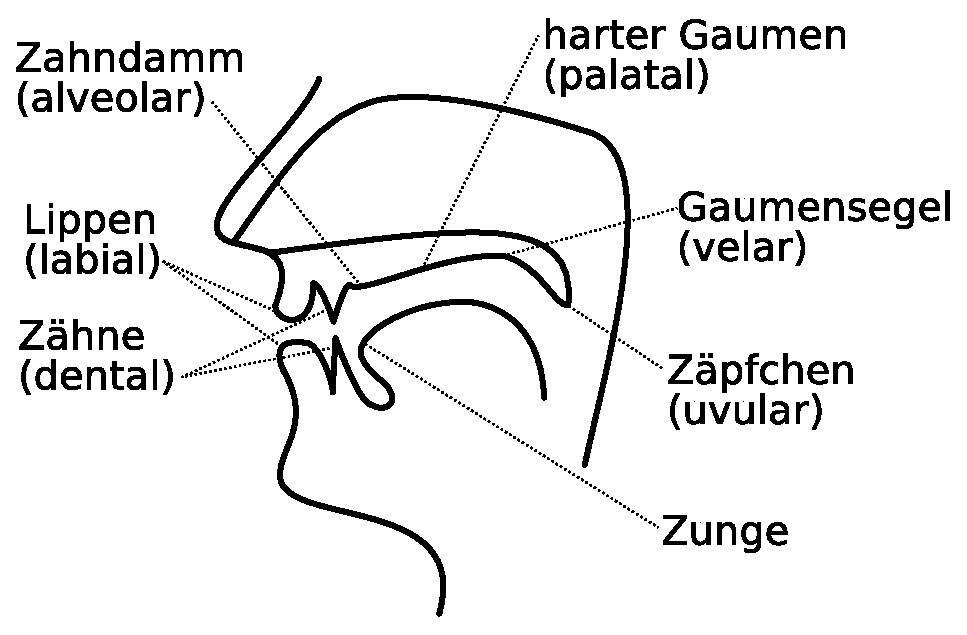
\includegraphics[width=0.5\textwidth]{figures/mundraum}
  \caption[Obere Sprechorgane und Artikulationsorte]{Obere Sprechorgane und Artikulationsorte}
  \label{fig:oberesprechorgane}
\end{figure}

Der Mundraum muss differenziert betrachtet werden, weil ein Großteil der Artikulation von Sprachlauten im Mundraum abläuft.
Einen schematischen Überblick zu den folgenden Betrachtungen gibt Abbildung~\ref{fig:oberesprechorgane}.
Eine wichtige Begrenzung des Mundraums nach unten ist die Zunge.
\TuBegin~Von Ihrer Zunge sehen Sie, wenn Sie sich vor den Spiegel stellen, nur den kleinsten Teil, nämlich den beweglichen Rücken und die bewegliche Spitze.
Der größte Teil der Zunge füllt den gesamten Bereich des Unterkiefers.
Auch hier gibt es die Möglichkeit, sich einen Eindruck davon zu verschaffen:
Fassen sie sich unter das Kinn (in den Bogen des Unterkiefers) und bewegen Sie die Zunge nach links und rechts.
Sie sollten spüren, wie sich größere muskuläre Strukturen bewegen.

Der bewegliche Teil der Zunge ist essentiell für die Bildung vieler Segmente.
Wenn wir den eigentlichen Mundraum von hinten nach vorne durchgehen, finden wir zunächst seine Begrenzung nach hinten: das \textit{Zäpfchen} (die \textit{Uvula}).
Am Zäpfchen werden tatsächlich Segmente des Deutschen gebildet, und zwar durch Anhebung des Zungenrückens.

Das \textit{Gaumensegel} (der \textit{weiche Gaumen}, das \textit{Velum}) ist ein weicher, mit Muskeln versorgter Abschnitt zwischen dem harten Gaumen und dem Zäpfchen.
Man kann das Gaumensegel ertasten, indem man mit der Zunge oder einem Finger vorsichtig im Gaumen nach hinten fährt.
Während der vordere Gaumen hart ist, folgt weiter hinten eine weiche Stelle direkt vor dem Zäpfchen.

Alle diese Teile der Mundhöhle spielen eine Rolle bei der Produktion standarddeutscher Segmente.
Eher eine indirekte Rolle bei der Sprachproduktion spielt die \textit{Nasenhöhle}.
\TuBegin~Halten Sie sich die Nase zu und sprechen Sie zunächst langanhaltend \textit{f} und \textit{s}, dann \textit{m} und \textit{n}.
Mit zugehaltener Nase sollte es nicht möglich sein, die \textit{m}- und \textit{n}-Segmente kontinuierlich auszusprechen.
Das liegt daran, dass bei diesen die Luft durch die Nasenhöhle statt durch die Mundhöhle abfließt.
Insofern ist die Nasenhöhle indirekt an der Produktion dieser Segmente beteiligt.

Zur weiteren Differenzierung des Gaumenbereichs spricht man bei der Stufe direkt hinter den Schneidezähnen vom \textit{Zahndamm} (die \textit{Alveolen}).
Den Zahndamm ertastet man auch sehr gut mit der Zungenspitze oder den Fingern.
Es handelt sich um die Stufe zwischen Zähnen und Gaumen.
Außerdem sind \textit{Zähne} und \textit{Lippen} an der Sprachproduktion beteiligt, wobei hier davon ausgegangen wird, dass der Ort und die sonstige Funktion dieser Körperteile hinlänglich bekannt ist.

\section{Artikulationsart}

\label{sec:artikulationsart}

\subsection{Passiver und aktiver Artikulator}

\label{sec:passiveraktiverartikulator}

Nachdem jetzt die an der Produktion deutscher Sprachlaute beteiligten Organe beschrieben wurden, müssen wir überlegen, wie diese Produktion genau abläuft.
Die Produktion des pulmonalen Luftstroms und des Stimmtons wurde schon beschrieben.
Im Grunde sind die einzigen Prinzipien der Produktion von Sprachlauten

\begin{enumerate}\Lf
  \item die \textit{Behinderung} (\textit{Obstruktion}) des Luftstroms, wodurch Geräusche (Zischen, Reiben, Knacken bzw.\ Knallen) entstehen, und
  \item die \textit{Veränderung von Resonanzen} der Mundhöhle durch Veränderung ihrer Form, was den Klang des Stimmtons verändert.
\end{enumerate}

Die Behinderung des Luftstroms findet an verschiedenen Stellen statt, und in diesem Zusammenhang sind zunächst die Begriffe \textit{aktiver und passiver Artikulator} zu erklären.
\TuBegin~Sprechen Sie langsam und sorgfältig das Wort \textit{Tante} und achten Sie darauf, wo sich die beweglichen Teile Ihres Mundraums jeweils befinden.
Sowohl die beiden \textit{t}-Segmente als das \textit{n}-Segment sind durch eine Berührung der Zunge an einer bestimmten Stelle innerhalb des Mundraums charakterisiert.
Versuchen Sie, die Stelle zu finden und anhand der Informationen aus Abschnitt~\ref{sec:anatomischegrundlagen} zu benennen, bevor Sie weiterlesen.

Beim \textit{t} und beim \textit{n} legt sich die vordere Zungenspitze gegen den Zahndamm.
Die Zunge ist dabei beweglich, der Zahndamm hingegen unbeweglich.
Dass sich zwei Körperteile auf diese Weise berühren bzw.\ annähern, ist charakteristisch für viele Artikulationen, und man nennt sie daher die \textit{Artikulatoren}.

\Definition{Artikulator}{
\label{def:artikulator}
Ein Artikulator ist ein Körperteil, der an einer Artikulation beteiligt ist.
Ein aktiver Artikulator führt dabei eine Bewegung zu einem sich nicht bewegenden passiven Artikulator aus.
\index{Artikulator}
}

Was die Artikulatoren bei welchen Segmenten genau machen, wird \textit{Artiulationsart} genannt und in den folgenden Abschnitten klassifiziert und illustriert.

\Definition{Artikulationsart}{\label{def:artart} Die Artikulationsart eines Segmentes ist die Art und Weise, in der der Luftstrom aus der Lunge durch die Artikulatoren behindert wird.}

\subsection{Stimmhaftigkeit}

\label{sec:stimmhaftigkeit}

Zunächst können wir eine grundlegende Unterscheidung in der Artikulationsart vornehmen.
In \ref{sec:kehlkopfrachen} wurde bereits beschrieben, dass manche Segmente mit Stimmton produziert werden, aber andere nicht.
Man kann also Segmente nach ihrer \textit{Stimmhaftigkeit} unterscheiden.

\Definition{Stimmhaftigkeit}{
Ein Segment ist stimmhaft, wenn zeitgleich zu seiner primären Artikulation ein Stimmton produziert wird.
\index{Stimmhaftigkeit}
}

\subsection{Obstruenten}

\label{sec:obstruenten}

Bei der zuerst zu besprechenden Gruppe von Segmenten handelt es sich um die sogenannten \textit{Obstruenten} (\textit{Geräuschlaute}, wörtlich im Latein eigentlich \textit{Hindernislaute}).
Nach der Definition folgen Abschnitte über die Unterarten von Obstruenten.

\Definition{Obstruent}{
Ein Obstruent ist ein Segment, bei dem der pulmonale Luftstrom durch eine Verengung, die die Artikulatoren herstellen, am freien Abfließen gehindert wird.
Es entstehen Geräuschlaute:
Entweder Knall- bzw.\ Knack-Laute oder Reibegeräusche durch Turbulenzen im Luftstrom.
\index{Obstruent}
}

Bei \textit{k}-, \textit{t}- und \textit{p}-Segmenten (ähnlich \textit{g}, \textit{d}, \textit{b}) wird der Luftstrom jeweils kurz unterbrochen, und nach der Unterbrechung folgt ein deutlicher Schwall von Luft, der dann wieder abebbt.
Das liegt daran, dass die Artikulatoren einen vollständigen Verschluss des Mundraumes herstellen, der dann spontan gelöst wird.
Das entstehende Geräusch ähnelt einem Knall, und die betreffenden Segmente heißen \textit{Plosive}.
\TuBegin~Halten Sie sich eine Handfläche dicht vor den Mund und sprechen Sie folgende Wörter sorgfältig aus: \textit{Kuckuck}, \textit{Torte}, \textit{Pappe}.
Es fällt sofort auf, dass der Luftstrom nicht gleichmäßig (wie beim einfachen Atmen) aus dem Mund entweicht.

\Definition{Plosiv}{
Ein Plosiv ist ein Obstruent, bei dem einer totalen Verschlussphase eine Lösung des Verschlusses folgt und ein Knall- oder Knackgeräusch entsteht.
\index{Plosiv}
}

Plosive können -- wie bereits erwähnt -- nach Stimmhaftigkeit unterschieden werden, wie an den Wörtern \textit{danke}/\textit{tanke}, \textit{banne}/\textit{Panne}, \textit{Gabel}/\textit{Kabel} demonstriert werden kann.
Hier entsprechen jeweils \textit{d} und \textit{t}, \textit{b} und \textit{p} sowie \textit{g} und \textit{k} einem stimmhaften und einem stimmlosen Segment.

Das Geräusch, das bei \textit{Frikativen} entsteht, kann als Rauschen (oder Reibegeräusch) beschrieben werden.
Daher kommt auch der Name, der mit \textit{Reibelaute} eingedeutscht werden kann.
\TuBegin~Sprechen und fühlen Sie folgende Wörter: \textit{Skischuhe}, \textit{Fach}, \textit{Wicht}.
Bei den Segmenten, die durch \textit{sch} (und in \textit{Ski} ausnahmsweise \textit{sk}), \textit{f}, \textit{ch} und \textit{w} wiedergegeben werden, spüren Sie ein konstantes, mehr oder weniger scharfes Entweichen von Luft.

\Definition{Frikativ}{
Ein Frikativ ist ein Obstruent, bei dem durch die Artikulatoren eine vergleichsweise enge aber nicht vollständige Verengung im Weg des pulmonalen Luftstroms hergestellt wird, wodurch dieser stark verwirbelt wird (Turbulenzen) und ein rauschendes Geräusch erzeugt wird.
\index{Frikativ}
}

Bemerkenswert ist außerdem, dass die Frikative (im Gegensatz zu den Plosiven) so lange artikuliert werden können, wie der Luftstrom aufrecht erhalten werden kann.
Die Segmente sind also \textit{kontinuierlicher} als Plosive.
Auch unter den Frikativen gibt es stimmlose und stimmhafte: \textit{sch}, \textit{ch} und \textit{f} sind stimmlos, \textit{w}-Laute aber \zB stimmhaft.
Auch das \textit{j}-Segment (\textit{Jahr}) wird im Normalfall als Frikativ artikuliert, alternativ als \textit{Approximant} (s.\ Abschnitt~\ref{sec:lateraleapproximanten}).

\textit{Affrikaten} sind komplexe Segmente, nämlich eine direkte Abfolge von einem Plosiv und einem Frikativ.
Beispiele sind das \textit{ts}-Segment (orthographisch \textit{z}) in Wörtern wie \textit{Zuschauer} oder das \textit{pf}-Segment wie in \textit{Pfund}.

\Definition{Affrikate}{
\label{def:affrikate}
Eine Affrikate ist ein komplexer Obstruent aus einem Plosiv und einem folgenden Frikativ.
Der beteiligte Plosiv und der beteiligte Frikativ sind dabei \textit{homorgan} (an derselben Stelle gebildet).
\index{Affrikate}
}

Die deutschen \textit{pf}-Segmente sind \zB streng genommen nicht homorgan, wie in Abschnitt~\ref{sec:affrikatenartikulationsorte} erläutert wird.
Die Frage, ob wirklich eine Affrikate oder doch zwei Segmente vorliegen, ist oft nur schwer zu entscheiden und manchmal eher eine Frage der Phonologie als der Phonetik.

\subsection{Approximanten}

\label{sec:lateraleapproximanten}

Im Deutschen ist das \textit{l}-Segment das einzige, dass zuverlässig als \textit{Approximant} artikuliert wird.
Bei einem Approximanten werden die Artikulatoren ähnlich wie beim Frikativ angenähert, aber es entstehen keine Turbulenzen
\TuBegin~Beobachten Sie (möglichst vor dem Spiegel), wie im Wort \textit{Ball} das letzte Segment gebildet wird.

Beim \textit{l}-Segment wird die Zungenspitze mittig an den Zahndamm gelegt, seitlich der Zunge fließt der Luftstrom aber ungehindert ab.
Die seitliche Öffnung ist charakteristisch für den \textit{lateralen Approximanten}.
Wenn das \textit{j}-Segment nicht als stimmhafter Frikativ, sondern als Approximant artikuliert wird, nähert sich der Zungenrücken dem harten Gaumen.
Dabei fließt der Luftstrom durch die Mitte des Mundraums ab, und man spricht von einem \textit{zentralen Approximanten}.

\Definition{Approximant}{
Ein Approximant ist ein Segment, bei dem sich die Artikulatoren stark annähern und der Luftstrom kontinuierlich durch die Verengung abfließt.
Anders als beim Frikativ ist die Annäherung aber nicht so stark, dass Turbulenzen und damit ein Reibegeräusch entstehen.
Beim \textit{zentralen} Approximanten fließt das Luftvolumen hauptsächlich durch die Mitte des Mundraums ab.
Beim \textit{lateralen} Approximanten wird im Mundraum durch die Zunge als aktiver Artikulator ein Verschluss hergestellt, und die eigentliche Verengung, durch die die Luft abfließt, befindet sich seitlich dieses Verschlusses.
\index{Approximant}
}

\subsection{Nasale}

\label{sec:nasale}

Wir haben bereits den Test gemacht, Wörter mit \textit{n} und \textit{m} mit zugehaltener Nase auszusprechen, und dabei festgestellt, dass dies unmöglich ist.
Bei diesen beiden Segmenten handelt es sich um \textit{Nasale}.
Bei Nasalen wird der Mundraum vollständig verschlossen, die Luft kann nirgendwohin entweichen, und die Artikulation wird unmöglich.
Dass wir verschiedene nasale Obstruenten akustisch voneinander unterscheiden können, liegt wieder an unterschiedlichen Resonanzen, genauso wie bei den Approximanten und den Vokalen (s.\ Abschnitt~\ref{sec:vokale}).

\Definition{Nasal}{
Ein Nasal ist ein Segment, bei dem durch einen vollständigen Verschluss im Mundraum (und eine Absenkung des Velums) die Luft zum Entweichen durch die Nasenhöhle gezwungen wird.
Es entstehen keine Turbulenzen.
\index{Nasal}
}

\subsection{Vokale}

\label{sec:vokale}

\textit{Vokale} werden in der Schulgrammatik gerne als \textit{Selbstlaute} bezeichnet und damit den Konsonanten als \textit{Mitlauten} gegenübergestellt.
Die Idee hinter dieser Bezeichnung ist, dass die Vokale selbständig (also für sich allein) ausgesprochen werden können, wohingegen die Konsonanten nur mit einem anderen Segment (einem Vokal) zusammen ausgesprochen werden können.
Diese Einordnung ist grundlegend falsch, da alle Konsonanten (ggf.\ nach entsprechendem phonetischen Training) selbständig realisiert werden können.
Bei Frikativen und Nasalen ist sogar die kontinuierliche Artikulation möglich.
Da wir einen intuitiven Begriff von Vokalen haben und die orthographisch als \textit{a}, \textit{e}, \textit{i}, \textit{o}, \textit{u} sowie \textit{ä}, \textit{ö}, \textit{ü} wiedergegebenen Segmente als Vokale bereits kennen, können wir überlegen, was das Besondere an ihnen ist.
\TuBegin~Sprechen Sie sich die Vokalsegmente vor und beobachten Sie dabei (einschließlich Beobachtung im Spiegel), wie sich die Zunge, die Lippen und die sonstigen Organe im Mundraum dabei verhalten. Wenn Sie bei der Produktion von Vokalen wieder Ihren Kehlkopf ertasten, werden Sie außerdem feststellen, dass alle stimmhaft sind.

Die Zunge bewegt sich bei der Artikulation verschiedener Vokale im Mund\-raum zu verschiedenen Positionen, aber es findet bei keinem der Segmente eine deutliche Verengung an irgendeinem Artikulator statt.
Der Luftstrom kann daher weitgehend ungehindert abfließen.
Außerdem verändert sich die Formung der Lippen von rund (\zB bei \textit{u}) zu eher breit (\zB bei \textit{e}).

\Definition{Vokal}{
\label{def:vokal}
Ein Vokal ist ein Segment, bei dem der pulmonale Luftstrom weitgehend ungehindert abfließen kann, und bei dem keine geräuschhaften Anteile entstehen.
Der Klang eines Vokals wird durch eine spezifische Formung des Resonanzraumes erzeugt.
\index{Vokal}
}

Man muss an dieser Stelle wenigstens intuitiv definieren, was Resonanzen sind.
Das Phänomen, dass physikalische Körper abhängig von ihrer Form und ihrem Material einen Klang verändern, der in ihnen produziert wird, lässt sich leicht nachvollziehen.
Wenn man in ein Rohr aus Holz, in ein Metallrohr, in die hohle Hand oder in einen hohlen Betonklotz einen Ton singt, klingt dieser jeweils unterschiedlich.
Das liegt daran, dass ein Körper abhängig von seinem Material, seiner Form und Größe bestimmte Frequenzen eines Klangs verstärkt und abschwächt.
Körper haben also ein charakteristisches \textit{Resonanzverhalten} abhängig von Form und Material.
Das Resonanzverhalten des Mundraums wird nun bei Vokalen gezielt durch die Positionierung der Zunge und der Lippen verändert, denn durch die Positionierung dieser Artikulatoren ändert sich die Form des Mundraums.
Wir können also \textit{a} und \textit{i} voneinander unterscheiden, weil das Ausgangssignal des Stimmtons bei diesen Segmenten jeweils mit einem unterschiedlich geformten Mundraum zu einem anderen Klang geformt wird.

\subsection{Oberklassen für Artikulationsarten}

\label{sec:oberklassenfuerartikulationsarten}

Bei den Vokalen, Approximanten und Nasalen enthielten die Definitionen jeweils das Kriterium, dass keine Turbulenzen entstehen, während der Luftstrom abfließt.
Außerdem gibt es natürlich bei diesen Segmenten keine spontane Verschlusslösung mit Knallgeräusch wie bei den Plosiven.
Daher gibt es hier den Oberbegriff des \textit{Sonoranten}, der diese Segmente zusammenfasst und den Obstruenten gegenüberstellt.
Typisch, aber nicht notwendig für die Sonoranten ist die Stimmhaftigkeit.

\Definition{Sonoranten und Obstruenten}{
Sonoranten (Klanglaute) sind nicht-geräuschhafte Segmente, bei denen der pulmonale Luftstrom ohne Bildung von Turbulenzen durch den Mund oder die Nase abfließen kann.
Alle anderen Segmente gelten als geräuschhaft und werden Obstruenten (Geräuschlaute) genannt.
\index{Sonorant}
\index{Obstruent}
}

\Satz{Sonoranten und Stimmton}{
Sonoranten sind prototypisch stimmhaft.
}

Die Unterscheidung von Vokalen und Konsonanten hat nichts mit der Unterscheidung von Sonoranten und Obstruenten zu tun.
Die Konsonanten sind eine Sammelklasse für alle Sonoranten und Obstruenten, die keine Vokale sind.

\Definition{Konsonanten}{
Konsonanten sind alle Obstruenten, Approximanten und Nasale.
Es sind die Segmente, die typischerweise (aber nicht notwendigerweise) nicht silbisch sind, also prototypischerweise alleine keine Silbe bilden können.
\index{Konsonant}
}

Damit ergibt sich das Diagramm in \ref{fig:lautklassen} für die Klassifizierung der Segmente in der Phonetik.
In Abschnitt~\ref{sec:phonetischemerkmale} wird gezeigt, dass diese Klassifizierung einen echten Erklärungsvorteil mit sich bringt.

\begin{figure}
  \centering
  \Treek[2.5]{4}{
    & \K{\textbf{Sonoranten}}\Below{(Klanglaute)}\BBel{dl}\BBel{d}\BBel{dr} &&& \K{\textbf{Obstruenten}}\Below{(Geräuschlaute)}\BBel{dl}\BBel{d}\BBel{dr} \\
    \K{\textbf{Vokale}}\Below{(silbisch)} & \K{Approximanten}\B{drr} & \K{Nasale}\B{dr} & \K{Plosive}\B{d} & \K{Frikative}\B{dl} & \K{Affrikaten}\B{dll} \\
    &&& \K{\textbf{Konsonanten}}\Below{(nicht silbisch)} \\
  }
  \caption{Grobe Klassifikation der Segmente in der Phonetik}
  \label{fig:lautklassen}
\end{figure}

\section{Artikulationsort}

\label{sec:artikulationsort}

Bisher haben wir uns darauf beschränkt, festzustellen, auf welche Art bestimmte Segmente gebildet werden.
In einigen Fällen (\zB beim \textit{l}-Segment) haben wir auch schon festgestellt, wo die Artikulatoren ggf.\ einen Verschluss oder eine Annäherung herstellen, aber das muss noch systematisch geschehen.
Dabei leitet uns Definition~\ref{def:artort}.
Gleichzeitig werden die für die Transkription des Deutschen benötigten Zeichen des weitest verbreiteten phonetischen Alphabets vorgestellt.

\Definition{Artikulationsort}{\label{def:artort} Der Artikulationsort eines Segments ist der Punkt der größten Annäherung zwischen den Artikulatoren.}

\subsection{Das IPA-Alphabet}

\label{sec:ipaalphabet}

\index{IPA}

Das übliche phonetische Alphabet ist das der \textit{International Phonetic Association} (IPA).%
\footnote{\url{https://www.internationalphoneticassociation.org/}}	
Es basiert auf der Lateinschrift und stellt für alle in menschlichen Sprachen vorkommenden Segmente eine mögliche Schreibung zur Verfügung.
Dabei werden primäre Artikulationen in der Regel durch ein Buchstabensymbol dargestellt.
Hinzu kommen sog.\ Diakritika (Zusatzzeichen), die vor, über, unter oder neben dem Hauptzeichen geschrieben werden und genauere Informationen zur primären Artikulation kodieren.
Hier besteht also tatsächlich der Anspruch, ein System vorzulegen, in dem man so schreibt, wie man spricht (vgl.\ Abschnitt~\ref{sec:orthographiegraphematik}).

Es ist üblich, phonetische Transkriptionen in [~] zu schreiben, und wir übernehmen hier diese Konvention.
Man unterscheidet gemeinhin eine enge Transkription von einer weiten oder lockeren Transkription.
Bei einer engen Transkription versucht man, jedes artikulatorische Detail, das man hört, genau festzuhalten, auch die linguistisch vielleicht irrelevanten.
Bei der lockeren Transkription geht es nur darum, die wichtigen Merkmale der gehörten Segmente aufzuschreiben.
Die lockere Transkription ist prinzipiell problematisch, weil sie dazu tendiert, zu viel phonologisches Wissen in die Transkription einzubeziehen.
Eine phonetische Transkription sollte im Normalfall so beschaffen sein, dass sie genau wiedergibt, was man tatsächlich gehört hat.
Da es hier aber nur um einen ersten Einblick geht, ist unsere Transkription nicht übermäßig genau, möglichst ohne dass sich dabei verfälschende Vereinfachungen einschleichen.

\subsection{Laryngale}

\label{sec:laryngale}

\index{Laryngal}

Im Bereich des Kehlkopfs (Larynx) bzw.\ des Stimmlippensystems (Glottis) bilden Sprecher des Standarddeutschen nur zwei Segmente.%
\footnote{Für normale phonetische Belange ist die Unterscheidung von Glottis und Larynx nicht relevant, und man findet sowohl die Bezeichnung \textit{glottal} als auch \textit{laryngal}.}
Der eine ist der stimmlose laryngale Frikativ \textipa{[h]}.
In Wörtern wie \textit{Hupe}, \textit{Handspiel} usw.\ kommt dieses Segment am Anfang vor.
Weiterhin ist der stimmlose laryngale Plosiv \textipa{[P]} sehr charakteristisch für das Deutsche.
\TuBegin~Wenn Sie Wörter wie \textit{Anpfiff} oder \textit{energisch} sehr deutlich und energisch aussprechen, hören Sie am Anfang des Wortes einen Plosiv, einen Knacklaut im Kehlkopf.
Er tritt auch vor dem \textit{o} in \textit{Chaot} (nicht aber in \textit{Chaos}), vor dem \textit{ei} in \textit{Verein} oder vor dem \textit{äu} in \textit{beäugen} auf.

Bei diesem bilden die Stimmlippen als aktive Artikulatoren einen Verschluss, der spontan gelöst wird.
Wenn wir das IPA-Zeichen \textipa{P} vorläufig in die normale Orthographie einfügen, ergibt sich für die obigen Wörter (\ref{ex:phot2529}).

\begin{exe}
  \ex\label{ex:phot2529}
  \begin{xlist}
    \ex{\textipa{P}Anpfiff}
    \ex{\textipa{P}energisch}
    \ex{Cha\textipa{P}ot}
    \ex{Chaos, \Ast Cha\textipa{P}os}
    \ex{Ver\textipa{P}ein}
    \ex{be\textipa{P}äugen}
  \end{xlist}
\end{exe}

\index{Glottalverschluss}
Dieser laryngale Plosiv (auch \textit{Glottalverschluss}, \textit{Glottisverschluss} oder englisch \textit{glottal stop}) tritt regelhaft vor jedem vokalisch anlautenden Wort und auch vor jeder vokalisch anlautenden betonten Silbe innerhalb eines Wortes auf.
Zur Wortbetonung (dem \textit{Akzent}) wird in Abschnitt~\ref{sec:wortakzent} mehr Substantielles gesagt.
Dort wird die Regel für die \textipa{[P]}-Einfügung weiter motiviert und illustriert.
Viele Sprachen haben einen vokalischen Anlaut ohne diesen Plosiv.
Er ist daher typisch für einen deutschen Akzent in vielen Fremdsprachen, der oft als abgehackt wahrgenommen wird.
Umgekehrt ist sein Fehlen verantwortlich dafür, dass fremdsprachliche Akzente im Deutschen von Erstsprechern des Deutschen oft als konturlos o.\,ä.\ wahrgenommen werden.

\subsection{Uvulare}

\label{sec:uvulare}

\index{Uvular}

Am Zäpfchen werden der stimmlose und der stimmhafte uvulare Frikativ gebildet: \textipa{[X]} und \textipa{[K]}.
Der stimmlose wird \textit{ch} geschrieben und tritt nur nach bestimmten Vokalen auf, also in Wörtern wie \textit{ach}, \textit{Bach}, \textit{Tuch}.%
\footnote{Die oft zu findende Behauptung, in Wörtern wie \textit{Buch} handele es sich im deutschen Standard um einen am weichen Gaumen artikulierten Velar \textipa{[x]} (s.\ Abschnitt~\ref{sec:velare}) kann ich nicht nachvollziehen.
Außer evtl.\ in Dialekten wie dem Sauerländischen findet die Artikulation gut hörbar weiter hinten im Mundraum statt, also am Zäpfchen.
}
Der stimmhafte kommt nicht bei allen Sprechern des Deutschen vor, ist aber die häufigste phonetische Realisierung von \textit{r} im Silbenanlaut, also in \textit{rot}, \textit{berauschen} usw.
\TuBegin~Zur bewussten Lokalisierung von \textipa{[X]} und \textipa{[K]}, die im hinteren Bereich der Mundhöhle gebildet werden, hilft es, die vordere Zunge mit einem geeigneten Gegenstand herunterzudrücken und dann \zB \textit{Rache} zu sagen (mit \textipa{[K]} und \textipa{[X]}).
Das klingt zwar wegen der eingeschränkten Artikulation der Vokale etwas ungewöhnlich, die Konsonanten können aber einwandfrei realisiert werden.
Hier ist zwar die Zunge der aktive Artikulator, aber nur mit dem hinteren Teil, dem Zungenrücken.

\subsection{Velare}

\label{sec:velare}

\index{Velar}

Das Velum oder Gaumensegel ist einer von mehreren Artikulationsorten, an denen im Deutschen ein stimmloser und ein stimmhafter Plosiv sowie ein Nasal artikuliert werden.
\TuBegin~Halten Sie wieder die Zungenspitze fest und artikulieren Sie \textit{King Kong} und \textit{Gang}.
Die Artikulation sollte ähnlich gut gelingen wie bei \textit{Rache}, weil auch hier die Zungenspitze nicht beteiligt ist.
Mit ein bisschen Mühe ist es möglich, den Ort und die Art der Artikulation dieser Segmente im Selbstversuch auch visuell zu beobachten.
Dazu stellt man sich vor einen Spiegel und lässt den Mund so weit wie möglich geöffnet bei der Artikulation der Beispielwörter.
Man kann dann sehen, wie sich der Zungenrücken an das Gaumensegel hebt, und wie ggf.\ der Verschluss gelöst wird.

Die \textit{k}-, \textit{g}- und \textit{ng}-Segmente werden also alle im hinteren Mundraum artikuliert, und zwar am Velum.
Der Zungenrücken ist dabei der aktive Artikulator.
Die IPA-Schreibungen sind sehr transparent: \textipa{[k]}, \textipa{[g]} und \textipa{[N]}.
Zu beachten ist, dass orthographisches \textit{ng} zumindest in der Phonetik einem Laut und nicht etwa zwei Lauten entspricht.

\subsection{Palatale}

\index{Palatal}

Am harten Gaumen finden wir im Deutschen nur das \textit{j}-Segment wie in \textit{Jahr}, \textit{Jugend} usw. und den so genannten \textit{ich}-Laut.
Das \textit{j}-Segment wird meist als palataler stimmhafter Frikativ \textipa{[J]} realisiert.
Der \textit{ich}-Laut hingegen ist immer ein palataler stimmloser Frikativ \textipa{[\c{c}]}.

\subsection{Palatoalveolare und Alveolare}

\label{sec:palatoalveolarealveolare}

\index{Alveolar}
\index{Palatoalveolar}

Am Übergang vom harten Gaumen zum Zahndamm und am Zahndamm finden sich eine ganze Reihe von Segmenten in verschiedenen Artikulationsarten, sowohl stimmlos als auch stimmhaft.
\TuBegin~Sprechen Sie die folgenden Wörter und achten Sie auf die Anlaute: \textit{lang}, \textit{schön}, \textit{Tor}, \textit{Didi}.
Diese Segmente werden am unteren Teil des Zahndamms gebildet.
Wenn Sie in diesem Fall die Zungenspitze festhalten, können Sie diese Wörter nicht auf verständliche Weise aussprechen.

Die hier besprochenen Segmente werden im Gegensatz zu den Uvularen und Velaren mit der Zungenspitze als aktivem Artikulator gebildet.
Das \textit{l}-Segment ist der palatoalveolare laterale Approximant und wird \textipa{[l]} transkribiert.
Das \textit{sch}-Segment, bei dem meistens zusätzlich die Lippen rund geformt werden, wird \textipa{[S]} transkribiert.
Zusätzlich gibt es noch den stimmhaften palatoalveolaren Frikativ \textipa{[Z]} wie in \textit{Garage}, \textit{Marge} oder anderen, meist französischen Lehnwörtern.
Weil diese Wörter nicht zum Kernwortschatz gehören (s.\ Abschnitt~\ref{sec:kernundperipherie}), lassen wir \textipa{[Z]} im weiteren Verlauf aus Übersichtstabellen usw.\ heraus.
Etwas weiter vorne werden die Anlaute folgender Wörter gesprochen, ebenfalls mit der Zungenspitze als aktivem Artikulator: \textit{Tor}, \textit{dort}, \textit{neu}, \textit{Sahne}.
Gleiches gilt für das letzte Segment in folgendem Wort: \textit{Schluss}.
Wir haben hier eine komplette Reihe von alveolarem stimmlosen Plosiv \textipa{[t]}, alveolarem stimmhaften Plosiv \textipa{[d]}, alveolarem Nasal \textipa{[n]}, alveolarem stimmhaften Frikativ \textipa{[z]} (wie in \textit{Sahne}) und alveolarem stimmlosen Frikativ \textipa{[s]} wie in \textit{Schluss}.%
\footnote{Die Segmente \textipa{[s]} und \textipa{[z]} werden dabei eigentlich etwas weiter vorne in Richtung der Zähne artikuliert.}

\subsection{Labiodentale und Bilabiale}

\index{Labial}

Im Bereich der Konsonanten sind wir von unten nach oben und hinten nach vorne durch den Vokaltrakt vorgegangen und erreichen jetzt den Bereich der Lippen.
\TuBegin~Vor dem Spiegel sieht man gleich, dass Wörter wie \textit{Pass} oder \textit{Ball} mit einem an der gleichen Stelle artikulierten Segment beginnen.
Beide Lippen (als aktive Artikulatoren) schließen sich und lösen daraufhin den Verschluss.
Es handelt sich um den stimmlosen bilabialen Plosiv \textipa{[p]} und den stimmhaften bilabialen Plosiv \textipa{[b]}.

Während bei den zuletzt genannten Segmenten beide Lippen beteiligt sind (daher der Terminus \textit{bilabial}), erkennt man bei den Anlauten von \textit{Fuß} und \textit{Wade}, dass die Zähne des Oberkiefers beteiligt sind, die sich an die Unterlippe legen.
Dort erzeugen sie keinen Verschluss, sondern eine Verengung mit Reibegeräusch.
Es handelt sich daher um den stimmlosen und den stimmhaften \textit{labio-dentalen} Frikativ (\textipa{[f]} und \textipa{[v]}).

\subsection{Affrikaten und Artikulationsorte}

\label{sec:affrikatenartikulationsorte}

\index{Affrikate!Homorganität}

In den Wörtern \textit{Dschungel}, \textit{Chips}, \textit{Zange}, \textit{Pfanne} finden wir anlautend das gesamte Inventar der phonetischen Affrikaten im Deutschen.
Diese bestehen aus zwei aufeinanderfolgenden Phasen: einer plosiven Phase und einer frikativen Phase.
Man schreibt im IPA-Alphabet daher diese Segmente mit den Grundzeichen für den Plosiv und den Frikativ mit einem verbindenden Bogen (der \textit{Ligatur}) darüber.
Für die stimmlose palatoalveolare Affrikate wie in \textit{Matsch} ergibt sich also \textipa{[\t{tS}]}, für die stimmlose alveolare Affrikate wie in \textit{Zange} \textipa{[\t{ts}]} und für die stimmlose labiale Affrikate wie in \textit{Pfanne} \textipa{[\t{pf}]}.
Nur in Lehnwörtertn findet man die stimmhafte palatoalveolare Affrikate wie in \textit{Dschungel}, transkribiert \textipa{[\t{dZ}]}.

Wenn wir uns \textipa{[\t{pf}]} ansehen, stellen wir fest, dass die Bedingung der Homorganität aus Definition~\ref{def:affrikate} (S.~\pageref{def:affrikate}) strenggenommen nicht erfüllt wird, denn \textipa{[p]} ist bilabial und \textipa{[f]} labio-dental.
Insofern werden die beiden Teile der Affrikate zwar ziemlich nah beieinander gebildet, aber nicht wirklich am selben Ort.
Ohne uns in die Details dieses Problems zu vertiefen, stellen wir dies hier fest, behandeln \textipa{[\t{pf}]} aber im weiteren Verlauf als Affrikate.

\begin{table}
  \centering
  \begin{tabular}{rccccccccc}
    \lsptoprule
    \multicolumn{1}{c}{} & \Sw{\textbf{bilabial}} & \Sw{\textbf{labio-dental}} & \Sw{\textbf{alveolar}} & \Sw{\textbf{palatoalveolar}} & \Sw{\textbf{palatal}} & \Sw{\textbf{velar}} & \Sw{\textbf{uvular}} & \Sw{\textbf{laryngal}} \\
    \midrule
    \textbf{stl.\ Plosiv} & \textipa{p} & \textipa{} & \textipa{t} & \textipa{} & \textipa{} & \textipa{k} & \textipa{} & \textipa{P} \\
    \textbf{sth.\ Plosiv} & \textipa{b} & \textipa{} & \textipa{d} & \textipa{} & \textipa{} & \textipa{g} & \textipa{} & \textipa{} \\
    \textbf{stl.\ Frikativ} & \textipa{} & \textipa{f} & \textipa{s} & \textipa{S} & \textipa{\c{c}} & \textipa{} & \textipa{X} & \textipa{h} \\
    \textbf{sth.\ Frikativ} & \textipa{} & \textipa{v} & \textipa{z} & \textipa{} & \textipa{J} & \textipa{} & \textipa{K} & \textipa{} \\
    \textbf{stl.\ Affrikate} & \textipa{} & \textipa{\t{pf}} & \textipa{\t{ts}} & \textipa{\t{tS}} & \textipa{} & \textipa{} & \textipa{} & \textipa{} \\
    \textbf{sth.\ Affrikate} & \textipa{} & \textipa{} & \textipa{} & \textipa{} & \textipa{} & \textipa{} & \textipa{} & \textipa{} \\
    \textbf{lateraler Approximant} & \textipa{} & \textipa{} & \textipa{} & \textipa{l} & \textipa{} & \textipa{} & \textipa{} & \textipa{} \\
    \textbf{Nasal} & \textipa{m} & \textipa{} & \textipa{n} & \textipa{} & \textipa{} & \textipa{N} & \textipa{} & \textipa{} \\
    \lspbottomrule
  \end{tabular}
  \caption{IPA:\ Konsonanten des Deutschen}
  \label{tab:photkons}
\end{table}

\subsection{Vokale und Diphthonge}

\label{sec:vokalediphthonge}

\index{Vokal}

Für die phonetische Klassifikation der Vokale werden in diesem Abschnitt \textit{Höhe} und \textit{Lage} als eine Art vokalischer Artikulationsort eingeführt.
Außerdem werden \textit{Rundung} und \textit{Länge} diskutiert, die strenggenommen nicht zum Artikulationsort gehören.%
\footnote{Die IPA-Symbole sind nun nahezu vollständig eingeführt und alle Beispielwörter werden ab jetzt vollständig transkribiert.}
Man fasst die Vokale normalerweise in einem sogenannten \textit{Vokalviereck} (manchmal auch \textit{Vokaltrapez} genannt) zusammen, s.\ Tabelle~\ref{tab:vokaltrap}.
Das Vokalviereck ist nichts anderes als eine Tabelle, in der die Spalten die Lage und die Zeilen die Höhe kodieren.
Wenn es eine ungerundete und eine gerundete Variante gibt, steht die gerundete stets an zweiter Stelle.
Länge wird hier nicht verzeichnet.
Der Rest dieses Abschnitts erläutert das Vokalviereck im Detail.

\index{Vokalviereck}

\begin{table}
  \centering
  \begin{tabular}{cccccc}
    \lsptoprule
    \multicolumn{1}{c}{} && \textbf{halb-} && \textbf{halb-} & \\
    \multicolumn{1}{c}{} & \textbf{vorne} & \textbf{vorne} & \textbf{zentral} & \textbf{hinten} & \textbf{hinten} \\
    \midrule
    \textbf{hoch/geschlossen} & \textipa{i y} &&&& \textipa{u} \\
    \multirow{2}{*}{\textbf{halbhoch}} && \textipa{I Y} && \textipa{U} & \\
    & \textipa{e} \textipa{\o} &&&& \textipa{o} \\
    \textbf{mittel} &&& \textipa{@} && \\
    \multirow{2}{*}{\textbf{halbtief}}& \textipa{E} \textipa{\oe} &&&& \textipa{O} \\
    &&& \textipa{5} && \\
    \textbf{tief/offen} &&& \textipa{a} && \\
    \lspbottomrule
  \end{tabular}
  \caption{IPA-Vokalviereck für das Deutsche}
  \label{tab:vokaltrap}
\end{table}

Vokale sind gewöhnlicherweise bezüglich ihres Artikulationsorts schwerer einzuordnen als Konsonanten.
Dies liegt daran, dass es für Vokale keinen gut lokalisierbaren punktuellen Artikulationsort gibt und die Orientierung im Mundraum dadurch erschwert wird.
Vielmehr wird die Zunge (sehr vereinfacht gesprochen) höher oder tiefer und weiter vorne oder weiter hinten im Mundraum lokalisiert.
Entsprechend unterscheidet man Vokale nach ihrer \textit{Lage} als \textit{vorne}, \textit{zentral} oder \textit{hinten} und ihrer \textit{Höhe} als \textit{hoch}, \textit{mittel} oder \textit{tief}.
Wenn Zwischenstufen benötigt werden, heißen diese \textit{halbvorne}, \textit{halbhinten} und \textit{halbhoch}, \textit{halbtief}.
Somit hat man auf beiden Achsen eine fünffache Unterscheidung, die insbesondere in der Phonologie ggf.\ durch elegantere Formulierungen reduziert werden kann.
Hohe Vokale kommen beispielsweise in \textit{lieb} \textipa{[li:p]}, \textit{lüg} \textipa{[ly:k]}, \textit{Trug} \textipa{[tKu:k]} vor, wobei \textipa{[i]} und \textipa{[y]} vorne liegen und \textipa{[u]} hinten.
Der tiefste Vokal ist \textipa{[a]} wie in \textit{Lab} \textipa{[la:p]}.

\index{Lippenrundung}
Weiterhin werden Vokale nach \textit{Lippenrundung} weiter unterschieden.
Der einzige Unterschied zwischen \textipa{[i]} in \textit{Liege} \textipa{[li:g@]} und \textipa{[y]} in \textit{Lüge} \textipa{[ly:g@]} oder \textipa{[e]} in \textit{Wege} \textipa{[ve:g@]} und \textipa{[\o]} in \textit{wöge} \textipa{[v\o:g@]} ist also der der Rundung.
\TuBegin~Wenn Sie wieder ein Spiegel-Experiment machen und zunächst \textit{u}, \textit{o}, \textit{ü} und \textit{ö} sprechen und dann \textit{a}, \textit{i}, \textit{e} und \textit{ä}, dann werden Sie beobachten, dass bei der Artikulation der ersten Gruppe die Lippen gerundet sind, bei der zweiten Gruppe aber nicht.

Die \textit{Länge} bezieht sich schließlich auf die Zeitdauer, für die ein Segment artikuliert wird.
Das ist nicht absolut zu verstehen, in dem Sinn, dass lange und kurze Vokal eine bestimmte Zeit von Millisekunden dauern, sondern relativ zueinander.
Es gibt von bestimmten Vokalen -- nämlich \textipa{[i]}, \textipa{[y]}, \textipa{[u]}, \textipa{[e]}, \textipa{[\o]}, \textipa{[o]} und \textipa{[a]} -- eine lange und eine kurze Variante.
Die lange Variante kommt in betonten Silben vor (\textipa{[i:]} in \textit{Liebe} \textipa{[li:b@]}, \textipa{[e:]} wie in \textit{Weg} \textipa{[ve:k]}), die kurze in unbetonten (\textipa{[i]} und \textipa{[o]} in \textit{Lithographie} \textipa{[litogKafi:]}, \textipa{[e]} wie in \textit{Methyl} \textipa{[mety:l]}).
Alle anderen Vokale sind immer kurz, auch wenn sie betont werden (\textipa{[I]} wie in \textit{Rinde} \textipa{[KInd@]}).
In Abschnitt~\ref{sec:gespanntheitbetonunglaenge} in der Phonologie wird eine Analyse der Längenverhältnisse vorgeschlagen.

\index{Schwa}
In der Tabelle findet sich schließlich noch ein besonderes Segment, nämlich das sogenannte \textit{Schwa} \textipa{[@]}.
Das Schwa ist ein \textit{Zentralvokal}, denn er steht in jeder Hinsicht in der Mitte der Vokalvierecks.
Besser ist evtl.\ die Bezeichnung \textit{Reduktionsvokal}, altertümlich hingegen \textit{Murmelvokal}.
Schwa kommt nur unbetont vor, \zB in der zweiten Silbe von Wörtern wie \textit{Tage} \textipa{[ta:g@]} oder \textit{geben} \textipa{[ge:b@n]}.
Außerdem wird (unbetontes) orthographisches \textit{-er} nach vorangehendem Konsonanten in der Liste immer als \textipa{[5]} (auch unglücklich als \textit{a-Schwa} bezeichnet) transkribiert (s.\ Abschnitt~\ref{sec:orthographischesr}).

\index{Diphthong}

Ein \textit{Diphthong} ist etwas Ähnliches wie eine Affrikate.
Zwei Vokale werden zu einem Segment verbunden, und sie bilden dabei immer genau eine Silbe (zur Silbe mehr in Abschnitt~\ref{sec:silben}).
Es folgen einige Beispielwörter in (\ref{ex:phot2005}).

\begin{exe}
  \ex\label{ex:phot2005}
  \begin{xlist}
    \ex{\textit{Auto} \textipa{[P\t{aO}to:]}}
    \ex{\textit{keine} \textipa{[k\t{aE}n@]}}
    \ex{\textit{heute} bzw.\ \textit{Häute} \textipa{[h\t{O\oe}t@]}}
  \end{xlist}
\end{exe}

Ein häufig gemachter und wahrscheinlich von der Orthographie geleiteter Fehler sind Transkriptionen wie \textit{Auto} als \Ast\textipa{[P\t{aU}to]} oder \textit{keine} als \Ast\textipa{[k\t{aI}ne]}, obwohl die Diphthonge \textipa{[\t{aE}]} und \textipa{[\t{aO}]} eigentlich charakteristisch für den Standard und die meisten deutschen Dialekte sind.
Die Diphthonge enden auf den jeweils tieferen Vokal (\textipa{[O]} statt \textipa{[U]} und \textipa{[E]} statt \textipa{[I]}).
Es gehört sogar zum typisch deutschen Akzent in vielen Fremdsprachen (wie \zB dem Englischen), dass die Diphthonge wie im Deutschen mit abgesenktem zweiten Vokal artikuliert werden.
Im englischen \textit{buy}, \textit{scout} wird dann \textipa{[b\t{aE}]} und \textipa{[sk\t{aO}t]} statt \textipa{[b\t{aI}]} und \textipa{[sk\t{aU}t]} gesprochen.
Im Fall von \textipa{[\t{O\oe}]} wie in \textit{heute} \textipa{[h\t{O\oe}t@]} sieht man manchmal \textipa{[\t{OI}]} oder \textipa{[\t{OY}]}, was ebenfalls falsch ist.
Die Rundung des \textipa{[o]} breitet sich im Diphthong auf den zweiten Vokal aus, der deswegen nicht \textipa{[I]} sein kann.
Außerdem findet auch hier die Absenkung statt, weswegen \textipa{[\t{O\oe}]} adäquater ist als \textipa{[\t{OY}]}.

Kein Diphthong liegt dann vor, wenn lediglich zwei einzelne Vokale aufeinandertreffen.
Wenn eine Silbe auf einen Vokal endet und eine mit einem Vokal beginnende unbetonte Silbe folgt, entsteht kein Diphthong, auch wenn der Glottalverschluss nicht eingefügt wird (zum Gottalverschluss vgl.\ Abschnitt~\ref{sec:laryngale}).
Der Ligaturbogen darf dann in der Transkription nicht geschrieben werden.
Ein Beispiel ist \textit{Ehe} \textipa{[Pe:@]} (nicht \Ast\textipa{[P\t{e@}]}).

\section{Phonetische Merkmale}

\label{sec:phonetischemerkmale}

Abschließend werden jetzt die phonetischen Merkmale zusammengefasst, wobei im Gegensatz zum Rest des Kapitels die Merkmalsschreibweise benutzt wird.
Dabei wird sich zeigen, dass die Organisation der Merkmale hierarchisch ist, weil bei Segmenten viele Merkmale nur dann vorhanden sind, wenn andere Merkmale bestimmte Werte haben.
Die Namen der Merkmale und Werte werden in transparenten Abkürzungen angegeben.
Für jedes Segment muss auf jeden Fall die Artikulationsart angegeben werden.

\begin{exe}
	\ex \textsc{Art}: \textit{plos}, \textit{frik}, \textit{affr}, \textit{nas}, \textit{appr}, \textit{vok}
\end{exe}

Für alle weiteren Merkmale zeigt sich, dass die Oberklassen aus Abschnitt~\ref{sec:oberklassenfuerartikulationsarten} nicht nur eine Konvention sind, sondern deskriptive Vorteile bringen.
Einerseits haben Konsonanten und Vokale unterschiedliche Merkmale, andererseits ist eine Spezifikation des Stimmtons nur für Obstruenten nötig.
In Kapitel~\ref{sec:phonologie} wird an einigen Stellen argumentiert werden, dass weitere Oberklassen einen Erklärungsvorteil bringen, \zB die Klasse der \textit{Liquide} (\textipa{[K]} und \textipa{[l]}) in Abschnitt~\ref{sec:anfangsrandimeinsilbler}.

\begin{exe}
	\ex \textbf{Vokale}
		\begin{xlist}
			\ex \textsc{Höhe}: \textit{hoch}, \textit{halbhoch}, \textit{mittel}, \textit{halbtief}, \textit{tief}
			\ex \textsc{Lage}: \textit{vorn}, \textit{halbvorn}, \textit{zentral}, \textit{halbhinten}, \textit{hinten}
			\ex \textsc{Rund}: $+$, $-$
			\ex \textsc{Lang}: $+$, $-$
		\end{xlist}
	\ex \textbf{Konsonanten}
		\begin{xlist}
			\ex \textsc{Ort}: \textit{lar}, \textit{uv}, \textit{vel}, \textit{pal}, \textit{palalv}, \textit{alv}
		\end{xlist}
	\ex \textbf{Obstruenten}
		\begin{xlist}
			\ex \textsc{Stimme}: $+$, $-$
		\end{xlist}
\end{exe}

Man kann das Merkmalsinventar erweitern, um die Oberklassen abzubilden.
Es käme dann (\ref{ex:phot767676}) hinzu.

\begin{exe}
	\ex{\label{ex:phot767676} \textbf{Konsonanten}}
		\begin{xlist}
			\ex \textsc{Obstruent}: $+$, $-$
		\end{xlist}
\end{exe}

Auch in der Phonologie (Kapitel~\ref{sec:phonologie}) werden in diesem Buch (mit einigen Reduktionen und Erweiterungen) die hier vorgestellten phonetischen Merkmale benutzt.
In anderen phonologischen Darstellungen (s. Literaturhinweise auf S.~\pageref{abs:pholliteratur}) wird für die Phonologie oft ein anderes Merkmalsinventar eingeführt, das sich vor allem bei den Artikulationsorten unterscheidet, weil es sich am aktiven Artikulator orientiert.
Außerdem gibt es Merkmalstheorien (sog.\ \textit{Merkmalsgeometrien}), die der hierarchischen Struktur, die hier nur angedeutet wurde, besser gerecht werden.

\section{Besonderheiten der Transkription}

\label{sec:besonderheitendertranskription}

Dieses Kapitel hat ausdrücklich keine gründliche phonetische Ausbildung zum Ziel gehabt.
Vielmehr war das weitaus bescheidenere Ziel, den Lesern einen Überblick über die Segmente zu geben, die im in Deutschland gesprochenen Standarddeutschen vorkommen.
Ein solches Vorgehen ist im Germanistikstudium üblich und durchaus gerechtfertigt. 
Transkriptionen auf Basis eines solchen Wissens sind keine Transkriptionen im eigentlichen Sinn, weil nicht Gehörtes genau notiert wird, sondern vielmehr orthographisch geschriebene Wörter in Lautschrift übersetzt werden.
Man könnte auch von \textit{Pseudo-Transkription} oder im Extremfall von \textit{Transliteration} (also von der Übersetzung einer Schrift in eine andere) sprechen.
In diesem Abschnitt werden daher einige Besonderheiten besprochen, die gerne zu Problemen bei der Pseudo-Transkription des Deutschen führen.
Dadurch wird gleichzeitig die phonetische Beschreibung weiter komplettiert und auf die Phonologie vorbereitet.

\subsection{Auslautverhärtung}

\label{sec:auslautverhaertungphonetik}

\index{Auslautverhärtung}

Bei der Transkription ist zu beachten, dass die mit den Buchstaben \textit{g}, \textit{d} und \textit{b} wiedergegebenen Segmente abhängig von ihrer Position in der Silbe nicht die stimmhaften Plosiven \textipa{[g]}, \textipa{[d]} und \textipa{[b]} sind.
Wenn sie nämlich am Ende einer Silbe stehen, korrelieren sie mit den stimmlosen Plosiven \textipa{[k]}, \textipa{[t]} und \textipa{[p]}.
Folgen weitere Vokale (\zB in Flexionsformen), werden die Segmente aber trotzdem stimmhaft realisiert.
Die Wörter in (\ref{ex:phot7241})--(\ref{ex:phot7243}) illustrieren diesen Effekt.

\begin{exe}
  \ex\label{ex:phot7241}
  \begin{xlist}
    \ex{\label{ex:7241a} weck \textipa{[vEk]}}
    \ex{\label{ex:7241b} Weg \textipa{[ve:k]}}
    \ex{\label{ex:7241c} Weges \textipa{[ve:g@s]}}
  \end{xlist}
  \ex\label{ex:phot7242}
  \begin{xlist}
    \ex{\label{ex:7242a} bat \textipa{[ba:t]}}
    \ex{\label{ex:7242b} Bad \textipa{[ba:t]}}
    \ex{\label{ex:7242c} Bades \textipa{[ba:d@s]}}
  \end{xlist}
  \ex\label{ex:phot7243}
  \begin{xlist}
    \ex{\label{ex:7243a} Flop \textipa{[flOp]}}
    \ex{\label{ex:7243b} Lob \textipa{[lo:p]}}
    \ex{\label{ex:7243c} Lobes \textipa{[lo:b@s]}}
  \end{xlist}
\end{exe}

Man spricht bei diesem Phänomen von der \textit{Auslautverhärtung}.
Diese ist ein typischer phonologischer Prozess des Deutschen
Er wird genauso wie der Aufbau der Silbe in Kapitel~\ref{sec:phonologie} beschrieben.

\subsection{Silbische Nasale und Approximanten}

\label{sec:silbischenasaleapproximanten}

Je nach Sprecher können auch im Standard Silben, die auf Schwa und folgenden Nasal oder Approximant enden (also \textipa{[@n]}, \textipa{[@m]} oder \textipa{[@l]}), mit einem \textit{silbischen Nasal} oder \textit{silbischen Approximanten} realisiert werden.
Dabei wird das Schwa nicht ausgesprochen, dafür aber der Nasal bzw.\ Approximant so gedehnt, dass er zusammen mit dem vorangehenden Konsonanten eine Silbe bildet.
Diese spezielle Artikulation wird durch das diakritische IPA-Zeichen \textipa{[\s{ }]} unter dem Nasal bzw.\ Approximant angezeigt.
Wenn der Nasal \textipa{[n]} silbisch wird, dann wird er normalerweise an vorangehendes \textipa{[b]} oder \textipa{[p]} in seinem Artikulationsort zu \textipa{[m]} angeglichen, ebenso an \textipa{[g]} oder \textipa{[k]} zu \textipa{[N]}, vgl.\ (\ref{ex:phot7772}).
Wir verwenden hier im weiteren Verlauf nur die Variante mit Schwa, geben aber in (\ref{ex:phot7772}) einige Beispiele für Wörter mit möglichen silbischen Nasalen und lateralen Approximanten.

\begin{exe}
  \ex\label{ex:phot7772}
  \begin{xlist}
    \ex{laufen \textipa{[l\t{aO}f\s{n}]} oder \textipa{[l\t{aO}f@n]}}
    \ex{haben \textipa{[hab\s{m}]} oder \textipa{[hab@n]}}
    \ex{kriegen \textipa{[kKi:g\s{N}]} oder \textipa{[kKi:g@n]}}
    \ex{rotem \textipa{[ro:t\s{m}]} oder \textipa{[ro:t@m]}}
    \ex{Mündel \textipa{[mYnd\s{l}]} oder \textipa{[mYnd@l]}}
  \end{xlist}
\end{exe}

\subsection{Orthographisches \textit{n}}

\label{sec:orthographischesn}

Phonetisch entspricht ein orthographisches \textit{n} nicht immer einem \textipa{[n]}.
\TuBegin~Sprechen Sie die Wörter in (\ref{ex:phot7303}) langsam aus und achten Sie auf den Artikulationsort des jeweils mit \textit{n} geschriebenen Segments.

\begin{exe}
  \ex\label{ex:phot7303}
  \begin{xlist}
    \ex{Klinke, Bank, ungenau}
    \ex{unpassend, Unbill}
    \ex{bunt, Tante, Bundestag}
  \end{xlist}
\end{exe}

Der Nasal \textipa{[n]} passt sich in seinem Artikulationsort immer an die nachfolgenden Plosive \textipa{[k]} und \textipa{[g]} an.
Wenn die bilabialen Plosive \textipa{[p]} und \textipa{[b]} folgen, hört man eine solche Anpassung nur bei manchen Sprechern.
Im Fall von \textipa{[t]} und \textipa{[d]} ist der Artikulationsort ohnehin identisch.
Es ergeben sich die Transkriptionen in (\ref{ex:phot8100}), wobei ich empfehlen würde, vor Labialen das nicht angepasste \textipa{[n]} zu transkribieren.

\begin{exe}
  \ex\label{ex:phot8100}
  \begin{xlist}
    \ex{\textipa{[klINk@]}, \textipa{[baNk]}, \textipa{[PUNg@n\t{aO}]}}
    \ex{\textipa{[PUmpas@nt]} oder \textipa{[PUnpas@nt]},\\
    	\textipa{[PUmbIl]} oder \textipa{[PUnbIl]}}
    \ex{\textipa{[bUnt]}, \textipa{[tant@]}, \textipa{[bUnd@sta:k]}}
  \end{xlist}
\end{exe}

\subsection{Orthographisches \textit{s}}

\label{sec:orthographischess}

Ob ein orthographisch mit \textit{s} wiedergegebenes Segment stimmlos \textipa{[s]} oder stimmhaft \textipa{[z]} ist, kann teilweise aus seiner Position im Wort abgeleitet werden.
\TuBegin~Lesen Sie die Wörter in (\ref{ex:phot1112}) laut vor und achten Sie auf die Stimmhaftigkeit der \textit{s}-Segmente.

\begin{exe}
  \ex\label{ex:phot1112}
  \begin{xlist}
    \ex{Bus, Fuß, besonders}
    \ex{Base, Straße, Basse}
    \ex{heißer, heiser}
    \ex{Sahne, Sorge}
    \ex{unser, Umsicht, also}
  \end{xlist}
\end{exe}

In der Mitte eines Wortes kommt sowohl \textipa{[z]} (\textit{Base} usw.) als auch \textipa{[s]} (\textit{Basse}) vor.
Am Wortende gibt es aber wegen der Auslautverhärtung nur stimmloses \textipa{[s]} (\textit{Bus} usw.), im Wortanlaut dafür immer nur stimmhaftes \textipa{[z]} (\textit{Sahne} usw.).
Über diese Verteilung der \textit{s}-Segmente wird in Abschnitt~\ref{sec:segmentemerkmaleverteilungen} noch mehr gesagt.
Die Transkriptionen zu den Beispielen aus (\ref{ex:phot1112}) werden in (\ref{ex:phot1113}) gegeben.

\begin{exe}
  \ex\label{ex:phot1113}
  \begin{xlist}
    \ex{\textipa{[bUs]}, \textipa{[fu:s]}, \textipa{[b@zOnd5s]}}
    \ex{\textipa{[ba:z@]}, \textipa{[StKa:s@]}, \textipa{[bas@]}}
    \ex{\textipa{[h\t{aE}s5]}, \textipa{[h\t{aE}z5]}}
    \ex{\textipa{[za:n@]}, \textipa{[z\t{O@}g@]}}
    \ex{\textipa{[PUnz5]}, \textipa{[PUmzI\c{c}t]}, \textipa{[Palzo:]}}
  \end{xlist}
\end{exe}

\subsection{Orthographisches \textit{r}}

\label{sec:orthographischesr}

\index{r-Vokalisierung}

Dem orthographischen \textit{r} können phonetisch im Deutschen sehr viele verschiedene Segmente entsprechen, und zwar nicht nur Konsonanten.
Am Anfang einer Silbe und nach einem Konsonanten am Silbenanfang ist \textit{r} im Standard ein stimmhafter uvularer Frikativ, also \textipa{[K]}.
Beispielwörter sind \textit{Berufung} \textipa{[b@Ku:fUN]}, \textit{braun} \textipa{[bK\t{aO}n]} usw.

Am Ende einer Silbe kommt es darauf an, welcher Vokal vor \textit{r} steht.
In einer unbetonten Silbe nach Schwa verschmelzen Schwa und \textit{r} zu einem tiefen Zentralvokal \textipa{[5]} (manchmal auch unangemessenerweise a-Schwa genannt): \textit{Kinder} \textipa{[kInd5]}, \textit{Vergaser} \textipa{[f5ga:z5]} usw.
\index{Diphthong!sekundär}
Im Verbund mit anderen Vokalen entstehen sekundäre Diphthonge.
Nach \textit{a} und allen Kurzvokalen wird \textit{r} als \textipa{[@]} realisiert, und es entsteht ein Diphthong: \textit{Karneval} \textipa{[k\t{a@}n@val]} und \textit{wunderbar} \textipa{[vUnd5b\t{a@}]}.
Nach allen Langvokalen wird das \textit{r} schließlich als \textipa{[5]} im Diphthong realisiert.
Beispiele mit Langvokalen und Kurzvokalen finden sich in (\ref{ex:phot6340}).
Es werden jeweils die ungerundete und die gerundete Variante (wenn beide existieren) zusammen angegeben.

\begin{exe}
  \ex\label{ex:phot6340}
  \begin{xlist}
    \ex{Tier \textipa{[t\t{i5}]}, Tür \textipa{[t\t{y5}]}}
    \ex{Kirche \textipa{[k\t{I@}\c{c}@]}, Bürde \textipa{[b\t{Y@}d@]}}
    \ex{nur \textipa{[n\t{u5}]}}
    \ex{Bursche \textipa{[b\t{U@}S@]}}
    \ex{der \textipa{[d\t{e5}]}, Stör \textipa{[St\t{\o5}]}}
    \ex{Chor \textipa{[k\t{o5}]}}
    \ex{gern \textipa{[g\t{E@}n]}, Börse \textipa{[b\t{\oe@}z@]}}
    \ex{Korn \textipa{[k\t{O@}n]}}
    \ex{Bar \textipa{[b\t{a@}]}}
    \ex{knarr \textipa{[kn\t{a@}]}}
  \end{xlist}
\end{exe}

Damit ergeben sich die sekundären Diphthonge wie in Tabelle~\ref{tab:sekundaerediphthonge}.
Gelegentlich werden die sekundären Diphthonge mit \textipa{[@]} als zweitem Glied auch anders beschrieben.
Manchmal wird hier ein velarer Approximant \textipa{[\textturnmrleg]} oder ein schwacher stimmhafter uvularer Frikativ \textipa{[\super K]} beschrieben.
Das sind schwer zu hörende und starken dialektalen Schwankungen unterliegende Feinheiten.
Hier wurde daher eine einheitliche Darstellung gewählt, in der das \textit{r}-Segment sowohl nach kurzen als auch nach langen Vokalen zum Vokal wird.

\begin{table}
  \centering
  \begin{tabular}{cccccc}
    \lsptoprule
    \multicolumn{1}{c}{} && \textbf{halb-} && \textbf{halb-} & \\
    \multicolumn{1}{c}{} & \textbf{vorne} & \textbf{vorne} & \textbf{zentral} & \textbf{hinten} & \textbf{hinten} \\
    \midrule
    \textbf{hoch/geschlossen} & \rnode{x1}{\textipa{i y}} &&&& \rnode{x2}{\textipa{u}} \\
    \multirow{2}{*}{\textbf{halbhoch}}&& \rnode{x3}{\textipa{I Y}} && \rnode{x4}{\textipa{U}} & \\
    & \rnode{x5}{\textipa{e \o}} &&&& \rnode{x6}{\textipa{o}} \\
    \textbf{mittel} &&& \rnode{x01}{\textipa{@}} && \\
    \multirow{2}{*}{\textbf{halbtief}}& \rnode{x7}{\textipa{E \oe}} &&&& \rnode{x8}{\textipa{O}} \\
    &&& \rnode{x00}{\textipa{5}} && \\
    \textbf{tief/offen} &&& \rnode{x9}{\textipa{a}} && \\
    \lspbottomrule
  \end{tabular}
  \ncline[nodesep=3pt]{-}{x1}{x00}
  \ncline[nodesep=3pt]{-}{x2}{x00}
  \ncline[nodesep=3pt]{-}{x3}{x01}
  \ncline[nodesep=3pt]{-}{x4}{x01}
  \ncline[nodesep=3pt]{-}{x5}{x00}
  \ncline[nodesep=3pt]{-}{x6}{x00}
  \ncline[nodesep=3pt]{-}{x7}{x01}
  \ncline[nodesep=3pt]{-}{x8}{x01}
  \nccurve[nodesep=3pt,offsetB=6pt]{-}{x9}{x01}
  \caption{Vokalviereck für die sekundären Diphthonge}
  \label{tab:sekundaerediphthonge}
\end{table}

\Zusammenfassung

\begin{enumerate}\Lf
  \item Schriftsystem und Lautsystem stehen in einer viel komplizierteren Beziehung, als die Aussage \textit{Man spricht es, wie man es schreibt!} suggeriert.
  \item Verschiedene Segmente kommen durch verschiedene Artikulationen (=~Obstruktionen des Luftstroms) auf dem Weg des Luftstroms von der Lunge zu den Lippen bzw. der Nase zustande.
  \item Der Stimmton unterscheidet Segmente wie \textipa{[t]} und \textipa{[d]} und wird durch das Pulsieren der Stimmlippen im Kehlkopf produziert.
  \item Die Artikulationsart beschreibt im Wesentlichen, wie stark sich der aktive Artikulator (meist die Zunge) dem passiven Artikulator (Zäpfchen, Gaumen usw.) annähert, und welche Art von Geräusch dabei zustandekommt.
  \item Der Artikulationsort ist der Punkt der größten Annäherung von aktivem und passivem Artikulator.
  \item Bei Nasalen wird der Luftstrom am Velum vollständig in die Nasenhöhle geleitet.
  \item Vokale haben keinen klar benennbaren Artikulationsort wie Konsonanten, sondern werden durch die Positionierung und Formung der Zunge bei einem allgemein sehr hohen Öffnungsgrad des Mundraums erzeugt.
  \item Es gibt phonetisch im Deutschen keine Wörter mit vokalischem Anlaut, weil immer der glottale Plosiv \textipa{[P]} eingefügt wird, \zB \textit{Anfang} \textipa{[PanfaN]}.
  \item Am Ende einer Silbe gibt es im Deutschen keine stimmhaften Plosive und Frikative.
  \item Das r-Segment wird am Silbenanfang als Frikativ ausgesprochen (\zB \textit{Beruf} \textipa{[b@Ku:f]}), am Silbenende wird er zum Vokal (\zB in \textit{Bar} \textipa{[b\t{a@}]}).
\end{enumerate}

\Uebungen

\Uebung[\onestar] \label{u31} Welche Wörter sind hier phonetisch transkribiert?

\begin{enumerate}\Lf
  \item \textipa{[Ju:b@l]}
  \item \textipa{[\t{ts}a:nP\t{a@}\t{ts}t]}
  \item \textipa{[PUnt5v\t{aE}zUN]}
  \item \textipa{[k\t{o5}]}
  \item \textipa{[li:b@sb@v\t{aE}s]}
  \item \textipa{[Pe:@bKUX]}
  \item \textipa{[SlI\c{c}t5]}
  \item \textipa{[klYN@l]}
  \item \textipa{[KUmp@lStil\t{ts}\c{c}@n]}
  \item \textipa{[baX@]}
  \item \textipa{[zi:p]}
  \item \textipa{[gl\t{aO}b@nskKi:k]}
  \item \textipa{[b\o:sP\t{a@}tI\c{c}]}
  \item \textipa{[ze:nzY\c{c}t@]}
  \item \textipa{[f5zOn@n]}
  \item \textipa{[g\t{Y@}t@l]}
\end{enumerate}

\Uebung \label{u32} Die folgenden Transkriptionen enthalten Fehler, wenn wir die in diesem Kapitel dargestellte Standardaussprache zugrundelegen.
Schreiben Sie die korrigierte IPA-Transkription auf. Beispiel: \textit{Tipp} \textipa{[tip]} $\rightarrow$ \textipa{[tIp]}

\begin{enumerate}\Lf
  \item aufgetaut \textipa{[P\t{aU}fg@t\t{aU}t]}
  \item rodeln \textipa{[ro:d@ln]}
  \item Tag \textipa{[ta:g]}
  \item umtriebig \textipa{[PUmtKI:bI\c{c}]}
  \item Wesen \textipa{[we:z@n]}
  \item Ansehen \textipa{[Panse:@n]}
  \item wenig \textipa{[ve:nIk]}
  \item kühl \textipa{[kYl]}
  \item Verein \textipa{[f5K\t{aE}n]}
  \item Spüle \textipa{[Spy:lE]}
  \item Tisch \textipa{[tIsch]}
  \item wehen \textipa{[ve:h@n]}
  \item ich \textipa{[PIX]}
  \item Lehre \textipa{[le:K5]}
  \item Quark \textipa{[qV\t{a@}k]}
\end{enumerate}

\Uebung \label{u33} Versuchen Sie, die Wörter standardkonform zu transkribieren.

\begin{enumerate}\Lf
  \item Unterschlupf
  \item niesen
  \item wissen
  \item Sachverhalt
  \item Definition
  \item Vereinshaus
  \item Kleinigkeit
  \item Sahnetorte
  \item Hustensaft
  \item ohne
  \item Bestimmung
  \item Tuch
  \item schubsen
  \item Bärchen
  \item Lobpreisung
\end{enumerate}

\Uebung[\tristar] \label{u34} In Abschnitt~\ref{sec:palatoalveolarealveolare} wird behauptet, dass Wörter wie \textit{Garage} und \textit{Marge} nicht zum Kernwortschatz gehören, weil sie ein \textipa{[Z]} enthalten.
Erklären Sie diese Behauptung mit Bezug auf das Konzept der Typenhäufigkeit (Abschnitt~\ref{sec:kernundperipherie}).

\chapter{Phonologie}

\label{sec:phonologie}

Die im letzten Kapitel besprochene artikulatorische Phonetik beschreibt die physiologischen Grundlagen der Sprachproduktion.
Anhand des Vorrats an Zeichen im Alphabet der IPA haben wir außerdem definiert, welche Laute im in Deutschland gesprochenen Standarddeutschen vorkommen.
Die eigentliche Frage der systematischen Grammatik bezüglich der Lautgestalt von Wörtern und größeren Einheiten ist aber, nach welchen Regularitäten diese Laute verbunden werden, und welchen Stellenwert die einzelnen Segmente und Segmentverbindungen (wie \zB Silben) im gesamten Lautsystem haben.
In der Phonologie geht es daher um das \textit{Lautsystem} und seine Regularitäten.
In Abschnitt~\ref{sec:segmentalephol} wird der Status einzelner Laute und ihrer Vorkommen behandelt.
Es wird diskutiert, wie man Laute mit Merkmalen beschreiben kann und wie Laute im Lexikon gespeichert sind.
Schließlich werden einige konkrete phonologische Strukturbedingungen des Deutschen (wie die Auslautverhärtung) systematisch dargestellt.
Dann folgt eine recht ausführliche Analyse des Silbenbaus (Abschnitt~\ref{sec:phonotaktik}).
Abschließend gibt Abschnitt~\ref{sec:prosodie} einen Einblick in die Prosodie (die Betonungslehre) und die damit in phonologische Aspekte der Wortebene.

% ==================================




\section{Segmente}

\label{sec:segmentalephol}

\subsection{Segmente, Merkmale und Verteilungen}

\label{sec:segmenteverteilungen}
\label{sec:verteilungen}

Der zentrale Begriff in der Phonologie ist zunächst wie in der Phonetik der des \textit{Segments}, vgl.\ Definition~\ref{def:segment}.
Alternativ findet man auch den Begriff des \textit{Phonems}, auf den in Abschnitt~\ref{sec:phonphonem} kurz eingegangen wird.
Allerdings geht es in der Phonologie anders als in der Phonetik um den systematischen Stellenwert der Segmente, nicht um eine reine Beschreibung ihrer Lautgestalt.
Um sich den Übergang von der Phonetik zur Phonologie klar zu machen, ist der Begriff der \textit{Verteilung} hilfreich.
Schon in Abschnitt~\ref{sec:auslautverhaertungphonetik} wurde diskutiert, dass es bestimmte Positionen im Wort und in der Silbe gibt, an denen nur bestimmte Segmente vorkommen.
Im genannten Abschnitt ging es zunächst nur um die Beschreibung verschiedener Korrelationen von Schrift und Phonetik, in der Phonologie sind solche Phänomene hingegen von hohem theoretischen Stellenwert.
Das Beispiel war die Auslautverhärtung, die dazu führt, dass in der letzten Position der Silbe Plosive immer stimmlos sind (\textit{Bad} als \textipa{[ba:t]} und nicht *\textipa{[ba:d]}).
Man muss nun aber dennoch davon ausgehen, dass die betreffenden Wörter \textit{im Prinzip} (besser: \textit{im Lexikon}) einen stimmhaften Plosiv an der entsprechenden Stelle enthalten, denn wenn (\zB in Flexionsformen) ein weiterer Vokal folgt, ist der Plosiv stimmhaft, vgl.\ \textit{Bades} \textipa{[ba:d@s] nicht *\textipa{[ba:t@s]}}.
Ausgehend von dem Begriff der phonologischen Verteilung oder Distribution kann man in der Phonologie systematisch über solche Phänomene sprechen.

\Definition{Verteilung (Distribution)}{
Die Verteilung eines Segments ist die Menge der Umgebungen, in denen es vorkommt.
\index{Verteilung}
}

Die Beschreibung der Verteilung eines Segments nimmt typischerweise Bezug auf bestimmte Positionen in der Silbe oder im Wort, oder auf Positionen vor oder nach anderen Segmenten.
Eine für das phonologische System entscheidende Frage ist, ob zwei Segmente die gleiche Verteilung oder eine teilweise oder vollständig unterschiedliche Verteilung haben.
Die Beispiele in (\ref{ex:phol6438})--(\ref{ex:phol6440}) illustrieren drei Typen von Verteilungen anhand des Vergleiches von je zwei Segmenten.
(\ref{ex:phol6438}) zeigt, dass \textipa{[t]} und \textipa{[k]} eine \textit{vollständig übereinstimmende Verteilung} haben.
Sie kommen beide am Anfang und am Ende von Silben vor.
Hingegen haben \textipa{[h]} und \textipa{[N]} eine vollständig unterschiedliche  Verteilung, wie (\ref{ex:phol6439}) zeigt.
Am Anfang einer Silbe kommt nur \textipa{[h]} vor, am Ende einer Silbe kommt nur \textipa{[N]} vor.
Schließlich demonstriert (\ref{ex:phol6440}), dass \textipa{[s]} und \textipa{[z]} eine teilweise übereinstimmende Verteilung haben.
Am Anfang der ersten Silbe eines Wortes kommt nur \textipa{[z]} vor wie in (\ref{ex:phol6440a}), am Ende der letzten Silbe eines Wortes kommt nur \textipa{[s]} vor wie in (\ref{ex:phol6440b}), und am Anfang einer Silbe in der Wortmitte kommen beide vor, \textipa{[z]} aber nur nach langem Vokal oder Diphthong wie in (\ref{ex:phol6440c}).

\begin{exe}
  \ex\label{ex:phol6438}
    \begin{xlist}
      \ex{\label{ex:phol6438a} Tot \textipa{[to:t]}, Kot \textipa{[ko:t]}}
      \ex{\label{ex:phol6438b} Schott \textipa{[SOt]}, Schock \textipa{[SOk]}}
    \end{xlist}
  \ex{\label{ex:phol6439} Hang \textipa{[haN]}, *\textipa{[Nah]}}
  \ex\label{ex:phol6440}
    \begin{xlist}
      \ex{\label{ex:phol6440a} Sog \textipa{[zo:k]}, besingen \textipa{[b@zIN@n]}, *\textipa{[so:k]}}
      \ex{\label{ex:phol6440b} fließ \textipa{[fli:s]}, \textit{Boss} \textipa{[bOs]}, *\textipa{[fli:z]}}
      \ex{\label{ex:phol6440c} heißer \textipa{[h\t{aE}s5]}, heiser \textipa{[h\t{aE}z5]}, Base \textipa{[ba:z@]}, Basse \textipa{[bas@]}, *\textipa{[baz@]}}
    \end{xlist}
\end{exe}

Wie man an den Beispielen sieht, gibt es Segmente, anhand derer Wörter (wie \textit{heißer} und \textit{heiser}) unterschieden werden können, auch wenn die Wörter ansonsten völlig gleich lauten.
Dies geht genau deswegen, weil die zwei Segmente mindestens eine teilweise übereinstimmende Verteilung haben.
Zwei Wörter, die sich nur in einem Segment unterscheiden, nennt man \textit{Minimalpaar}, und ein Minimalpaar illustriert jeweils einen \textit{phonologischen Kontrast}.

\Definition{Phonologischer Kontrast}{
\label{def:phokonseg}
Zwei phonetisch unterschiedliche Segmente bzw.\ Merkmale stehen in einem phonologischen Kontrast, wenn sie eine teilweise oder vollständig übereinstimmende Verteilung haben und dadurch einen lexikalischen bzw.\ grammatischen Unterschied markieren können.
\index{Kontrast}
}

Ein phonologischer Kontrast besteht \zB zwischen \textipa{[t]} und \textipa{[k]}, weil wir Wörter anhand dieser Segmente unterscheiden können.
Das Gleiche gilt für \textipa{[s]} und \textipa{[z]} und viele andere Paare von Segmenten.
Es gilt aber nicht für \textipa{[h]} und \textipa{[N]}, weil diese beiden Segmente keine übereinstimmende Verteilung haben, wie in (\ref{ex:phol6439}) gezeigt wurde.
Man kann mit dem Unterschied zwischen \textipa{[h]} und \textipa{[N]} als nicht zwei verschiedene Wörter unterscheiden.
Diese Art der Verteilungen nennt man komplementär.

\Definition{Komplementäre Verteilung}{
Eine komplementäre Verteilung zweier Segmente liegt dann vor, wenn die beiden Segmente in keiner gemeinsamen Umgebung vorkommen.
Komplementär verteilte Segmente können prinzipiell keinen phonologischen Kontrast markieren.
\index{Verteilung!komplementär}
}

Über Verteilungen lässt sich schon anhand des bisher eingeführten Inventars von Beispielen noch mehr sagen.
Bei der bereits besprochenen Auslautverhärtung haben wir es mit Paaren von stimmlosen und stimmhaften Plosiven zu tun, die in bestimmten Umgebungen (im Silbenanlaut) einen Kontrast markieren, der aber in anderen Umgebungen (Silbenauslaut) verschwindet.
(\ref{ex:phol-5674-1})--(\ref{ex:phol-5674-3}) zeigen dies für \textipa{[g]} und \textipa{[k]}, \textipa{[d]} und \textipa{[t]} sowie \textipa{[b]} und \textipa{[p]}.

\begin{exe}
  \ex\label{ex:phol-5674-1}
  \begin{xlist}
    \ex{Weg \textipa{[ve:k]}, Weges \textipa{[ve:g@s]}}
    \ex{Bock \textipa{[bOk]}, Bockes \textipa{[bOk@s]}}
  \end{xlist}
  \ex\label{ex:phol-5674-2}
  \begin{xlist}
    \ex{Bad \textipa{[ba:t]}, Bades \textipa{[ba:d@s]}}
    \ex{Blatt \textipa{[blat]}, Blattes \textipa{[blat@s]}}
  \end{xlist}
  \ex\label{ex:phol-5674-3}
  \begin{xlist}
    \ex{Lab \textipa{[la:p]}, Labes \textipa{[la:b@s]}}
    \ex{Depp \textipa{[dEp]}, Deppen \textipa{[dEp@n]}}
  \end{xlist}
\end{exe}

Im Silbenauslaut des Deutschen gibt es prinzipiell keinen Unterschied zwischen stimmlosen und stimmhaften Plosiven.
Solche Effekte nennt man \textit{Neutralisierungen}.

\Definition{Neutralisierung}{
Eine Neutralisierung ist die Aufhebung eines phonologischen Kontrasts in einer bestimmten Position.
\index{Neutralisierung}
}

Im Silbenauslaut wird im Deutschen also der phonologische Kontrast zwischen \textipa{[g]} und \textipa{[k]}, zwischen \textipa{[d]} und \textipa{[t]} usw.\ neutralisiert.
Allgemein gesprochen wird der Kontrast zwischen stimmlosen und stimmhaften Plosiven in dieser Position neutralisiert.
Das erklärt die Formulierung 'Zwei phonetisch unterschiedliche Segmente \textit{bzw.\ Merkmale}\ldots' in Definition~\ref{def:phokonseg}.
Phonologische Kontraste bestehen im Prinzip zwischen Merkmalen und erst in zweiter Ordnung zwischen ganzen Segmenten.

Das Feststellen von Verteilungen ist allerdings kein Selbstzweck.
Durch die Untersuchung aller Verteilungen in einer Sprache konstruiert man das phonologische System (die phonologische Komponente der Grammatik).
Dabei geht es darum, die Formen zu ermitteln, die im Lexikon gespeichert werden müssen, und die Strukturbedingungen (wie die Auslautverhärtung) zu beschreiben, an die die Segmente in diesen Formen ggf.\ angepasst werden müssen.
Die \textit{lexikalisch gespeicherten Formen} und die \textit{phonologischen Strukturbedingungen} produzieren dann die konkreten phonetischen Verteilungen an der Oberfläche.

\subsection{Zugrundeliegende Formen und Strukturbedingungen}
\label{sec:pholfeat}
\label{sec:ur}

Wir bleiben jetzt beim Beispiel der Auslautverhärtung, um die Idee von lexikalisch zugrundeliegenden Formen und phonologischen Strukturbedingungen einzuführen.
Die Auslautverhärtung hat wie erwähnt zur Folge, dass für Obstruenten im Silbenauslaut der Stimmtonkontrast neutralisiert wird, denn alle Obstruenten im Silbenauslaut sind stimmlos.
Wenn man das gesamte Paradigma der Wörter in (\ref{ex:phol-5674-1}) bis (\ref{ex:phol-5674-3}) ansieht, fällt aber dennoch ein bedeutender Unterschied auf.
In manchen Wörtern steht im Silbenauslaut ein Konsonant, der in anderen Umgebungen stimmhaft ist, wie in \textipa{[ve:k]} und \textipa{[ve:g@s]}.
In anderen Wörtern steht ein stimmloser Konsonant, der auch in diesen anderen Umgebungen stimmlos bleibt, wie in \textipa{[bOk]} und \textipa{[bOk@s]}.
Es ist daher naheliegend, anzunehmen, dass Wörter wie \textit{Weg} (oder \textit{Bad}, \textit{Lab} usw.) eine \textit{zugrundeliegende Form} haben, in der der letzte Obstruent stimmhaft ist.
Diese zugrundeliegende Form ist eine der wesentlichen Informationen, die zum \textit{lexikalischen Wort} gehören.
Vgl.\ Abschnitt~\ref{sec:wortwortform}.

Die eigentliche Grammatik stellt allerdings allgemeine Anforderungen an die Wohlgeformtheit von Strukturen, hier die \textit{phonologischen Strukturbedingungen}.
Der \textit{Prozess} der Auslautverhärtung (als Veränderung der Merkmale eines Segments) ist in diesem Sinn das Ergebnis einer Anpassung von Silben an die Strukturbedingung, dass Silben nicht auf stimmhafte Obstruenten enden können.%
\footnote{Man kann die phonologische Grammatik in Form von \textit{Prozessen} bzw.\ \textit{Regeln} (im technischen Sinne) formulieren, die Formen als Eingabematerial nehmen und modifiziert als Ausgabematerial wieder ausgeben.\index{phonologischer Prozess}
Die Auslautverhärtung wäre dann einfach als eine Regel im technischen Sinn.
Alternativ kann man davon ausgehen, dass eine phonologische Grammatik aus Beschreibungen zulässiger Strukturen besteht, an die konkrete Formen angepasst werden.
Wie diese Anpassung vor sich geht, ist auch wieder eine sehr technische Frage.
Innerhalb einer phonembasierten Theorie (Abschnitt~\ref{sec:phonphonem}) bieten sich wieder andere Möglichkeiten, die Beziehung von Formen und Strukturbedingungen zu erfassen.
Die technischen Unterschiede sind für unsere Zwecke mehr als nachrangig.
Eine deskriptive Grammatik ist wahrscheinlich am besten bedient, wenn sie sich darauf beschränkt, zu beschreiben, wie Formen im Lexikon und an der Oberfläche aussehen, also systematische Beziehungen -- eben \textit{Regularitäten} (Abschnitt~\ref{sec:regulgen}) -- feststellt.}
Man könnte umgekehrt versuchen, eine Art \textit{Anlauterweichung} anzunehmen.
Die entsprechende Strukturbedingung wäre, dass Obstruenten stimmhaften sein müssen, wenn sie im Silbenanlaut stehen.
Dann gäbe es allerdings keine Formen wie \textit{Bockes} \textipa{[bOk@s]}, sondern es würde *\textipa{[bOg@s]} herauskommen.
Die zugrundeliegende Form muss also genau die phonologischen Informationen eines Wortes enthalten, die ausreichen, um zu erklären, wie die lautliche Gestalt des Wortes in allen möglichen Formen und Umgebungen aussieht.

\Definition{Zugrundeliegende Form und Strukturbedingung}{
\label{def:pholproz}
Die zugrundeliegende Form ist eine Folge von Segmenten, die im Lexikon gespeichert wird, und auf die alle zugehörigen phonetischen Formen zurückgeführt werden können.
Die Formen werden ggf. an die phonologischen Strukturbedingungen (die Regularitäten der phonologischen Grammatik) angepasst werden.
\index{zugrundeliegende Form}
\index{Strukturbedingung}
}

Die Phonologie stellt also eine Abstraktion gegenüber der Phonetik dar.
Die Phonetik eines Wortes beschreibt nur, wie es tatsächlich ausgesprochen wird, und jedes einzelne Wort einer Sprache kann ohne Betrachtung der anderen Wörter vollständig phonetisch beschrieben werden.
Die phonologische Repräsentation eines Wortes erfordert hingegen zusätzliches Wissen um Strukturbedingungen (\zB in Form der Auslautverhärtung), um aus ihr phonetische Formen abzuleiten.
Dieses Wissen erschließt sich durch die Betrachtung des gesamten Sprachsystems, also jedes Wortes in Bezug zu allen anderen Wörtern und in allen möglichen Umgebungen.
Anders gesagt müssen die Verteilungen der Segmente und der Wörter bekannt sein.

\begin{table}
  \resizebox{\textwidth}{!}{
    \begin{tabular}{ccc}
      \lsptoprule
      \multicolumn{2}{c}{\textbf{Grammatik}} & \textbf{Externe Systeme} \\ 
      \midrule
      \textbf{Lexikon} & \textbf{Phonologie} & \textbf{Phonetik} \\
      \midrule
      /~/& $\Rightarrow$ & \textipa{[~]}\\
      zugrundeliegende Form & Anpassung an Strukturbedingungen & phonetische Realisierung \\
      \lspbottomrule
    \end{tabular}
  }
  \caption{Lexikon, Phonologie und Phonetik}
  \label{tab:pholsystem}
\end{table}

Zugrundeliegende phonologische Formen schreibt man konventionellerweise nicht in \textipa{[~]} sondern in /~/, also \zB /\textipa{ve:g}/, /\textipa{ba:d}/ und /\textipa{la:b}/.
Schematisch kann man die Verhältnisse wie in Tabelle~\ref{tab:pholsystem} darstellen.
Mit \textit{externen Systemen} sind nicht zur Grammatik gehörige Systeme wie Gehör und Sprechapparat gemeint.
Durch die unterschiedlichen Klammern (/\textipa{ba:d}/, \textipa{[ba:t]}) kann man zugrundeliegende Formen und phonetische Realisierungen in Beziehung setzen.
Im nächsten Abschnitt werden beispielhaft einige Strukturbedingungen und Verteilungen besprochen, um zu illustrieren, wie ein phonologisches System rekonstruiert werden kann.

\subsection{Strukturbedingungen und Verteilungen}

\subsubsection{Auslautverhärtung}

\label{sec:prozauslautverh}

Die Auslautverhärtung lässt sich als Strukturbedingung unter Bezug auf phonetische bzw.\ phonologische Merkmale (Abschnitt~\ref{sec:photpholmerkmale}), bestimmte Positionen in Wort oder Silbe und die Oberklassen für Segmente (Abschnitt~\ref{sec:photoberklassen}) sehr einfach und kompakt beschreiben.

\Definition{Auslautverhärtung}{[\textsc{Obstruent}:~$+$] sind [\textsc{Stimme}:~$-$] am Silbenende.}

Wenn wir zugrundeliegende Formen entsprechend an diese Bedingung anpassen wollen, muss also die Silbenstruktur bekannt sein.
Um diese geht es in Abschnitt~\ref{sec:silben} im Detail, hier werden die Silbengrenzen vorgegeben und durch Punkte markiert. 
Nur zur Veranschaulichung steht \phopro\ für \textit{wird realisiert als}.

\begin{exe}
  \ex\label{ex:phol6726}
  \begin{xlist}
    \ex{\label{ex:phol6726a} /\textipa{ba:d}/ \phopro \textipa{[ba:t]}}
    \ex{\label{ex:phol6726b} /\textipa{ba:d@s}/ \phopro \textipa{[b:ad@s]}}
    \ex{\label{ex:phol6726c} /\textipa{ba:t}/ \phopro \textipa{[ba:t]}}
  \end{xlist}
\end{exe}

Abhängig von der zugrundeliegenden Form und der Silbenstruktur muss eine Veränderung stattfinden oder nicht.
In (\ref{ex:phol6726a}) steht /\textipa{d}/ an das Silbenende, und weil /\textipa{d}/ den Wert [\textsc{Obstruent}: $+$] hat, wird der Wert des Stimmton-Merkmals auf [\textsc{Stimme}: $-$] gesetzt.
In (\ref{ex:phol6726b}) ist die Silbenstruktur anders, die Bedingung für die Auslautverhärtung ist nicht erfüllt, und die Form bleibt unverändert.
In (\ref{ex:phol6726c}) steht zwar ein Obstruent /\textipa{t}/ am Silbenende, aber es muss keine Anpassung stattfinden, weil /\textipa{t}/ von vornherein [\textsc{Stimme}: $-$] ist.

\subsection{Gespanntheit, Betonung und Länge}

\label{sec:gespanntheit}

Die Formulierung von Strukturbedingung kann helfen, die Menge der Merkmale zu reduzieren, die man zugrundeliegend spezifizieren muss.
In Abschnitt~\ref{sec:photpholmerkmale} wurde die Vokallänge als gewöhnliches Merkmal (\textsc{Lang}) eingeführt.
Gleichzeitig wurde festgestellt, dass nur die Vokale \textipa{[i y u e \o\ E o a]} lange und kurze Varianten haben.
Bezüglich der Akzentuierung bzw.\ Betonung ist ebenfalls bereits klar, dass alle Vokale bis auf \textipa{[@ 5]} betonbar sind, und dass bei den Vokalen mit Längenunterschied die Länge an die Betonung gebunden ist.
Dieser Abschnitt verfolgt zwei Ziele.
Erstens wird das Merkmal \textsc{Gespannt} vorgeschlagen, um die längbaren Vokale zusammenzufassen.
Zweitens wird dadurch das Merkmal \textsc{Lang} aus allen zugrundeliegenden Formen eliminiert und das Merkmal \textsc{Lage} wird auf drei Werte reduziert.
Für die genannten Vokale wird also zunächst das Merkmal \textsc{Gespannt} definiert.
Es ergibt sich das neue Vokalviereck in Tabelle~\ref{tab:vokalviereckmitgespannt}, das um den Preis erkauft wird, dass \textipa{[E]} und \textipa{[b]} jeweils bald gespannt, bald ungespannt gerechnet werden.

\begin{exe}
  \ex \textsc{Gespannt}: $+$, $-$
\end{exe}

\begin{table}
  \centering
  \begin{tabular}{cp{2mm}p{2mm}cp{5mm}cp{5mm}cp{5mm}cp{5mm}cp{2mm}}
   \lsptoprule
   \multicolumn{2}{c}{} & \multicolumn{5}{c}{\textbf{vorne}} & \textbf{zentral} & \multicolumn{5}{c}{\textbf{hinten}} \\
   \multirow{5}{*}{\textbf{hoch}} &&& && && && && & \\
   &&& \Dim \rnode{i}{i} &&   &&   &&   &&   &\\
   &&& \Dim \rnode{y}{y} &&  \rnode{I}{\textipa{I}} & &   & &   && \Dim \rnode{u}{u} &\\
   &&& \Dim &&  \rnode{Y}{\textipa{Y}} &&   &&  \rnode{U}{\textipa{U}} &&  \Dim &\\
   &&& \Dim &&   &&   &&   &&  \Dim &\\
\cline{8-8}
   \multirow{5}{*}{\textbf{mittel}} &&& \Dim \rnode{e}{e} &&   && \multicolumn{1}{|c|}{\textipa{@}} &&   && \Dim \rnode{o}{o} &\\
   &&& \Dim &&   && \multicolumn{1}{|c|}{}  &&   &&   &\\
   &&& \Dim \rnode{oe}{\textipa{\o}} &&  \rnode{OE}{\textipa{\oe}} && \multicolumn{1}{|c|}{\textipa{5}} &&  \rnode{O}{\textipa{O}} &&   &\\
\cline{8-8}
   &&& \Dim &&   &&   &&   &&   &\\
   &&& \Dim \rnode{E}{\textipa{E}} && \rnode{Eugs}{\textipa{E}} &&  &&   &&   &\\
   \multirow{5}{*}{\textbf{tief}} &&&  &&   &&   &&   &&   &\\
   &&&   &&   &  &  \rnode{augs}{a} & &   &&   &\\
   &&&   &&   &&   &&   &&   &\\
   &&&   &&   &&\Dim \rnode{a}{a} &&   &&   &\\
   &&& && && && && & \\
  \lspbottomrule
  \end{tabular}
  \caption{Phonologisches Vokalviereck; Grau für \textsc{Gespannt}: $+$}
  \label{tab:vokalviereckmitgespannt}
  \ncline[nodesep=3pt]{-}{i}{I}
  \ncline[nodesep=3pt]{-}{y}{Y}
  \ncline[nodesep=3pt]{-}{e}{Eugs}
  \ncline[nodesep=3pt]{-}{E}{Eugs}
  \ncline[nodesep=3pt]{-}{oe}{OE}
  \ncline[nodesep=3pt]{-}{u}{U}
  \ncline[nodesep=3pt]{-}{o}{O}
  \ncline[nodesep=3pt]{-}{a}{augs}
\end{table}

Die Vokale in den ersten Silben von \textit{Liebe} \textipa{[li:b@]}, \textit{Tüte} \textipa{[ty:t@]}, \textit{Wut} \textipa{[vu:t]}, \textit{Weg} \textipa{[ve:k]}, \textit{schön} \textipa{[S\oe:n]}, \textit{Käse} \textipa{[kE:z@]}, \textit{rot} \textipa{[ro:t]}, \textit{rate} \textipa{[Ka:t@]} gelten also gemäß dieser leicht veränderten Merkmalstheorie als \textit{gespannt}.
In diesen Beispielen sind sie betont und daher lang.
Ungespannte Vokale können zwar betont werden, aber sie werden dadurch nicht lang, \zB in \textit{Rinder} \textipa{[KInd5]}.
Formen wie *\textipa{[KI:nd5]} sind ausgeschlossen.
Man kann die Kategorie der Gespanntheit phonetisch mit einem höheren Luftdruck, erhöhter Muskelanspannung oder einer Veränderung der Position der Zungenwurzel in Verbindung bringen.
Aus Sicht der Phonologie ist der \textit{systematische} Aspekt aber wichtiger.
Für die gespannten Vokale gelten gemeinsame Strukturbedingungen, und daher sollte sie die Grammatik in jedem Fall als eine Gruppe auffassen, genauso wie die stimmhaften und stimmlosen Obstruenten usw.
Die Ablösung von der reinen phonetischen Basis rechtfertigt auch die Annahme von einem gespannten und einem ungespannten \textipa{[a]} und \textipa{[E]}, die phonetisch nicht unterscheidbar sind.
Weil die halbvorderen und halbhinteren Vokale jetzt durch die Gespanntheit von den vorderen und hinteren unterscheidbar werden, kann ein weiteres Merkmal in seinen möglichen Werten reduziert werden.

\begin{exe}
  \ex \textsc{Lage}: \textit{vorne}, \textit{zentral}, \textit{hinten}
\end{exe}

Einige Zusammenhänge sind bemerkenswert.
Je nach Auffassung, was der Kernwortschatz ist, gilt im Kernwortschatz (auf jeden Fall aber im Erbwortschatz), dass gespannte Vokale immer betont und damit immer lang sind.
Innerhalb des Kernwortschatzes gibt es damit die in Tabelle~\ref{tab:vokalviereckmitgespannt} durch Striche markierten Paare aus langen gespannten betonten und kurzen ungespannten betonten oder unbetonten Vokalen.
Während die ungespannten betont oder unbetont auftreten können, sind die gespannten immer betont.

\begin{table}
	\centering
	\begin{tabular}{clcl}
		\lsptoprule
		\textbf{gespannt} & \textbf{Beispiel} & \textbf{ungespannt} & \textbf{Beispiel} \\
		\midrule
		\textipa{[i]}  & \textit{bieten} \textipa{[bi:t@n]} & \textipa{[I]} & \textit{bitten} \textipa{[bIt@n]} \\
		\textipa{[y]}  & \textit{fühlt} \textipa{[fy:lt]} & \textipa{[Y]} & \textit{füllt} \textipa{[fYlt]} \\
		\textipa{[u]}  & \textit{Mus} \textipa{[mu:s]} & \textipa{[U]} & \textit{muss} \textipa{[mUs]} \\
		\textipa{[e]}  & \textit{Kehle} \textipa{[ke:l@]} & \textipa{[E]} & \textit{Kelle} \textipa{[kEl@]} \\
		\textipa{[E]}  & \textit{stähle} \textipa{[StE:l@]} & \textipa{[E]} & \textit{Stelle} \textipa{[StEl@]} \\
		\textipa{[\o]} & \textit{Höhle} \textipa{[h\o:l@]} & \textipa{[\oe]} & \textit{Hölle} \textipa{[h\oe l@]} \\
		\textipa{[o]}  & \textit{Ofen} \textipa{[o:f@n]} & \textipa{[O]} & \textit{offen} \textipa{[Of@n]} \\
		\textipa{[a]}  & \textit{Wahn} \textipa{[va:n]} & \textipa{[a]} & \textit{wann} \textipa{[van]} \\
		\lspbottomrule
	\end{tabular}	
  \caption{Gespannte und ungespannte Vokale im Kernwortschatz}
  \label{tab:gespungesp}
\end{table}

\Satz{Gespanntheit im Kernwortschatz}{Im Kernwortschatz sind gespannte Vokale immer betont und lang.
Zu jedem gespannten Vokal gibt es einen ungespannten.
Der ungespannte ist betont oder unbetont, aber auf jeden Fall immer kurz.}

Im erweiterten Wortschatz, der mehr Vielsilbler enthält, gilt die eingangs erwähnte Strukturbedingung, dass bei den gespannten Vokalen die Betonung die Länge kontrolliert.
Beispiele für kurze unbetonte gespannte Vokale sind \textipa{[o]} und \textipa{[i]} in der jeweils ersten Silbe der Wörter \textit{Politik} \textipa{[politIk]} (bei manchen Sprechern \textipa{[politi:k]}), die \textipa{[o]}-Segmente in \textit{Phonologie} \textipa{[fonologi:]} und \textipa{[e]} in \textit{Methyl} \textipa{[mety:l]}.
Weil diese Wörter im alltäglichen Gebrauch durchaus häufig vorkommen, wird hier nicht von \textit{peripherem Wortschatz}, sondern vorsichtiger vom \textit{erweiterten Wortschatz} gesprochen.

\Satz{Gespanntheit im erweiterten Wortschatz}{Im erweiterten Wortschatz sind gespannte Vokale lang, wenn sie betont sind und kurz, wenn sie unbetont sind.
Es gibt keine ungespannten langen Vokale.}

Völlig außerhalb dieses Systems steht übrigens das Schwa und seine Variante \textipa{[5]}.

\Satz{Schwa}{Schwa ist immer kurz und nie betont.}

Damit müssen zugrundeliegenden Formen genau wie bei der Auslautverhärtung gemäß der neu eingeführten Strukturbedingungen angepasst werden.
Man erhält zum Beispiel (\ref{ex:phol013}).

\begin{exe}
  \ex\label{ex:phol013} \begin{xlist}
  	\ex /\textipa{veg}/ \phopro \textipa{[ve:g]}
  	\ex /\textipa{h\o l@}/ \phopro \textipa{[h\o:l@]} 
  	\ex /\textipa{of@n}/ \phopro \textipa{[o:f@n]}
  \end{xlist}
\end{exe}


\subsubsection{Verteilung von [ç] und [χ]}

\label{sec:prozichach}

Die sogenannten \textit{ich}- und \textit{ach}-Segmente sind komplementär verteilt.
Es gibt kein Wort, in dem sie einen lexikalischen Unterschied markieren können.
Einige Beispielwörter, in denen \textipa{[\c{c}]} (\ref{ex:phol6110a}) und \textipa{[X]} (\ref{ex:phol6110b}) vorkommen, illustrieren dies.

\begin{exe}
  \ex\label{ex:phol6110}
  \begin{xlist}
    \ex{\label{ex:phol6110a} rieche, Bücher, schlich, Gerüche, Wehwehchen, röche, schlecht, Löcher}
    \ex{\label{ex:phol6110b} Tuch, Geruch, hoch, Loch, Schmach, Bach.}
  \end{xlist}
\end{exe}

Ausschlaggebend für das Vorkommen von \textipa{[\c{c}]} und \textipa{[X]} ist der unmittelbar vorangehende Kontext.
Nach /\textipa{i:}/, /\textipa{y:}/, /\textipa{I}/, /\textipa{Y}/, /\textipa{e:}/, /\textipa{\o}/, /\textipa{E:}/, /\textipa{E}/, /\textipa{\oe}/ kommt \textipa{[\c{c}]} vor, nach /\textipa{u:}/, /\textipa{U}/, /\textipa{o:}/, /\textipa{O}/, /\textipa{a:}/ und /\textipa{a}/ hingegen \textipa{[X]} (nach Schwa kommt keins der beiden Segmente vor).
Ein Blick auf das Vokalviereck (Abbildung~\ref{fig:vokaltrapatr}, S.~\pageref{fig:vokaltrapatr}) zeigt sofort, was der relevante Merkmalsunterschied ist.
Nach Vokalen, die [\textsc{Hinten}: $-$] sind, steht \textipa{[\c{c}]}, nach Vokalen, die [\textsc{Hinten}: $+$] sind, steht hingegen \textipa{[X]}.
Die relevanten Merkmale der beiden Frikative sind die in (\ref{ex:phol1190}).

\begin{exe}
  \ex\label{ex:phol1190}
  \begin{xlist}
    \ex{\textipa{[\c{c}]} $=$ [\textsc{Kons}: $+$, \textsc{Appr}: $-$, \textsc{Son}: $-$, \textsc{Kont}: $+$, \textsc{Ort}: \textit{dor}, \textsc{Hinten}: $-$]}
    \ex{\textipa{[X]} $=$ [\textsc{Kons}: $+$, \textsc{Appr}: $-$, \textsc{Son}: $-$, \textsc{Kont}: $+$, \textsc{Ort}: \textit{dor}, \textsc{Hinten}: $+$]}
  \end{xlist}
\end{exe}

Hier wird ein Vorteil der zunächst vielleicht etwas umständlich wirkenden phonologischen Merkmale deutlich.
Dank des sowohl vokalischen als auch konsonantischen Merkmals \textsc{Hinten} kann die Frage der Realisierung von \textipa{[\c{c}]} und \textipa{[X]} als Prozess beschrieben werden, der den Wert des Merkmals \textsc{Hinten} beim Frikativ an den entsprechenden Wert des vorangehenden Vokals angleicht bzw.\ assimiliert.
Assimilation heißt hier nichts anderes, als dass der Wert eines Merkmals mit dem eines anderen gleichgesetzt wird, was durch eine Variable (hier \textit{x}) angezeigt werden kann.
Alle Merkmale, über die auf der rechten Seite keine Angaben gemacht werden, bleiben wie sie sind.

\PholProz{\textsc{Hinten}-Assimilation (HA)}{\index{hinten!Assimilation}
[\textsc{Son}: $-$, \textsc{Kont}: $+$, \textsc{Ort}: \textit{dor}] \PhPr{HA} [\textsc{Hinten}: \textit{x}]\\
nach [\textsc{Kons}:$-$, \textsc{Hinten}: \textit{x}]
}

Es muss jetzt nur noch entschieden werden, ob in der zugrundeliegenden Form für \textipa{[\c{c}]} und \textipa{[X]} gar kein Wert für \textsc{Hinten} gespeichert ist, oder ob vielleicht einer der beiden möglichen Werte ($+$ oder $-$) zugrundeliegt und in einem der beiden Fälle geändert wird.
Aufschlussreich ist hier die Betrachtung von Wörtern wie \textit{Milch} /\textipa{mIl\c{c}}/, \textit{Storch} /\textipa{StOK\c{c}}/ oder \textit{Röckchen} /\textipa{K\oe k\c{c}@n}/, in denen \textipa{[\c{c}]} (aber niemals \textipa{[X]}) nach einem Konsonanten vorkommt.
Es ist also besser, anzunehmen, dass /\textipa{\c{c}}/ zugrundeliegt und \textipa{[X]} das phonetische Resultat einer Assimilation ist.
Aus diesem Grund wurde in Abschnitt~\ref{sec:konsonantenmerkmale} das Segment \textipa{[X]} auch nicht in /~/ gesetzt.
Es ist kein zugrundeliegendes Segment.
Damit ergeben sich die Anwendungen des Prozesses wie in (\ref{ex:phol8011}).

\begin{exe}
  \ex\label{ex:phol8011}
  \begin{xlist}
    \ex{/\textipa{I\c{c}}/ \PhPr{HA} \textipa{[PI\c{c}]}}
    \ex{/\textipa{a\c{c}}/ \PhPr{HA} \textipa{[PaX]}}
  \end{xlist}
\end{exe}

\subsection{Frikativierung von /g/}

\label{sec:prozgfrik}

Im Standard wird /\textipa{Ig}/ als \textipa{[I\c{c}.]} realisiert.
Das /\textipa{g}/ wird also zum Frikativ, und kein anderer Vokal außer /\textipa{I}/ hat diese Wirkung auf das /\textipa{g}/.
Der Prozess wird als /\textipa{g}/-Frikativierung oder /\textipa{g}/-Spirantisierung bezeichnet.
In (\ref{ex:phol8482}) sind die einzigen Merkmale von /\textipa{g}/ und /\textipa{\c{c}}/ gegenübergestellt, die sich in ihren Werten unterscheiden.

\begin{exe}
  \ex\label{ex:phol8482}
  \begin{xlist}
    \ex{/\textipa{g}/ $=$ [\textsc{Kont}: $-$, \textsc{Stimme}: $+$]}
    \ex{/\textipa{\c{c}}/ $=$ [\textsc{Kont}: $+$, \textsc{Stimme}: $-$]}
  \end{xlist}
\end{exe}

Die Änderung dieser Werte ist offensichtlich nicht gut als Assimilation an die Merkmale von /\textipa{I}/ zu beschreiben.
Der Prozess hat vielmehr etwas Willkürliches an sich.
Daher können wir ihn auch unter Bezugnahme auf ganze Segmente formulieren und müssen diese nicht unbedingt in Merkmale aufschlüsseln.%
\footnote{Man kann den Verlust der Stimmhaftigkeit auch der Auslautverhärtung überlassen.
Dies hat aber weitere Implikationen bezüglich der Reihenfolge, in der die Prozesse stattfinden müssen, weswegen dies hier nicht besprochen wird.}

\PholProz{/g/-Frikativierung (GF)}{\textipa{Ig} \PhPr{GF} \textipa{I\c{c}} in Coda}

Die Formulierung des Prozesses enthält eine wichtige Einschränkung, nämlich dass der Prozess nur am Silbenende stattfindet.
In (\ref{ex:phol9990}) sind einige Beispiele angegeben, in denen diese Einschränkung zusammen mit dem Silbifizierungsprozess interessante Resultate erzeugt.

\begin{exe}
  \ex\label{ex:phol9990}
  \begin{xlist}
    \ex{/\textipa{ve:nIg}/ \PhPr{SI} \textipa{[.ve:.nIg.]} \PhPr{GF} \textipa{[.ve:.nI\c{c}.]}}
    \ex{/\textipa{ve:nIg@}/ \PhPr{SI} \textipa{[.ve:.nI.g@.]} \PhPr{GF} \textipa{[.ve:.nI.g@.]}}
  \end{xlist}
\end{exe}

Wie schon bei der Auslautverhärtung (Abschnitt~\ref{sec:prozauslautverh}) kann die Silbifizierung die Anwendbarkeit anderer Prozesse beeinflussen.
Weil im Wort \textit{wenige} das /\textipa{g}/ in den Onset der letzten Silbe gerät (und nicht in die Coda wie bei \textit{wenig}), kann die \textit{g}-Frikativierung nicht eintreten, denn sie ist beschränkt auf die Codaposition.

\subsection{/ʁ/-Vokalisierungen}

\label{sec:prozrvok}

Mit der Diskussion der /\textipa{K}/-Vo\-ka\-li\-sie\-rung (RV) schließt jetzt der Abschnitt über die phonologischen Prozesse.
In Abschnitt~\ref{sec:realisr} wurden verschiedene phonetische Korrelate von geschriebenem \textit{r} besprochen.
Die Schrift ist hier eigentlich besonders systematisch, denn orthographisches \textit{r} entspricht immer einem zugrundeliegenden /\textipa{K}/ (vgl.\ auch Abschnitt~\ref{sec:buchstabensegmente}).
In (\ref{ex:phol9906}) sind einige Beispiele zusammengestellt, die dies illustrieren.

\begin{exe}
  \ex\label{ex:phol9906}
  \begin{xlist}
    \ex{geringer \textipa{[.g@.KIN.5.]}, geringere \textipa{[.g@.KIN.@.K@.]}}
    \ex{Bär \textipa{[.b\t{E5}.]}, Bären \textipa{[.bE:.K@n.]}}
    \ex{knarr \textipa{[.kn\t{a@}.]}, knarre \textipa{[.kna.K@.]}}
  \end{xlist}
\end{exe}

Wenn ein zugrundeliegendes /\textipa{K}/ im Onset steht, wird es als konsonantisches \textipa{[K]} realisiert.
Demgegenüber müssen für /\textipa{K}/ in Codas drei Fälle unterschieden werden.
Erstens gibt es eine dem Schwa ähnliche Realisierung von /\textipa{@K}/, nämlich \textipa{[5]}.
Dieses steht niemals in einer akzentuierten Silbe, da Schwa niemals in solchen Silben vorkommt.
Bei allen anderen Vokalen muss zwischen langen und kurzen Vokalen unterschieden werden.
Ein langer Vokal vor /\textipa{K}/ verliert an Länge, und das /\textipa{K}/ wird als \textipa{[5]} realisiert.
Nach kurzem Vokal wird /\textipa{K}/ schließlich als \textipa{[@]} realisiert.
Wegen der komplizierten Verhältnisse versuchen wir im Fall der /\textipa{K}/-Vokalisierung nicht, den Prozess vollständig mit Merkmalen zu beschreiben und geben einfach die drei möglichen Varianten an.

\PholProz{/ʁ/-Vokalisierung}{\index{r-Vokalisierung}
\begin{tabular}{ccc}
  \textipa{@K} & \PhPr{RV} & \textipa{5} am Silbenende\\
  {}\textipa{K} & \PhPr{RV} & \textipa{5} nach [\textsc{Lang}: $+$] am Silbenende\\
  {}\textipa{K} & \PhPr{RV} & \textipa{@} nach [\textsc{Lang}: $-$] am Silbenende
\end{tabular}
}

Interessant ist, dass in allen diesen Fällen die Coda der Silbe letztendlich nicht besetzt wird, sondern im Nukleus ein sekundärer Diphthong entsteht.
Der Begriff des sekundären Diphthongs wurde in Abschnitt~\ref{sec:realisr} bereits benutzt, jetzt können wir genauer angeben, was darunter zu verstehen ist.
Es handelt sich um Diphthonge, die auf die Vokalisierung eines zugrundeliegenden Konsonanten zurückgehen.

%\subsection{Affrikaten}
%
%\label{sec:affrikaten}
%
%\textbf{?? ERWEITERN, INTEGRATION PRÜFEN}
%
%Die Affrikaten sind hier aus Platzgründen weitgehend aus der Diskussion ausgespart worden.
%Eine wichtige Frage ist allerdings, ob in der Phonologie Affrikaten wie \textipa{[\t{ts}]} als ein Segment behandelt werden sollen, oder als eine Folge aus zwei Segmenten (hier \textipa{[t]} und \textipa{[s]}).
%Der Weg zur Lösung dieser Frage führt über die Verteilung der Affrikaten.
%Wenn Fremdwörter (bzw.\ Wörter jenseits des Kernwortschatzes, vgl.\ Abschnitt~\ref{sec:nichtkernschreib}) einmal ausgeklammert werden (\zB \textit{Chips} oder \textit{tschechisch}), ergibt sich ein interessantes Bild für die drei primären Kandidaten für Affrikaten.
%Vgl.\ dazu die Beispiele in (\ref{ex:phol81209}).
%
%\begin{exe}
%  \ex\label{ex:phol81209} 
%  \begin{xlist}
%    \ex{\label{ex:phol81209a} Zange, Platz}
%    \ex{\label{ex:phol81209b} Pfund, Napf}
%    \ex{\label{ex:phol81209c} --, Matsch}
%  \end{xlist}
%\end{exe}
%
%Während /\textipa{\t{ts}}/ und /\textipa{\t{pf}}/ im Onset und in der Coda von Silben vorkommen können, kann /\textipa{\t{tS}}/ nur im Auslaut vorkommen.
%Weil sich /\textipa{\t{ts}}/ und /\textipa{\t{pf}}/ also verteilen wie andere stimmlose Obstruenten, kann man sie parallel zu diesen als ein Segment behandeln, aber /\textipa{\t{tS}}/ eher nicht.
%
%Bei /\textipa{\t{pf}}/ kommt hinzu, dass das /\textipa{f}/ als einzelnes Segment in dieser Position eine weitere Verletzung des Sonoritätskontur mit sich brächte.
%Durch die Auffassung, dass /\textipa{\t{pf}}/ zusammen ein Segment darstellt, verhindert man dies.
%
%




% ==================================




\section{Silben und Wörter}

\label{sec:phonotaktik}

\subsection{Phonotaktik}

Aufbauend auf die Beschreibung der einzelnen Segmente des Deutschen (Kapitel~\ref{sec:phonetik}) kann und sollte beschrieben werden, wie diese Segmente zu größeren Einheiten zusammengesetzt werden, wie also \textit{phonologische Struktur} (zum Strukturbegriff vgl.\ Abschnitt~\ref{sec:strukturen}, S.~\pageref{sec:strukturen}) aufgebaut wird.
Die Wörter in (\ref{ex:phol2852}) sind Phantasiewörter in Standardorthographie und hypothetischer phonetischer Umschrift.

\begin{exe}
  \ex\label{ex:phol2852}
  \begin{xlist}
    \ex{\label{ex:phol2852a} Nka \textipa{[Nka:]}, Totk \textipa{[tOtk]}, Pkafkme \textipa{[pkafkm@]}}
    \ex{\label{ex:phol2852b} Klie \textipa{[kli:]}, Filb \textipa{[fIlp]}, Renge \textipa{[KEN@]}}
  \end{xlist}
\end{exe}

Die hypothetischen Wörter in (\ref{ex:phol2852a}) unterscheiden sich deutlich von denen in (\ref{ex:phol2852b}).
Während die zweite Gruppe nämlich zumindest mögliche Wörter des Deutschen darstellt, enthält die erste Gruppe nur Wörter, die aus irgendeinem Grund niemals Wörter des Gegenwartsdeutschen sein könnten.
Der Grund dafür ist, dass die erste Gruppe \textit{phonotaktisch nicht wohlgeformte Wörter} enthält.
Es muss also Regularitäten geben, nach denen sich Segmente des Deutschen zu größeren Einheiten wie Silben und Wörtern zusammensetzen.

\Definition{Phonotaktik}{
Die Phonotaktik beschreibt die Regularitäten, nach denen Segmente zu größeren Strukturen zusammengesetzt werden.
Die Phonotaktik definiert Einheiten wie die \textit{Silbe} und das \textit{Wort}.
\index{Phonotaktik}
}

Die Silbe ist die Einheit, mittels derer die meisten Einschränkungen für mögliche Segmentfolgen formuliert werden können.
Dieser Abschnitt ist daher ausschließlich der Silbe gewidmet.

\subsection{Silben}

\label{sec:silben}

\index{Silbe}

Was Silben genau sind, ist nicht unbedingt leicht zu definieren.
Sie sind intuitiv Einheiten, die größer sein können (aber nicht müssen) als Segmente, aber kleiner sein können (nicht müssen) als Wörter.
Der Extremfall, bei dem Segment, Silbe und Wort zusammenfallen, ist im Deutschen nur möglich, wenn man den Glottalverschluss ignoriert (s.~\ref{sec:glottalverschluss}).
Selbst dann ist dieser Fall im Deutschen im normalen Wortschatz marginal und auf Interjektionen (Rufwörter) wie \textit{oh} \textipa{[Po:]} und \textit{ah} \textipa{[Pa:]} beschränkt.
Wenn man Diphthonge als ein Segment zählt, kommt das Substantiv \textit{Ei} \textipa{[P\t{aE}]} hinzu.
Auch in anderen Sprachen ist dieser Fall eher selten, vergleiche französische Substantive wie \textit{œufs} \textipa{[\o:]} `Eier' (nur im Plural) oder \textit{eau} \textipa{[o:]} `Wasser' sowie das schwedische Substantiv \textit{ö} \textipa{[\o:]} `Insel' (nur im Singular), die insgesamt auch innerhalb ihrer eigenen Sprachsysteme eher Exoten darstellen.%
\footnote{Auf jeden Fall entfällt in diesen Sprachen aber der Glottalverschluss.} 
Meistens bestehen Silben aus mehreren Segmenten, und Wörter bestehen häufig aus mehreren Silben.
Beispiele für einsilbige Wörter aus zwei Segmenten im Deutschen sind \textit{Schuh} \textipa{[Su:]} oder \textit{Tee} \textipa{[te:]}, Beispiele für zweisilbige Wörter aus zweisegmentigen Silben sind \textit{Tüte} \textipa{[ty:t@]} oder \textit{rege} \textipa{[Ke:g@]}.
Ein einsilbiges Wort mit deutlich mehr als zwei Segmenten ist \textit{Strauch} \textipa{[StK\t{aO}X]}. 
Die wesentliche Frage der Silbenphonologie wird sein, wie hoch die Komplexität solcher Strukturen maximal sein kann.

\index{Silbe!Klatschmethode}

In der Grundschuldidaktik wird oft über die \textit{Klatschmethode} versucht, Kindern ein Gefühl für Silben zu vermitteln.
Dabei wird gesagt, dass jedes Stück eines Wortes, zu dem man bei abgehacktem Sprechen einmal klatschen kann, eine Silbe sei.
Diese Methode ist problematisch, da sie sehr leicht absichtlich oder unabsichtlich sabotierbar ist:
Es ist für viele Sprecher vielleicht natürlicher, auf Wörter wie \textit{Mutter} \textipa{[mUt5]} nur einmal zu klatschen, da die Silbe mit dem \textipa{[5]} unbetont und phonologisch nicht sehr prominent ist.
Außerdem wird mit der Methode meist ein rein orthographisch-didaktisches Ziel ohne jede Sensibilität für Grammatik verfolgt, nämlich das Erlernen der Silbentrennung in der Schrift.
Die Regeln der orthographischen Silbentrennung im Deutschen erfordern aber subtilere Kenntnisse grammatischer Regularitäten, als sie die Klatschmethode vermitteln kann.
Ein Kind wird durch das Klatschen vielleicht intuitiv lernen, dass Wörter wie \textit{Kriecher}, \textit{Iglu} oder \textit{Mutter} aus genau zwei Silben bestehen.
Ob die Silbentrennung aber \textit{Krie-cher} oder \textit{Kriech-er}, \textit{I-glu} oder \textit{Ig-lu} und \textit{Mutt-er}, \textit{Mut-ter} oder \textit{Mu-tter} ist, ist prinzipiell durch Klatschen nicht erlernbar.
Daher müssen Lehrer bei solchen Übungen dann unnatürliche Aussprachen vormachen, \zB \textipa{[mUt]} -- \textipa{[ta]} oder gar \textipa{[mUt]} -- \textipa{[tEK]} statt korrekt \textipa{[mUt5]}.
Gerade dieses Abhacken macht \textit{Kriech-er} aber genauso plausibel wie \textit{Krie-cher}.
In Fall der zerhackten Aussprache in Fällen mit orthographischen Doppelkonsonanten wie \textipa{[mUt]} -- \textipa{[ta]} muss man zudem paradoxerweise bereits Kenntnisse der Orthographie und Silbentrennung besitzen, um das Wort überhaupt so aussprechen zu können.
Man dreht sich also im Kreis, und ein solider Lernerfolg durch das Klatschen ist daher nicht zu erwarten.%
\footnote{Aus meiner eigenen -- zugegebenermaßen länger zurückliegenden -- Grundschulerfahrung als Schüler mit zwei Lehrerinnen in zwei verschiedenen Bundesländern läuft die Unterrichtseinheit dann so ab, dass einige Kinder aus Haushalten mit hohem Bildungsniveau bereits seit längerem lesen können und die Silbentrennung durch Anschauung beim Lesen intuitiv gelernt haben.
Diese Kinder verstehen in den Augen des Lehrpersonals durch das Klatschen, wie Wörter zu trennen sind.
Alle andere Kinder gelten ohne ihr Verschulden als schwierig bzw.\ langsame Lerner.
Diese Beobachtung hat natürlich keinen Anspruch auf Allgemeingültigkeit.}

Trotz ihrer absoluten Unzulänglichkeit für den Grundschulunterricht veranschaulicht die Klatschmethode (recht umständlich) allerdings ein wichtiges Prinzip der Silbenbildung.
Silben bringen die Segmente in eine schematische Ordnung, die charakteristischen artikulatorischen Einheiten entspricht.
Diese artikulatorischen Einheiten sind Schübe, die im Prinzip einem Öffnen und Schließen des Vokaltraktes entsprechen.
An einsilbigen Wörtern wie \textit{Tag} \textipa{[ta:k]} oder \textit{gut} \textipa{[gU:t]} sieht man, dass sie mit einem Verschluss beginnen und mit einem Verschluss enden, während in der Mitte beim Vokal der Vokaltrakt geöffnet ist (genauer in Abschnitt~\ref{sec:sonoritaet}).
Im Kern der Silbe befindet sich passend dazu im Deutschen immer ein Vokal, also ein Segment bei dem sich die Artikulatoren nicht punktuell annähern (Abschnitt~\ref{sec:vokale}).
Die Klatschmethode kann man also auf die Anweisung reduzieren, bei jedem Vokal einmal zu klatschen.
Wie an den Zweifelsfällen weiter oben gezeigt wurde, löst das aber nicht das Problem, ob Konsonanten zwischen den Vokalen in mehrsilbigen Wörtern zur ersten oder zweiten Silbe gehören.

Komplizierter wird die Silbenphonologie dadurch, dass in den Formen eines Wortes die Silbengrenzen nicht konstant sind.
Anders gesagt ist die Silbenstruktur von Wörtern nicht im Lexikon festgelegt.
Die Beispiele (\ref{ex:phol1830}) zeigen dies.
In der Transkription werden die Silbengrenzen durch einen einfachen Punkt markiert.

\begin{exe}
  \ex\label{ex:phol1830}
  \begin{xlist}
    \ex{Ball \textipa{[bal]}, Bälle \textipa{[bE.l@]}}
    \ex{Knall \textipa{[knal]}, Knalls \textipa{[knals]}}
    \ex{Sturm \textipa{[St\t{U@}m]}, Stürme \textipa{[St\t{Y@}.m@]}}
    \ex{Mittelstürmer \textipa{[mI.t@l.St\t{Y@}.m5]}, Mittelstürmerin \textipa{[mI.t@l.St\t{Y@}.m@.KIn]}}
  \end{xlist}
\end{exe}

Ein Wort wie \textit{Ball} ist im Nominativ Singular einsilbig, und das \textipa{[l]} steht im Auslaut (am Ende) dieser einen Silbe.
Mit dem hinzutretenden \textipa{[@]} der Plural-Endung verändert sich auch die Silbenstruktur:
Das \textipa{[l]} steht im Anlaut (am Anfang) der zweiten Silbe.
Ähnliches passiert bei \textit{Sturm} und \textit{Stürme} mit dem \textipa{[m]}.
Bei \textit{Mittelstürmer} \textipa{[mI.t@l.St\t{Y@}.m5]} und \textit{Mittelstürmerin} \textipa{[mI.t@l.St\t{Y@}.m@.KIn]} wird es noch komplizierter, weil /\textipa{K}/ nur dann als Konsonant \textipa{[K]} realisiert wird, wenn noch ein Vokal folgt und das /\textipa{K}/ dadurch in den Silbenanlaut gerät (vgl.\ dazu genauer Abschnitt~\ref{sec:prozrvok}).
Wenn bei \textit{Ball} und \textit{Balls} aber ein \textipa{[s]} hinzutritt, bleibt das Wort einsilbig, und das \textipa{[s]} wird an die einzige Silbe hinten angehängt.
Die Silbenbildung, so wie sie hier betrachtet wird, ist also keine phonetische Fragestellung, sondern eine phonologische, weil ihre Beschreibung es erfordert, dass das Gesamtsystem (also \zB alle Formen eines Wortes) betrachtet werden.
Entsprechend wird Definition~\ref{def:silbe} gegeben.

\Definition{Silbe und Silbifizierung}{\label{def:silbe}
Silben sind die nächstgrößeren phonologischen Einheiten nach den Segmenten.
Die Segmente sind ihre kleinsten Konstituenten.
Die Silbenstruktur ist nicht im Lexikon abgelegt und wird durch einen Prozess zugewiesen (Silbifizierung).
\index{Silbe}
}

Mit Klatschen ist es also nicht getan.
Der analytische Einstieg in die Silbenstruktur des Deutschen gelingt am leichtesten über einsilbige Wörter.
Abschnitt~\ref{sec:einsilbler} leistet (nach der Einführung einiger technischer Begriffe in Abschnitt~\ref{sec:silbenstruktur}) daher zunächst eine einfache Beschreibung möglicher einsilbiger Wörter des Deutschen.
Die Verallgemeinerung zu mehrsilbigen Wörtern erfolgt nach einer theoretischen Ergänzung (Abschnitte~\ref{sec:sonoritaet}) in Abschnitt~\ref{sec:mehrsilbler}.






\subsection{Strukturformat für Silben}

\label{sec:silbenstruktur}

In diesem Abschnitt wird nur die Terminologie eingeführt, mit der man über Positionen in der Silbe redet.
Offensichtlich bilden Silben komplexere Strukturen aus, die sich um einen Vokal oder Diphthong im \textit{Kern} herum gruppieren.%
\footnote{Eine alternative Sichtweise würde bei Diphthongen das zweite Glied als Teil der Coda analysieren.
Für unsere Zwecke ist der sich ergebende theoretische Unterschied vernachlässigbar.}
Für die drei sich ergebenden Konstituenten der Silbe gibt es verschiedene Bezeichnungen, von denen hier \textit{Anfangsrand}, \textit{Kern} und \textit{Endrand} verwendet werden.
Aus Gründen, die erst in Abschnitt~\ref{sec:mehrsilbler} diskutiert werden, hat es sich als nützlich erwiesen, Kern und Endrand zu einer eigenen Konstituente, dem \textit{Reim} zusammenzufassen.
Neben Definition~\ref{def:kern} wird eine Baumdarstellung der allgemeinen Silbenstruktur in Abbildung~\ref{fig:silbenstruktur} und ein Beispiel (\textit{fremd}) in Abbildung~\ref{fig:phonstr} gegeben.

\Definition{Silbenstruktur}{
\label{def:kern}
\label{def:anfangsrand}
\label{def:endrand}
Der \textit{Silbenkern} (der \textit{Nukleus}) wird immer durch einen Vokal oder Diphthong gebildet.
Die Konsonanten vor dem Kern bilden den \textit{Anfangsrand} (den \textit{Onset}), die nach dem Kern den \textit{Endrand} (die \textit{Coda}).
Es gibt Silben mit leeren Anfangs- und\slash oder Endrändern, aber keine Silben ohne Kern.
Kern und Endrand bilden den \textit{Reim}.
\index{Silbe!Kern}
\index{Silbe!Anfangsrand}
\index{Silbe!Endrand}
\index{Silbe!Reim}
}

\begin{figure}
  \centering
  \Tree[2]{
    & \K{Silbe}\B{dl}\B{d} \\
    \K{Anfangsrand} & \K{Reim}\B{d}\B{dr} \\
    & \K{Kern} & \K{Endrand}\\
  }
  \caption{Silbenstruktur}
  \label{fig:silbenstruktur}
\end{figure}

\begin{figure}
  \centering
  \Tree[1.5]{
  & && \K{Silbe}\B{dll}\B{d} \\
  & \K{Anfangsrand}\B{ddl}\B{ddr} && \K{Reim}\B{d}\B{drr} \\
  &&& \K{Kern}\B{d} && \K{Endrand}\B{dl}\B{dr} \\
  \K{\textipa{[f]}} && \K{\textipa{[K]}} & \K{\textipa{[E]}} & \K{\textipa{[m]}} && \K{\textipa{[t]}} \\
  }
  \caption{Beispiel für Silbenstruktur}
  \label{fig:phonstr}
\end{figure}








\subsection{Einsilbler}

\label{sec:einsilbler}

In diesem Abschnitt werden einsilbige Wörter herangezogen, um die minimale und die maximale Komplexität deutscher Silben zu ermitteln.%
\footnote{Es ist für die meisten Menschen unmöglich, eine solche Beschreibung durch einmaliges oder zweimaliges Lesen zu memorieren.
Dies sollte beim Lesen zu beachtet werden, um Frustrationen zu vermeiden.
Es geht hier um eine möglichst genaue Darstellung der \textit{Methode}, mit der die möglichen Silbentypen einer Sprache ermittelt werden.
Eine bessere Übersicht bietet \textit{nach} der Lektüre dieses Abschnitts dann Abschnitt~\ref{sec:anfangsrandendrand}.}
Ein einsilbiges Wort wird üblicherweise \textit{Einsilbler} genannt.

\subsubsection{Anfangsrand}

In Abschnitt~\ref{sec:silben} wurde bereits festgestellt, dass Silben -- und damit Einsilbler -- mindestens aus einem Vokal im Silbenkern bestehen.
Gleichzeitig enthält eine Silbe immer genau einen (niemals zwei oder mehr) Vokale.
Diesem Vokal geht im Deutschen immer der Glottalverschluss voraus, wenn kein anderer Konsonant vorausgeht.
Maximal einfache Einsilbler sind also die (\ref{ex:phol777200}), wobei Diphthonge wie ein einfacher Vokal behandelt werden.

\begin{exe}
	\ex\label{ex:phol777200}
	\begin{xlist}
		\ex Ei \textipa{[P\t{aE}]}	
		\ex ah \textipa{[Pa:]}	
		\ex oh \textipa{[Po:]}	
	\end{xlist}
\end{exe}

Wir beginnen mit dem Anfangsrand und überlegen der Reihe nach, ob dort ein, zwei oder auch mehr Segmente stehen können, und falls es so ist, welche und in welcher Reihenfolge.
Der Anfangsrand kann durch ein einzelnes konsonantisches Segment einer beliebigen Artikulationsart besetzt werden.
In (\ref{ex:phol777201a}) sind es stimmlose und stimmhafte Plosive, in (\ref{ex:phol777201b}) stimmlose und stimmhafte Frikative (bis auf \textipa{[X]} bzw.\ \textipa{[\c{c}]}), in (\ref{ex:phol777201c}) Nasale (bis auf \textipa{[N]}) und in (\ref{ex:phol777201d}) der Approximant.
Der Nasal \textipa{[N]} sowie die Frikative \textipa{[\c{c}]} und \textipa{[X]} kommen prinzipiell im Anfangsrand nicht vor und werden aus allen weiteren Überlegungen über diese Position ausgeschlossen.%
\footnote{Beispielwörter, die in diesem Abschnitt unmögliche Kombinationen illustrieren sollen, werden pseudo-orthographisch und in IPA-Transkription wiedergegeben.
Der Asterisk * steht dabei immer nur vor der pseudo-orthographischen Version.
Es ist zu beachten, dass die entsprechenden Wörter nicht einfach nur durch Zufall nicht existieren.
Sie könnten vielmehr keine Wörter des Deutschen sein, weil das System die entsprechenden Silbenstrukturen nicht zulässt.}

\begin{exe}
	\ex\label{ex:phol777201}
	\begin{xlist}
		\ex{\label{ex:phol777201a} Kuh \textipa{[ku:]}, geh \textipa{[ge:]}}
		\ex{\label{ex:phol777201b} Schuh \textipa{[Su:]}, hau \textipa{[h\t{aO}]}, Reh \textipa{[Ke:]}, Vieh \textipa{[fi:]}, wo \textipa{[vo:]}}, *chie \textipa{[\c{c}i:]}\slash\textipa{[Xi:]}
		\ex{\label{ex:phol777201c} nie \textipa{[ni:]}, mäh \textipa{[mE:]}, *ngu \textipa{[Nu:]}}
		\ex{\label{ex:phol777201d} lau \textipa{[l\t{aO}]}}
	\end{xlist}
\end{exe}

Da Einsilbler also immer mindestens aus einem Vokal im Kern und einem Glottalverschluss bzw.\ anderen Konsonanten im Anfangsrand bestehen, beginnt die artikulatorische Bewegung mit einem Verschluss und führt auf jeden Fall zu einer maximalen Öffnung. 
Wenn im Anfangsrand \textit{zwei} Konsonanten stehen, sind die Kombinationsmöglichkeiten bereits erheblich eingeschränkt.
In unseren Überlegungen setzen wir jetzt jeweils (in dieser Reihenfolge) Plosive, Frikative, Nasale und Approximanten als zweites Segment ein und überlegen, welche Segmente dann davor stehen können.
Die Beispiele sind möglichst so gewählt, dass rechts vom Vokal nichts steht, aber wenn ein solches Beispiel zufällig nicht existiert, wird auf andere Einsilbler (im Notfall auf Mehrsilbler) ausgewichen.

\textbf{Plosive an zweiter Position} sind im zweisegmentalen Anfangsrand nahezu unmöglich (\ref{ex:phol777202a}) mit der Ausnahme von \textipa{[p]} und \textipa{[t]} nach \textipa{[S]} (\ref{ex:phol777202a}).
Es gibt jedoch sehr seltene Lehnwörter (meist keine Einsilbler), die abweichende Konsonantenverbindungen links vom Vokal enthalten.
Diese wenigen Ausnahmen wie in (\ref{ex:phol777202c}) sind wegen dieses ungewöhnlichen Silbenbaus nicht zum Kern des Systems zu rechnen (Abschnitt~\ref{sec:kern}).
Sie sind also nicht nur Lehnwörter, sondern auch Fremdwörter.
Wörter wie \textit{stygisch} sind im Übrigen nur dann betroffen, wenn \textipa{[st]} statt \textipa{[St]} gesprochen wird.

\begin{exe}
	\ex\label{ex:phol777202}
	\begin{xlist}
		\ex{\label{ex:phol777202a} *pteh \textipa{[pte:]}, *fpeh \textipa{[fpe:]}, *schguh \textipa{[Sgu:]}, *lta \textipa{[lta:]} usw.}
		\ex{\label{ex:phol777202b} spei \textipa{[Sp\t{aE}]}, steh \textipa{[Ste:]} }
		\ex{\label{ex:phol777202c} Pte(ranodon) \textipa{[pteKanodOn]}, chtho(nisch) \textipa{[Xto:nIS]}, sty(gisch) \textipa{[sty:gIS]}}
	\end{xlist}
\end{exe}

\textbf{Frikative an zweiter Position} kommen nur eingeschränkt vor.
Da wir \textipa{[\t{pf}]} wie in \textit{Pfau} und \textipa{[\t{ts}]} wie in \textit{zieh} sowie das seltene \textipa{[\t{tS}]} wie in \textit{Chips} als Affrikaten (also ein einziger Konsonant) auffassen (Abschnitte~\ref{sec:affrikatenhomorgan} und~\ref{sec:affrikaten}), fallen die Frikative \textipa{[f]}, \textipa{[s]}, \textipa{[S]}, \textipa{[h]}, \textipa{[z]} und \textipa{[J]} komplett als zweites Segment im Anfangsrand aus (\ref{ex:phol777203a}).%
\footnote{Außerdem kann die Kombination \textipa{[tJ]} bzw.\ \textipa{[t\c{c}a]} wie in \textit{tja} \textipa{[tJa]} (oder \textipa{[t\c{c}a]})  oder dem norddeutschen Namen \textit{Tjark} \textipa{[tJ\t{aE}k]} (oder \textipa{[t\s{c}\t{aE}k]}) zum System gerechnet werden oder nicht.
Wesentliches ändert sich dadurch nicht, und wir sehen hier davon ab.}
Es kommt \textipa{[K]} vor, aber nur nach den Plosiven \textipa{[f]}, \textipa{[S]} und \textipa{[v]} (\ref{ex:phol777203b}).
Außerdem findet man \textipa{[v]}, aber nur nach \textipa{[k]} und \textipa{[S]} (\ref{ex:phol777203c}).

\begin{exe}
	\ex\label{ex:phol777203}
	\begin{xlist}
		\ex{\label{ex:phol777203a} *ksie \textipa{[ksi:]}, *tfa \textipa{[tfa:]}, *gsau \textipa{[gz\t{aO}]} usw.}
		\ex{\label{ex:phol777203b} Pracht \textipa{[pKaXt]}, brüh \textipa{[bKy:]}, trau \textipa{[tK\t{aO}]}, dreh \textipa{[dKe:]}, kräh \textipa{[kKE:]}, grau \textipa{[gK\t{aO}]}, früh \textipa{[fKy:]}, Schrei \textipa{[SK\t{aE}]}, Wrack \textipa{[vKak]}}
		\ex{\label{ex:phol777203c} Qual \textipa{[kva:l]}, Schwur \textipa{[Sv\t{u5}]}}
	\end{xlist}
\end{exe}

\textbf{Nasale an zweiter Position} kommen ebenfalls kaum vor, sowohl nach Plosiven (\ref{ex:phol777204a}) als auch nach Frikativen (\ref{ex:phol777204b}).
Die einzigen systematischen Ausnahmen sind \textipa{[kn]} und selten \textipa{[gn]} (\ref{ex:phol777204c}) sowie \textipa{[Sn]} und \textipa{[Sm]} (\ref{ex:phol777204d}).%
\footnote{Wörter mit \textipa{[pn]} sind extrem seltene Lehnwörter wie \textit{Pneu}.
Das einzige häufiger vorkommende Erbwort mit \textipa{[gn]} in einem Anfangsrand ist \textit{Gnade}.
Alle anderen Wörter (\zB dialektal gefärbte wie \textit{Gnatz} und \textit{Gnitze} oder Lehnwörter wie \textit{Gnom} oder \textit{Gnosis}) sind selten.
Ob der Anlaut \textipa{[gn]} also zum Kern gehört, kann bezweifelt werden.}

\begin{exe}
	\ex\label{ex:phol777204}
	\begin{xlist}
		\ex{\label{ex:phol777204a} *pmeh \textipa{[pme:]}, *bnau \textipa{[bn\t{aO}]}, *tneh \textipa{[tne:]} usw.}
		\ex{\label{ex:phol777204b} *fnau \textipa{[fn\t{aO}]}, *smuh \textipa{[smu:]}, *rnie \textipa{[Kni:]} usw.}
		\ex{\label{ex:phol777204c} Knie \textipa{[kni:]} (Gnade \textipa{[gna:de]})}
		\ex{\label{ex:phol777204d} Schnee \textipa{[Sne:]}, schmäh \textipa{[SmE:]}}
	\end{xlist}
\end{exe}

Der einzige \textbf{laterale Approximant des Deutschen (\textipa{[l]}) an zweiter Position} ist im Wesentlichen auf zwei Fälle beschränkt.
Er steht nach allen Plosiven mit Ausnahme der alveolaren (\ref{ex:phol777205a}).
Außerdem findet man ihn nach den stimmlosen Frikativen \textipa{[f]} und \textipa{[S]} (\ref{ex:phol777205b}).

\begin{exe}
	\ex\label{ex:phol777205}
	\begin{xlist}
		\ex{\label{ex:phol777205a} Plan \textipa{[pla:n]}, blüh \textipa{[bly:]}, *tlüh \textipa{[tly:]}, *dlüh \textipa{[dly:]}, Klee \textipa{[kle:]}, glüh \textipa{[gly:]}}
		\ex{\label{ex:phol777205b} flieh \textipa{[fli:]}, Schlag \textipa{[Sla:k]}}
	\end{xlist}
\end{exe}

Die strukturellen Möglichkeiten für dreisegmentale Anfangsränder sind auf \textipa{[SpK]} und \textipa{[StK]} beschränkt (\ref{ex:phol777206a}).
Die wenigen (nicht einsilbigen) Wörter mit \textipa{[Spl]} (\ref{ex:phol777206b}) gehören wohl alle zur selben germanischen Grundform, sind dabei dialektal gefärbt bzw.\ aus dem Englischen entlehnt und können als peripher vernachlässigt werden.

\begin{exe}
	\ex\label{ex:phol777206}
	\begin{xlist}
		\ex{\label{ex:phol777206a} sprüh \textipa{[SpKy:]}, Stroh \textipa{[Stro:]}}
		\ex{\label{ex:phol777206b} Splitter \textipa{[SplIt5	]}, spleiß \textipa{[Spl\t{aE}s]}, Spliss \textipa{[SplIs]}}
	\end{xlist}
\end{exe}




\subsubsection{Endrand}

\label{sec:endranddeskriptiv}

Der Endrand wird jetzt etwas kompakter abgearbeitet als der Anfangsrand, zumal er insgesamt komplexer ist.
Auf die IPA-Transkription und die Auflistung strukturell unmöglicher Pseudo-Beispiele wird dabei aus Gründen der Übersichtlichkeit verzichtet.
Zunächst kann man feststellen, dass im Endrand wegen der Auslautverhärtung (Abschnitte~\ref{sec:auslautverhaertungphonetik} und~\ref{sec:prozauslautverh}) keine stimmhaften Obstruenten vorkommen können, und dass damit \textipa{[b d g v z J]} aus der Betrachtung ausgeschlossen werden können.
Das Gleiche gilt für \textipa{[h]}, das nur im Anfangsrand auftritt.
Ähnlich wie der einsegmentale Anfangsrand kann der einsegmentale Endrand von allen verbleibenden Konsonanten gefüllt werden.
Obwohl das \textipa{[K]} im Endrand phonetisch ein Vokal ist, behandeln wir es hier als Frikativ.
Mehr zu den Gründen findet sich dann in Abschnitt~\ref{sec:prozrvok}.

\begin{exe}
  \ex\label{ex:phol4711}
  \begin{xlist}
  	\ex ab, Hut, Rock
  	\ex auf, aus, Hasch, ich, Loch, Ohr
  	\ex Raum, Zaun, Fang
  	\ex voll
  \end{xlist}
\end{exe}

Bei den zweisegmentalen Endrändern verfahren wir genau wie bei den zweisegmentalen Anfangsrändern.
Wir gehen also von innen die Artikulationsarten (Plosive, Frikative, Nasale, Approximanten) durch und prüfen, inwiefern sie die Wahl des zweiten Segments einschränken.
Anders als im Anfangsrand sind zunächst \textbf{Folgen aus zwei Plosiven} möglich, allerdings von allen sechs möglichen nur \textipa{[pt]} und \textipa{[kt]}.

\begin{exe}
  \ex\label{ex:phol4712}
  \begin{xlist}
  	\ex Abt, schleppt, klappt
  	\ex Takt, Sekt, nackt, rückt
  \end{xlist}
\end{exe}

Die Auswahl des zweiten Segments ist bei \textbf{Frikativen an erster Position} stark eingeschränkt.
Es kann nur ein Plosiv folgen, im Fall von \textipa{[f s \c{c} X]} ist dies aber immer \textipa{[t]} wie in (\ref{ex:phol4713a}).
Völlig ausgeschlossen ist \textipa{[S]}.
\textipa{[K]} kann hingegen mit allen stimmlosen Plosiven kombiniert werden, s.\ (\ref{ex:phol4713b}).

\begin{exe}
  \ex\label{ex:phol4713}
  \begin{xlist}
  	\ex{\label{ex:phol4713a} Luft, Lust, Licht, Acht}
  	\ex{\label{ex:phol4713b} Korb, Ort, Mark}
  \end{xlist}
\end{exe}

Außerdem können alle Frikative bis auf \textipa{[s]} mit folgendem \textipa{[s]} kombiniert werden, vgl.\ (\ref{ex:phol47135}).

\begin{exe}
  \ex{\label{ex:phol47135} Laufs, Reichs, Bachs, Kurs}
\end{exe}

\textbf{Nasale in erster Position} kombinieren sich alle mit homorganen Plosiven, also solchen, die den gleichen Artikulationsort haben, vgl.\ (\ref{ex:phol4714}).
\textipa{[m]} und \textipa{[N]} können zusätzlich mit \textipa{[t]} verbunden werden.
Einzelne Verbindungen wie \textipa{[mp]} sind sehr selten.

\begin{exe}
  \ex\label{ex:phol4714}
  \begin{xlist}
    \ex{\label{ex:phol4714a} Lump, nimmt}
    \ex{\label{ex:phol4714a} Hund}
    \ex{\label{ex:phol4714a} krank, ringt}
  \end{xlist}
\end{exe}

In Kombination mit Frikativen sind \textipa{[nX]} und \textipa{[nK]} strikt ausgeschlossen.
Auch \textipa{[n\c{c}]} kommt nur in zwei nennenswert häufigen Wörtern vor, s. (\ref{ex:phol4715a}).
Etwas häufiger sind die Kombinationen \textipa{[nf]} uns \textipa{[ns]}, sehr selten hingegen wieder \textipa{[nS]}, was nur in zwei geläufigeren Wörtern vorkommt, s.\ (\ref{ex:phol4715c}).
\textipa{[ms]} wie in (\ref{ex:phol4715d}) und \textipa{[mS]} wie in (\ref{ex:phol4715e}) sind ähnlich rar, wobei \textipa{[mS]} durch Bildungen aus Eigennamen wie \textit{grimmsch} (in \textit{das grimmsche Wörterbuch}) gelegentlich vorkommen könnte.
\textipa{[Ns]} kommt durch Genitivbildungen von Substantiven häufiger vor, s.\ (\ref{ex:phol4715f}).

\begin{exe}
  \ex\label{ex:phol4715}
  \begin{xlist}
  	\ex{\label{ex:phol4715a} Mönch, manch}
  	\ex{\label{ex:phol4715b} Hanf, Senf, uns, eins, Gans}
  	\ex{\label{ex:phol4715c} Mensch, Punsch}
  	\ex{\label{ex:phol4715d} Ems, Wams, Gams}
  	\ex{\label{ex:phol4715e} Ramsch}
  	\ex{\label{ex:phol4715f} längs, rings, Hangs usw.}
  \end{xlist}
\end{exe}

\textipa{[mf]} und \textipa{[Nf]} sowie Kombinationen aus zwei Nasalen oder aus Nasal und Approximant sind gänzlich ausgeschlossen.
Das Problem bei der Sequenz aus Nasal und Frikativ im Endrand ist also vor allem die geringe Typenhäufigkeit einiger Kombinationen.
Ob man \zB für ein einzelnes Wort wie \textit{Ramsch} -- ggf.\ flankiert durch gespreizte Bildungen wie \textit{grimmsch} -- einen eigenen Silbentyp aufmachen möchte, ist wie bei ähnlichen Fällen im Anfangsrand kaum systematisch festzulegen.

Für den \textbf{Approximant in erster Position} ist die Angelegenheit etwas klarer.
Er kombiniert sich gut mit den drei Plosiven, vgl.\ (\ref{ex:phol4716a}).
Von den Frikativen kommen \textipa{[f s \c{c}]} in Frage wie in (\ref{ex:phol4716b}), \textipa{[S X K]} nicht.
Von den drei Nasalen können nur \textipa{[m n]} folgen, s.\ (\ref{ex:phol4716c}).
Dabei ist \textipa{[ln]} sehr charakteristisch für (meist mehrsilbige) Verbformen von Verben, deren Stamm (s.\ Abschnitt~\ref{sec:stamm}) auf \textipa{[l]} endet.

\begin{exe}
  \ex\label{ex:phol4716}
  \begin{xlist}
  	\ex{\label{ex:phol4716a} Alp, halb, Halt, bald, welk, Talg}
  	\ex{\label{ex:phol4716b} elf, Wolf, Hals, Fels, Milch, solch}
  	\ex{\label{ex:phol4716b} Qualm, Film, Köln, ähneln}
  \end{xlist}
\end{exe}

Wie am Anfang dieses Abschnitts erwähnt, sind Endränder im Deutschen potentiell komplexer als Anfangsränder.
Der Anfangsrand ist maximal zweisegmental mit ganz wenigen dreisegmentalen Ausnahmen.
Wörter wie wie \textit{qualmt} \textipa{[kvalmt]} oder \textit{qualmst} \textipa{[kvalmst]} zeigen, dass es drei- und viersegmentale Endränder gibt.
Bis auf wenige Ausnahmen lassen sich diese aber als Erweiterungen des zweisegmentalen verstehen.
Wenn zum Beispiel \textipa{[ns]} zulässig ist (\textit{grins}) und \textipa{[st]} ebenso (\textit{ist}), ist automatisch auch \textipa{[nst]} zulässig.
Man kann also die zulässigen Kombinationen verketten, wenn das zweite Segment der ersten und das erste der zweiten identisch sind.
Für \textit{strolchst} ergibt das die Verkettung in (\ref{ex:phol4717}).

\begin{exe}
  \ex\label{ex:phol4717}
  \begin{xlist}
  	\ex{\label{ex:phol4717a} \textipa{[lm]} ist zulässig (\textit{Qualm})}
  	\ex{\label{ex:phol4717b} \textipa{[ms]} ist zulässig (\textit{Gams})}
  	\ex{\label{ex:phol4717b} \textipa{[st]} ist zulässig (\textit{ist})}
  	\ex{\label{ex:phol4717b} $\Rightarrow$ \textipa{[lmst]} ist zulässig (\textit{qualmst})} 	
  \end{xlist}
\end{exe}

Diese Regularität ist nicht ohne Ausnahmen, vor allem wenn das erste Segment der Approximant ist.
Zum Beispiel sind \textipa{[lmp]} und \textipa{[lnS]} nicht möglich.
Hier wird offensichtlich eine Komplexität überschritten, wahrscheinlich gekoppelt an die ohnehin geringe Häufigkeit der Kombinationen \textipa{[lm]} und \textipa{[lm]}.
Das Gesamtsystem -- inkl.\ des hier unterschlagenen \textipa{[s]} nach Plosiven wie in \textit{Schnaps}, \textit{zwecks} und auch \textit{Huts} -- wird in Abschnitt~\ref{sec:anfangsrandendrand} nochmals aufgerollt.
Falls der in diesem Abschnitt abgelieferte deskriptive Befund unübersichtlich erscheint, sei ebenfalls auf die weitere Systematisierung in besagtem Abschnitt verwiesen, die eine deutliche Reduktion der Komplexität aus der Darstellung herausnimmt.
Hier sollte vor allem klar aufgezeigt werden, dass die Besetzung der Ränder nicht beliebig ist und offensichtlich vertrackteren Bedingungen unterliegt.
In Abschnitt~\ref{sec:sonoritaet} wird für die weitere Systematisierung mit der Einführung der Sonoritätshierarchie ein wichtiger Grundstein gelegt.



\subsection{Sonorität}

\label{sec:sonoritaet}

Wie in Abschnitt~\ref{sec:einsilbler} gezeigt wurde, sind an den Rändern der Silbe nicht beliebige Kombinationen von Konsonanten möglich.
Dabei fällt ein Muster auf.
Während am Silbenanfang \zB \textipa{[kn]} (\textit{Knie}) aber nicht \textipa{[nk]} möglich ist, ist es am Silbenende genau umgekehrt (\textit{Zank}).
Gleiches gilt für \textipa{[pl]} (\textit{Plan}) und \textipa{[lp]} (\textit{Alp}) usw.
Es ergibt sich eine Art spiegelbildlicher Ordnung vom Vokal zu den Außenrändern.
Diese Ordnung zeigt sich nach aktuellem Kenntnisstand in allen Sprachen der Welt, und man erklärt sie mit Hilfe des Konstrukts der \textit{Sonorität} (ungefähr \textit{Klangfülle}).
Für unsere Zwecke reicht es, festzustellen, dass (in dieser Reihenfolge) Plosive (P), Frikative (F), Nasale (N), Approximanten (A) und Vokale (V) eine Skala mit ansteigender Sonorität bilden (Abbildung~\ref{fig:sonoritaetshierarchie}).

\index{Sonorität!Hierarchie}

\begin{figure}
  \centering
  \begin{tabular}{l|ccccc|r}
    \cline{2-6}
    (minimal sonor) & \rnode{HP}{P} & \rnode{HF}{F} & \rnode{HN}{N} & \rnode{HA}{A} & \rnode{HV}{V} & (maximal sonor) \\
    \cline{2-6}
  \end{tabular}
  \ncline[nodesep=3pt]{->}{HP}{HF}
  \ncline[nodesep=3pt]{->}{HF}{HN}
  \ncline[nodesep=3pt]{->}{HN}{HA}
  \ncline[nodesep=3pt]{->}{HA}{HV}
  \caption{Sonoritätshierarchie}
  \label{fig:sonoritaetshierarchie}
\end{figure}

Innerhalb der Silbe gibt es das universelle Bildungsprinzip der \textit{Sonoritätskontur}, welches regelt, dass die Sonorität zum Vokal hin ansteigt und dann wieder abfällt (Abbildung~\ref{fig:sonhier}).
Dies gilt natürlich nur, wenn die Silbe mindestens ein weiteres Segment außer dem Vokal enthält.
Eine Silbe, die nur aus einem Plosiv und einem Vokal besteht, zeigt einen Sonoritätsanstieg, aber keinen Sonoritätsabfall.
Bei einer Silbe, die nur aus einem Vokal und einem Plosiv besteht, ist es umgekehrt.
Es gibt also Silben, die nur einen Ausschnitt aus der Sonoritätskontur realisieren (nur Anstieg oder nur Abfall), aber einen Sonoritätsabfall gefolgt von einem Anstieg gibt es innerhalb einzelner Silben nicht.
In Tabelle~\ref{tab:silbenbau} werden zur Illustration einige deutsche Wörter in das Schema eingeordnet.%
\footnote{Die in Abschnitt~\ref{sec:endranddeskriptiv} beschriebenen möglichen Zweierkombinationen im Endrand passen genau zu dieser Generalisierung, denn es gibt die Sequenz Frikativ-Plosiv, aber nicht Plosiv-Frikativ usw.}
Das ideale Bild der Sonoritätskontur wird dabei weitgehend bestätigt.
Die einzige Ausnahme ist das Auftreten von \textit{s}-Lauten am äußersten Silbenrand jenseits von Plosiven (\textit{sprüh}, \textit{Raps}).
Da Frikative eine höhere Sonorität haben als Frikative, steigt in diesen Fällen die Sonorität zum Rand hin wieder an.
Diese Ausnahme für \textit{s}-Segmente findet man in vielen Sprachen der Welt, und in Abschnitt~\ref{sec:anfangsrandendrand} wird dafür plädiert, diese Segmente als \textit{extrasilbisch} (außerhalb der normalen Silbenstruktur stehend) zu analysieren.
Außerdem kann die Sonorität auch gleich bleiben, so dass sich \textit{Plateaus} aus zwei Plosiven (\textit{Abt}), zwei Frikativen (\textit{Reichs}) usw.\ bilden.
Abbildung~\ref{fig:sonhiers} zeigt ein modifiziertes Sonoritätsschema, das extrasilbische \textit{s}-Segmente und Plateaus berücksichtigt.

\begin{figure}
  \centering
  \begin{tabular}{ccccccccccc}
  &&&& \rnode{V}{V} &&&& \\
  &&& \rnode{L1}{A} && \rnode{L2}{A} &&& \\
  && \rnode{N1}{N} &&&& \rnode{N2}{N} && \\
  & \rnode{F1}{F} &&&&&& \rnode{F2}{F} & \\
  \rnode{P1}{P} &&&&&&&& \rnode{P2}{P} \\
  \end{tabular}
  \ncline[nodesep=3pt]{->}{P1}{F1}
  \ncline[nodesep=3pt]{->}{F1}{N1}
  \ncline[nodesep=3pt]{->}{N1}{L1}
  \ncline[nodesep=3pt]{->}{L1}{V}
  \ncline[nodesep=3pt]{->}{V}{L2}
  \ncline[nodesep=3pt]{->}{L2}{N2}
  \ncline[nodesep=3pt]{->}{N2}{F2}
  \ncline[nodesep=3pt]{->}{F2}{P2}
  \caption{Sonorität für die Segmentklassen in der schematischen Silbe}
  \label{fig:sonhier}
\end{figure}

\begin{table}
  \centering
    \begin{tabular}{cccccccccccp{0.5mm}l}
      \lsptoprule
      \textbf{(S)} & \textbf{P} & \textbf{F} & \textbf{N} & \textbf{A} & \textbf{V} & \textbf{A} & \textbf{N} & \textbf{F} & \textbf{P} & \textbf{(S)} && \\
      \midrule
	& k &&&& \textipa{\o:} &&&&&&& \textit{Kö} \\
	&&& n && \textipa{i:} &&&&&&& \textit{nie} \\
	& k && n && \textipa{i:} &&&&&&& \textit{Knie} \\
	& d & \textipa{K} &&& \textipa{o:} &&&&&&& \textit{droh} \\
	\textipa{S} & t &&&& \textipa{e:} &&&&&&& \textit{steh} \\
	\textipa{S} &&& n && \textipa{e:} &&&&&&& \textit{Schnee} \\
	\textipa{S} & p & \textipa{K} &&& \textipa{y:} &&&&&&& \textit{sprüh} \\
	&&&&&&&&&& \\
	& (\textipa{P}) &&&& a &&&& p &&& \textit{ab} \\
	& (\textipa{P}) &&&& a && n &&&&& \textit{an} \\
	& (\textipa{P}) &&&& a &&& \textipa{X} & t &&& \textit{acht} \\
	& (\textipa{P}) &&&& a & l & m &&&&& \textit{Alm} \\
	&&&&&&&&&& \\
	&& \textipa{K} &&& a &&&& p & s && \textit{Raps}\\
	&& \textipa{K} &&& a && m & s & t &&& \textit{rammst} \\
	\textipa{S} & t & \textipa{K} &&& \textipa{O} & l && \textipa{\c{c}s} & t &&& \textit{strolchst} \\
      \lspbottomrule
    \end{tabular}
  \caption{Einordnung einiger Konsonatengruppen in das Silbenschema}
  \label{tab:silbenbau}
\end{table}

\begin{figure}
  \centering
  \begin{tabular}{ccccccccccccccc}
    V &&&&&& \rnode{xV}{V} &&&& \\
    A &&&&& \rnode{xL1}{A} && \rnode{xL2}{A} &&&& \\
    N &&&& \rnode{xN1}{N} &&&& \rnode{xN2}{N} &&& \\
    F &\rnode{xS1}{(S)} && \rnode{xF1}{F} &&&&&& \rnode{xF2}{F} & \rnode{xF3}{F} && \rnode{xS2}{(S)} \\
    P &&\rnode{xP1}{P} &&&&&&&&& \rnode{xP2}{P} & \\
  \end{tabular}
  \ncline[nodesep=3pt]{->}{xS1}{xP1}
  \ncline[nodesep=3pt]{->}{xP1}{xF1}
  \ncline[nodesep=3pt]{->}{xF1}{xN1}
  \ncline[nodesep=3pt]{->}{xN1}{xL1}
  \ncline[nodesep=3pt]{->}{xL1}{xV}
  \ncline[nodesep=3pt]{->}{xV}{xL2}
  \ncline[nodesep=3pt]{->}{xL2}{xN2}
  \ncline[nodesep=3pt]{->}{xN2}{xF2}
  \ncline[nodesep=3pt]{->}{xF2}{xF3}
  \ncline[nodesep=3pt]{->}{xF3}{xP2}
  \ncline[nodesep=3pt]{->}{xP2}{xS2}
  \caption{Sonoritätsverlauf mit Rand-Frikativen und Plateau}
  \label{fig:sonhiers}
\end{figure}

Was die Sonorität aus phonetisch-artikulatorischer (oder perzeptorischer) Sicht genau ist, ist eine schwierige Frage.
Stimmhaftigkeit ist ein wichtiger Faktor für eine hohe Sonorität.
Darüber hinaus kann als Faustregel gelten, dass, je enger die durch die Artikulatoren hergestellte Annäherung ist, die Sonorität umso geringer ist.
Dies entspricht dem artikulatorischen Schema des Öffnens und Schließens des Vokaltrakts (Abschnitt~\ref{sec:silben}).
Die Überlegungen zur Sonorität schließen mit Definition~\ref{def:sonoritaet} und der Sonoritätsanalyse eines der komplexesten Einsilblers des Deutschen (\textit{strolchst}) in Abbildung~\ref{fig:sonhiersstrolchst}

\Definition{Sonoritätskontur}{\label{def:sonoritaet}
Segmente können auf einer Sonoritätsskala eingeordnet werden.
Alle zulässigen Silbenstrukturen repräsentieren maximal einen Anstieg der Sonorität zur Mitte der Silbe und einen Abfall der Sonorität zum Ende der Silbe.
Es gibt innerhalb einer Silbe keinen Sonoritätsanstieg nach einem Sonoritätsabfall.
Die einzige Ausnahme bilden \textit{s}-Frikative am äußersten Silbenrand. 
\index{Sonorität}
}

\begin{figure}
  \centering
  \begin{tabular}{ccccccccc}
    V &&&& \rnode{V1}{\textipa{O}} &&&& \\
    A &&&&& \rnode{L21}{\textipa{l}} &&& \\
    N &&&&&&&& \\
    F & \rnode{S11}{\textipa{S}} && \rnode{F11}{\textipa{K}} &&& \rnode{F21}{\textipa{\c{c}}} & \rnode{F31}{\textipa{s}} & \\
    P && \rnode{P11}{\textipa{t}} &&&&&& \rnode{P21}{\textipa{t}} \\
  \end{tabular}
  \ncline[nodesep=3pt]{->}{S11}{P11}
  \ncline[nodesep=3pt]{->}{P11}{F11}
  \ncline[nodesep=3pt]{->}{F11}{V1}
  \ncline[nodesep=3pt]{->}{V1}{L21}
  \ncline[nodesep=3pt]{->}{L21}{F21}
  \ncline[nodesep=3pt]{->}{F21}{F31}
  \ncline[nodesep=3pt]{->}{F31}{P21}
  \caption{Sonorität am Beispiel von \textit{strolchst}}
  \label{fig:sonhiersstrolchst}
\end{figure}








\subsection{Die Systematik von Anfangsrand und Endrand}

\label{sec:anfangsrandendrand}

In diesem Abschnitt werden der Anfangsrand und der Endrand im Einsilbler für den Kernwortschatz mit dem Wissen um die Sonoritätshierarchie abschließend beschrieben.
Die hauptsächliche Vereinfachung und Systematisierung des Anfangsrandes wird dadurch erreicht, dass \textipa{[S]} in Anfangsrändern mit scheinbar  zwei oder drei Segmenten eliminiert wird.
In Abschnitt~\ref{sec:sonoritaet} wurde festgestellt, dass \textipa{[S]} vor Plosiven (\textit{Sprung}, \textit{Stuhl}) die Sonoritätshierarchie verletzt.
Vor Frikativen (\textit{Schwung}, \textit{Schrank}) entsteht zumindest bei einer grob gestaffelten Sonoritätsskala ein Sonoritätsplateau.
Lediglich in mehregmentigen Anfangsrändern mit Nasal oder Approximant an zweiter Stelle (\textit{Schmal}, \textit{Schlund}) verhält sich \textipa{[S]} konform zur Sonoritätshierarchie.
Gleichzeitig sind die einzigen Anfangsränder mit drei Segmenten solche, bei denen das erste Segment \textipa{[S]} ist.
Das Segment \textipa{[S]} verhält sich im Silbenbau offensichtlich besonders, und es erschwert die Systematisierung.
Daher behandeln wir \textipa{[S]} in komplexen Anfangsrändern jetzt als \textit{extrasilbisch}.
Damit soll nicht gemeint sein, dass es nicht zur Silbe gehört, sondern vielmehr, dass es sich in einer besonderen Position vor dem Anfangsrand befindet, die von anderen Segmenten nicht besetzt werden kann, und die nicht der Sonoritätskontur unterliegt.

\newcommand{\Rxx}[3]{\POS[]+(#1,-1.2)\ar@{-}[#3]-(#2,1.2)}
\newcommand{\Rxxx}[4]{\POS[]+(#1,-1.2)\ar@{-}[#4]-(#2,#3)}

\begin{figure}
  \centering
  \Tree[3]{
     \K{\small\textbf{extrasilbisch}} & \K{\small\textbf{Anfangsrand}} && \K{\small\textbf{Kern}} \\
     \K{\textipa{S}}\R[--]{r} & \K{p t}\R{ddddrr}^{\text{Plosiv}}              &&           \\
     & \K{b d k g}\Rxx{6}{9.75}{r}                &&           \\
     \K{\textipa{S}}\R[--]{r} & \K{\textipa{K} v}\R{ddrr}_{\text{Frikativ}}             &&           \\
     & \K{\textipa{f S h z J}}\Rxxx{6}{9}{7.6}{ur}           &&           \\
     &          && \K{~~~Vokal} \\
     \K{\textipa{S}}\R[--]{r} & \K{m n}\R{urr}_{\text{Nasal}}  &&           \\
     &                                         &&           \\
     \K{\textipa{S}}\R[--]{r} & \K{l}\R{uuurr}_{\text{Approximant}}         &&           \\
  }
  \caption{Struktur des simplexen Anfangsrands (nur Systemkern)}
  \label{fig:anfangsrandsimplex}
\end{figure}

Die maximale Komplexität des Anfangsrands besteht also in zwei Segmenten (duplex), und scheinbare Fälle von drei Segmenten (\textipa{[SpK]} und \textipa{[StK]}) bestehen aus zwei Segmenten mit extrasilbischem \textipa{[S]}.
Außerdem wurde in Abschnitt~\ref{sec:einsilbler} bereits stark bezweifelt, dass Anlaute wie \textipa{[gn]} in \textit{Gnade} und \textipa{[Spl]} wie in \textit{spleißen} zum Kern des Systems gerechnet werden müssen.
Wenn man nun alles weglässt, was weglassbar ist, und \textipa{[S]} den genannten Sonderstatus zuweist, dampft die Beschreibung des simplexen Anfangsrands auf Abbildung~\ref{fig:anfangsrandsimplex} und die des duplexen Anfangsrands auf Abbildung~\ref{fig:anfangsrandduplex} ein.
Die Abbildungen sind von rechts nach links zu lesen.
In Abbildung~\ref{fig:anfangsrandduplex} beginnt man mit dem Vokal im Kern, und die nach links weisenden Kanten zeigen Besetzungsmöglichkeiten für das erste Segment links.
Es kommen Frikative, Nasale und der Approximant in Frage.
Mögliche Frikative sind \textipa{[K]} und \textipa{[v]}.
Wenn ein \textipa{[K]} steht, kann ein Plosiv oder ein Frikativ davor stehen, usw.

\begin{figure}
  \centering
  \Tree[3]{
     \K{\small\textbf{extrasilbisch}} & \K{\small\textbf{Anfangsrand}}\Below{\small\textbf{erste Position}} & \K{\small\textbf{Anfangsrand}}\Below{\small\textbf{zweite Position}} && \K{\small\textbf{Kern}} \\
     \K{\textipa{S}}\R[--]{r} & \K{p t}\Rxx{3}{3}{ddr}^{\text{Plosiv}} &&\\
     & \K{\textipa{b d k g}}\Rxx{6}{11.6}{r} & \\
  	 && \K{\textipa{K}}\Rxx{3.7}{3.7}{ddrr}^{\text{Frikativ}} \\
     & \K{f v}\Rxx{3}{3}{ur}_{\text{Frikativ}} & &\\
     & \K{k}\Rxx{3}{5}{r}^{\text{Plosiv}} & \K{v}\Rxxx{3.7}{0.8}{0.825}{ur}         && \K{~~~Vokal} \\
     & \K{k}\Rxx{3.7}{3.7}{r}^{\text{Plosiv}} & \K{n}\R{urr}^{\text{Nasal}}  &&           \\
     & \K{p b k g}\Rxx{7}{3.7}{dr}^{\text{Plosiv}} &                                         &&           \\
     && \K{l}\R{uuurr}_{\text{Approximant}}         &&           \\
     & \K{f}\Rxx{5}{3.7}{ur}_{\text{Frikativ}} &                                         &&           \\
  }
  \caption{Struktur des duplexen Anfangsrands (nur Systemkern)}
  \label{fig:anfangsrandduplex}
\end{figure}

Abbildung~\ref{fig:anfangsrandsimplex} zeigt übersichtlich, dass im simplexen Anfangsrand alle Konsonanten stehen können, bis auf die im Anfangsrand generell nicht lizenzierten \textipa{[s \c{c} X N]}.
Extrasilbisches \textipa{[S]} kann vor Konsonanten aller Artikulationsarten stehen, im Fall von Plosiven aber nicht vor stimmhaften und nicht vor \textipa{[k]}.
Ebenso sind die Frikative \textipa{[f S J h]} nicht mit extrasilbischem \textipa{[S]} kombinierbar.
Abbildung~\ref{fig:anfangsrandduplex} zeigt, dass die Kombinationsmöglichkeiten im duplexen Anfangsrand stark eingeschränkt sind.
Plosive an zweiter Position sind ausgeschlossen.
Häufig (im Sinn einer Typenhäufigkeit, s.\ Abschnitt~\ref{sec:kern}) sind nur Kombinationen aus Plosiv und \textipa{[K]} sowie (bereits weniger häufig) Plosiv und \textipa{[l]}.
Die Präferenz für diese Kombination hat genau wie die Sonoritätskontur Einzelsprachen übergreifende Züge.
Man fasst daher \textit{r}- und \textit{l}-Segmente zu den sogenannten \textit{Liquiden} (oder \textit{Fließlaute}) zusammen, um ihrem ähnlichen Verhalten beim Silbenbau Rechnung zu tragen.
In der Beschreibung des Endrands wird sich diese Klassenbildung sofort weiter auszahlen.
\index{Liquid}

\Definition{Liquid}{Liquide sind \textit{l}- und \textit{r}-Segmente.
Die Gruppierung erfolgt für das Deutsche auf Basis phonologischer und nicht phonetischer Kriterien.}

\Satz{Präferenz in duplexen Anfangsrändern}{Die präferierte Struktur für duplexe Anfangsränder ist die aus einem Plosiv und Liquid.}

Der Endrand lässt sich zwar auch in so einem Diagramm darstellen, das aber ungleich komplizierter würde als Abbildung~\ref{fig:anfangsrandsimplex} und Abbildung~\ref{fig:anfangsrandduplex}.
Die Beobachtungen aus Abschnitt~\ref{sec:endranddeskriptiv} legen eine tabellarische Darstellung wie in Tabelle~\ref{tab:endrand} nahe.
Die Tabelle definiert in jeder Zeile ein im Endrand zulässiges Segmentpaar.
Die Paare können wie in Abschnitt~\ref{sec:endranddeskriptiv} beschrieben bis auf wenige Ausnahmen verkettet werden.
Wenn also \textipa{[fs]} und \textipa{[st]} möglich sind, ist \idR auch \textipa{[fst]} möglich (\textit{läufst}).

Gegenüber Abschnitt~\ref{sec:endranddeskriptiv} wurden einige Systematisierungen vorgenommen.
Zunächst verteilen sich die Liquiden \textipa{[l]} und \textipa{[K]} (phonetisch Teil eines sekundären Diphthongs) völlig gleich und wurden daher zusammengefasst.
Sie lassen sich mit allen anderen Segmenten außer \textipa{[X]} kombinieren (dazu s.\ ).


\begin{table}
  \begin{tabular}{ccccccccp{1cm}l}
%   \lsptoprule
%   \textbf{A} & \textbf{N} & \textbf{\textipa{K}} & \textbf{F} & \textbf{s} & \textbf{P} & \textbf{t} & \textbf{(s)} && \textbf{Beispiel} \\
%   \midrule
     \textipa{K} l & m           &             &                               &   &   &   &   && \textit{Qualm}, \textit{warm}   \\
     \textipa{K} l & n           &             &                               &   &   &   &   && \textit{Köln}, \textit{Garn}    \\
     \textipa{K} l &             &             & f                             &   &   &   &   && \textit{elf}, \textit{darf}     \\
     \textipa{K} l &             &             & \textipa{S}                   &   &   &   &   && \textit{falsch}, \textit{Lurch}     \\
     \textipa{K} l &             &             & \textipa{\c{c}}               &   &   &   &   && \textit{Milch}, \textit{Lurch}   \\
     \textipa{K} l &             &             &                               & s &   &   &   && \textit{Fels}, \textit{Kurs}    \\
     \textipa{K} l &             &             &                               &   & p &   &   && \textit{halb}, \textit{Korb}    \\
     \textipa{K} l &             &             &                               &   & k &   &   && \textit{Kalk}, \textit{Mark}    \\
     \textipa{K} l &             &             &                               &   &   & t &   && \textit{alt}, \textit{Ort}     \\
%   \midrule
                   & \textipa{N} &             &                               & s &   &   &   && \textit{längs}   \\
                   & \textipa{N} &             &                               &   & k &   &   && \textit{krank}   \\
                   & \textipa{N} &             &                               &   &   & t &   && \textit{hängt}   \\
                   & n           &             & f                             &   &   &   &   && \textit{Hanf}    \\
                   & n           &             & \textipa{S}                   &   &   &   &   && \textit{Mensch}  \\
                   & n           &             &                               & s &   &   &   && \textit{eins}    \\
                   & n           &             &                               &   &   & t &   && \textit{Hund}    \\
                   & m           &             & \textipa{S}                   &   &   &   &   && \textit{Ramsch}  \\
                   & m           &             &                               & s &   &   &   && \textit{Gams}    \\
                   & m           &             &                               &   & p &   &   && \textit{Lump}    \\
                   & m           &             &                               &   &   & t &   && \textit{klemmt}  \\
%   \midrule
                   &             &             & f \textipa{\c{c}} \textipa{X} & s &   &   &   && \textit{Laufs}, \textit{Reichs}, \textit{Bachs}  \\
                   &             &             & f \textipa{\c{c}} \textipa{X} &   &   & t &   && \textit{Luft}, \textit{reicht}, \textit{acht}   \\
                   &             &             &                               & s &   & t &   && \textit{Ast}    \\
%   \midrule
                   &             &             &                               &   & p k & t &  && \textit{Abt}, \textit{nackt}    \\
%   \midrule
                   &             &             &                               &   & p k &   & s && \textit{Schnaps}, \textit{zwecks} \\
                   &             &             &                               &   &     & t & s && \textit{Huts}   \\
%    \lspbottomrule
  \end{tabular}
  \caption{Struktur des komplexen Endrands: mögliche Segmentpaare}
  \label{tab:endrand}
\end{table}


\subsection{Einsilbler und Mehrsilbler}

\label{sec:mehrsilbler}
\index{Silbe!Silbifizierung}

Nach den Silben ist die nächsthöhere Ebene der phonologischen Strukturbildung das phonologische Wort.
Der Grund, warum man eine nächsthöhere Einheit nach der Silbe innerhalb der Phonologie annehmen möchte, ist, dass es phonologische Regularitäten gibt, die sich nicht nur mit Bezug auf Segmente und einzelne Silben beschreiben lassen.

\Definition{Phonologisches Wort}{
\label{def:phonwort}
Ein phonologisches Wort ist die kleinste phonologische Struktur, die Silben als Konstituenten hat, und bezüglich derer eigene Regularitäten feststellbar sind.
\index{Wort!phonologisch}
}

Diese Definition kommt sehr formal daher.
Denken wir aber an den Grammatikbegriff aus Definition~\ref{def:grammatik} (S.~\pageref{def:grammatik}), dann ist die Einschränkung \textit{bezüglich derer eigene Regularitäten feststellbar sind} ausgesprochen instruktiv.
Wenn es nämlich phonologische Regularitäten gibt, die sich nicht effektiv und angemessen mittels Segmenten oder Silben beschreiben lassen, müssen wir eine andere (größere) Einheit annehmen, bezüglich derer wir sie beschreiben können.
Eine solche Regularität wird in (\ref{ex:phol0815}) illustriert, wobei in der orthographischen Variante und der Transkription die Silbengrenzen markiert sind.

\begin{exe}
  \ex\label{ex:phol0815}
  \begin{xlist}
  	\ex{\label{ex:phol0815a} Mie.te \textipa{[mi:.t@]}, Mi.tte \textipa{[mi.t@]}}
  	\ex{\label{ex:phol0815b} Knie \textipa{[kni:]}, *Kni \textipa{[knI]} }
  	\ex{\label{ex:phol0815c} schief \textipa{[Si:f]}, Schiff \textipa{[SIf]}}
  \end{xlist}
\end{exe}

\textbf{?? HIER WEITER}


% ==========================================================




\section{Wortakzent}

\label{sec:prosodie}

\index{Prosodie}

\subsection{Prosodie}

Außer den Regularitäten der Silbenstruktur in Mehrsilblern gibt es andere phonologische Phänomene, die auf der Wortebene beschrieben werden müssen.
Das wichtigste Beispiel ist die \textit{Akzentzuweisung}, also umgangssprachlich die \textit{Betonung} einer Silbe innerhalb eines Wortes.
In (\ref{ex:phol8735}) ist der Akzent in einigen Wörtern markiert.
Das Zeichen \Akz\ steht jeweils vor der akzentuierten (betonten) Silbe.

\begin{exe}
  \ex\label{ex:phol8735}
  \begin{xlist}
    \ex{\label{ex:phol8735a} \Akz Spiel, \Akz Spiele, \Akz Spielerin, be\Akz spielen}
    \ex{\label{ex:phol8735b} \Akz Fußball, \Akz Fußballerin, \Akz Fitness, \Akz Fitnesstrainerin}
    \ex{\label{ex:phol8735c} \Akz rot, \Akz rötlich, \Akz roter}
    \ex{\label{ex:phol8735d} \Akz fahren, um\Akz fahren, \Akz umfahren}
    \ex{\label{ex:phol8735e} wahr\Akz scheinlich, \Akz damals, \Akz übrigens, vie\Akz lleicht}
    \ex{\label{ex:phol8735f} \Akz wo, wa\Akz rum, wes\Akz halb}
    \ex{\label{ex:phol8735g} \Akz August, Au\Akz gust}
    \ex{\label{ex:phol8735h} \Akz fahren, Fahre\Akz rei, \Akz drängeln, Dränge\Akz lei}
  \end{xlist}
\end{exe}

Die \textit{Akzentlehre} nennt man \textit{Prosodie}, und wir besprechen hier aus Platzgründen nur den Bereich der Wortbetonung und \zB nicht die Satzbetonung.
Bis zu Abschnitt~\ref{sec:prosphonwort}) nehmen wir außerdem an, dass die Definition des phonologischen Worts (Definition~\ref{def:phonwort}) für die Betrachtung des Wortakzents ausreicht.
Jedes phonologische Wort hat also eine Silbe, die durch eine besondere Hervorhebung gekennzeichnet ist.
Phonetisch besteht diese Hervorhebung aus einem Bündel von Eigenschaften wie Lautstärke, Länge, Tonhöhe und Beeinflussung der Qualität der Vokale sowie der umliegenden Segmente.
Es gilt, dass jedes nicht zusammengesetzte Wort des deutschen Kernwortschatzes genau eine Akzentsilbe hat (\textit{\Akz Ball}, \textit{\Akz Tante}, \textit{\Akz schneite}, \textit{\Akz rot}, \textit{\Akz unter} usw.).
Zusammengesetzte Wörter oder längere Wörter haben genau einen \textit{Hauptakzent} (\textit{\Akz untergehen}, \textit{\Akz Wirtschaftswunder}, \textit{Tautolo\Akz gie} usw.).
Zusätzlich findet man in diesen Wörtern aber \textit{Nebenakzente} (im Vergleich zu Akzentsilben weniger stark akzentuierte Silben) in den zuletzt erwähnten Wörtern.

\Definition{Akzent}{
\label{def:akzent}
Akzent ist die Prominenzmarkierung, die einer Silbe im phonologischen Wort zugewiesen wird.
Akzent wird durch verschiedene phonetische Mittel (wie Lautstärke, Tonhöhe usw.) phonetisch realisiert.
\index{Akzent}
}

Die Frage ist, nach welchen Regularitäten der Akzent auf die Wörter verteilt wird.
Manche Sprachen sind sehr systematisch bzw.\ starr bezüglich der Akzentposition.
Im Polnischen liegt der Akzent immer auf der zweitletzten Wortsilbe, s.\ (\ref{ex:phol8254}).
Im Tschechischen hingegen wird immer die erste Silbe akzentuiert, vgl.\ (\ref{ex:phol8255}).%
\footnote{Für die slawischen Beispiele danke ich Götz Keydana.}

\begin{exe}
  \ex{\label{ex:phol8254} \Akz okno (Fenster), nagroma\Akz dzenie (Ansammlung)}
  \ex{\label{ex:phol8255} \Akz okno (Fenster), \Akz nahromad\v{e}n\'i (Ansammlung)}
\end{exe}

Solche Sprachen haben einen sogenannten \textit{metrischen Akzent}.
Einen streng \textit{lexikalischen Akzent} hat dagegen das Russische.
Hier ist der Akzent für jedes Wort im Lexikon festgelegt, und man kann allein durch die Position des Akzents zwei Wörter mit völlig verschiedener Bedeutung unterscheiden, s.\ (\ref{ex:phol8256}).

\begin{exe}
  \ex{\label{ex:phol8256} \Akz muka (Qual), mu\Akz ka (Mehl)}
\end{exe}

Bevor die Frage geklärt wird, wie sich der Akzent im Deutschen verhält, wird ein einfacher Test auf den Akzentsitz vorgestellt.
Dabei bedient man sich der Tatsache, dass Sprecher zur besonderen Hervorhebung einzelner Wörter in einem Satz eine besonders starke Betonung einsetzen können.
In den Beispielen in (\ref{ex:fokus}) ist jeweils das betonte Wort in Großbuchstaben gesetzt.
Zusätzlich markiert in den Beispielen das Akzentzeichen, auf welcher Silbe der Höhepunkt der Betonung genau liegt.

\begin{exe}
  \ex\label{ex:fokus}
  \begin{xlist}
    \ex{Sie hat das \Akz AUTO gewaschen.}
    \ex{Sie hat das Auto GE\Akz WASCHEN.}
  \end{xlist}
\end{exe}

Von der Bedeutung her ergibt sich typischerweise durch die Betonung eines Wortes ein ähnlicher Effekt, als würde man jeweils die Formel \textit{und nichts anderes} hinzufügen, als würde man also die sogenannten \textit{Alternativen} zum betonten Wort ausdrücklich ausschließen.

\begin{exe}
  \ex\label{ex:fokus-deutlich}
  \begin{xlist}
    \ex{Sie hat das \Akz AUTO (und nichts anderes) gewaschen.}
    \ex{Sie hat das Auto GE\Akz WASCHEN (und nichts anderes damit gemacht).}
  \end{xlist}
\end{exe}

Bei dieser Betonung eines Wortes tritt die Akzentsilbe besonders deutlich hörbar hervor.
Es wird sozusagen stellvertretend für das ganze Wort die Akzentsilbe betont.
In \textit{Auto} ist es die Silbe \textipa{[\t{aO}]}, in \textit{gewaschen} die Silbe \textipa{[vaS]} usw.
Damit hat man einen einfachen Test an der Hand, mit dem man in Zweifelsfällen den Wortakzent lokalisieren kann.

\subsection{Wortakzent im Deutschen}

\label{sec:deutscherwortakzent}

Es ist nun die Frage zu beantworten, welchem Akzenttyp (metrisch oder lexikalisch) das Deutsche folgt.
Die Frage wird unterschiedlich beantwortet, aber es lassen sich für die Wörter des Kernwortschatzes relativ klare Regularitäten erkennen, die auf einen tendenziell stark metrischen Akzent für das Deutsche hinweisen.
Leider benötigen wir zur Beschreibung der wichtigsten Regularität einen Begriff, den wir noch nicht eingeführt haben, nämlich den des \label{abs:3453457}Wortstamms (vgl.\ Abschnitt~\ref{sec:stamm}).
In den Beispielen in (\ref{ex:phol8735a}) bleibt der Akzent in allen Wörtern immer auf der Silbe \textit{spiel}.
Ob nun der Plural \textit{Spiele} gebildet wird, die Form \textit{Spielerin} oder ob ein morphologisches Element vorangestellt wird wie in \textit{bespielen}, der Akzent bleibt auf dem sogenannten Stamm dieser Wörter, nämlich \textit{spiel}.
Ganz ähnlich verhält es sich mit \textit{rot} in (\ref{ex:phol8735c}).
Im Deutschen gibt es die starke Tendenz, den Wortstamm zu betonen zu betonen.
Ist der Stamm zweisilbig wie in \textit{Tüte}, \textit{wichtig}, \textit{jemand} oder \textit{unter}, wird typischerweise die erste Silbe betont.%
\footnote{Bei mehr als zweisilbigen Stämmen wird die Angelegenheit allerdings komplizierter.}

\Satz{Stammbetonung}{
Im Kernwortschatz (s.\ Abschnitt~\ref{sec:kern}) wird der Stamm akzentuiert.
Zweisilbige Stämme werden auf der ersten Silbe akzentuiert.
\index{Akzent!Stamm--}
}

Wörter wie \textit{Fußball} und \textit{Fitnesstrainerin} aus (\ref{ex:phol8735b}) sind aus zwei Stämmen zusammengesetzt und werden \textit{Komposita} genannt (vgl.\ Abschnitt~\ref{sec:komp}).
In ihnen wird immer der erste Stamm betont.

\Satz{Betonung in Komposita}{
In Komposita wird der erste Bestandteil akzentuiert.
\index{Akzent!in Komposita}
}

Mit dem Betonungstest aus Abschnitt~\ref{sec:akzentsitztest} kann für beliebig lange Komposita festgestellt werden, dass der Akzent immer auf ihrem ersten Bestandteil liegt, vgl.\ (\ref{ex:fokuskomp}).

\begin{exe}
  \ex\label{ex:fokuskomp}
  \begin{xlist}
    \ex{Sie hat das \Akz AUTODACH (und nichts anderes) gewaschen.}
    \ex{Sie hat am \Akz LANGSTRECKENLAUF (und nichts anderem) teilgenommen.}
    \ex{Sie hat sich an dem \Akz BUSHALTESTELLENUNTERSTAND (und nichts anderem) verletzt.}
  \end{xlist}
\end{exe}

Im Falle von \textit{\Akz umfahren} und \textit{um\Akz fahren} aus (\ref{ex:phol8735d}) liegt wieder eine andere Situation vor.
Das Element \textit{um-} ist einmal betont, einmal nicht.
Diese Wörter haben allerdings auch nicht dieselbe Bedeutung.
\textit{\Akz umfahren} bedeutet soviel wie \textit{niederfahren}, \textit{um\Akz fahren} bedeutet soviel wie \textit{herumfahren}.
Es gibt weitere morphologische und syntaktische Unterschiede zwischen den beiden verschiedenen \textit{um}-Elementen, die in \ref{sec:derivohnewaw} genauer beschrieben werden.
In \textit{\Akz umfahren} handelt es sich bei \textit{um} um eine sogenannte \textit{Verbpartikel}, in \textit{um\Akz fahren} um ein \textit{Verbpräfix}.
Die anderen, meist nachgestellten Ableitungselemente wie \textit{-heit}, \textit{-keit}, \textit{-in} usw.\ verändern die Stammbetonung Betonung nicht, verhalten sich diesbezüglich also eher wie Verbpräfixe als wie Verbpartikeln.
Lediglich \textit{-ei} und \textit{-erei} ziehen den Akzent auf die letzte Silbe, vgl.\ (\ref{ex:phol8735h}).

\Satz{Präfix- und Partikelbetonung}{
\label{satz:pholvprtprf}
Verbpartikeln ziehen den Akzent auf sich, Verbpräfixe nicht.
\index{Akzent!Präfixe und Partikeln}
}

Neben diesen regelhaften Fällen (metrischer Akzent) gibt es eine gewisse Menge von Wörtern, die nicht regelhaft akzentuiert werden (lexikalischer Akzent).
Neben Lehnwörtern, die offensichtlich einen lexikalischen Akzent haben (wie \textit{\Akz August} und \textit{Au\Akz gust}) gibt es eine Reihe von Wörtern wie \textit{vie\Akz lleicht}, die sich unregelmäßig zu verhalten scheinen und nicht auf der ersten Stammsilbe betont werden.
Dazu gehören auch die Fragewörter \textit{wa\Akz rum}, \textit{wes\Akz halb} usw.
Es spricht allerdings auch überhaupt nichts dagegen, ein überwiegend metrisches Akzentsystem anzunehmen, innerhalb dessen es gewisse lexikalische Ausnahmen gibt.
Außerdem gibt es manche Wörter, die gar keinen Akzent zu tragen scheinen.
Bei einsilbigen Wörtern stellt sich die Frage nach dem Akzentsitz normalerweise nicht, weil die einzige Silbe des Worts den Akzent trägt.
Bestimmte Pronomen, wie das \textit{es} in (\ref{ex:phol9101}) sind aber prinzipiell nicht betonbar.
Wenn man dieses \textit{es} zu betonen versucht, wird der Satz ungrammatisch.
Zu solchen \textit{Explitivpronomina} vgl.\ auch Abschnitt~\ref{sec:expletiva}.

\begin{exe}
  \ex\label{ex:phol9101}
  \begin{xlist}
    \ex[]{Es schneit.}
    \ex[*]{\Akz ES schneit.}
  \end{xlist}
\end{exe}

Eine sich aus der Abfolge von betonten und unbetonten Silben ergebende Einheit wird hier aus Platzgründen nur sehr kurz behandelt, obwohl sie auch in der Morphologie (zumindest des Kernwortschatzes) weitreichendes Erklärungspotential hat, nämlich der Fuß.%
\footnote{In Teil~\ref{part:schrift} kommen wir nochmal auf Füße zurück.}
Wenn man längere phonologische Wörter daraufhin untersucht, wie akzentuierte (inkl.\ Nebenakzente) und nicht-akzentuierte Silben einander folgen, stellt man fest, dass im Deutschen das mit Abstand häufigste Muster eine Folge von betonter und unbetonter Silbe ist (\textit{\Akz um.ge.\Akz fah.ren}, \textit{\Akz Kin.der}, \textit{\Akz Kin.der.\Akz gar.ten} und viele der oben genannten Beispiele).
Manchmal liegt der umgekehrte Fall vor, also eine Abfolge unbetont vor betont (\textit{vie.\Akz lleicht} usw.).
Noch seltener kommt es zu Abfolgen von zwei unbetonten vor einer betonten Silbe (\textit{Po.li.\Akz tik}).
Der umgekehrte Fall von einer betonten vor zwei unbetonten Silben ergibt sich sogar regelhaft in bestimmten Formen von Verben und Adjektiven (\textit{\Akz reg.ne.te}, \textit{\Akz röt.li.che}).
Diese rhythmischen Verhältnisse sind als \textit{Füße} -- Abfolgen von betonten und unbetonten Silben -- beschreibbar.
Gemäß Tabelle~\ref{tab:dtfuesse}, die einige wichtige Fußtypen zusammenfasst, wäre dann das prototypische Wort des Kernwortschatzes trochäisch.

\begin{table}
\centering
\begin{tabular}{lll}
  \lsptoprule
  \textbf{Fuß} & \textbf{Muster} & \textbf{Beispiel} \\
  \midrule
  Trochäus & \Akz -- & \Akz Mu.tter \\
  Daktylus & \Akz -- -- & \Akz reg.ne.te \\
  Jambus & -- \Akz & vie.\Akz lleicht \\
  Anapäst & -- -- \Akz & Po.li.\Akz tik \\
  \lspbottomrule
\end{tabular}
\caption{Namen verschiedener Fußtypen mit Beispielen}
\label{tab:dtfuesse}
\end{table}



\subsection{Einfügung des Glottalverschlusses}

\label{sec:glottalverschluss}

\textbf{?? INTEGRATION PRÜFEN}

Jetzt kann, nachdem auch der Akzent besprochen wurde, noch die Regularität der \textipa{[P]}-Einfügung, die in Abschnitt~\ref{sec:photlaryngale} sehr kurz angesprochen wurde, genau angegeben werden.
Es handelt sich um eine Interaktion von segmentaler Phonologie, Silbifizierung und Prosodie.
Statt mühsam einen phonologischen Prozess zu formulieren, erfassen wir die Regularität in einem Satz.

\Satz{[ʔ]-Einfügung}{
\label{satz:glottalstoprule}
Der laryngale Plosiv \textipa{[P]} ist nicht zugrundeliegend und wird im Zuge der Akzentzuweisung und der Silbifizierung in den leeren Onset von Silben eingefügt, die entweder (1) am Wortanfang stehen oder (2) im Wortinneren stehen und betont sind.
}

Silben, die eigentlich einen leeren Onset haben (also mit Vokal anlauten) werden um dieses Segment unter genau benennbaren phontaktischen und prosodischen Bedingungen ergänzt.
Die Beispiele in (\ref{ex:phol1249}) in phonetischer Umschrift mit Silbengrenzen und \textipa{[\textprimstress]} für den Akzent zeigen die Wirkung dieser Regularität.

\begin{exe}
  \ex\label{ex:phol1249}
  \begin{xlist}
    \ex{Aue \textipa{[\textprimstress P\t{aO}.@]}}
    \ex{Chaos \textipa{[\textprimstress ka:.Os]}}
    \ex{Chaot \textipa{[ka.\textprimstress Po:t]}}
    \ex{beäugen \textipa{[be.\textprimstress P\t{O\oe}.g@n]}}
    \ex{vereisen \textipa{[f5.\textprimstress P\t{aE}z@n]}}
    \ex{unterweisen \textipa{[PUnt5.\textprimstress v\t{aE}z@n]}}
  \end{xlist}
\end{exe}



\subsection{Prosodisches und phonologisches Wort}

\label{sec:prosphonwort}

Abschließend soll noch anhand eines Phänomens darauf hingewiesen werden, warum es naheliegend ist, zwischen \textit{phonologischem Wort} und \textit{prosodischem Wort} unterschieden wird.
Zur Illustration dienen die Beispiele in (\ref{ex:phol8945}), in denen der Hauptakzent und die Silbengrenzen notiert wurden.

\begin{exe}
  \ex\label{ex:phol8945}
  \begin{xlist}
    \ex{Leser \textipa{[\textprimstress le:.z5]}}
    \ex{Leserin \textipa{[\textprimstress le:.z@.KIn]}}
    \ex{Leseranfrage \textipa{[\textprimstress le:.z5.Pan.fKa:.g@]}}
    \ex{(wenn) Leser anfragen \textipa{[\textprimstress le:.z5 \textprimstress Pan.fKa:.g@n]}}
  \end{xlist}
\end{exe}

\textbf{?? ab hier nochmal prüfen}

Im Fall von \textit{Le.ser} und \textit{Le.se.rin} wird offensichtlich gemäß den Regularitäten, die in Abschnitt~\ref{sec:silbifizierung} beschrieben wurden, silbifiziert.
Wegen der Bedingung Onset-Maximierung gerät dabei das /\textipa{K}/ von \textit{Leserin} in den Onset der letzten Silbe und wird folgerichtig nicht vokalisiert, so wie es bei \textit{Leser} passiert.
Bei \textit{Leseranfrage} ist es anders, denn obwohl dem /\textipa{K}/ ein Vokal folgt, wird /\textipa{K}/ nicht in den Anlaut eingeordnet, sondern bleibt in der Silbe \textipa{[z5]} und wird vokalisiert.
Es heißt also nicht *\textipa{[le:.z@.Kan.fKa:.g@]}.

Einerseits gilt also innerhalb eines Wortes wie \textit{Leserin} die Onset-Maximierung, andererseits aber scheint sie in einem Wort wie \textit{Leseranfrage} nicht vollständig zu gelten.
Es muss sich also bei Komposita wir \textit{Leseranfrage} um zwei phonologische Wörter handeln, denn die Silbifizierung verläuft genauso wie in (\textit{wenn}) \textit{Leser anfragen}, wobei es sich eindeutig um zwei verschiedene Wörter handelt.
Trotzdem verhalten sich \textit{Leseranfragen} und (\textit{wenn}) \textit{Leser anfragen} phonologisch nicht genau gleich.
Im Kompositum \textit{Leseranfragen} gibt es nur einen Hauptakzent (auf der ersten Silbe), während in \textit{Leser anfragen} jedes Wort einen Hauptakzent erhält.
Prosodisch verhält sich ein Kompositum also wie ein Wort und hat einen Hauptakzent, phonotaktisch-segmental verhält es sich allerdings wie zwei Wörter, denn an der Grenze zwischen den Gliedern des Kompositums findet keine normale wortinterne Silbifizierung statt.
Daher benötigt man eigentlich zwei Wort-Ebenen in der Phonologie, das phonologische Wort und das prosodische Wort.

\Definition{Phonologisches und prosodisches Wort}{
\label{def:phonoprosowort}
Das phonologische Wort ist die aus Füßen (in vereinfachter Darstellung aus Silben) bestehende Einheit, innerhalb derer die Regularitäten der segmentalen Phonologie und der Phonotaktik wirken.
Das prosodische Wort ist die aus phonologischen Wörtern bestehende Einheit, innerhalb derer prosodische Regularitäten (Akzentzuweisung) wirken.
\index{Wort!phonologisch}
\index{Wort!prosodisch}
}

Es gibt natürlich viele Fälle, in denen das phonologische Wort gleich dem prosodischen Wort ist, aber gerade bei Komposita (und \zB Fügungen aus Verbpartikel und Verb) muss man davon ausgehen, dass das phonologische Wort kleiner ist als das prosodische.




% ==========================================================



\section[Phone und Phoneme]{\Opsional Phone und Phoneme}

\label{sec:phonphonem}

In diesem Abschnitt soll kurz auf einige oft erwähnte phonologische Begriffe -- vor allem auf den des Phonems -- eingegangen werden.
Dabei soll gezeigt werden, warum eine einfache Phonemtheorie bestimmte Probleme mit sich bringt, zumal wenn sie ohne phonologische Merkmale formuliert wird.

Zugrundeliegende Formen und phonologische Prozesse gibt es in der Phonemtheorie zunächst nicht.
Segmente werden lediglich danach klassifiziert, ob sie distinktiv sind oder nicht.
Als Basisbegriff wird das Phon als phonetisch realisiertes Segment definiert, also als das, was wir in [~] schreiben.
In \textipa{[ta:k]} sind drei Phone zu beobachten, nämlich \textipa{[t]}, \textipa{[a:]} und \textipa{[k]}.

\Definition{Phon}{
\label{def:phon}
Das Phon ist eine segmentale phonetische Realisierung.
\index{Phon}
}

Der Begriff des Phonems baut dann auf dem des Phons auf, denn die Phoneme sind Abstraktionen von Phonen.
Wenn nämlich mehrere Phone distinktiv sind, gehören sie zu verschiedenen Phonemen, sonst sind sie lediglich Realisierungen eines einzigen abstrakten Phonems.
Als Beispiel kann man wieder \textipa{[\c{c}]} und \textipa{[X]} heranziehen (vgl.\ Abschnitt~\ref{sec:prozichach}).
Diese beiden Phone können keine Bedeutungen unterscheiden (es gibt keine Minimalpaare, vgl.\ Abschnitt~\ref{sec:verteilungen}) und können daher als Realisierungen eines abstrakten Phonems /\textipa{x}/ angesehen werden.
Man würde sagen, \textipa{[\c{c}]} und \textipa{[X]} sind Allophone eines Phonems /x/.
Wie man das Phonem nennt, ist dabei egal.
Man könnte es auch /P\Tidx{42}/ oder /\#/ nennen, solange nicht schon ein anderes Phonem so benannt wurde.

\Definition{Phonem}{
\label{def:phonem}
Ein Phonem ist eine Abstraktion von (potentiell) mehreren Phonen, die nicht distinktiv sind.
Die verschiedenen möglichen Phone zu einem Phonem werden Allophone genannt.
\index{Phonem}
}

Als Beispiel wird (\ref{ex:phol2209}) gegeben.

\begin{exe}
  \ex\label{ex:phol2209}
  \begin{xlist}
    \ex{\label{ex:phol2209a} \textit{ich}: Phone: \textipa{[I\c{c}]}, Phoneme: /\textipa{Ix}/}
    \ex{\label{ex:phol2209b} \textit{ach}: Phone: \textipa{[aX]}, Phoneme: /\textipa{ax}/}
  \end{xlist}
\end{exe}

An dieser Theorie ist im Prinzip nichts Falsches, sie ist lediglich explanatorisch schwächer als die bisher vorgestellte Theorie.
Die Phoneme sind zunächst nur abstrakte Größen, die nicht als Mengen von Merkmalen, sondern über die Distinktivität definiert werden.
Selbst wenn man Merkmalsanalysen hinzufügt, fehlt das Konzept des phonologischen Prozesses.
Phonologische Alternationen können also nicht effektiv als Prozess (Änderung von Werten phonologischer Merkmale) beschrieben werden.

Man kann dies an der Auslautverhärtung gut demonstrieren.
In der hier benutzten Darstellung lässt sich die Auslautverhärtung kompakt als Prozess der Änderung eines Merkmals unter einer bestimmten Bedingung formulieren (vgl.\ Abschnitt~\ref{sec:prozauslautverh}).
In einer reinen Phonemtheorie müsste man sagen, dass das Phonem /\textipa{b}/ je nach Umgebung zwei Allophone hat, nämlich Allophon \textipa{[p]} im Silbenauslaut und Allophon \textipa{[b]} in allen anderen Positionen.
Dasselbe müsste man für /\textipa{d}/ und /\textipa{g}/ (und ihre Allophone) wiederholen, wobei die eigentliche Regularität, die wir in einem einfachen Prozess dargestellt haben, nicht erfasst wird.

Als abschließendes Beispiel soll gezeigt werden, dass sich die fehlende Merk\-mals\-ana\-lyse noch auf ganz andere Weise bemerkbar macht.
Die Phone \textipa{[h]} und \textipa{[N]} sind im Deutschen zueinander nicht distinktiv (vgl.\ Abschnitt~\ref{sec:verteilungen}, vor allem (\ref{ex:phol6439}) auf S.~\pageref{ex:phol6439}).
Man könnte sie daher ohne weiteres als Allophone eines abstrakten Phonems /\textipa{h}/ auffassen.
Dieses Phonem hätte zwei Allophone, nämlich \textipa{[h]} im Onset und \textipa{[N]} in Coda.
Wegen der geringen phonetischen Ähnlichkeit dieser potentiellen Allophone (vgl.\ die Merkmale der Segmente in Tabelle~\ref{tab:pholkonsmerk}) erscheint dies zunächst absurd.
Darüber hinaus stehen diese Segmente aber strukturell auch in keinerlei Beziehung, es ist sozusagen offensichtlicher Zufall, dass sie komplementär verteilt sind.
Bei \textipa{[\c{c}]} und \textipa{[X]} ist die komplementäre Verteilung hingegen eindeutig nicht zufällig, wie in Abschnitt~\ref{sec:prozichach} demonstriert wurde.
Daher fügt man für die Phonembildung als Lösungsversuch gerne die Bedingung hinzu, dass Allophone eines Phonems phonetisch ähnlich sein sollen.
Wenn es aber keine Merkmalsanalysen gibt, weiß man nicht so recht, was phonetische Ähnlichkeit eigentlich sein soll.

Außerdem kann man zeigen, dass phonetische Ähnlichkeit generell kein gutes Kriterium ist, wenn die strukturelle Analyse eine Allophon-Beziehung zwischen zwei Phonen nahelegt.
Nach Vokalen müsste man \zB annehmen, dass \textipa{[@]} und \textipa{[5]} als Allophone eines Phonems /\textipa{r}/ vorkommen.
Ebenso wäre im Onset \textipa{[K]} ein Allophon von /\textipa{r}/ (vgl.\ Abschnitt~\ref{sec:prozrvok}).%
\footnote{Hier wird absichtlich /\textipa{r}/ als Symbol für das Phonem verwendet, um deutlich zu machen, dass es sich eben nicht um eine zugrundeliegende Form handelt und man daher irgendein Symbol nehmen kann.
Hier ist es eben dasjenige, das der Schreibung entspricht.}
Phonetisch ähnlich sind sich \textipa{[@]} und \textipa{[K]} aber in keiner Weise.
Es zeigt sich also, dass die noch gebräuchliche Rede von Phonemen und Allophonen zwar nicht falsch ist, aber in vielen Punkten gegenüber der hier verwendeten Darstellung Nachteile mit sich bringt.

\Zusammenfassung

\begin{enumerate}
  \item Die Phonologie beschäftigt sich mit den phonetischen Unterschieden, die eine systematische grammatische Funktion haben.
  \item Nicht jedes Segment (=~jeder Laut) kommt in den gleichen Umgebungen vor, und man kann Segmente danach einteilen, ob sie in vollständig identischen, teilweise identischen oder gänzlich verschiedenen Umgebungen vorkommen.
  \item Solche Verteilungen kann man auch für Merkmale (statt ganzer Segmente) ermitteln, \zB kommen stimmhafte Obstruenten im Deutschen nicht im Silbenauslaut vor.
  \item Phonologische Prozesse (wie die Auslautverhärtung oder die Frikativierung von /\textipa{Ig}/ zu \textipa{[i\c{c}]}) verändern die im Lexikon abgelegten Segmentfolgen je nachdem, in welcher Umgebung sie realisiert werden.
  \item Silbenstrukturen sind nicht im Lexikon festgelegt, sondern werden den Wörtern durch einen Prozess zugewiesen.
  \item Alle Silben folgen der Sonoritätshierarchie sowie weiteren sprachspezifischen Bedingungen (\zB Beschränkung der Plateaubildungen).
  \item \textbf{?? TODO}
  \item \textbf{?? TODO}
  \item Der Wortakzent ist die Hervorhebung einer Silbe im Wort durch Lautstärke, Länge usw.
  \item Das Deutsche ist dominant trochäisch mit der Betonung auf der ersten Silbe des Wortstamms.
\end{enumerate}

\Uebungen

\Uebung \label{u41} Finden Sie deutsche Minimalpaare für die folgenden Kontraste in der Art des ersten Beispiels.

\begin{enumerate}\Lf
  \item{/\textipa{t}/, /\textipa{d}/ : \textit{Tank}, \textit{Dank}}
  \item{/\textipa{n}/, /\textipa{s}/}
  \item{/\textipa{v}/, /\textipa{m}/}
  \item{/\textipa{X}/, /\textipa{N}/}
  \item{/\textipa{K}/, /\textipa{h}/}
  \item{/\textipa{s}/, /\textipa{k}/}
  \item{/\textipa{\t{pf}}/, /\textipa{s}/}
  \item{/\textipa{\t{aE}}/, /\textipa{\t{aO}}/}
  \item{/\textipa{i:}/, /\textipa{I}/}
\end{enumerate}

\Uebung \label{u42} Zeichnen Sie die Paare von nicht umgelauteten Vokalen und umgelauteten Vokalen in ein Vokalviereck und beschreiben Sie das Phänomen Umlaut dann mittels phonologischer Merkmale.
Die Vokalpaare mit und ohne Umlaut finden Sie in \textit{Fuß} -- \textit{Füße}, \textit{Genuss} -- \textit{Genüsse}, \textit{rot} -- \textit{röter}, \textit{Koffer} -- \textit{Köfferchen}, \textit{Schlag} -- \textit{Schläge}, \textit{Bach} -- \textit{Bäche}.
Zusatzaufgabe: Versuchen Sie, den Umlaut /\textipa{\t{aO}}/ -- /\textipa{\t{O\oe}}/ in die Beschreibung zu integrieren.

\Uebung[\tristar] \label{u43} Diese Übung bezieht sich auf Abschnitt~\ref{sec:prozichach}.

\begin{enumerate}\Lf
  \item Überlegen Sie, wie sich im Fall von Lehnwörtern wie \textit{Chemie} oder \textit{Chuzpe} die teilweise üblichen Realisierungen wie \textipa{[\c{c}emi:]} und \textipa{[XU\t{ts}p@]} in das phonologische System des Deutschen integrieren.
  \item Wie beurteilen Sie unter dem Gesichtspunkt des phonologischen Systems des Deutschen die Strategien, statt \textipa{[\c{c}emi:]} entweder \textipa{[Semi:]} oder \textipa{[kemi:]} zu realisieren?
  \item Bedenken Sie die Tatsache, dass für \textit{Chuzpe} niemals \textipa{[SU\t{ts}p@]} oder \textipa{[kU\t{ts}p@]} realisiert werden.
    Was sagt Ihnen das über die Integration des Wortes \textit{Chuzpe} in den deutschen Wortschatz (im Vergleich zu \textit{Chemie})?
\end{enumerate}

\Uebung \label{u44} Zerteilen Sie die folgenden Wörter in ihre Silben (Silbifizierung) und zeichnen Sie eine Sonoritätskurve wie in Abbildung~\ref{fig:sonhiers-strolchst}.
Geben Sie an, welche Bedingungen des Silbifizierungsprozesses (Abschnitt~\ref{sec:silbifizierung}) erfüllt werden und welche nicht.

\begin{enumerate}\Lf
  \item Strumpf
  \item wringen
  \item winkte
  \item Quarkspeise
  \item Leser
  \item Leserin
  \item zusätzlich
  \item zusätzliche
  \item Hammer
  \item Fenster
  \item Iglu
  \item komplett
\end{enumerate}

\Uebung \label{u45} Entscheiden Sie, wo die folgenden Wörter ihren Akzent haben (ggf.\ unter Zuhilfenahme des Betonungstests).
Überlegen Sie, ob sie damit den Regeln aus Abschnitt~\ref{sec:prosodie} folgen.

\begin{enumerate}\Lf
  \item freches
  \item Klingel
  \item Opa
  \item nachdem
  \item Auto
  \item Autoreifen
  \item Beendigung
  \item Melone
  \item rötlich
  \item Rötlichkeit
  \item Pöbelei
  \item respektabel
  \item Schulentwicklungsplan
\end{enumerate}

\Uebung[\tristar] \label{u46} Beschreiben Sie die Silbenstruktur in Wörtern wie \textit{Herbst}, \textit{lebst}, \textit{kriegst} usw.
Was fällt auf?

\Uebung[\tristar] \label{u47} In (\ref{ex:phol8882}) auf Seite \pageref{ex:phol8882} wird behauptet, dass \textipa{[s5]} im Deutschen kein Einsilbler sein kann.
Nennen Sie zwei Gründe, warum das so ist.

\WeitereLiteratur

\paragraph*{Phonetik}

Eine sehr ausführliche Einführung in die artikulatorische Phonetik ist \citet{Laver94}.
Einführende Darstellungen der deutschen Phonetik finden sich \zB in \citet{RRKWS09} und \citet{Wiese10}.
Eine ausführliche Beschreibung der deutschen Standardvarietäten (Deutschland, Österreich, Schweiz), der wir hier überwiegend gefolgt sind, gibt \citet{Krech-ea2009}.
Ein weiteres Nachschlagewerk mit kleinen Unterschieden in der Darstellung zu \citealp{Krech-ea2009} ist \citet{Mangold06}.

\paragraph*{Phonologie}

\label{abs:pholliteratur}

Der hier zur Phonologie besprochene Stoff findet sich mit teilweise erheblichen Abweichungen in der Darstellung \zB in \citet{Hall00} und \citet{Wiese10}.
In eine grammatische Gesamtbeschreibung eingebunden sind Kapitel~3 und~4 im \textit{Grundriss} \citep{Eisenberg1}.
Eine Einführung, die eher strukturalistisch argumentiert, ist \citet{Ternes2012}.
Als anspruchsvolle Gesamtdarstellung der deutschen Phonologie kann \citet{Wiese00} verwendet werden.


\part{Wort und Wortform}\label{part:wort}

\chapter{Wortklassen}

\label{sec:wortklassen}

\section{Wörter}

\label{sec:woerter}

\subsection{Einleitung}

Mit diesem Kapitel beginnt die Betrachtung der Wörter im Rahmen der Grammatik.
Daher soll zuerst überlegt werden, was Wörter sind.
In \ref{sec:woerter} wird kurz die Problematik der Definition des Wortes diskutiert.
In \ref{sec:klassmethoden} werden grundsätzliche Prinzipien der Wortklassifizierung diskutiert, und in \ref{sec:deuwklass} wird schließlich eine Klassifikation der Wörter des Deutschen vorgeschlagen.
In den nächsten Kapiteln wird dann ausführlich die Beziehung von Form und Funktion bei einzelnen Wortklassen diskutiert.

Wie schon in \ref{sec:lexkat} beschrieben handelt es sich bei der Definition von Wortklassen um eine Kategorienbildung innerhalb des Lexikons.
Nach bestimmten Kriterien (idealerweise nach Merkmalen und ihren Werten) werden Wörter in eine überschaubare Menge von Klassen (und ggf.\ Unterklassen) eingeteilt.
Dies hat den Zweck, dass möglichst viele Regularitäten des Sprachsystems über größere Klassen von Wörtern formuliert werden können, statt dass man für jedes Wort einzeln festlegen müsste, wie es sich verhält.
Was ist aber überhaupt ein Wort?
Darum geht es jetzt zunächst.

\subsection{Definition des Worts}

\label{sec:wortdef}

\index{Wort}

Mit Definition~\ref{def:phonwort} in Kapitel~\ref{sec:phonologie} auf S.~\pageref{def:phonwort} haben wir schon eine (rein phonologische) Definition des Wortes gegeben.
Das phonologische Wort ist gemäß dieser Definition die kleinste Struktur, die aus Silben besteht und bezüglich derer eigene phonologische Regularitäten erkennbar sind, wie \zB die Akzentzuweisung.
Dieser Stil, Definitionen zu formulieren, ist äußerst elegant, weil dabei ausschließlich formale Kriterien verwendet werden.
Viel problematischer wäre es zum Beispiel, Wörter als Bedeutungsträger zu definieren.
Es wäre dann zu fragen, ob Wörter wie \textit{und} oder \textit{doch}, oder \textit{es} in Satz (\ref{ex:wk9191}) wirklich eine Bedeutung haben.

\begin{exe}
  \ex{\label{ex:wk9191} Es kommt eine Sendung auf Kurzwelle.}
\end{exe}

Vielleicht kann man auch diesen eine Bedeutung zusprechen, aber der Bedeutungsbegriff, den man dann anwenden würde, müsste ungleich komplexer sein als ein intuitiver Bedeutungsbegriff.
Anders gesagt ist das Problem der Definition von Wörtern als Bedeutungsträger, dass sie die Definition des Bedeutungsbegriffs voraussetzt, die aber sicherlich noch problematischer als die Definition des Worts ist.

Für die Beschreibung des Aufbaus der Wörter sowie ihres Verhaltens in der Syntax wäre es natürlich schön, eine Definition des Wortes zu finden, die nicht nur auf rein phonologische Größen Bezug nimmt.
Anders gesagt:
Man möchte nicht die wichtigste grundlegende Einheit der Morphologie und der Syntax mittels einer phonologischen Definition einführen.
Leider ist die Definition des Worts notorisch schwierig, und jede Definition muss in der einen oder anderen Hinsicht unzulänglich werden.
Es sei hier daher darauf hingewiesen, dass auch die folgende Kette von tentativen Definitionen keine echte Definition ergibt und als eine von Zirkularität nicht ganz freie Heuristik angesehen werden muss.

\subsubsection{Erster Definitionsversuch}

Eine formale Möglichkeit, das Wort ohne direkten Bezug zur Phonologie zu definieren, wäre der explizite Bezug auf Kombinationsregeln der Wort-Einheit, die nichts mit Phonologie zu tun haben.

\Definition{Wort (erster Versuch, falsch)}{
\label{def:woerter1}
Wörter sind die kleinsten Einheiten, die nach nicht"=phonologischen Regularitäten zu Strukturen zusammengefügt werden.
}

Die Intention hinter dieser Definition ist leicht ersichtlich.
Dass zum Beispiel in (\ref{ex:wa7197}) die Segmentfolge \textit{der} (nicht \textit{die}) mit \textit{Satz} kombiniert werden muss, hat auf keinen Fall phonologische Gründe.
Die Struktur, die hier aufgebaut wird, folgt anderen Regularitäten (und zwar morphologischen und syntaktischen).

\begin{exe}
  \ex\label{ex:wa7197}
  \begin{xlist}
    \ex[]{Der Satz ist eine grammatische Einheit.}
    \ex[*]{Die Satz ist eine grammatische Einheit.}
  \end{xlist}
\end{exe}

Der Nachteil an dieser versuchten Definition anhand von nicht"=phonologischer Kombinatorik ist aber, dass sie eher auf Einheiten zutrifft, die kleiner als das sind, was gemeinhin als Wort bezeichnet wird.
Es folgt ein Beispiel zur Illustration.

\enlargethispage{1\baselineskip}
\begin{exe}
  \ex
  \begin{xlist}
    \ex[]{Staat-es}
    \ex[*]{Tür-es}
  \end{xlist}
\end{exe}

Man sieht sofort, dass auch die Bestandteile des Wortes nach Regularitäten zusammengesetzt werden, die nichts mit Phonologie zu tun haben.
Der Bestandteil \textit{-es} ist mit \textit{Tür} nicht kombinierbar, mit \textit{Staat} aber schon, obwohl aus phonologischer Sicht gegen die Segmentkombination /\textipa{ty:K@s}/ im Deutschen nichts einzuwenden wäre.
Es gibt also in der sogenannten Flexion auch bereits eigene Regularitäten.%
\footnote{Eigene Regularitäten gibt es auch im Bereich der Wortbildung (vgl.\ Kapitel~\ref{sec:wortbildung}).}
\label{arbref:9234645}Da man \textit{-es} nicht gerne als Wort, sondern eher als Wortbestandteil bezeichnen möchte, kann die Ebene der kleinsten nicht"=phonologischen Einheiten also nicht die der Wörter sein.

\subsubsection{Zweiter Definitionsversuch}

Es wäre nun denkbar, zunächst die Ebene der Wortbestandteile (als Morphologie) zu definieren, um dann darauf aufzubauen.

\Definition{Morphologie (Vorschlag)}{Die Morphologie ist die grammatische Ebene der kleinsten Einheiten, die nach eigenen, nicht-phonologischen Regularitäten kombiniert werden.
}

Damit hätten wir also die Ebene, die die Kombinierbarkeit von \textit{-es} mit \textit{Staat} und \textit{Mensch} regelt.
Darauf könnte die nächste Definition aufgesetzt werden.

\Definition{Syntax (Vorschlag)}{Die Syntax ist die grammatische Strukturebene der kleinsten Einheiten, die nach eigenen, nicht-morphologischen Regularitäten kombiniert werden.
}

Das Wort könnte man nun als Einheit auf dieser Ebene verorten.

\Definition{Syntaktisches Wort (kleinste syntaktische Einheit)}{
Ein syntaktisches Wort ist die kleinste grammatische Einheit, bezüglich derer auf der Ebene der Syntax kombinatorische Regularitäten beobachtet werden können.
}

Diese Definitionen sind mit zahlreichen Problemen behaftet, auf die nicht im Einzelnen eingegangen werden muss.
Vor allem aber verwäscht ihre Aussagekraft, je höher wir die Ebenen aufeinanderstapeln.
Trotzdem ist der formale Stil dieser tentativen Definitionen nicht von der Hand zu weisen.
Wörter sind (so wie Segmente, Silben, Wortbestandteile oder Sätze) in einer bestimmten formalen Schicht des Sprachsystems offensichtlich existent.
Es gibt zwar in gewissem Maß Interaktionen zwischen den Ebenen, aber man hat es trotzdem mit verschiedenen Gesetzmäßigkeiten zu tun.
Im nächsten Abschnitt wird deshalb argumentiert, dass eine pragmatische Festlegung dessen, was wir als Wort betrachten wollen, nicht notwendigerweise problematisch ist.

\subsubsection{Ohne Definition}

Wenn wir die weiter oben geleisteten Bemühungen um eine Definition des Wortes ansehen, werden wir feststellen, dass dort von Anfang an so argumentiert und definiert wurde, dass dem Autor offensichtlich genau klar war, was ein Wort ist oder sein soll.
Es sollte sozusagen eine exakte Definition für den Begriff des Worts gefunden werden, wobei alle Beteiligten bereits wussten, was man unter einem Wort verstehen möchte.

Dies ist gut an den Formulierungen wie der folgenden zu erkennen:
"`Da man \textit{-es} nicht gerne als Wort, sondern eher als Wortbestandteil bezeichnen möchte, kann die Ebene der kleinsten nicht"=phonologischen Einheiten also nicht die der Wörter sein."' (S.~\pageref{arbref:9234645}).
Ohne formal penibel Ebenen über Ebenen zu definieren, ist uns bei aufmerksamer Betrachtung relativ schnell klar, welche Einheiten nach ihren eigenen Regularitäten kombiniert werden.
Wir können also einfach diese Einheiten auflisten und ihr Verhalten beschreiben.

Auch wenn wir eine sehr formale Grammatik konstruieren oder auf Computern implementieren würden, müssten wir uns alle grundlegende Fragen (über das wahre Wesen der Wörter usw.) nicht unbedingt stellen.
Man definiert dabei üblicherweise Listen von den Wörtern, also ein Lexikon.
Man weist diesen Wörtern Merkmale und Werte zu, und formuliert die Kombinationsregeln (die Syntax).
Solange das, was dabei herauskommt, die zu beschreibende Sprache erfolgreich nachbildet, gibt es keinen prinzipiellen Einwand gegen ein solches gebrauchsorientiertes Vorgehen.
Nicht anders geht übrigens auch die angewandte Grammatik vor:
Anhand einer Liste von Wörtern (dem Wörterbuch) und einer Grammatik, die sich auf diese Liste bezieht, ist es im Prinzip möglich, eine Sprache zu lernen.%
\footnote{Selbstverständlich ist für ein flüssiges und idiomatisch gutes Sprechen sowie das Beherrschen von Gebrauchsbedingungen in einer Fremdsprache weit mehr erforderlich als eine Grammatik und ein Wörterbuch.
Große Teile der rein formalen Seite der Sprache sind aber mit den genannten Hilfsmitteln erlernbar.}
Kaum jemand, der ein Wörterbuch benutzt, wird dabei zuerst in der Einleitung nachlesen wollen, welche formale Definition des Wortes in diesem Wörterbuch zur Anwendung kommt.
Auf Basis dieser Nicht-Definition des Wortes können wir also trotzdem gut weiterarbeiten.
Im folgenden Abschnitt wird eine weitere Differenzierung im Bereich der Wörter eingeführt.

\subsection{Wörter und Wortformen}

\label{sec:wortwortform}

Das, was wir oben als syntaktisches Wort bezeichnet haben, ist im Prinzip nicht das Wort, wie es im Lexikon abgelegt werden muss.
Nehmen wir wieder einige Wörter aus dem \textsc{Kasus}-\textsc{Numerus}-Paradigma.%
\footnote{Hier wird zur Verdeutlichung der altertümliche Dativ auf \textit{-e} angegeben.}

\begin{exe}
  \ex\label{ex:wa8817}
  \begin{xlist}
    \ex{(das) Kind = [\textsc{Genus}: \textit{neut}, \textsc{Kasus}: \textit{nom}, \textsc{Numerus}: \textit{sg}, \ldots]}
    \ex{(das) Kind = [\textsc{Genus}: \textit{neut}, \textsc{Kasus}: \textit{akk}, \textsc{Numerus}: \textit{sg}, \ldots]}
    \ex{(dem) Kinde = [\textsc{Genus}: \textit{neut}, \textsc{Kasus}: \textit{dat}, \textsc{Numerus}: \textit{sg}, \ldots]}
    \ex{(des) Kindes = [\textsc{Genus}: \textit{neut}, \textsc{Kasus}: \textit{gen}, \textsc{Numerus}: \textit{sg}, \ldots]}
    \ex{(die) Kinder = [\textsc{Genus}: \textit{neut}, \textsc{Kasus}: \textit{nom}, \textsc{Numerus}: \textit{pl}, \ldots]}
  \end{xlist}
\end{exe}

Die zu einem Paradigma gehörenden Formen haben sowohl eine Reihe von in ihrem Wert gleichbleibenden Merkmalen (hier \textsc{Genus}), aber auch eine Reihe von Merkmalen mit unterschiedlichen Werten (hier \textsc{Kasus} und \textsc{Numerus}).\index{Kasus}\index{Numerus}\index{Paradigma}
Durch beide Arten von Werten wird das syntaktische Verhalten der Wörter gesteuert.
Es gibt Kontexte (Syntagmen), in denen jeweils nur eine Form des Paradigmas verwendet werden kann.\index{Syntagma}

\begin{exe}
  \ex\label{ex:wa8818}
  \begin{xlist}
    \ex{Das \_\_\_\ ist frei in seinen Entscheidungen.}
    \ex{Wir sehen das \_\_\_.}
    \ex{Glaube dem \_\_\_\ nicht.}
    \ex{Die Würde des \_\_\_\ ist unantastbar.}
    \ex{Das Beste im Leben sind leider immer noch die \_\_\_.}
  \end{xlist}
\end{exe}

Wenn diese Kontexte in (\ref{ex:wa8818}) mit einer Form aus (\ref{ex:wa8817}) ergänzt werden sollen, kommt jeweils nur eine in Frage.
Bezüglich ihrer syntaktischen Kombinierbarkeit sind die Formen also durchaus verschieden, sie müssen demnach unterschiedliche syntaktische Wörter sein. 
Trotzdem wollen wir die Formen in (\ref{ex:wa8817}) als lexikalisch zusammengehörig beschreiben, also im Lexikon nur eine Repräsentation für alle diese Formen ablegen.
Dazu trennen wir den konkreten syntaktischen Wortbegriff vom abstrakteren lexikalischen Wortbegriff.

\Definition{Wortform (Syntaktisches Wort)}{
\label{def:wortform}
Eine Wortform ist eine nicht weiter teilbare Einheit, wie sie in syntaktischen Strukturen vorkommt.
Die Werte der Merkmale von Wortformen sind gemäß ihrem Paradigma vollständig spezifiziert.
\index{Wort!syntaktisch}
}

Wortformen sind also all die (minimalen) Einheiten, die tatsächlich in syntaktischen Kontexten vorkommen.
Sie haben die nötigen Werte für ihre Merkmale und die dazu passende Form.
Das (lexikalische) Wort ist die Abstraktion davon.

\Definition{Wort (Lexikalisches Wort)}{
\label{def:wort}
Das Wort ist die abstrakte Repräsentation aller in einem Paradigma zusammengehörenden Wortformen.
Beim Wort sind Werte nur für diejenigen Merkmale spezifiziert, die in allen Wortformen des Paradigmas dieselben Werte haben.
Die restlichen Werte werden gemäß der Paradigmenposition bei den einzelnen Wortformen gefüllt.
\index{Wort!lexikalisch}
}

Das Wort zu den Wortformen in (\ref{ex:wa8817}) wäre demnach die abstrakte Repräsentation, für die \zB der nicht veränderliche Teil der Formen (falls vorhanden) sowie die Bedeutung spezifiziert werden muss.
Zudem wären alle Merkmale (mit oder ohne Wert) angegeben, die zu Wörtern des Paradigmas gehören.
Merkmalswerte dürfen beim lexikalischen Wort allerdings nur dann gespeichert werden, wenn sie in allen zugehörigen Wortformen gleich sind.

Die Repräsentation eines lexikalischen Wortes könnte also wie in (\ref{ex:wa4282}) aussehen.

\begin{exe}
  \ex{\label{ex:wa4282} Kind (lexikalisches Wort) =\\
  {}[\textsc{Segmente}: \textipa{/kInd/}, \textsc{Genus}: \textit{neut}, \textsc{Kasus}, \textsc{Numerus}, \ldots]}
\end{exe}

Die Merkmale \textsc{Kasus} und \textsc{Numerus} haben keine Werte, weil sich diese im Paradigma ändern. 
Es wird jetzt das Merkmal \textsc{Segmente} verwendet, um den sich nicht ändernden Teil der Wortformen anzugeben.

Damit ist geklärt, was mit einer lexikalischen Wortklassifikation überhaupt klassifiziert werden soll.
Es sind nämlich Wörter, nicht etwa Wortformen.
In Abschnitt~\ref{sec:klassmethoden} wird nun gefragt, nach welchen Kriterien diese Klassifikation innerhalb des Lexikons sinnvoll durchführbar ist, bevor eine mögliche Klassifikation für das Deutsche in Abschnitt~\ref{sec:deuwklass} eingeführt wird.

\section{Klassifikationsmethoden}

\label{sec:klassmethoden}

\subsection{Semantische Klassifikation}

\label{sec:semklass}

\index{Wortklasse!semantisch}

In der Grundschuldidaktik wird der Wortschatz gerne in Klassen wie \textit{Dingwort}, \textit{Tätigkeitswort} (oder gar \textit{Tuwort}), \textit{Eigenschaftswort} (oder \textit{Wiewort}) usw.\ eingeteilt.
Relativ eindeutig werden hier Bedeutungsklassen gebildet, also semantische Charakteristika der Wörter zu ihrer Definition herangezogen.
Dingwörter bezeichnen Dinge, Tätigkeitswörter bezeichnen Tätigkeiten, Eigenschaftswörter bezeichnen Eigenschaften usw.
Wir müssen uns natürlich an dieser Stelle fragen, ob diese Art der Klassifikation sinnvoll ist, ob wir sie also übernehmen möchten.
Schon beim Dingwort könnten findige Schüler einwenden, dass Abstrakta wie \textit{Idee}, \textit{Angst}, \textit{Schuld} keine Dinge bezeichnen, aber in die Klasse der Dingwörter eingeordnet werden.

Beim Tätigkeitswort ist es ebenso einfach, auf die Mängel der Definition hinzuweisen, wie an den Beispielen in (\ref{ex:wa8354}) gezeigt werden soll.

\begin{exe}
  \ex\label{ex:wa8354}
  \begin{xlist}
    \ex{\label{ex:wa-8354a} Simone schießt auf das Tor.}
    \ex{\label{ex:wa-8354b} Barbara schläft.}
    \ex{\label{ex:wa-8354c} Das Foulspiel durch Inka wurde nicht geahndet.}
  \end{xlist}
\end{exe}

Schon in (\ref{ex:wa-8354a}), einem wahrscheinlich gemeinhin für eindeutig gehaltenen Fall eines Tätigkeitswortes, könnten wir uns überlegen, ob wirklich das Verb (\textit{schießt}) die Tätigkeit bezeichnet, oder ob nicht vielmehr \textit{schießt auf das Tor} die Bezeichnung der Tätigkeit ist.
In Beispiel (\ref{ex:wa-8354b}) ist es angesichts des Verbs \textit{schläft} schwierig, von einer Tätigkeit zu sprechen, weil dem Schlaf eine für Tätigkeiten typische Aktivität fehlt.
Völlig zusammenbrechen muss die semantische Definition der Tätigkeitswörter allerdings angesichts von (\ref{ex:wa-8354c}), weil hier das Substantiv (also das vermeintliche Dingwort) \textit{Foulspiel} offensichtlich eine Tätigkeit bzw.\ Handlung beschreibt, aber kein Verb ist.

Einige weitere der zahlreichen Probleme kann man an den sog.\ Eigenschaftswörtern (also Adjektiven wie \textit{rot} oder \textit{schnell}) illustrieren.
Vielleicht kann man sagen, \textit{rot} (oder besser \textit{Rotsein}) bezeichne eine Eigenschaft.
Ist es aber nicht genauso eine Eigenschaft von Dingen, ein Fußball oder eine Eckfahne zu sein?
Noch weiter gedacht, sind es nicht ebenso Eigenschaften von Dingen, dass sie laufen, stehen, fliegen, spielen usw.?
Obwohl also die Definition des Eigenschaftswortes zunächst intuitiv plausibel erscheint, hängt sie doch davon ab, dass wir aus einem nicht benennbaren Grund in den zuletzt genannten Fällen (also bei Substantiven und Verben) nicht von Eigenschaften sprechen.
Als weiteres Problem sollen die Sätze in (\ref{ex:wa9292}) diskutiert werden.

\begin{exe}
  \ex \label{ex:wa9292}
  \begin{xlist}
    \ex{\label{ex:wa-9292a} Der schnelle Ball ging ins Netz.}
    \ex{\label{ex:wa-9292b} Der Ball ging schnell ins Netz.}
  \end{xlist}
\end{exe}

\index{Adjektiv}

Hier kommt zweimal das Adjektiv \textit{schnell} vor, einmal bezieht es sich aber auf das Substantiv \textit{Ball} (klassische adjektivische Verwendung), gibt also (wenn man so will) eine Eigenschaft an.
In (\ref{ex:wa-9292b}) allerdings bezieht es sich auf das Verb \textit{ging} (\textit{ins Netz}).
Von wem oder was beschreibt das Adjektiv (wenn es noch eins ist) hier aber eine Eigenschaft?
Oder ist es in diesem Fall doch kein Adjektiv?
Konsistente Antworten auf diese Fragen sind im Rahmen der semantischen Klassifikation mit Sicherheit nicht zu finden.

Abschließend sei noch auf Beispiel (\ref{ex:wa9191}) verwiesen.

\begin{exe}
  \ex{\label{ex:wa9191} Der ehemalige Trainer des FFC freut sich immer noch über jeden Sieg.}
\end{exe}

In diesem Satz ist \textit{ehemalige} zweifelsfrei ein Adjektiv, aber es bezeichnet kaum eine Eigenschaft.
Was genau mit \textit{ehemalige} hier gemeint ist, kann man erst in Zusammenhang mit dem Substantiv \textit{Trainer des FFC} überhaupt erschließen.
Selbst dann kann man aber nicht gut sagen, der Trainer des FFC habe die Eigenschaft der Ehemaligkeit.

Es sollte klar geworden sein, dass eine semantische Klassifizierung zu massiven Problemen führt, wenn die Kriterien für die Klassenzuordnung der Wörter präzise angegeben werden sollen.
Im nächsten Abschnitt wird deswegen eine präzisere Art und Weise der Klassifikation beschrieben.
Diese wird auch unserem Plan gerecht, dass Grammatik hier möglichst von ihrer formalen Seite (weitgehend ohne Berücksichtigung der Bedeutung) betrachtet werden soll (vgl.\ Abschnitt~\ref{sec:sprachsystem}).

\subsection{Paradigmatische Klassifikation}

\label{sec:paraklass}

\subsubsection{Grundlagen der Methode}

Eine meist sehr exakt definierbare Unterscheidung von Wortklassen ist über die morphologische Paradigmenzugehörigkeit (vgl.\ Abschnitt~\ref{sec:paraklass}) der Wörter möglich.
Wörter, die in den gleichen Paradigmen stehen, gehören dabei zu einer Klasse.
Um dies wieder am Beispiel zu illustrieren, folgen (\ref{ex:wa9393}) bis (\ref{ex:wa9395}).

\begin{exe}
  \ex \label{ex:wa9393}
  \begin{xlist}
    \ex{Ich pfeife. -- Du pfeifst. -- Die Schiedsrichterin pfeift.}
    \ex{Ich schlafe. -- Du schläfst. -- Die Schiedsrichterin schläft.}
  \end{xlist}
  \ex \label{ex:wa9394}
  \begin{xlist}
    \ex{ein schneller Ball -- der schnelle Ball -- schneller Ball}
    \ex{ein ehemaliger Chef -- der ehemalige Chef -- ehemaliger Chef}
  \end{xlist}
  \ex \label{ex:wa9395}
  \begin{xlist}
    \ex{der Berg -- des Berges -- die Berge}
    \ex{der Mensch -- des Menschen -- die Menschen}
    \ex{der Staat -- des Staates -- die Staaten}
  \end{xlist}
\end{exe}

Die Beispiele illustrieren bestimmte Paradigmen.\index{Paradigma}
In (\ref{ex:wa9393}) ist es das Paradigma der (singularischen) Personalformen (\textit{ich}, \textit{du}, \textit{die Schiedsrichterin}/\textit{sie}) der Verben.\index{Verb}
In (\ref{ex:wa9394}) ist es ein spezielles Paradigma der Adjektive, bei dem sich die Formen abhängig von der Wahl des Artikels (\textit{ein}, \textit{der} bzw.\ kein Artikel) unterscheiden.\index{Adjektiv}
Schließlich wird in (\ref{ex:wa9395}) das Kasus-Numerus-Paradigma der Substantive (bzw.\ ein Ausschnitt daraus) illustriert.\index{Substantiv}
Über die in den Beispielen realisierten unterschiedlichen Paradigmen könnten wir also bereits Verben, Adjektive und Substantive definitorisch voneinander abgrenzen.

Ein Sachverhalt bezüglich der Formen in Paradigmen sollte noch beachtet werden.
In zwei von drei Fällen gibt es bei den Wörtern in (\ref{ex:wa9393}) bis (\ref{ex:wa9395}) uneinheitliche Formenunterschiede.
Bei beiden Verben in (\ref{ex:wa9393}) sind zwar die Endungen dieselben (\textit{-e}, \textit{-st}, \textit{-t}).
Während sich aber der Bestandteil \textit{pfeif-} nicht ändert, ändert sich sehr wohl die Form von \textit{schlaf-} (erste Person) zu \textit{schläf-} (zweite und dritte Person).
Bei den Substantiven in (\ref{ex:wa9395}) ändern sich zwar die Bestandteile \textit{Berg-}, \textit{Mensch-} und \textit{Staat-} nicht, dafür sind aber die Endungen nicht einheitlich:
Beim Genitiv Singular (\textit{des Berg-es} usw.) kommen \textit{-es} und \textit{-en} vor, im Nominativ Plural (\textit{die Berg-e} usw.) finden wir \textit{-e} und \textit{-en}.
Die Paradigmen sind also nicht etwa bestimmte Formenreihen in dem Sinn, dass die Bildung der Formen innerhalb des Paradigmas immer mit denselben Mitteln geschieht.
Vielmehr sind sie Formenreihen in dem Sinn, dass die verschiedenen Formen des Paradigmas bestimmte Merkmalswerte aufweisen, wobei sich manchmal auch die Form ändert.
Mehr zu der Beziehung von formalen Mitteln und Merkmalen findet sich in Kapitel~\ref{sec:morphologie}.

\Satz{Formen im morphologischen Paradigma}{
Die Formänderungen in einem Paradigma müssen nicht bei allen Wörtern im Paradigma dem gleichen Muster folgen.
Die Merkmalszuweisungen sind aber einheitlich.
\index{Paradigma}
}

Man kann nun die paradigmatische Wortklassifkation in einem Satz zusammenfassen.

\Satz{Wortklassifikation nach morphologischen Paradigmen}{
Eine Wortklassifkation nach (morphologischen) Paradigmen weist Wörter Wortklassen zu, je nachdem in welchen morphologischen Paradigmen die Wörter vorkommen.
\index{Wortklasse!morphologisch}
}

\subsubsection{Eine Einschränkung des Paradigma-Begriffs}

\index{Paradigma}

Eine Einschränkung muss an dieser Stelle gemacht werden, auch um Beispiel (\ref{ex:wa-8354c}) (S.~\pageref{ex:wa-8354c}) aus Abschnitt~\ref{sec:semklass} zu erläutern.
Sehen wir uns die Beispiele in (\ref{ex:wa001}) an.

\begin{exe}
  \ex\label{ex:wa001}\begin{xlist}
    \ex{Wir sind des Wanderns müde.}
    \ex{Sie wandern.}
  \end{xlist}
\end{exe}

Die beiden Wortformen \textit{Wanderns} und \textit{wandern} gehören offensichtlich in irgendeiner Art und Weise zusammen, was an der Bedeutung und der Form leicht abzulesen ist.
Außerdem können offensichtlich sehr viele Verben in einer Weise wie \textit{Wanderns} verwendet werden.
Man kann einfach \textit{Laufens}, \textit{Lachens}, \textit{Nachdenkens} usw.\ an Stelle von \textit{Wanderns} einsetzen, um dies nachzuvollziehen.
Vielleicht wäre es sinnvoll, die Formen \textit{wandern} (eine Verbform) und \textit{Wanderns} (eine Substantivform) als Formen eines Paradigmas aufzufassen.
Wenn wir dies tun würden, könnten wir aber zwischen Verben und Substantiven nicht mehr eindeutig trennen, obwohl diese Trennung für unsere Grammatik essentiell ist (vgl.\ Abschnitt~\ref{sec:paraklass}).

Auch dieses Problem führt uns zurück zu den Abschnitten~\ref{sec:parasyn} und besonders \ref{sec:paradigmasyntagmamerkmale}.
Die Definition des Paradigmas und der (lexikalischen) Kategorie war an das Vorhandensein bestimmter Merkmale geknüpft.
Wortformen eines Paradigmas müssen in jedem Fall bestimmte Merkmale haben (bei den Substantiven \zB \textsc{Genus}).
Im Paradigma ändern sich dann für bestimmte Merkmale die Werte in systematischer Weise (\zB \textsc{Kasus} im Kasus-Paradigma der Substantive).
Die Formen \textit{wandern} und \textit{Wanderns} unterscheiden sich aber signifikant in ihrer grundlegenden Merkmalsausstattung.
\textit{Wanderns} hat typisch nominale Merkmale wie \textsc{Genus} und \textsc{Kasus}, die \textit{wandern} fehlen (und umgekehrt).

\begin{exe}
  \ex{(wir) wandern = [\textsc{Temp}: \textit{präs}, \textsc{Mod}: \textit{ind}, \textsc{Per}: \textit{1}, \textsc{Num}: \textit{pl}, \ldots]}
  \ex{(des) Wanderns = [\textsc{Gen}: \textit{neut}, \textsc{Kas}: \textit{gen}, \textsc{Num}: \textit{sg}, \ldots]}
\end{exe}

\index{Wortbildung}\index{Flexion}

Die Beziehung zwischen den beiden Wörtern kann also eigentlich keine paradigmatische im engeren Sinne sein.
Trotzdem ist \textit{Wanderns} offensichtlich in irgendeiner Form von \textit{wandern} abgeleitet.
Ableitungen wie diese werden in Kapitel~\ref{sec:wortbildung} ausführlich besprochen.

Es ist also in vielen Fällen möglich, über einen genau eingegrenzten morphologischen Paradigmenbegriff Wörter in Klassen einzuteilen.
Allerdings werden sinnvollerweise auch Wortklassen unterschieden, deren zugehörige Wörter in keinem morphologischen Paradigma stehen.
Weil sie sich im Satzkontext ganz anders Verhalten, unterscheidet man zum Beispiel gerne Adverben wie \textit{möglicherweise} von Präpositionen wie \textit{durch} und Komplementierern wie \textit{obwohl}.
Sie alle stehen aber nicht in irgendeinem morphologischen Paradigma.
Für die Unterscheidung dieser Klassen müssen andere Kriterien gefunden werden.

\subsection{Syntagmatische\slash syntaktische Klassifikation}

Neben der paradigmatischen Klassifizierung kann daher auch die syntagmatische herangezogen werden, um Wörter zu klassifizieren.
Einige Beispiele sollen das Prinzip illustrieren.

\begin{exe}
  \ex\label{ex:wa6622}
  \begin{xlist}
    \ex[]{\label{ex:wa-6622a} Alexandra spielt schnell und präzise.}
    \ex[*]{\label{ex:wa-6622b} Alexandra spielt schnell obwohl präzise.}
    \ex[]{\label{ex:wa-6622c} Alexandra und Dzenifer spielen eine gute Saison.}
    \ex[*]{\label{ex:wa-6622d} Alexandra obwohl Dzenifer spielen eine gute Saison.}
  \end{xlist}
  \ex\label{ex:wa6623}
  \begin{xlist}
    \ex[]{\label{ex:wa-6623a} Alexandra spielt herausragend, obwohl der Leistungsdruck hoch ist.}
    \ex[*]{\label{ex:wa-6623b} Alexandra spielt herausragend, und der Leistungsdruck hoch ist.}
  \end{xlist}
\end{exe}

In diesen Beispielen geht es um die Wörter \textit{und} und \textit{obwohl}.
Beide sind in ihrer Form nicht veränderlich, und sie stehen in keinem morphologischen Paradigma.%
\footnote{Dies bedeutet, dass bei ihnen zwischen Wort und Wortform nur ein theoretischer, aber kein sichtbarer Unterschied besteht.}
Trotzdem unterscheiden sie sich in der Art und Weise, wie sie in syntaktischen Strukturen verwendet werden.
In (\ref{ex:wa6622}) erkennt man, dass \textit{und} Wörter wie \textit{schnell} und \textit{präzise} oder \textit{Alexandra} und \textit{Dzenifer} verbinden kann, was mit dem Wort \textit{obwohl} nicht möglich ist.
In (\ref{ex:wa6623}) ist der umgekehrte Fall illustriert, nämlich dass \textit{obwohl} einen Nebensatz wie \textit{obwohl der Leistungsdruck hoch ist} einleiten kann, \textit{und} dies aber nicht kann.

Wichtig ist hier wiederum, nicht anzunehmen, es handle sich um einen reinen Effekt der Bedeutung.
Natürlich haben die Sätze in (\ref{ex:wa6622}) und (\ref{ex:wa6623}), die mit \Ast\ gekennzeichnet sind, keine vernünftige Bedeutung.
Aber das ist bei (\ref{ex:wa6624}) auch der Fall.

\begin{exe}
  \ex\label{ex:wa6624}{Der Marmorkuchen spielt schnell und präzise.}
\end{exe}

Der Unterschied zwischen den nicht akzeptablen Sätzen in (\ref{ex:wa6622}) und (\ref{ex:wa6623}) sowie Satz (\ref{ex:wa6624}) ist, dass (\ref{ex:wa-6622b}), (\ref{ex:wa-6622d}) und (\ref{ex:wa-6623b}) bereits auf der grammatischen Ebene scheitern, während (\ref{ex:wa6624}) grammatisch in Ordnung, aber auf der Bedeutungsebene schlecht ist.
Die Wörter sind in (\ref{ex:wa-6622b}), (\ref{ex:wa-6622d}) und (\ref{ex:wa-6623b}) zu einer Struktur zusammengefügt, die so niemals vorkommen würde.
Dass sie keinen Sinn ergeben, ist eher eine Folge dieser grammatischen Fehlgeformtheit.
Man kann also über die syntaktische Verteilung (Distribution) diejenigen Wörter klassifizieren, die in keinem morphologischen Paradigma stehen.\index{Distribution}

\newpage

\Satz{Wortklassifikation nach syntaktischer Verteilung}{Eine Wortklassifkation nach syntaktischer Verteilung weist Wörter Wortklassen zu, je nachdem, in welchen Positionen in syntaktischen Strukturen sie vorkommen können.
}

Im Prinzip sollen sich natürlich alle diese syntaktischen Eigenschaften der Wörter auch aus ihren Merkmalen und Werten ergeben, wobei hier nur nicht genug Raum bleibt, die entsprechenden Analysen konsequent durchzuführen.
Insofern ist jede Klassifikation von Wörtern letztlich eine Klassifikation nach Merkmalen und Werten.
Das morphologische und das syntaktische Kriterium benutzen wir im nächsten Abschnitt, um eine grobe Einteilung innerhalb des Lexikons vorzunehmen.

\section{Wortklassen des Deutschen}

\label{sec:deuwklass}

\subsection{Filtermethode}

Es sollte bis hierher klar geworden sein, dass Wörter eine reiche Merkmalsaustattung haben, und dass abhängig von diesen Merkmalen auch ein vielfältiges paradigmatisches und syntaktisches Verhalten einhergeht.
Dies hat zur Folge, dass eine Klassifikation von Wörtern in große Klassen immer eine Vergröberung darstellt.
Wenn wir es auf die Spitze trieben, könnten wir sicherlich einige hundert Wortklassen definieren, da sich Wörter im Detail sehr individuell verhalten.
Allerdings ist der Nutzen von Wortklassen einerseits der, dass wichtige Generalisierungen für möglichst große Klassen von Wörtern formuliert werden können.
Es ist unstrittigerweise in vielen Kontexten zielführend, von \textit{den Verben} zu sprechen, und eventuelle Unterklassen außer Acht zu lassen.
Andererseits haben Wortklassen für den Menschen, der eine Grammatik oder eine grammatische Theorie anwendet, eine wichtige konzeptuelle Bedeutung.
Am deutlichsten wird diese beim Lernen einer Fremdsprache.
Wie sollte man eine Sprache lernen, wenn man von Anfang an jede kleinste grammatische Unterscheidung berücksichtigen würde?
Viel einfacher ist es, sich zunächst grobe Verallgemeinerungen einzuprägen und Details nach und nach zu lernen.

Dieses Vorgehen hat später immer wieder zur Folge, dass wir Generalisierungen effizient und elegant bezüglich ganzer Wortklassen beschreiben können und alle Abweichungen oder Verfeinerungen, die sich für einzelne Wörter ergeben, als Ausnahme behandelt werden.
Hier wird eine von vielen möglichen Klassifikationen konstruiert.
Die Methode folgt dabei einem Filtermodell und lehnt sich damit an die Klassifikation von \citet{Engel09} an.

\newpage

\Definition{Wortklassenfilter}{
\label{def:wfilter}
Ein Wortklassenfilter ist eine Bedingung bezüglich des morphologischen (paradigmatischen) oder des syntaktischen Verhaltens von Wörtern, die auf jedes Wort entweder zutrifft oder nicht.
Anhand mehrerer Filter werden Wörter der Reihe nach in je zwei Klassen eingeteilt (Filter trifft zu\slash trifft nicht zu), die durch folgende Filter weiter klassifiziert werden können.
Damit ergibt sich eine hierarchische Gliederung des Lexikons.
}

Im Unterschied zu \citet{Engel09} erlauben wir die mehrfache Klassifikation im Sinne einer Unterklassifikation.
Dies hat zur Folge, dass für jeden Filter angegeben werden muss, auf welche Restmenge er anzuwenden ist.
Die Restmenge wird der Anwendungsbereich genannt.

\subsection{Die Wortklassen}

In diesem Abschnitt wird Filter für Filter eingeführt und jeweils erläutert.

\index{Wort!flektierbar}

\WFiltTree{Flektierbares Wort}{wfilt:flektierbare}{Wort}{Hat das Wort potentiell ein \textsc{Numerus}-Merkmal?}{flektierbares \ldots}{nicht-flektierbares \ldots}

Natürlich ist es nicht die eigentliche Definition von Flektierbarkeit, dass ein flektierbares Wort ein \textsc{Numerus}-Merkmal hat.\index{Numerus}
Allerdings ist Flektierbarkeit (also im Prinzip die Merkmals- und Formveränderlichkeit eines Wortes) nicht direkt ein Teil der formalen Merkmale eines Wortes.
Der Zufall will es, dass im Deutschen alle flektierbaren Wörter ein \textsc{Numerus}-Merkmal haben oder zumindest haben können, vgl.\ die Beispiele in (\ref{ex:wk01011}) und (\ref{ex:wk01012}).%
\footnote{Die Verben haben in ihren infiniten Formen kein \textsc{Numerus}-Merkmal, aber alle Verben können auch finit flektieren.
Vgl.\ auch Abschnitt~\ref{sec:finit}.}
Wir nehmen daher das Vorhandensein dieses Merkmals als definierendes Kriterium.

\begin{exe}
  \ex{\label{ex:wk01011} \textbf{flektierbar}}
  \begin{xlist}
    \ex{laufen, laufe, läufst, lief, liefen usw.}
    \ex{Ball, Balls, Bälle, Bällen}
  \end{xlist}
  \ex{\label{ex:wk01012}\textbf{nicht flektierbar}\\
    bis, unter, wenn, obwohl, ja, gewöhnlicherweise usw.}
\end{exe}

\index{Verb}
\index{Nomen}

\WFiltTree{Verb und Nomen}{wfilt:verbennomina}{flektierbares Wort}{Kann das Wort im finiten Paradigma stehen?}{Verb}{Nomen}

\Definition{Finitheit}{
\label{def:finitheit}
Ein Verb ist finit flektiert, wenn es ein Merkmal \textsc{Tempus} hat, und infinit flektiert, wenn es keins hat.\index{Tempus}
\index{Finitheit}
}

\enlargethispage{2\baselineskip}
Nur Verben haben ein \textsc{Tempus}-Merkmal.
Es sei angemerkt, dass wir als morphologische Tempora für das Deutsche nur Präsens (eigentlich ohne Gegenwartsbezug, aber trotzdem oft \textit{Gegenwartsform} genannt) und Präteritum (mit Vergangenheitsbezug) annehmen, vgl.\ Kapitel~\ref{sec:verben}.

\index{Substantiv}
\WFiltTree{Substantiv}{wfilt:subst}{Nomen}{Hat das Nomen ein in seinem Wert nicht veränderliches \textsc{Genus}-Merkmal?}{Substantiv}{anderes Nomen}

Der Vollständigkeit halber wird in (\ref{ex:wk9123}) je ein Beispiel gegeben.

\begin{exe}
  \ex\label{ex:wk9123}
  \begin{xlist}
    \ex{Barbara läuft. (Präsens)}
    \ex{Barbara lief. (Präteritum)}
  \end{xlist}
\end{exe}

Der nicht veränderliche Wert für \textsc{Genus} bei Substantiven ist einfach zu illustrieren.\index{Genus}
In (\ref{ex:wk8103456}) ändern die Adjektive (\textit{sensationell}) und die Artikel (\textit{ein}, \textit{eine}) jeweils ihren \textsc{Genus}-Wert (und dabei auch ihre Form) abhängig vom Substantiv (\textit{Ball}, \textit{Spielerin}, \textit{Spiel}).
Artikelwörter und Adjektive kongruieren (vgl.\ Abschnitt~\ref{sec:begriffkongruenz}) mit dem Substantiv in ihrem Genus.
Der Wert des Merkmals \textsc{Genus} ist also beim Substantiv fest, bei den anderen Nomina aber nicht.
Pronomina haben normalerweise verschiedene Genus-Formen wie \textit{dieser}, \textit{dieses} und \textit{diese}.

\begin{exe}
  \ex\label{ex:wk8103456}
  \begin{xlist}
    \ex{Ein sensationeller Ball ging gestern leider nicht ins Netz.}
    \ex{Eine sensationelle Spielerin konnten wir gestern bewundern.}
    \ex{Ein sensationelles Spiel gab es gestern in Duisburg zu sehen.}
  \end{xlist}
\end{exe}

\index{Adjektiv}
\index{Pronomen}
\index{Stärke!Adjektiv}
\WFiltTree{Adjektiv}{wfilt:adjartpron}{anderes Nomen nach Filter \ref{wfilt:subst}}{Flektiert das Nomen nach dem Stärkeparadigma?}{Adjektiv}{Artikel\slash Pronomen}

In den folgenden Sätzen finden wir jeweils das gleiche Substantiv und das gleiche davorstehende Adjektiv (\textit{groß}).
Dennoch ändert sich die Form der Adjektive, je nachdem, ob ein Artikel davor steht, bzw.\ welcher Artikel es ist.

\begin{exe}
  \ex
  \begin{xlist}
    \ex{Kein großer Ball wurde gespielt.}
    \ex{Der große Ball wurde gespielt.}
  \end{xlist}
  \ex
  \begin{xlist}
    \ex{Keine großen Bälle wurden gespielt.}
    \ex{Die großen Bälle wurden gespielt.}
    \ex{Große Bälle wurden gespielt.}
  \end{xlist}
\end{exe}

Der Filter ist dazu da, diejenigen nicht-substantivischen Nomina, die diesem speziellen Stärkeparadigma folgen (also Adjektive) von den verbleibenden Nomina zu trennen.
Die verbleibenden Nomina sind die Artikel und Pronomina, und diese sind wiederum genau die Nomina, die syntaktisch noch vor der Gruppe aus Adjektiv und Substantiv stehen können.
Dadurch erklärt sich die etwas umständliche Klausel in der Formulierung des Filters \textit{in Abhängigkeit von davor stehenden anderen nicht-substantivischen Nomina}.
Die Artikel und Pronomina werden hier zunächst nicht weiter getrennt.
Dies geschieht in Abschnitt~\ref{sec:artikelpronomen}.

\index{Präposition}

\WFiltTree{Präposition}{wfilt:prep}{nicht flektierbares Wort}{Hat das Wort eine einstellige Valenz und Kasusrektion?}{Präposition}{anderes}

Bereits in Kapitel~\ref{sec:grundbegriffe} haben wir Valenz und Rektion definiert und dabei an Verben illustriert.\index{Valenz}
Dass auch Präpositionen Valenz und Rektion haben, kann man an den folgenden Sätzen leicht sehen.

\begin{exe}
  \ex
  \begin{xlist}
    \ex{Mit dem Rasen ist nichts mehr anzufangen.}
    \ex{Angesichts des Rasens wurde das Spiel abgesagt.}
  \end{xlist}
\end{exe}

Welchen Wert für \textsc{Kasus} das Substantiv \textit{Rasen} (und der Artikel) haben, hängt hier von der Präposition ab, \textit{mit} regiert den Dativ, \textit{angesichts} regiert immer den Genitiv.
Kein anderes nicht-flektierbares Wort verhält sich so.

Der nächste Filter verlangt nach einer Definition des Nebensatz-Begriffs, auch wenn ausführlich über Nebensätze erst in Kapitel~\ref{sec:saetze} gesprochen wird.

\Definition{Nebensatz}{
\label{def:nebensatz}
Ein Nebensatz ist eine syntaktische Struktur, (1) die ein finites Verb enthält, das an letzter Stelle steht, (2) innerhalb derer typischerweise alle Ergänzungen und Angaben dieses Verbes enthalten sind, (3) die syntaktisch abhängig ist (nicht alleine stehen kann).
\index{Nebensatz}
}

\index{Komplementierer}

\WFiltTree{Komplementierer}{wfilt:subjunktion}{anderes aus Filter \ref{wfilt:prep}}{Kann das Wort einen Nebensatz einleiten?}{Komplementierer}{Partikel\slash Adverb}

Hier einige Beispiele, um die Definition zu illustrieren.
Die potentiellen Nebensätze sind dabei in [~] gesetzt.

\begin{exe}
  \ex[]{\label{ex:wa9911} Ich glaube, [dass dieser Nebensatz ein Verb enthält].}
  \ex[]{\label{ex:wa9912}{} [Während die Spielzeit läuft], zählt jedes Tor.}
  \ex[]{\label{ex:wa9913} Es fällt ihnen schwer [zu laufen].}
  \ex[*]{\label{ex:wa9914} [Obwohl kein Tor fiel].}
\end{exe}

In (\ref{ex:wa9911}) ist die Definition des Nebensatzes erfüllt, weil \textit{enthält} mit der Spezifikation [\textsc{Tempus}:\textit{präs}, \textsc{Modus}:\textit{ind}, \textsc{Person}:\textit{3}, \textsc{Numerus}:\textit{sg}] flektiert ist und damit der Definition der Finitheit genügt.
Außerdem sind alle Ergänzungen (der Nominativ \textit{dieser Nebensatz} und der Akkusativ \textit{ein Verb}) des Verbs enthalten, und es gibt keine Angaben.
Weil \textit{dass} diese Struktur einleitet, ist es gemäß Filter \ref{wfilt:subjunktion} ein Komplementierer.
In (\ref{ex:wa9912}) liegt im Grunde dieselbe Situation vor.
In (\ref{ex:wa9913}) hingegen ist \textit{zu laufen} ein Infinitiv (ohne Tempusflexion) und ist daher nicht finit.
Die Struktur \textit{zu laufen} kann daher nach der hier vertretenen Definition kein Nebensatz sein, und \textit{zu} damit auch kein Komplementierer.%
\footnote{Es gibt auch andere Ansätze, in denen \textit{zu}-Infinitive wie Nebensätze behandelt werden.
Ein guter Grund dafür ist, dass sich diese Infinitive im übergeordneten Satz relativ frei verhalten und dabei ähnliche grammatische Funktionen wie Nebensätze haben.
Das wird in Abschnitt~\ref{sec:kohaerenz} besprochen.}
(\ref{ex:wa9914}) demonstriert schließlich, dass ein Nebensatz wie \textit{obwohl kein Tor fiel} normalerweise nicht alleine stehen kann.

\newpage

\index{Partikel}
\WFiltTree{Adverb}{wfilt:advpart}{Partikel\slash Adverb}{Ist das Wort ein Vorfeldbesetzer?}{Adverb}{Partikel}

Es ist zu definieren, was ein Vorfeldbesetzer sein soll.\index{Adverb}
Warum man hier den Terminus \textit{Vorfeld} benutzt, wird in Kapitel~\ref{sec:saetze} genauer erklärt.
Auch ohne dieses Konzept genau zu kennen, kann das Kriterium definiert werden.

\Definition{Vorfeldbesetzer\slash Vorfeldfähigkeit}{
\label{def:vorfeldfaehig}
Vorfeldbesetzer sind Wörter, die einen unabhängigen Aussagesatz einleiten und dabei alleine vor dem finiten Verb stehen können.
\index{Vorfeld!Fähigkeit}
}

Auf die in den folgenden Sätzen am Satzanfang stehenden Wörter trifft diese Definition offensichtlich jeweils zu oder nicht zu.

\begin{exe}
  \ex\label{ex:wa2829}
  \begin{xlist}
    \ex[]{Gestern hat der FCR Duisburg gewonnen.}
    \ex[]{Erfreulicherweise hat der FCR Duisburg gestern gewonnen.}
    \ex[]{Oben finden wir andere Beispiele.}
    \ex[*]{Doch ist das aber nicht das Ende der Saison.\label{ex:wa2829d}}
    \ex[*]{Und ist die Saison zuende.}
  \end{xlist}
\end{exe}

Das \textit{doch} in Satz (\ref{ex:wa2829d}) soll hier gelesen werden wie das nicht betonbare \textit{doch} in (\ref{ex:wa282999}).

\begin{exe}
  \ex\label{ex:wa282999} Das ist aber doch nicht das Ende der Saison.
\end{exe}

Die Beispiele in (\ref{ex:wa2829}) sind bereits gute Beispiele für eine Einteilung der in ihnen vorkommenden satzeinleitenden Wörter.
\textit{Gestern}, \textit{erfreulicherweise} und \textit{oben} sind gemäß Filter \ref{wfilt:advpart} Adverben, \textit{doch} und \textit{und} jedoch Partikeln.
Diese Definition kategorisiert \zB auch das Wort \textit{auch} angesichts von Sätzen wie (\ref{ex:wa9501}) als Adverb, welches in vielen Grammatiken als Partikel klassifiziert würde.

\begin{exe}
  \ex\label{ex:wa9501} Auch ist unklar, wer die Folgeschäden bezahlen soll.
\end{exe}

\index{Adverb}
\index{Kopulapartikel}

\WFiltTree{Kopulapartikel}{wfilt:advkopulaele}{Partikel}{Tritt das Wort prototypisch mit einem Kopulaverb auf?}{Kopulapartikel}{anderes}

Die Beispielsätze in (\ref{ex:wa2220}) zeigen Kopulapartikeln, die jeweils mit einem Kopulaverb (KoV) wie \textit{sein}, \textit{bleiben} oder \textit{werden} auftreten.\index{Kopula}
Man kann diese Wörter auch als \textit{nur prädikativ verwendbare Adjektive} bezeichnen.

\begin{exe}
  \ex\label{ex:wa2220}
  \begin{xlist}
    \ex Der Staat bleibt pleite.
    \ex Quitt bin ich mit dir noch lange nicht.
  \end{xlist}
\end{exe}

\index{Satzäquivalent}

\WFiltTree{Satzäquivalent}{wfilt:satzaeq}{anderes aus Filter \ref{wfilt:advkopulaele}}{Ist die Partikel wie ein Satz unabhängig verwendbar?}{Satzäquivalent}{anderes}

Wörter, die traditionell auch als Interjektionen bezeichnet werden, gehören in die Gruppe der Satzäquivalente, also \textit{Ja!} oder \textit{Ohje!}

\newpage 

\index{Konjunktion}
\WFiltTree{Konjunktion}{wfilt:konjpart}{anderes aus Filter \ref{wfilt:satzaeq}}{Kann die Partikel zwei gleichartige Konstituenten verbinden?}{Konjunktion}{andere Partikel}

Wie in Kapitel~\ref{sec:konstituentenstruktur} und Kapitel~\ref{sec:phrasen} ausführlich gezeigt wird, können Wörter wie \textit{und} oder \textit{oder} jede Art von syntaktischer Konstituente verbinden (bis auf einige Partikeln).
Das Ergebnis der Verbindung verhält sich syntaktisch genauso, wie sich auch die verbundenen Konstituenten verhalten.
Einige Beispiele sind in (\ref{ex:wa7392}) angegeben, die verbundenen Konstituenten stehen jeweils in [~].

\begin{exe}
  \ex\label{ex:wa7392} 
  \begin{xlist}
    \ex{[Dzsenifer] und [eine andere Spielerin] haben Tore geschossen.}
    \ex{Sätze können wir [aufschreiben] oder [laut aussprechen].}
    \ex{Spielt bitte [konzentriert] und [offensiv].}
  \end{xlist}
\end{exe}

In der Kategorie der restlichen Partikeln finden sich jetzt Wörter wie \textit{wie}, \textit{als}, \textit{eben} oder \textit{doch}.
Auch diese verhalten sich unterschiedlich, aber für eine grobe Einteilung können wir an dieser Stelle die Klassifikation abschließen.
In Abbildung~\ref{fig:wa} wird die Klassifikation anhand der Filter zusammengefasst.
Zu beachten ist, dass diese Klassifikation weder die einzige noch die in einem absoluten Sinn richtige ist.
Jede Klassifikation von Wörtern ist, wie eingangs schon erwähnt, ein Kompromiss zwischen Genauigkeit und Brauchbarkeit.
Im Wesentlichen leistet unsere Klassifikation aber eine Rekonstruktion der traditionellen Wortarten auf Basis einer einigermaßen genauen definitorischen Basis.

\newcommand{\Bjn}{\B{dl}_{\textnormal{Ja}}\B{dr}^{\textnormal{Nein}}}
\newcommand{\Bjnd}{\B{dll}_{\textnormal{Ja}}\B{drr}^{\textnormal{Nein}}}

\begin{figure}[!h]
  \centering
  \resizebox{\textwidth}{!}{
    \Treek[0.5]{2.5}{
    &&&& \K{\textbf{Wort}}\B{d} \\
    &&&& \K{\fbox{F1 hat \textsc{Numerus}?}}\B{dlll}_{\textnormal{Ja}}\B{drrr}^{\textnormal{Nein}} \\
    & \K{flektierbar}\B{d} &&&&&& \K{nicht flektierbar}\B{d} \\
    & \K{\fbox{F2 finit flektierbar?}}\Bjn &&&&&& \K{\fbox{F5 Valenz+Kasusrektion?}}\Bjn \\
    \K{\textbf{Verb}} && \K{Nomen}\B{d} &&&& \K{\textbf{Präposition}} && \K{andere}\B{d} \\
    && \K{\fbox{F3 \textsc{Genus} fest?}}\Bjn &&&&&& \K{\fbox{F6 nebensatzeinleitend?}}\Bjn \\
    & \K{\textbf{Substantiv}} && \K{andere}\B{d} &&&& \K{\textbf{Komplemen-}}\Below{\textbf{tierer}} && \K{Partikel/Adverb}\B{d} \\
    &&& \K{\fbox{F4 Stärkeflexion?}}\Bjn &&&&&& \K{\fbox{F7 Vorfeldbesetzer?}}\Bjnd \\
    && \K{\textbf{Adjektiv}} && \K{\textbf{Artikel\slash}}\Below{\textbf{Pronomen}} &&& \K{Adverb\slash Kopulapartikel}\B{d} &&&& \K{Partikel}\B{d} \\
    &&&&&&& \K{\fbox{F8 immer mit KoV?}}\Bjn &&&& \K{\fbox{F9 satzersetzend?}}\Bjn \\
    &&&&&& \K{\textbf{Kopulapartikel}} && \K{\textbf{Adverb}} && \K{\textbf{Satzäquivalent}} && \K{andere}\B{d} \\
    &&&&&&&&&&&& \K{\fbox{F10 Konstituentenverbinder?}}\Bjn \\
    &&&&&&&&&&& \K{\textbf{Konjunktion}} && \K{\textbf{Rest}}
    }
  }
  \caption{Entscheidungsbaum für die Wortklassen}
  \label{fig:wa}
\end{figure}

\Zusammenfassung

\begin{enumerate}
  \item Den Wortbegriff aus ersten Anschauungen heraus zu definieren ist vermutlich unmöglich und für die Grammatik nicht unbedingt nötig.
  \item Wortklassen semantisch zu definieren ist schwer, erst recht für Wortklassen, die keine umgangssprachlich benennbare Bedeutung haben, wie Konjunktionen, Subjunktionen usw.
  \item Man kann Wörter nach ihrer Austattung mit Merkmalen und ihrer Formenbildung klassifizieren.
  \item Außerdem ist es möglich, Wörter nach ihrem syntaktischen Verhalten zu klassifizieren, \zB Präpositionen als Wörter, die immer eine NP direkt rechts neben sich verlangen.
  \item Man kann die traditionellen Wortklassen rekonstruieren, indem man paradigmatische und syntagmatische Kriterien (wie in der Filtermethode) als hinreichende definitorische Kriterien aufstellt.
  \item Flektierbare Wörter im Deutschen haben immer ein \textsc{Numerus}-Merkmal.
  \item Nomina sind Substantive, Adjektive, Artikel und Pronomina.
    Der Begriff \textit{Nomen} ist also ein Oberbegriff.
  \item Nur Verben haben \textsc{Tempus}-Merkmale.
  \item Adverben und Partikeln unterscheiden sich darin, dass Adverben im sog.\ Vorfeld (am Satzanfang direkt vor dem finiten Verb) stehen können.
  \item Konjunktionen und Komplementierer bilden zusammen keine besonders einheitliche Klasse, anders als die traditionelle Terminologie von den unter- und beiordnenden Konjunktionen suggeriert.
\end{enumerate}

\Uebungen

\Uebung \label{u51} Überlegen Sie, wie gut die folgenden Wortklassen semantisch definierbar wären:

\begin{enumerate}\Lf
  \item Präpositionen: \textit{mit}, \textit{an}, \textit{neben} usw.
  \item Komplementierer: \textit{während}, \textit{obwohl}, \textit{dass}, \textit{ob} usw.
  \item Adverben: \textit{schnell}, \textit{gestern}, \textit{bedauerlicherweise}, \textit{oben} usw.
\end{enumerate}

\Uebung[\tristar] \label{u52} Im Folgenden finden Sie Wörter, die sich in ihrem morphologischen oder syntaktischen Verhalten wesentlich unterscheiden, obwohl wir sie in eine Klasse einsortiert haben.
Suchen Sie nach syntaktischen Kriterien, diese Wörter zu unterscheiden (also die Klassifikation zu verfeinern).

\begin{enumerate}\Lf
  \item Adverben: \textit{quitt/meschugge} ggü. \textit{gerne}
  \item Adverben: \textit{erfreulicherweise} ggü. \textit{gerne}
  \item Artikel/Pronomen: \textit{ich/du/\ldots} ggü. \textit{der/das/die}
  \item Artikel/Pronomen: \textit{kein/keine} ggü. \textit{dieser/dieses/diese}
\end{enumerate}

Tipp zu \textit{erfreulicherweise} und \textit{gerne}:
Prüfen Sie, wie gut die Wörter als Antworten auf Fragen fungieren können.

\Uebung[\tristar] \label{u53} Überlegen Sie, was die syntaktischen Verwendungsbesonderheiten der folgenden Wörter ist.

\begin{enumerate}\Lf
  \item statt
  \item außer, bis auf
  \item wie, als
\end{enumerate}

\Uebung \label{u54} Wörter können verschiedene Bedeutungen haben, obwohl sie die gleiche Form haben (\zB \textit{Bank}).
Natürlich kommt es auch vor, dass gleichlautende Wörter, die semantisch oder funktional verschieden sind, auch in verschiedene Wortklassen einzuordnen sind.
Finden Sie Verwendungen/Beispiele von \textit{eben} als (1) Adjektiv, (2) Adverb, (3) Partikel.
Finden Sie jeweils ein anderes Wort, das \textit{eben} (nur) in dieser Klassenzugehörigkeit ersetzen kann.

Setzen Sie außerdem die Partikel \textit{eben} in die folgenden Muster ein und finden Sie zwei andere Partikeln, die \textit{eben} jeweils nur in genau einem dieser Kontexte ersetzen können.

\begin{exe}
  \ex{Und \_ dieser Test hat die Studierenden so verwirrt.}
  \ex{Diese Tests sind \_ schwierig.}
\end{exe}

\Uebung \label{u55} Wenden Sie die Filter auf die Wörter der folgenden Wortformen an und klassifizieren Sie sie.
Rechnen Sie damit, dass einige Wörter mehrfach klassifiziert werden müssen.

\begin{enumerate}\Lf
  \item reihenweise
  \item Trikot
  \item während
  \item etwas
  \item aber
  \item rennen
  \item hallo
  \item mit
  \item erstaunt
  \item Abseits
  \item ob
  \item abseits
  \item jedoch
  \item rötlich
  \item es
  \item lediglich
  \item durch
  \item einzelnen
  \item gelungen
  \item damit
  \item etwa
  \item unsererseits
  \item gewann
  \item Gewand
  \item nicht
  \item mitnichten
\end{enumerate}

\chapter{Morphologie}

\label{sec:morphologie}

\section{Gegenstand der Morphologie}

Nachdem wir nun auf eine Art der Wortklassifikation zurückgreifen können, sollen in diesem Kapitel einige Grundlagen der Morphologie besprochen werden.
Die Morphologie beschäftigt sich mit der Form von Wörtern und Wortformen, wobei mit Form hier die tatsächliche äußere Form (also eine Segmentfolge) gemeint ist.
Mit der Beschreibung der formalen Gestalt von Wörtern und Wortformen geht dabei eine Beschreibung der funktionalen Seite der Wortformen (also ihrer Merkmale und Werte) einher.
Dabei gibt es zwei Teilbereiche der Morphologie, die sich mit unterschiedlichen Relationen beschäftigen.

Zunächst ist dabei die Beschreibung der Beziehungen zwischen den verschiedenen Formen eines Wortes, die sogenannte Flexion, zu nennen.
Für die veränderlichen bzw.\ flektierbaren Wörter wird dabei erforscht, wie die Wortformen lexikalischer Wörter gebildet werden (\zB welche Endungen hinzutreten), und mit welchen Merkmalsänderungen diese Formbildungen einhergehen.
Beispielhaft für die Flexion sei hier die Form \textit{Kind-es} genannt, bei der die formale Kennzeichnung der Wortform das angefügte \textit{-es} ist, das mit einer Merkmalssetzung [\textsc{Kasus}: \textit{gen}] zusammenhängt.

Zweitens beschreibt die Morphologie aber auch produktive Beziehungen zwischen Wörtern, womit vor allem die Bildung neuer Wörter aus vorhandenen Wörtern gemeint ist.
Zum Beispiel ist \textit{täg-lich} offensichtlich ein aus dem Substantiv \textit{Tag} gebildetes Adjektiv.
Die Beschreibung dieser Beziehungen ist die Aufgabe der Wortbildung, die in Abschnitt~\ref{sec:flexwortbild} eingeführt und in Kapitel~\ref{sec:wortbildung} ausführlich besprochen wird.
Zwei weitere Beispiele sind die Bildung (\textit{der}) \textit{Lauf} (aus dem Verb \textit{lauf-en}) oder \textit{Haus-tür} aus \textit{Haus} und \textit{Tür}.

Dieses Kapitel führt in die Morphologie allgemein am Beispiel der Flexion ein und gibt zunächst in Abschnitt~\ref{sec:morphkond} einen Überblick über Wortformen, ihre Funktionen und ihre interne Struktur.
In Abschnitt~\ref{sec:morphstruktur} werden dann Formate zur Beschreibung morphologischer Strukturen eingeführt und Abschnitt~\ref{sec:flexwortbild} folgt schließlich eine Definition des Unterschieds von Flexion und Wortbildung.

\section{Formen und ihre Struktur}

\label{sec:morphkond}

\subsection{Form und Funktion}

\label{sec:morphgrundl}

Die grundlegenden Fragen, die man sich in der Morphologie stellt, sind zwei scheinbar sehr einfache:
Welche Formen (im Sinne von Segmentfolgen) können Wörter haben?
Warum haben Wortformen und Bestandteile von Wortformen die Form, die sie haben?
In wissenschaftlichen Kontexten sind \textit{warum}-Fragen mit Vorsicht zu betrachten.
Die hier gestellte \textit{warum}-Frage ist keine Frage nach einem quasi naturgesetzlichen Grund oder gar Sinn.
Ganz im Sinne von Abschnitt~\ref{sec:sprachsystem} (S.~\pageref{sec:sprachsystem}) bezieht sich diese Frage auf ein bestimmtes Sprachsystem.
Man könnte die zweite Frage also präziser und bescheidener formulieren als:
Was ist der Stellenwert der Wortformen und ihrer Bestandteile innerhalb des Systems der untersuchten Sprache?

Dass diese Frage nicht völlig trivial ist, sieht man daran, dass es auch Sprachen gibt, die im Wesentlichen ohne Formveränderungen auskommen.
Das Chinesische ist ein Standardbeispiel für eine Sprache, in der im Grunde keine Flexion stattfindet.
Welche grammatische Funktion \zB ein Substantiv hat, ist in solchen Sprachen nicht an einer speziellen Kasus-Form abzulesen.
Nicht einmal Unterscheidungen wie Singular und Plural müssen Sprachen prinzipiell machen.

Es ist sehr leicht, in Denkmuster zu verfallen, bei denen dem Formenbestand der eigenen Sprache (hier also des Deutschen) eine absolute Notwendigkeit zugesprochen wird.
Viele Sprecher können sich schlicht nicht vorstellen, dass ein Sprachsystem wie das Deutsche ohne Flexion funktionieren würde.
Unter einer sprachpflegerischen Perspektive würde man eventuell sogar von einem Verlust der Ausdrucksmöglichkeiten und einer Verflachung sprechen, wenn Flexionsendungen verloren gehen.
Hier soll die Frage nach dem Stellenwert bzw.\ der Notwendigkeit der Flexion im Deutschen möglichst wissenschaftlich und nicht sprachpflegerisch und damit emotional betrachtet werden.

Nehmen wir dazu das Englische hinzu.
Das Englische ist zwar eine dem Deutschen verwandte Sprache, weist aber strukturell große Unterschiede zum Deutschen auf.
Ein wichtiger Unterschied ist, dass es im Englischen bei den Nomina im Wesentlichen keine Differenzierung von Kasusformen mehr gibt.
Vergleichen wir nun einen deutschen Satz wie (\ref{ex:morph-2341a}) mit dem englischen Satz in (\ref{ex:morph-2341c}).

\enlargethispage{1\baselineskip}
\begin{exe}
  \ex\label{ex:morph2341}
  \begin{xlist}
    \ex\label{ex:morph-2341a} Der Stürmer befördert den Ball ins Netz.
    \ex\label{ex:morph-2341c} \gll The forward puts the ball into the net.\\
    der Stürmer befördert der Ball in das Netz\\
    \glt Der Stürmer befördert den Ball ins Netz.
  \end{xlist}
\end{exe}

Bezüglich der Reihenfolge der Satzteile und der Flexion ergeben sich nun von (\ref{ex:morph-2341a}) ausgehend im Vergleich zu dem englischen Satz in (\ref{ex:morph-2341c}) keine Unterschiede außer dem Fehlen der Akkusativ-Markierung bei \textit{den Ball}.\index{Flexion}
Das Englische zeigt also, dass Sprachsysteme offensichtlich auch ohne starke Flexionsmittel funktionieren.

\index{Kasus!Funktion}\index{Akkusativ}

Welche Funktion hat das System der Kasusmarkierungen im Deutschen, die das Englische offensichtlich gar nicht oder mit anderen Mitteln kodiert?%
\footnote{Das Englische ist hier nur exemplarisch.
Gleiches könnte man \zB auch über die romanischen Sprachen (wie Französisch oder Italienisch) oder viele andere Sprachen sagen.}
Diese Frage kann man nur mit Blick auf den Gesamtzusammenhang des Sprachsystems beantworten.
Sehen wir uns dazu weitere Beispiele an.

\begin{exe}
  \ex \label{ex:morph8934}
  \begin{xlist}
    \ex{\label{ex:morph-8934a} Der Stürmer foulte den Verteidiger.}
    \ex{\label{ex:morph-8934b} Den Verteidiger foulte der Stürmer.}
    \ex\label{ex:morph-8934e} \gll The forward fouled the defender.\\
    der Stürmer foulte der Verteidiger\\
    \glt Der Stürmer foulte den Verteidiger.
    \ex\label{ex:morph-8934f} \gll The defender fouled the forward.\\
    der Verteidiger foulte der Stürmer\\
    \glt Der Verteidiger foulte den Stürmer.
  \end{xlist}
\end{exe}

Die deutschen Sätze (\ref{ex:morph-8934a}) und (\ref{ex:morph-8934b}) sind eindeutig zu interpretieren und bedeuten das Gleiche, obwohl Subjekt und Objekt in umgekehrter Reihenfolge vorkommen.%
\footnote{Was unter den Begriffen Subjekt und Objekt zu verstehen ist, wird erst in Kapitel~\ref{sec:relationen} ausführlich besprochen.
Im Prinzip ist das Subjekt die Nominativ-Ergänzung des Verbs und die Objekte die anderen kasusregierten Ergänzungen des Verbs.}
In beiden Fällen ist der Stürmer derjenige, der den Verteidiger gefoult hat.\index{Subjekt}\index{Objekt}
Was bedeuten die englischen Sätze (\ref{ex:morph-8934e}) und (\ref{ex:morph-8934f}), in denen auch lediglich Subjekt und Objekt die Plätze tauschen?
Die Interpretation dreht sich in (\ref{ex:morph-8934f}) um, so dass eine Situation beschrieben wird, in der der Verteidiger den Stürmer gefoult hat.

Was ist der Grund für diesen Effekt?
Obwohl das Subjekt im Deutschen vor dem Objekt stehen kann, muss dies nicht unbedingt der Fall sein, vgl.\ (\ref{ex:morph-8934b}).
Wenn von dieser Stellung abgewichen wird und das Objekt vor dem Subjekt steht, ermöglichen die Kasusformen (hier an den Artikeln \textit{der} und \textit{den} zu erkennen) dennoch eine Identifizierung des Subjekts und des Objekts.
Wenn die Kasusmarkierung wie im Englischen entfällt, schränken sich die Möglichkeiten der Umstellung ein, da zur Identifizierung der Funktion (Subjekt oder Objekt) nur noch die Reihenfolge der Satzglieder herangezogen werden kann.
Anders gesagt ermöglichen die Mittel der Kasusflexion im Deutschen eine freiere Wortstellung als im Englischen, und die verschiedenen Wortstellungen können dadurch ihrerseits wieder andere Funktionen erfüllen (vgl.\ Kapitel~\ref{sec:saetze}).

Sogar innerhalb des Deutschen kann man dies illustrieren, wenn man \zB feminine Substantive auswählt.
Weder das Substantiv noch der bestimmte Artikel haben hier im Singular unterschiedliche Formen für Nominativ und Akkusativ.

\begin{exe}
  \ex \label{ex:morph9351}
  \begin{xlist}
    \ex{Die Stürmerin foulte die Verteidigerin.}
    \ex{Die Verteidigerin foulte die Stürmerin.}
  \end{xlist}
\end{exe}

Als Folge davon sind die Umstellungsmöglichkeiten wie in (\ref{ex:morph-8934a}) und (\ref{ex:morph-8934b}) in (\ref{ex:morph9351}) nicht gegeben.
Die Sätze in (\ref{ex:morph9351}) haben unterschiedliche Bedeutung.
Die Markierung bestimmter grammatischer Merkmale und Funktionen (die wiederum die Interpretation von Sätzen erst ermöglichen) ist also auf verschiedene formale und strukturelle Mittel verteilt, zum Beispiel auf die Flexion und die Wortstellung.
Wir können vermuten, dass in jedem Sprachsystem die Mittel auf eine annähernd optimale Weise verteilt sind, so dass im Regelfall die Gesamtform eines Satzes keine oder wenig Doppeldeutigkeiten zulässt, die die Kommunikation negativ beeinflussen.

Abschließend sei darauf verwiesen, dass als Mittel zur Markierung grammatischer Funktionen nicht nur Flexion und Wortstellung in Frage kommen.
Betrachten wir die deutschen Beispiele in (\ref{ex:morph7964}) und (\ref{ex:morph7965}).

\begin{exe}
  \ex \label{ex:morph7964}
  \begin{xlist}
    \ex{Wir laufen in den Wald.}
    \ex{Wir laufen im Wald.}
  \end{xlist}
  \ex \label{ex:morph7965}
  \begin{xlist}
    \ex\gll I enjoy being out in the woods.\\
    Ich genieße seiend draußen in der Wald\\
    \glt Ich bin gerne im Wald. 
    \ex\gll Tomorrow, {we'll} go out into the woods.\\
    morgen {wir.werden} gehen raus in der Wald\\
    \glt Morgen gehen wir in den Wald.
  \end{xlist}
\end{exe}

\index{Präposition!Wechsel--}\index{Akkusativ}\index{Dativ}

Präpositionen wie \textit{in} treten im Deutschen mit zwei verschiedenen Kasus auf (Akkusativ und Dativ) und werden daher auch \textit{Wechselpräpositionen} genannt.
Ob ein Ortswechsel (\textit{in den Wald}) oder ein eher statischer Ort (\textit{im Wald}) beschrieben wird, hängt dabei vom Kasus der folgenden Nomina ab.
Dieser Unterschied wird \zB im Englischen in einigen Fällen lexikalisch, nämlich mittels verschiedener Präpositionen ausgedrückt, \textit{into} für die Richtung bzw.\ das Ziel und \textit{in} für den Ort.
Natürlich haben wir damit nicht alle möglichen Mittel benannt, grammatische Funktionen zu markieren.
Auf jeden Fall haben wir aber herausgestellt, in welchem Gesamtkontext die Morphologie ihren Platz hat.
Eine darauf basierende Definition soll diesen Abschnitt abschließen.

\Definition{Morphologie}{
\label{def:morphologie}
Die Morphologie beschreibt die Regularitäten der Wortformenbildung (Flexion) und der Wortbildung einschließlich der grammatischen und lexikalischen Funktionen, die durch sie markiert werden.
\index{Morphologie}
}

Um die morphologischen Besonderheiten des Deutschen beschreiben zu können, benötigen wir als nächstes eine Redeweise über Wortformen und ihre Bestandteile.
Eine solche wird in den Abschnitten~\ref{sec:morpheme} und \ref{sec:stamm} eingeführt.

\subsection{Morphe und Ähnliches}

\label{sec:morpheme}

\subsubsection{Morphe}

Schon in Abschnitt~\ref{sec:wortdef} (genauer S.~\pageref{arbref:9234645}) wurde von Wortbestandteilen als Einheiten gesprochen, weil zum Beispiel für \textit{-es} in Genitiv-Wortformen wie \textit{Staat-es} offensichtlich eigene Regularitäten bezüglich der Kombinationsmöglichkeiten gelten.%
\footnote{Wir geben Segmentfolgen der Lesbarkeit halber prinzipiell mit ihrem orthographischen Korrelat an, sofern sich dadurch keine Ungenauigkeiten in der Darstellung ergeben.}
Zudem erscheint es auch plausibel, anzunehmen, die Endungen (wie \textit{-es}) wären Träger bestimmter Merkmale bzw.\ der Werte (hier \textsc{Kasus} und \textsc{Numerus}), die an vollständige Wortformen wie \textit{Staat-es} weitergegeben werden.
In solch einer Denkweise wäre also \textit{-es} selber als [\textsc{Kasus}: \textit{gen}, \textsc{Numerus}: \textit{sg}] in der Grammatik spezifiziert.
Wir wollen hier allerdings im Weiteren etwas abgeschwächt davon sprechen, dass diese Wortbestandteile nur die entsprechenden Merkmale und Werte markieren, und nicht, dass sie Merkmale und Werte haben.
Mit markieren ist hier gemeint, dass sie dem Hörer signalisieren, dass die Wortform bestimmte Werte hat, ohne dass der Endung selber irgendwelche Merkmale zugesprochen werden.
Diese abgeschwächte Auffassung ist für die Analyse der Formen des Deutschen überwiegend zielführender, was in Kapitel~\ref{sec:nomina} und Kapitel~\ref{sec:verben} weiter thematisiert wird.
Eine Abgrenzung zu der weit verbreiteten Terminologie der Morpheme und Allomorphe findet sich in \ref{sec:morphemprob}.

Zunächst soll für die Wortbestandteile der Begriff Morph eingeführt werden.

\Definition{Morph}{
\label{def:morph}
Ein Morph ist jede Segmentfolge innerhalb einer Wortform, die mit mindestens einer Markierungsfunktion verknüpft ist.
\index{Morph}
}

Der Begriff der Markierungsfunktion muss selbstverständlich ebenfalls explizit eingeführt werden.

\Definition{Markierungsfunktion}{
\label{def:markfunk}
Ein Morph hat eine Markierungsfunktion genau dann, wenn durch seine Anwesenheit die möglichen (lexikalischen und grammatischen) Merkmale und\slash oder die möglichen Merkmalswerte, die die Wortform haben kann, einschränkt werden.
\index{Markierungsfunktion}
}

Die Markierungsfunktion von Wortbestandteilen kann man an vielen Beispielen zeigen.

\begin{exe}
  \ex \label{ex:morph5545}
  \begin{xlist}
    \ex{(der) Berg}
    \ex{(den) Berg}
    \ex{(des) Berg-es}
    \ex{(die) Berg-e}
    \ex{(der) Berg-e}
  \end{xlist}
  \ex \label{ex:morph5546}
  \begin{xlist}
    \ex{(der) Mensch}
    \ex{(den) Mensch-en (Singular)}
    \ex{(des) Mensch-en}
    \ex{(die) Mensch-en}
    \ex{(der) Mensch-en}
  \end{xlist}
  \ex \label{ex:morph5547}
  \begin{xlist}
    \ex{(ich) kauf-e}
    \ex{(du) kauf-st}
    \ex{(wir) kauf-en}
    \ex{(sie) kauf-en}
  \end{xlist}
\end{exe}

Die in (\ref{ex:morph5545}) bis (\ref{ex:morph5547}) mit \textit{-} abgetrennten Morphe erfüllen Definition~\ref{def:markfunk} eindeutig.
Die Wortform \textit{Berg-es} ist durch die Anwesenheit des Morphs \textit{-es} auf ganz bestimmte Merkmale eingeschränkt, nämlich mindestens [\textsc{Kasus}: \textit{gen}, \textsc{Numerus}: \textit{sg}].
\label{abs:4578239547}Auch wenn für \textit{Berg-e} keine ganz eindeutige Einschränkung für die Werte von \textsc{Kasus} und \textsc{Numerus} festgestellt werden kann, so kann diese Wortform \zB auf keinen Fall [\textsc{Kasus}: \textit{nom}, \textsc{Numerus}: \textit{sg}] sein.\index{Kasus}\index{Numerus}

In (\ref{ex:morph5546}) sind Wortformen von \textit{Mensch} aufgelistet.
In diesem Fall hat nur der Nominativ Singular die äußere Form \textit{Mensch}, alle anderen Formen lauten \textit{Mensch-en}.
Auch hier reduziert die Anwesenheit von \textit{-en} (wenn auch sehr schwach) also die Möglichkeiten für die Werte der \textsc{Kasus}- und \textsc{Numerus}-Merkmale auf alles außer [\textsc{Kasus}: \textit{nom}, \textsc{Numerus}: \textit{sg}].

\index{Wort!Bedeutung}

Ganz ähnlich wie bei \textit{Berg} usw.\ verhält es sich in (\ref{ex:morph5547}) mit \textit{kauf-e}, \textit{kauf-st} usw.
Die Morphe \textit{-e}, \textit{-st} und \textit{-en} schränken die möglichen \textsc{Person}- und \textsc{Numerus}-Werte teilweise eindeutig, teilweise mehrdeutig ein.

Leicht übersieht man (aus Gründen, die in Abschnitt~\ref{sec:stamm} noch eine Rolle spielen werden), dass selbstverständlich auch \textit{Berg}, \textit{Mensch} und \textit{kauf} eine Markierungsfunktion haben und damit auch Morphe sind.
Die Morphe \textit{Berg} und \textit{Mensch} schränken zum Beispiel die Wortklasse der Wortform und ihre Bedeutung ein.
Die Betrachtung von Bedeutungen versuchen wir zwar im Sinne von Abschnitt~\ref{sec:grebenen} weniger in den Vordergrund zu stellen, aber im Falle von Morphen wie \textit{Berg} und \textit{Mensch} ist es sicherlich unstrittig, dass sie eine Bedeutung haben, egal welche Theorie von Bedeutung man zugrundelegt.
Wo es die Überlegungen vereinfacht, soll deshalb in Zukunft die Bedeutung als ein Merkmal hinzugezogen werden.
Dabei wird die Bedeutung hier nicht analysiert, sondern einfach bezeichnet.

\begin{exe}
  \ex{Berg $=$ [\textsc{Bedeutung}: \textit{berg}, \ldots]}
  \ex{Mensch $=$ [\textsc{Bedeutung}: \textit{mensch}, \ldots]}
\end{exe}

Damit hätten also die Morphe \textit{Berg} und \textit{Mensch} auch eine Markierungsfunktion bezüglich des Merkmals \textsc{Bedeutung}.
Anders könnte man auch sagen, dass Morphe wie \textit{Berg} die Zugehörigkeit der Wortform zu einem bestimmten lexikalischen Wort markieren.

\subsubsection[Morpheme und Allomorphe]{\Opsional Morpheme und Allomorphe}

\label{sec:morphemallo}

Wie schon in der Phonologie (vgl.\ Abschnitt~\ref{sec:phonphonem} über die Phoneme) wird hier kurz und optional eine andere Sichtweise auf die Morphologie vorgestellt.
Dabei verwendet man eine ähnliche Terminologie wie beim Phonem, um über bestimmte Beziehungen zwischen Morphen mit gleicher Markierungsfunktion zu sprechen.
Wie immer folgen zunächst einige Beispiele.

\enlargethispage{1\baselineskip}
\begin{exe}
  \ex\label{ex:morph7281}
  \begin{xlist}
    \ex{\label{ex:morph-7281a} Wand}
    \ex{\label{ex:morph-7281b} Wänd-e}
  \end{xlist}
  \ex\label{ex:morph7282}
  \begin{xlist}
    \ex{\label{ex:morph-7282c} (des) Stück-es}
    \ex{\label{ex:morph-7282d} (des) Stück-s}
  \end{xlist}
  \ex\label{ex:morph7283}
  \begin{xlist}
    \ex{\label{ex:morph-7283a} (des) Mensch-en}
    \ex{\label{ex:morph-7283b} (des) Löwe-n}
  \end{xlist}
\end{exe}

In den Wortformen in (\ref{ex:morph7281}) kommen \textit{Wand} und \textit{Wänd} als Morphe vor.
Beide haben dieselbe Markierungsfunktion, indem sie die Bedeutung der Wortformen anzeigen, denn beide Morphe bezeichnen dieselbe Art von Gegenständen.
Ähnlich verhält es sich mit \textit{-es} und \textit{-s} in (\ref{ex:morph7282}).
Wir könnten sagen, dass diese beiden Morphe den Genitiv der Wortformen markieren.
Es gibt also jeweils eine einheitliche Markierungsfunktion.

Wenn in ihrer Form unterscheidbare Morphe sich so zueinander verhalten, spricht man von Allomorphen eines Morphems.%
\footnote{Die traditionelle Definition des Morphems als kleinste bedeutungs- oder funktionstragende Einheit läuft auf dasselbe hinaus, ist nur noch weniger exakt.
Sie benötigt \zB den oft unterschlagenen Zusatz \textit{auf der Ebene der Langue}, der uns zwingen würde, tiefer in die zugehörige Theorie einzusteigen.}

\Definition{Morphem\slash Allomorph}{
\label{def:allomorphem}
Haben mehrere Morphe eine unterschiedliche Form aber die gleiche Markierungsfunktion, nennt man sie Allomorphe.
Die Allomorphe gehören zu einem Morphem (einer abstrakten Einheit), die durch die einheitliche Markierungsfunktion der Allomorphe definiert ist.
\index{Morphem}
\index{Allomorph}
}

\textit{Wand} und \textit{Wänd} wären also Allomorphe zu einem abstrakten Morphem mit der Markierungsfunktion, das Merkmal [\textsc{Bedeutung}: \textit{wand}] anzuzeigen.
Für das Morphem selber kann keine Form angegeben werden, weil es eben eine Abstraktion von allen möglichen Allomorphen darstellt.
Nach der gleichen Logik sind \textit{-es}, \textit{-s}, \textit{-en} und \textit{-n} Allomorphe eines Morphems, das (mehr oder weniger, vgl.\ Abschnitt~\ref{sec:morphemprob}) den Genitiv markiert.
Morpheme wie das \textit{Wand}-Morphem, die eigenständig auftreten können und (im landläufigen Sinn) eine Bedeutung haben, nennt man spezieller auch Lexeme.
Solche, die nicht eigenständig auftreten können und eher eine grammatische Markierungsfunktion haben, werden auch grammatische Morpheme genannt.
Ein Lexem wäre also das \textit{Wand}-Morphem (mit den Allomorphen \textit{Wand} und \textit{Wänd}), ein grammatisches Morphem wäre der Genitiv (mit den Allomorphen \textit{-es}, \textit{-s} usw.)

Die Morphe sind also die konkreten Vorkommnisse der Einheiten, und das Morphem ist deren Abstraktion.
Welches Allomorph gewählt wird, kann auf verschiedene Weise konditioniert (bedingt) werden, nämlich phonologisch, grammatisch oder lexikalisch.
Eine phonologische Konditionierung liegt in (\ref{ex:morph9239}) vor.

\index{Konditionierung}

\begin{exe}
  \ex{\label{ex:morph9239}}
  \begin{xlist}
    \ex{(die) Burg-en}
    \ex{(die) Nadel-n}
  \end{xlist}
\end{exe}

Bei diesen femininen Substantiven wird der Plural (in allen Kasus) manchmal mit dem Allomorph \textit{-en} und manchmal mit dem Allomorph \textit{-n} markiert.
Welches Allomorph verwendet wird, hängt davon ab, ob die Silbe davor ein Schwa oder einen anderen Vokal enthält.
Dies ist bei \textit{Burg} /\textipa{bUKg}/ (ohne Schwa) und \textit{Nadel} /\textipa{na:d@l}/ (mit Schwa) der für die Wahl des Allomorphs relevante phonologische Unterschied.

Eine grammatische Konditionierung liegt im folgenden Fall vor.

\begin{exe}
  \ex \label{ex:morph9240}
  \begin{xlist}
    \ex{rot}
    \ex{röt-er}
  \end{xlist}
\end{exe}

In (\ref{ex:morph9240}) kommen zwei Allomorphe eines Lexems vor, nämlich \textit{rot} und \textit{röt}.
Die Bedingung für das Auftreten des Allomorphs \textit{röt} ist hier die Bildung des Komparativs mit dem grammatischen Morphem \textit{-er}.
Die Allomorphie wird hier also in einer ganz bestimmten grammatischen Umgebung (vor dem Komparativ-Morphem \textit{-er}) ausgelöst.

Ein Beispiel für eine lexikalische Konditionierung findet sich in (\ref{ex:morph9241}).

\begin{exe}
  \ex \label{ex:morph9241}
  \begin{xlist}
    \ex{(die) Berg-e}
    \ex{(die) Mensch-en}
    \ex{(die) Kind-er}
  \end{xlist}
\end{exe}

Ob der Nominativ Plural mit dem \textit{-e}, \textit{-en} oder \textit{-er} gebildet wird, hängt von dem davorstehenden Lexem ab:
Verschiedene Substantive erfordern die Wahl unterschiedlicher Allomorphe im Nominativ Plural.

Diese Terminologie ist weit verbreitet und wurde deshalb hier angesprochen.
Ob sie für die Beschreibung des Deutschen erforderlich oder aufschlussreich ist, wird in Abschnitt~\ref{sec:morphemprob} diskutiert.

\subsubsection[Probleme des Morphembegriffs]{\Opsional Probleme des Morphembegriffs}

\label{sec:morphemprob}

In diesem Abschnitt soll gezeigt werden, dass der Morphembegriff, wie er oben eingeführt wurde, zwar nicht falsch ist, aber für die Beschreibung des Deutschen nur eine eingeschränkte Nützlichkeit aufweist.
Zunächst wird bezüglich der Form der Allomorphe argumentiert. 
In (\ref{ex:morph7282}) und (\ref{ex:morph7283}) wurden Beispiele für das Genitiv-Morphem mit den Allomorphen \textit{-es}, \textit{-s}, \textit{-en} und \textit{-n} gegeben.
Diese Allomorphe weichen in ihrer Form deutlich voneinander ab, insbesondere im Bezug auf den beteiligten Konsonanten (/\textipa{s}/ bzw.\ /\textipa{n}/).
Die Definition von Morphem und Allomorph (Definition~\ref{def:allomorphem}, S.~\pageref{def:allomorphem}) zwingt uns, diese als zu einem einzigen abstrakten Genitiv-Morphem zugehörig zu betrachten.
Es gibt keine Möglichkeit, mittels der Morphem\slash Allomorph-Terminologie \textit{-es} und \textit{-s} sowie \textit{-en} und \textit{-n} als jeweils enger zusammengehörig zu beschreiben, alle vier stehen nebeneinander in einer Liste der Allomorphe des Genitiv-Morphems.

Deutlicher als bei der phonologischen Beschreibung des Morphems werden die Probleme aber bei der Beschreibung der Konditionierung der Allomorphie.
Eigentlich liegt hier nämlich offensichtlich eine zweifache Konditionierung vor:
Ob die \textit{s}-haltige oder die \textit{n}-haltige Variante gewählt wird, entscheidet sich an der Unterklasse des Substantivs.
Bei den sogenannten starken Substantiven steht \textit{-es} oder \textit{-s}, und bei den sogenannten schwachen Substantiven steht \textit{-en} oder \textit{-n}.
Dies ist eindeutig eine lexikalische Konditionierung.
Ob aber nun jeweils die Form mit oder ohne \textit{e} (Schwa) gewählt wird, ist wiederum phonologisch konditioniert.
Die Schwa-Allomorphe (\textit{-es} oder \textit{-en}) werden gewählt, wenn das Morphem davor (im Beispiel hier \textit{Stück}, \textit{Mensch} und \textit{Löwe}) selber in der letzten Silbe kein Schwa enthält.
In /\textipa{StYk}/ oder /\textipa{mEnS}/ kommt offensichtlich kein Schwa vor, und für das Genitiv-Morphem wird in diesen Fällen /\textipa{@s}/ bzw.\ /\textipa{@n}/ gewählt.
Sobald ein Schwa schon in der letzten Silbe des Allomorphs des lexikalischen Morphems vorkommt, wie in /\textipa{mYnd@l}/ \textit{Mündel} oder /\textipa{l\o:v@}/ \textit{Löwe}, wird entsprechend /\textipa{s}/ oder /\textipa{n}/ gewählt.
Hinzu kommt, dass das schwa-haltige Allomorph selbst in Fällen, wo es stehen kann, nicht stehen muss und optional statt \textit{-es} auch \textit{-s} vorkommt (vgl.\ (\textit{des}) \textit{Stück-s} und (\textit{des}) \textit{Stück-es}).
Dies ist eine zusätzliche freie Allomorphie.

Zusammengefasst lassen sich die tatsächlichen Konditionierungen für diesen Ausschnitt aus der Allomorphie des Genitiv-Morphems wie in Abbildung~\ref{fig:kondgensg} darstellen, wobei gestrichelte Linien freie Allomorphie anzeigen.

\begin{figure}[!h]
  \centering
  \Treek[1]{4}{
    & \K{\textbf{phonologische Konditionierung}}\B{dl}\B{dr} &&&& \K{\textbf{lexikalische Konditionierung}}\B{dl}\B{dr} \\
    \K{Subst mit Schwa}\Bdash{d}\B{drr} && \K{Subst ohne Schwa}\B{drr}\B{drrrr}\Bdash{dll} && \K{starkes Subst}\B{d}\B{dllll} && \K{schwaches Subst}\B{d}\B{dllll} \\
    \K{-s} && \K{-n} && \K{-es} && \K{-en}
  }
  \caption{Konditionierungen beim hypothetischen Genitiv-Morphem}
  \label{fig:kondgensg}
\end{figure}

Die Konditionierungen sind offensichtlich komplex.
Der Morphembegriff hindert uns nun nicht an dieser differenzierten Beschreibung, aber er hilft uns auch nicht besonders dabei.
Es gibt innerhalb der Terminologie der Morpheme und Allomorphe keine Möglichkeit, die engere Zusammenghörigkeit von \textit{-es} und \textit{-en} auf der einen Seite und die von \textit{-s} und \textit{-n} auf der anderen Seite zu beschreiben.

Ein weiteres Argument betrifft die funktionale Ebene.
Bleiben wir bei dem Beispielwort \textit{Löwe}, nehmen \textit{Kind} und \textit{Mutter} hinzu und sehen uns den Plural an.

\begin{exe}
  \ex
  \begin{xlist}
    \ex{(die) Löwe-n (Nominativ)}
    \ex{(die) Löwe-n (Akkusativ)}
    \ex{(den) Löwe-n (Dativ)}
    \ex{(der) Löwe-n (Genitiv)}
  \end{xlist}
  \ex
  \begin{xlist}
    \ex{(die) Kind-er (Nominativ)}
    \ex{(die) Kind-er (Akkusativ)}
    \ex{(den) Kind-er-n (Dativ)}
    \ex{(der) Kind-er (Genitiv)}
  \end{xlist}
  \ex
  \begin{xlist}
    \ex{(die) Mütter (Nominativ)}
    \ex{(die) Mütter (Akkusativ)}
    \ex{(den) Mütter-n (Dativ)}
    \ex{(der) Mütter (Genitiv)}
  \end{xlist}
\end{exe}

\textit{Löwe} bildet alle Formen des Plurals mit dem Morph \textit{-n}.
\textit{Kinder} bildet alle Formen mit \textit{-er}, nur im Dativ wird zusätzlich \textit{-n} angehängt.
\textit{Mutter} bildet die Pluralformen überhaupt nicht durch Anhängen eines Morphs, sondern durch Umlaut, wobei der Dativ zusätzlich durch \textit{-n} markiert ist.
In dieser Situation müssen wir nun fragen, welche Markierungsfunktion die Morphe tatsächlich haben.

Im Prinzip wird ganz offensichtlich bei Wörtern wie \textit{Löwe} nur Plural angezeigt, und die Kasusmerkmale werden nicht durch Allomorphe von Morphemen markiert.
Bei \textit{Kind} könnte man \textit{-er} als Pluralmorph ansehen und ein Allomorph des Dativ-Morphems in Form von \textit{-n} identifizieren.
Im Falle von \textit{Mutter} wird es schwieriger, weil der Plural nicht wirklich mittels eines Morphs markiert wird.
In vielen Ansätzen wird an dieser Stelle auch gerne ein (unsichtbares) Null"=Allomorph (in der Analyse \zB als $\emptyset$ notiert) des Plural-Morphems angenommen, das seinerseits im Sinne einer grammatischen Konditionierung das umgelautete Allomorph des Lexems fordert, s.\ (\ref{ex:morph4490}).

\begin{exe}
  \ex{\label{ex:morph4490} Mütter-$\emptyset$}
\end{exe}

Obwohl dies zwar eine theoretisch zulässige Analyse ist, sinkt der explanatorische Gehalt des Morphembegriffs damit deutlich.
Noch schwieriger wird die Situation, wenn zu \textit{Löwe} die Formen des Singulars hinzugezogen werden, und das Paradigma vollständig betrachtet wird.

\begin{exe}
  \ex
  \begin{xlist}
    \ex{(der) Löwe (Nominativ Singular)}
    \ex{(den) Löwe-n (Akkusativ Singular)}
    \ex{(dem) Löwe-n (Dativ Singular)}
    \ex{(des) Löwe-n (Genitiv Singular)}
    \ex{(die) Löwe-n (Nominativ Plural)}
    \ex{(die) Löwe-n (Akkusativ Plural)}
    \ex{(den) Löwe-n (Dativ Plural)}
    \ex{(der) Löwe-n (Genitiv Plural)}
  \end{xlist}
\end{exe}

Es ist in Anbetracht des gesamten Paradigmas nicht besonders plausibel, \textit{-n} im Plural als Allomorph des Plural-Morphems zu analysieren, weil die eigentliche Markierungsfunktion des \textit{-n} hier die zu sein scheint, den Nominativ Singular allen anderen Formen gegenüberzustellen (vgl.\ auch S.~\pageref{abs:4578239547}).
Andernfalls müsste man annehmen, dass \textit{-n} in den Singularformen einmal als Allomorph des Akkusativ-Morphems auftritt, einmal als Allomorph des Dativ-Morphems und einmal als Allomorph des Genitiv-Morphems.

\index{Markierungsfunktion}

Zusammenfassend kann man sagen, dass ohne Zweifel in einigen Fällen Markierungsfunktionen wie Genitiv (nur im Singular, \zB bei \textit{Kind-es}) oder Dativ (nur im Plural, \zB bei \textit{Mütter-n}) oder aber Plural (\zB bei \textit{Kind-er} oder \textit{Mütter}) durch bestimmte formale Mittel angezeigt werden.
Allerdings haben die formalen Mittel nicht immer die Gestalt eines Morphs (\zB der Plural-Umlaut in \textit{Mütter}).
Außerdem ist die explizite und differenzierte Markierung des Kasus sehr eingeschränkt:
Außer manchen Genitiven im Singular und nahezu allen Dativen im Plural wird Kasus am Substantiv nicht markiert.
Man müsste also in den meisten Fällen ein Null-Allomorph für Kasus annehmen.
Die Kasus-Morpheme stünden damit auf einer sehr schmalen Basis aus tatsächlich vorkommenden Morphen.
Zuguterletzt scheint es bei einigen Substantiven (\zB \textit{Löwe}) so zu sein, dass das einzige auftretende Morph eine ganz andere Funktion hat, als explizit Kasus und\slash oder Numerus zu markieren.
Das \textit{-n} hat hier salopp gesagt eine negative Markierungsfunktion, indem es genau eine Kasus-Numerus-Markierung (Nominativ Singular) ausschließt.
Mehr dazu findet sich in Kapitel~\ref{sec:nomina}.

Es gibt also gute Gründe, warum wir im weiteren Verlauf davon absehen, die Morphem\slash Allomorph-Terminologie zu verwenden.
Dies soll uns natürlich nicht daran hindern, nach den Markierungsfunktionen von Morphen in Wortformen zu fragen.
Wir beziehen uns dabei nur nicht auf die (für das Deutsche überwiegend) unnötig abstrakte Einheit des Morphems.
In \ref{sec:stamm} soll jetzt aber der für die Beschreibung des Deutschen sehr wichtige und nützliche Terminus des Stamms eingeführt werden, der in anderen Darstellungen eng mit dem Morphem\slash Allomorph-Begriff verbunden ist.

\subsection{Wörter, Wortformen und Stämme}

\label{sec:stamm}

\index{Wort}

Die Beziehung zwischen Wort und Wortform wurde bereits in Abschnitt~\ref{sec:wortwortform} hinreichend charakterisiert.
Die Definitionen~\ref{def:wortform} (S.~\pageref{def:wortform}) und \ref{def:wort} (S.~\pageref{def:wort}) definieren das Wort als die konkrete, in ihren Merkmalswerten maximal spezifische Einheit, die ggf.\ eine besondere Flexionsform hat.
Das (lexikalische) Wort hingegen ist die abstrakte Repräsentation aller im Paradigma vertretenen Wortformen, bei der die Werte für Merkmale nur dann spezifiziert sind, wenn sie in allen zugehörigen Wortformen gleich sind.

An anderer Stelle, nämlich in \ref{sec:prosodie} (genauer S.~\pageref{abs:3453457}) haben wir uns bereits vorläufig auf den Stamm bezogen.
An dem genannten Ort war es nicht möglich, eine besonders exakte Definition des Stamms zu geben.
Es wurde aber angedeutet, dass der Stamm die in allen Wortformen eines Wortes unveränderliche Segmentfolge sei.
Um zu überprüfen, ob eine solche Definition dauerhaft tragfähig ist, sehen wir uns zunächst wieder einige Beispiele an.

\begin{exe}
  \ex \label{ex:morph9365}
  \begin{xlist}
    \ex{(ich) kauf-e -- (du) kauf-st -- (es) kauf-t \ldots}
    \ex{(ich) kauf-te -- (du) kauf-te-st -- (es) kauf-te \ldots}
  \end{xlist}
  \ex \label{ex:morph9366}
  \begin{xlist}
    \ex{(ich) nehm-e -- (du) nimm-st -- (es) nimm-t -- (wir) nehm-en \ldots}
    \ex{(ich) nahm -- (du) nahm-st -- (es) nahm \ldots}
  \end{xlist}
  \ex \label{ex:morph9367}
  \begin{xlist}
    \ex{(ich) geh-e -- (du) geh-st -- (es) geh-t \ldots}
    \ex{(ich) ging -- (du) ging-st -- (es) ging \ldots}
  \end{xlist}
  \ex \label{ex:morph9368}
  \begin{xlist}
    \ex{(die) Sau -- (der) Sau -- (die) Säu-e -- (den) Säu-en \ldots}
  \end{xlist}
\end{exe}

(\ref{ex:morph9365}) bis (\ref{ex:morph9367}) gehören zum \textsc{Tempus}-\textsc{Person}-\textsc{Numerus}-Paradigma der Verben, und (\ref{ex:morph9368}) gehört zum \textsc{Kasus}-\textsc{Numerus}-Paradigma der Substantive.
Trotzdem ist es nicht in allen Fällen eindeutig möglich, eine sich nicht verändernde Segmentfolge auszumachen.

In (\ref{ex:morph9365}) ist \textit{kauf} eindeutig ein nicht veränderlicher Bestandteil, wobei alle Formen des Präteritums (sog.\ Vergangenheit) \textit{kauf-te} beinhalten, also der feste Bestandteil mit einem \textit{-te} erweitert ist.
In (\ref{ex:morph9366}) ändert sich der Vokal von /\textipa{e:}/ zu /\textipa{I}/ in der zweiten und dritten Person des Singulars (\textit{nehm} zu \textit{nimm}).
Im Präteritum enthalten alle Formen \textit{nahm}, der Vokal wechselt also zu /\textipa{a:}/.
In (\ref{ex:morph9368}) gehen die Veränderungen im Präteritum so weit, dass neben der Vokaländerung sogar ein auslautender Konsonant hinzutritt und statt /\textipa{ge:}/ \textit{geh} die Folge /\textipa{gIN}/ \textit{ging} eintritt.
(\ref{ex:morph9368}) zeigt schließlich eine ähnliche Vokalveränderung im Substantiv-Paradigma mit \textit{Sau} /\textipa{z\t{aO}}/ und \textit{Säu} /\textipa{z\t{O\oe}}/.
Es gibt also nicht in jedem Fall genau einen unveränderlichen Bestandteil im Paradigma eines lexikalischen Wortes, sondern öfter auch mehrere verschiedene.
Daher wird oft die eine besondere Einheit -- nämlich der Wortstamm -- definiert.

\Definition{Stamm}{
\label{def:stamm}
Ein Wortstamm ist der Teil einer Wortform, der die lexikalische Markierungsfunktion trägt.
Für die Formen ihres Paradigmas können Wörter verschiedene Stämme haben.
\index{Stamm}
}

\index{Markierungsfunktion!lexikalisch}

Mit einer lexikalischen Markierungsfunktion ist hier gemeint, dass der Stamm die Zugehörigkeit der Wortform, in der er vorkommt, zu einem bestimmten lexikalischen Wort markiert.
Einfacher gesagt ist der Stamm der Teil der Wortform, an dem man das Wort erkennt, der also die Bedeutung der Wortform markiert.
An den Wortstamm treten typischerweise die Flexionsaffixe, vgl.\ die Abschnitte~\ref{sec:morphlinterm} und \ref{sec:flexwortbild}.

Im Deutschen werden für bestimmte Formen in Paradigmen (oder in bestimmten Wortbildungen, vgl.\ Kapitel~\ref{sec:wortbildung}) unterschiedliche Stämme zugrundegelegt.
Typisch ist \zB bei den sogenannten starken Verben (vgl.\ Abschnitt~\ref{sec:verben}), dass das Präsens (sogenannte Gegenwart) wie (\textit{ich}) \textit{bitt-e}, das Präteritum (Vergangenheit) wie (\textit{ich}) \textit{bat} und die Partizipien wie (\textit{ich habe}) \textit{ge-bet-en} einen Stamm mit jeweils unterschiedlichem Vokal aufweisen.
Man nennt dieses Phänomen den Ablaut und spricht auch vom Präsensstamm, Präteritalstamm und Partizipialstamm.
Zur Unterscheidung dieses Mittels zur Stammbildung im Deutschen vom Umlaut folgt jetzt noch Abschnitt~\ref{sec:umablaut}.

\subsection{Umlaut und Ablaut}

\label{sec:umablaut}

In Übung \ref{u42} auf S.~\pageref{u42} wurde bereits nach der phonologischen Beschreibung des Umlauts gefragt.
Die Paare von nicht umgelautetem und umgelautetem Vokal sind die in (\ref{ex:morph7220}).

\begin{exe}
  \ex\label{ex:morph7220}
  \begin{xlist}
    \ex{/\textipa{u:}/ -- /\textipa{y:}/ (Fuß, Füße)}
    \ex{/\textipa{U}/ -- /\textipa{Y}/ (Genuss, Genüsse)}
    \ex{/\textipa{o:}/ -- /\textipa{\o:}/ (rot, röter)}
    \ex{/\textipa{O}/ -- /\textipa{\oe}/ (Koffer, Köfferchen)}
    \ex{/\textipa{a:}/ -- /\textipa{E:}/ (Schlag, Schläge)}
    \ex{/\textipa{a}/ -- /\textipa{E}/ (Bach, Bäche)}
  \end{xlist}
\end{exe}

Die Auflösung erfolgt jetzt, indem die nicht umgelauteten und die zugehörigen umgelauteten einfachen Vokale im (phonologischen) Vokalviereck dargestellt werden (vgl.\ Abbildung~\ref{fig:vokaltrapatr} auf S.~\pageref{fig:vokaltrapatr}).\index{Vokalviereck}

\begin{figure}[!h]
  \centering
  \begin{tabular}{|c|c|cc|ccc|}
    \cline{3-7}
    \multicolumn{2}{c|}{} & \multicolumn{2}{c|}{\textbf{[\textsc{Hinten}:$-$]}} & \multicolumn{3}{c|}{\textbf{[\textsc{Hinten}:$+$]}} \\
    \hline
    \multirow{2}{*}{\textbf{[\textsc{Hoch}:$+$]}}& \multirow {5}{*}{\textbf{[\textsc{Tief}:$-$]}} & \Rnode{morphy}{\textipa{y:}} &&&& \Rnode{morphu}{\textipa{u:}} \\ 
    &&& \rnode{morphY}{\textipa{Y}} && \rnode{morphU}{\textipa{U}} & \\ \cline{1-1}
    \multirow {5}{*}{\textbf{[\textsc{Hoch}:$-$]}}&& \rnode{morphoo}{\textipa{\o:}} &&&& \rnode{morpho}{\textipa{o:}} \\
    && \rnode{morphoe}{\textipa{\oe}} &&&& \rnode{morphO}{\textipa{O}} \\ 
    && \rnode{morphEE}{\textipa{E:}} \rnode{morphE}{\textipa{E}} &&&& \\ \cline{2-2}
    & \multirow{2}{*}{\textbf{[\textsc{Tief}:$+$]}} &&&&&\\
    &&&& \rnode{morphaa}{\textipa{a:}} \rnode{morpha}{\textipa{a}} && \\
    \hline
  \end{tabular}
  \ncline[nodesep=3pt]{->}{morphu}{morphy}
  \ncline[nodesep=3pt]{->}{morphU}{morphY}
  \ncline[nodesep=3pt]{->}{morpho}{morphoo}
  \ncline[nodesep=3pt]{->}{morphO}{morphoe}
  \ncline[nodesep=3pt]{->}{morphaa}{morphE}
  \caption{Darstellung des Umlauts im Vokalviereck}
  \label{fig:umlaut}
\end{figure}

An dieser Darstellung ist leicht zu erkennen, dass das einzige sich unter der Umlautbildung ändernde Merkmal \textsc{Hinten} ist, welches seinen Wert von $+$ zu $-$ ändert.\index{hinten}
Man spricht daher auch von Frontierung.
Das Phänomen Umlaut lässt sich also als morphologisch bedingte phonologische Regularität beschreiben.
Regularität bedeutet hier, dass zu jedem umlautfähigen (also [\textsc{Hinten}:$+$]) Vokal immer eindeutig bestimmbar ist, was der zugehörige Umlautvokal ist.
Der Umlaut von /\textipa{\t{aO}}/ zu /\textipa{\t{O\oe}}/ ist etwas komplizierter.
Das zweite Glied im Diphthong wird aber auch hierbei frontiert, also /\textipa{O}/ zu /\textipa{\oe}/.

\Definition{Umlaut}{
\label{def:umlaut}
Umlaut ist ein systematischer, morphologisch bedingter Unterschied der Vokalqualität in Wortstämmen.
Der Qualitätsunterschied ist phonologisch regulär (also phonologisch vorhersagbar).
\index{Umlaut}
}

Wie verhält es sich mit dem Ablaut in dieser Hinsicht?
Nehmen wir dazu einige der sog.\ Ablautreihen als Beispiele hinzu, wobei die Orthographie in der Gewissheit verwendet wird, dass die korrespondierenden Segmente klar rekonstruierbar sind.

\newpage

\begin{exe}
  \ex\label{ex:morph8827}
  \begin{xlist}
    \ex{e -- a -- o (werb-e, warb, ge-worb-en)}
    \ex{i -- a -- u (schwing-e, schwang, ge-schwung-en)}
    \ex{i -- a -- o (schwimm-e, schwamm, ge-schwomm-en)}
    \ex{au -- ie -- au (lauf-e, lief, ge-lauf-en)}
  \end{xlist}
\end{exe}

Ohne eine detaillierte Analyse der Merkmale der betroffenen Vokale durchzuführen, kann man leicht sehen, dass hier keine einheitliche phonologische Beschreibung möglich ist.
Schon dass i -- a -- u und i -- a -- o nebeneinander existieren, zeigt, dass kein simpler phonologischer Prozess für den Ablaut verantwortlich sein kann.
Es ist zwar nicht richtig, hier von unregelmäßigen Bildungen zu sprechen, weil es eine begrenzte (nicht beliebige) Zahl von Ablautreihen gibt.
Dennoch muss zu jedem starken Verb zumindest das Muster der Ablautreihe lexikalisch abgespeichert werden, um die Stämme richtig bilden zu können.
Diese Erkenntnis führt direkt zu einer Definition, die im Vergleich zu Definition~\ref{def:umlaut} sehr deutlich die Gemeinsamkeiten und den Unterschied zwischen Umlaut und Ablaut herausstellt.

\Definition{Ablaut}{
\label{def:ablaut}
Ablaut ist ein systematischer, morphologisch bedingter Unterschied der Vokalqualität in Wortstämmen.
Der Qualitätsunterschied ist nicht phonologisch regulär (also nicht phonologisch vorhersagbar), sondern folgt einer größeren Menge von verschiedenen Ablautmustern.
\index{Ablaut}
}

Die allgemeine Diskussion der Morphologie ist hier vorerst abgeschlossen.
In Abschnitt~\ref{sec:morphstruktur} folgt noch eine kurze Darstellung bestimmter Arten, morphologische Strukturen zu beschreiben.

\section{Beschreibung von morphologischen Strukturen}

\label{sec:morphstruktur}

\subsection{Terminologie zur linearen Beschreibung}

\label{sec:morphlinterm}

Wir haben bis hierher die Wortform (konkret vorkommende Form), das lexikalische Wort (Abstraktion von zueinander gehörenden Wotformen), das Morph (Konstituente einer Wortform) und den Stamm (Morph mit lexikalischer Markierungsfunktion) als zentrale Begriffe eingeführt.
Jede Wortform muss im Normalfall mindestens einen Stamm enthalten, da eine Wortform immer einen lexikalischen Kern braucht, ohne den die Zuordnung der Wortform zu einem lexikalischen Wort nicht möglich wäre.

Bezüglich der zusätzlichen Morphe einer Wortform (also die Nicht-Stämme unter den Morphen) gibt es eine nützliche Terminologie, die ein präziseres Reden über die Struktur von Wortformen ermöglicht.
Es folgen jeweils einige Beispiele und die entsprechenden Definitionen bzw.\ Erläuterungen.

\begin{exe}
  \ex\label{ex:morph9117}
  \begin{xlist}
    \ex{Un-ding}
    \ex{(ich) ver-zeih(-e)}
  \end{xlist}
  \ex\label{ex:morph9118}
  \begin{xlist}
    \ex{(ich) leb-e}
    \ex{Gleich-heit}
  \end{xlist}
  \ex\label{ex:morph9119}{Ge-red-e}
\end{exe}

In (\ref{ex:morph9117}) -- (\ref{ex:morph9119}) treten jeweils Morphe, die keine Stämme sind, zu einem Stamm hinzu.
Solche Morphe nennt man allgemein Affixe.

\Definition{Affix}{
\label{def:affix}
Ein Affix ist ein Morph mit einer nicht-lexikalischen Markierungsfunktion, das nicht alleine, sondern nur in Verbindung mit einem Stamm, auftreten kann.
\index{Affix}
}

\index{Präfix}
\index{Suffix}
\index{Zirkumfix}

Bezüglich der Position der Affixe innerhalb der Wortform lassen sich drei Typen von Affixen ausmachen.
In (\ref{ex:morph9117}) stehen die Affixe \textit{Un}- und \textit{ver}- vor dem Stamm, weswegen sie Präfixe (im weiteren Sinn) genannt werden.%
\footnote{In Kapitel~\ref{sec:wortbildung} werden die spezielleren Begriffe des Verbalpräfixes und der Verbalpartikel eingeführt, die beide Präfixe i.w.S.\ sind.}
In (\ref{ex:morph9118}) stehen die Affixe -\textit{e} und -\textit{heit} nach dem Stamm und werden als Suffixe bezeichnet.
In (\ref{ex:morph9119}) wiederum wird der Stamm umgeben von einem Präfix und einem Suffix, die im Prinzip zusammengehören, also \textit{ge-~-e}.
In einem solchen Fall spricht man von einem Zirkumfix.

Bisher trennen wir alle Arten von Affixen mit einem einfachen - ab (eine weitere Differenzierung dieser Notation findet sich in \ref{sec:wortbildung}).
Affixe werden von nun an (im Gegensatz zu Stämmen) mit diesem - angegeben, wobei die Position des - anzeigt, ob es sich um ein Präfix (\textit{Un}-), ein Suffix (-\textit{heit}) oder ein Zirkumfix (\textit{Ge-~-e}) handelt.
Wenn eines dieser Affixe immer den Umlaut auslöst (s.\ Abschnitt~\ref{sec:umablaut}), dann wird im weiteren Verlauf die Tilde {\~\ }\ über den Affix-Strich gesetzt, also \zB \mbox{\textit{\~-chen}} (vgl.\ \textit{Bäum-chen}).

Die in diesem Abschnitt eingeführten Begriffe beschreiben die Konstituenten bezüglich ihrer linearen Abfolge.
Um hierarchische Strukturen in der Morphologie zu beschreiben, benötigt man ein anderes Strukturformat, das kurz in Abschnitt~\ref{sec:morphstrukform} vorgestellt wird.

\subsection{Strukturformat}

\label{sec:morphstrukform}

Eine Form wie (\textit{wir}) \textit{schick-te-n} können wir so beschreiben, dass zunächst das Suffix \textit{-te} an den Stamm \textit{schick} angeschlossen wird, und dann das Suffix \textit{-n} hinzutritt.
Diese Reihenfolge sollte plausibel erscheinen, weil so die Form sozusagen von innen nach außen aufgebaut werden kann.
Außerdem ist das \textit{-te} in allen Formen des Präteritums dieses Verbs vorhanden (vgl.\ (\textit{ich}) \textit{schick-te} usw.), weshalb durchaus anzunehmen ist, dass hier eine hierarchische Struktur vorliegt und dass \textit{-te} eine Konstituente mit dem Stamm bildet, die dann mit dem Suffix \textit{-n} die nächste Konstituente bildet.
Solche hierarchischen Strukturen lassen sich durch Baumdiagramme gut abbilden, s.\ Abbildung~\ref{fig:flextree}.\index{Baumdiagramm}
Die eckigen Klammern zeigen an, dass es sich um eine nicht vollständige Struktur handelt.
Eine [Wortform] ist also eine Wortform, der noch Flexionsaffixe fehlen.

\begin{figure}[!h]
  \centering
  \Tree[1]{
    && \K{Wortform}\B{dl}\B{dr} \\
    & \K{[Wortform]}\B{dl}\B{dr} && \K{Flexionssuffix}\B{d} \\ 
    \K{Stamm}\B{d} && \K{Flexionssuffix}\B{d} & \K{\textit{-n}} \\
    \K{\textit{schick}} && \K{\textit{-te}} \\
  }
  \caption{Beispiel für eine morphologische Struktur}
  \label{fig:flextree}
\end{figure}

\enlargethispage{1\baselineskip}
Besonders wichtig wird die hierarchische Gliederung, wenn einer der in Abschnitt~\ref{sec:flexwortbild} und Kapitel~\ref{sec:wortbildung} besprochenen Wortbildungsprozesse der Flexion vorausgeht.
Ein solcher Fall ist in \ref{fig:flexwbtree} am Beispiel des Wortes \textit{ver-schenk-t} dargestellt.

\begin{figure}[!h]
  \centering
  \Tree[1]{
    && \K{Wortform}\B{dl}\B{dr} \\
    & \K{Stamm}\B{dl}\B{dr} && \K{Flexionssuffix}\B{d} \\
    \K{Wortbildungspräfix}\B{d} && \K{Stamm}\B{d} & \K{\textit{-t}} \\
    \K{\textit{ver-}} && \K{\textit{schenk}} \\
  }
  \caption{Beispiel für eine Struktur mit Wortbildung und Flexion}
  \label{fig:flexwbtree}
\end{figure}

Nachdem das Wortbildungspräfix \textit{ver-} und der Verbstamm \textit{schenk} sich zu einem neuen Verbstamm verbunden haben, tritt das Flexionssuffix \textit{-t} an, und eine vollständige Wortform entsteht.
Wie man Wortbildungsaffixe und Flexionsaffixe unterscheiden kann, ist das Thema von Abschnitt~\ref{sec:flexwortbild}.

\section{Flexion und Wortbildung}

\label{sec:flexwortbild}

\subsection{Statische Merkmale}

\label{sec:inhmerk}

Für den Unterschied zwischen Wortbildung und Flexion ist der Begriff des statischen Merkmals wichtig, der im Grunde auf der Definition des lexikalischen Wortes (Definition~\ref{def:wort} auf S.~\pageref{def:wort}) basiert.
Dort hieß es:

\begin{quote}
  Das Wort ist die abstrakte Repräsentation aller in einem Paradigma zusammengehörenden Wortformen.
  Beim Wort sind Werte nur für diejenigen Merkmale spezifiziert, die in allen Wortformen des Paradigmas dieselben Werte haben.
  Die restlichen Werte werden gemäß der Paradigmenposition bei den einzelnen Wortformen gefüllt.
\end{quote}

Es gibt also Merkmale, die in allen Wortformen eines Wortes den gleichen Wert haben.
In (\ref{ex:morph0931}) sind einige Beispiele angegeben und die Werte der statischen Merkmale fettgedruckt.

\begin{exe}
  \ex \label{ex:morph0931}
  \begin{xlist}
    \ex{(das) Haus =\\
    {}[\textsc{Bed}: \textbf{\textit{haus}}, \textsc{Klasse}: \textbf{\textit{subst}}, \textsc{Gen}: \textbf{\textit{neut}}, \textsc{Kas}: \textit{nom}, \textsc{Num}: \textit{sg}]}
    \ex{(des) Haus-es =\\
    {}[\textsc{Bed}: \textbf{\textit{haus}}, \textsc{Klasse}: \textbf{\textit{subst}}, \textsc{Gen}: \textbf{\textit{neut}}, \textsc{Kas}: \textit{gen}, \textsc{Num}: \textit{sg}]}
    \ex{(die) Häus-er =\\
    {}[\textsc{Bed}: \textbf{\textit{haus}}, \textsc{Klasse}: \textbf{\textit{subst}}, \textsc{Gen}: \textbf{\textit{neut}}, \textsc{Kas}: \textit{nom}, \textsc{Num}: \textit{pl}]}
  \end{xlist}
\end{exe}

Die Werte der Merkmale \textsc{Bed(eutung)} und \textsc{(Wort)Klasse} und natürlich (beim Substantiv) \textsc{Gen(us)} sind prinzipiell festgelegt.\index{Wortklasse}
Sie haben einen Einfluss auf alle syntaktischen Verwendungen der Wortformen des Wortes, während Merkmale wie \textsc{Kas(us)} die syntaktischen Verwendungsmöglichkeiten einzelner Wortformen bestimmen.
Solche Merkmale mit dem Wort prinzipiell eigenen Werten nennen wir statische Merkmale.

\Definition{Statische Merkmale}{
\label{def:inhmerkmal}
Die statischen Merkmale eines lexikalischen Wortes sind die Merkmale, deren Werte in allen Wortformen des Wortes identisch sind.
\index{Merkmal!statisch}
}

Aufbauend auf dieser Definition ist die Unterscheidung von Wortbildung und Flexion gut möglich.

\subsection{Wortbildung und Flexion}

\label{sec:defwb}

Die Wortbildung ist ein Teil der Morphologie, unterscheidet sich aber grundlegend von der Flexion.%
\footnote{Es sei darauf hingewiesen, dass verschiedene Grammatiker Wortbildung und Flexion anders und unterschiedlich voneinander abgrenzen.
Die hier gegebene Definition findet sich so sonst nicht.
Sie hat aber den Vorteil einer vergleichsweise großen Genauigkeit.}
Während die Flexion aus Wörtern Wortformen erzeugt, erzeugt die Wortbildung aus Wörtern neue Wörter.
Im Prinzip gilt aber für beide Teilbereiche der Morphologie, dass die Merkmalskonfiguration und\slash oder die Form von Wörtern geändert wird.
Hier wird nur der prinzipielle Unterschied zwischen Flexion und Wortbildung definiert, Kapitel~\ref{sec:wortbildung} geht dann auf einzelne Wortbildungstypen ein.
An den Anfang der Definition der Wortbildung stellen wir einen nicht beweisbaren aber plausiblen Satz.

\Satz{Unbegrenztheit des Lexikons}{
\label{satz:lexinf}
Das Lexikon (der Wortschatz) einer Sprache ist endlich aber unbegrenzt.
\index{Lexikon!Unbegrenztheit}
}

Satz~\ref{satz:lexinf} sagt im Grunde aus, dass wir uns kaum vorstellen können, dass es einen Punkt geben könnte, an dem es nicht mehr möglich ist, dem Lexikon einer Sprache ein neues Wort hinzuzufügen.
Der Wortschatz und das gesamte System der Sprache wandeln sich, und gerade daher wäre die Annahme eines begrenzten Wortschatzes nicht haltbar.
Endlich ist der Wortschatz eines kompetenten Sprachbenutzers allerdings trotzdem, denn zu jedem Zeitpunkt kann festgestellt werden, ob ein Wort zu diesem Wortschatz gehört oder nicht.
Nehmen wir das Wort \textit{Haus}, das wahrscheinlich zum deutschen Wortschatz der gesamten Leserschaft dieses Buches gehört, und im Vergleich dazu das Wort \textit{Hunke}, das zwar phonologisch gesehen ein deutsches Wort sein könnte (vgl.\ Kapitel~\ref{sec:phonologie}), aber wahrscheinlich für kaum einen Sprecher eines ist.

Im Sinne der freien Ausdrückbarkeit beliebiger neuer Bedeutungen muss also der Wortschatz einer Sprache unbegrenzt und damit flexibel sein.\index{Lehnwort}
Neben der Möglichkeit der Entlehnung, also der Übernahme sogenannter Fremdwörter oder besser Lehnwörter aus anderen Sprachen in die eigene Sprache (s.\ einige deutsche Lehnwörter in (\ref{ex:morph5510})), oder der Wortschöpfung (der Erfindung gänzlich neuer Wörter) bietet die Grammatik aller Sprachen ein produktives System an, um neue Wörter aus bereits bestehenden Wörtern zu erschaffen: die Wortbildung.%
\footnote{Die Beispiele für Lehnwörter sind \citet{Kluge02} entnommen.}

\begin{exe}
  \ex \label{ex:morph5510}
  \begin{xlist}
    \ex{\textit{Fenster}, im Ahd.\ aus lat.\ \textit{fenestra}}
    \ex{\textit{Lärm}, im Fnd.\ aus frz.\ \textit{alarme}}
    \ex{\textit{Meter}, im 18.\ Jh.\ aus franz.\ \textit{m\`etre}; dies aus gr.\ \textit{m\'etron}}
    \ex{\textit{Start}, im 19.\ Jh.\ aus engl.\ \textit{start}}
    \ex{\textit{Sushi}, im 20.\ Jh.\ aus jap.\ \textit{sushi}}
  \end{xlist}
\end{exe}

Ein einfaches Beispiel zur Einführung der Wortbildung ist \zB das Adjektiv \textit{menschlich}, das aus dem Substantiv \textit{Mensch} durch Anhängen des Suffixes \textit{~-lich} konstruiert ist.%
\footnote{In Abschnitt~\ref{sec:deriv} wird für diesen Typ der Wortbildung die Notation mit Doppelpunkt eingeführt, also \textit{\~:lich}.
Die Tilde über dem Trennzeichen markiert, wie in \ref{sec:morphlinterm} erläutert, dass das Affix Umlaut auf dem Stammvokal auslöst.}
Man sieht hier, dass Wortbildung sich zumindest teilweise der gleichen Mittel wie die Flexion bedient, nämlich \zB dem Anhängen von Suffixen.
Dennoch spricht man bei Wortbildungsprozessen nicht davon, dass neue Wortformen von bestehenden lexikalischen Wörtern gebildet werden, sondern dass aus bestehenden Wörtern neue Wörter gebildet werden.
Eine Definition des Unterschieds ist schwierig, aber Definition~\ref{def:wortbild} erfasst die meisten Fälle.

\Definition{Wortbildung}{
\label{def:wortbild}
Wortbildung ist jeder morphologische Prozess, bei dem statische Merkmale eines existierenden Wortes in ihrem Wert verändert werden oder Merkmale gelöscht oder hinzugefügt werden, wodurch ein neues lexikalisches Wort entsteht.
Wortbildung kann durch Formänderungen markiert werden.
\index{Wortbildung}
}

Die Definition der Flexion ist leicht mit Rückbezug auf das Paradigma (Definition~\ref{def:paradigma} auf S.~\pageref{def:paradigma}) zu geben.

\Definition{Flexion}{
\label{def:flexion}
Flexion ist die morphologisch-formale Bildung der Wortformen eines Paradigmas. (Dies impliziert, dass keine statischen Merkmale geändert, keine Merkmale gelöscht und keine Merkmale hinzugefügt werden.)
\index{Flexion}
}

Betrachtet man das Beispiel \textit{menschlich}, so wird schnell deutlich, dass der Wert [\textsc{Klasse}: \textit{\textbf{subst}}] (bei dem Wort \textit{Mensch} statisch), in [\textsc{Klasse}: \textit{\textbf{adj}}] geändert wird.
Gleichzeitig wird das statische Merkmal \textsc{Genus} des Substantivs zu einem nicht-statischen Merkmal (vgl.\ Abschnitt~\ref{sec:adjektive}).
Es wird also schon an dem gegebenen Beispiel deutlich, dass immer dann, wenn sich das Merkmal \textsc{Klasse} ändert, sich auch die gesamte Merkmalsausstattung ändert, da Adjektive \zB ganz andere Merkmale haben als Substantive (s.\ Abschnitt~\ref{sec:paradigmasyntagmamerkmale}).
Durch \mbox{\textit{\~-lich}} entsteht also ein neues Adjektiv, nicht bloß eine Wortform eines Substantives.

Manche Wortbildungsprozesse, die traditionell als wortarterhaltend bezeichnet werden, scheinen keine statischen grammatischen Merkmale zu ändern, weil sie eben die Wortklasse erhalten.
Ein Beispiel wäre das Suffix \mbox{\textit{\~-chen}}, das an Substantive tritt, wie in \textit{Stück-chen}.
Es ändert die Wortklasse nicht, und zumindest bei Neutra bleiben auch alle anderen Merkmale entsprechend gleich.
In diesen Fällen kann dafür argumentiert werden, dass ein gewissermaßen unsichtbares Überschreiben von Merkmalen stattfindet (s.\ Abschnitt~\ref{sec:derivohnewaw}).
Wenn man aber das statische Merkmal \textsc{Bedeutung} annimmt, wird in jedem Fall genau dieses geändert, denn \textit{Stück-chen} bedeutet nicht dasselbe wie \textit{Stück}.

Eine weitere Generalisierung bezüglich des Unterschieds zwischen Wortbildung und Flexion mittels Affixen betrifft die Anwendungsfähigkeit der Prozesse auf die Wörter in einer Klasse.
Zunächst muss festgehalten werden, dass konkrete Flexions- und Wortbildungsprozesse nur auf Wörter einer Klasse angewendet werden können.
Wenn wir die prototypisch durch Affixe markierten Flexionskategorien wie Tempus bei Verben oder Kasus bei Nomina betrachten, so kann fast ausnahmslos jedes Verb bzw.\ Nomen entsprechend flektieren.
Es gibt \zB kaum ein Verb, das kein Präteritum hat, und kein Nomen, das keinen Dativ Plural hat.
Es gibt aber viele affigierende Wortbildungsprozesse, die nur mit morphologischen oder semantischen Einschränkungen anwendbar sind.
Ein Beispiel ist das Präfix \textit{Un-} bzw.\ \textit{un-} (s.\ ausführlich Abschnitt~\ref{sec:nomwklasserhaltaff}), das an Nomina nur unter starken semantischen Einschränkungen (\textit{Unmensch}, aber \textit{*Unschreck}) und an Adjektive typischerweise nur bei einem erkennbaren morphologischen Bildungsmuster (\textit{unbedeutend}, aber \textit{*unschnell}) verwendet werden kann.
Diese Einschränkungen sind allerdings wiederum untypisch für nicht-affigierende Wortbildung, besonders Komposition, teilweise auch Konversion.
Wir fassen die beschriebene Tendenz vorsichtig in Satz~\ref{satz:wobiflexappl} zusammen.

\Satz{Affigierende Wortbildung und Flexion}{
\label{satz:wobiflexappl}
Flexionsprozesse (prototypisch affigierend) betreffen i.\,d.\,R.\ alle Wörter einer Wortklasse, affigierende Wortbildungsprozesse unterliegen hingegen starken morphologischen und semantischen Einschränkungen bzw.\ können nicht auf jedes Wort der betreffenden Wortklasse angewendet werden.
}

\subsection{Lexikonregeln}

\label{sec:lexikonregel}

Zum Schluss soll kurz angedeutet werden, wie sich Flexion und Wortbildung formalisieren lassen.
Diese Andeutung hat nicht die nötige Präzision für die formale linguistische Theoriebildung oder die Implementierung auf Computern.
Ziel der Diskussion hier ist es nur, zu zeigen, dass sich Morphologie vollständig über Merkmale beschreiben lässt.

Das Prinzip ist hier ähnlich wie bei den phonologischen Prozessen, die in Abschnitt~\ref{sec:ur} besprochen wurden.
Bei diesen bestand die besondere Schwierigkeit, dass sie üblicherweise nur in bestimmten Umgebungen durchgeführt werden, \zB am Silbenende oder vor oder nach bestimmten Segmenten.
Für die Flexion und die Wortbildung spielt diese Art der Kontextabhängigkeit keine Rolle.
Wir können daher einfache Regeln formulieren, die ein durch seine Merkmale definiertes lexikalisches Wort nehmen und die Merkmale so verändern, dass entweder ein anderes lexikalisches Wort oder eine Wortform herauskommt.
Wir nennen solche Regeln lexikalische Regeln oder Lexikonregeln.
Lexikalische Regeln könnten \zB die Numerusformen der Nomina erzeugen.
Aus einem (vereinfachten) Eintrag (\ref{ex:morph19191a}) müssen die Regeln den Singular (\ref{ex:morph19191b}) und den Plural (\ref{ex:morph19191c}) erzeugen.

\begin{exe}
  \ex\label{ex:morph19191}
  \begin{xlist}
    \ex{\label{ex:morph19191a} [\textsc{Klasse}: \textit{\textbf{subst}}, \textsc{Segmente}: /\textipa{m\t{aO}s}/, \textsc{Bed}: \textit{\textbf{maus}}, \textsc{Gen}: \textit{\textbf{fem}}, \textsc{Num}]}
    \ex{\label{ex:morph19191b} [\textsc{Klasse}: \textit{\textbf{subst}}, \textsc{Segmente}: /\textipa{m\t{aO}s}/, \textsc{Bed}: \textit{\textbf{maus}}, \textsc{Gen}: \textit{\textbf{fem}}, \textsc{Num}: \textit{sg}]}
    \ex{\label{ex:morph19191c} [\textsc{Klasse}: \textit{\textbf{subst}}, \textsc{Segmente}: /\textipa{m\t{O\oe}z@}/, \textsc{Bed}: \textit{\textbf{maus}}, \textsc{Gen}: \textit{\textbf{fem}}, \textsc{Num}: \textit{pl}]}
  \end{xlist}
\end{exe}

Wichtig ist, dass viele Merkmale -- per Definition vor allem die statischen Merkmale -- ihren Wert behalten, also von der Regel gar nicht berührt werden.
Die Regel muss außerdem für den Singular (\ref{ex:morph19191b}) nur den Wert für \textsc{Num} setzen.
Da die Form des Singulars einfach der Stamm ist, muss die Regel das \textsc{Segmente}-Merkmal nicht verändern.
Im Plural (\ref{ex:morph19191c}) wird der Wert für \textsc{Num} natürlich anders gesetzt, und es wird die Form verändert, wobei noch die Frage zu klären ist, woher die Regel weiß, wie diese Formveränderung genau aussieht.
In Kapitel~\ref{sec:nomina} wird dafür argumentiert, dass sich die Substantive im Deutschen grammatisch eigentlich nur dadurch unterscheiden, dass sie unterschiedliche Plural-Suffixe haben.
Damit ist es bei den Substantiven die einfachste Variante, dem lexikalischen Wort einfach die Information dazuzuschreiben, welches Pluralsuffix sie nehmen.
Eigentlich könnte man das (immer noch vereinfachte) lexikalische Wort wie in (\ref{ex:morph1920}) angeben und ein Merkmal \textsc{PlSuff} für das Pluralsuffix hinzufügen.

\begin{exe}
  \ex{\label{ex:morph1920} [\textsc{Klasse}: \textit{\textbf{subst}}, \textsc{Segm}: /\textipa{m\t{aO}s}/, \textsc{PlSuff}: /\~{ }\textipa{@}/, \textsc{Bed}: \textit{\textbf{maus}}, \textsc{Gen}: \textit{\textbf{fem}}, \textsc{Num}]}
\end{exe}

Eine Wortbildungsregel, die \zB aus \textit{Maus} den Diminutiv \textit{Mäuschen} macht, hat einen völlig anderen Effekt, angedeutet in (\ref{ex:morph01920}) als Resultat der Regel zu (\ref{ex:morph19191a}).

\begin{exe}
  \ex{\label{ex:morph01920} [\textsc{Klasse}: \textit{\textbf{subst}}, \textsc{Segm}: /\textipa{m\t{O\oe}s\c{c}@n}/, \textsc{Bed}: \textit{\textbf{kleine\_maus}}, \textsc{Gen}: \textit{\textbf{neut}}, \textsc{Num}]}
\end{exe}

Das statische Merkmal \textsc{Bed} wird verändert, da \textit{Mäuschen} kleine Mäuse bezeichnet.%
\footnote{Die Verwendung von Diminutiven als Form, die Zärtlichkeit o.\,Ä.\ gegenüber dem bezeichneten Objekt ausdrückt, ignorieren wir hier aus Gründen der Übersichtlichkeit.}
Außerdem ändert sich das statische Merkmal \textsc{Gen}, da alle Diminutive Neutra sind.
Da das Suffix für alle Diminutive \mbox{\textit{\~-chen}} ist, weiß die Regel genau, welche Veränderung von \textsc{Segmente} nötig ist.
Allerdings werden typische grammatische Merkmale wie \textsc{Num} oder \textsc{Kas} von der Regel nicht berührt, was sie als Wortbildungsregel (gegenüber Flexionsregeln) auszeichnet.

Aufgrund des deskriptiven Charakters dieser Einführung gehen wir nicht auf die technischen Details der Formulierung von Lexikonregeln ein, sondern belassen es bei dem Hinweis, dass sie außer der Veränderung von Merkmalen und Werten aus Sicht der Grammatik nichts weiter leisten müssen.
In Kapitel~\ref{sec:wortbildung} folgen jetzt Abschnitte über die drei wichtigen Typen der Wortbildung, nämlich Komposition (\ref{sec:komp}), die Zusammenfügung zweier Stämme zu einem neuen Stamm, Konversion (\ref{sec:konv}), der Wechsel eines Wortes in eine andere Wortklasse ohne weitere Kennzeichnung, und Derivation (\ref{sec:deriv}), die Bildung neuer Wörter mit Affixen.

\Zusammenfassung

\begin{enumerate}
  \item Morphologische Markierungen (\zB für Kasus, Numerus usw.) haben teilweise einen Einfluss auf die Interpretation von Sätzen, dienen aber auch dazu, die Struktur von und die Relationen zwischen Einheiten kenntlich zu machen.
  \item Wörter bestehen aus Morphen, die i.\,d.\,R.\ Merkmale des Wortes markieren, wenn auch nicht immer eindeutig.
  \item Für ein Wort im Lexikon sind ggf.\ nicht alle Merkmale bezüglich ihrer Werte spezifiziert.
  \item Wenn ein Wort in einem konkreten syntaktischen Zusammenhang verwendet wird, sind alle seine Merkmale voll spezifiziert (=~auf bestimmte Werte festgelegt).
  \item Stämme sind Morphe mit lexikalischer Markierungsfunktion.
  \item Umlautformen sind phonologisch vorhersagbar, aber Ablautformen können nur unter Kenntnis der konkreten Ablautreihe gebildet werden.
  \item Auch die Bedeutung eines Wortes ist aus Sicht der Grammatik nur ein Merkmal.
  \item Bei der Wortbildung verändern sich Werte statischer Merkmale, bei der Flexion nicht.
  \item Typischerweise flektieren alle Wörter einer Wortklasse nach den selben Kategorien, wohingegen Wortbildungsprozesse oft auf kleinere Unterklassen beschränkt sind.
  \item Alle morphologischen Prozesse (Flexion und Wortbildung) lassen sich als Regeln formulieren, die die Merkmalssaustattung verändern oder bestimmte Werte setzen (einschließlich der phonologischen Merkmale).
\end{enumerate}

\Uebungen

\Uebung[\tristar] \label{u61} Bestimmen Sie die Kasus der in [] eingeklammerten Kasusformen in den folgenden Beispielen und überlegen Sie, welche Funktion diese jeweils haben.%
\footnote{Die Markierungsfunktion im engeren Sinne ist natürlich jeweils nur Kasus und ggf.\ Numerus.
Mit Funktion im weiteren Sinn ist hier gemeint, welche strukturbildende Funktion der Kasus in der Gesamtkonstruktion hat.
Vgl.\ dazu Abschnitt~\ref{sec:morphgrundl}.}
Es geht jeweils um die gesamte nominale Gruppe (also Artikel, Adjektiv und Substantiv), weil diese eindeutiger für Kasus markiert ist als das einzelne Substantiv.
Sie müssen nicht unbedingt Merkmale oder genaue Definitionen angeben.
Überlegen Sie vielmehr, ob die Kasus regiert sind (und von welchem Wort), ob sie (informell) einen eigenen Bedeutungsbeitrag haben, ob sie unabdinglich für eine eindeutige Interpretation des Satzes sind, ob die gesamte nominale Gruppe vielleicht weglassbar ist usw.

\begin{enumerate}\Lf
  \item {[Mir]} graut vor diesem Spiel.
  \item {[Es]} graut mir vor diesem Spiel.
  \item Sie wollte {[den Ball]} ins Tor schießen.
  \item Alle schauen mit {[großer Freude]} zu.
  \item Das Maskottchen {[der siegreichen Mannschaft]} ist immer dabei.
  \item {[Das Maskottchen]} der siegreichen Mannschaft ist {[eine Löwin]}.
  \item Alexandra träumt von {[der Meisterschaft]}.
  \item {[Den ganzen Tag]} hat Theo über Frauenfußball gesprochen.
  \item Der Ball läuft gut auf {[dem Rasen.]}
  \item Der Ball rollt auf {[den guten Rasen]}.
  \item {[Wir]} geben {[den Vereinen]} gerne {[unsere Unterstützung]}.
  \item Wir fahren {[dem Trainer]} gerne {[die Ausrüstung]} nach Duisburg.
  \item {[Dieses Jahr]} fahren wir zu mindestens drei Spitzenspielen.
\end{enumerate}

\Uebung[\tristar] \label{u62} Versuchen Sie, einzelne Morphe in den folgenden Verbformen abzutrennen (also eine morphologische Analyse durchzuführen).
Liegt beim Stamm ein Ablaut oder Umlaut vor?
Überlegen Sie, welche Markierungsfunktionen (1) der Ablaut oder Umlaut und (2) die Affixe haben könnten, ggf.\ indem Sie sie mit den Affixen in anderen Wortformen desselben lexikalischen Wortes vergleichen.

\begin{enumerate}\Lf
  \item Er {[legt]} das Amt nieder.
  \item Sie {[legen]} sich schlafen.
  \item Theo behauptete, er {[kenne]} sich mit Fußball aus.
  \item Ich {[nehme]} den Ball an.
  \item Du {[nimmst]} den Ball an.
  \item Die Präsidentin {[legte]} das Amt nicht nieder.
  \item Die Präsidentin hat das Amt nicht {[niedergelegt]}.
  \item Sie {[nahmen]} die Wahl an.
  \item Ich glaube, sie {[nähmen]} die Wahl trotz allem nicht an.
  \item {[Angenommen]} hat die Wahl bisher jeder Kandidat.
  \item Du {[schicktest]} mir ja bereits letzte Woche die besagte Email.
  \item Wir sollen endlich {[aufhören]}.
\end{enumerate}

\Uebung[\twostar] \label{u63} Überlegen Sie, was in den folgenden Wortformen Affixe der Wortbildung oder Flexion sein könnten.
Welche statischen Merkmale werden überschrieben bzw.\ welche Merkmale gelöscht oder hinzugefügt?

\begin{enumerate}\Lf
  \item Sie hat die Torchance {[versiebt]}.
  \item Wir haben das Mehl {[gesiebt]}.
  \item Man dachte, dieses Schiff könnte nie {[untergehen]}.
  \item Ein rechtes {[Unwetter]} zieht über Schweden.
  \item Hast du schon {[bezahlt]}?
  \item Hat jemand die Brötchen {[gezählt]}?
  \item Haben wir den Bericht schon {[geschrieben]}?
  \item {[Geschriebenes]} lebt länger.
  \item Die braune Gefahr {[überzieht]} Europa.
  \item Das {[unzufriedene]} {[Genörgel]} reicht mir jetzt.
  \item {[Wölkchen]} ziehen am Himmel.
  \item Unsere {[Fußballerinnen]} verdienen mehr {[Aufmerksamkeit]}.
\end{enumerate}


\chapter{Wortbildung}

\label{sec:wortbildung}
 
\section{Komposition}

\label{sec:komp}

\subsection{Eingrenzung der Komposition}

Dieses Kapitel ist sehr einfach strukturiert.
Zuerst wird die Komposition besprochen (Abschnitt~\ref{sec:komp}), dann die Konversion (Abschnitt~\ref{sec:konv}) und abschließend die Derivation (Abschnitt~\ref{sec:deriv}).

Eine im Deutschen besonders häufige Art der Wortbildung ist die Komposition, eine Zusammenfügung existierender Wörter.
Die Definition bezieht sich auf den Kopf-Begriff, der gleich im Anschluss an die Definition (bis einschließlich Abschnitt~\ref{sec:wbkopf}) erklärt wird.

\Definition{Komposition}{
\label{def:komp}
Komposition ist ein Wortbildungsmuster, bei dem lexikalische Wörter gebildet werden, deren Stamm aus zwei Stämmen anderer lexikalischer Wörter zusammengesetzt ist, die die Glieder des Kompositums genannt werden.
Das gebildete Wort erhält seine grammatischen und semantischen Merkmale auf produktive oder zumindest transparente Weise von den beiden Gliedern.
\index{Komposition}
}

Erste Beispiele für Komposita sind \textit{Haus.meister} oder \textit{Rot.barsch}.
Wir markieren die Stelle der morphologischen Zusammenfügung bei der Komposition mit einem Punkt und nicht mit einem Bindestrich wie bei der Flexion.

\enlargethispage{1\baselineskip}
Die Definition besagt, dass Komposition Wortbildung ist.
Es müssen also statische Merkmale geändert, Merkmale gelöscht oder hinzugefügt werden (vgl.\ Definitionen~\ref{def:inhmerkmal} auf S.~\pageref{def:inhmerkmal} und \ref{def:wortbild} auf S.~\pageref{def:wortbild}).
Wie immer in diesem Buch sagt die Definition~\ref{def:komp} nichts Konkretes über die Bedeutung, aber bei Wortbildungsprozessen ist die Betrachtung der Bedeutungsseite trotzdem außerordentlich instruktiv.
Die Bedeutung von \textit{Haus.meister} ist im Grunde nicht produktiv aus \textit{Haus} und \textit{Meister} zusammenzusetzen, da Sprecher des Gegenwartsdeutschen \textit{Meister} für sich genommen nicht unbedingt in der hier gebrauchten Bedeutung benutzen.
Dennoch spielen die beiden Glieder eine vergleichsweise transparente Rolle bei der Bestimmung der Bedeutungen des Kompositums, und wir können annehmen, dass die Werte von \textsc{Bedeutung} beider Glieder im Kompositum erhalten bleiben.

Sehr eindeutig zu sehen ist aber der Verlust sämtlicher grammatischer Eigenschaften von \textit{Haus} im Kompositum \textit{Haus.meister}.
Zum Beispiel ist (\textit{das}) \textit{Haus} [\textsc{Genus}: \textit{neut}].
Das Wort (\textit{der}) \textit{Haus.meister} ist allerdings nur und in allen Fällen [\textsc{Genus}: \textit{mask}].
Von dem ursprünglichen Genus des ersten Gliedes ist im Kompositum nichts mehr zu erkennen.

\subsection{Produktivität und Transparenz}

\label{sec:produktivitaettransparenz}

Die Begriffe Produktivität und Transparenz werden hier jetzt nur sehr kurz angesprochen.
In Abschnitt~\ref{sec:komp} wurde eine Regularität definiert, und zwar diejenige, nach der im Deutschen zwei Stämme zusammen einen neuen Stamm bilden können (Komposition).
Wenn dies eine Regularität ist, dann bedeutet es automatisch, dass ein Sprachbenutzer sich jederzeit dieser Regularität bedienen kann, um Komposita zu bilden.
Es ist tatsächlich der Fall, dass im Deutschen täglich neue Komposita gebildet werden, wie vielleicht \textit{Sprechstundenverlegungsbenachrichtigung} oder ähnliche Komposita.
Komposition ist also produktiv im Deutschen.

\Definition{Produktivität}{
\label{def:produktivitaet}
Eine Regularität ist produktiv, wenn sie jederzeit und nahezu uneingeschränkt angewendet werden kann, um grammatische Strukturen aufzubauen.
Resultierende Strukturen sind produktiv gebildet.
\index{Produktivität}
}

Mit \textit{Hausmeister}, \textit{Kindergarten} usw. verhält es sich aber etwas anders.
Diese Wörter sehen aus, als seien sie produktiv nach der Regularität der Komposition gebildet.
Allerdings ist ihre Bedeutung spezieller, als es die produktive Regularität vermuten lassen würde.
Genau das ist ein Fall von Transparenz.

\Definition{Transparenz}{
\label{def:transparenz}
Eine transparente Struktur ist eine, die erkennbar einem produktiven Muster entspricht, die aber in ihrer Bedeutung oder Funktion spezialisiert wurde und damit im Lexikon abgelegt werden muss (Lexikalisierung).
\index{Transparenz}
}

Diejenigen Komposita, bei denen also die Bedeutung der Glieder nicht ausreichend ist, um die Bedeutung des Kompositums zu erschließen, sind zwar transparent, aber nicht produktiv gebildet.
Die Übergänge sind fließend, und man muss einen großen empirischen Aufwand betreiben, um bei der Beurteilung von Produktivität zu vernünftigen Ergebnissen zu kommen.
Völlig eindeutig ist bei Komposita auch ohne größeren empirischen Aufwand eine produktive Bildung nur dann auszuschließen, wenn eins der Glieder nicht (mehr) alleine vorkommen kann, wie \textit{*Him} und \textit{*Brom} in \textit{Himbeere} und \textit{Brombeere}.

\subsection{Köpfe}

\label{sec:wbkopf}

Die obige Analyse von \textit{Haus.meister} führt uns zu der nächsten wichtigen Definition.

\Definition{Kopf (Kompositum)}{
\label{def:kompkopf}
Der Kopf eines Kompositums ist das Glied, das die Werte der statischen grammatischen Merkmale und die gesamte grammatische Merkmalsaustattung des Kompositums bestimmt.
\index{Kopf!Komposition}
}

In dem im letzten Abschnitt gegebenen Beispiel \textit{Rot.barsch} ist \textit{rot} [\textsc{Klasse}: \textit{\textbf{adj}}] und \textit{Barsch} ist [\textsc{Klasse}: \textit{\textbf{subst}}] sowie [\textsc{Genus}: \textit{\textbf{mask}}].
Das Ergebnis der Wortbildung (also (\textit{der}) \textit{Rot.barsch}) ist [\textsc{Klasse}: \textit{\textbf{subst}}, \textsc{Genus}: \textit{\textbf{mask}}] genau wie \textit{Barsch}.
Damit muss \textit{Barsch} der Kopf des Kompositums sein.
Die Erkennung des Kopfes des Kompositums wird im Deutschen dadurch erleichtert, dass immer das rechte Glied der Kopf ist.

Die Komposita in (\ref{ex:wb2471}) und unzählige andere haben jeweils als rechtes Glied einen Kopf.

\begin{exe}
  \ex\label{ex:wb2471}
  \begin{xlist}
    \ex{Rot.barsch}
    \ex{Haus.meister}
    \ex{Studenten.werk}
    \ex{Lehr.veranstaltung}
    \ex{Grün.kohl}
    \ex{Fertig.gericht}
    \ex{feuer.rot}
  \end{xlist}
\end{exe}

An \textit{feuer.rot} ist gut zu sehen, dass Komposita nicht immer [\textsc{Klasse}: \textit{\textbf{subst}}] sein müssen, sondern im Grunde jede Wortklasse als Kopf in Frage kommt (in diesem Beispiel ein Adjektiv).
In diesem Kapitel werden überwiegend Substantiv-Komposita besprochen, weil die Prinzipien leicht auf andere Fälle erweiterbar sind.

\subsection{Kompositionstypen}

\label{sec:detrekkomp}

\index{Kompositum!Rektions--}
\index{Kompositum!Determinativ--}

Die in diesem Abschnitt besprochenen Komposita haben ein klar definierbares semantisches Zentrum.
Da wir hier hauptsächlich über Grammatik und nicht über Semantik sprechen, fehlt uns ein Vokabular, das exakt genug für eine Definition dieses Begriffs wäre.
Überlegen wir uns aber intuitiv, wie sich der Kopf in folgenden Gruppen von Komposita bezüglich seiner Bedeutung verhält (Beispiele aus \citealp[217ff.]{Eisenberg1}):

\begin{exe}
  \ex{\label{ex:detkomp} Schul.heft, Staats.finanzen, Gebraucht.möbel}
  \ex{\label{ex:rekkomp} Kandidaten.nennung, Managerinnen.schulung, Geld.wäsche}
\end{exe}

In den Gruppen in (\ref{ex:detkomp}) und (\ref{ex:rekkomp}) bildet der Kopf (das rechte Glied) das semantische Zentrum auf eine charakteristische Weise.
Wir können nämlich für jedes dieser Komposita einen Satz wie in (\ref{ex:kompimpl}) formulieren, der in jedem Fall wahr ist.

\begin{exe}
  \ex{\label{ex:kompimpl} Die folgenden Sätze sind immer wahr:}
  \begin{xlist}
    \ex{Ein Schulheft ist ein Heft. }
    \ex{Staatsfinanzen sind Finanzen.}
    \ex{Eine Managerinnenschulung ist eine Schulung.}
  \end{xlist}
\end{exe}

Die von dem Kompositum bezeichneten Gegenstände können also auch immer von dem Kopf-Wort bezeichnet werden, das Kompositum bezeichnet also eine Untermenge der Menge, die vom Kopf bezeichnet wird.
Mit dem Nicht-Kopf (dem linken Glied) verhält es sich niemals so, wie man an (\ref{ex:kompimplfail}) leicht sieht.
Die Sätze zeigen, was mit semantischen Zentrum (manchmal auch Kern) gemeint ist, denn der Kopf dominiert das Kompositum nicht nur grammatisch, sondern auch in der Bedeutung.

\begin{exe}
  \ex{\label{ex:kompimplfail} Die folgenden Sätze sind immer falsch (durch \# angezeigt):}
  \begin{xlist}
    \ex[\#]{Ein Schulheft ist eine Schule.}
    \ex[\#]{Staatsfinanzen sind Staaten. }
    \ex[\#]{Eine Managerinnenschulung ist eine Managerin.}
  \end{xlist}
\end{exe}

Zwischen den Gruppen (\ref{ex:detkomp}) und (\ref{ex:rekkomp}) lässt sich ebenfalls ein Unterschied feststellen.
Die Testsätze in (\ref{ex:kompimpl}) funktionieren für beide, aber es gibt eine zusätzliche Testsatzkonstruktion, die nur für die Gruppe in (\ref{ex:rekkomp}) funktioniert, nämlich die Tests in (\ref{ex:rekkompsucc}).

\begin{exe}
  \ex\label{ex:rekkompsucc}
  \begin{xlist}
    \ex{Bei einer Kandidatennennung wird ein Kandidat genannt.}
    \ex{Bei einer Managerinnenschulung wird eine Managerin geschult.}
    \ex{Bei einer Geldwäsche wird Geld gewaschen.}
  \end{xlist}
\end{exe}

Für die Gruppe aus (\ref{ex:detkomp}) lassen sich die entsprechenden Sätze meist nicht vernünftig bilden, vgl.\ (\ref{ex:rekkompfail}).
Selbst wenn man ihre Bildung forciert, sind die Sätze prinzipiell falsch.
  
\begin{exe}
  \ex\label{ex:rekkompfail}
  \begin{xlist}
    \ex[\#]{Bei einem Schulfheft wird eine Schule geheftet.}
    \ex[\#]{Bei Staatsfinanzen wird ein Staat finanziert.}
    \ex[\#]{Bei Gebrauchtmöbeln wird ein Gebrauch möbliert.}
  \end{xlist}
\end{exe}

Die Komposita, für die Testsätze wie in (\ref{ex:rekkompsucc}) funktionieren, nennt man Rektionskomposita, weil ihrem Kopf-Substantiv ein Verb wie hier \textit{nennen}, \textit{schulen} oder \textit{waschen} zugrundeliegt (zur Ableitung vom Verb zum Substantiv vgl.\ Abschnitt~\ref{sec:deriv}), und in einem Satz mit diesem Verb das linke Glied (der Nicht-Kopf) das direkte Objekt (im Akkusativ) wäre -- also genau solche Sätze wie in (\ref{ex:rekkompsucc}).
Wie in Abschnitt~\ref{sec:rektion} (Definition~\ref{def:rektion}, S.~\pageref{def:rektion}) definiert, regieren die entsprechenden Verben den Akkusativ.
Daher der Name Rektionskompositum.

Die Gruppe aus (\ref{ex:detkomp}), also \textit{Schul.heft}, \textit{Staats.finanzen}, \textit{Gebraucht.möbel} usw. werden Determinativkomposita genannt, weil der Nicht-Kopf den Kopf semantisch näher bestimmt, aber keine Rektionsbeziehung gegeben ist.
Zusammenfassend kann also Satz~\ref{satz:detrekkomp} aufgestellt werden.

\Satz{Determinativ- und Rektionskomposita}{\label{satz:detrekkomp}
Wenn der Test aus (\ref{ex:kompimpl}) funktioniert und die Tests aus (\ref{ex:kompimplfail}) und (\ref{ex:rekkompsucc}) misslingen, liegt ein Determinativkompositum vor.
Wenn die Tests aus (\ref{ex:kompimpl}) und (\ref{ex:rekkompsucc}) funktionieren und der Test aus (\ref{ex:kompimplfail}) misslingt, liegt ein Rektionskompositum vor.
}

Aus grammatischer Sicht kann festgestellt werden, dass das Determinativkompositum der Prototyp des Kompositums ist, also auch ohne den semantischen Begriff des Zentrums (oder Kerns) eine große Rolle in der Grammatik spielt.
Das Rektionskompositum ist ebenfalls ein relevantes grammatisches Phänomen, da seine durchaus produktive Bildung mit einem bestimmten Valenzmuster (Verben mit Akkusativ) zusammenfällt.

\subsection{Rekursion}

\label{sec:rekursion}

\index{Rekursion}

Definition~\ref{def:komp} war so formuliert, dass jeweils zwei Wörter (bzw. ihre Stämme) zu einem Kompositum zusammengefügt werden.
In diesem Zusammenhang muss man sich nun fragen, wie es sich mit Wörtern wie \textit{Lang.strecken.lauf} verhält.
An diesem Kompositum sind offensichtlich drei Glieder beteiligt, und die Definition scheint diesen Fall zunächst nicht abzudecken.

Wenn man aber überlegt, ob die Glieder dieses Kompositums in einem jeweils gleichen Verhältnis zueinander stehen, dann sieht man schnell, dass dies nicht so ist.
Ein Langstreckenlauf ist semantisch betrachtet wahrscheinlich in den meisten Fällen der Lauf einer Langstrecke, denn das Wort \textit{Lang.strecke} ist nicht nur bildbar, sondern wird auch von Sprechern häufig verwendet.
Seltener wird wahrscheinlich der lange Lauf einer Strecke bezeichnet, denn das Wort \textit{Strecken.lauf} ist bildbar, wird aber kaum verwendet.

Trotzdem sehen wir sofort, dass beide Interpretationsmöglichkeiten existieren, und sie rühren daher, dass man die Glieder des Kompositums in verschiedene Zweiergruppen zusammenfassen kann.
Man kann dies mit Klammern sehr gut verdeutlichen, s.\ (\ref{ex:kompbrack}), oder das morphologische Strukturformat aus Abschnitt~\ref{sec:morphstrukform} benutzen, wie in den Abbildungen~\ref{fig:langstreckenlauf1} und \ref{fig:langstreckenlauf2}.
Zur Verdeutlichung werden hier die Wortklassen im Baum annotiert.

\begin{exe}
  \ex\label{ex:kompbrack}\begin{xlist}
  \ex{(Lang.strecken).lauf}
  \ex{Lang.(strecken.lauf)}
  \end{xlist}
\end{exe}

\begin{figure}[!h]
  \centering
  \Tree[1.5]{
    && \K{Subst-Stamm}\B{dl}\B{dr} \\ 
    & \K{Subst-Stamm}\B{dl}\B{dr} && \K{Subst-Stamm}\B{d} \\
    \K{Adj-Stamm}\B{d} && \K{Subst-Stamm}\B{d} & \K{\textit{lauf}} \\
    \K{\textit{Lang}} && \K{\textit{strecken}} \\
  }
  \caption{Eine Analyse von \textit{Langstreckenlauf}}
  \label{fig:langstreckenlauf1}
\end{figure}

\begin{figure}[!h]
  \centering
  \Tree[1.5]{
    & \K{Subst-Stamm}\B{dl}\B{dr} \\
    \K{Adj-Stamm}\B{d} && \K{Subst-Stamm}\B{dl}\B{dr} \\
    \K{\textit{Lang}} & \K{Subst-Stamm}\B{d} && \K{Subst-Stamm}\B{d} \\
    & \K{\textit{strecken}} && \K{\textit{lauf}} \\
  }
  \caption{Eine alternative Analyse von \textit{Langstreckenlauf}}
  \label{fig:langstreckenlauf2}
\end{figure}

Je nachdem, welche Reihenfolge von Kompositionsprozessen man annimmt, ergeben sich andere Bedeutungen.
Es gibt in der Regel aber keine grammatischen Kriterien für oder gegen eine bestimmte Analyse.
Die Grammatik (in diesem Fall die Regularitäten der Komposition) sagt uns lediglich, dass alle denkbaren Strukturanalysen aus geschachtelten Zweiergruppen von Gliedern möglich sind, nicht aber, welche plausibel oder am häufigsten sind.
Die Entscheidung wird immer aufgrund von mehr oder weniger subjektiven semantischen Erwägungen im Einzelfall gefällt.

\BVertiefung{Wahrscheinliche Analysen von Komposita}{Man kann durch Analysen der Häufigkeit der beteiligten Wörter bestimmte Analysen plausibilisieren.
Im DeReKo findet man zum Beispiel für \textit{Langstrecke} 3.804 Belege, für \textit{Streckenlauf} hingegen nur 18 (bei Anfragen mit Wortformenoperator am 26.12.2009 im Archiv W-Öffentlich.)
Der einfache Vergleich dieser absoluten Häufigkeiten zeigt, dass die Wahrscheinlichkeit für die Analyse (\textit{Lang.strecken})\textit{.lauf} deutlich höher ist als die für \textit{Lang.}(\textit{strecken.lauf}), ganz einfach weil das Wort \textit{Lang.strecke} für sich genommen stärker im Wortschatz des Deutschen vertreten ist.
Im Einzelfall muss natürlich trotzdem damit gerechnet werden, dass die unwahrscheinlichere Analyse je nach Kontext doch die zutreffende ist.
}

Unabhängig von Problemen bei der konkreten Analyse im Einzelfall ist aus grammatischer Sicht aber auf jeden Fall interessant, dass die Komposition ein Prozess ist, bei dem das Ergebnis des Prozesses wieder als Ausgangsbasis des gleichen Prozesses verwendet werden kann.
Wurden also einmal \textit{lang} und \textit{Strecke} zu \textit{Lang.strecke} komponiert, kann das dabei entstehende Kompositum wie jedes andere Substantiv auch erneut in einem Kompositionsprozess verwendet werden.
Diese Eigenschaft mancher produktiver Prozesse nennt man Rekursion.
Innerhalb der Morphologie muss beachtet werden, dass Flexion die Eigenschaft der Rekursion nicht hat.
Wenn ein Substantiv einmal nach Kasus und Numerus flektiert wurde, kann dies nicht nochmal geschehen.
Gleiches gilt für ein Verb, das nach Modus, Tempus, Person und Numerus flektiert wurde.
Es kommt also eine weitere Unterscheidung zwischen Flexion und Wortbildung hinzu, s.\ Satz~\ref{satz:reknrek}.

\newpage

\Satz{Rekursion in der Morphologie}{
\label{satz:reknrek}
Wortbildung ist ein (eingeschränkt) rekursiver morphologischer Prozess.
Flexion ist ein nicht-rekursiver morphologischer Prozess.
\index{Rekursion!in der Morphologie}
}

Bei Satz~\ref{satz:reknrek} ist zu beachten, dass allgemein von Wortbildung gesprochen wird, nicht nur von Komposition.
In etwas eingeschränktem Maß sind Konversion (Abschnitt~\ref{sec:konv}) und Derivation (Abschnitt~\ref{sec:deriv}) ebenfalls rekursiv.
Im nächsten Abschnitt geht es aber zunächst um weitere spezielle morphologische Eigenschaften von Komposita, die sogenannten Fugenelemente.

\subsection{Kompositionsfugen}

\index{Kompositionsfuge}
\index{Fugenelement}

Besonders in den hier in erster Linie betrachteten Komposita aus Substantiv und Substantiv gibt es in vielen, aber nicht allen Fällen eine morphologische Markierung, die an der so genannten Fuge (der Grenze zwischen den beiden Gliedern des Kompositums) auftritt.
Betrachtet man Wörter wie (\textit{Lang.strecke-n})\textit{.lauf}, so sieht man, dass nicht einfach die Stämme der beiden Glieder das Komposition bilden, sondern dass das Suffix \textit{-n} an das Vorderglied angefügt wird.
In diesem Fall ist das so genannte Fugenelement formal identisch mit der Pluralmarkierung des Wortes \textit{Langstrecke}.
Ist die Annahme plausibel, dass \textit{-n} hier tatsächlich als Markierungsfunktion [\textsc{Numerus}: \textit{pl}] hat?
Die Antwort ist einfach:
Bei einem Langstreckenlauf werden nicht zwangsläufig mehrere Strecken gelaufen, es kann sich nicht um die Pluralmarkierung handeln.
Das Suffix \textit{-n} ist vielmehr ein bei der Wortbildung an der Fuge auftretendes spezielles Affix ohne semantische oder grammatische Markierungsfunktion.
Diese Annahme wird weiter gestützt durch das zwischen Verb und Substantiv auftretende Fugen-Schwa wie in \textit{Bad-e.hose}, wobei \textit{bad-e} zwar eine Wortform des Verbs \textit{bad-en} ist (\zB die 1.~Person Singular Präsens), aber die Bedeutung im Kompositum garantiert nicht dieser Verbform entspricht.
Alternativ könnte es auch der Dativ Singular des Substantivs \textit{Bad} sein.
Dafür würde die gleiche Argumentation gelten.
Warum sollte im Kompositum ausgerechnet der Dativ stehen?
Außerdem gibt es Fälle, in denen wie bei \textit{\Ast Schmerz-ens} in \textit{Schmerz-ens.geld} oder \textit{\Ast Heirat-s} in \textit{Heirat-s.antrag} das Fugenelement keiner Kasus-Numerus-Form des Vordergliedes entspricht.

Diese sogenannten Fugenelemente treten in verschiedener Form, aber nicht immer und nur schwer vorhersagbar auf.
Weil sie natürlich nicht paradigmatisch sind, können wir sie eigentlich nicht als Flexion bezeichnen.
Wegen der großen formalen Nähe vieler (nicht aller) Fugenelemente zu Flexionsaffixen trennen wir sie trotzdem mit dem Strich - vom vorangehenden Stamm ab.
Die wichtigsten Fugenelemente sind in Tabelle~\ref{tab:fugen} mit Beispielen angegeben.

\begin{table}[!h]
  \centering
  \begin{tabular}{ll}
    \lsptoprule
    \textbf{Fuge} & \textbf{Beispiel} \\
    \midrule
    -n & Blume-n.vase \\
    -s & Zweifel-s.fall \\
    -ns & Glaube-ns.frage \\
    -e & Pferd-e.wagen, Bad-e.hose \\
    -er & Kind-er.garten \\
    -en & Held-en.mut \\
    -es & Sieg-es.wille \\
    -ens & Schmerz-ens.schrei \\
    \lspbottomrule
  \end{tabular}
  \caption{Wichtige Fugenelemente}
  \label{tab:fugen}
\end{table}

\begin{figure}[!h]
  \centering
  \Tree[1.5]{
    && \K{Subst-Stamm}\B{dl}\B{dr} \\
    & \K{[Subst-Stamm]}\B{dl}\B{dr} && \K{Subst-Stamm}\B{d} \\
    \K{Subst-Stamm}\B{d} && \K{Fugenelement}\B{d} & \K{\textit{schrei}} \\
    \K{\textit{Schmerz}} && \K{\textit{-ens}} \\
  }
  \caption{Kompositionsstrukturen mit Fugenelement}
  \label{fig:kompfugstruk}
\end{figure}

\index{Kompositionsfuge}
Das Gegenteil zur Fugenbildung mit Fugenelementen gibt es in einigen Fällen auch, nämlich die Suffixtilgung an der Fuge.
Manche produktiven oder historischen Wortbildungssuffixe werden an der Kompositionsfuge gelöscht.
Beispielsweise entfällt das alte Ableitungssuffix für feminine Substantive \textit{:e} (wie in \textit{Wolle}) in Komposita wie \textit{Woll.decke}.
Genauso wie das Auftreten der Fugenelemente ist diese Tilgung allerdings nicht auf einfache Weise systematisch beschreibbar.

Damit sind viele der wesentlichen grammatischen Besonderheiten der Komposition beschrieben.
Die in \ref{sec:konv} und \ref{sec:deriv} diskutierten Wortbildungstypen gehen anders als die Komposition immer von nur einem einzelnen Stamm aus.

\section{Konversion}

\label{sec:konv}

\subsection{Definition und Übersicht}

\label{sec:konvdef}

Es wurde im letzten Abschnitt gezeigt, dass der Wortschatz einer Sprache durch Kompositionsbeziehungen zwischen Wörtern besonders strukturiert sein kann.
Ähnliche Prinzipien kann man auch in einem anderen Bereich der Wortbildung beobachten.
Vergleichen wir dazu die folgenden Beispiele (\ref{ex:wobimotiv}).

\begin{exe}
  \ex\label{ex:wobimotiv}
  \begin{xlist}
    \ex{Simone geht gerne einkaufen.}
    \ex{Das Einkaufen macht Simone Spaß.}
  \end{xlist}
\end{exe}

Im ersten Satz kommt \textit{einkauf-en} als Infinitiv des Verbs (also als Verbform) vor.
Im zweiten Satz steht \textit{Einkaufen} mit dem bestimmten Artikel als Subjekt des Satzes, es handelt sich also um ein Substantiv.
Die Orthographie verlangt genau wegen dieses Wechsels in die Klasse der Substantive, dass das Wort groß geschrieben wird.

Da [\textsc{Klasse}: \textit{\textbf{subst}}] und [\textsc{Klasse}: \textit{\textbf{verb}}] statische Merkmale sind, kann die Beziehung zwischen den Wortformen \textit{einkauf-en} und \textit{Einkaufen} keine Flexionsbeziehung sein, sondern es muss sich um Wortbildung handeln (vgl.\ Definition~\ref{def:wortbild}, S.~\pageref{def:wortbild}).
Es handelt sich also jeweils um die Wortform eines eigenen Wortes (Substantiv bzw.\ Verb).
Trotzdem ist die Beziehung zwischen diesen beiden Wörtern vollständig vorhersagbar, denn fast jedes Verb in seiner Infinitivform kann auf diese Weise als Substantiv mit [\textsc{Genus}: \textit{\textbf{neut}}] verwendet werden.

Wir definieren deshalb einen neuen Typ von Wortbildungsprozess, wobei wir das Wort, das dem Prozess unterzogen wird, als Ausgangswort bezeichnen und das Ergebnis als Zielwort.

\Definition{Konversion}{
\label{def:konversion}
Konversion ist ein Wortbildungsprozess, bei dem ein Stamm (Stammkonversion) oder eine Wortform (Wortformenkonversion) eines Ausgangswortes als Stamm eines Zielwortes verwendet wird, wobei Wortklassenwechsel stattfindet.
\index{Konversion}\index{Wortklasse}
}

Bei genauem Hinsehen erfasst diese Definition zwei verschiedene Fälle, von denen erst einer an Beispielen eingeführt wurde.
Der erste ist der, bei dem ein Stamm der Ausgangspunkt des Wortbildungsprozesses ist, und der zweite ist der, bei dem der Ausgangspunkt eine Wortform ist.
Illustrieren kann man den Unterschied zwischen diesen beiden Fällen, wenn man die Beispiele aus (\ref{ex:wobimotiv}) um einen Satz erweitert, vgl.\ (\ref{ex:wobimotiv2}).

\begin{exe}
  \ex{\label{ex:wobimotiv2} Der Einkauf an Heiligabend hat vier Stunden gedauert.}
\end{exe}

In diesem Beispiel wird ein zweites Wort verwendet, welches offensichtlich auch in einer Wortbildungsbeziehung zu dem Verb \textit{einkauf-en} steht.
Dass \textit{Einkauf} nicht dasselbe Substantiv wie \textit{Einkaufen} sein kann, sieht man leicht daran, dass das Genus der Wörter unterschiedlich ist (Maskulinum beziehungsweise Neutrum).
Außerdem unterscheiden sich die beiden Substantive darin, ob sie einen Plural bilden können.

\begin{table}
  \centering
  \begin{tabular}{ll}
    \lsptoprule
    \textbf{Stammkonversion} & \textbf{Wortformenkonversion} \\
    \midrule
    der Einkauf & das Einkaufen\\
    den Einkauf & das Einkaufen\\
    dem Einkauf & dem Einkaufen\\
    des Einkauf-s & des Einkaufen-s\\
    die Einkäuf-e & --- \\
    \lspbottomrule
  \end{tabular}
  \caption{Ausschnitt der Paradigmen von \textit{Einkauf} und \textit{Einkaufen}}
  \label{tab:einkauf-en}
\end{table}

\index{Wort!Stamm}

\textit{Einkauf} kann einen Plural bilden (\textit{Einkäuf-e}), \textit{Einkaufen} hingegen nicht, vgl.\ Tabelle~\ref{tab:einkauf-en}.
Man sieht außerdem, dass es sich um zwei verschiedene Stämme handelt, in einem Fall mit der Segmentfolge \textit{en}, in dem anderen ohne.

Die beiden Wörter sind also voneinander verschieden, haben unterschiedliche Stämme (\textit{Einkauf} und \textit{Einkaufen}).
Wir gehen hier daher davon aus, dass sie durch unterschiedliche Konversionsprozesse aus dem Verb gebildet wurden.
Im Fall von \textit{Einkaufen} wurde eine Wortform zugrundegelegt, nämlich der Infinitiv.
Es handelt sich also um den ersten Fall aus der Definition, nämlich Wortformenkonversion.
Im Gegensatz dazu ist bei \textit{Einkauf} der Verbalstamm in einen Nominalstamm konvertiert worden.
Dies entspricht dem zweiten Fall aus der Definition, also der Stammkonversion.
Die Subklassifikation als Stammkonversion und Wortformenkonversion richtet sich dabei nach dem Ausgangspunkt der Konversion.
Das Ergebnis der Konversion ist selbstverständlich immer ein Stamm, denn es verhält sich wie ein gewöhnliches Wort der Wortklasse, zu der es gehört.
Es flektiert also wie jedes andere Verb oder Nomen, oder es ist unveränderlich (falls das Zielwort \zB ein Adverb ist).

Es muss terminologisch beachtet werden, dass im Falle unregelmäßiger Bildungen, bei denen \zB im Konversionsprodukt Ablautstufen vorliegen, die es sonst nicht gibt, nicht von Konversion gesprochen werden sollte.
Ein Beispiel dafür wäre \textit{schieß-en} zu \textit{Schuss}.
Diese Fälle behandeln wir als unregelmäßige, nicht-pro\-duk\-ti\-ve Bildungen, und betrachten die Stämme in unserer synchronen Grammatik als nicht aufeinander bezogen.
In diesem Fall gibt es trotz der lautlichen Ähnlichkeit und dem eindeutigen semantischen Bezug zwischen \textit{Schuss} und \textit{schieß-en} keine grammatische Beziehung.
Im nächsten Abschnitt folgen nun Beispiele für eindeutige Konversionsprozesse im Deutschen.

\subsection{Konversion im Deutschen}

\label{sec:konvdeutsch}

Spezielle Bezeichnungen für Konversionsprozesse werden normalerweise nach der Wortklasse des Zielwortes mit \textit{-ierung} gebildet.

\begin{table}
  \centering
  \resizebox{\textwidth}{!}{
    \begin{tabular}{lll}
      \lsptoprule
      \textbf{Typ} & \textbf{Ausgangswort} & \textbf{Zielwort} \\
      \midrule
      Adjektivierung & (Der Zaun wurde) ge-strich-en. & (der) gestrichen-e (Zaun) \\
      Substantivierung & (der) gestrichen-e (Zaun) & (der/die/das) Gestrichen-e \\
      \lspbottomrule
    \end{tabular}
  }
  \caption{Beispiele für Wortformenkonversion}
  \label{tab:wfkonv}
\end{table}

Eine Konversion, bei der das Zielwort zur Klasse der Adjektive gehört, wird also als Adjektivierung bezeichnet.

\begin{table}
  \centering
  \begin{tabular}{lll}
    \lsptoprule
    \textbf{Typ} & \textbf{Ausgangswort} & \textbf{Zielwort} \\
    \midrule
    Substantivierung & (Wir sollen) lauf-en. & (der) Lauf \\
    Verbalisierung & (der) grün-e (Rasen) & (Der Rasen) grün-t.\\
    Adverbierung & (das) schnell-e (Auto) & (Das Auto fährt) schnell. \\
    \lspbottomrule
  \end{tabular}
  \caption{Beispiele für Stammkonversion}
  \label{tab:stammkonv}
\end{table}

In den Tabellen~\ref{tab:wfkonv} und \ref{tab:stammkonv} finden sich einige Beispiele (übernommen aus \citealp[280]{Eisenberg1}), geordnet nach Wortformenkonversion und Stammkonversion sowie der Wortklasse des Zielwortes in eindeutigen syntaktischen Kontexten.
Die Wortformenkonversion vom Adjektiv \textit{gestrichen-e} zu dem Substantiv \textit{Gestrichen-e} ist eigentlich ein Sonderfall, weil hier im Grunde voll flektierte adjektivische Wortformen als Substantiv verwendet werden, denn das Zielwort flektiert nicht wie ein Substantiv, sondern wie ein Adjektiv.
Es handelt sich also um eine Konversion von einer Wortform zu einer Wortform und nicht von einer Wortform zu einem Stamm, worauf hier aber nicht weiter eingegangen werden kann.

Zur Notation der Wortanalysen muss noch Folgendes angemerkt werden.
Ist vom Infinitiv des Verbs die Rede, handelt es sich um eine Wortform aus einem Verbstamm und einem Flexionssuffix, weswegen der Bindestrich zwischen den Bestandteilen Wortstamm und Suffix stehen muss: \textit{kauf-en}.
Sobald die Wortformenkonversion zum Substantiv erfolgt ist, verhält sich das Resultat morphologisch immer wie ein Substantivstamm, und der Bindestrich muss entfallen: (\textit{das}) \textit{Kaufen}.

An den Beispielen in Tabelle (\ref{tab:wfkonv}) kann man erkennen, dass auch der Prozess der Konversion prinzipiell (aber gegenüber der Komposition eingeschränkt) rekursiv durchführbar ist, denn vom Partizip \textit{ge-strich-en} (zur Bildung der Form des Partizips s.\ Abschnitt~\ref{sec:infinflex}) kann ein Adjektiv \textit{gestrichen} gebildet werden, und von diesem Adjektiv kann wiederum durch Konversion ein Substantiv (\textit{der\slash die\slash das}) \textit{Gestrichen-e} gebildet werden.
Eine Darstellung in Strukturbäumen findet sich in den Abbildungen~\ref{fig:konv1} und \ref{fig:konv2}.

\begin{figure}[!h]
  \centering
  \Tree{
    \K{Subst-Stamm}\B{d} \\
    \K{V-Stamm}\B{d} \\
    \K{\textit{lauf}} \\
  }
  \caption{Einfache Stammkonversion}
  \label{fig:konv1}
\end{figure}

\begin{figure}[!h]
  \centering
  \Tree[3]{
    && \K{Subst-Wortform}\B{d} \\
    && \K{Adj-Wortform}\B{dr}\B{dl} \\
    & \K{Adj-Stamm}\B{d} && \K{Flexionssuffix}\B{d} \\
    & \K{V-Wortform}\B{dr}\B{d}\B{dl} && \K{\textit{-e}} \\
    \K{Flexionszirkumfix}\B{d} & \K{V-Stamm}\B{d} & \K{Flexionszirkumfix}\B{d} \\
    \K{\textit{ge-}} & \K{\textit{strich}} & \K{\textit{-en}} \\
  }
  \caption{Schrittweise Wortformenkonversionen}
  \label{fig:konv2}
\end{figure}

\section{Derivation}

\label{sec:deriv}

\subsection{Definition und Überblick}

Bei der Konversion findet typischerweise ein Wortklassenwechsel statt, es gibt aber kein Affix, das eine spezifische semantische Veränderung formal markiert.
Daher sind die semantischen Folgen eines bestimmten Konversionstypus normalerweise konventionalisiert. 
Das bedeutet \zB, dass im Fall der Wortformenkonversion vom verbalen Infinitiv zum Substantiv (\textit{lauf-en} zu \textit{Laufen}) und bei der Stammkonversion (\textit{lauf} zu \textit{Lauf}) ziemlich genau festgelegt ist, wie die Bedeutung der beiden Ziel-Substantive aus der Bedeutung des Verbs erschlossen werden kann, obwohl keine formalen Mittel (Affixe) dies markieren.
In den genannten Fällen bezeichnen die Ziel-Substantive die entsprechende Handlung bzw.\ den Vorgang (bei dem jemand läuft).
Man erwartet daher als kompetenter Sprachbenutzer, dass ein durch Konversion vom Verb gebildetes Substantiv \zB nicht im Einzelfall die handelnde (hier also laufende) Person bezeichnet.

Wenn man sich aber die Bildungen in (\ref{ex:derivmotiv}) ansieht, kann man Ableitungen beobachten, die unter Verwendung bestimmter Affixe und nicht durch Konversion zustandekommen.
Das Affix markiert in diesen Fällen immer auch eine bestimmte Änderung der Bedeutung im Vergleich mit dem Ausgangswort.
Die Doppelpunkte markieren die Grenzen zwischen dem Stamm des Ausgangswortes und den Derivationsaffixen.

\begin{exe}
  \ex\label{ex:derivmotiv}
  \begin{xlist}
    \ex{Der Läuf:er erreichte das Ziel.}
    \ex{Die Zielmarke ist aus dieser Entfernung schlecht erkenn:bar.}
    \ex{Die Auszehrung beim Marathon ist schreck:lich.}
    \ex{Ullis schreck:haft-er Hund hat einen japanischen Namen.}
  \end{xlist}
\end{exe}

Man kann an diesen Beispielen sofort erkennen, dass der Beitrag des Affixes zur Bedeutung des Zielwortes meistens sehr eindeutig ist.
Mit \textit{Läuf:er} bezeichnet man den Ausführenden einer Handlung des Laufens, und man kann alle (oder zumindest eine große Gruppe von) Verbalstämmen (hier \textit{lauf}) durch Suffigierung von \textit{\~:er} zu einem Substantiv derivieren, das den Ausführenden der Handlung bezeichnet.%
\footnote{Bei genauem Hinsehen ist der Fall von \textit{\~:er} eigentlich komplizierter, wenn man an Bildungen wie (\textit{Früh.blüh})\textit{:er} oder (\textit{Ver:lier})\textit{:er} in Zusammenhang mit der Formulierung \textit{Ausführender der Handlung} denkt.
Diese Verben beschreiben eigentlich keine Handlungen, die einen intentionalen Ausführer haben.}

Bei \textit{erkenn:bar} wurde ein Verbalstamm \textit{erkenn} durch das Suffix \textit{:bar} zu einem Adjektiv deriviert, das die Eigenschaft ausdrückt, die Rolle des Erkannten bei einem Prozess des Erkennens spielen zu können.
Weiterhin ist \textit{schreck:lich} ein mit \textit{\~:lich} deriviertes Adjektiv zum Substantivstamm \textit{Schreck}, dass die Eigenschaft angibt, etwas zu sein, das gewöhnlicherweise Schrecken hervorruft.
Im Fall von \textit{schreck:haft} (mit \textit{:haft}) ergibt sich hingegen die Bezeichnung der Eigenschaft eines belebten Wesens, sehr leicht die Rolle des Erleiders eines Schreckens zu spielen.

Allgemein können wir Definition~\ref{def:deriv} aufstellen.

\Definition{Derivation}{
\label{def:deriv}
Derivationen sind Wortbildungsprozesse, bei denen ein neuer Stamm unter Affigierung eines Affixes an einen anderen Stamm gebildet wird, wobei das Resultat zu einem neuen lexikalischen Wort gehört (also im Vergleich zum ursprünglichen Stamm andere statische Merkmale hat).
\index{Derivation}
}

Die Definition der Affixe (Definition~\ref{def:affix}, S.~\pageref{def:affix}) beinhaltet die Bedingung, dass sie nicht selbständig auftreten können (sie sind gebunden).
Der Unterschied der Derivation zur Komposition ist also der, dass bei der Derivation nicht zwei unabhängig vorkommende Stämme den Stamm des Zielworts bilden, sondern ein Stamm, der auch unabhängig vorkommen kann, zusammen mit einem Affix, das nicht selbständig vorkommen kann.

Die Definition beruft sich auf die Definition der Wortbildung (Definition~\ref{def:wortbild}, S.~\pageref{def:wortbild}).
Wir müssen also bei allen Prozessen, die wir als Derivation einstufen, statische (unveränderliche) Merkmale des Ausgangswortes angeben können, die im Zielwort in ihrem Wert geändert, hinzugefügt oder gelöscht werden.

Bei den in (\ref{ex:derivmotiv}) angegebenen Beispielen ist dies sehr leicht, da sich in allen Fällen das Merkmal \textsc{Klasse} ändert.
Dies muss aber nicht so sein.
Im nächsten Abschnitt werden kurz solche Derivationsaffixe vorgestellt, bei denen scheinbar kein Wortklassenwechsel eintritt.
Danach erfolgt ein Überblick über Derivationsaffixe mit Wortklassenwechsel und abschließend eine Betrachtung von Einschränkungen bei der rekursiven Derivation per Suffigierung.

\subsection{Derivation ohne Wortklassenwechsel}

\index{Wortklasse}
\label{sec:derivohnewaw}

\subsubsection{Nominale wortklassenerhaltende Affixe}

\index{Nomen}
\label{sec:nomwklasserhaltaff}

Wir betrachten zunächst ein Beispiel für ein nominales wortklassenerhaltendes Präfix, nämlich genau das oben erwähnte \textit{un:} als Adjektiv- und Substantiv-Präfix.
Das Präfix \textit{un:} hat Negationscharakter, vgl. (\ref{ex:underiv}).

\begin{exe}
  \ex\label{ex:underiv}
  \begin{xlist}
    \ex{Un:mensch, Un:glaube, Un:tiefe}
    \ex{un:bedeutend, un:selig, un:wirsch}
  \end{xlist}
\end{exe}

Es ist allerdings nicht voll produktiv und in vielen Fällen lexikalisiert.
Vor allem bei den Substantiven ist die Produktivität eingeschränkt, und bei den Adjektiven gilt, dass es nur bei solchen Adjektiven voll produktiv ist, die selbst einem erkennbaren Muster der Adjektivbildung folgen, vgl.\ (\ref{ex:unadj}).
Trotzdem gibt es Fälle, in denen auch ohne solch ein erkennbares Muster Präfigierung mit \textit{un:} möglich ist.

\begin{exe}
  \ex\label{ex:unadj}
  \begin{xlist}
    \ex Kein erkennbares Bildungsmuster beim Ausgangswort
    \begin{xlist} 
      \ex[*]{un:rot}
      \ex[*]{un:schnell}
      \ex[]{un:wirsch}
    \end{xlist}
    \ex Erkennbares Bildungsmuster beim Ausgangswort
    \begin{xlist}
      \ex[]{un:(glaub:lich)}
      \ex[]{un:(gläub:ig)}
      \ex[]{un:(beschreib:bar)}
    \end{xlist}
  \end{xlist}
\end{exe}

Viele Bildungen mit \textit{un:} sind auch insofern auf jeden Fall lexikalisiert, als die Stämme der Ausgangswörter selber nicht mehr existieren, wie in (\ref{ex:unlex}).

\begin{exe}
  \ex\label{ex:unlex}
  \begin{xlist}
    \ex[]{un:gestüm}
    \ex[*]{gestüm}
    \ex[]{un:bedarft}
    \ex[*]{bedarft}
  \end{xlist}
\end{exe}

Es ist in den eindeutig lexikalisierten Fällen natürlich fraglich, ob der Doppelpunkt überhaupt noch stehen sollte.
Es wäre ebenso legitim, \textit{unwirsch}, \textit{ungestüm}, \textit{unbedarft} (statt \textit{un:wirsch} usw.) zu schreiben.
Wem allerdings Transparenz als Kriterium für die Analyse ausreicht, der kann hier gerne den Doppelpunkt setzen.

\subsubsection{Verbale wortklassenerhaltende Affixe}

\index{Verb}
\label{sec:wkleaffixe}

Die verbalen wortklassenerhaltenden Präfixe sind im wesentlichen die Verbpartikeln und die Verbpräfixe.
Auf einen Unterschied bei der Akzentuierung wurde im Rahmen der Phonologie schon kurz eingegangen (Satz~\ref{satz:pholvprtprf}, S.~\pageref{satz:pholvprtprf}).

Die Unterschiede zwischen Verbpartikel und Verbpräfix liegen aber im morphologischen, syntaktischen und phonologischen Bereich.
Die Verbpartikel erlaubt den Einschub des Partizip-Präfixes \textit{ge-}, ist syntaktisch trennbar und zieht den Akzent auf sich.
Das Verbpräfix blockiert den Einschub des Partizip-Präfixes, ist nicht trennbar und ist nicht betonbar.
Diese drei Eigenschaften sind in (\ref{ex:vpart}) und (\ref{ex:vpre}) zusammengefasst, wobei als Trennzeichen für die Verbpartikeln \v: verwendet wird.

\begin{exe}
  \ex{\label{ex:vpart}Verbpartikel
  \begin{xlist}
    \ex{\label{ex:vpart-a} Das Auto hat den Pfosten um\v:ge-fahr-en.}
    \ex{\label{ex:vpart-b} Das Auto fähr-t den Pfosten um\v:.}
    \ex{\label{ex:vpart-c} Ich möchte den Pfosten \Akz um\v:fahr-en.}
  \end{xlist}}
  \ex{\label{ex:vpre}Verbpräfix
  \begin{xlist}
    \ex{\label{ex:vpre-a} Das Auto hat den Pfosten um:fahr-en.}
    \ex{\label{ex:vpre-b} Das Auto um:fähr-t den Posten.}
    \ex{\label{ex:vpre-c} Ich möchte den Pfosten um:\Akz fahr-en.}
  \end{xlist}}
\end{exe}

\label{abs:praefixundflex}Offensichtlich sind beide Arten der Bildung für die Flexion transparent, denn sowohl die Unterdrückung des Partizip-Präfixes in (\ref{ex:vpre-a}) als auch der Einschub des Partizip-Präfixes zwischen Verbpartikel und Verbstamm in (\ref{ex:vpart-a}) erfordern es, dass die Flexion die Grenze zwischen Verbpartikel bzw.\ Verbpräfix und Stamm sehen kann.
Das könnte ein Hinweis darauf sein, dass die Bildung der Partizipien besser als Wortbildung statt als Flexion beschrieben werden kann.
In morphologischen Theorien wird oft angenommen, dass erst nach dem vollständigen Abschluss der Wortbildungsprozesse die Flexionsprozesse stattfinden, so dass solche Mischungen von Wortbildungsaffixen und Flexionsaffixen nicht auftreten sollten.
Auf die Idee, die Bildung von Partizip und Infinitiv als Wortbildung statt als Flexion zu betrachten, gehen wir auf S.\ \ref{abs:infinwortbild} aus unabhängigen Gründen noch einmal ein.

Die Benennung der Verbpartikeln deutet darauf hin, dass die Verbindung zum Verb bei ihnen deutlich weniger eng ist als bei den Verbpräfixen.
Immerhin bilden gemäß den Wortklassenfiltern \ref{wfilt:subjunktion} (S.~\pageref{wfilt:subjunktion}) und \ref{wfilt:advpart} (S.~\pageref{wfilt:advpart}) Partikeln normalerweise eine Wortklasse (sind also selbständige syntaktische Einheiten), während Affixe lediglich (unselbständige) morphologische Einheiten sind.

Es soll noch hinzugefügt werden, dass die Klasse der Verbpräfixe stark eingeschränkt, also geschlossen ist.
Es gibt nur sehr wenige echte (typischerweise valenzändernde) Präfixe, während die Partikeln eine sehr offene Klasse an der Grenze zur Komposition bilden.
Neben präpositionalen Elementen wie in \textit{über\v:lauf-en} oder \textit{nach\v:schick-en} gibt es \zB auch Adjektive, die in Partikelfunktion vorkommen, \zB \textit{frei\v:sprech-en}. 

\subsection{Derivation mit Wortklassenwechsel}

Wir wenden uns nun der Derivation mit Wortklassenwechsel zu, oder besser gesagt: der Derivation, bei der das Derivations-Affix eine vom Ausgangswort verschiedene Wortklasse beisteuert.
Diese Fälle sind auf Suffixe und wenige Zirkumfixe beschränkt.
Ein Beispiel mit Verben als Ausgangswort und Substantiven als Zielwort ist \textit{Ge::e}.
Zu vielen Verben bildet dieses Zirkumfix ein Substantiv, das eine nicht zielgerichtete Ausführung der Handlung bezeichnet und einen abschätzigen Charakter hat, \zB \textit{Ge:red:e} zum Verb \textit{red-en}.

Die wortklassenändernden Suffixe werden oft (ähnlich wie schon bei Konversionsprozessen, vgl.\ Abschnitt~\ref{sec:konvdeutsch}) als \textit{-isierungs}-Suffixe bezeichnet.
Beispielsweise wäre \textit{:haft} ein Adjektivierungs-Suffix oder adjektivierendes Suffix für substantivische Ausgangswörter.
Eine Übersicht über die wichtigsten Suffixe dieser Art findet sich im nächsten Abschnitt, mit dem die Darstellung der Wortbildung endet.

\subsection{Mehrfachsuffigierung}

\label{sec:doppelsuff}

Nach \citet[267]{Eisenberg1} fassen wir in Tabelle~\ref{tab:derivaffixe} zunächst einige wichtige Derivationsaffixe des Deutschen sowie die Wortklasse ihrer Ausgangswörter (Zeilen) und Zielwörter (Spalten) zusammen.

\index{Substantiv}\index{Adjektiv}\index{Verb}
\begin{table}
  \centering
  \begin{tabular}{llll}
    \lsptoprule
    \textbf{Ausgangsklasse} & \textbf{Substantiv-Affix} & \textbf{Adjektiv-Affix} & \textbf{Verb-Affix} \\
   \midrule
   \multirow{4}{*}{\textbf{Substantiv}} & \~:chen & :haft & \\
   & :in & :ig & \\
   & :ler & \~:isch & \\
   & :schaft & \~:lich & \\
   \midrule
   \multirow{3}{*}{\textbf{Adjektiv}} & :heit & \~:lich & \\
    & :keit && \\
    & :igkeit && \\
   \midrule
   \multirow{3}{*}{\textbf{Verb}} & :er & :bar & \~:el \\
   & :erei && \\
   & :ung && \\
   \lspbottomrule
  \end{tabular}
  \caption{Derivationsaffixe nach Ausgangs- und Zielklasse}
  \label{tab:derivaffixe}
\end{table}

Die Tabelle deutet (durch die relative Anzahl der genannten Affixe) an, dass als Wortklasse für Zielwörter \textit{Substantiv} sehr häufig, \textit{Adjektiv} bereits seltener und \textit{Verb} fast gar nicht vorkommt.
Tabelle~\ref{tab:derivaffixex} zeigt parallel dazu Beispiele.

\begin{table}
  \centering
  \begin{tabular}{llll}
    \lsptoprule
    \textbf{Ausgangsklasse} & \textbf{Substantiv-Affix} & \textbf{Adjektiv-Affix} & \textbf{Verb-Affix} \\
   \midrule
   \multirow{4}{*}{\textbf{Substantiv}} & Äst:chen & schreck:haft & \\
   & (Arbeit:er):in & fisch:ig & \\
   & (Volk-s:kund):ler & händ:isch & \\
   & Wissen:schaft & häus:lich & \\
   \midrule
   \multirow{3}{*}{\textbf{Adjektiv}} & Schön:heit & röt:lich & \\
    & Heiter:keit && \\
    & Neu:igkeit && \\
   \midrule
   \multirow{3}{*}{\textbf{Verb}} & Arbeit:er & bieg:bar & kreis:el-n \\
   & Arbeit:erei && \\
   & Les:ung && \\
   \lspbottomrule
  \end{tabular}
  \caption{Beispiele für Derivationsaffixe}
  \label{tab:derivaffixex}
\end{table}

Weiter oben (Satz~\ref{satz:reknrek}, S.~\pageref{satz:reknrek}) wurde festgestellt, dass Wortbildung rekursiv ist.
Im Falle der Derivation ist dies prinzipiell auch der Fall, allerdings ist die Kombinierbarkeit der Affixe eingeschränkt.
Es sind aber nur bestimmte Abfolgen möglich, und die möglichen Reihenfolgen der Suffixe sind ebenfalls vergleichsweise festgelegt.
Die Gründe hierfür sind überwiegend semantischer Natur, abgesehen davon, dass natürlich \zB ein einmal zu einem Substantiv abgeleitetes Adjektiv (\textit{Neu:heit}) wie ein substantivisches Ausgangswort fungiert und nicht weiter wie ein Adjektiv abgeleitet werden kann.
Jeweils eine (nach Eisenberg) mögliche und eine nicht mögliche Bildung finden sich beispielhaft in (\ref{ex:adjmultisuff}) bis (\ref{ex:substmultisuff}) für verschiedene Wortklassen von Ausgangswörtern.

\begin{exe}
  \ex{\label{ex:adjmultisuff}
  \begin{xlist}
    \ex[]{(Schön:heit):chen}
    \ex[*]{(Schön:heit):haft}
  \end{xlist}}
  \ex{\label{ex:vbmultisuff}
  \begin{xlist}
    \ex[]{(Verzeih:ung):chen}
    \ex[*]{(Verzeih:ung):schaft}
  \end{xlist}}
  \ex{\label{ex:substmultisuff}
  \begin{xlist}
    \ex[]{(Gärtn:er):in}
    \ex[*]{Garten:in}
  \end{xlist}}
\end{exe}

\index{Diminutiv}

Die Darstellung bei Eisenberg suggeriert, dass die Suffigierung des sog.\ Diminutivs (\textit{\~:chen}) an Wörter wie \textit{Schön:heit} (Abstrakta) möglich sei.
Dies klingt zunächst zweifelhaft, und eine Recherche nach Bildungen auf \textit{:heit:chen} oder \textit{:keit:chen} im DeReKo ergibt auch, dass im gesamten Korpus lediglich die Wortformen (\textit{Krank:heit})\textit{:chen} und (\textit{Begeben:heit})\textit{:chen} vorkommen, und dies nur jeweils einmal.%
\footnote{Anfrage \texttt{*heitchen ODER *keitchen} am 03.01.2010 im Archiv W-Öffentlich.}
Man kann daher nicht sagen, dass diese Bildungen produktiv sind.
Allerdings sind sie als strukturelle Möglichkeit auch nicht ganz ausgeschlossen.

Damit sind wir am Ende der Wortbildung angelangt.
Im nächsten Kapitel geht es um die genauen Flexionsmuster bei den flektierbaren Wörtern.
Die genaue Diskussion der Flexion ist hier der Wortbildung nachgeordnet, weil es damit möglich wird, ggf.\ zu diskutieren, ob bestimmte Bildungen tatsächlich Flexion oder doch eher Wortbildung sind (\zB die Komparation, s.\ Abschnitt~\ref{sec:kompform}).

\Zusammenfassung

\begin{enumerate}
  \item Ein morphologischer Prozess ist umso produktiver, je weniger Einschränkung es bezüglich seiner Anwendbarkeit auf die Wörter einer Wortklasse gibt.
  \item Ein Prozess ist transparent (ggf.\ aber nicht produktiv), wenn die Art seiner Bildung deutlich erkennbar ist, wie bei \textit{Hausmeister}.
  \item Komposita sind Neubildungen eines Worts aus zwei existierenden Wörtern, von denen eins als Kopf die grammatischen Merkmale der Neubildung bestimmt.
  \item In der Komposition werden immer zwei Wörter zusammengesetzt, ggf.\ aber rekursiv.
  \item Fugenelemente haben keine einfach zu bestimmende grammatische Funktion wie die Markierung von Kasus oder Numerus.
  \item Bei der Konversion werden neue Wörter ohne Formveränderung aus bestehenden Wörtern gebildet, \zB das Substantiv \textit{Blau} aus dem Adjektiv \textit{blau}.
  \item Derivation ist die Bildung neuer Wörter aus existierenden Wörtern unter Anfügung von Affixen, \zB \textit{bläu:lich} aus \textit{blau}.
  \item Verben mit Verbpartikeln und Verbpräfixen unterscheiden sich in ihrer Syntax und ihrer Flexion, \zB \textit{übersetzt} und \textit{übergesetzt}.
  \item Bei der Derivation kann sich die Wortart ändern, muss aber nicht, \zB \textit{Leser:schaft} und \textit{leser:lich}.
  \item Wortbildungssuffixe sind nur in bestimmten Abfolgen kombinierbar.
\end{enumerate}

\Uebungen

\Uebung \label{u71} Bestimmen Sie für die folgenden Komposita (a) die vollständige morphologische Struktur einschließlich der Fugenelemente (als Baum oder in der linearen Notation, ggf.\ mit Klammern), (b) den Kopf, (c) den Typus. (d) Welche sind Ihrer Meinung nach produktiv gebildet und welche lexikalisiert? (e) Stellen Sie fest, ob die Ausgangswörter morphologisch komplex sind (\zB deriviert).

\begin{enumerate}\Lf
  \item Wesenszugsanalyse
  \item Einschuböffnung
  \item Esstisch
  \item Räderwerksreparatur
  \item Einschiebeöffnung
  \item Großrechner
  \item Banknotenfälschung
  \item Bergbauwissenschaftsstudium
  \item Anschlagsvereitelung
  \item Bioladen
  \item Kindergarten
  \item Mitbewohner
  \item Absichtserklärungsverlesung
  \item Monatsplanung
  \item feuerrot
  \item Notlaufprogramm
\end{enumerate}

\Uebung \label{u72} Bestimmen Sie für die folgenden Derivations- und Konversionsprodukte (a) die morphologische Struktur (als Baum oder in der linearen Notation), (b) die Wortklassen der Ausgangs- und Zielwörter, (c) den Typus (Derivation, Stamm- oder Wortformenkonversion). (d) Liegt Umlaut vor? (e) Welche sind Ihrer Meinung nach produktiv gebildet und welche lexikalisiert? 

\begin{enumerate}\Lf
  \item verkäuflich
  \item unterwander(n)
  \item alternativlos
  \item (der) Lauf
  \item aufsteig(en)
  \item Gebell
  \item beschließ(en)
  \item begegn(en)
  \item Röhrchen
  \item (das) Schlingern
  \item Geruder
  \item Überzocker
  \item Gebrüder
  \item Mündel
  \item schweigsam
\end{enumerate}

\Uebung[\tristar] \label{u73} Beschreiben Sie folgende Fälle als Wortbildung.
Was könnte ein Problem bezüglich der Struktur des Lexikons im Rahmen des Gesamtsystems der Grammatik sein?

\begin{enumerate}\Lf
  \item (das) Sich-in-die-kosmische-Unendlichkeit-Einfügen
  \item (die) Ethanol-haltige-Gefahrstoff-Kennzeichnung
  \item (eine) Mehr-als-Beliebigkeit
\end{enumerate}

\Uebung[\tristar] \label{u74} Wie sind folgende Fälle gebildet?
Wie passen sie in das System der Wortbildung?

\index{Kurzwort}
\begin{enumerate}\Lf
  \item Lok (Lokomotive)
  \item Fundi (eine Person aus dem fundamentalpolitischen Flügel der Partei Bündnis 90\slash Die Grünen)
  \item Vopo (Volkspolizist)
  \item Kotti (Kottbusser Tor)
  \item Schweini (Schweinsteiger)
  \item Poldi (Podolski)
\end{enumerate}


\include{chapters/nomina}
\chapter{Verbalflexion}

\label{sec:verben}

\section{Kategorien}

\label{sec:vkat}

Nach der Flexion der Nomina wird in diesem Kapitel nun die Flexion der zweiten Klasse der flektierbaren Wörter besprochen, nämlich die der Verben.%
\footnote{Traditionell bezeichnet man die Verbalflexion auch als Konjugation.}
Die Verbalflexion ist insofern einfacher als die Nominalflexion, als die Verben weniger Flexionsklassen haben.
Im Wesentlichen muss man zwei große Flexionsklassen (stark, schwach), eine Sonderklasse (Modalverben, die hier besser präteritalpräsentische Verben heißen sollten) und einige mehr oder weniger unregelmäßige Verben unterscheiden.

Dieses Kapitel ist sehr einfach strukturiert:
Nach der Besprechung des Kategorieninventars der Verben (Abschnitt~\ref{sec:vkat}) folgt die Darstellung der Flexionsbesonderheiten (Abschnitt~\ref{sec:vvflex}).

Aus der Tatsache, dass das Verb in bestimmten Merkmalen mit dem Subjekt (prototypisch eine NP) kongruiert, folgt, dass es bestimmte Merkmale mit den Nomina gemein haben muss.
Dies sind Person und Numerus, die in Abschnitt~\ref{sec:vpersnum} nochmals kurz angesprochen werden.
Spezifisch verbale Merkmale sind Tempus (Abschnitt~\ref{sec:tempus}), Modus (Abschnitt~\ref{sec:modus}) und die Finitheit bzw.\ die Art der Infinitheit (Abschnitt~\ref{sec:finit}).
In Abschnitt~\ref{sec:genusverb} wird argumentiert, dass das sog.\ Genus verbi (also die Unterscheidung nach Aktiv und Passiv) zwar eine verbale Kategorie im weiteren Sinne ist, aber im Deutschen nicht als Flexionsmerkmal aufgefasst werden sollte.

\subsection{Person und Numerus}

\label{sec:vpersnum}

\index{Numerus!Verb}
\index{Person!Verb}

In den Abschnitten~\ref{sec:person} und \ref{sec:numerus} wurde bereits mit Bezug auf die Nomina über die Merkmale \textsc{Person} und \textsc{Numerus} gesprochen.
Wir verstehen \textsc{Person} und \textsc{Numerus} als Merkmale, die im Bereich der Nomina motiviert sind und sehen sie bei den Verben als reine Kongruenzmerkmale an.
Wie mehrfach erwähnt, kongruiert die Nominativ-Ergänzung mit dem nach Tempus flektierten Verb in Person und Numerus.

Auf eine Besonderheit dieser Merkmale sei hier noch verwiesen.
Wie in Abschnitt~\ref{sec:komplementsaetze} ausführlich diskutiert wird, gibt es auch Subjekte, die nicht nominal, sondern (neben)satzförmig sind.
Einige Beispiele finden sich in (\ref{ex:vflex2340}) und (\ref{ex:vflex2341}) (jeweils (a) und (b)), wobei die Subjekte in [] gesetzt sind.

\begin{exe}
  \ex\label{ex:vflex2340}
  \begin{xlist}
    \ex[]{\label{ex:vflex2340a} [Dass es schneit] erfreut alle.}
    \ex[*]{\label{ex:vflex2340b} [Dass es schneit] erfreuen alle.}
    \ex[]{\label{ex:vflex2340c} [Das Schneien] erfreut alle.}
  \end{xlist}
  \ex\label{ex:vflex2341}
  \begin{xlist}
    \ex[]{\label{ex:vflex2341a} [Den Schnee zu schieben] macht ihnen Spaß.}
    \ex[*]{\label{ex:vflex2341b} [Den Schnee zu schieben] machen ihnen Spaß.}
    \ex[]{\label{ex:vflex2341c} [Das Schneeschieben] macht ihnen Spaß.}
  \end{xlist}
\end{exe}

In (\ref{ex:vflex2340}) ist das Subjekt ein Nebensatz, der mit \textit{dass} eingeleitet wird (ein Komplementsatz bzw.\ genauer ein Subjektsatz).
In (\ref{ex:vflex2341}) handelt es sich bei dem Subjekt um eine Infinitivkonstruktion.
In beiden Fällen können wir anstelle des satzförmigen Subjekts auch eine normale NP einsetzen, wie in (\ref{ex:vflex2340c}) und (\ref{ex:vflex2341c}) zu sehen ist.%
\footnote{Zu den syntaktischen Begriffen, die hier verwendet wurden vgl.\ genauer Kapitel~\ref{sec:saetze} und \ref{sec:praedikate}.}

Bezüglich der verbalen Kongruenzmerkmale ist nun festzustellen, dass sie bei solchen satzförmigen Subjekten immer mit [\textsc{Person}: \textit{3}, \textsc{Numerus}: \textit{sg}] kongruieren.
Dass dies so ist, erkennt man, wenn \zB [\textsc{Numerus}: \textit{pl}] beim Verb markiert wird, wie in (\ref{ex:vflex2340b}) und (\ref{ex:vflex2341b}).
Die Sätze werden ungrammatisch, das Verb darf nicht im Plural stehen.
Diese Beobachtung soll hier -- rein deskriptiv -- stehen bleiben, da die Annahme, die Sätze hätten diese Kongruenzmerkmale selber, mit Schwierigkeiten verbunden wäre.
Dann ist allerdings zu erklären, wie sie in Merkmalen kongruieren können, die sie selber nicht haben.
Das Problem ist im gegebenen Rahmen nicht lösbar, und wir gehen stattdessen zu den verbalen Kategorien Tempus (Abschnitt~\ref{sec:tempus}) und Modus (Abschnitt~\ref{sec:modus}) über.

\subsection{Tempus}

\label{sec:tempus}

In diesem Abschnitt wird sehr kurz auf die semantische Funktion des Tempus hingewiesen, dann werden die unterschiedlichen Formen der Realisierung des Tempus im Deutschen dargestellt.

\subsubsection{Einfache Tempora}

\label{sec:einftemp}

\index{Tempus!einfach}

Verben beschreiben alle Arten von Ereignissen oder Zuständen (\textit{fassen}, \textit{aufblitzen}, \textit{winken}, \textit{bauen}).
Einfach gesagt stellt ein spezifisches Tempus eine Beziehung zwischen der Sprechzeit (S) und der Zeit des im gegebenen Satz beschriebenen Ereignisses (Ereigniszeit E) her.%
\footnote{Es ist zu beachten, dass die Abkürzungen S und E (und später R) die Zeitpunkte der Sprechhandlung, des Ereignisses usw. bezeichnen, nicht etwa die Sprechhandlung oder das Ereignis selber.}
Wenn man Beispiele des deutschen Präteritums (einfache Vergangenheit) nimmt, ist dies eindeutig, \zB in (\ref{ex:vflex9132}).

\begin{exe}
  \ex\label{ex:vflex9132}
  \begin{xlist}
    \ex{Das Licht blitzte auf.}
    \ex{Kurt fasste den Mörder.}
  \end{xlist}
\end{exe}

In diesen Beispielen liegt das beschriebene Ereignis vom Moment des Aussprechens des Satzes aus betrachtet in der Vergangenheit.
Durch Hinzufügen von vergangenheitsbezogenen Adverbialen wie \textit{gestern}, \textit{letzte Woche} usw.\ kann dies noch eindeutiger gemacht werden.
Selbst wenn gegenwartsbezogene Adverbiale wie \textit{heute} hinzugefügt werden, geben diese Adverbiale zwar einen zeitlichen Rahmen vor, aber das Ereignis bleibt innerhalb des Rahmens in der Vergangenheit lokalisiert.
Das Adverb \textit{jetzt} ändert in (\ref{ex:vflex9132b}) seine Bedeutung und verweist nicht mehr auf den aktuellen Sprechmoment, sondern bekommt eine narrative Funktion im Sinne von \textit{in jenem Moment}, während der temporale Bezug auf die Vergangenheit erhalten bleibt.

\begin{exe}
  \ex\begin{xlist}
    \ex{Heute blitzte das Licht auf.}
    \ex{\label{ex:vflex9132b} Jetzt fasste Kurt den Mörder.}
  \end{xlist}
\end{exe}

\index{Sprechzeitpunkt}
\index{Ereigniszeitpunkt}

Wenn wir also den Sprechzeitpunkt mit S und den Ereigniszeitpunkt mit E bezeichnen und die Relation \textit{x liegt zeitlich vor y} mit $\ll$ angeben, lässt sich das Präteritum als E $\ll$ S (einfache Vergangenheit) darstellen.
Wir führen nun die Bezeichnung einfaches Tempus ein.

\Definition{Tempus und einfaches Tempus}{
\label{def:einftemp}
Tempus ist eine grammatische Kategorie, die (im Deutschen) am Verb realisiert wird.
Sie spezifiziert eine zeitliche Relation zwischen dem Zeitpunkt des beschriebenen Ereignisses E und dem Sprechzeitpunkt S.
Ein einfaches Tempus ist eines, bei dem eine direkte Relation zwischen Sprechzeitpunkt S und Ereigniszeitpunkt E hergestellt wird.
\index{Tempus}
\index{Tempus!einfach}
}

Wie ist es nun mit dem sogenannten Präsens?
Der lateinische Name und die landläufige Auffassung suggerieren, dass es sich um ein Tempus handelt, das Ereignisse beschreibt, die zum Sprechzeitpunkt (zum Jetzt) geschehen.
In unserer Notation wäre also S=E.
Dass dies nicht so ist, lässt sich mit Beispielen wie denen in (\ref{ex:vflex8326}) zeigen, bei denen die Relation zwischen S und E bereits angegeben ist.

\begin{exe}
  \ex\label{ex:vflex8326}
  \begin{xlist}
    \ex{\label{ex:vflex8326a} E $\ll$ S\\
    Im Jahr 1962 beginnt die DDR mit dem Bau der Mauer.}
    \ex{\label{ex:vflex8326b} S $\ll$ E\\
    Morgen esse ich Maronen.}
    \ex{\label{ex:vflex8326c} \ldots $\ll$ E $\ll$ E $\ll$ S $\ll$ E $\ll$ E $\ll$ \ldots\\
    Heute ist Mittwoch, und donnerstags kommt die Müllabfuhr.}
  \end{xlist}
\end{exe}

\index{Präsens!Bedeutung}

Das Präsens kann also sowohl für vergangene Ereignisse (\ref{ex:vflex8326a}), als auch für zukünftige\slash geplante Ereignisse (\ref{ex:vflex8326b}) verwendet werden.
Außerdem gibt es Verwendungen wie in (\ref{ex:vflex8326c}), in denen das Präsens vielmehr anzeigt, dass ein Ereignis immer wieder eintritt und dass der Sprechzeitpunkt irgendwo zwischen einem dieser Wiederholungen des Ereignisses liegt.
Diese Interpretationen des Präsens kommen hier durch Adverben (\textit{gestern}, \textit{morgen} und \textit{donnerstags}) zustande, aber es könnte genausogut der Kontext oder die Situation sein, in denen ein Satz geäußert wird.
Auch wenn wir also ein Merkmal \textsc{Tempus} mit einem Wert \textit{präs}(\textit{ens}) annehmen, muss festgehalten werden, dass das Präsens im Grunde das Fehlen einer speziellen Zeitrelation markiert.
In der Notation führen wir für die Relation \textit{x steht in keiner spezifischen zeitlichen Folge zu y} das Symbol $\sim$ ein und stellen das Präsens damit als S $\sim$ E dar.

\index{Futur!Bedeutung}

Es bleibt von den einfachen Tempora noch das Futur.
Das Futur scheint Ereignisse in der Zukunft zu beschreiben, diagrammatisch also S $\ll$ E.
An Sätzen wie (\ref{ex:vflex9173}) ist dies auch gut nachvollziehbar.

\begin{exe}
  \ex\label{ex:vflex9173}
  \begin{xlist}
    \ex{\label{ex:vflex9173a} Es wird regnen.}
    \ex{\label{ex:vflex9173b} Ich werde eine Allergikerkatze kaufen.}
  \end{xlist}
\end{exe}

Es soll hier an dieser Interpretation des Futurs prinzipiell festgehalten werden.
Allerdings ist eine prinzipielle Anmerkung zu machen.
Während beim Präteritum der Vergangenheitsbezug relativ eindeutig ist, weil wir über die Ereignisse der Vergangenheit zumindest prinzipiell wissen können, ob sie stattgefunden haben oder nicht, so liegt es beim Zukunftsbezug in der Natur der Dinge, dass das Eintreten des Ereignisses niemals garantiert werden kann.
In Satz (\ref{ex:vflex9173a}) handelt es sich vielmehr um den Ausdruck einer (informierten) Erwartung, dass es regnen wird.
In (\ref{ex:vflex9173b}) hingegen wird die Absicht kundgetan, eine Allergikerkatze zu kaufen.
Auch wenn aufgrund dieser Probleme mit der simplen Interpretation des Futurs teilweise versucht wird, das Futur nicht im Rahmen der Tempuskategorien zu behandeln, bleiben wir hier dabei.
Der Grund liegt vor allem darin, dass alle Absichtserklärungen, Vermutungen, Voraussagen usw., die im Futur formuliert werden, letztlich nur dadurch geeint werden, dass sie sich auf zukünftige Ereignisse beziehen.
Gerade weil diese verschiedenen Aussagen über die Zukunft unterschiedliche Motivationen haben, wäre es schwer, ein anderes gemeinsames Kriterium für die Definition des Futurs als den Zukunftsbezug zu finden.

Tabelle~\ref{tab:simptemp} fasst die Relationen zwischen Ereigniszeit und Sprechzeit für die einfachen Tempora zusammen.

\begin{table}
  \centering
  \begin{tabular}{llp{6cm}}
    \lsptoprule
    \textbf{Tempus} & \textbf{Relation} & \textbf{Beschreibung} \\
    \midrule
    Präsens & S $\sim$ E & Ereignis- und Sprechzeitpunkt stehen in keiner besonderen Ordnung. \\
    Präteritum & E $\ll$ S & Das Ereigniszeitpunkt liegt zeitlich vor dem Sprechzeitpunkt. \\
    Futur & S $\ll$ E & Der Sprechzeitpunkt liegt zeitlich vor dem Ereigniszeitpunkt. \\
    \lspbottomrule
  \end{tabular}
  \caption{Semantisch einfache Tempora}
  \label{tab:simptemp}
\end{table}

\subsubsection{Komplexe Tempora}

\label{sec:komptemp}

Der Terminus komplexes Tempus bezieht sich hier nicht auf die Unterscheidung von synthetischen (morphologischen) und analytischen (syntagmatischen) Bildungen (vgl.\ Abschnitt~\ref{sec:deutemp}).
Vielmehr geht es um das Tempus in Sätzen wie denen in (\ref{ex:vflex9112}).

\begin{exe}
  \ex\label{ex:vflex9112}
  \begin{xlist}
    \ex{\label{ex:vflex9112a} Das Licht hatte bereits aufgeblitzt(, als der Warnton ertönte).}
    \ex{\label{ex:vflex9112b} Kurt wird den Mörder (spätestens nächste Woche) gefasst haben.}
  \end{xlist}
\end{exe}

\index{Referenzzeitpunkt}

In diesen Sätzen liegen das sogenannte Plusquamperfekt (\ref{ex:vflex9112a}) und das Futur II (\ref{ex:vflex9112b}) vor.
Das Besondere an diesen Tempora ist gegenüber dem Präsens, Präteritum und Futur, dass ein weiterer Referenzzeitpunkt (R) eingeführt wird.
In (\ref{ex:vflex9112a}) wird von einem Ereignis in der Vergangenheit gesprochen, nämlich dem Ertönen des Warntons.
Weiterhin wird ausgesagt, dass zur Zeit dieses Ereignisses ein anderes Ereignis bereits vergangen war.
Die tatsächliche temporale Beziehung von Sprechzeitpunkt und Ereigniszeitpunkt wird also über einen weiteren Referenzzeitpunkt hergestellt, der hier mit einem Temporalsatz (mit \textit{als}) eingeführt wird.\index{Futurperfekt!Bedeutung}
Formal muss man also zwei Bedingungen R $\ll$ S und E $\ll$ R formulieren.
Eine Analyse des Beispiels (\ref{ex:vflex9112a}) ist Abbildung~\ref{fig:reiplsq-bsp}.

\begin{figure}[!h]
  \centering
  \begin{tabular}{ccc}
    E: Aufblitzen des Lichts & $\ll$ & R: Ertönen des Warntons \\
    R: Ertönen des Warntons & $\ll$ & S: Sprechzeitpunkt \\
  \end{tabular}
  \caption{Analyse eines Satzes mit Plusquamperfekt}
  \label{fig:reiplsq-bsp}
\end{figure}

\index{Präteritumsperfekt!Bedeutung}
Beim Futur II liegt im Grunde eine ähnliche Situation vor.
Über eine Referenzzeit in der Zukunft wird ein Ereignis in der Vergangenheit dieser Referenzzeit verortet.
Die Referenzzeit wird in (\ref{ex:vflex9112b}) mit der adverbialen Bestimmung \textit{spätestens nächste Woche} angegeben, das Ereignis ist in der Interpretation von (\ref{ex:vflex9112b}) das Fassen des Mörders.
Formal ist die Bedeutung des Futur II also parallel zu der des Plusquamperfekts als E $\ll$ R und  S $\ll$ R darzustellen.
Die Analyse des Beispielsatzes (\ref{ex:vflex9112b}) findet sich in Abbildung~\ref{fig:reif2-bsp}.

\begin{figure}[!h]
  \centering
  \begin{tabular}{ccc}
    E: Fassen des Mörders & $\ll$ & R: nächste Woche \\
    S: Sprechzeitpunkt & $\ll$ & R: nächste Woche \\
  \end{tabular}
  \caption{Analyse eines Satzes mit Futur II}
  \label{fig:reif2-bsp}
\end{figure}

Beim Futur II ist also die Relation zwischen S und E nicht direkt spezifiziert, so dass E möglicherweise auch vor S liegen könnte.
Intuitiv ist die typische Deutung des Futur II aber vielleicht eher: S $\ll$ E $\ll$ R.
Man würde also erwarten, dass der Ereigniszeitpunkt E zwischen Sprechzeitpunkt S und Referenzzeitpunkt R liegt.
Angesichts von Sätzen wie (\ref{ex:vflex2885}) wäre dies aber eindeutig zu eng gefasst.

\begin{exe}
  \ex{\label{ex:vflex2885} Im Jahr 2100 wird Helmut Schmidt als Kanzler abgedankt haben.}
\end{exe}

Wenn wir diesen Satz zu einem Sprechzeitpunkt im Jahr 2010 auswerten, liegt das Ereignis (Abdanken Helmut Schmidts) in der Vergangenheit, nämlich im Jahr 1982.
Der Referenzzeitpunkt ist aber deutlich zukünftig, nämlich das Jahr 2100.
Im Gegensatz zu Satz (\ref{ex:vflex9112b}) haben wir hier ein Weltwissen, dass uns zu der Annahme zwingt, dass E $\ll$ S.
Die Analyse ist in Abbildung~\ref{fig:reif2-bsp2} angegeben, und sie ist völlig parallel zu Abbildung~\ref{fig:reif2-bsp}.
Bei genauem Hinsehen hat allerdings auch (\ref{ex:vflex9112b}) eine mögliche Interpretation, bei der zum Sprechzeitpunkt der Mörder bereits gefasst ist.
Es muss also immer zwischen dem tatsächlichen Bedeutungsbeitrag der sprachlichen Form und zusätzlichen Annahmen (\zB durch Weltwissen) getrennt werden.

\begin{figure}[!h]
  \centering
  \begin{tabular}{ccc}
    E: Abdanken Schmidts 1982 & $\ll$ & R: 2100 \\
    S: 2010 & $\ll$ & R: 2100 \\
  \end{tabular}
  \caption{Analyse eines Satzes mit Futur II}
  \label{fig:reif2-bsp2}
\end{figure}

An Satz (\ref{ex:vflex2885}) fällt auf, das nur der Referenzzeitpunkt R und nicht der Ereigniszeitpunkt E in der Zukunft liegt.
Damit verschwinden die Unsicherheiten (bzw.\ die semantischen Spezialisierungen) des Futurs als Bekundung von Absicht, Vermutung usw., denn der Satz ist zum jetzigen Zeitpunkt vollständig auswertbar.
Nur wenn S $\ll$ E vorliegt, ergeben sich die in \ref{sec:einftemp} beschriebenen Effekte des Futurs.

\index{Tempus!Folge}

Woraus die Referenzzeit bestimmt wird, ist im Übrigen vielfältig.
In (\ref{ex:vflex9112}) liefern Adverbiale i.\,w.\,S.\ die Referenzzeitpunkte, es kann aber genausogut der Kontext (\ref{ex:vflex2887a}) oder die Äußerungssituation sein.
Es können auch Referenzzeitpunkte für Tempora in Nebensätzen aus den zugehörigen Hauptsätzen gewonnen werden (\ref{ex:vflex2887c}), wobei dann bestimmte Anforderungen an die Abfolge der Tempora eingehalten werden müssen (die sog.\ Tempusfolge oder Consecutio temporum).
Ein Temporalsatz im Plusquamperfekt, der von \textit{nachdem} eingeleitet wird, darf \zB nicht an einen Hauptsatz im Präsens angeschlossen werden wie in (\ref{ex:vflex2887d}), sehr wohl aber an einen im Präteritum (\ref{ex:vflex2887c}).

\begin{exe}
  \ex\label{ex:vflex2887b}
  \begin{xlist}
    \ex[]{\label{ex:vflex2887a} Frida nahm das Buch in die Hand.
      Sie hatte es bereits gelesen.}
    \ex[]{\label{ex:vflex2887c} Frida legte das Buch weg, nachdem sie es gelesen hatte.}
    \ex[*]{\label{ex:vflex2887d} Frida legt das Buch weg, nachdem sie es gelesen hatte.}
  \end{xlist}
\end{exe}

Wir können nun mit einer Definition des Begriffs komplexes Tempus schließen.
Abschließend fasst Tabelle~\ref{tab:komplextemp} die komplexen Tempora zusammen.

\Definition{Komplexes Tempus}{
\label{def:komptemp}
Ein komplexes Tempus ist ein Tempus, bei dem keine direkte zeitliche Folgerelation zwischen Sprechzeit S und Ereigniszeit E besteht, sondern diese nur mittelbar über eine zusätzliche Referenzzeit R hergestellt wird.
\index{Tempus!komplex}
}

\begin{table}
  \centering
  \begin{tabular}{lll}
    \lsptoprule
    \textbf{Tempus} & \textbf{R-S-Bedingung} & \textbf{E-R-Bedingung} \\
    \midrule
	Plusquamperfekt & R $\ll$ S & E $\ll$ R \\
	Futurperfekt & S $\ll$ R & E $\ll$ R \\
    \lspbottomrule
  \end{tabular}
  \caption{Semantisch komplexe Tempora}
  \label{tab:komplextemp}
\end{table}

\subsubsection{Grammatische Realisierungen des Tempus im Deutschen}

\label{sec:deutemp}

Schulgrammatisch wird oft von den sechs Tempusformen des Deutschen als Konjugation gesprochen, und man versteht darunter i.\,d.\,R.\ die Formen in Tabelle~\ref{tab:sechstempora}.

\begin{table}[!h]
  \centering
  \begin{tabular}{ll}
    \lsptoprule
    \textbf{Tempus} & \textbf{Bsp.\ Form} (\textit{es} \ldots)\\
    \midrule
    Präsens & lacht \\
    Präteritum & lachte \\
    Perfekt & hat gelacht \\
    Plusquamperfekt & hatte gelacht \\
    Futur I & wird lachen \\
    Futur II & wird gelacht haben \\
    \lspbottomrule
  \end{tabular}
  \caption{Die sechs funktionalen Tempora des Deutschen}
  \label{tab:sechstempora}
\end{table}
\index{Präsens}\index{Präteritum}\index{Perfekt}\index{Präteritumsperfekt}\index{Futur}

Dass es sich bei diesen sechs Formen um Tempora handelt, soll natürlich nicht bestritten werden.
Da die Verbalflexion (Konjugation) die Wortformenbildung des Verbs bezeichnet, müssen allerdings alle genannten Tempora bis auf Präsens und Präteritum davon ausgenommen werden.
Bei den beiden Perfekta und den beiden Futura handelt es sich offensichtlich um analytische Bildungen, also mehrere Wortformen von Hilfsverben und einem Vollverb, die zusammen einen bestimmten Tempus-Effekt haben.

\index{Perfekt}
Es wird beim deutschen Perfekt, Plusquamperfekt usw.\ oft fälschlicherweise in Anlehnung an die Lateingrammatik von Konjugation gesprochen.
Im Lateinischen wird \zB das Perfekt als eine Form (von einem eigenen Stamm) gebildet und ist damit eine Flexionskategorie, vgl. (\ref{ex:vflex9291}).

\begin{exe}
  \ex\label{ex:vflex9291}\gll Et dixit illis angelus: Nolite timere!\\
  und {hat gesagt} ihnen {Engel}: {wollt nicht} fürchten\\
  \glt Und der Engel sagte zu ihnen: Fürchtet euch nicht. (Lukas 2, 10)
\end{exe}

\index{Tempus!synthetisch vs.\ analytisch}

Das deutsche Perfekt wird aus einer Präsensform des Hilfsverbs \textit{haben} oder \textit{sein} und der Partizip genannten infiniten Form (in Tabelle~\ref{tab:sechstempora} \textit{gelacht}) gebildet.%
\footnote{Finitheit wurde zuerst mit Definition~\ref{def:finitheit} auf S.~\pageref{def:finitheit} eingeführt.
Zur Formenbildung der infiniten Verben vgl.\ Abschnitt~\ref{sec:infinflex}.}
Sämtliche Flexionsmerkmale (Person, Numerus und morphologisches Tempus) werden in den einfachen Fällen wie hier am Hilfsverb markiert, das Partizip flektiert nicht weiter.
Das Plusquamperfekt ist dem Perfekt sehr ähnlich, es wird lediglich statt einer Präsensform des Hilfsverbs das Präteritum des Hilfsverbs (hier \textit{hatte}) verwendet.
Das einfache Futur (auch Futur I genannt) wird aus dem Hilfsverb \textit{werden} und dem Infinitiv (hier \textit{lachen}) gebildet.
Das Futur II (oder Futurperfekt) kombiniert das Hilfsverb \textit{werden}, das Hilfsverb \textit{haben} im Infinitiv und das Vollverb im Partizip.

Wenn wir die Tempora aus Tabelle~\ref{tab:sechstempora} unter dem Gesichtspunkt der Wortformenanalyse betrachten, ergibt sich ein Bild wie in (\ref{ex:vsynana}), wo die Wortformen mit ihren typischen finiten Flexions-Merkmalen glossiert wurden.
Beim Infinitiv und Partizip sind ganz einfach gar keine Tempus- und Kongruenz-Merkmale vorhanden.
Wie die analytischen Bildungen genau zusammengefügt sind und was \zB das Perfekt im Unterschied zum Präteritum bedeutet, wird später noch in Kapitel~\ref{sec:auxinf} besprochen.
Es sollte hier nur deutlich geworden sein, warum in Abschnitt~\ref{sec:vvflex} lediglich die zwei synthetischen Tempora bezüglich ihrer Morphologie besprochen werden.

\begin{exe}
  \ex\label{ex:vsynana}
  \begin{xlist}
    \ex\gll lacht \\
    {[\textsc{Temp}: \textit{präs}, \textsc{Per}:\textit{3}, \textsc{Num}:\textit{sg}]}\\
    \ex\gll lachte \\
    {[\textsc{Temp}: \textit{prät}, \textsc{Per}:\textit{3}, \textsc{Num}:\textit{sg}]}\\
    \ex\gll hat gelacht\\
    {[\textsc{Temp}: \textit{präs}, \textsc{Per}:\textit{3}, \textsc{Num}:\textit{sg}]} {[]}\\
    \ex\gll hatte gelacht\\
    {[\textsc{Temp}: \textit{prät}, \textsc{Per}:\textit{3}, \textsc{Num}:\textit{sg}]} {[]}\\
    \ex\gll wird lachen\\
    {[\textsc{Temp}: \textit{präs}, \textsc{Per}:\textit{3}, \textsc{Num}:\textit{sg}]} {[]}\\
    \ex\gll wird gelacht haben \\
    {[\textsc{Temp}: \textit{präs}, \textsc{Per}:\textit{3}, \textsc{Num}:\textit{sg}]} {[]} {[]}\\
  \end{xlist}
\end{exe}

\subsection{Modus}

\label{sec:modus}

Unter der Kategorie Modus fasst man für das Deutsche mindestens den Indikativ und den Konjunktiv, gelegentlich auch den Imperativ.
Den Imperativ behandeln wir aus Gründen, die in Abschnitt~\ref{sec:impflex} dargelegt werden, nicht als Modus.
Es folgt eine Diskussion des Unterschieds von Indikativ und Konjunktiv.

In (\ref{ex:vflex5550}) finden sich einige Beispiele für den sogenannten Konjunktiv I, in (\ref{ex:vflex5548})--(\ref{ex:vflex55491}) für den Konjunktiv II.%
\footnote{Manchmal bezeichnet man den Konjunktiv I auch als Konjunktiv Präsens und den Konjunktiv II als Konjunktiv Präteritum.
Die Gründe liegen ausschließlich in der Formenbildung, vgl.\ Abschnitt~\ref{sec:konjflex}.}
Die Konjunktive folgen jeweils den parallelen Beispielen im Indikativ.

\begin{exe}
  \ex \label{ex:vflex5550}
  \begin{xlist}
    \ex[]{\label{ex:vflex5550a} Sie sagte, der Kuchen schmeckt lecker. (Ind)}
    \ex[]{\label{ex:vflex5550b} Sie sagte, der Kuchen schmecke lecker. (Konj I)}
    \ex[]{\label{ex:vflex5550c} Sie sagte, dass der Kuchen lecker schmeckt. (Ind)}
    \ex[]{\label{ex:vflex5550d} Sie sagte, dass der Kuchen lecker schmecke. (Konj I)}
  \end{xlist}
  \ex \label{ex:vflex5548}
  \begin{xlist}
    \ex[]{\label{ex:vflex5548a} Wenn das geschieht, laufe ich weg. (Ind)}
    \ex[]{\label{ex:vflex5548b} Immer, wenn das geschieht, laufe ich weg. (Ind)}
    \ex[]{\label{ex:vflex5548c} Wenn das geschähe, liefe ich weg. (Konj II)}
    \ex[*]{\label{ex:vflex5548d} Immer, wenn das geschähe, liefe ich weg. (Konj II)}
  \end{xlist}
  \ex \label{ex:vflex5549}
  \begin{xlist}
    \ex[]{\label{ex:vflex5549a} Ohne Schnee sind die Ferien dieses Jahr nicht so schön. (Ind)}
    \ex[]{\label{ex:vflex5549b} Ohne Schnee wären die Ferien dieses Jahr nicht so schön. (Konj II)}
  \end{xlist}
  \ex \label{ex:vflex55491}
  \begin{xlist}
    \ex[]{\label{ex:vflex55491a} Im Urlaub hat kein Schnee gelegen. (Ind)}
    \ex[]{\label{ex:vflex55491b} Ach, hätte im Urlaub doch Schnee gelegen. (Konj II)}
  \end{xlist}
\end{exe}

Ohne im Einzelnen auf die Formenbildung einzugehen (dazu Abschnitt~\ref{sec:konjflex}), können wir uns überlegen, was der semantische Beitrag der Modusformen in diesen Sätzen ist.
(\ref{ex:vflex5550}) zeigt die typische Verwendung des Konjunktivs I.
Bei Verben des Sagens (\textit{sagen}, \textit{erzählen} usw.), der Einschätzung (\textit{denken}, \textit{glauben} usw.) oder des Fragens (\textit{fragen ob}) kann der Inhalt der Rede, der Einschätzung oder der Frage im Konjunktiv I formuliert werden, um das Gesagte als indirekt zu markieren.
Dies ist in (\ref{ex:vflex5550b}) und (\ref{ex:vflex5550d}) der Fall.
Mit dem Indikativ in (\ref{ex:vflex5550a}) und (\ref{ex:vflex5550c}) wird der Redeinhalt eher wie eine wörtliche Rede wiedergegeben und könnte im Falle von (\ref{ex:vflex5550a}) auch in Anführungsstrichen stehen.
Wir nennen den Konjunktiv I daher hier den quotativen Konjunktiv (zitierenden Konjunktiv).

In (\ref{ex:vflex5548a}) transportiert der Indikativ eine vergleichsweise faktische Aussage über ein typisches\slash gewöhnliches Verhalten des Sprechers.
Der Satz ist kompatibel mit \textit{immer}, also (\ref{ex:vflex5548b}).
Die Aussage des Satzes in (\ref{ex:vflex5548c}) ist durch den Konjunktiv deutlich relativiert bzw.\ als hypothetisch gekennzeichnet.
Der Sprecher scheint nicht zu erwarten, dass das Ereignis unbedingt eintritt.
Ganz ähnlich ist es in (\ref{ex:vflex5549}):
Der Indikativ in (\ref{ex:vflex5549a}) ist nur in einer Situation angemessen, in der tatsächlich kein Schnee liegt und der Sprecher daher die Ferien faktisch als nicht so schön einstuft.
Der Konjunktiv II in (\ref{ex:vflex5549b}) ist hingegen eine Mutmaßung darüber, wie die Ferien wären, wenn kein Schnee läge, obwohl in der Äußerungssituation sehr wahrscheinlich Schnee liegt.
In (\ref{ex:vflex55491}) schließlich markiert der Konjunktiv den Wunsch, dass eine Sachlage anders gewesen wäre, als sie es in der Wirklichkeit war.
Wir fassen alle Verwendungen des Konjunktivs II wegen ihres nicht-faktischen Charakters als irrealen Konjunktiv zusammen.

Der Modus ist also in Teilen eine semantisch motivierte Kategorie (vor allem beim irrealen Konjunktiv).
Allerdings gibt es auch grammatisch motivierte Verwendungen des Konjunktivs (das Vorkommen bestimmter Verben des Zitierens).

\Definition{Modus}{
\label{def:modus}
Der Modus ist eine grammatische Kategorie, die (im Deutschen) am Verb realisiert wird.
Der Sprecher markiert durch die verschiedenen Modi unterschiedliche Grade der Faktizität, die er der Satzaussage zuschreibt.
}

\Satz{Indikativ, quotativer Konjunktiv und irrealer Konjunktiv}{
Der Indikativ markiert Satzinhalte als faktisch.
Der quotative Konjunktiv markiert Satzinhalte als indirektes Zitat und wird prototypisch (aber nicht nur) in der Umgebung von Verben des Sagens, der Einschätzung oder des Fragens verwendet.
Der irreale Konjunktiv markiert den Satzinhalt als nicht-faktisch bzw.\ hypothetisch.
}

Eine gewisse Austauschbarkeit von Indikativ, quotativem Konjunktiv und irrealem Konjunktiv ergibt sich in Kontexten, die typisch für den quotativen Konjunktiv sind.

\begin{exe}
  \ex\label{ex:vflex2208}
  \begin{xlist}
    \ex{\label{ex:vflex2208a} Frida behauptet, dass der Mond am Himmel steht. (Ind)}
    \ex{\label{ex:vflex2208b} Frida behauptet, dass der Mond am Himmel stehe. (quot Konj)}
    \ex{\label{ex:vflex2208c} Frida behauptet, dass der Mond am Himmel stände. (irr Konj)}
  \end{xlist}
\end{exe}

Die Effekte der verschiedenen Formen hier genau zu trennen, ist schwierig.
Es scheint, als mache sich der Sprecher des Satzes (also nicht Frida) die Aussage Fridas durch die verschiedenen Modi unterschiedlich stark zu eigen.
Vor allem mit dem irrealen Konjunktiv in (\ref{ex:vflex2208}) kann der Sprecher andeuten, dass er sich die Äußerung Fridas ausdrücklich nicht zu eigen macht, ohne sie aber notwendigerweise zu verneinen.

\subsection{Finitheit und Infinitheit}

\label{sec:finit}

\index{Finitheit}
\index{Infinitheit}

Die zwei einfachen infiniten Formen im Deutschen sind der Infinitiv (\ref{ex:vflex7771}) und das Partizip (\ref{ex:vflex7772}).%
\footnote{Unser Partizip heißt in anderen Texten auch unnötig kompliziert Partizip Perfekt oder gar Partizip Perfekt Passiv.
Es wird oft dem Partizip Präsens (Aktiv) gegenübergestellt (\textit{lachend}, \textit{stehend} usw.), das wir nicht als Partizip behandeln.
Zu den Gründen dafür und der Bildung der infiniten Formen s.\ Abschnitt~\ref{sec:infinflex}.}

\index{Kongruenz!Subjekt--Verb--}

Finite Formen haben gemäß Definition~\ref{def:finitheit} ein \textsc{Tempus}-Merkmal, infinite haben keins.
Zusätzlich sind die hervorgehobenen infiniten Formen in (\ref{ex:vflex7771}) und (\ref{ex:vflex7772}), ähnlich wie es schon in Abschnitt~\ref{sec:deutemp} bei analytischen Tempora gezeigt wurde, nicht von der Subjekt-Verb-Kongruenz betroffen und tragen deshalb keine Person\slash Numerus-Markierung.
Da sich Infinitive mit \textit{zu} deutlich anders verhalten als reine Infinitive, und weil die Partikel \textit{zu} nicht als eigenständige Wortform analysiert werden muss (weil sie syntaktisch untrennbar mit dem Infinitiv verbunden ist), wird der zu-Infinitiv wie in (\ref{ex:vflex7771c}) als dritte infinite Form angenommen.

\begin{exe}
  \ex\label{ex:vflex7771}
  \begin{xlist}
    \ex{\label{ex:vflex7771a} Frida möchte Kuchen essen.}
    \ex{\label{ex:vflex7771b} Frida aß Kuchen, um satt zu werden.}
    \ex{\label{ex:vflex7771c} Maßvoll Kuchen zu essen macht glücklich.}
  \end{xlist}
  \ex\label{ex:vflex7772}
  \begin{xlist}
    \ex{\label{ex:vflex7772a} Der Kuchen wird gegessen.}
    \ex{\label{ex:vflex7772b} Frida hat den Kuchen gegessen.}
  \end{xlist}
\end{exe}

\index{Status}

Da Finitheit gemäß der Definition schlicht die Anwesenheit eines \textsc{Tempus}-\-Merk\-mals bedeutet, benötigen wir zu ihrer Auszeichnung kein eigenes Merkmal.
Die drei verschiedenen infiniten Verbformen werden traditionell auch als die Status des infiniten Verbs bezeichnet.
Dabei gilt Tabelle~\ref{tab:status}.

\begin{table}[!h]
  \centering
  \begin{tabular}{ll}
    \lsptoprule
    \textbf{Status} & \textbf{Name} \\
    \midrule
    1 & Infinitiv \\
    2 & \textit{zu} + Infinitiv \\
    3 & Partizip \\
    \lspbottomrule
  \end{tabular}
  \caption{Die Status des infiniten Verbs}
  \label{tab:status}
\end{table}

Wir können die Merkmale der Verben damit um ein Merkmal anreichern, dass die spezifische infinite Form kodiert, s. (\ref{ex:vflex1001}).

\begin{exe}
  \ex{\label{ex:vflex1001} \textsc{Status}: \textit{1}, \textit{2}, \textit{3}}
\end{exe}

Die Motivation der Unterscheidung von Finitheit und Infinitheit ist vor allem in der besonderen Art zu suchen, auf die das Deutsche bestimmte semantische Kategorien wie Modalität, Tempus (s.\ Abschnitt~\ref{sec:deutemp}) oder Genus verbi (s.\ Abschnitt~\ref{sec:genusverb}) realisiert.
Während in anderen Sprachen \zB der Ausdruck von Möglichkeit über spezielle morphologische Verbformen erfolgt, benutzt das Deutsche dafür ein Hilfsverb im weiteren Sinn (für die modale Kategorie der Möglichkeit ein Modalverb wie \textit{können} oder \textit{dürfen}), von dem wiederum das lexikalische Verb (oder Vollverb) syntaktisch abhängt.%
\footnote{Zur Definition der Vollverben usw.\ s.\ Abschnitt~\ref{sec:vunterklass}.}

Da Tempus- und Kongruenzmerkmale dabei nur einmal realisiert werden, entsteht ein Bedarf an Verbformen, die eben gerade keine Tempus- und Kongruenzmerkmale tragen.
Dies sind die infiniten Formen.
Dass es davon drei gibt, die jeweils von unterschiedlichen Hilfsverben im weiteren Sinn regiert werden, ist mehr oder weniger Zufall.
Grammatisch gesehen handelt es sich bei dem Merkmal \textsc{Status} also um ein Rektionsmerkmal.

\label{abs:infinwortbild}Man kann sich nun fragen, ob der Übergang vom finiten zum infiniten Verb wirklich einfach Flexion ist, oder ob im Sinne von Definition~\ref{def:wortbild} auf S.~\pageref{def:wortbild} (Wortbildung) nicht besser von Wortbildung zu sprechen wäre.
Im Grunde wird dies hier vertreten, denn es fallen Merkmale (\textsc{Tempus}, \textsc{Person} usw.) weg, und es kommt mindestens eins (\textsc{Status}) hinzu.
Die Bedingung für Wortbildung ist damit eigentlich schon erfüllt.
Außerdem ändert sich das syntaktische Verhalten vollständig, denn die Verben können nicht mehr ohne ein Hilfsverb satzbildend eingesetzt werden.
Außerdem ändert sich in manchen Fällen die Valenz (s.\ Abschnitt~\ref{sec:passiv}), die man gewöhnlicherweise als statisch betrachten würde.%
\footnote{Es kommt das auf S.\ \pageref{abs:praefixundflex} angeführten Argument bezüglich der Interaktion von Verbpräfixen und Verbpartikeln mit der Partizipbildung hinzu.}

Die an sich sinnvolle Auffassung der Bildung infiniter Formen als Wortbildung hat den Preis, dass die Infinitivformen einer Wortklasse angehören, in der sich sonst keine Wörter befinden.
Im Prinzip ist das kein starkes Gegenargument, und wir verfolgen daher nur aus Gründen der einfacheren Darstellung im weiteren Verlauf diese Idee nicht und tun klassisch so, als wären die infiniten Formen einfach Flexionsformen des Verbs.

\subsection{Genus verbi}

\label{sec:genusverb}

\index{Passiv}

Die Genera verbi (oder \textit{Diathesen}), die man traditionell für das Deutsche annimmt, sind Aktiv (\ref{ex:vflex8336}) und Passiv (\ref{ex:vflex8337}).

\begin{exe}
  \ex{\label{ex:vflex8336} Frida isst den Kuchen.}
  \ex{\label{ex:vflex8337} Der Kuchen wird (von Frida) gegessen.}
\end{exe}

Das Passiv wird mit dem Hilfsverb \textit{werden} und dem Partizip des Verbs analytisch gebildet.
Wie schon bei den analytischen Tempora ist es nicht sinnvoll, bei der Bildung des Passivs von Flexion (oder Konjugation) zu sprechen.
Auch hier basiert der vor allem früher oft übliche inkorrekte Sprachgebrauch auf der Lateingrammatik, in der Passivformen tatsächlich synthetisch gebildet werden, vgl.\ (\ref{ex:vflex2349}) (Ovid, Amores, 1.9, 17).

\begin{exe}
  \ex\label{ex:vflex2349}\gll mittitur infestos alter speculator in hostes [\ldots]\\
  {wird geschickt} {feindliche} {der eine} Späher {in} {Feinde}\\
  \glt Der eine Späher wird mitten unter die (feindlichen) Feinde geschickt.
\end{exe}

Es ist charakteristisch, dass das Subjekt des Aktivs im entsprechenden Passiv ganz weggelassen wird oder mit der Präposition \textit{von} (vgl.\ \textit{von Frida}) formuliert wird.
Das Akkusativobjekt des Aktivs (\textit{den Kuchen} in (\ref{ex:vflex8336})) wird zum nominativischen Subjekt (\textit{der Kuchen} in (\ref{ex:vflex8337})) des Passivs.
Da Passivbildungen im Deutschen nur analytisch sind, benötigen wir kein Merkmal \textsc{GenusVerbi} und verschieben die weitere Besprechung des Passivs in Abschnitt~\ref{sec:passiv}.
Damit kann jetzt die Diskussion der verbalen Kategorien beendet werden.
Im nächsten Abschnitt wird betrachtet, auf welche formale Weise Person, Numerus, Tempus, Modus und Finitheit an den Verbformen markiert werden.

\subsection{Zusammenfassung der Flexionsmerkmale der Verben}

Wir deklarieren jetzt abschließend die Merkmale (in verkürzter Schreibweise), die alle Verben haben, und fassen die wichtigen Ergebnisse zusammen.
Zunächst hier die Merkmale der finiten Verben.

\begin{exe}
  \ex{\label{ex:verb828291} \textsc{Num}: \textit{sg}, \textit{pl}}
  \ex{\label{ex:verb828292} \textsc{Per}: \textit{1}, \textit{2}, \textit{3}}
  \ex{\label{ex:verb828293} \textsc{Temp}: \textit{präs}, \textit{prät}}
  \ex{\label{ex:verb828294} \textsc{Mod}: \textit{ind}, \textit{konj}}
\end{exe}

\textsc{Numerus} und \textsc{Person} sind beim Nomen semantisch bzw.\ pragmatisch motiviert und beim Verb reine Kongruenzmerkmale, die im Rahmen der Subjekt-Verb-Kongruenz gesetzt werden.
\textsc{Tempus} und \textsc{Modus} sind semantisch motiviert und steuern Information über die Ereigniszeit und (im weitesten Sinn) das Maß an Hypothetizität bei, das der Sprecher dem Satz zuweist.
Bei den infiniten Verben entfallen sämtliche Merkmale in (\ref{ex:verb828291})--(\ref{ex:verb828294}).

\begin{exe}
  \ex{\label{ex:verb828295} \textsc{Stat}: \textit{1}, \textit{2}, \textit{3}}
\end{exe}

\textsc{Status} ist rein strukturell, und die Status-Formen haben nur die Funktion, bestimmte Rektionsanforderungen anderer Verben (\zB Hilfsverben) zu erfüllen.
Genau deswegen ist es auch nicht zielführend, das Partizip Partizip Perfekt Passiv o.\,ä.\ zu nennen.
Der Rest dieses Kapitels ist jetzt der Frage gewidmet, durch welche formalen Mittel diese Merkmale eindeutig oder nicht eindeutig an den Verben markiert werden.
Einerseits lassen sich dabei die Merkmale nicht so gut einzelnen Suffixen zuweisen wie beim Nomen, andererseits müssen zunächst die Unterklassen der Verben genauer definiert werden.

\section{Flexion}

\label{sec:vvflex}

In diesem Abschnitt wird zunächst der Unterschied zwischen Vollverben und anderen Verben definiert, dann werden die Flexionsklassen der Verben eingeführt (Abschnitt~\ref{sec:vunterklass}).
Für die zwei wichtigen Flexionsklassen der schwachen und starken Verben wird dann zunächst die Tempus- und Person-Flexion im Indikativ besprochen (Abschnitte~\ref{sec:schwvind} und \ref{sec:stvind}).
Davon ausgehend kann der Konjunktiv einheitlich für beide Flexionsklassen diskutiert werden (Abschnitt~\ref{sec:konjflex}).
Ebenso einheitlich werden dann die infiniten Formen (Abschnitt~\ref{sec:infinflex}) und der Imperativ (Abschnitt~\ref{sec:impflex}) behandelt.
Das Kapitel schließt mit einer Darstellung einiger kleiner Flexionsklassen und der wenigen echten unregelmäßigen Verben (Abschnitt~\ref{sec:hvflex}).

\subsection{Unterklassen}

\label{sec:vunterklass}

\index{Verb!Flexionsklassen}

Verglichen mit den Substantiven (Abschnitt~\ref{sec:subst}) sind die Verben flexionsseitig einfach untergliedert.
Man muss im Wesentlichen nur zwischen starken Verben wie \textit{laufen} und schwachen Verben wie \textit{kaufen} sowie einigen kleinen Klassen wie den präteritalpräsentischen Verben wie \textit{können} oder \textit{dürfen} (meistens mit den Modalverben gleichgesetzt) und einigen unregelmäßigen Verben wie \textit{sein} unterscheiden.

\subsubsection{Vollverben und andere Verben}

\label{sec:vollverbenundhilfsverben}

\index{Verb!Voll--}

Die Unterscheidung zwischen stark und schwach betrifft primär die sogenannten Vollverben, weshalb zunächst der Unterschied zwischen Vollverben und anderen Klassen von Verben gemacht werden soll.
Dazu betrachten wir (\ref{ex:vflex2222}).
Die Klassenunterschiede, die man normalerweise dabei macht, sind manchmal eher funktional oder semantisch.
Wir müssen hier im Sinne einer reinen Oberflächengrammatik trotzdem versuchen, die Klassen morphologisch oder morphosyntaktisch zu erfassen.

\begin{exe}
  \ex\label{ex:vflex2222}
  \begin{xlist}
    \ex{\label{ex:vflex2222a} Frida isst den Marmorkuchen.}
    \ex{\label{ex:vflex2222b} Frida hat den Marmorkuchen gegessen.}
    \ex{\label{ex:vflex2222c} Der Marmorkuchen wird gegessen.}
    \ex{\label{ex:vflex2222d} Frida soll den Marmorkuchen essen.}
    \ex{\label{ex:vflex2222e} Dies hier ist der leckere Marmorkuchen.}
    \ex{\label{ex:vflex2222f} Der Marmorkuchen wird lecker.}
  \end{xlist}
\end{exe}

In (\ref{ex:vflex2222a}) liegt ein Vollverb (\textit{isst}) vor.
Das Vollverb ist prototypisch dadurch ausgezeichnet, dass es eine nominale Valenz haben kann, dass seine Valenz also durch NPs gesättigt werden kann (in (\ref{ex:vflex2222a}) \textit{Frida} und \textit{den Marmorkuchen}).
Es verlangt typischerweise nicht nach Ergänzungen in Form von einem reinen Infinitiv oder einem Partizip.%
\footnote{In Kapitel~\ref{sec:praedikate} werden auch die Fälle besprochen, in denen Verben Ergänzungen in Form eines \textit{zu}-Infinitivs nehmen.
Diese sind besser als Vollverben zu beschreiben.}
Außerdem ist die Klasse der Vollverben offen, es gibt also eine beliebig große Zahl von Vollverben, wobei jedes Verb eine eigene Semantik mitbringt.

\index{Hilfsverb}

Die Klasse der Nicht-Vollverben ist hingegen geschlossen, es kommen also nicht ohne weiteres neue hinzu.
Die Nicht-Vollverben sind sämtlich mehr oder weniger als grammatische Hilfswörter bzw.\ Funktionswörter zu betrachten, die einen schwachen lexikalisch-semantischen Beitrag haben.
Man kann die Nicht-Vollverben weiter abgrenzen und unterklassifizieren.
Zunächst schauen wir auf (\ref{ex:vflex2222b}) und (\ref{ex:vflex2222c}).
In den Beispielen wird einerseits ein Perfekt (\textit{hat gegessen}), andererseits ein Passiv (\textit{wird gegessen}) analytisch gebildet (s.\ Abschnitte~\ref{sec:deutemp} und \ref{sec:genusverb}), wobei ein für diese Bildungen typisches Verb (\textit{sein}, \textit{haben}, \textit{werden}) benutzt wird.
Diese Verben, deren Funktion es ist, analytische Tempus- und Passivformen zu bilden, sind die klassischen Hilfsverben (die auch Auxiliare genannt werden), und sie regieren typischerweise den reinen Infinitiv (\textit{wird essen}, Futur) oder das Partizip (\textit{wird gegessen}, Passiv).

\index{Modalverb}

In (\ref{ex:vflex2222d}) ist ein sogenanntes Modalverb bebeispielt.
Modalverben bilden eine geschlossene Gruppe (\textit{dürfen}, \textit{können}, \textit{mögen}, \textit{müssen}, \textit{sollen}, \textit{wollen}), und sind morphologisch alle Präteritalpräsentien, die in Abschnitt~\ref{sec:modv} besprochen werden.
Morphosyntaktisch gesehen regieren sie immer einen reinen Infinitiv (ohne \textit{zu}) und verhalten sich auch syntaktisch besonders (vgl.\ Abschnitt~\ref{sec:modalverbkonstruktionen}).
Außerdem haben sie ähnliche semantische Eigenschaften, die ihnen auch die Benennung als Modalverben eingebracht haben.
Auf die Semantik gehen wir wie immer nicht ein, wenn es -- wie in diesem Fall -- nicht nötig ist.

\index{Kopula}

In (\ref{ex:vflex2222e}) und (\ref{ex:vflex2222f}) werden schließlich \textit{sein} und \textit{werden} als typische Kopulaverben bebeispielt.
Das dritte eindeutige Kopulaverb ist \textit{bleiben}.
Kopulaverben verbinden sich im prototypischen Fall mit NPs oder Adjektiven (aber auch präpositionalen Gruppen, vgl.\ Abschnitt~\ref{sec:kopulakonstruktionen}), um mit diesen zusammen die Funktion im Satz einzunehmen, die sonst ein einfaches Vollverb einnimmt, und die man traditionell als Prädikat bezeichnet.
Daher heißen die sich mit Kopulaverben verbindenden Einheiten auch Prädikatsnomen oder Prädikatsadjektiv usw., bzw.\ als Sammelbegriff Prädikativum.
Eine ausführlichere Diskussion der syntaktischen Konstruktionen mit vielen Nicht-Vollverben wird in Kapitel~\ref{sec:auxinf} geleistet.
Hier soll die Subklassifikation der Verben nur das Reden über die Flexionsbesonderheiten der verschiedenen Subklassen von Verben erleichtern.
Wir schließen mit Tabelle~\ref{tab:vklass}, die zur Orientierung die hier diskutierten traditionellen Klassen anhand ihrer morphosyntaktischen Merkmale, die dann im Rest des Kapitels erläutert werden, zusammenfasst.
Einige Verben fallen dabei in mehrere Klassen (\zB \textit{sein} oder \textit{werden}), zeigen in den verschiedenen Klassen dann aber auch ein anderes grammatisches Verhalten.
Es gibt natürlich auch Verben, die sowohl als Voll- als auch als Hilfsverb fungieren (wie \textit{haben}).

\begin{table}
  \resizebox{\textwidth}{!}{
    \begin{tabular}{llll}
      \lsptoprule
      \textbf{Klasse} & \textbf{Morphologie} & \textbf{typische Valenz\slash Rektion} & \textbf{Beispiele} \\
      \midrule
      Voll-- & stark\slash schwach & NPs mit Kasus (oder \textit{zu}-Infinitiv) & \textit{laufen}, \textit{kaufen}\\
      Hilfs-- & unregelmäßig\slash stark & Verb im reinen Infinitiv\slash Partizip & \textit{haben}, \textit{werden}\\
      Modal-- & präteritalpräsentisch & Verb im reinen Infinitiv & \textit{können}, \textit{dürfen} \\
      Kopula-- & unregelmäßig\slash stark & NPs (Nom)\slash Präpositionen\slash Adjektive & \textit{sein}, \textit{bleiben} \\
      \lspbottomrule
    \end{tabular}
  }
  \caption{Traditionelle Verbklassen und ihre Eigenschaften}
  \label{tab:vklass}
\end{table}

\subsubsection{Schwache und starke Verben}

Vor allem für die Vollverben gilt nun die Unterscheidung nach morphologischer Stärke, die eine reine Flexionsklassenunterscheidung ohne funktionale oder semantische Effekte ist.
In Tabelle~\ref{tab:stschwvbsp} sind die Formen der starken Verben \textit{heben}, \textit{springen}, \textit{brechen} und des schwachen Verbs \textit{lachen} aufgeführt, die den Unterschied illustrieren.

\begin{table}[!h]
  \resizebox{\textwidth}{!}{
    \begin{tabular}{llllll}
      \lsptoprule
       & \textbf{2-stufig} & \textbf{3-stufig} & \textbf{U3-stufig} & \textbf{4-stufig} & \textbf{schwach} \\
      \midrule
      \textbf{1 Pers Präs} & heb-e & spring-e & lauf-e & brech-e & lach-e \\
      \textbf{2 Pers Präs} & heb-st & spring-st & läuf-st & brich-st & lach-st \\
      \textbf{1 Pers Prät} & hob & sprang & lief & brach & lach-te \\
      \textbf{Partizip} & ge-hob-en & ge-sprung-en & ge-lauf-en & ge-broch-en & ge-lach-t \\
      \lspbottomrule
    \end{tabular}
  }
  \caption{Beispielformen starker und schwacher Verben}
  \label{tab:stschwvbsp}
\end{table}

\index{Ablaut}

Starke Verben haben das (schon in Abschnitt~\ref{sec:umablaut} besprochene) Merkmal des Ablauts.%
\footnote{Historisch gehen diese Verben auf verschiedene Quellen zurück, und man würde in der historischen Germanistik Verben wie \textit{sprechen} nicht unbedingt als ablautend bezeichnen.
Synchron lassen sich die hier besprochenen starken Verben aber alle sehr gut einheitlich als ablautend beschreiben, weil immer dieselben Formen im Paradigma betroffen sind.}
Die sogenannten Ablautstufen sind verschiedene Stämme des Verbs, die in bestimmten Formen des Paradigmas (vor allem zur Markierung des Präteritums und des Partizips) verwendet werden.%
\footnote{Eine Liste der ca.\ vierzig verschiedenen Ablautreihen und der starken Verben findet sich in jeder leidlich vollständigen Grammatik des Deutschen.}
Minimal sind es zweistufige Verben, wobei dann entweder Präsens und Partizip oder Präteritum und Partizip dieselbe Stufe haben (\textit{rufe}--\textit{rief}--\textit{gerufen} oder \textit{hebe}--\textit{hob}--\textit{gehoben}), niemals aber Präsens und Präteritum.
Bei dreistufigen Verben sind Präsens, Präteritum und Partizip alle verschieden voneinander (\textit{springe}--\textit{sprang}--\textit{gesprungen}).
Bei vierstufigen Verben gibt es eine zusätzliche Ablautstufe in der zweiten und dritten Person Singular Präsens Indikativ (\textit{breche}--\textit{brichst}--\textit{brach}--\textit{gebrochen}).
Eine besondere Klasse ist die der dreistufigen Verben, bei denen die zweite Stufe (in der zweiten und dritten Person Singular Präsens) eine Umlaut- statt einer Ablautstufe ist (\textit{laufe}--\textit{läufst}--\textit{lief}--\textit{gelaufen}).%
\footnote{Dass die Umlautstufe in der synchronen Grammatik besser nicht einfach als zufällig mit dem Umlaut identische Ablautstufe interpretiert werden sollte, hat seinen Grund in der Imperativbildung, vgl.\ Abschnitt~\ref{sec:impflex}.}
Wir nennen sie hier U3-stufig.
Demgegenüber haben schwache Verben nur genau einen Stamm, an den lediglich Affixe angeschlossen werden.

\index{Ablaut!Stufen}
\index{Verb!stark}
\index{Stärke!Verb}
\index{Verb!schwach}

\Satz{Starke und schwache Verben}{
Starke Verben haben mindestens zwei und maximal vier verschiedene durch Ablaut unterschiedene Stämme (Ablautstufen).
Wenn es zwei sind, unterscheiden sich immer Präsens- und Präteritalstamm.
Schwache Verben haben im gesamten Paradigma nur genau einen Stamm.
}

Bezüglich des Sprachgebrauchs soll folgende Regelung gelten:
Starke Verben haben maximal vier verschiedene Ablautstufen, die sich verteilen wie in Tabelle~\ref{tab:ablstuf}.
Auch wenn ein starkes Verb zweistufig oder dreistufig ist, zählen wir terminologisch die Stufen von eins bis vier durch.
Dies erlaubt eine kürzere Sprechweise wie \textit{die zweite Abautstufe} anstelle von \textit{die Ablautstufe der zweiten und dritten Person Präsens Indikativ}.

\begin{table}[!h]
  \resizebox{\textwidth}{!}{
    \begin{tabular}{lcccc}
      \lsptoprule
      & \textbf{Stufe 1} & \textbf{Stufe 2} & \textbf{Stufe 3} & \textbf{Stufe 4} \\
      & (Präsens, außer & (Präsens, nur & \multirow{2}{*}{(Präteritum)} & \multirow{2}{*}{(Partizip)} \\
      & 2/3 Sg Indikativ) & 2/3 Sg Indikativ) && \\
      \midrule
      \textbf{2-stufig} (\textit{heben}) & e & e & o & o \\
      \textbf{3-stufig} (\textit{springen}) & i & i & a & u \\
      \textbf{U3-stufig} (\textit{laufen}) & au & äu & ie & au \\
      \textbf{4-stufig} (\textit{brechen}) & e & i & a & o \\
      \lspbottomrule
    \end{tabular}
  }
  \caption{Ablautstufen an Beispielen}
  \label{tab:ablstuf}
\end{table}

Morphologisch gesehen sind die Allerweltsverben dabei die schwachen Verben.
Verben, die neu in das Lexikon aufgenommen werden, flektieren immer schwach (vgl.\ ältere oder rezente Entlehnungen wie \textit{rasieren}, \textit{goutieren}, \textit{freeclimben}, \textit{emailen}, \textit{twittern}).
Kinder generalisieren in Phasen des Spracherwerbs das produktive Bildungsmuster der schwachen Verben häufig auf alle Verben (\textit{* er gehte}, \textit{* du brechst}).
Während die Klasse der schwachen Verben also eine offene Klasse ist, ist die der starken Verben eine geschlossene Klasse, zu der nie oder fast nie neue Wörter hinzukommen.
Im Gegenteil wechseln Verben sogar historisch typischerweise von der starken zur schwachen Flexion (\textit{du bäckst} zu \textit{du backst} und \textit{ich buk} zu \textit{ich backte}).

\subsection{Finite Formen}

\subsubsection{Schwache Verben: Tempus und Person im Indikativ}

\label{sec:schwvind}

\begin{table}[!h]
  \centering
  \begin{tabular}{llll}
    \lsptoprule
    \multicolumn{2}{c}{} & \textbf{Präsens} & \textbf{Präteritum} \\
    \midrule
    \multirow{3}{*}{\textbf{Singular}} & \textbf{1} & lach-(e) & lach-te \\
    & \textbf{2} & lach-st & lach-te-st \\
    &\textbf{3} & lach-t \Dim & lach-te \\
    \midrule
    \multirow{3}{*}{\textbf{Plural}} & \textbf{1} & lach-en & lach-te-n \\
    & \textbf{2} & lach-t & lach-te-t \\
    & \textbf{3} & lach-en & lach-te-n \\
    \lspbottomrule
  \end{tabular}
  \caption{Indikativ der schwachen Verben}
  \label{tab:schwvind}
\end{table}

\index{Verb!schwach!Flexion}
\index{Präsens}\index{Präteritum}\index{Indikativ}

Das vollständige Formenraster des Indikativs der schwachen Verben findet sich in Tabelle~\ref{tab:schwvind}.
Die Markierungsfunktionen der Affixe sind erfrischend klar verteilt.
Das Präteritum der schwachen Verben wird einheitlich durch das Affix \textit{-te} markiert, das den Person\slash Numerus-Endungen vorangeht.%
\footnote{Überwiegend wird das Suffix als \textit{-t} analysiert und das \textit{-e} als Teil des Person\slash Numerus-Suffixes gesehen.
Außerdem wird \textit{-t} manchmal als Dentalsuffix bezeichnet, obwohl strenggenommen /\textipa{t}/ ein alveolarer stimmloser Plosiv ist.}
Die letzten Suffixe innerhalb der Wortformen im Präsens und Präteritum markieren spezifische Kombinationen aus Person und Numerus, es gibt also kein spezielles Pluralkennzeichen.

Die Endungssätze des Präsens und des Präteritums unterscheiden sich signifikant nur in der ersten und dritten Person Singular:
Die erste Person Singular Präsens ist optional durch Schwa markiert und die dritte Person hat im Präsens ein \textit{-t}.
Im Präteritum sind die erste und dritte Person Singular hingegen prinzipiell endungslos.
In beiden Tempora sind die erste und dritte Person Plural nie unterscheidbar, und im Präteritum sind wegen der Endungslosigkeit auch die erste und dritte Person Singular nicht unterscheidbar.

\subsubsection{Starke Verben: Tempus und Person im Indikativ}

\label{sec:stvind}

Im Vergleich zu den schwachen Verben ergeben sich kaum Unterschiede bei den Endungssätzen der starken Verben, s.\ Tabelle~\ref{tab:stvind}.

\begin{table}[!h]
  \centering
  \begin{tabular}{llll}
    \lsptoprule
    \multicolumn{2}{c}{} & \textbf{Präsens} & \textbf{Präteritum} \\
    \midrule
    \multirow{3}{*}{\textbf{Singular}} & \textbf{1} & brech-(e) & brach \\
    & \textbf{2} & brich-st & brach-st \\
    & \textbf{3} & brich-t & brach \\
    \midrule
    \multirow{3}{*}{\textbf{Plural}} & \textbf{1} & brech-en & brach-en \\
    & \textbf{2} & brech-t & brach-t \\
    & \textbf{3} & brech-en & brach-en \\
    \lspbottomrule
  \end{tabular}
  \caption{Indikativ der starken Verben}
  \label{tab:stvind}
\end{table}

\index{Verb!stark!Flexion}
\index{Präsens}\index{Präteritum}\index{Indikativ}

Das \textit{-te} als Präteritalmarkierung ist hier nicht vorhanden, und stattdessen ist die Ablautstufe bei den starken Verben das Charakteristikum des Präteritums.
Die Person\slash Numerus-Suffixe unterscheiden sich nicht von denen der schwachen Verben, lediglich die erste und dritte Person Plural Präteritum haben \textit{-en} statt wie bei den schwachen Verben \textit{-n}.
Dieser Unterschied soll im folgenden Abschnitt systematisch erklärt werden.

\subsubsection{Vereinheitlichte Darstellung der Person\slash Numerus-Suffixreihen}

Man sieht sofort, dass sich die Suffixreihen stark gleichen.
Man kann die Darstellung weiter reduzieren, wenn man Tabelle~\ref{tab:indmarkerredux} annimmt.

\index{Numerus!Verb}
\index{Person!Verb}
\index{Verb!Person-Numerus-Suffixe}

\begin{table}[!h]
  \centering
  \begin{tabular}{llcc}
    \lsptoprule
    \multicolumn{2}{c}{} & \textbf{PN1} & \textbf{PN2} \\
    \midrule
    \multirow{3}{*}{\textbf{Singular}} & \textbf{1} & -(e) & \Dim \\
      & \textbf{2} & \multicolumn{2}{c}{-st} \\
      & \textbf{3} & -t & \Dim \\
    \midrule
    \multirow{2}{*}{\textbf{Plural}} & \textbf{1/3} & \multicolumn{2}{c}{-en} \\
      & \textbf{2} & \multicolumn{2}{c}{-t} \\
    \lspbottomrule
  \end{tabular}
  \caption{Reduzierte Person/Numerus-Suffixreihen}
  \label{tab:indmarkerredux}
\end{table}

Die verbalen Person\slash Numerus-Suffixe PN1 werden im Indikativ für das Präsens, die Suffixe PN2 für das Präteritum (und, wie sich zeigen wird, alle anderen Formen) verwendet.
Die unterschiedliche Schwa-Hal\-tig\-keit in der Endung bei \textit{lach-te-n} und \textit{brach-en} und ähnlichen Formen lässt sich phonotaktisch als Löschung aufeinanderfolgender Schwas erklären.
Wie schon in vielen Fällen in der Nominalflexion wird die Variante ohne Schwa, hier also \textit{-n}, gewählt, wenn ein Schwa vorausgeht.
Dies ist bei dem vorangehenden Präteritalsuffix \textit{-te} der Fall.%
\footnote{Es ist freilich sinnlos, zu fragen, welches der beiden Schwas in der zugrundeliegenden Form \textit{sie lach-te-en} getilgt wird.
Man könnte also \textit{lach-t-en} oder \textit{lach-te-n} analysieren.
Vgl.\ dazu weiter Abschnitt~\ref{sec:schwatilgungverb}.}

Diese reduzierte Darstellung ist ausgesprochen nützlich:
Erstens verdeutlicht sie den hohen Grad der Einheitlichkeit der Person\slash Numerus-Endungen zwischen starken und schwachen Verben auf der einen Seite und Präsens und Präteritum auf der anderen Seite.
Zweitens ist sie aber auch die ideale Basis zur Beschreibung der Konjunktivformen, die jetzt folgt.

\subsubsection{Form und Funktion im Konjunktiv}

\index{Konjunktiv!Form vs.\ Funktion}

Bei der Analyse der Konjunktivformen stößt man auf Schwierigkeiten, die genauen Markierungsfunktionen der Affixe und Stammbildungen zu bestimmen.
Der Konjunktiv scheint formal eine Präsensform (quotativer Konjunktiv) und eine Präteritalform (irrealer Konjunktiv) zu haben.
Die Formen sind allerdings kaum temporal interpretierbar, sondern haben vielmehr die in Abschnitt~\ref{sec:modus} beschriebenen Funktionen von Quotativ und Irrealis.

Der fehlende Tempuseffekt beim Konjunktiv zeigt sich \zB daran, dass mit dem irrealen Konjunktiv (also formal dem Konjunktiv Präteritum) ein Bezug auf Zukünftiges ohne weiteres möglich ist (\ref{ex:vflex8881a}), mit dem Indikativ Präteritum allerdings nicht (\ref{ex:vflex8881b}).
Genauso tritt der quotative Konjunktiv (also der formale Konjunktiv Präsens) in Kontexten auf, in denen ein klarer Vergangenheitsbezug vorliegt (\ref{ex:vflex8881c}), ohne dass etwa auf den irrealen Konjunktiv (also Konjunktiv Präteritum) ausgewichen würde.

\begin{exe}
  \ex\label{ex:vflex8881}
  \begin{xlist}
    \ex[]{\label{ex:vflex8881a} Falls Frida nächste Woche lachte, würde ich mich freuen.}
    \ex[*]{\label{ex:vflex8881b} Frida lachte nächste Woche.}
    \ex[]{\label{ex:vflex8881c} Letzte Woche dachte ich, der Ast breche unter der Schneelast ab.}
  \end{xlist}
\end{exe}

Wegen der noch genau zu beschreibenden Parallelen der Formenbildung zwischen Indikativ Präsens und quotativem Konjunktiv auf der einen Seite und Indikativ Präteritum und irrealem Konjunktiv auf der anderen Seite ist es trotzdem sinnvoll, den quotativen Konjunktiv formal als Konjunktiv Präsens und den irrealen Konjunktiv formal als Konjunktiv Präteritum zu analysieren.
Die Auflösung der abweichenden Bedeutungen muss dann der Ebene der Semantik überlassen werden.

Deshalb beschreiben wir den quotativen Konjunktiv hier formal als Konjunktiv Präsens und den irrealen Konjunktiv als Konjunktiv Präteritum.
Es kann aber nicht oft genug darauf hingewiesen werden, dass dies rein formale Bezeichnungen sind und sich die Formen funktional nicht wie Tempusformen verhalten, sondern wie in Abschnitt~\ref{sec:modus} beschrieben.

\subsubsection{Formen des Konjunktivs}

\label{sec:konjflex}

\index{Konjunktiv!Flexion}

Für den Konjunktiv kommen durchweg die Endungen PN2 zum Einsatz.
Außerdem tritt zwischen den Stamm und die Endungen, die die Kongruenzmerkmale anzeigen, immer das Suffix \textit{-e}.%
\footnote{Das \textit{-e} wird nicht von allen Grammatikern als selbständiges Suffix analysiert.
Ein anderer Erklärungsansatz bezieht sich auf die Anforderung, dass Konjunktivformen immer zweisilbig sein müssen, wozu das Schwa dann quasi als Hilfsvokal herangezogen wird.}
Die wichtige Frage beim Konjunktiv ist, welcher Stamm verwendet wird, und welche Markierungen zwischen Stamm und \textit{-e} eingeschoben werden.
Wir beginnen mit den Formen des Konjunktivs der schwachen Verben, der in Tabelle~\ref{tab:schwkonj} bebeispielt ist.

\begin{table}[!h]
  \centering
  \begin{tabular}{llll}
    \lsptoprule
    \multicolumn{2}{c}{} & \textbf{Präsens} & \textbf{Präteritum} \\
    \midrule
    \multirow{3}{*}{\textbf{Singular}} & \textbf{1} & lach-e & lach-t-e \\
    & \textbf{2} & lach-e-st & lach-t-e-st \\
    & \textbf{3} & lach-e & lach-t-e \\
    \midrule
    \multirow{3}{*}{\textbf{Plural}} & \textbf{1} & lach-e-n & lach-t-e-n \\
    & \textbf{2} & lach-e-t & lach-t-e-t \\
    & \textbf{3} & lach-e-n & lach-t-e-n \\
    \lspbottomrule
  \end{tabular}
  \caption{Konjunktiv der schwachen Verben}
  \label{tab:schwkonj}
\end{table}

\index{Verb!schwach!Flexion}
\index{Präsens}\index{Präteritum}\index{Konjunktiv}

Der Konjunktiv Präsens basiert auf dem normalen (einzigen) Stamm, an den das Konjunktiv-Suffix \textit{-e} angefügt wird.
An dieses \textit{-e} treten die Endungen PN2, die erste und dritte Person Singular sind also endungslos.
Im Konjunktiv Präteritum wird das Präteritalsuffix \textit{-te} vor das Konjunktiv-Suffix \textit{-e} eingefügt, und es folgen wieder die Endungen PN2.
Das Schwa in \textit{-te} muss nun im Zuge der Schwa-Reduktion gelöscht werden.
Oberflächlich ist damit der Indikativ Präteritum nicht vom Konjunktiv Präteritum unterscheidbar.
Vermutlich deswegen setzt sich für die Formen des Konjunktiv Präteritums bei den schwachen Verben überwiegend die \textit{würde}-Paraphrase durch, vgl.\ (\ref{ex:vflex8833}).

\begin{exe}
  \ex\label{ex:vflex8833}
  \begin{xlist}
    \ex{\label{ex:vflex8833a} Wenn sie lachte, schenkte ich ihr auch ein Lachen.}
    \ex{\label{ex:vflex8833b} Wenn sie lachen würde, würde ich ihr auch ein Lachen schenken.}
  \end{xlist}
\end{exe}

Satz (\ref{ex:vflex8833a}) ist nicht klar als irrealer Konjunktiv erkennbar, sondern sieht vielmehr wie ein Indikativ Präteritum aus, was zu einer typischen Lesart im Sinne von \textit{immer wenn sie }(\textit{früher}) {lachte} führt.
Die irreale Lesart wird in (\ref{ex:vflex8833b}) mit \textit{würde} sichergestellt.
Es handelt sich bei der \textit{würde}-Paraphrase also in keiner Weise um schlechten Stil, sondern um eine wichtige Strategie, die eindeutige Markierung der Kategorie des Irrealis im Deutschen für die größte Klasse der Verben (die schwachen) zu erhalten.

Auch bei den starken Verben werden die Konjunktive nach dem Präsens- bzw.\ dem Präteritalmuster gebildet.
Hier wird der Präsensstamm (\textit{brech-}) für den Konjunktiv Präsens verwendet.
Der Konjunktiv Präteritum wird vom umgelauteten Präteritalstamm (\textit{bräch}, umgelautet von \textit{brach}) ausgehend gebildet.
An beide Stämme wird das \textit{-e} des Konjunktivs angehängt, auf das die Endungen PN2 folgen.
Die Übersicht ist in Tabelle~\ref{tab:stkonj} gegeben.

\begin{table}[!h]
  \centering
  \begin{tabular}{llll}
    \lsptoprule
    \multicolumn{2}{c}{} & \textbf{Präsens} & \textbf{Präteritum} \\
    \midrule
    \multirow{3}{*}{\textbf{Singular}} & \textbf{1} & brech-e & bräch-e \\
    & \textbf{2} & brech-e-st & bräch-e-st \\
    & \textbf{3} & brech-e & bräch-e \\
    \midrule
    \multirow{3}{*}{\textbf{Plural}} & \textbf{1} & brech-e-n & bräch-e-n \\
    & \textbf{2} & brech-e-t & bräch-e-t \\
    & \textbf{3} & brech-e-n & bräch-e-n \\
    \lspbottomrule
  \end{tabular}
  \caption{Konjunktiv der starken Verben}
  \label{tab:stkonj}
\end{table}

\index{Präsens}\index{Präteritum}\index{Konjunktiv}
\index{Verb!stark!Flexion}

\subsubsection{Zusammenfassung der finiten Flexion}

\index{Verb!Flexion!finit}

Wir haben uns für eine an der Form orientierte Analyse der Markierungsfunktionen entschieden, die den quotativen Konjunktiv als Konjunktiv Präsens und den irrealen Konjunktiv als Konjunktiv Präteritum beschreibt.
Beim Konjunktiv haben wir den Fall, dass die Markierungsfunktion teilweise über mehr als ein einzelnes Affix verteilt ist.
Das \textit{-e} ist zwar ein eindeutiges Konjunktivkennzeichen, aber es kommen fallweise zusätzliche Markierungen hinzu, wie \zB der Umlaut bei den starken Verben.
Hier ist oft erst die gesamte Form mit Stammbildung, Affixen und dem besonderen Endungssatz als quotativer oder irrealer Konjunktiv erkennbar.
Diese Schwierigkeiten bei der Funktionsbestimmung der Affixe gehören zu den Gründen, warum wir uns in Abschnitt~\ref{sec:morphemallo} gegen die klassische Morphem-Analyse entschieden haben.
Diese würde voraussetzen, dass man bestimmte Allomorphe eines Morphems, das eine identifizierbare Funktion hat, ermitteln kann.

\subsubsection{Zu den Schwa-Tilgungen und Schreibweisen der Analysen}

\label{sec:schwatilgungverb}

\index{Schwa!Tilgung!Verb}

Eine letzte Bemerkung zu den Analysen, wie sie in den letzten Abschnitten vorkamen, schließt jetzt die Diskussion der finiten Flexion.
In den Analysen wurde meist so getan, als sei es völlig klar, welche Schwas getilgt werden, wenn mehrere Suffixe mit Schwas aufeinandertreffen.
Charakteristische Fälle beinhalten das Präteritalsuffix \textit{-te} mit dem Konjunktivzeichen \textit{-e} und folgender PN2-Endung \textit{-en}.
Es ergeben sich Analysen ohne Tilgung wie in (\ref{ex:schwaanalysenverb}).

\begin{exe}
  \ex\label{ex:schwaanalysenverb}
  \begin{xlist}
    \ex{\label{ex:schwaanalysenverba} \textit{lach-te-en} (1.\slash 3.\ Plural Präteritum Indikativ) $\Rightarrow$ \textit{lachten} }
    \ex{\label{ex:schwaanalysenverbb} \textit{lach-te-e} (1.\slash 3.\ Singular Präteritum Konjunktiv) $\Rightarrow$ \textit{lachte}}
    \ex{\label{ex:schwaanalysenverbc} \textit{lach-te-e-en} (1.\slash 3.\ Plural Präteritum Konjunktiv) $\Rightarrow$ \textit{lachten}}
  \end{xlist}
\end{exe}

Im Grunde haben wir es hier mit der Überführung von zugrundeliegenden Formen in Oberflächenformen zu tun, genauso wie es in der Phonologie in Abschnitt~\ref{sec:pholfeat} eingeführt wurde.
Das System der Grammatik (in der hier vertretenen Analyse, die im Übrigen praktisch und nicht theoretisch motiviert ist) setzt eine Reihe von Morphen aneinander, in denen dann ggf.\ phonologische Reduktionsprozesse (also Schwa-Tilgung) stattfinden, um eine korrekte Oberflächenform zu erzeugen.
Welche Schwas es sind, die getilgt werden, ist im Prinzip egal.
Es können also Reduktionen für (\ref{ex:schwaanalysenverbc}) wie in (\ref{ex:schwaanalysenredux}) gleichberechtigt durchgeführt werden.

\begin{exe}
  \ex\label{ex:schwaanalysenredux} \textit{lach-te-e-en} $\Rightarrow$
  \begin{xlist}
    \ex{\textit{lach-t\cancel{e}-\cancel{e}-en}}
    \ex{\label{ex:schwaanalysenreduxb}\textit{lach-t\cancel{e}-e-\cancel{e}n}}
    \ex{\textit{lach-te-\cancel{e}-\cancel{e}n}}
  \end{xlist}
\end{exe}

Es gibt einen einfachen Grund dafür, dass hier (in Abschnitt~\ref{sec:konjflex}) Möglichkeit (\ref{ex:schwaanalysenreduxb}), also \textit{lach-t\cancel{e}-e-\cancel{e}n} bzw.\ \textit{lach-t-e-n} als Analyse der 1.\slash 3.\ Person Präteritum Konjunktiv gewählt wurde.
An dieser Analyse kann nämlich im Prinzip noch nachvollzogen werden, welche Affixe beteiligt sind.
Vor allem ist das \textit{-e} des Konjunktivs in der Analyse noch sichtbar, sonst wären das Präteritum Indikativ \textit{lach-te-n} und das Präteritum Konjunktiv \textit{lach-t-e-n} in der Analyse genausowenig unterscheidbar wie die Oberflächenformen.
Es wurde also aus Darstellungsgründen immer graphisch so getilgt, dass die Analysen möglichst eindeutig bleiben:
Zuerst im Person\slash Numerus-Suffix \textit{-en}, dann im Präteritalsuffix \textit{-te}, aber nie das Konjunktiv-Suffix \textit{-e}.
Falsch ist in dieser Hinsicht aber auch keine der anderen möglichen Analysen, es geht nur um eine transparentere Schreibweise.

\subsection{Infinite Formen}

\label{sec:infinflex}

\index{Verb!Flexion!infinit}

Komplett vom bisher besprochenen finiten Paradigma losgelöst sind die infiniten Formen der Verben.
Die infiniten Formen bilden ein eigenes Paradigma, in dessen Formen lediglich der Wert des Merkmals \textsc{Status} variiert, s.\ Abschnitt~\ref{sec:finit}.
Beim Verb müssen also mindestens zwei Paradigmen unterschieden werden: das finite und das infinite Paradigma.
Einige Beispiele sind in (\ref{ex:vflex5555}) zur Wiederholung angegeben.

\begin{exe}
  \ex\label{ex:vflex5555}
  \begin{xlist}
    \ex{Frida hat gelacht.}
    \ex{Frida wird lachen.}
    \ex{Frida wünscht zu lachen.}
  \end{xlist}
\end{exe}

Die Bildung der infiniten Formen ist gegenüber der Bildung der finiten Formen denkbar einfach.
Beispiele finden sich in Tabelle~\ref{tab:vinf-bsp}.

\index{Infinitiv}
\index{Partizip}
\index{Status}

\begin{table}[!h]
  \centering
  \begin{tabular}{lll}
    \lsptoprule
    & \textbf{Infinitiv} & \textbf{Partizip} \\
    \midrule
    \textbf{schwach} & lach-en & ge-lach-t\\
    \textbf{stark} & brech-en & ge-broch-en\\
    \lspbottomrule
  \end{tabular}
  \caption{Beispiele für die Bildung der infiniten Verbformen}
  \label{tab:vinf-bsp}
\end{table}

Der Infinitiv ist durch \textit{-en} am (Präsens-)Stamm gekennzeichnet, das Partizip durch das Zirkumfix \textit{ge-~-t} (schwach) bzw.\ \textit{ge-~-en} (stark).
Die starken Verben haben entweder eine eigene Ablautstufe für den Partizipstamm (\textit{ge-broch-en}) oder der Partizipstamm ist identisch mit dem Präsensstamm (\textit{ich geb-e}, \textit{ge-geb-en}) oder er ist identisch mit dem Präteritalstamm (\textit{ich soff}, \textit{ge-soff-en}).

Als Besonderheit (vgl.\ Abschnitt~\ref{sec:wkleaffixe}) kommt hinzu, dass Präfixverben und Partikelverben bei der Bildung der Partizipien unterschiedlich behandelt werden, vgl.\ Tabelle~\ref{tab:ppvpart}.

\index{Verb!Präfix-- vs.\ Partikel--}

\begin{table}[!h]
  \centering
  \begin{tabular}{lll}
    \lsptoprule
    & \textbf{Präfixverb} & \textbf{Partikelverb} \\
    \midrule
    \textbf{schwach} & ver:lach-t & aus\v:ge-lach-t \\
    \textbf{stark} & unter:broch-en & ab\v:ge-broch-en\\
    \lspbottomrule
  \end{tabular}
  \caption{Infinite Verbformen von Präfix- und Partikelverben}
  \label{tab:ppvpart}
\end{table}

Bei den Partikelverben wird die Partikel vor das mit \textit{ge-~-t} bzw.\ \textit{ge-~-en} gebildete Partizip gestellt, bei Präfixverben wird das \textit{ge-} des Zirkumfixes unterdrückt.
\textit{ge-} wird in der Zusammenfassung der Bildungsregularitäten in Tabelle~\ref{tab:vinf} daher eingeklammert.

\begin{table}[!h]
  \centering
  \begin{tabular}{lll}
    \lsptoprule
    & \textbf{Infinitiv} & \textbf{Partizip} \\
    \midrule
    \textbf{schwach} & Stamm-en & (ge)-Stamm-t\\
    \textbf{stark} & Präsensstamm-en & (ge)-Partizipstamm-en\\
    \lspbottomrule
  \end{tabular}
  \caption{Bildung der infiniten Verbformen}
  \label{tab:vinf}
\end{table}

Das sogenannte Partizip Präsens, das mit dem (Präsens-)Stamm und \textit{-end} gebildet wird (\textit{lauf-end}, \textit{brech-end}), wird ausschließlich wie gewöhnliche Adjektive verwendet und wird hier daher nicht zum infiniten Paradigma des Verbs gezählt.
Es handelt sich in unserer Auffassung um ein adjektivisches Wortbildungssuffix.

\subsection{Formen des Imperativs}

\label{sec:impflex}

\index{Imperativ}

Der Imperativ (also die Aufforderungsform) bildet strenggenommen das dritte Paradigma des Verbs nach dem finiten und dem infiniten Paradigma.%
\footnote{Manche Grammatiken behandeln ihn auch als dritten Modus, was allerdings das ohnehin schwierig zu beschreibende Modussystem noch komplizierter macht.}
Ein eigenes Paradigma muss dem Imperativ vor allem deshalb zugesprochen werden, weil er nicht nach Tempus, Modus und Person, aber auch nicht nach Status flektiert.
Er ist eine reine Aufforderungsform, und auch eine vielleicht zunächst plausibel scheinende Analyse des Imperativs als statisch [\textsc{Person}: \textit{2}] ist schwierig, weil keine Subjektkongruenz besteht.
Es gibt beim typischen Imperativ ja eben gerade kein grammatisches Subjekt bzw.\ keine Nominativ-Ergänzung, mit dem er kongruieren könnte.
Wenn aber nach unserer Auffassung \textsc{Person} ein beim Nomen motiviertes Merkmal ist, das beim Verb als reines Kongruenzmerkmal auftaucht, kann eine prinzipiell subjektlose Verbform nicht nach \textsc{Person} spezifiziert sein.
Ein Subjekt wird konsequenterweise beim Imperativ nicht realisiert (\ref{ex:vflex7770a}), und in Beispielen wie (\ref{ex:vflex7770b}), in denen ein scheinbares Subjekt (\textit{du}) auftaucht, sollte dieses Subjekt besser als ausrufende Anrede (Vokativ) denn als Nominativ betrachtet werden.

\begin{exe}
  \ex\label{ex:vflex7770}
  \begin{xlist}
    \ex{\label{ex:vflex7770a} Geh da weg!}
    \ex{\label{ex:vflex7770b} Komm du mir nur nach Hause!}
  \end{xlist}
\end{exe}

Es sind nur die Singular- und die Pluralform zu unterscheiden, vgl.\ Tabelle~\ref{tab:imp}.

\index{Verb!Flexion!Imperativ}

\begin{table}[!h]
  \centering
  \begin{tabular}{lll}
    \lsptoprule
    & \textbf{Singular} & \textbf{Plural} \\
    \midrule
    \textbf{schwach} & Stamm & Stamm \textit{-t} \\
    \textbf{stark} & 2.~Ablautstufe & 1.~Ablautstufe \textit{-t} \\
    \lspbottomrule
  \end{tabular}
  \caption{Bildung der Imperativformen}
  \label{tab:imp}
\end{table}

Die schwachen Verben sind wie immer völlig regelmäßig in der Bildung: \textit{lach!} und \textit{lach-t!}
Falls ein starkes Verb eine von der ersten unterschiedene zweite Ablautstufe hat, die sonst in der zweiten und dritten Person Singular verwendet wird (\textit{ich geb-e} aber \textit{du gib-st}), wird im Imperativ diese zweite Ablautstufe für die Bildung des Imperativs genommen (\textit{gib!}), auch wenn sich langsam auch hier die erste Ablautstufe durchsetzt (\textit{geb!}).
Wenn es sich allerdings nur um eine Umlautstufe handelt (wie in \textit{du läufst}), wird diese im Imperativ nicht verwendet (also \textit{lauf!} statt \textit{\Ast läuf!}).

Streng vom eigentlichen Imperativ zu trennen sind andere Formen, die im gegebenen Kontext kommunikativ als Aufforderung verwendet werden können.
Dies sind \zB Konstruktionen mit Modalverben (\ref{ex:vflex9990a}), Partizipien (\ref{ex:vflex9990b}), Infinitiven (\ref{ex:vflex9990c}), Konjunktiven (\ref{ex:vflex9990d}), oder gar Fragekonstruktionen im Konjunktiv (\ref{ex:vflex9990e}) oder Indikativ (\ref{ex:vflex9990f}).
Sie alle haben nichts mit der morphologischen Kategorie des Imperativs zu tun.
Am ehesten sieht noch (\ref{ex:vflex9990d}) wie ein potentieller Imperativ der 3.~Person aus.
Satz (\ref{ex:vflex9990e}) legt aber nahe, dass generell die Konjunktive als Höflichkeitsmarker in Formen der Aufforderung verwendet werden, und es sich damit in (\ref{ex:vflex9990d}) wahrscheinlich um einen Konjunktiv Präsens in einer speziellen Aufforderungsform handelt.
Der eindeutige Test, der (\ref{ex:vflex9990a})--(\ref{ex:vflex9990d}) als echte Imperative ausschließt, ist das weglassen des Subjekts.
Da beim echten Imperativ nur ein Vokativ als Pseudo-Subjekt stehen kann, muss es immer weglassbar sein, was in diesen Fällen eben nicht geht, vgl.\ (\ref{ex:vflex99901}). 

\begin{exe}
  \ex\label{ex:vflex9990}
    \begin{xlist}
      \ex{\label{ex:vflex9990a} Du mögest kommen.}
      \ex{\label{ex:vflex9990b} Hiergeblieben!}
      \ex{\label{ex:vflex9990c} Den Eischnee langsam unterheben.}
      \ex{\label{ex:vflex9990d} Seien Sie so nett und schreiben das an die Tafel.}
      \ex{\label{ex:vflex9990e} Wären Sie so nett, das an die Tafel zu schreiben?}
      \ex{\label{ex:vflex9990f} Sind Sie so nett, das an die Tafel zu schreiben?}
    \end{xlist}
  \ex\label{ex:vflex99901}
    \begin{xlist}
      \ex[*]{\label{ex:vflex99901d} Seien so nett und schreiben das an die Tafel.}
      \ex[*]{\label{ex:vflex99901e} Wären so nett, das an die Tafel zu schreiben?}
      \ex[*]{\label{ex:vflex99901f} Sind so nett, das an die Tafel zu schreiben?}
    \end{xlist}
\end{exe}

\subsection{Präteritalpräsentien und unregelmäßige Verben}

\label{sec:hvflex}

\subsubsection{Präteritalpräsentien (Modalverben)}

\label{sec:modv}
\index{Modalverb!Flexion}

Zu den Präteritalpräsentien, die manchmal mit den Modalverben gleichgesetzt werden, gehören primär \textit{dürfen}, \textit{können}, \textit{mögen}, \textit{müssen}, \textit{sollen} und \textit{wollen}.
Ihre Präsensbildungen sind in Tabelle~\ref{tab:modpraes} aufgeführt.

\index{Präteritalpräsens}

\begin{table}[!h]
  \centering
  \begin{tabular}{llllllll}
    \lsptoprule
    \multirow{2}{*}{\textbf{Sg}} & \textbf{1/3} & darf & kann & mag & muss & soll & will \\
    & \textbf{2} & darf-st & kann-st & mag-st & muss-t & soll-st & will-st \\
    \midrule
    \multirow{2}{*}{Pl} & \textbf{1/3} & dürf-en & könn-en & mög-en & müss-en & soll-en & woll-en \\
    & \textbf{2} & dürf-t & könn-t & mög-t & müss-t & soll-t & woll-t \\
    \lspbottomrule
  \end{tabular}
  \caption{Präsens der Präteritalpräsentien}
  \label{tab:modpraes}
\end{table}

Diese Verben haben ein sonst im Präsens ungewöhnliches Ablautmuster, das den Singular und den Plural durch je eine Stufe unterscheidet.
Der Plural hat oft eine eigene Ablautstufe (außer bei \textit{sollen} und \textit{müssen}), und er wird zusätzlich umgelautet (außer bei \textit{sollen} und \textit{wollen}).
Im Althochdeutschen hatte allerdings das Präteritum eine Ablautstufe für den Singular und eine für den Plural, so dass hier ein historischer Rest dieses ehemals produktiveren Musters konserviert wurde.
Hinzu kommt, dass bei den Modalverben die sonst im Indikativ für das Präteritum typischen Suffixe PN2 im Präsens verwendet werden.
Formal handelt es sich also um eine erstarrte Präteritalbildung mit Präsensbedeutung, und aus diesem Grund nennt man diese Verben Präteritalpräsentien.%
\footnote{Das Verb \textit{wollen} hat sich historisch anders entwickelt, fügt sich aber im heutigen System dem hier beschriebenen Muster.}

Das heutige Präteritum und das Partizip dieser Verben wurde nach dem Muster der schwachen Verben nachgebildet.
Dazu wird der zusätzliche Umlaut, der bei \textit{dürfen}, \textit{können}, \textit{mögen} und \textit{müssen} auf der Pluralstufe liegt, rückgängig gemacht und für das Präteritum \textit{-te} sowie die Suffixe PN2 angehängt.
Im Partizip wird \textit{ge-~-t} zirkumfigiert (\textit{ge-durf-t} usw.).
Die weitergehende Stammänderung bei \textit{mögen} zu \textit{moch-te} ist eine zusätzliche historische Besonderheit, ähnlich, aber nicht genauso wie bei \textit{bringen} zu \textit{brach-te}.
Es ergibt sich Tabelle~\ref{tab:modpraet}.

\begin{table}[!h]
  \resizebox{\textwidth}{!}{
    \begin{tabular}{llllllll}
      \lsptoprule
      \multirow{2}{*}{\textbf{Sg}} & \textbf{1/3} & durf-te & konn-te & moch-te & muss-te & soll-te & woll-te \\
      & \textbf{2} & durf-te-st & konn-te-st & moch-te-st & muss-te-t & soll-te-st & woll-te-st \\
      \midrule
      \multirow{2}{*}{\textbf{Pl}} & \textbf{1/3} & durf-te-n & konn-te-n & moch-te-n & muss-te-n & soll-te-n & woll-te-n \\
      & \textbf{2} & durf-te-t & konn-te-t & moch-te-t & muss-te-t & soll-te-t & woll-te-t \\
      \lspbottomrule
    \end{tabular}
  }
  \caption{Präteritum der Modalverben}
  \label{tab:modpraet}
\end{table}

Der Konjunktiv der Präteritalpräsentien wird ebenfalls im Grunde nach dem Muster der schwachen Verben gebildet.
Für den Konjunktiv Präsens wird der Pluralstamm des Präsens (\textit{dürf-}) mit dem \textit{-e} des Konjunktivs und den Suffixen PN2 kombiniert (\textit{ihr dürf-e-t}).
Der Konjunktiv Präteritum kombiniert denselben Stamm mit dem Präteritalsuffix \textit{-te}, dem Konjunktivsuffix \textit{-e} und den Endungen PN2 (\textit{ihr dürf-t-e-t}), vgl.\ Tabelle~\ref{tab:modvkonj} mit Beispielen.

\begin{table}[!h]
  \centering
  \begin{tabular}{llll}
    \lsptoprule
    \multicolumn{2}{c}{} & \textbf{Präsens} & \textbf{Präteritum} \\
    \midrule
    \multirow{2}{*}{\textbf{Sg}} & \textbf{1/3} & könn-e & könn-t-e \\
    & \textbf{2} & könn-e-st & könn-t-e-st \\
    \midrule
    \multirow{2}{*}{Pl} & \textbf{1/3} & könn-e-n & könn-t-e-n \\
    & \textbf{2} & könn-e-t & könn-t-e-t \\
    \lspbottomrule
  \end{tabular}
  \caption{Beispiele für den Konjunktiv der Modalverben (\textit{können})}
  \label{tab:modvkonj}
\end{table}

Lediglich der Konjunktiv Präteritum von \textit{mögen} ist leicht unregelmäßig: \textit{ihr möch-te-t}.
Aus diesem Konjunktiv Präteritum ist allerdings das defektive Verb zu \textit{ich möchte} hervorgegangen (vgl.\ S.~\pageref{abs:9z32fqgsve}), und die Formen sind daher wahrscheinlich als Konjunktiv Präteritum zu \textit{mögen} nur noch eingeschränkt verwendbar.
Insofern wäre \textit{mögen} selber defektiv, indem es keinen Konjunktiv Präteritum mehr hat.
Zusammenfassend kann man feststellen, dass die hier besprochenen Verben einem klaren Muster folgen, das auf eine sehr kleine Klasse von Wörtern beschränkt ist.
Außerdem kann man dieses Muster als Präteritalpräsens zusätzlich genauer bestimmen.

\subsubsection{Grade von Regelmäßigkeit}

\label{sec:graduellunregelmäßig}

\index{Verb!Flexion!unregelmäßig}
\index{Verb!gemischt}
\index{Stärke!Verb}

Abschließend werden nun die besprochenen Verbklassen bezüglich des Grades ihrer Regelmäßigkeit eingeordnet und kurz die echten unregelmäßigen Verben besprochen.
Hauptsächlich ist dies deshalb nötig, weil viel zu schnell von Unregelmäßigkeit gesprochen wird, wo einfach nur eine speziellere Regularität zum Zuge kommt.
Vollständig regelmäßig sind zunächst einmal die schwachen Verben.
Ihre Flexion ist komplett vorhersagbar, sobald ein einziger Stamm bekannt ist.
Dazu passt, dass sie die größte Klasse innerhalb der Verben bilden, und dass damit die Beschreibung der schwachen Flexion die weitestreichenden Regularitäten der Verbalflexion im Deutschen abdeckt.

Kennt man hingegen den Stamm eines starken Verbs, kann man es nur dann korrekt flektieren, wenn zusätzlich die Ablautreihe bekannt ist, der es folgt.
Da auch den Ablautreihen ein System eigen ist, sind diese Verben nicht unregelmäßig, sondern die Regularitäten, die sie betreffen, sind einfach nur von geringerer Reichweite.
Das System in den Ablautreihen zeigt sich einerseits daran, dass nicht beliebig viele Vokalreihen als Ablaut vorkommen (können), und dass bestimmte Ablautreihen bevorzugt sind.
So ist \zB die Reihe \textit{ei--i--i} wie in \textit{reiten} (kurzes /\textipa{I}/) oder \textit{bleiben} (langes /\textipa{i:}/) stark präferiert und bei ungefähr vierzig starken Verben zu finden.
Andererseits sind die Stufen klar mit bestimmten Funktionen (bzw.\ Positionen im Paradigma) verknüpft, so dass \zB niemals eine besondere Ablautstufe für den Konjunktiv existiert.
Man kann also von eingeschränkter Regelmäßigkeit sprechen.

Die Modalverben bilden eine nochmals wesentlich kleinere Flexionsklasse als die starken Verben.
Sie folgen eigenen Regularitäten, unter anderem weil ihre Präsensformen formal wie die Präteritalformen starker Verben gebildet werden (Präteritalpräsentien) und sie sowohl Merkmale der starken als auch der schwachen Verben zeigen.
Trotzdem können wir diese wenigen Verben zu einer Gruppe zusammenfassen, die eigenen, eingeschränkten Regularitäten folgt und damit keineswegs unregelmäßig genannt werden sollte.

Andererseits gibt es Verben wie \textit{sein}, das stark suppletiv gebildet wird, also mit mehreren vollständig unterschiedlichen Stämmen tatsächlich unregelmäßig ist (\textit{ich bin}, \textit{ich war} usw.).
In seinen Paradigmen kommen mindestens vier völlig verschiedene Stämme zum Einsatz, und bei vielen Formen ist keine klare Grenze zwischen Stamm und Suffix auszumachen.
Tabelle~\ref{tab:sein} illustriert diese Verhältnisse.
Es gibt einen \textit{b}-haltigen Stamm (\textit{bin}), außerdem den \textit{sei}-Stamm, eventuell den davon zu unterscheidenden Stamm \textit{is} in \textit{is-t} und einen \textit{w}-haltigen Stamm in \textit{war} und \textit{ge-wes-en}.
Bis auf das Präsens ist die Verteilung der Suffixe durchgehend in Ordnung (nur PN2), und es gibt für jede Tempus\slash Modus-Kombination einen eigenen Stamm bzw. einen umgelauteten Stamm.
Sehr schön und fast wieder musterhaft im Stil der starken Verben sind der Indikativ Präteritum und der Konjunktiv Präteritum gebildet.

\begin{table}[!h]
  \centering
  \begin{tabular}{llllll}
    \lsptoprule
    \multicolumn{2}{c}{} & \multicolumn{2}{c}{\textbf{Indikativ}} & \multicolumn{2}{c}{\textbf{Konjunktiv}} \\
    \multicolumn{2}{c}{} & \textbf{Präsens} & \textbf{Präteritum} & \textbf{Präsens} & \textbf{Präteritum} \\
    \midrule
    \multirow{3}{*}{\textbf{Sg}} & \textbf{1} & bin & war & sei & wär(-e) \\
    & \textbf{2} & bi-st & war-st & sei-(e)st & wär(-e)-st \\
    & \textbf{3} & is-t & war & sei & wär(-e) \\
     \multirow{2}{*}{\textbf{Pl}} & \textbf{1/3} & sind & war-en & sei-e-n & wär-e-n \\
     & \textbf{2} & sei-d & war-t & sei(-e)-t & wär(-e)-t \\
    \lspbottomrule
  \end{tabular}
  \caption{Formen von \textit{sein}}
  \label{tab:sein}
\end{table}

Andere echte Unregelmäßigkeiten der Stammbildung finden sich bei \textit{haben} (vgl.\ Formen wie \textit{hab-e} und \textit{ha-st}) oder Verben wie \textit{bringen} (Präteritum \textit{brach-te}).
\label{abs:9z32fqgsve}Das Verb zu \textit{ich möchte} ist ein historisch aus dem Konjunktiv Präteritum von \textit{mögen} hervorgegangenes defektives Verb (vgl.\ auch Abschnitt~\ref{sec:modv}).
Es hat nur finite Präsensformen, keinen Konjunktiv und auch keine infiniten Formen.
Von Unregelmäßigkeit lohnt es sich also nur zu sprechen, wenn wie in diesen Fällen ein Verb (oder ganz allgemein ein Wort) zumindest partiell ein grammatisches Verhalten zeigt, das es mit keinem anderen teilt.

\Definition{Regelmäßigkeit und Unregelmäßigkeit}{%
\label{def:regulaer}\label{def:musterhaft}\label{def:unregel}%
Wörter zeigen bezüglich ihres Flexionsverhaltens unterschiedliche Grade von Regelmäßigkeit.
Uneingeschränkt regelmäßig sind Wörter, die sich nach einer dominanten Standard-Regularität verhalten.
Eingeschränkte Regelmäßigkeit liegt dann vor, wenn neben der Kenntnis des Stamms weitere, nur für bestimmte Subklassen gültige Regularitäten bekannt sein müssen.
Unregelmäßigkeit liegt nur dann vor, wenn ein Wort wegen partiell oder vollständig eigenständigen Verhaltens in keine durch eine Regularität beschreibbare Klasse eingeordnet werden kann.
}

Verben wie \textit{bringen} (mit dem Präteritalstamm \textit{brach} wie in \textit{brach-te}) oder \textit{denken} (Präteritum \textit{dach-te}) haben zusätzlich zum Ablaut weitere Stammveränderungen, nämlich den Verlust des Nasals im Präteritalstamm und Partizipstamm.
Außerdem haben sie zwar zwei Ablautstufen, bilden aber dennoch das Präteritum und das Partizip wie die schwachen Verben zusätzlich mit \textit{-te} bzw.\ \textit{ge-~-t}.
Die Gruppe dieser Verben wird daher gelegentlich als gemischte Verben bezeichnet und damit durchaus sinnvollerweise zu einer Gruppe mit eingeschränkter Regelmäßigkeit erklärt.
Andere Beispiele für gemischte Verben (ohne Nasalverlust) sind \textit{brennen} (Präteritum \textit{brann-te}) oder \textit{senden} (Präteritum \textit{san-dte} mit lediglich orthographischem <d>).
Oft existiert (wie bei \textit{senden}) eine vollständig schwache Variante (Präteritum \textit{sende-te}) parallel.

\newpage

Damit ist Abbildung~\ref{fig:vflexklassen}, die die Flexionsklassen der Verben zusammenfasst, voll erschließbar (vgl.\ Abschnitt~\ref{sec:vunterklass}).

\begin{figure}[!h]
    \Treek[2]{4}{
    & \K{vollständig regulär?}\QQwwww\DLqQ_{\textnormal{Ja}}\DRqQ^{\textnormal{Nein}} \\
    \K{\textbf{schwach}} && \K{eingeschränkt regulär?}\QQwwww\DLqQ_{\textnormal{Ja}}\DRq^{\textnormal{Nein}} \\
    & \K{präteritalpräsentisch?}\QQwwww\DLqQ_{\textnormal{Ja}}\DRq^{\textnormal{Nein}} && \K{\textbf{unregelmäßig}} \\
    \K{\textbf{modal}} && \K{\textbf{stark}} \\
    }
  \caption{Übersicht über die wichtigen Flexionsklassen des Verbs}
  \label{fig:vflexklassen}
\end{figure}

\Zusammenfassung

\begin{enumerate}
  \item Person und Numerus sind beim Verb reine Kongruenzkategorien.
  \item Einfache Tempora (Präteritum) kodieren eine Relation zwischen Ereigniszeit und Sprechzeit, komplexe Tempora (Präteritumsperfekt und Futurperfekt) kodieren eine Relation zwischen diesen beiden und einem zusätzlichen Referenzzeitpunkt.
  \item Das Präsens im Deutschen hat keine spezifische Tempusbedeutung.
  \item Nur Präsens und Präteritum sind morphologische Tempusformen, alle anderen Tempora sind analystisch.
  \item Bei den beiden Konjunktiven stimmen die morphologische Bildung (Präsens\slash Perfekt) und Semantik (quotativ\slash irreal) nicht überein.
  \item Genus Verbi (Aktiv\slash Passiv) ist im Deutschen keine Flexionskategorie.
  \item Es gibt zwei kombinierte Person\slash Numerus-Suffixreihen und ein Konjunktiv"=Suffix (\textit{-e}).
  \item Tempus wird bei den schwachen Verben durch ein Suffix (\textit{-te}), bei den starken durch Ablaut markiert.
  \item Starke Verben sind nicht unregelmäßig, sondern folgen spezielleren, aber nicht zufälligen Bildungsmustern.
  \item Modalverben sind Präteritalpräsentien, weil sie ihre Präsensformen eher wie ein starkes Präteritum bilden.
\end{enumerate}

\Uebungen

\begin{sloppypar}

\Uebung \label{u91} Erstellen Sie für die folgenden Sätze Tempusanalysen.
Stellen Sie dazu zuerst fest, (a) welche Tempora vorkommen.
Dann (b) überlegen Sie, welches Diagramm zu diesem Tempus gehört.
Schließlich (c) überlegen Sie, wie die Tempora (wenn es mehrere sind) interagieren bzw.\ einander die R-Punkte liefern.
Erst dann erstellen Sie das Diagramm.
\footnote{Siglen der Belege im DeReKo: NON09\slash JUN.14285, NON09\slash JAN.11778, A09\slash MAI.07721, NON09\slash FEB.03873, A00\slash FEB.10444}

\begin{enumerate}\Lf
  \item Niederösterreich lebt noch.
  \item Sie zogen jedoch wieder ohne Beute ab.
  \item Nachdem ein erster Angriff nicht erfolgreich gewesen war, setzte sich Näf beim zweiten Versuch zusammen mit Absalon von den Gegnern ab.
  \item Ab März beginnt dann die Pflanzzeit für Stauden.
  \item Dieselbe Vorgehensweise wird der Schulrat von Rossrüti wählen.
\end{enumerate}

\Uebung \label{u92} Finden Sie alle Tempusformen (im Sinn von Tabelle~\ref{tab:sechstempora}, S.~\pageref{tab:sechstempora}) in den folgenden Sätzen.
Sind die Tempora synthetisch oder analytisch gebildet?
Bestimmen Sie bei den analytischen Tempora, was die finiten Verbformen und was die infiniten sind, die zusammen das analytische Tempus ergeben.%
\footnote{Siglen der Belege im DeReKo: NON09\slash FEB.01018, A00\slash FEB.08209, A0\slash MAR.15912, HMP08\slash JUL.00395, RHZ09\slash MAR.15300, BVZ09\slash MAI.01348, RHZ09\slash JUN.22699, BRZ09\slash MAR.11529, NON09\slash FEB.03873, M09\slash MAR.23954, RHZ09\slash JUN.02920}

\begin{enumerate}\Lf
  \item Das heißt, zahlreiche Straßengegner kamen mit dem Auto.
  \item Die Kasse wird bei mir in ebenso guten Händen sein, wie sie es bis jetzt gewesen ist.
  \item Die Diskussion hat gezeigt, dass auch hier nicht mehr unbedingt eine heile Welt besteht.
  \item Einen solchen Verdacht hatte zuvor schon sein Sprecher geäußert - der hatte von DVDs statt Bier gesprochen.
  \item Sie ahnten wohl, was auf sie zukommt.
  \item Das Fahrzeug im Wert von 160.000 Euro war versperrt abgestellt gewesen.
  \item In Bad Ems wird dies sicher nicht der letzte Auftritt des \textit{Unterhaltungskanzlers} gewesen sein, dem es vortrefflich gelingt, sein Publikum bestens zu unterhalten.
  \item Es geht um das Duell zweier Schachspieler, die unterschiedlicher nicht sein können.
  \item Ab März beginnt dann die Pflanzzeit für Stauden.
  \item Sie hofft, dass es einmal auf den Bühnen der großen weiten Welt leuchten wird.
  \item Bei der Wahl wird der Wähler Personen aus zwei Listen wählen können.
\end{enumerate}

\Uebung[\tristar] \label{u93} Die Sätze in Übung \ref{u91} sind bewusst einfach gewählt.
Zum Transfer führen Sie die Aufgabenstellung von Übung \ref{u91} für die Sätze in Übung \ref{u92} durch.
Überlegen Sie sich, welche Ereignisse beschrieben werden.
Versuchen Sie dann, zu überlegen, wie sie in Relation stehen (es kommen $\ll$, $\sim$ und $=$ in Frage).

\Uebung \label{u94} Kategorisieren Sie die Verben zu den in den folgenden Sätzen vorkommenden finiten und infiniten Verbformen.
Bestimmen Sie dazu (a) den Stamm und (b) die Klasse gemäß dem Entscheidungsbaum in Abbildung~\ref{fig:vflexklassen} (S.~\pageref{fig:vflexklassen}).%
\footnote{Siglen der Belege im DeReKo: A01\slash AUG.22669, NON09\slash APR.11939, I96\slash MAR.09729, HMP10\slash JUN.01005, NON09\slash APR.03907, BRZ06\slash SEP.15899, RHZ02\slash APR.22373, A09\slash OKT.08867, M06\slash AUG.60965, HMP10\slash MAI.00115}

\begin{enumerate}\Lf
  \item Also pflege der Sohn einen anderen Führungsstil, sei wohl auch kompromissbereiter.
  \item Das Badener Spital sollte um 75 Millionen Euro völlig umgebaut werden.
  \item Könnet ihr denn nicht eine Stunde für mich wachen?
  \item Da wird Wäsche per Hand gewaschen, gesponnen und Seile gedreht.
  \item Er bäckt nun den Apfelkuchen nach meinem Rezept.
  \item Mehrere Ideen gibt es nun, wo die Geräte untergestellt werden könnten.
  \item Dabei drohte der "'Verkäufer`" dem alten Mann, ihn zu töten, wenn er die Decke nicht käuft.
  \item Die Wahlverlierer CDU und SPD rauften sich zusammen und schmiedeten einen Koalitionsvertrag.
  \item Sonst schwängen Machtbeziehungen mit, sonst wären unhinterfragt Klischees und Stereotypen wirksam.
  \item Du musst schlauer boxen.
\end{enumerate}

\Uebung \label{u95} Führen Sie Formenanalysen für die Verbformen aus Übung \ref{u94} durch:
Segmentieren Sie die Verbformen (nur Flexion).
Geben Sie bei Stämmen die Stufe an: schwach oder erste bis vierte Ablautstufe (s.\ Tabelle~\ref{tab:ablstuf}, S.~\pageref{tab:ablstuf}).
Geben Sie für die Suffixe an, um welche es sich handelt.
Es kommen in Frage: Partizip (Zirkumfix), Präteritum der schwachen Verben \textit{-te}, Konjunktiv \textit{-e}, PN1 oder PN2.
Bei PN1 und PN2 geben Sie jeweils an, um welche Person/Numerus-Form es sich handelt.

\Uebung[\tristar] \label{u96} Verschaffen Sie sich einen Überblick über die Formen des Verbs \textit{wissen} und ordnen Sie es einem der bekannten Flexionstypen zu.
Überlegen Sie, was bezüglich unserer Darstellung bzw.\ Kategorisierung problematisch sein könnte.

\end{sloppypar}

\WeitereLiteratur

\begin{sloppypar}

\paragraph*{Einführungen und Gesamtdarstellungen}

Wie immer kann der \textit{Grundriss} \citep{Eisenberg1} zur Vertiefung verwendet werden, genauso \citet{Engel09}.
Zu allen Aspekten der deutschen Morphologie bietet \citet{HentschelVogel2009} gut lesbare Artikel.
Die hier vorgestellte Klassifikation der Wortarten ist eine Vereinfachung zu \citet{Engel09a} und \citet{Engel09}.
Etwas anders klassifiziert die Duden-Grammatik \citep{Duden8}.
Gut lesbare, allerdings nur auf Englisch verfügbare Einführungen in die Morphologie sind \citet{Katamba06} und \citet{Booj2007}.

\paragraph*{Wortbildung}

Zur Einführung in die Wortbildung kann \citet{Altmann2011} verwendet werden.
Eine Gesamtdarstellung der deutschen Wortbildung ist \citet{FB95}.
Weiterführende Lesevorschläge: 
\citet{BTh92} gegen die Annahme von nominalen Kopulativkomposita im Deutschen;
\citet{Gallmann1999} und \citet{NueblingSzczepaniak2009} zu den Fugenelementen;
\citet{EisenbergSayatz2002} zu Reihen von Wortbildungssuffixen.

\paragraph*{Flexion}

Einen Überblick über die Flexion des Deutschen bietet \citet{ThieroffVogel2009}.
Der Status von Komparation als Flexion bzw.\ Wortbildung wird \zB in der IDS-Grammatik \citep[47f.]{IDS} und Abschnitt~5.2 von \citet{Eisenberg1} sowie Abschnitt~12.3 aus \citet{Eisenberg2} besprochen.

Weiterführende Lesevorschläge zu Nomina:
\citet{Wiese2012} zur Substantivflexion;
\citet{KoepckeZubin1995} zum Genus;
\citet{Wegener2004} zu Pluralbildungen von Lehnwörtern;
\citet{Koepcke1995} und \citet{Thieroff2003} zu schwachen Maskulina;
\citet{Wiese2009} und \citet{Nuebling2011} zu Aspekten der Adjektivflexion;
\citet{Vogel1997} zu unflektierten Adjektiven;
\citet{Baerentzen2002} zu \textit{deren} und \textit{derer}.
Von besonderer Bedeutung ist schließlich die historische Betrachtung der Morphosyntax deutscher Nomina, da das System auch heute noch im Umbruch ist.
\citet{Demske00} bespricht hierzu eine Fülle von Daten.

Weiterführende Lesevorschläge zu Verben:
\citet{HS91} zur Subklassifikation der Verben nach ihren Valenzmustern;
\citet{Wiese08} zu Klassifikation des Ablauts.

\paragraph*{Tempus und Modus}

Ausführlichere Einführungen zum Tempus sind \citet{Rothstein2007} und \citet{Vater2007}.
Weiterführende Lesevorschläge:
\citet{Leibukt2011} zur sogenannten \textit{Höflichkeitsfunktion} des Konjunktivs;
\citet{Fabricius1997} zum Konjunktiv;
\citet{Fabricius2000} zur \textit{würde}-Paraphrase.

\end{sloppypar}


\part{Satz und Satzglied}\label{part:syntax}

\chapter{Konstituentenstruktur}

\label{sec:konstituentenstruktur}

\section{Struktur in der Syntax}

In der Phonologie (Kapitel~\ref{sec:phonologie}) waren die wichtigsten zwei Fragen, welche Merkmale die phonologischen Bausteine (Segmente) haben, und nach welchen Regularitäten diese Bausteine zu Strukturen (\zB Silben) zusammengefügt werden.%
\footnote{Zu Beginn dieses Kapitels sollte zunächst Abschnitt~\ref{sec:valenzundkoepfe} (S.~\pageref{sec:valenzundkoepfe}) wiederholt werden.}
In der Morphologie (Teil \ref{part:wort}) ging es um morphologische Bausteine (Stämme, Affixe) und wie sie als Konstituenten morphologischer Strukturen (Wörter und Wortformen) fungieren.
Auf diesen beiden Ebenen waren auch wichtige klassifikatorische Aufgaben zu erledigen:
In der Phonologie hat es sich \zB als sinnvoll erwiesen, die Segmente in bestimmte Klassen einzuteilen, die jeweils unterschiedliche Positionen in der Sonoritätshierarchie einnehmen (Abschnitt~\ref{sec:phonotaktik}).
In der Morphologie ist die Einteilung der Wörter in Klassen (Kapitel~\ref{sec:wortklassen}) eine Voraussetzung für eine systematische Beschreibung des Wortschatzes.
Würde man nicht definieren, was \zB Nomina und Verben sind, so wäre eine Darstellung dieser Wortklassen (wie in den Kapiteln~\ref{sec:nomina} und \ref{sec:verben}) nicht möglich.

In diesem Kapitel beginnt nun die Beschreibung der Regularitäten, nach denen Wortformen (also die Ergebnisse der Wortbildung und Flexion) zu größeren Strukturen (Gruppen, Satzgliedern, Sätzen) zusammengesetzt werden.
Dabei wird, wie in der Phonologie und Morphologie, eine hierarchische Struktur angenommen, also ein Aufbau von größeren syntaktischen Strukturen aus kleineren syntaktischen Teilstrukturen, den Konstituenten.
In der Phonologie haben wir Konstituentenstrukturen angenommen, indem \zB Silben als bestehend aus Onset, Nukleus und Coda analysiert wurden.
Silben bilden selber die nächstgrößeren Einheiten, nämlich phonologische Wörter, vgl.\ das Beispiel in Abbildung~\ref{fig:phonstr-rev}.

\begin{figure}
  \centering
  \Tree{
    &&& \K{Silbe}\B{dll}\B{d}\B{drr} \\
    & \K{Onset}\B{dl}\B{dr} && \K{Nukleus}\B{d} && \K{Coda}\B{dl}\B{dr} \\
    \K{\textipa{[f]}} && \K{\textipa{[K]}} & \K{\textipa{[O\o]}} & \K{\textipa{[n]}} && \K{\textipa{[t]}} \\
  }
  \caption{Beispiel für Konstituentenstruktur in der Phonologie}
  \label{fig:phonstr-rev}
\end{figure}

Auch in der Morphologie haben wir \zB bei der Bildung von Komposita schon angenommen, dass Komposita immer zwei Glieder haben, die aber wieder mit anderen Stämmen zu neuen Komposita verbunden werden können, so dass eine mehrschichtige Struktur entsteht.
Generell haben wir die gesamte Morphologie (also auch die Derivation und die Flexion) so dargestellt, dass die Konstituentenstruktur innerhalb einer Wortform eindeutig bestimmt werden kann, vgl.\ Abbildung~\ref{fig:morphstr-rev} für die Wortform \textit{ver:säg-e-st} (Konj Präs 2.~Per Sg).

\begin{figure}[h]
  \centering
  \Tree[1]{
    &&& \K{V-Wortform}\B{dl}\B{dr} \\
    && \K{[V-Wortform]}\B{dl}\B{dr} && \K{Flexionssuffix}\B{d} \\
    & \K{V-Stamm}\B{dl}\B{dr} && \K{Flexionssuffix}\B{d} & \K{\textit{-st}} \\
    \K{Wortbildungspräfix}\B{d} && \K{V-Stamm}\B{d} & \K{\textit{-e}} \\
    \K{\textit{ver-}} && \K{\textit{säg}} \\
  }
  \caption{Beispiel für Konstituentenstruktur in der Morphologie}
  \label{fig:morphstr-rev}
\end{figure}

In der Phonologie und Morphologie waren die Strukturen nicht besonders komplex, und wir haben daher die Strukturbestimmung nur oberflächlich angesprochen.
In der Syntax ist die Analyse der Struktur deutlich komplexer und daher der Hauptgegenstand der Betrachtung.
Ganz ähnlich wie dem phonologischen Wort in Abbildung~\ref{fig:phonstr-rev} und der Wortform in Abbildung~\ref{fig:morphstr-rev} sollen Sätzen und Satzteilen Konstituentenstrukturen wie in Abbildung~\ref{fig:synstr-pre} zugewiesen werden.
Es handelt sich um das Baumdiagramm zum Satzteil (\ref{ex:syn1579}).

\begin{exe}
  \ex{\label{ex:syn1579} rote Zahnbürsten des Königs, die benutzt waren}
\end{exe}

\begin{figure}[h]
  \centering
  \Tree[0.25]{
    &&& \K{NP}\B{dll}\B{d}\B{drr}\B{drrrr} \\
    & \K{AP}\TRi[-9] && \K{N}\B{d} && \K{NP}\TRi[-5] && \K{RS}\TRi \\
    & \K{\textit{rote}} && \K{\textit{Zahnbürsten}} && \K{\textit{des Königs}} && \K{\textit{die benutzt waren}} & \\
  }
  \caption{Vorschau auf Konstituentenstruktur in der Syntax}
  \label{fig:synstr-pre}
\end{figure}

Im Grunde verwenden wir auf allen Ebenen (Phonologie, Morphologie und Syntax) das gleiche Strukturformat.
Die höhere Komplexität der syntaktischen Struktur ist aber offensichtlich, zumal wenn man bedenkt, dass die Dreiecke in Abbildung~\ref{fig:synstr-pre} nur Abkürzungen für Teilstrukturen sind und teilweise selber vergleichsweise komplexe Bäume abkürzen.
Daher führen wir in diesem Kapitel einerseits in die Tests ein, mit denen die syntaktischen Strukturen ermittelt werden können.
Andererseits werden die Baupläne für syntaktische Konstituentenstrukturen expliziter angegeben als in der Phonologie und Morphologie.

Um den prinzipiellen hierarchischen Aufbau syntaktischer Struktur geht es zunächst in Abschnitt~\ref{sec:syntaktischestruktur}.
In Abschnitt~\ref{sec:satzglieder} werden dann Tests beschrieben, mit denen die syntaktische Struktur ermittelt werden kann.
In Abschnitt~\ref{sec:topokons} wird überlegt, wie man die Reihenfolge von Teilkonstituenten in größeren Konstituenten und die hierarchische Struktur beschreiben kann.

\section{Syntaktische Strukturen und Grammatikalität}

\label{sec:syntaktischestruktur}

\index{Grammatikalität}

Eine Grammatik ist gemäß Definition~\ref{def:grammatik} (S.~\pageref{def:grammatik}) ein System von Regularitäten, nach denen einfache sprachliche Einheiten zu komplexen Einheiten (Strukturen) zusammengesetzt werden.
Einfach gesagt muss also die syntaktische Komponente der Grammatik angeben, wie Sätze (komplexe Strukturen) aus Wortformen, die in der Syntax die einfachen Einheiten sind, aufgebaut werden.
Diese Aufgabe kann in einer Definition formuliert werden.

\Definition{Syntax}{
\label{def:syntax}
Eine Syntaxtheorie formuliert die Regularitäten, die genau die Sätze der zu beschreibenden natürlichen Sprache erzeugen.
Sie muss also zwischen grammatischen (von Sprechern akzeptierten) und ungrammatischen (von Sprechern nicht akzeptierten) Sätzen trennen, indem sie grammatischen Sätzen eine Struktur zuweist, ungrammatischen Sätzen aber nicht.
\index{Syntax}
}

Konkret muss eine Syntaxtheorie für das Deutsche also unter anderem in der Lage sein, festzustellen, dass (\ref{ex:syn1205a}) grammatisch ist, aber (\ref{ex:syn1205c}), (\ref{ex:syn1205b}) und viele andere Sätze ungrammatisch sind.%
\footnote{Im Weiteren wird überwiegend nur von Syntax statt von Syntaxtheorie gesprochen.}

\begin{exe}
  \ex\label{ex:syn1205}
  \begin{xlist}
    \ex[]{\label{ex:syn1205a} Ein Snookerball ist eine Kugel aus Kunststoff.}
    \ex[*]{\label{ex:syn1205c} Eines Snookerballs ist eine Kugel aus Kunststoff.}
    \ex[*]{\label{ex:syn1205b} Ein eine aus ist Snookerball Kugel Kunststoff.}
  \end{xlist}
\end{exe}

Die Syntax macht diese Unterscheidung dadurch, dass sie Regularitäten formuliert, die einem Satz entweder eine Struktur (von der Kategorie Satz) zuweist oder nicht.
An den gegebenen Beispielen lässt sich das gut illustrieren.
Beispiel (\ref{ex:syn1205a}) sollte sich durch die Syntax eine Struktur zuweisen lassen, die Wortkette sollte von der Grammatik als Satz erkannt werden.
Anders verhält es sich mit Beispiel (\ref{ex:syn1205c}):
Hier sollte sich zwar einigen Teilen eine Struktur zuweisen lassen, aber in der Syntax darf es keine Regel geben, die diese zu einem ganzen Satz verbindet.
Konkret sind [\textit{Eines Snookerballs}] und [\textit{ist eine Kugel aus Kunststoff}] zwar Satzteile, aber sie bilden wegen des Kasus von [\textit{eines Snookerballs}] zusammen keinen Satz.
In (\ref{ex:syn1205b}) gibt es sogar keine zwei Wörter, die sich zu einem Satzteil verbinden lassen, wodurch sich die Frage, ob die gesamte Wortkette einen Satz ergibt, noch weniger stellt als in (\ref{ex:syn1205c}).

Man braucht also schematische Beschreibungen von allen Ketten von Wörtern, die zusammen in einer bestimmten Reihenfolge Sätze ergeben.
Es hat angesichts des in Definition~\ref{def:syntax} formulierten Vorhabens nun wenig Sinn, Sätze in der Grammatik einfach im Ganzen als Ketten von Wortformen zu beschreiben.
Täte man dies, so müsste eine Grammatik des Deutschen einen Bauplan enthalten, der das Beispiel (\ref{ex:syn1205a}) direkt beschreibt.

So ein naiver Bauplan für (\ref{ex:syn1205a}) könnte \zB aussehen wie Abbildung~\ref{fig:satzschema1}.

\begin{figure}[h]
  \centering
  \Tree[1]{
    &&& \K{Satz}\B{dlll}\B{dll}\B{dl}\B{d}\B{dr}\B{drr}\B{drrr} \\
    \K{\textit{ein}} & \K{\textit{Snookerball}} & \K{\textit{ist}} & \K{\textit{eine}} & \K{\textit{Kugel}} & \K{\textit{aus}} & \K{\textit{Kunststoff}} \\
  }
  \caption{Naives Satzschema}
  \label{fig:satzschema1}
\end{figure}

Dieser Bauplan besagt, dass eine ganz bestimmte Abfolge von Wortformen (nämlich \textit{ein}, \textit{Snookerball} usw.) ein möglicher Satz (des Deutschen) ist.
Damit erzeugt oder beschreibt dieser Bauplan aber eben auch nur genau einen Satz.
Für alle anderen Sätze bräuchte man entsprechend andere Baupläne, und sie alle müssten Teil der Grammatik sein.
Es sollte leicht ersichtlich sein, dass auf diese Weise das Erlernen der Baupläne, die die Sätze des Deutschen beschreiben, gleichbedeutend damit wäre, alle Sätze des Deutschen auswendig zu lernen.
Da wir kontinuierlich Sätze produzieren, die wir noch niemals zuvor gehört haben, ist auszuschließen, dass ein solcher Ansatz plausibel ist.

Selbst, wenn wir den Bauplan aus Abbildung~\ref{fig:satzschema1} etwas abstrakter gestalten und nicht mehr die Wörter, sondern nur noch die Wortklassen der Konstituenten im Bauplan festlegen wie in Abbildung~\ref{fig:satzschema2}, wird die Grammatik nicht viel allgemeiner.

\begin{figure}[h]
  \centering
  \Tree[1]{
    &&& \K{Satz}\B{dlll}\B{dll}\B{dl}\B{d}\B{dr}\B{drr}\B{drrr} \\
    \K{Art} & \K{Subst} & \K{V(Kopula)} & \K{Art} & \K{Subst} & \K{Prp} & \K{Subst} \\
  }
  \caption{Abstrakteres naives Satzschema}
  \label{fig:satzschema2}
\end{figure}

Der Bauplan in Abbildung~\ref{fig:satzschema2} besagt, dass eine Folge von einem Artikelwort, einem Substantiv usw.\ ein möglicher Satz ist.
Er beschreibt damit immerhin schon wesentlich mehr Sätze als der in \ref{fig:satzschema1}, \zB auch den in (\ref{ex:syn1493}).

\begin{exe}
  \ex{\label{ex:syn1493} Der Seitan ist eine Spezialität aus Weizeneiweiß.}
\end{exe}

Allerdings sind nur sehr wenige deutsche Sätze genau so aufgebaut.
Eine Korpusanfrage in einem Archiv des DeReKo-Korpus, das rund eine Milliarde Wörter umfasst, bringt insgesamt die vier Sätze in (\ref{ex:syn9346}) zu Tage.%
\footnote{Archiv W-TAGGED öffentlich am 11.01.2011.
Das Archiv enthält zu diesem Zeitpunkt 1.024.793.751 Wortformen gemäß der Korpusansicht.
Siglen der Belege: RHZ09/JAN.17891, WPD/VVV.02704 AHZ, RHZ08/MAI.22154, M07/FEB.05680.}

\begin{exe}
  \ex \label{ex:syn9346}
  \begin{xlist}
    \ex{Die Verlierer sind die Schulkinder in Weyerbusch.}
    \ex{Die Vienne ist ein Fluss in Frankreich.}
    \ex{Ein Baustein ist die Begegnung beim Spiel.}
    \ex{Das Problem ist die Ortsdurchfahrt in Großsachsen.}
  \end{xlist}
\end{exe}

Der Bauplan erklärt also gerade einmal die Strukturen für 24 Wortformen aus einem Korpus von einer Milliarde Wortformen.
Bei dieser Erfolgsquote bräuchte man $10^9\div24\approx41,7\cdot10^6$ (über 40 Millionen) Satzschemata, um die Grammatik anzugeben, die den Sätzen des gesamten Korpus Strukturen zuweist.%
\footnote{Dieses Rechenbeispiel ist methodisch sehr naiv und dient vor allem der Illustration und der argumentativen Zuspitzung.
Es ist \zB anzunehmen, dass nicht alle Schemata gleich häufig wären, und dass andere Schemata für wesentlich mehr bzw.\ sogar weniger Sätze geeignet wären.
Auf jeden Fall wären es aber extrem viele Schemata.}

Es gibt also extrem viele verschiedene Arten, Wörter zu einem Satz zusammenzusetzen, dass Baupläne, die Sätze als Reihen von Wortformen beschreiben, nicht allgemein genug sind.
Viel sinnvoller ist die Annahme, dass in der Syntax nicht Wortformen zu Sätzen, sondern Wortformen zu Gruppen zusammengesetzt werden, die wiederum Gruppen bilden, bis hin zur Ebene des Satzes.
Diese kleineren Strukturen sind wesentlich allgemeiner beschreibbar als ganze Sätze, und nur so kommt die nötige Abstraktion zustande, um effektiv sehr viele Arten von Sätzen zu beschreiben.
Auch aus Sicht der kognitiven Verarbeitung von Sprache durch Sprecher ist es plausibel, anzunehmen, dass sprachliche Informationen in Strukturen verpackt werden, die durch ihren hierarchischen Aufbau mit möglichst geringem Aufwand produziert und verstanden werden können.

Als Beispiel diskutieren wir nun, wie eine entsprechend abstraktere Analyse der Schemata in Satz (\ref{ex:syn1205a}) aussehen könnte, und welchen Vorteil man dadurch erzielt.
Wenn man einige strukturell ähnliche Sätze zu (\ref{ex:syn1205a}) und (\ref{ex:syn1493}) hinzunimmt (\zB (\ref{ex:syn1631})), kommt man schnell auf einen allgemeinen Bauplan.

\begin{exe}
  \ex\label{ex:syn1631}
  \begin{xlist}
    \ex{\label{ex:syn1631a} [Dieses Endspiel] ist [eine spannende Partie].}
    \ex{\label{ex:syn1631b} [Eine Hose] war [eine Hose].}
    \ex{\label{ex:syn1631c} [Sieger] wurde [ein Teilnehmer aus dem Vereinigten Königreich].}
    \ex{\label{ex:syn1631d} [Lemmy] ist [Ian Kilmister].}
  \end{xlist}
\end{exe}

In allen Sätzen in (\ref{ex:syn1631}) steht jeweils eine NP (ggf.\ etwas erweitert, wie im Fall von \textit{ein Teilnehmer aus dem Vereinigten Königreich}) am Anfang und am Ende, dazwischen steht eine Form der Verben \textit{sein} und \textit{werden} (sog.\ Kopulaverben).
Obwohl sie unterschiedlich aufgebaut sind, verhalten sich die NPs im Satz alle gleich.
Wenn man nun also die Bildung dieser NP möglichst allgemein beschreibt, kann man sich im Bauplan des Satzes einfach auf diese Beschreibung beziehen, ohne auf mögliche verschiedene Strukturen, die NPs haben können, dort noch eingehen zu müssen.%
\footnote{Schon in Abschnitt~\ref{sec:nomeneinl} (Definition~\ref{def:vollstaendigesnominal} auf S.\ \pageref{def:vollstaendigesnominal}) wurde die (vereinfachte) NP als eine Folge von kongruierendem Artikel, (optionalem) Adjektiv und Substantiv bezeichnet.
Um auch Fälle wie \textit{ein Teilnehmer aus dem Vereinigten Königreich} zu erfassen, erweitern wir später die Definition.}
Genau daraus ergibt sich ein Satzbauschema wie in \ref{fig:satzbauhyp} und eine konkrete hierarchische Struktur wie in Abbildung~\ref{fig:bspsatzpre}.
Diese Abbildung ist nur ein Vorschlag, Genaues folgt vor allem in den Kapiteln~\ref{sec:phrasen} und \ref{sec:saetze}.
Jetzt müsste nur noch ein genauer allgemeiner Bauplan für die NP angegeben werden, was aber ebenfalls verschoben wird (Schema~\ref{str:ngr} auf S.~\pageref{str:ngr}).

\begin{figure}[h]
  \centering
  \Tree[1]{
    & \K{Satz}\B{dl}\B{d}\B{dr} \\
    \K{NP} & \K{V(Kopula)} & \K{NP}
  }
  \caption{Hypothetisches Schema für Sätze mit Kopula}
  \label{fig:satzbauhyp}
\end{figure}

\begin{figure}[h]
  \centering
  \Tree{
      &&& \K{Satz}\B{dll}\B{d}\B{drr} \\
      & \K{NP}\TRi && \K{Kopula}\B{d} && \K{NP}\TRi[+3] \\
      & \K{\textit{Dieses Endspiel}} && \K{\textit{ist}} && \K{\textit{eine spannende Partie}} & \\
  }
  \caption{Denkbare hierarchische Struktur eines Kopulasatzes}
  \label{fig:bspsatzpre}
\end{figure}

Wichtig ist nun die Erkenntnis, dass es durch die Abstraktion von den verschiedenen Arten von NP im Satzbauschema egal ist, wie die NP selber aufgebaut sind.
Ob die NP nur aus einem Substantiv besteht wie \textit{Sieger} in (\ref{ex:syn1631c}) oder aus Substantiv und Artikel wie \textit{eine Hose} in (\ref{ex:syn1631b}) oder aus Substantiv, Artikel und Adjektiv wie \textit{eine spannende Partie} in (\ref{ex:syn1631a}) usw.\ ist belanglos für die Anwendung des Satzbauplans in Abbildung~\ref{fig:satzbauhyp}.
Der Bauplan verlangt nur, dass irgendeine NP als Konstituente eingesetzt wird, egal wie diese aussieht.
Wir müssen also überlegen, wie sich syntaktische Strukturen effektiv in kleinere Einheiten aufteilen lassen (also eine Konstituentenanalyse oder Satzgliedanalyse betreiben), und die entsprechenden Baupläne angeben.

\index{Rekursion!in der Syntax}

Dieses Vorgehen verdeutlicht im Übrigen auch ein gewisses Maß an Rekursion, wie wir sie schon in der Morphologie (Abschnitt~\ref{sec:rekursion}) besprochen haben.
Auch Strukturen wie in (\ref{ex:syn1631cwh}) -- eine Wiederholung von (\ref{ex:syn1631c}) -- kann und sollte man als eine NP betrachten.

\begin{exe}
  \ex{\label{ex:syn1631cwh} [ein Teilnehmer aus dem Vereinigten Königreich]}
\end{exe}

In dieser NP ist allerdings eine weitere NP eingebettet, nämlich [\textit{dem Vereinigten Königreich}].
Es gibt keinen Grund, anzunehmen, dass diese NP nicht wieder eine NP enthalten könnte, usw.
Wie in der Morphologie kann also das Ergebnis einer strukturbildenden Operation wieder für dieselbe Operation als Ausgangsmaterial verwendet werden.
Ähnlich und noch einfacher ist (\ref{ex:koorendlos}).
Hier kann eine ebenfalls rekursive Koordinationstruktur beliebig fortgesetzt werden.

\begin{exe}
  \ex{\label{ex:koorendlos} Dieser Wagen läuft und läuft und läuft und läuft\ldots}
\end{exe}

Dieser Satz wird angeblich nicht ungrammatisch, egal wie oft man \textit{und läuft} wiederholt.
Manchmal wird dies als Beweis genommen, dass es im Prinzip unendlich viele verschiedene Sätze in einer Sprache gibt, im Minimalfall durch endlose Koordination wie in (\ref{ex:koorendlos}).
Ein solcher Beweis ist allerdings in Wirklichkeit nicht zu führen, und er beruht auf einer strikten Trennung zwischen den Möglichkeiten, die das Sprachsystem anbietet (Kompetenz) und den Bedingungen, unter denen wir es benutzen (Performanz).
Eine klare Begrenzung der Rekursion für den Menschen ist aber normalerweise ganz einfach schon dadurch gegeben, dass sehr lange Sätze schlicht nicht mehr verarbeitet werden können.
Inwiefern uns jetzt die Feststellung, dass aber im Prinzip doch unendlich viele Sätze möglich wären, weiterbringt, ist fraglich.
Wir bleiben hier bescheiden und stellen fest, dass eingeschränkt rekursive Strukturen vorkommen (\zB NPs in NPs), und dass das syntaktische System offensichtlich so gebaut ist, dass wir ständig auf ziemlich viele Sätze treffen, die wir vorher noch nie gehört haben.
Wir können dabei sicher sein, dass wir de facto niemals unendlich viele Sätze hören werden.

Welche praktischen Tests an konkretem Material man nun für eine Konstituentenanalyse zugrundelegen kann, wird in Abschnitt~\ref{sec:satzglieder} besprochen.

\section{Konstituententests}

\label{sec:satzglieder}

\index{Konstituententest}

In Abschnitt~\ref{sec:syntaktischestruktur} wurde von der hierarchischen Struktur in der Syntax und auf allen anderen Ebenen gesprochen, ohne dass gezeigt wurde, wie diese syntaktischen Strukturen empirisch ermittelt werden können.
Um herauszufinden, was eine Konstituente in einer syntaktischen Struktur ist und was nicht, gibt es eine Reihe von Tests, die man auf sprachliches Material anwenden kann.

Ein Warnhinweis ist vor der Aufzählung der Tests notwendig, denn leider funktionieren nicht alle Tests immer so, wie man sich das wünschen würde.
Teilweise identifizieren sie Wortgruppen als Konstituenten, die man eigentlich nicht als Konstituenten betrachten möchte.
Andererseits gibt es Fälle, in denen etwas, das gemeinhin als Konstituente betrachtet wird, nur von wenigen Tests oder sogar keinem von ihnen als Konstituente identifiziert wird.
Dies ist allerdings überhaupt kein Problem, da die Tests nur als heuristisches Verfahren eine Rolle spielen.
Wenn sich im Laufe der darauf aufbauenden Theoriebildung (also der Formulierung einer Syntax innerhalb einer deskriptiven Grammatik oder Grammatiktheorie) herausstellt, dass es günstiger ist, in einigen Fällen die Ergebnisse der Tests nicht ernstzunehmen, ist dies unproblematisch.
Gerade wenn eine Grammatik formal ausgearbeitet ist, kann sie jederzeit daran gemessen werden, ob sie die richtigen Sätze als grammatisch oder ungrammatisch klassifiziert (vgl.\ Definition~\ref{def:syntax} auf S.~\pageref{def:syntax}).
Dies zeigt auch, dass Konstituentenstrukturen Konstrukte unserer Theorie sind, nicht etwa direkt beobachtbare Objekte.

\subsection{Die Tests im Einzelnen}

\label{sec:konstituententestsimeinzelnen}

Im Folgenden werden einige wichtige Tests besprochen und auch Probleme erwähnt, die mit ihnen einhergehen.
Wie schon in früheren Kapiteln werden eckige Klammern benutzt, um Konstituenten als solche zu kennzeichnen.
Die Tests beinhalten alle eine Umformung des ursprünglichen Materials (entweder eine Hinzufügung, eine Umstellung oder einen Austausch).
Die Testanwendung markieren wir mit \KTArr{Name des Tests}, wobei vor dem Pfeil der Ausgangssatz steht und hinter dem Pfeil die Umformung.
Die Umformung muss ein grammatischer (also von Sprechern akzeptierter) Satz sein, und in einigen Fällen muss die Bedeutung auf eine bestimmte Art erhalten bleiben.
Besondere Bedingungen werden jeweils zu den Tests erklärt.
Wenn ein Test fehlschlägt, dann steht hinter dem Pfeil ein Asterisk~\Ast.

\subsubsection{Pronominalisierungstest}

\index{Pronominalisierungstest}

\KTest{Pronominalisierungstest (PronTest)}{Wenn eine Kette von Wörtern in einem Satz durch einen Pronominalausdruck ersetzt werden kann, dann ist sie eine Konstituente.}

Beim Pronominalisierungstest sind der Ausgangssatz und der Satz mit der Ersetzung (der Testsatz) nicht bedeutungsgleich, denn durch die Ersetzung ist der Testsatz normalerweise nicht mehr situationsunabhängig eindeutig zu interpretieren.

\begin{exe}
  \ex\label{ex:syn1111}
  \begin{xlist}
    \ex{\label{ex:syn1111a} Mausi isst [den leckeren Marmorkuchen]. \KTArr{PronTest} Mausi isst [ihn].}
    \ex{\label{ex:syn1111b} [Mausi isst] den Marmorkuchen. \KTArr{PronTest} \Ast [Sie] den Marmorkuchen.}
  \end{xlist}
\end{exe}

Offensichtlich ist [\textit{den leckeren Marmorkuchen}] gemäß dem Pronominalisierungstest eine Konstituente, aber [\textit{Mausi isst}] ist keine.
Auch deutlich kompliziertere Strukturen (\zB mit Konjunktionen) können erfolgreich ersetzt werden, wie in (\ref{ex:syn1114}).

\begin{exe}
  \ex{\label{ex:syn1114} Mausi isst [den Marmorkuchen und das Eis mit Multebeeren].\\\KTArr{PronTest} Mausi isst [sie].}
\end{exe}

Typischerweise werden Wörter aus der Klasse der Pronomina eingesetzt.
Aber auch andere Arten von Konstituenten können durch Wörter wie \textit{da}, \textit{dann}, \textit{so} usw.\ ersetzt werden, s.\ (\ref{ex:syn1112}).
Bei diesem Test wird also immer ein deiktisches oder anaphorisches Wort (vgl.\ Definition~\ref{def:deixis} auf S.~\pageref{def:deixis} und Definition~\ref{def:anaphern} auf S.~\pageref{def:anaphern}) statt einer semantisch spezifischen Konstituente eingesetzt.
Diese Wörter sind hier mit \textit{Pronominalausdruck} gemeint.

\begin{exe}
  \ex{\label{ex:syn1112} Ich treffe euch [am Montag] [in der Mensa der FU].\\
    \KTArr{PronTest} Ich treffe euch [dann] [dort].}
  \ex{\label{ex:syn1113} Er liest den Text [auf eine Art, die ich nicht ausstehen kann].\\\KTArr{PronTest} Er liest den Text [so].}
\end{exe}

\subsubsection{Fragetest}

\index{Fragetest}
\KTest{Fragetest (FTest)}{Wenn nach einer Kette von Wörtern in einem Satz gefragt werden kann, dann ist sie eine Konstituente.}

Beim Fragetest muss also zu einem Satz eine Frage formuliert werden, auf die die potentielle Konstituente die Antwort wäre.
Am einfachsten ist es dabei, eine sog.\ Echofrage (oder In-Situ-Frage) zu bilden, also den Satz nicht weiter umzustellen wie in (\ref{ex:syn2222a}).
Eine normale Frage mit der im Deutschen typischen Umstellung der Satzglieder ist in (\ref{ex:syn2222b}) bebeispielt.

Strategisch empfiehlt es sich, zunächst eine In-Situ-Frage zu bilden.
Wenn dies möglich ist, kann die Frage mit Voranstellung des Fragewortes versucht werden, und dann überprüft werden, ob die potentielle Konstituente eine mögliche Antwort ist.
Man erhält damit eine abgestufte Einstufung des Erfolgs des Tests.

\begin{exe}
  \ex\label{ex:syn2222}
  \begin{xlist}
    \ex{\label{ex:syn2222a} Mausi isst [den leckeren Marmorkuchen].\\\KTArr{FTest} Mausi isst [was]? -- Den leckeren Marmorkuchen.}
    \ex{\label{ex:syn2222b} Mausi isst [den leckeren Marmorkuchen].\\\KTArr{FTest} [Was] isst Mausi? -- Den leckeren Marmorkuchen.}
    \ex{Mausis Hund versucht, [den leckeren Kuchen zu klauen].\\
      \KTArr{FTest} Mausis Hund versucht [was]? -- Den leckeren Kuchen zu klauen.}
    \ex{Wir essen Obstkuchen am liebsten [mit frischen] Multebeeren.\\
      \KTArr{FTest} \Ast Wir essen Obstkuchen am liebsten [?] Multebeeren.}
  \end{xlist}
\end{exe}

Vorsicht ist bei der Wahl des Fragewortes bzw.\ der Fragekonstituente geboten.
In (\ref{ex:syn2001}) liegt eine Anwendung des Fragetests vor, die nicht im Sinne der Erfinder des Tests ist:
Die Wortform \textit{mit} wird nicht durch die Fragekonstituente ersetzt, sondern ist in ihr enthalten.
Auch in der Antwort wird \textit{mit} wiederholt.
Der Test ist also nur scheinbar erfolgreich.

\begin{exe}
  \ex{\label{ex:syn2001} Wir essen Obstkuchen am liebsten [mit frischen] Multebeeren.\\
    \KTArr{FTest} Wir essen Obstkuchen am liebsten mit was für Multebeeren? -- Mit frischen.}
\end{exe}

Auch mit diesem Test können kompliziertere Strukturen wie Nebensätze oder Strukturen mit Konjunktionen (Koordinationsstrukturen) als Konstituenten ermittelt werden.
Ein Nebensatz findet sich in (\ref{ex:syn2223}).
Eine Kette von Wörtern, die nicht erfragbar ist, obwohl sie normalerweise als Konstituente analysiert wird, ist in (\ref{ex:syn2224}) bebeispielt.
Selbst wenn man die Frage als marginal grammatisch akzeptiert, ist eine Antwort nicht ohne Wiederholung des Komplementierers \textit{dass} möglich.

\begin{exe}
  \ex{\label{ex:syn2223} [Dass die Sonne scheint] freut alle.\\\KTArr{FTest} [Was] freut alle? -- Dass die Sonne scheint.}
  \ex{\label{ex:syn2224} Ich denke, dass [er Mausi einen Kuchen backen wird]\\
    \KTArr{FTest} \Ast Ich denke, dass [was]? -- Dass er Mausi einen Kuchen backen wird.}
\end{exe}

In (\ref{ex:syn7491}) würde landläufig angenommen, dass irgendein Fall von Ellipse (Auslassung) vorliegt und \textit{den leckeren} keine vollständige Konstituente ist.
Es zeigt sich deutlich, dass die Tests bestenfalls eine Heuristik darstellen, die theoretische (ggf.\ durchaus legitime) Stipulationen empirisch untermauern kann.
Von Denkmustern und Formulierungen gemäß derer die Tests \textit{beweisen} oder \textit{widerlegen}, dass etwas eine Phrase sei, muss aber dringend abgeraten werden.

\begin{exe}
  \ex{\label{ex:syn7491} Mausis Hund versucht, [den leckeren] Kuchen zu klauen.\\
    \KTArr{FTest} Mausis Hund versucht, [welchen] Kuchen zu klauen? -- Den leckeren.}
\end{exe}

Hier zeigt der Pronominalisierungstest ein anderes Ergebnis, vgl.\ (\ref{ex:syn7492}), außerdem funktioniert der Fragetest nicht, wenn man eine Frage mit normaler Wortstellung (keine Echofrage) konstruiert wie in (\ref{ex:syn7493}).
Wenn die Tests sich auf eine solche Weise widersprechen, muss man eine informierte Wahl treffen, welchem Test man folgt.

\begin{exe}
  \ex{\label{ex:syn7492} \KTArr{PronTest} \Ast Mausis Hund versucht, [?] Kuchen zu klauen?}
  \ex{\label{ex:syn7493} \KTArr{FTest} \Ast Welchen versucht Mausis Hund, Kuchen zu klauen?}
\end{exe}

\subsubsection{Vorfeldtest}

\label{sec:vorfeldtest}

\index{Vorfeldtest}
\KTest{Vorfeldtest (VfTest)}{Wenn eine Kette von Wörtern in einem Satz vorfeldfähig ist, dann ist sie eine Konstituente.}

Dieser Test bezieht sich auf die Definition von Vorfeldfähigkeit (Definition~\ref{def:vorfeldfaehig} auf S.~\pageref{def:vorfeldfaehig}).
Dort wurde die Vorfeldfähigkeit einzelner Wörter benutzt, um Adverben und Partikeln definitorisch voneinander zu trennen.
Hier geht es nicht nur um einzelne Wortformen, sondern auch um komplexere Konstituenten.
Vorfeldfähig ist eine Konstituente genau dann, wenn sie alleine vor dem finiten Verb stehen kann.
Bei der Anwendung dieses Tests auf sprachliches Material muss man ggf.\ also eine strukturelle Veränderung durchführen, wenn die zu untersuchende Konstituente nicht ohnehin schon alleine vor dem finiten Verb steht.
Wichtig ist, dass sich die Bedeutung nicht ändern darf und dass kein Material weggelassen oder hinzugefügt werden darf.

\begin{exe}
  \ex\label{ex:syn3333}
  \begin{xlist}
    \ex{\label{ex:syn3333a} Sarah sieht den Kuchen [durch das Fenster].\\
      \KTArr{VfTest} [Durch das Fenster] sieht Sarah den Kuchen.}
    \ex{\label{ex:syn3333b} Er versucht [zu essen]. \KTArr{VfTest} [Zu essen] versucht er.}
    \ex{\label{ex:syn3333c} Sarah möchte gerne [einen Kuchen backen].\\
      \KTArr{VfTest} [Einen Kuchen backen] möchte Sarah gerne.}
    \ex{\label{ex:syn3333d} Sarah möchte [gerne einen] Kuchen backen.\\
      \KTArr{VfTest} \Ast [Gerne einen] möchte Sarah Kuchen backen.}
  \end{xlist}
\end{exe}

Dieser Test bereitet Schwierigkeiten, wenn das finite Verb des Hauptsatzes nicht richtig ermittelt wird.
In den Sätzen in (\ref{ex:syn3334}) ist trotz großer oberflächlicher Ähnlichkeit das finite Verb des Hauptsatzes jeweils ein anderes finites Verb an zwei völlig verschiedenen Stellen.

\begin{exe}
  \ex\label{ex:syn3334}
  \begin{xlist}
    \ex{\label{ex:syn3334a} [Wer] glaubt, dass Tiere im Tierheim ein schönes Leben haben?}
    \ex{\label{ex:syn3334b} [Wer glaubt, dass Tiere im Tierheim ein schönes Leben haben], \textbf{irrt}.}
  \end{xlist}
\end{exe}

(\ref{ex:syn3334b}) ist ein Beispiel, das auch ohne Umstellung (also ohne Anwendung des Tests) zeigt, dass [\textit{wer glaubt, dass Tiere im Tierheim ein schönes Leben haben}] eine Konstituente ist, weil es sowieso schon im Vorfeld steht.
Um dies zu erkennen, darf aber \textit{glaubt} auf keinen Fall fälschlicherweise als finites Verb des Hauptsatzes identifiziert werden.
Zu diesem Problem kann hier nur auf Kapitel~\ref{sec:saetze} (besonders Abschnitt~\ref{sec:lsktest}) verwiesen werden, in dem Diagnoseverfahren für das sogenannte Feldermodell angegeben werden.

\subsubsection{Koordinationstest}

\label{sec:koordinationstest}

\index{Koordinationstest}
\KTest{Koordinationstest (KoorTest)}{Wenn eine Kette von Wörtern in einem Satz mit einer anderen Kette von Wörtern und einer Konjunktion (\zB \textit{und}, \textit{oder}) verbunden werden kann, dann ist sie eine Konstituente.}

Der Name des Tests kommt daher, dass man Strukturen, die das Muster [A Konjunktion B] haben, Koordinationen oder Koordinationsstrukturen nennt.
Da man bei diesem Test Material hinzufügen muss, muss sich zwangsläufig die Bedeutung ändern.
Dieser Test ermittelt erfolgreich alles als Konstituente, was man normalerweise auch als eine solche auffasst.
Außerdem zeigt er gleichzeitig, dass die Wortkette, die man hinzufügt, ebenfalls eine Konstituente ist, und dass die gesamte Koordinationsstruktur auch eine Konstituente ist.
Daher klammern wir immer \zB [[A] \textit{und} [B]].

\begin{exe}
  \ex\label{ex:syn4444}
  \begin{xlist}
    \begin{xlist}
      \ex{\label{ex:syn4444a} Wir essen [einen Kuchen].\\
        \KTArr{KoorTest} Wir essen [[einen Kuchen] und [ein Eis]].}
      \ex{\label{ex:syn4444b} Wir [essen einen Kuchen].\\
        \KTArr{KoorTest} Wir [[essen einen Kuchen] und [lesen ein Buch]].}
      \ex{\label{ex:syn4444c} Sarah hat versucht, [einen Kuchen zu backen].\\
        \KTArr{KoorTest} Sarah hat versucht, [[einen Kuchen zu backen] und [heimlich das Eis aufzuessen]].}
      \ex{\label{ex:syn4444d} Wir sehen, [dass die Sonne scheint].\\
        \KTArr{KoorTest} Wir sehen, [[dass die Sonne scheint] und [wer alles seinen Rasen mäht]].}
      \ex{\label{ex:syn4444e} Wir sehen, dass [die Sonne scheint].\\
        \KTArr{KoorTest} Wir sehen, dass [[die Sonne scheint] und [Mausi den Rasen mäht]].}
    \end{xlist}
  \end{xlist}
\end{exe}

Wie oben gesagt, ist der Koordinationstest im Grunde in allen Fällen erfolgreich, in denen man dies auch möchte.
Leider ist er gleichzeitig der Test, der wahrscheinlich auch die meisten Fehler produziert, bei denen Wortketten als Konstituenten ausgewiesen werden, die dies nach allgemeiner Auffassung nicht sind.
Man kann eine volle Koordinationsstruktur nicht immer von einer Struktur unterscheiden, in der durch Ellipse (Auslassung) ein Wort oder mehrere Wörter getilgt wurden, die die Konstituente vervollständigen würden.
So ist \zB (\ref{ex:syn4445}) ein Beispiel, in dem der Test erfolgreich ist, es aber idealerweise nicht sein sollte.

\begin{sloppypar}
\begin{exe}
  \ex{\label{ex:syn4445} Der Kellner notiert, dass [meine Kollegin einen Salat] möchte.\\
    \KTArr{KoorTest} Der Kellner notiert, dass [[meine Kollegin einen Salat] und [mein Kollege einen Sojaburger]] möchte.}
\end{exe}
\end{sloppypar}

Ebenfalls problematisch ist beim Koordinationstest die Frage, was man genau koordiniert.

\begin{exe}
  \ex{\label{ex:syn9521} Sie isst [einen leckeren großen Kuchen].}
  \begin{xlist}
    \ex{\label{ex:syn9521a} \KTArr{KoorTest} Sie isst [[einen leckeren großen Kuchen] und [eine Orange]].}
    \ex{\label{ex:syn9521b} \KTArr{KoorTest} \Ast Sie isst [[einen leckeren großen Kuchen] und [geht später joggen]].}
  \end{xlist}
\end{exe}

Die Beispiele in (\ref{ex:syn9521}) sehen so aus, als könne man zwei völlig verschiedene Dinge mit [\textit{einen leckeren großen Kuchen}] koordinieren, nämlich [\textit{eine Orange}] und [\textit{geht später joggen}], was keine günstige Annahme ist.
Obwohl der Satz in (\ref{ex:syn9521b}) als Folge von Wortformen völlig grammatisch ist, ist die Klammerung in (\ref{ex:syn9521b}) unplausibel.
Eigentlich wird in diesem Fall nämlich das erste Verb \textit{isst} in die Koordination einbezogen, und die Klammerung müsste wie in (\ref{ex:syn9522}) gesetzt werden.

\begin{exe}
  \ex{\label{ex:syn9522} \KTArr{KoorTest} Sie [[isst einen leckeren großen Kuchen] und [geht später joggen]].}
\end{exe}

Wie man solche Fälle entscheidet, sollte in den folgenden Kapiteln klar werden.

\subsection{Satzglieder, Nicht-Satzglieder und atomare Konstituenten}

\label{sec:satzglied}

Damit sind einige wichtige Tests auf Konstituenz eingeführt.
Eine Unterscheidung zwischen verschiedenen Satz-Konstituenten, die in der Schulgrammatik eine größere Rolle spielt, kann man mit den Tests allerdings auch noch zeigen.
Die Sätze in (\ref{ex:syn5555}) und (\ref{ex:syn5556}) illustrieren das Phänomen.

\begin{sloppypar}
\begin{exe}
  \ex\label{ex:syn5555}
  \begin{xlist}
    \ex{\label{ex:syn5555a} Sarah riecht den Kuchen [mit ihrer Nase].\\
      \KTArr{VfTest} [Mit ihrer Nase] riecht Sarah den Kuchen.}
    \ex{\label{ex:syn5555b} \KTArr{KoorTest} Sarah riecht den Kuchen [[mit ihrer Nase] und [trotz des Durchzugs]].}
  \end{xlist}
  \ex\label{ex:syn5556}
  \begin{xlist}
    \ex{\label{ex:syn5556a} Sarah riecht den Kuchen [mit der Sahne].\\
      \KTArr{VfTest} \Ast [Mit der Sahne] riecht Sarah den Kuchen.}
    \ex{\label{ex:syn5556b} \KTArr{KoorTest} Sarah riecht den Kuchen [[mit der Sahne] und [mit den leckeren Rosinen]].}
  \end{xlist}
\end{exe}
\end{sloppypar}

Beide Ausgangssätze sehen zunächst strukturell identisch aus.
Der Koordinationstest gelingt auch in beiden Fällen, aber der Vorfeldtest scheitert in (\ref{ex:syn5556a}).
Dies hat nun nicht etwa rein semantische Gründe, sondern strukturelle.
In (\ref{ex:syn5555}) ist [\textit{mit ihrer Nase}] ein Satzglied des Satzes, und in (\ref{ex:syn5556}) ist [\textit{mit der Sahne}] ein Nicht-Satzglied des Satzes.
Manchmal sagt man, die Satzglieder seien die unmittelbaren Konstituenten des Satzes und die Nicht-Satzglieder die mittelbaren Konstituenten (vgl.\ Abschnitt~\ref{sec:struktur} zu diesen Begriffen).
Vereinfacht sähen die Strukturen also so aus wie in den Abbildungen~\ref{fig:mittelbarekonstituente} und \ref{fig:unmittelbarekonstituente}.

\begin{figure}[h]
  \centering
  \Tree[2]{
    && \K{Satz}\B{dll}\B{dl}\B{d}\B{drr}\\
    \K{\textit{Sarah}} & \K{\textit{riecht}} & \K{\fbox{\textit{den Kuchen}}} && \K{\fbox{\textit{mit ihrer Nase}}} \\
  }
  \caption{Ein Satzglied als unmittelbare Satzkonstituente}
  \label{fig:unmittelbarekonstituente}
\end{figure}

\begin{figure}[h]
  \centering
  \Tree[2]{
    & \K{Satz}\B{ddl}\B{dd}\B{drr} \\
    &&& \K{Konstituente}\B{dl}\B{dr} \\
    \K{\textit{Sarah}} & \K{\textit{riecht}} & \K{\fbox{\textit{den Kuchen}}} && \K{\fbox{\textit{mit der Sahne}}}
  }
  \caption{Ein Nicht-Satzglied als mittelbare Satzkonstituente}
  \label{fig:mittelbarekonstituente}
\end{figure}

Die Auffassung, Satzglieder seien die unmittelbaren Konstituenten des Satzes, bringt einige Probleme mit sich.
Später (Kapitel~\ref{sec:phrasen} und \ref{sec:saetze}) werden wir aus gutem Grund Strukturen annehmen, die anders aussehen, und in denen Satzglieder nicht automatisch unmittelbare Konstituenten des Satzes sind.
Auf jeden Fall ist aber die Erkenntnis korrekt, dass Nicht-Satzglieder normalerweise strukturell zu tief eingebettet sind, um \zB vorangestellt (oder erfragt) werden zu können.
Wir definieren die Satzglieder also nicht als unmittelbare Konstituenten des Satzes, sondern sind etwas vorsichtiger.

\Definition{Satzglied}{
\label{def:satzglied}
Ein Satzglied ist eine Konstituente im Satz, die vorfeldfähig ist.
\index{Satzglied}
}

Die Definition ist nicht ganz wasserdicht, weil auch Material ins Vorfeld gestellt werden kann, das traditionell nicht als Satzglied angesehen wird.
Auf S.~\pageref{abs:satzgliedfail} gibt es dafür das Beispiel (\ref{ex:prd91011}) und eine kurze Diskussion.
Vgl.\ auch Übung~\ref{u103}.
Der Begriff wurde hier vor allem wegen seiner Relevanz in der Didaktik aufgenommen.
Eine weitere besondere Art von Konstituenten brauchen wir übrigens nicht erst zu testen, weil sie als trivial gegeben angesehen werden kann: die Wortform (vgl.\ schon Abschnitt~\ref{sec:wortdef}).

\Definition{Atomare syntaktische Konstituenten}{
\label{satz:atomarekonstituente}
Die atomaren syntaktischen Konstituenten (die kleinsten nicht weiter analysierbaren Einheiten in der Syntax) sind die syntaktischen Wörter.
\index{Konstituente!atomar}
}

Definition~\ref{satz:atomarekonstituente} sagt also aus, dass unabhängig davon, wie kompliziert die hierarchische Struktur eines Satzes ist, jeder Satz letztendlich aus Wörtern besteht.
Diese Wörter können sehr mittelbare (indirekte) Konstituenten sein, aber sie sind immer Konstituenten.
Im Gegensatz dazu sind Segmente, Silben, Stämme oder Suffixe keine (auch nicht atomaren) Konstituenten des Satzes, weil die Regularitäten, nach denen sie zusammengefügt werden, nicht die der Syntax sind.

Damit haben wir eine Reihe von Tests an der Hand, die nicht nur Konstituenten an sich ermitteln, sondern sogar unterschiedliche Status von Konstituenten aufzeigen können.
Wenn mit diesen Tests Konstituentenstrukturen ermittelt wurden, können sie in der Syntax als allgemeine Baupläne kodiert werden, wozu irgendeine Art von Formalismus benötigt wird.
Wir verwenden keinen rigiden Formalismus, sondern machen uns nur mehr oder weniger vollständige Gedanken über lineare Abfolgen und eventuell nötige hierarchische Gliederungen.
Zunächst wenden wir uns in einem Exkurs noch einer Folge der Tatsache zu, dass die Grammatik hierarchische Konstituentenstrukturen aufbaut, der strukturellen Ambiguität.

\subsection{Strukturelle Ambiguität}

Nehmen wir einen Satz wie (\ref{ex:strambi}).

\begin{exe}
  \ex{\label{ex:strambi} Scully sieht den Außerirdischen mit dem Teleskop.}
\end{exe}

Dieser Satz hat zwei mögliche Lesarten.
Einerseits kann das Teleskop das Werkzeug sein, dass Scully benutzt, um den Außerirdischen sehen zu können.
Andererseits beschreibt der Satz auch eine Situation, in der der Außerirdische ein Teleskop dabei hat und Scully ihn ohne Hilfsmittel sieht.
Dieser Bedeutungsunterschied kann nun auf einen syntaktischen zurückgeführt werden, die Analysen sind in (\ref{ex:strambiana}) gegeben.

\begin{exe}
  \ex\label{ex:strambiana}
  \begin{xlist}
    \ex{\label{ex:strambianaa} [Scully sieht [den Außerirdischen] [mit dem Teleskop]].}
    \ex{\label{ex:strambianab} [Scully sieht [den Außerirdischen mit dem Teleskop]].}
  \end{xlist}
\end{exe}

Im ersten Fall bildet \textit{den Außerirdischen mit dem Teleskop} keine Konstituente, sondern [\textit{den Außerirdischen}] und [\textit{mit dem Teleskop}] sind separate Satzglieder.
Im zweiten Fall ist [\textit{den Außerirdischen mit dem Teleskop}] als Ganzes ein Satzglied, das [\textit{mit dem Teleskop}] als Teilkonstituente enthält.
Solche strukturellen Ambiguitäten kommen häufig vor, und alle möglichen Analysen sind aus Sicht der Grammatik jeweils gleichberechtigt, wenn vielleicht auch eine aus rein inhaltlichen Gründen als die naheliegende erscheint und oft die alternativen Analysen deswegen übersehen werden.

\Definition{Strukturelle Ambiguität}{
\label{def:strambi}
Strukturelle Ambiguität liegt dann vor, wenn ein Satz mehrere mögliche Konstituentenanalysen hat.
Oft hat dies auch eine Doppeldeutigkeit in der Bedeutung zur Folge.
\index{Ambiguität}
}

Im nächsten Abschnitt wird abschließend die Art und Weise vorgestellt, mit der in den folgenden Kapiteln die deskriptiven Generalisierungen über die Konstituentenstrukturen des Deutschen notiert werden.

\section{Topologische Struktur und Konstituentenstruktur}

\label{sec:topokons}

\subsection{Terminologie zu Baumdiagrammen}

\label{sec:baumterminologie}

\index{Baumdiagramm}

Da jetzt vermehrt Baumdiagramme verwendet werden, soll hier kurz eine Terminologie eingeführt werden, mit der man über diese Diagramme redet.
Ein Baum besteht aus sogenannten Knoten, die durch Äste oder Kanten verbunden sind.
Die Knoten werden beschriftet mit beliebigen Informationen.
In diesem Abschnitt sind es der Einfachheit halber abstrakte Großbuchstaben, in konkreten Analysen Namen und Merkmale von sprachlichen Einheiten.
In Abbildung~\ref{fig:baumschema} ist ein Baum mit den Knoten A, B und C abgebildet.
Die Kanten verbinden C und A sowie C und B.

\index{Baumdiagramm!Kante}

\begin{figure}[h!]
  \centering
  \Tree{
    & \K{C}\B{dl}\B{dr} \\
    \K{A} && \K{B}
  }
  \caption{Einfacher Baum}
  \label{fig:baumschema}
\end{figure}

\index{Baumdiagramm!Tochterknoten}
\index{Baumdiagramm!Mutterknoten}

Die Kanten sind gerichtet, zeigen also immer von oben nach unten, wobei der obere Knoten an der Kante Mutterknoten und der untere Tochterknoten genannt wird.
In Abbildung~\ref{fig:baumschema} ist C der Mutterknoten und A und B sind Tochterknoten.
Zwei verschiedene Tochterknoten eines Mutterknotens werden, wie zu erwarten, Schwestern genannt (\zB A und B in Abbildung~\ref{fig:baumschema}).
In einem Baum gibt es immer genau einen Knoten (ganz oben) ohne Mutterknoten, die Wurzel.
Jeder andere Knoten hat genau einen Mutterknoten.
In Abbildung~\ref{fig:ctree} bis \ref{fig:notree2} finden sich noch ein paar Beispiele für Bäume und Nicht-Bäume.

\begin{figure}[h!]
  \centering
  \Tree{
    & \K{C}\B{dl}\B{dr} \\
    \K{A} && \K{B}\B{dl}\B{d}\B{dr} \\
    & \K{D} & \K{E} & \K{F} \\
  }
  \caption{Komplexerer Baum}
  \label{fig:ctree}
\end{figure}

\begin{figure}[h!]
  \centering
  \Tree{
    \K{C}\B{dr} && \K{B}\B{dl} \\
    & \K{A} \\
  }
  \caption[Beispiel für Nicht-Baum]{Beispiel für Nicht-Baum (mehrere Wurzeln, A hat mehrere Mutterknoten)}
  \label{fig:notree1}
\end{figure}

\begin{figure}[h!]
  \centering
  \Tree{
    &&& \K{G}\B{dll}\B{drr}\B{ddr} \\
    & \K{E}\B{dl}\B{dr} &&&& \K{F}\B{dl}\B{dr} \\
    \K{A} && \K{B} && \K{C} && \K{D} \\
  }
  \caption[Anderes Beispiel für Nicht-Baum]{Anderes Beispiel für Nicht-Baum (C hat mehrere Mutterknoten)}
  \label{fig:notree2}
\end{figure}

Schließlich muss erwähnt werden, dass die eckigen Klammern in Textbeispielen eine Konstituentenstruktur genauso wie ein Baum beschreiben können.
Was in einem Baum unter einem Knoten hängt, wird im geklammerten Textbeispiel in eine eckige Klammer gesetzt.
Ein Baum wie in Abbildung~\ref{fig:baumschema} entspricht einer Klammerstruktur [$_\mathrm{C}$~A~B~].
Die Beschriftung des Mutterknotens wird jeweils tiefgestellt an die öffnende Klammer geschrieben.
Der Baum in Abbildung~\ref{fig:ctree} kann also wie in (\ref{ex:konst3999}) geschrieben werden.

\begin{exe}
  \ex{\label{ex:konst3999} [$_\textrm{C}$~A~[$_\textrm{B}$~D~E~F~]~]}
\end{exe}

\subsection{Topologische Struktur}

\label{sec:topologische}

Wir müssen nun überlegen, wie wir die Baupläne für Konstituentenstrukturen aufschreiben wollen.
Bisher haben wir für Baupläne und Analysen Baumdiagramme verwendet, \zB in Abbildung~\ref{fig:satzbauhyp} und Abbildung~\ref{fig:bspsatzpre}.
In jedem Baum haben die Teilkonstituenten eine Reihenfolge (von links nach rechts entlang den Ästen des Baumes), und durch den Prozess der mehrfachen Zusammensetzung schichtet sich eine hierarchische Struktur auf.
In Zukunft soll ein Phrasenschema den topologischen Bauplan angeben, aus dem in der Analyse Bäume gebaut werden können.
Das Schema gibt an, welche Teilkonstituenten in welcher Reihenfolge vorkommen können, im zugehörigen Teilbaum hängen sie alle unter einem Knoten.
Die Phrasenschemata werden hier didaktisch vereinfacht wie in Abbildung~\ref{fig:strschembsp} aufgeschrieben.
Wiederholbarkeit wird durch * angedeutet, Optionalität durch Einklammerung (\ ).
Das Symbol für den Kopf der Phrase wird fettgedruckt (zum Kopf vgl.\ Abschnitt~\ref{sec:koepfevalenzmaximalitaet}).

\begin{figure}
  \centering
  \begin{tabular}{c|c|c|c|}
    \cline{2-4}
    NP = & (Artikelwort) & (A)* & \textbf{N} \\
    \cline{2-4}
  \end{tabular}
  \caption{Vorläufiges Phrasenschema für die Nominalphrase (NP)}
  \label{fig:strschembsp}
\end{figure}

Mit dem Schema in Abbildung~\ref{fig:strschembsp} definieren wir, dass eine NP aus einem optionalen Artikelwort, beliebig vielen optionalen Adjektiven (A)* und einem obligatorischen N-Kopf besteht.%
\footnote{Ellipsen wie \zB \textit{ein rotes Auto und ein grünes}, wo ein N-Kopf ausgelassen wurde, statt ihn zu wiederholen, betrachten wir nicht.}
Bezüglich der Bäume, die wir damit konstruieren können oder wollen, gelten nun aber weitere Überlegungen.
Daraus kann der Baum in Abbildung~\ref{fig:vnflach} als Analyse für \textit{ein leckerer geräucherter Tofu} gebaut werden.
Es folgt im nächsten Abschnitt noch die genauere Einführung des Phrasenbegriffs und der mit ihm verbundenen weiteren Begriffe.

\begin{figure}
  \centering
  \Treek[2]{2}{
    &&& \K{NP}\B{dlll}\B{dll}\B{dl}\B{d} \\
    \K{Artikel}\B{d} & \K{A}\B{d} & \K{A}\B{d} & \K{\textbf{N}}\B{d} \\
    \K{\textit{ein}} & \K{\textit{leckerer}} & \K{\textit{geräucherter}} & \K{\textit{Tofu}} \\
  }
  \caption{Nominalphrase (NP)}
  \label{fig:vnflach}
\end{figure}

\subsection{Phrasen, Köpfe und Merkmale}

\label{sec:koepfevalenzmaximalitaet}

Die Phrase ist neben dem Wort der wichtigste Baustein in der Syntax.
Während die Wörter die kleinsten Konstituenten und die Sätze die größten sind, bilden die Phrasen genau die Zwischenebene, die es uns erlaubt, Sätze eben gerade nicht als Abfolgen von Wörtern zu beschreiben,
sondern eleganter und effizienter als aus bereits größeren Konstituenten zusammengesetzt.
Die Idee ist dabei, dass (fast) jedes Wort als Kopf zunächst eine eigene Phrase bildet, innerhalb derer es diejenigen anderen Wörter bzw.\ Phrasen zu sich nimmt, die von ihm abhängen.
Erst wenn die Phrase vollständig ist, kann sie in Sätze oder andere Phrasen eingesetzt werden.
Wir illustrieren zunächst in (\ref{ex:depillu1}) und (\ref{ex:depillu2}), was es bedeutet, dass Phrasen oder Wörter von Köpfen abhängen.

\begin{exe}
  \ex\label{ex:depillu1}
  \begin{xlist}
    \ex[]{\label{ex:depillu1a} Die Bürger gedenken des Absturzes von Hasloh.}
    \ex[]{\label{ex:depillu1b} Die Bürger stürmen das Kanzleramt.}
    \ex[*]{\label{ex:depillu1c} Die Bürger gedenken (des) von Hasloh.}
    \ex[*]{\label{ex:depillu1d} Die Bürger gedenken Stockhausens von Hasloh.}
  \end{xlist}
  \ex\label{ex:depillu2}
  \begin{xlist}
    \ex[]{\label{ex:depillu2a} Wir nehmen an, dass supermassive schwarze Löcher existieren.}
    \ex[]{\label{ex:depillu2b} Wir nehmen an, dass es regnet.}
    \ex[*]{\label{ex:depillu2c} Wir nehmen an, dass es supermassive regnet.}
  \end{xlist}
\end{exe}

\index{Valenz}

In (\ref{ex:depillu1}) ist die Angelegenheit klar.
Die NPs \textit{des Absturzes} und \textit{das Kanzleramt} saturieren eine Valenzstelle der jeweiligen Verben \textit{gedenken} und \textit{stürmen}.
Ihre Kasus sind regiert, und ihre grammatische Existenz ist damit vollständig bedingt durch die Anwesenheit ihres Kopfes (des Verbs), erst recht in der spezifischen Kasusform.
Die von einer Präposition eingeleitete Gruppe \textit{von Hasloh} ist keine Ergänzung oder Angabe zum Verb, aber ihre Anwesenheit im Satz hängt von der Anwesenheit einer Ergänzung des Verbs (\textit{Absturzes}) ab, wie man in (\ref{ex:depillu1c}) und (\ref{ex:depillu1d}) sieht.
Lässt man das Substantiv weg, wird der Satz ungrammatisch (\ref{ex:depillu1c}), egal ob der Artikel \textit{des} stehenbleibt oder nicht.
Aber auch wenn wie in (\ref{ex:depillu1d}) die falsche Art von Nomen statt des normalen Substantivs genommen wird (zum Beispiel ein Eigenname), kann man die Präpositionalgruppe \textit{von Hasloh} nicht mehr verwenden.
Man sollte also \textit{von Hasloh} hier als Ergänzung oder Angabe von \textit{Absturzes} behandeln.

Ähnlich ist es in (\ref{ex:depillu2}).
Das Adjektiv \textit{supermassive} füllt mit Sicherheit keine Valenzstelle von \textit{Löcher}, aber sein Auftreten hängt eben doch von dem Substantiv \textit{Löcher} ab.
In einem Satz, in dem kein passendes Substantiv vorkommt, wie in (\ref{ex:depillu2b}), kann es nicht stehen, was zur Ungrammatikalität von (\ref{ex:depillu2c}) führt.
Ob es sich um Ergänzungen oder Angaben handelt, ist also aus diesem Blickwinkel egal:
Fast alle syntaktischen Einheiten in einem Satz hängen von einer anderen Einheit im selben Satz ab, können also nur auftreten, wenn diese andere Einheit auch auftritt.
Diese Relation nennt man auch Dependenz.

\Definition{Dependenz}{
\label{def:dependenz}
Eine Konstituente A ist von einer anderen Konstituente B im selben Satz abhängig, wenn die Anwesenheit von B eine Bedingung für die Anwesenheit und\slash oder die Form von A ist.
Dependenz ist nie zirkulär, keine Konstituente ist also von sich selber direkt oder indirekt abhängig.
\index{Dependenz}
}

Als Faustregel kann gelten, dass Ergänzungen zu dem Wort dependent sind, dessen Valenzstelle sie saturieren, so wie \textit{des Absturzes} zu \textit{gedenken} in (\ref{ex:depillu1a}).
Außerdem sind alle Angaben zu den Wörtern dependent, welche sie modifizieren, so wie \textit{supermassive} zu \textit{Löchern} in (\ref{ex:depillu2a}), wobei im nominalen Bereich im Deutschen dann Kongruenzrelationen bestehen.

Jetzt können wir die Phrase, die einfach nur ein besonderer Typ von syntaktischer Konstituente ist, genauer definieren.
Es bietet sich an, den Begriff des Kopfes zusammen mit dem der Phrase zu definieren, da Phrasen typischerweise einen Kopf haben.

\Definition{Phrase und Kopf}{
\label{def:phrase}
Eine Phrase ist eine syntaktische Konstituente, in der genau ein Wort der Kopf ist.
Innerhalb der Phrase stehen (im Basisfall) alle anderen Wörter und Phrasen, die zu dem Kopf dependent sind.
Die grammatischen Merkmale der Phrase werden durch die Merkmale des Kopfes bestimmt.
\index{Kopf!Phrase}
}

Den letzten Satz von Definition~\ref{def:phrase} müssen wir noch illustrieren.
Dazu können wir wieder die Beispiele (\ref{ex:depillu1}) und (\ref{ex:depillu2}) heranziehen.
Zunächst können wir feststellen, dass [\textit{des Absturzes von Hasloh}] eine Konstituente ist.%
\footnote{Um sich dies zu verdeutlichen, können die besprochenen Tests angewendet werden.}
In dieser Konstituente, genauer gesagt in dieser Phrase, kommen \textit{Absturzes} und \textit{Hasloh} als Köpfe in Frage.
Beide können die nominale Valenzstelle eines Vollverbs saturieren.
Nur eines von beiden, nämlich \textit{Absturzes} steht allerdings in dem Kasus, der im Kontext des Satzes der richtige ist, nämlich im Genitiv.
Dies bedeutet, dass die gesamte Phrase seinem regierenden Verb nur den Genitiv von \textit{Absturzes} zeigt, nicht etwa den Dativ von \textit{Hasloh}.
Dieser Dativ spielt nur innerhalb der Phrase [\textit{des Absturzes von Hasloh}] -- genauer sogar nur innerhalb von [\textit{von Hasloh}] -- eine Rolle.
Die grammatischen Eigenschaften der gesamten Phrase werden hingegen vom Kopf, also \textit{Absturzes} bestimmt.

Aus genau diesem Grund benennen wir eine Phrase auch immer nach der Klasse des Kopfes:
Phrasen mit einem Nomen (N) als Kopf heißen Nominalphrasen (NP), Phrasen mit einem Adjektiv (A) als Kopf heißen Adjektivphrasen (AP) usw., vgl.\ Tabelle~\ref{tab:phrasennamen}.
Der Kopf einer Phrase ist innerhalb dieser Phrase typischerweise (aber mit Ausnahmen) nicht weglassbar.

\begin{table}[h!]
  \resizebox{\textwidth}{!}{
    \begin{tabular}{lll}
      \lsptoprule
      \textbf{Kopf} & \textbf{Phrase} & \textbf{Beispiel} \\
      \midrule
      Nomen & Nominalphrase (NP) & \textit{die tolle Aufführung} \\
      Adjektiv & Adjektivphrase (AP) & \textit{sehr schön} \\
      Präposition & Präpositionsphrase (PP) & \textit{in der Uni} \\
      Adverb & Adverbphrase (AdvP) & \textit{total offensichtlich} \\
      Verb & Verbphrase (VP) & \textit{Sarah den Kuchen gebacken hat} \\
      Komplementierer & Komplementiererphrase (KP) & \textit{dass es läuft} \\
      \lspbottomrule
    \end{tabular}
  }
  \caption{Phrasenbezeichnungen nach ihren Köpfen}
  \label{tab:phrasennamen}
\end{table}

Wenn wir Wörter und alle anderen Einheiten (auch Phrasen) im Rahmen der Grammatik wieder als eine Menge von Merkmalen und Werten definieren, können ganz allgemeine Prinzipien des Phrasenaufbaus ebenfalls anhand von Merkmalen definiert werden.
Was Tabelle~\ref{tab:phrasennamen} eigentlich illustriert, ist die Merkmalsübereinstimmung zwischen der Phrase und ihrem Kopf.
Abbildung~\ref{fig:hfp} zeigt schematisch, was gemeint ist.

\begin{figure}[h!]
  \centering
  \Treek[4]{4}{
    && \K{AP}\Below{[\textsc{Klasse}: \textit{\textbf{adj}}, \textsc{Segmente}: \textit{sehr schön}]}\BBel{dll}\BBel{d} \\
    \K{Ptkl}\Below{[\textsc{Klasse}: \textit{\textbf{ptkl}}, \textsc{Segmente}: \textit{sehr}]} && \K{A}\Below{[\textsc{Klasse}: \textit{\textbf{adj}}, \textsc{Segmente}: \textit{schön}]} \\
  }
  \caption{Merkmalsübereinstimmung zwischen Kopf und Phrase}
  \label{fig:hfp}
\end{figure}

In einer AP \textit{sehr schön} hat der Kopf \textit{schön} den Wert \textit{adj} für \textsc{Klasse}, weil er ein Adjektiv ist.
Beim Aufbau der Phrase muss jetzt einfach nur eine Regel oder ein Schema zum Einsatz kommen, das den Wert des \textsc{Klasse}-Merkmals der Phrase mit dem des Kopfes gleichsetzt.
Der \textsc{Klasse}-Wert des Nicht-Kopfes (hier \textit{ptkl}) ist völlig unwesentlich, wenn wir einmal auf der AP-Ebene angekommen sind.
Es zeigt sich damit auch, dass Bezeichnungen wie \textit{Wortart} oder \textit{Wortklasse} eigentlich zu kurz gegriffen sind, weil es nicht um Wörter, sondern ganz allgemein um syntaktische Klassen geht.
Wir bleiben aus Bequemlichkeit bei der Bezeichnung \textit{Wortklasse}.

Natürlich muss nicht nur der Wert des Merkmals \textsc{Klasse} vom Kopf zur Phrase kopiert werden, sondern dies muss auch mit allen anderen für die weitere Strukturbildung nötigen Merkmalen geschehen, vor allem Kasus- und Kongruenzmerkmale.
Alle zusammen nennt man die entsprechenden Merkmale auch Kopf-Merkmale, und das entsprechende Prinzip, das hier sehr informell angegeben wird, ist das Kopf-Merkmal-Prinzip.

\Satz{Kopf-Merkmal-Prinzip}{
\label{satz:hfp}
Die Werte der Kopf-Merkmale des Kopfes und der Phrase, die er bildet, sind immer identisch.
\index{Kopf-Merkmal-Prinzip}
}

Bei der konkreten Formulierung der Phrasenschemata in den Kapiteln~\ref{sec:phrasen} und~\ref{sec:saetze} ignorieren wir, wie man dieses Prinzip formal umsetzen würde.
Die weiterführende Literatur bietet dafür formaler ausgerichtete Werke, in denen vollständige syntaktische Theorien einschließlich genauer Formulierungen des Kopf"=Merkmals"=Prinzips entwickelt werden.

Es bleibt anzumerken, dass wir hier davon ausgehen, dass einige Funktionswörter wie Partikeln oder Artikel keine eigenen Phrasen bilden und direkt in größere Einheiten eingesetzt werden können.
Eine Partikel oder ein Artikel sind damit niemals Köpfe.
Auch hierzu (besonders im Fall der Artikel oder Determinierer) haben manche Theorien andere Lösungen entwickelt, bei denen auch diese Wörter Köpfe sind und Phrasen bilden.
Außerdem wird in Kapitel~\ref{sec:saetze} eine Analyse von unabhängigen Sätzen vertreten, bei der der Satz selber zwar einen eigenen Phrasentyp (Symbol S), aber keinen Kopf hat.
Die Gründe dafür liegen in der besonderen Art, wie im Deutschen unabhängige Sätze gebildet werden.
In Kapitel~\ref{sec:phrasen} geht es jetzt aber zunächst einmal um den Aufbau der kleineren Einheiten, also im Prinzip der Phrasen, die in Tabelle~\ref{tab:phrasennamen} genannt sind.

\Zusammenfassung

\begin{enumerate}
  \item Die Syntax innerhalb der Grammatik versucht, mit so wenig wie möglich Generalisierungen alle Sätze einer Sprache zu beschreiben.
  \item Wenn eine Syntax eine gegebene Folge von Wörtern auf Basis ihrer Generalisierungen als Satz beschreiben kann, gilt der Satz relativ zu dieser Syntax als grammatisch.
  \item Idealerweise klassifiziert die Syntax diejenigen Sätze als grammatisch, die auch von Sprechern als akzeptabel klassifiziert werden.
  \item Sätze in der Grammatik als Folgen von Wörtern zu beschreiben ist nicht zielführend, weil es viel zu viele verschiedene Arten von Wortfolgen gibt, die grammatisch sind.
  \item Man beschreibt zunächst die Struktur kleinerer Konstituenten (NPs, PPs usw.), aus denen dann noch größere Konstituenten und schließlich Sätze aufgebaut werden.
  \item Die Konstituententests sind eine Heuristik, mit deren Hilfe man sich einer zielführenden Konstituentenanalyse annähern kann.
    Sie stellen keine notwendige empirische Grundlage für die Syntax dar.
  \item Eine Folge von Wörtern kann strukturell ambig sein, also mehr als eine angemessene syntaktische Analyse haben.
  \item Eine Phrase hat typischerweise einen Kopf, der ihre wesentlichen Merkmale bestimmt (die Kopf-Merkmale).%
    \footnote{In Kapitel~\ref{sec:saetze} werden Sätze und ähnliche Strukturen allerdings als kopflose Phrasen eingeführt, und diese Aussage gilt dann nur noch für Phrasen, die kleiner als satzartige Phrasen sind.}
  \item Innerhalb einer Phrase sind alle Konstituenten direkt oder indirekt vom Kopf abhängig.
  \item Syntaxbäume müssen gewissen Regeln entsprechen, \zB dass sie nur einen Wurzelknoten haben.
\end{enumerate}

\Uebungen

\Uebung \label{u101} Führen Sie für die eingeklammerten potentiellen Konstituenten je zwei Konstituententests Ihrer Wahl durch (vgl.\ Abschnitt~\ref{sec:konstituententestsimeinzelnen}, S.~\pageref{sec:konstituententestsimeinzelnen}) und entscheiden Sie auf Basis dessen, ob es sich um Konstituenten handelt.
Dass einige der Sätze vielleicht nicht ganz akzeptabel klingen, ist insofern Absicht, als das die Anwendung der Methode etwas erschwert.%
\footnote{Siglen der Belege im DeReKo: A09\slash DEZ.02319, BRZ09\slash SEP.15424, HMP08\slash FEB.00096, NON07\slash OKT.07665, A97\slash DEZ.42679, K97\slash MAI.35888, DIV\slash APS.00001, DIV\slash APS.00001, NUZ06\slash MAR.01677}

\begin{enumerate}\Lf
  \item So nimmt er sich [während den Spielen] auch zurück, denn die taktischen Anweisungen gibt es vorher.
  \item Parteichef wird [sehr wahrscheinlich Sigmar Gabriel].
  \item Ein Vermieter kann mittels eines Formularvertrags keine Betriebskosten für die Reinigung eines Öltanks [auf den Mieter umlegen].
  \item Die beste Möglichkeit vergab ein [Gäste-Stürmer, dessen Schuss knapp am Gehäuse drüber ging].
  \item Die vier Musiker lösen ihre Band nach dreieinhalb Jahren auf, [weil sich der Sänger musikalisch verändern will].
  \item In der Gemeindestube weiß man von diesen konkreten Plänen [überhaupt nichts].
  \item Wagas suchte eifrig nach einem dickeren Ast, [um zu helfen].
  \item Wagas suchte eifrig [nach einem] dickeren Ast, um zu helfen.
  \item Auch viele Beobachter sprachen von einer sterilen Debatte [ohne spannende Passagen].
\end{enumerate}

\Uebung \label{u102} Die in folgenden Sätzen eingeklammerten Wörter sind Konstituenten.
Sind sie Satzglieder oder nicht?
Verwenden Sie nach dem Muster des ersten Beispiels nur den Vorfeldtest, um die Frage zu entscheiden.%
\footnote{Siglen der Belege im DeReKo: BRZ06\slash MAI.05936, A09\slash DEZ.02319, RHZ04\slash JUL.20475, HMP08\slash FEB.00096, NON07\slash OKT.07665, A97\slash DEZ.42679, K97\slash MAI.35888, K97\slash MAI.35888, DIV\slash APS.00001, RHZ98\slash AUG.01367, K98\slash SEP.69009}

\begin{enumerate}\Lf
  \item Es wird spannend sein, [den Wahlabend so direkt zu verfolgen und den direkten Kontakt mit dem Wähler zu erleben].
    \begin{itemize}
      \item \VfTest [Den Wahlabend so direkt zu verfolgen und den direkten Kontakt mit dem Wähler zu erleben], wird spannend sein.
    \end{itemize}
  \item Es wird spannend sein, den Wahlabend so direkt zu verfolgen und den direkten Kontakt [mit dem Wähler] zu erleben.
  \item So nimmt [er] sich während den Spielen auch zurück, denn die taktischen Anweisungen gibt es vorher.
  \item Dann hätten die 37 [sehr wahrscheinlich] problemlos in Deutschland Asyl erhalten.
  \item Ein Vermieter kann mittels eines Formularvertrags keine Betriebskosten für die Reinigung eines Öltanks auf [den Mieter] umlegen.
  \item Die beste Möglichkeit vergab [ein Gäste-Stürmer, dessen Schuss knapp am Gehäuse drüber ging].
  \item Die vier Musiker lösen ihre Band nach dreieinhalb Jahren auf, [weil sich der Sänger musikalisch verändern will].
  \item In [der Gemeindestube] weiß man von diesen konkreten Plänen überhaupt nichts.
  \item In der Gemeindestube weiß man [von diesen konkreten Plänen] überhaupt nichts.
  \item Wagas suchte eifrig nach einem dickeren Ast, [um zu helfen].
  \item Dort erwarteten sie [außer Kaffee und Kuchen] gekühlte Getränke und Leckeres vom Grill.
  \item Alle [bis auf den Pürierstab-Kollegen] grinsten oder kudderten.
\end{enumerate}

\Uebung[\tristar] \label{u103} Diskutieren Sie (\ref{ex:dekuthy}) aus \citet[1--2]{Dekuthy2002} in Kontrast zu (\ref{ex:syn5555}) und (\ref{ex:syn5556}) auf S.\ \pageref{ex:syn5555} als Problem für den Satzgliedbegriff (Definition~\ref{def:satzglied} auf S.\ \pageref{def:satzglied}).
Gehen Sie dabei davon aus, dass der Satz akzeptabel bzw.\ grammatisch ist.

\begin{exe}
  \ex{\label{ex:dekuthy} Über Syntax hat Sarah sich ein Buch ausgeliehen.}
\end{exe}

\chapter{Phrasen}

\label{sec:phrasen}

\index{Phrasenschema}
\index{Baumdiagramm}

Dieses Kapitel ist sehr einfach aufgebaut.
Es wird für die wichtigen Phrasentypen des Deutschen der jeweilige Aufbau besprochen und das allgemeine Phrasenschema explizit gegeben.
Die Bäume werden dabei prinzipiell so angefertigt, dass die Wortklassen der Wörter als erste Analyseebene eingefügt werden.
Dann wird nach den vorhandenen Phrasenschemata eine Phrasenanalyse von unten nach oben aufgebaut.
Die Wortklassen und alle Merkmale eines Wortes bestimmen sein syntaktisches Verhalten, und daher ist das Herausfinden der Wortklasse aller Wörter eines Satzes Grundvoraussetzung für seine Analyse.
Der Baum baut sich über dem Kopf gerade nach oben auf, zu ihm dependente Konstituenten werden seitlich hinzugefügt.
Insgesamt kann so in der praktischen Analyse immer mit einem linear aufgeschriebenen Satz begonnen werden, über dem dann der Baum konstruiert wird.
In Abschnitt~\ref{sec:syntaxana} wird zum Schluss dieses Kapitels noch eine kleine Anleitung gegeben, wie Analysen von Konstituentenstrukturen in diesem Sinn systematisch konstruiert werden können.

\begin{figure}
  \centering
  \Tree[1.5]{
    \K{PP}\B{dd}\B{drr} &&&& \\
    && \K{NP}\B{dl}\B{d} && \K{PP}\B{d}\B{dr} \\
    \K{\textbf{P}}\B{d} & \K{Art}\B{d} & \K{\textbf{N}}\B{d} && \K{\textbf{P}}\B{d} & \K{NP}\TRi[-9]\\
    \K{\textit{für}} & \K{\textit{einen}} & \K{\textit{Keks}} && \K{\textit{für}} & \K{\textit{einen Keks}} &\K{}\\
  }
  \caption[Vollständiger und abgekürzter Baum]{Beispiel für einen abgekürzten Baum (rechts) und das vollständige Äquivalent (links)}
  \label{fig:treeabbr}
\end{figure}

Wir benutzen in Baumdiagrammen außerdem eine oft gesehene Notation mit Dreiecken.
Mit diesen Dreiecken kann man die Strukturen abkürzen, die zum gegenwärtigen Zeitpunkt noch nicht analysierbar sind, oder die gerade nicht im Detail von Interesse sind.
Abbildung~\ref{fig:treeabbr} zeigt ein Beispiel, bei dem eine PP einmal vollständig analysiert wurde.
Außerdem wird dieselbe Struktur in einer abgekürzten Form dargestellt, bei der die interne Struktur der NP nicht weiter analysiert wird.
Das Dreieck zeigt an, dass die NP zwar eine Struktur hat, diese aber hier nicht dargestellt wird.
In der Klammerschreibweise entsprechen die Dreiecke einfach weggelassenen Klammern, und gerade hier ist das strategische Weglassen von Klammern oft essentiell, um die Übersichtlichkeit zu gewährleisten.
Zum Beispiel kann man mit (\ref{ex:phr1623783}) gut illustrieren, dass \textit{wahrscheinlich dem Arzt heimlich das Bild schnell verkauft} im Ganzen eine Konstituente ist, und dass innerhalb dieser Konstituente \textit{dem Arzt} und \textit{das Bild} Konstituenten aus je zwei Wörtern sind.
Da \textit{wahrscheinlich}, \textit{heimlich}, \textit{schnell} und \textit{verkauft} Konstituenten aus je einem Wort sind, kann die Klammerung entfallen.
Mit einer Näherungsweise vollständigen Klammerung ergäbe sich die recht unübersichtliche Darstellung in (\ref{ex:phr1623784a}), mit beschrifteten Klammern die nahezu unbrauchbare in (\ref{ex:phr1623784b}).

\begin{exe}
  \ex{\label{ex:phr1623783} Ischariot hat [wahrscheinlich [dem Arzt] heimlich [das Bild] schnell verkauft].}
  \ex\label{ex:phr1623784}
  \begin{xlist}
    \ex{\label{ex:phr1623784a} [[Ischariot] [hat] [[wahrscheinlich] [[dem] [Arzt]] [heimlich] [[das] [Bild]] [schnell] [verkauft]]].}
    \ex{\label{ex:phr1623784b} [\Sub{S} [\Sub{NP} Ischariot] [\Sub{V} hat] [\Sub{VP} [\Sub{Adv} wahrscheinlich] [\Sub{NP} [\Sub{Art} dem] [\Sub{Subst} Arzt]] [\Sub{A} heimlich] [\Sub{NP} [\Sub{Art} das] [\Sub{Subst} Bild]] [\Sub{A} schnell] [\Sub{V} verkauft]]].}
  \end{xlist}
\end{exe}


\section{Koordination}

\label{sec:koor}

Das erste Schema beschreibt Strukturen mit Konjunktionen wie \textit{und} oder \textit{oder}.

\index{Koordination}
\index{Konjunktion}

\Phrasenschema{Koordination}{\label{str:koor}
  \begin{tabular}{c|c|c|c|}
    \cline{2-4}
    $\kappa$ = & $\kappa$ & ( Konj ) & $\kappa$ \\
    \cline{2-4}
  \end{tabular}
}

Der Koordinationstest (Abschnitt~\ref{sec:konstituententestsimeinzelnen}) beruht auf der hier angenommenen Flexibilität dieses Schemas.
Zwei Wortformen oder zwei Phrasen können jederzeit mit einer Konjunktion verbunden werden, vorausgesetzt, dass beide zu derselben Klasse gehören (N und N oder AP und AP usw.).
$\kappa$ steht hier stellvertretend für N, NP, A usw.
Das Schema erlaubt die Verbindung von irgendeiner syntaktischen Einheit vom Typ $\kappa$ mit einer anderen Einheit derselben Klasse $\kappa$, wobei wieder eine Einheit der Klasse $\kappa$ herauskommt.
Wie in einer mathematischen Formel zeigt die Variable $\kappa$ also an, dass statt ihrer irgendetwas, aber immer das Gleiche eingesetzt werden muss.
Es werden außerdem für die Konjunktion keine konkreten Wortformen wie \textit{und} explizit im Schema genannt, sondern das Wortklassensymbol Konj, so dass irgendeine Konjunktion eingesetzt werden kann.
Das Schema erlaubt damit die Analyse der Koordinationen in (\ref{ex:grp2357}) wie in den Abbildungen~\ref{fig:koorsubst}--\ref{fig:koorpraep}
Die koordinierten Teilstrukturen werden an dieser Stelle dabei jeweils nicht weiter analysiert und mit einem Dreieck abgekürzt.%
\footnote{Das Symbol S für \textit{Satz} wird in Kapitel~\ref{sec:saetze} genauer eingeführt.}

\begin{exe}
  \ex\label{ex:grp2357}
  \begin{xlist}
    \ex{Ihre Freundin möchte [Kuchen und Sahne].}
    \ex{[[Es ist Sonntag] und [die Zeit wird knapp]].}
    \ex{Hast du das Teepulver [auf oder neben] den Tatami-Matten verstreut?}
  \end{xlist}
\end{exe}

\begin{figure}
  \centering
  \Tree{
    & \K{\textbf{N}}\B{dl}\B{d}\B{dr} & \\
    \K{\textbf{N}}\B{d} & \K{Konj}\B{d} & \K{\textbf{N}}\B{d} \\
  \K{\textit{Kuchen}} & \K{\textit{und}} & \K{\textit{Sahne}}
  }
  \caption{Koordination von Substantiven}
  \label{fig:koorsubst}
\end{figure}

\begin{figure}
  \centering
  \Tree{
    &&& \K{S}\B{dll}\B{d}\B{drr} \\
    & \K{S}\TRi && \K{Konj}\B{d} && \K{S}\TRi[3] & \\
    & \K{\textit{Es ist Sonntag}} && \K{\textit{und}} && \K{\textit{die Zeit wird knapp}} & \\
  }
  \caption{Koordination von Sätzen}
  \label{fig:koorsatz}
\end{figure}

\begin{figure}
  \centering
  \Tree{
    & \K{\textbf{P}}\B{dl}\B{d}\B{dr} \\
    \K{\textbf{P}}\B{d} & \K{Konj}\B{d} & \K{\textbf{P}}\B{d} \\
  \K{\textit{auf}} & \K{\textit{oder}} & \K{\textit{neben}}
  }
  \caption{Koordination von Präpositionen}
  \label{fig:koorpraep}
\end{figure}

Die Optionalität der Konjunktion (im Schema eingeklammert) trägt Fällen wie in (\ref{ex:grp1935}) Rechnung, in denen die Konjunktion weggelassen werden kann.
Hierfür gelten aber normalerweise zusätzliche Bedingungen, wie zum Beispiel, dass die letzte Koordination in einer längeren Kette auf jeden Fall mit einer Konjunktion verbunden werden muss.
Diese Bedingungen können aus Platzgründen und wegen der eingeschränkten Ausdrucksfähigkeit der Phrasenschemata hier nicht detailliert formuliert werden.
Zu den Kommaschreibungen in solchen Konstruktionen s.\ aber auch Abschnitt~\ref{sec:koordinschreib}.

\begin{exe}
  \ex{\label{ex:grp1935} Ich sehe [[Wörter, Sätze] und Texte].}
\end{exe}

\section{Nominalphrase (NP)}

\label{sec:ngr}

\subsection{Die Struktur der NP}

Das Phrasenschema für die NP, wie es jetzt hier vorgestellt wird, unterscheidet sich deutlich von den bisher definierten provisorischen NPs (vor allem Definition~\ref{def:vollstaendigesnominal} auf S.~\pageref{def:vollstaendigesnominal} und Abbildung~\ref{fig:strschembsp} auf S.~\pageref{fig:strschembsp}), weil es der Versuch ist, alle möglichen NPs in einem Schema zu beschreiben.
Die NP hat eine potentiell große Komplexität, und daher wird hier mit dem Begriff \textit{innere Rechtsattribute} ein Sammelbegriff eingeführt, der im Folgenden dann aufgelöst und im Einzelnen erläutert wird.
Zunächst folgt die Definition des \textit{Attributs} in Definition~\ref{def:attribut}.

\Definition{Attribut}{
\label{def:attribut}
Attribute sind alle unmittelbaren Konstituenten der Nominalphrase außer dem Artikelwort und dem nominalen Kopf.
\index{Attribut}
}

Die Relativsätze (und Adjektive) zählen also auch zu den Attributen, und als \textit{innere Rechtsattribute} bezeichnen wir besonders die Attribute, die rechts vom nominalen Kopf aber links von Relativsätzen stehen.
Einige der inneren Rechtsattribute sind als Ergänzungen aufzufassen, was im weiteren Verlauf diskutiert wird.
In unserer Auffassung ist der Attributsbegriff also ein struktureller und kein funktionaler, und Attribute in der NP können sowohl (regierte) Ergänzungen sein als auch nicht. 

\index{Nominalphrase}

\Phrasenschema{Nominalphrase (NP)}{\label{str:ngr}
    NP = \\
    \begin{tabular}{|c|c|c|c|c|}
      \cline{1-5}
      ( Art\ \slash\ NP[\textsc{Kas}:\textit{gen}] ) & ( AP )* & \textbf{N} & ( innere Rechtsattribute )* & ( RS )* \\
      \cline{1-5}
    \end{tabular}
  }

Die NP ist in ihrer Komplexität dem vollständigen Satz durchaus ebenbürtig.
Die folgende Ausformulierung des Schemas in Worten kann daher bei der Verdeutlichung eine erhebliche Hilfe sein.
Eine NP besteht aus:

\index{Artikel!Position}
\index{Adjektivphrase}
\index{Relativsatz}
\index{Genitiv!pränominal}

\begin{enumerate}\Lf
  \item einem \textit{Nomen} (Substantiv oder Pronomen) als Kopf,
  \item keinem, einem oder mehreren rechts stehenden \textit{inneren Attributen} (Ergänzungen oder Angaben von heterogener Form, vgl.\ Abschnitt~\ref{sec:innererechtsattribute}),
  \item keiner, einer oder mehreren links stehenden \textit{Adjektivphrasen} (AP, vgl.\ Abschnitt~\ref{sec:agr}),
  \item keinem, einem oder mehreren rechts von den rechten Attributen stehenden \textit{Relativsätzen} (RS, vgl.\ Abschnitt~\ref{sec:relativsaetze}),
  \item einem optionalen links (von allen Adjektiven) stehenden \textit{Artikelwort} oder einer \textit{Nominalphrase im Genitiv} (dem sogenannten \textit{pränominalen Genitiv}).
\end{enumerate}

\index{Nomen!vs.\ Substantiv}

Zunächst ist noch die Frage offen, warum überhaupt das Symbol N für den Kopf solcher Phrasen steht, und nicht Subst.
Immerhin wurde in Kapitel~\ref{sec:wortklassen} besonders betont, dass Substantive und Nomina nicht dasselbe sind.
Die Klassifikation der Nomina als Überklasse aus Kapitel~\ref{sec:wortklassen} (Wortartenfilter \ref{wfilt:verbennomina}, S.~\pageref{wfilt:verbennomina}) zahlt sich hier aus.
Einerseits sind das Kategoriensystem und die Flexion der verschiedenen Nomina einheitlich bzw.\ ähnlich.
Andererseits fungieren sie als Kopf von Phrasen, die sich im weiteren Strukturaufbau gleich verhalten -- und daher auch gleich bezeichnet werden sollten.
Insbesondere sind die Pronomina genauso wie die Substantive typische Köpfe von Nominalphrasen.
Als wichtiger Unterschied gilt, dass bei Pronomina als NP-Kopf sämtliche Positionen links vom Kopf (also Artikelwörter und APs) nicht besetzt werden können.
Im Bereich der inneren Rechtsattribute und der Relativsätze gibt es auch Einschränkungen, wenn ein Pronomen der Kopf ist, aber wir belassen es bei dieser Feststellung und geben die Abbildungen~\ref{fig:pronngr1} und \ref{fig:pronngr2} als Analysen der NP aus (\ref{ex:pronngr}).

\begin{exe}
  \ex\label{ex:pronngr}
  \begin{xlist}
    \ex{\label{ex:pronngr1} [Dieser] schmeckt besonders lecker mit Sahne.}
    \ex{\label{ex:pronngr2} [Einen [mit Sahne]] würde ich schon noch essen.}
  \end{xlist}
\end{exe}

\begin{figure}
  \centering
  \Tree{
    \K{NP}\B{d} \\
    \K{\textbf{N}} \B{d} \\
    \K{\textit{dieser}} \\
  }
  \caption{NP mit pronominalem Kopf}
  \label{fig:pronngr1}
\end{figure}

\begin{figure}
  \centering
  \Tree{
    \K{NP}\B{d}\B{drr} \\
    \K{\textbf{N}}\B{d} && \K{PP}\TRi[-4] \\ 
    \K{\textit{einen}} && \K{\textit{mit Sahne}} & \\
  }
  \caption{NP mit pronominalem Kopf}
  \label{fig:pronngr2}
\end{figure}

Die einfachste Struktur einer NP mit einem substantivischen Kopf wird in Abbildung~\ref{fig:ngreinf} gezeigt, und sie ähnelt Abbildung~\ref{fig:pronngr1}.
Wenn dies aber die minimale Struktur einer substantivhaltigen NP ist, ist unsere Annahme, dass das Substantiv der Kopf ist, sehr naheliegend.%
\footnote{Wie bereits auf S.~\pageref{abs:kopfnichtweglassbar} argumentiert wurde, sind Elemente einer Phrase, die niemals weggelassen werden können, sehr gute Kandidaten für den Kopf-Status.
Wenn es nur ein solches Element gibt, ist es in der hier vertretenen Art der Grammatikschreibung nahezu zwangsläufig als Kopf aufzufassen.}
In den folgenden Unterabschnitten werden die einzelnen Attribute und die Artikel diskutiert.
Die Relativsätze werden später in Abschnitt~\ref{sec:relativsaetze} besprochen.

\begin{figure}
  \centering
  \Tree{
    \K{NP}\B{d} & \\
    \K{\textbf{N}}\B{d} & \\
    \K{\textit{Zahnbürsten}} & \\
  }
  \caption{Minimale NP mit substantivischem Kopf}
  \label{fig:ngreinf}
\end{figure}

\subsection{Innere Rechtsattribute}

\label{sec:innererechtsattribute}

Die inneren Rechtsattribute treten in vielen verschiedenen Formen auf.
Im einfachen Fall steht eine PP oder eine NP im Genitiv rechts direkt neben dem nominalen Kopf.
Die Sätze in (\ref{ex:grp9146}) werden in den Abbildungen~\ref{fig:ngrmitprpgr} und \ref{fig:ngrmitngr} analysiert.
Da wir PP-Strukturen noch nicht beschrieben haben (s.\ Abschnitt~\ref{sec:prpgr}), wird die PP mit einem Dreieck abgekürzt.

\begin{exe}
  \ex\label{ex:grp9146}
  \begin{xlist}
    \ex{Man hat [Zahnbürsten [vom König]] im Hotel gefunden.}
    \ex{Man hat [Zahnbürsten [des Königs]] im Hotel gefunden.}
  \end{xlist}
\end{exe}

\begin{figure}
  \centering
  \Tree[0.5]{
    \K{NP}\B{d}\B{drr} & \\
    \K{\textbf{N}}\B{d} && \K{PP}\TRi[-2] \\
    \K{\textit{Zahnbürsten}} && \K{\textit{von dem König}} & \\
  }
  \caption{NP mit PP}
  \label{fig:ngrmitprpgr}
\end{figure}

\begin{figure}
  \centering
  \Tree{
    \K{NP}\B{d}\B{drr} & \\
    \K{\textbf{N}}\B{d} && \K{NP}\TRi[-4] \\
    \K{\textit{Zahnbürsten}} && \K{\textit{des Königs}} & \\
  }
  \caption{NP mit Genitiv-NP}
  \label{fig:ngrmitngr}
\end{figure}

\index{Genitiv!postnominal}

Die dem Kopf nachgestellte Genitiv-NP und die \textit{von}-PP konkurrieren in einer gewissen Weise, weil sie funktional ähnlich sind.
Dies sieht man deutlich in (\ref{ex:grp9146}), wo beide eine Besitzrelation zwischen den Zahnbürsten und dem König kodieren.
Neben der PP mit \textit{von} können aber viele andere Arten von PPs (und auch mehrere) eingesetzt werden, die nicht wie die \textit{von}-PP dem Genitiv funktional ähnlich sind, vgl.\ (\ref{ex:grp2497}).

\begin{exe}
  \ex\label{ex:grp2497}
  \begin{xlist}
    \ex{Ich sammle [Zahnbürsten [aus Silber]].}
    \ex{Ich sammle [Zahnbürsten [von Königen]].}
    \ex{\label{ex:grp2497c} Ich sammle [Zahnbürsten [von Königen] [aus Silber]].}
    \ex{Ich sammle [Zahnbürsten [in Reise-Etuis]].}
  \end{xlist}
\end{exe}

\begin{figure}
  \centering
  \Tree{
    \K{NP}\B{d}\B{drr}\B{drrrr} \\
    \K{\textbf{N}}\B{d} && \K{PP}\TRi[-2] && \K{PP}\TRi[-4] \\
    \K{\textit{Zahnbürsten}} && \K{\textit{von Königen}} && \K{\textit{aus Silber}} & \\
  }
  \caption{NP mit zwei inneren PP-Rechtsattributen}
  \label{fig:grp2497c}
\end{figure}

In den Sätzen in (\ref{ex:grp2497}) besteht definitiv keine Valenz- oder Rektionsanforderung seitens des N-Kopfes.
Diese PPs können mit beliebigen Substantiven kombiniert werden, solange PP und Substantiv semantisch kompatibel sind.

\subsection{Rektion und Valenz in der NP}

\label{sec:rektioninderngr}

\index{Valenz!Substantiv}
\index{Nominalisierung}

Es gibt einige Konstruktionen, in denen Valenz und Rektion von nominalen Köpfen angenommen werden muss.
Einerseits gibt es den Fall, dass Ergänzungen von Verben bei Nominalisierungen als Ergänzung des Substantivs wieder auftauchen.
Dies ist in den Sätzen (b) in (\ref{ex:grp1590}) und (\ref{ex:grp1592}) der Fall.
Die fraglichen Konstituenten sind sämtlich innere Rechtsattribute.

\begin{exe}
  \ex\label{ex:grp1590}
  \begin{xlist}
    \ex{\label{ex:grp1590a} Wir glauben [an das Gute im Menschen].}
    \ex{\label{ex:grp1590b} [Unser Glaube [an das Gute im Menschen]] hält uns am Leben.}
  \end{xlist}
  \ex\label{ex:grp1592}
  \begin{xlist}
    \ex{\label{ex:grp1592a} Liv vermutet, [dass der Marmorkuchen sehr lecker ist].}
    \ex{\label{ex:grp1592b} [Livs Vermutung, [dass der Marmorkuchen sehr lecker ist]], liegt nah.}
  \end{xlist}
\end{exe}

In (\ref{ex:grp1590b}) wird die Valenz des Verbs \textit{glauben} zu seiner Substantivierung \textit{Glaube} überführt, indem die PP [\textit{an das Gute im Menschen}] in beiden Fällen erscheint.
Die Rektionsanforderung, dass die PP die Präposition \textit{an} enthalten muss, wird ebenfalls vom Verb zur Substantivierung mitgenommen.
Ähnlich verhält es sich mit dem \textit{dass}-Satz (einem Komplementsatz, vgl.\ Abschnitt~\ref{sec:komplementsaetze}), der sowohl von dem Verb \textit{vermuten} als auch der Substantivierung \textit{Vermutung} regiert wird.
Was hier eindeutig für ein Valenz\slash Rektions-Phänomen spricht, ist, dass diese Attribute nicht mit beliebigen Substantiven kombinierbar sind.
An den nicht akzeptablen NPs in (\ref{ex:grp1479}) ist dies deutlich zu sehen.
Die Substantive in der PP wurden hier ausgetauscht, um zu zeigen, dass nicht etwa die Bedeutung das Problem ist.

\begin{exe}
  \ex\label{ex:grp1479}
  \begin{xlist}
    \ex[*]{[der Kuchen [an den Kuchenteller]]}
    \ex[*]{[die Überzeugung [an das Regierungsprogramm]]}
    \ex[*]{[die Verlässlichkeit [an meine Freunde]]}
  \end{xlist}
\end{exe}

\index{Genitiv!postnominal}
\index{Genitiv!pränominal}
\index{Objektsgenitiv}
\index{Akkusativ}

Bei der Substantivierung transitiver Verben (solche, die einen Nominativ und einen Akkusativ regieren) wird der Akkusativ beim Verb regelhaft in einen Genitiv beim Substantiv umgesetzt, vgl.\ (\ref{ex:grp8970}).
Der Genitiv tritt hier als inneres Rechtsattribut auf, als sogenannter postnominaler Genitiv.
Alternativ ist auch wie in (\ref{ex:grp8970c}) die \textit{von}-PP möglich (ggf.\ umgangssprachlich).
Die Genitive, die auf diese Weise auf Akkusative bezogen sind, nennt man \textit{Objektsgenitive}.
Wir nennen hier den Objektsgenitiv und die ähnliche \textit{von}-PP zusammen \textit{Objektsattribute}.
Der Nominativ des Verbs kann dabei als PP mit \textit{durch} beim Substantiv realisiert werden, ähnlich wie bei einem verbalen Passiv (s.\ Abschnitt~\ref{sec:passiv}).

\begin{exe}
  \ex\label{ex:grp8970}
  \begin{xlist}
    \ex{\label{ex:grp8970a} Sarah verziert [den Kuchen].}
    \ex{\label{ex:grp8970b} [Die Verzierung [des Kuchens] [durch Sarah]] erfolgt unter höchster Geheimhaltung.}
    \ex{\label{ex:grp8970c} [Die Verzierung [von dem Kuchen] [durch Sarah]] erfolgt unter höchster Geheimhaltung.}
  \end{xlist}
\end{exe}

\index{Subjektsgenitiv}

Statt den Nominativ des Verbs in eine \textit{durch}-PP zu überführen, kann er eingeschränkt auch als pränominaler Genitiv in der Artikelposition auftauchen wie in (\ref{ex:grp1940}).
Ausführliches zur Artikelposition folgt in Abschnitt~\ref{sec:adjektiveundartikelwoerter}.

\begin{exe}
  \ex\label{ex:grp1940}
  \begin{xlist}
    \ex{\label{ex:grp1940a} [Sarah] rettet [den Kuchen] [vor dem Anbrennen].}
    \ex{\label{ex:grp1940b} [Sarahs Rettung [des Kuchens] [vor dem Anbrennen]] war heldenhaft.}
  \end{xlist}
\end{exe}

\begin{figure}
  \centering
  \Tree{
    &&& \K{NP}\B{dll}\B{d}\B{drr}\B{drrrr} \\
    & \K{NP}\TRi[-5] && \K{\textbf{N}}\B{d} && \K{NP}\TRi[-5] && \K{PP}\TRi[-4] \\
    & \K{\textit{Sarahs}} && \K{\textit{Rettung}} && \K{\textit{des}}\Below{\textit{Kuchens}} && \K{\textit{vor dem}}\Below{\textit{Anbrennen}} & \\
  }
  \caption{NP mit pränominalem Subjektsgenitiv}
  \label{fig:grp1940b}
\end{figure}

Der Nominativ von intransitiven Verben kann ebenfalls als Genitiv (pränominal oder postnominal) bei einer Nominalisierung des Verbs auftauchen, vgl.\ (\ref{ex:grp8234}).
In ihrer Verwendung eingeschränkt, aber möglich ist auch hier die \textit{von}-PP (\ref{ex:grp8234bb}).
Man nennt diesen Genitiv den \textit{Subjektsgenitiv}, zusammen mit der entsprechenden \textit{von}-PP sprechen wir vom \textit{Subjektsattribut}.

\begin{exe}
  \ex\label{ex:grp8234}
  \begin{xlist}
    \ex[]{\label{ex:grp8234a} [Die Schokolade] wirkt gemütsaufhellend.}
    \ex[]{\label{ex:grp8234b} [Die Wirkung [der Schokolade]] ist gemütsaufhellend.}
    \ex[?]{\label{ex:grp8234bb} [Die Wirkung [von der Schokolade]] ist gemütsaufhellend.}
    \ex[?]{\label{ex:grp8234c} [[Der Schokolade] Wirkung] ist gemütsaufhellend.}
  \end{xlist}
\end{exe}

Die eventuellen Probleme mit Beispiel (\ref{ex:grp8234c}), die durch das Fragezeichen angedeutet werden, rühren daher, dass der pränominale Genitiv in Artikelposition nur noch eingeschränkt verwendet wird.
Uneingeschränkt verwendbar ist er nur noch mit \textit{s}-Genitiven von Eigennamen.
Auch (\ref{ex:grp8234bb}) wird von manchen Sprechern als ungewöhnlich eingestuft.

Wenn bei der Nominalisierung eines transitiven Verbs ein Genitiv oder eine \textit{von}-PP realisiert wird, die den Akkusativ des Verbs vertritt, ohne dass der Nominativ des Verbs in der NP repräsentiert wird, entspricht die gesamte NP eher einem Passiv, da beim Passiv der Nominativ des Aktivs ebenfalls nicht realisiert wird (vgl.\ zum Passiv Abschnitt~\ref{sec:passiv}).
In (\ref{ex:grp8090}) wird dies durch einen Passivsatz und eine entsprechende NP illustriert.

\begin{exe}
  \ex\label{ex:grp8090}
  \begin{xlist}
    \ex{\label{ex:grp8090a} Sarah wurde gerettet.}
    \ex{\label{ex:grp8090b} [Sarahs Rettung] war erfolgreich.}
  \end{xlist}
\end{exe}

Zur abschließenden Illustration der funktionalen Nähe des Genitivs und der \textit{von}-PP dienen nun (\ref{ex:grp6200})--(\ref{ex:grp6211}), in denen nochmals gezeigt wird, dass beide zur Kodierung der Subjekts- und Objektsfunktion verwendet werden können, auch wenn beim Subjekts- und Objektsattribut von einigen Sprechern die \textit{von}-PP als umgangssprachlich eingestuft wird.
Tabelle~\ref{tab:verbnomenvalenz} fasst die typischen Korrespondenzen zusammen, die zwischen den Valenzen eines Verbs und seiner Nominalisierung bestehen.

\begin{exe}
  \ex\label{ex:grp6200} 
  \begin{xlist}
    \ex{\label{ex:grp6200a}[Mein Hund] bellt.}
    \ex{\label{ex:grp6200b}[das Bellen [meines Hundes]]}
    \ex{\label{ex:grp6200c}[das Bellen [von meinem Hund]]}
  \end{xlist}
  \ex\label{ex:grp6201} 
  \begin{xlist}
    \ex{\label{ex:grp6201a}Pavel verziert [den Kuchen].}
    \ex{\label{ex:grp6201b}[die Verzierung [des Kuchens]]}
    \ex{\label{ex:grp6201c}[die Verzierung [von dem Kuchen]]}
  \end{xlist}
  \ex\label{ex:grp6211} 
  \begin{xlist}
    \ex{\label{ex:grp6211a}Pavel rettet Sarah.}
    \ex{\label{ex:grp6211b}[Pavels Rettung [von Sarah]]}
  \end{xlist}
\end{exe}

\begin{table}
  \resizebox{\textwidth}{!}{
    \begin{tabular}{lll}
      \lsptoprule
      \textbf{beim Verb} & \textbf{in der NP} & \textbf{Beispiel} \\
      \midrule
      Nominativ-NP & postnominaler Genitiv & \textit{die Schokolade wirkt} \\
      && $\Rightarrow$ \textit{die Wirkung der Schokolade} \\
      & pränominaler Genitiv & \textit{Pavel rettet} (\textit{den Kuchen}) \\
      & (Eigennamen) & $\Rightarrow$ \textit{Pavels Rettung} (\textit{des Kuchens}) \\
      && \textit{Sarah läuft.} \\
      && $\Rightarrow$ \textit{Sarahs Lauf} \\
      & postnominale \textit{von}-PP & \textit{die Schokolade wirkt} \\
      & (bei manchen Sprechern) & $\Rightarrow$ \textit{die Wirkung von der Schokolade} \\
      & postnominale \textit{durch}-PP & \textit{Sarah rettet den Kuchen} \\
      & (zusammen mit Objektsgenitiv) & $\Rightarrow$ \textit{die Rettung des Kuchens durch Sarah} \\
      \midrule
      Akkusativ-NP & postnominaler Genitiv & (\textit{jemand}) \textit{backt den Kuchen} \\
      (Passiv-Lesart) && $\Rightarrow$ \textit{das Backen des Kuchens} \\
      & pränominaler Genitiv & \textit{Pavel rettet Sarah} \\
      & (Eigennamen) & $\Rightarrow$ \textit{Sarahs Rettung} (\textit{durch Pavel}) \\
      & \textit{von}-PP & \textit{jemand backt den Kuchen} \\
      && $\Rightarrow$ \textit{das Backen von dem Kuchen} \\
      \midrule
      PP & PP (unverändert) & (\textit{jemand}) \textit{glaubt an das Gute} \\
      && $\Rightarrow$ \textit{der Glaube an das Gute} \\
      \midrule
      Satz & Satz (unverändert) & (\textit{jemand}) \textit{vermutet, dass es lecker ist} \\
      && $\Rightarrow$ \textit{die Vermutung, dass es lecker ist} \\
      \lspbottomrule
    \end{tabular}
  }
  \caption{Valenz-Korrespondenzen bei substantivierten Verben}
  \label{tab:verbnomenvalenz}
\end{table}

\subsection{Adjektivphrasen und Artikelwörter}

\label{sec:adjektiveundartikelwoerter}

Eine AP links vom Kopf ist niemals eine Ergänzung und niemals regiert.%
\footnote{Hier werden nur APs gezeigt, die aus einem einfachen A ohne weitere Konstituenten bestehen, da die Struktur der AP erst in Abschnitt~\ref{sec:agr} erklärt wird.
Das Abkürzungsdreieck muss trotzdem stehen, da wir die einzelnen Adjektive nicht als Wörter in die größere Phrase einbinden, sondern als vollständige Phrase.
Würden wir statt des Dreiecks hier eine einfache Linie nehmen, käme das der Behauptung gleich, die Adjektive seien schon im Lexikon AP.
Das kann man durchaus so modellieren, aber für die praktische grammatische Analyse ist es nach der hier vertretenen Auffassung besser, zwischen Wortart im Lexikon und Phrase im grammatischen Aufbau auf diese Weise zu trennen.}
Dies kann man leicht daran erkennen, dass beliebig viele von ihnen vorkommen können, vgl. (\ref{ex:grp0718}) und die Analysen dazu in den Abbildungen~\ref{fig:grp0718a} und \ref{fig:grp0718b}.
In den Beispielen sieht man auch, dass das Vorhandensein der PP oder NP rechts keinen Einfluss auf die Anwesenheit der AP hat oder umgekehrt.
Beide sind völlig unabhängig voneinander.

\begin{exe}
  \ex\label{ex:grp0718}
  \begin{xlist}
    \ex{\label{ex:grp0718a} Man hat [rote Zahnbürsten [des Königs]] im Hotel gefunden.}
    \ex{\label{ex:grp0718b} Man hat [freundliche ehemalige Präsidenten] geehrt.}
  \end{xlist}
\end{exe}

\begin{figure}
  \centering
  \Tree{
    &&& \K{NP}\B{dll}\B{d}\B{drr} \\
    & \K{AP}\TRi[-8] && \K{\textbf{N}}\B{d} && \K{NP}\TRi[-3] \\
    & \K{\textit{rote}} && \K{\textit{Zahnbürsten}} && \K{\textit{des Königs}} & \\
  }
  \caption{NP mit AP und Rechtsattribut}
  \label{fig:grp0718a}
\end{figure}

\begin{figure}
  \centering
  \Tree{
    &&&&& \K{NP}\B{dllll}\B{dll}\B{d} \\
    & \K{AP}\TRi[-3] && \K{AP}\TRi[-3] && \K{\textbf{N}}\B{d} \\
    & \K{\textit{freundliche}} && \K{\textit{ehemalige}} && \K{\textit{Präsidenten}} \\
  }
  \caption{NP mit mehreren Adjektiven}
  \label{fig:grp0718b}
\end{figure}

In Abbildung~\ref{fig:grp0718b} wurden die APs getrennt in den NP-Baum eingefügt.
Man kann alternativ auch versuchen, das Vorhandensein mehrerer APs in der NP als Koordination von APs ohne Konjunktion zu analysieren, so dass im Phrasenschema der NP die Wiederholbarkeit der AP nicht extra angezeigt werden müsste.
Diese Struktur ist in Abbildung~\ref{fig:ngradjkonj} zu sehen, wo informell die fehlende Konjunktion von einem Komma vertreten wird.
Das Adjektiv \textit{ehemalig} wurde bewusst gegen \textit{nett} ausgetauscht.

\begin{figure}
  \centering
  \Tree{
    &&&&&&&& \K{NP}\B{dllll}\B{dd} \\
    &&&& \K{AP}\B{dll}\B{d}\B{drr} \\
    && \K{AP}\TRi[-3] && \K{Konj}\B{d} && \K{AP}\TRi[-6] && \K{\textbf{N}}\B{d} \\
    && \K{\textit{freundliche}} && \K{\textit{,}} && \K{\textit{nette}} && \K{\textit{Präsidenten}}\\
  }
  \caption{NP mit koordinierten Adjektiven}
  \label{fig:ngradjkonj}
\end{figure}

Wenn die Analyse in Abbildung~\ref{fig:ngradjkonj} plausibel sein soll, dann sollte zumindest im Prinzip eine Konjunktion stehen können.
Wie in (\ref{ex:intextadj}) gezeigt wird, ist dies abhängig von der Wahl der Adjektive manchmal, aber eben nicht immer der Fall.

\begin{exe}
  \ex\label{ex:intextadj}
  \begin{xlist}
    \ex[*]{[Die [freundlichen und ehemaligen] Präsidenten] wurden geehrt.}
    \ex[]{[Die [freundlichen und netten] Präsidenten] wurden geehrt.}
  \end{xlist}
\end{exe}

In Fällen, wo eine Konjunktion einsetzbar ist, steht prototypischerweise ein Komma.
Wir nehmen nur in Fällen, wo eine Konjunktion einsetzbar ist, eine Koordinationsstruktur wie in Abbildung~\ref{fig:ngradjkonj} an.
In allen anderen Fällen kommt nur die Struktur in Abbildung~\ref{fig:grp0718b} als Analyse in Frage.

Schließlich können optional noch Artikelwörter oder NPs im Genitiv ganz links eingesetzt werden.

\begin{exe}
  \ex\label{ex:grp7000}
  \begin{xlist}
    \ex{Man hat [die roten Zahnbürsten [des Königs], [die benutzt waren]], im Hotel gefunden.}
    \ex{Man hat [Elins Zahnbürste, die benutzt war], im Hotel gefunden.}
  \end{xlist}
\end{exe}

\begin{figure}
  \centering
  \Tree{
    &&&& \K{NP}\B{dllll}\B{dll}\B{d}\B{drr}\B{drrrr} \\
    \K{Art}\B{d} && \K{AP}\TRi[-8] && \K{\textbf{N}}\B{d} && \K{NP}\TRi[-5] && \K{RS}\TRi[-3] \\
    \K{\textit{die}} && \K{\textit{roten}} && \K{\textit{Zahnbürsten}} && \K{\textit{des}}\Below{\textit{Königs}} && \K{\textit{die benutzt}}\Below{\textit{waren}} & \\
  }
  \caption{NP mit Artikelwort und Relativsatz}
  \label{fig:grp7000}
\end{figure}

Dank der Weglassbarkeit aller Teile der Phrase zwischen Artikel und Substantiv werden aber auch viel einfachere Strukturen vom Phrasenschema beschrieben, \zB (\ref{ex:artsubst}).

\begin{exe}
  \ex{\label{ex:artsubst} Man hat [einige Zahnbürsten] im Hotel gefunden.}
\end{exe}

\begin{figure}
  \centering
  \Tree{
    && \K{NP}\B{dll}\B{d} \\
    \K{Art}\B{d} && \K{\textbf{N}}\B{d} \\
    \K{\textit{einige}} && \K{\textit{Zahnbürsten}}
  }
  \caption{NP mit N und Art}
  \label{fig:artsubst}
\end{figure}

\index{Stoffsubstantiv}
\index{Artikel!NP ohne}

Der Artikel kann bei sogenannten \textit{Stoffsubstantiven} (Substantiven, die nicht-zählbare Substanzen bezeichnen) im Singular (\ref{ex:grp0018a}) und bei Indefinita im Plural (\ref{ex:grp0018b}) unterbleiben.
Dem Artikel \textit{ein} im Singular entspricht im Plural also die Artikellosigkeit, wenn nicht auf Pronomina wie \textit{einige} ausgewichen wird (\ref{ex:grp0018c}).

\begin{exe}
  \ex\label{ex:grp0018} 
  \begin{xlist}
    \ex{\label{ex:grp0018a} Wir trinken [Tee].}
    \ex{\label{ex:grp0018b} Wir lesen [Bücher].}
    \ex{\label{ex:grp0018c} Wir lesen [einige Bücher].}
  \end{xlist}
\end{exe}

Ein pränominaler Genitiv (s.\ schon Abschnitt~\ref{sec:rektioninderngr}) und ein Artikelwort können nicht gleichzeitig vorkommen.
Daher ist die Annahme plausibel, dass sie dieselbe nicht wiederholbare Position in der Struktur einnehmen.
Genau deswegen besetzen Art und NP[\textsc{Kas}:\textit{gen}] im Phrasenschema dasselbe Feld.

\begin{exe}
  \ex\label{ex:grp9001}
  \begin{xlist}
    \ex[]{\label{ex:grp9001a} [Elins große Kaffeetasse]}
    \ex[]{\label{ex:grp9001b} [die große Kaffeetasse]}
    \ex[*]{\label{ex:grp9001c} [Elins die große Kaffeetasse]}
    \ex[*]{\label{ex:grp9001d} [die Elins große Kaffeetasse]}
  \end{xlist}
\end{exe}

\section{Adjektivphrase (AP)}

\label{sec:agr}

Wir besprechen in diesem Abschnitt nur Fälle, in denen die AP attributiv verwendet wird.
Prädikative APs werden in Abschnitt~\ref{sec:kopulakonstruktionen} diskutiert.
Eine attributive AP besteht aus einem Adjektiv und einem optionalen davor stehenden \textit{Intensivierer} (\zB \textit{sehr}).
Davor stehen wiederum optional verschiedene Arten von Ergänzungen und Angaben, und zwar gegebenenfalls mehrere. 
Was genau für Ergänzungen vorkommen, wird (im Sinn der Definition von Valenz und Rektion, s.\ Kapitel~\ref{sec:grundbegriffe}) durch das jeweilige Adjektiv festgelegt.
Es ist notwendig, zwei verschiede strukturelle Positionen in der AP links vom Kopf anzunehmen, weil Intensivierer wie \textit{sehr} immer direkt vor dem Adjektiv stehen und sich niemals unter die anderen Ergänzungen und Angaben mischen.
Im weiteren Verlauf dieses Abschnitts werden genau diese Verhältnisse illustriert.
Zunächst folgt aber das Phrasenschema.

\index{Adjektivphrase}

\Phrasenschema{Adjektivphrase (AP), nur attributiv}{\label{str:agr}

    \begin{tabular}{c|c|c|c|}
      \cline{2-4}
      AP = & ( NP / PP / AdvP )* & ( Intensivierer ) & \textbf{A} \\
      \cline{2-4}
    \end{tabular}

}

Die Intensivierer treten in Form von Partikeln (\zB \textit{sehr}, \textit{voll} oder \textit{ziemlich}), PPs (\zB \textit{über alle Maßen}), AdvPs (\zB \textit{hochgradig}) auf.
Die Bezeichnung \textit{Intensivierer} in Schema~\ref{str:agr} ist damit eine Sammelbezeichnung ähnlich wie \textit{innere Rechtsattribute} in Schema~\ref{str:ngr}.
Typische Angaben, die links von der Intensiviererposition stehen, sind \zB temporale oder lokale wie \textit{seit gestern} in \textit{seit gestern berühmt} oder \textit{in Hessen} wie in \textit{in Hessen beliebt}. 
Einige APs werden in (\ref{ex:adjgrnormal}) bebeispielt.
In (\ref{ex:adjgrnormalc}) und (\ref{ex:adjgrnormald}) zeigt sich auch die Nichtvertauschbarkeit der Modifikatoren und Intensivierer.
Ein Analyse von (\ref{ex:adjgrnormalc}) in Baumform findet sich in Abbildung~\ref{fig:adgrnormalana}.

\begin{exe}
  \ex\label{ex:adjgrnormal}
  \begin{xlist}
    \ex[]{\label{ex:adjgrnormala} die [angenehme] Stimmung}
    \ex[]{\label{ex:adjgrnormalb} die [sehr angenehme] Stimmung}
    \ex[]{\label{ex:adjgrnormalc} die [[seit gestern] sehr angenehme] Stimmung}
    \ex[*]{\label{ex:adjgrnormald}die [sehr [seit gestern] angenehme] Stimmung}
  \end{xlist}
\end{exe}

\begin{figure}
  \centering
  \Tree{
    &&&&& \K{AP}\B{dll}\B{dllll}\B{d} \\
    & \K{PP}\TRi[-3] && \K{Ptkl}\B{d} && \K{\textbf{A}}\B{d} \\
    & \K{\textit{seit gestern}} && \K{\textit{sehr}} && \K{\textit{angenehme}} \\
  }
  \caption{AP mit Modifizierer und Intensivierer}
  \label{fig:adgrnormalana}
\end{figure}

Wie erwähnt sind nur einige der Elemente in der ersten Position innerhalb der AP regierte Ergänzungen, und
nur wenige Adjektive haben eine besondere Valenz (vgl.\ auch Abschnitt~\ref{sec:adjektivklassifikation}).
Einige Adjektive regieren eine NP im Genitiv, \zB \textit{ähnlich}, \textit{gewahr}, \textit{müde}, \textit{überdrüssig}.
Andere regieren eine PP mit einer bestimmten Präposition, \zB \textit{verwundert} (\textit{über}), \textit{stolz} (\textit{auf}), \textit{ansässig} (irgendeine lokale PP oder AdvP, die eventuelle nicht im engeren Sinne regiert ist).
Die Beispiele (\ref{ex:adjgrvaleinfach}) zeigen, dass in attributiven APs die Ergänzungen genau wie die Angaben immer vor dem Adjektiv stehen.
Eine Konstituentenanalyse von (\ref{ex:adjgrvaleinfacha}) liefert Abbildung~\ref{fig:erginadjgr}.
Eine maximale AP, die eine Angabe in Form einer PP (\textit{seit gestern}), eine Ergänzung in Form einer PP (\textit{auf ihre Tochter}) und einen Intensivierer (\textit{sehr}) enthält, ist in Abbildung~\ref{fig:adjgrziemlichvoll} dargestellt.
In prädikativen APs sind die Stellungsmöglichkeiten etwas anders (Abschnitt~\ref{sec:kopulakonstruktionen}).

\begin{exe}
  \ex\label{ex:adjgrvaleinfach}
  \begin{xlist}
    \ex[]{\label{ex:adjgrvaleinfacha} die [[auf ihre Tochter] stolze] Frau}
    \ex[*]{die [stolze [auf ihre Tochter]] Frau}
    \ex[]{die [[über ihre Tochter] verwunderte] Frau}
    \ex[*]{die [verwunderte [über ihre Tochter]] Frau}
    \ex[]{die [[ihres Lieblingseises] überdrüssige] Frau}
    \ex[*]{die [überdrüssige [ihres Lieblingseises]] Frau}
  \end{xlist}
\end{exe}

\begin{figure}
  \centering
  \Tree{
    &&& \K{AP}\B{dll}\B{d} \\
    & \K{PP}\TRi[-6] && \K{\textbf{A}}\B{d} \\
    & \K{\textit{auf ihre}}\Below{\textit{Tochter}} && \K{\textit{stolze}} \\
  }
  \caption{AP mit Ergänzung}
  \label{fig:erginadjgr}
\end{figure}

\begin{figure}
  \centering
  \Tree{
    &&&&&&& \K{AP}\B{dllllll}\B{dllll}\B{dll}\B{d} \\
    & \K{PP}\TRi[-6] && \K{PP}\TRi[-6] && \K{Ptkl}\B{d} && \K{\textbf{A}}\B{d} \\
    & \K{\textit{seit}}\Below{\textit{gestern}} && \K{\textit{auf ihre}}\Below{\textit{Tochter}} && \K{\textit{sehr}} && \K{\textit{stolze}} \\
  }
  \caption{AP, in der alle Positionen gefüllt sind}
  \label{fig:adjgrziemlichvoll}
\end{figure}

\section{Präpositionalphrase (PP)}

\label{sec:prpgr}

\subsection{Normale PP}

\index{Präpositionalphrase}

\Phrasenschema{Präpositionalphrase (PP)}{\label{str:prpgr}
  \begin{tabular}{c|c|c|c|}
    \cline{2-4} 
    PP = & ( NP / PP / AP / AdvP / Ptkl ) & \textbf{P} & NP \\
    \cline{2-4} 
  \end{tabular}
}

Alle Präpositionen haben eine strikt einstellige Valenz.
Sie nehmen genau eine niemals fakultative NP als Ergänzung und regieren ihren Kasus.
Außerdem können sie von Modifizierern (darunter Maßangaben im Akkusativ) modifiziert werden, die immer links stehen und nie regiert sind.
Entsprechende Beispiele und Strukturen finden sich in (\ref{ex:prpgrallg}).
Einen Modifikator in Form eines Adjektivs (\textit{weit}) zeigt (\ref{ex:prpgrintensiv}).

\begin{exe}
  \ex\label{ex:prpgrallg}
  \begin{xlist}
    \ex{[Auf [dem Tisch]] steht Ischariots Skulptur.}
    \ex{[[Einen Meter] unter [der Erde]] ist die Skulptur versteckt.}
  \end{xlist}
  \ex{\label{ex:prpgrintensiv} Seit den London Masters spielt Carter [weit unter [seinem Niveau]].}
\end{exe}

\begin{figure}
  \centering
  \Tree{
    &&& \K{PP}\B{dll}\B{d}\B{drr} \\
    & \K{NP}\TRi[-6] && \K{\textbf{P}}\B{d} && \K{NP}\TRi[-4] \\
    & \K{\textit{einen}}\Below{\textit{Meter}} && \K{\textit{unter}} && \K{\textit{der Erde}} & \\
  }
  \caption{PP mit Maßangabe (NP)}
  \label{fig:prpgrmitakkmod}
\end{figure}

\begin{figure}
  \centering
  \Tree{
    & \K{PP}\B{dl}\B{d}\B{drr} \\
    \K{Ptkl}\B{d} & \K{\textbf{P}}\B{d} && \K{NP}\TRi[-1] \\
    \K{\textit{weit}} & \K{\textit{unter}} && \K{\textit{seinem Niveau}} &\\
  }
  \caption{PP mit Intensivierer}
  \label{fig:prpgrmitadvmod}
\end{figure}

\index{Postposition}

Für die im Deutschen sehr seltenen \textit{Postpositionen} (\zB \textit{wegen}, \textit{halber}) wird aus Platzgründen kein gesondertes Schema angegeben.
Die regierte NP steht bei ihnen vor dem Kopf statt nach dem Kopf.
Ein Beispiel ist (\ref{ex:postpos}), wobei bei \textit{wegen} sowohl eine präpositionale als auch eine postpositionale Variante hat.

\begin{exe}
  \ex{\label{ex:postpos} [[Der Sprechstunde] wegen] habe ich mein Training verpasst.}
\end{exe}

\begin{figure}
  \centering
  \Tree{
    &&& \K{PP}\B{dll}\B{d} \\
    & \K{NP}\TRi[1] && \K{\textbf{Psp}}\B{d} \\
    & \K{\textit{der Sprechstunde}} && \K{\textit{wegen}}
  }
  \caption{Postpositionsstruktur}
  \label{fig:postpos}
\end{figure}

\subsection{PP mit flektierbaren Präpositionen}

\label{sec:syntaxflektierbareprp}

\index{Präposition!flektierbar}

Einen Problemfall stellen die flektierbaren Präpositionen wie \textit{zur}, \textit{am} dar, die historisch Verbindungen aus einer Präposition und einem Artikelwort sind.
Die einfachste Möglichkeit wäre, sie nicht als eine, sondern zwei Wortformen zu analysieren.
Das sähe dann aus wie in Abbildung~\ref{fig:flektprpreanalyse}.

\begin{figure}
  \centering
  \Tree{
    \K{PP}\B{dd}\B{drr} \\
    && \K{NP}\B{dl}\B{d} \\
    \K{\textbf{P}}\B{d} & \K{Art}\B{d} & \K{\textbf{N}}\B{d} \\
    \K{\textit{zu}} & \K{\textit{'m}} & \K{\textit{Training}} \\
  }
  \caption{Flektierbare Präpositionen als zwei Wortformen}
  \label{fig:flektprpreanalyse}
\end{figure}

Die zweite Möglichkeit ist die Analyse der flektierbaren Präposition als eine Wortform.
Für diese muss man dann annehmen, dass sie eine NP ohne Artikelwort regiert.
Außerdem werden in dieser die \textsc{Genus}- und \textsc{Numerus}-Werte der NP von der Präposition regiert, denn \textit{zum} kann \zB nur mit Maskulina und Neutra im Dativ Singular kombiniert werden.
Eine solche Analyse wird in \ref{fig:flektprpalswortform} gezeigt.
Wir entscheiden uns hier für diese Variante.

\begin{figure}
  \centering
  \Tree{
    \K{PP}\B{dd}\B{dr} \\
    & \K{NP}\B{d} \\
    \K{\textbf{P}}\B{d} & \K{\textbf{N}}\B{d} \\
    \K{\textit{zum}} & \K{\textit{Training}} \\
  }
  \caption{Flektierbare Präpositionen als eine Wortform (präferiert)}
  \label{fig:flektprpalswortform}
\end{figure}

\section{Adverbphrase (AdvP)}

\label{sec:advgr}

\index{Adverbphrase}

\Phrasenschema{Adverbphrase (AdvP)}{\label{str:advgr}
  \begin{tabular}{c|c|c|}
    \cline{2-3}
    AdvP = & ( NP / PP / AdvP / Ptkl ) & \textbf{Adv} \\
    \cline{2-3} 
  \end{tabular}
}

\begin{figure}
  \centering
  \Tree{
    &&& \K{AdvP}\B{dll}\B{d} \\
    & \K{Ptkl}\B{d} && \K{\textbf{Adv}}\B{d} \\
    & \K{\textit{etwas}} && \K{\textit{schnell}}
  }
  \caption{AdvP mit Modifizierer}
  \label{fig:advgrintensiv}
\end{figure}

Adverben verhalten sich bezüglich der Phrasenbildung wie Präpositionen ohne Valenz, also ohne die NP-Ergänzung.
Auch bei ihnen sind Maßangaben und andere Modifikatoren möglich, wie in (\ref{ex:advgrintensiv}).

\begin{exe}
  \ex\label{ex:advgrintensiv} 
  \begin{xlist}
    \ex{\label{ex:advgrintensiva} Ischariot malt [etwas schnell].}
    \ex{\label{ex:advgrintensivb} Ischariot malt [irrsinnig schnell].}
    \ex{\label{ex:advgrintensivc} Ischariot malt [über alle Maßen schnell].}
  \end{xlist}
\end{exe}

\section{Komplementiererphrase (KP)}

\label{sec:subjgr}
\index{Komplementierer}
\index{Komplementiererphrase}

\Phrasenschema{Komplementiererphrase (KP)}{\label{str:subjgr}
  \begin{tabular}{c|c|c|}
    \cline{2-3}
    KP = & \textbf{K} & VP \\
    \cline{2-3} 
  \end{tabular}
}

Die \textit{Komplementiererphrase} (KP) entspricht im Wesentlichen dem sogenannten \textit{Nebensatz} (s.\ auch Abschnitte~\ref{sec:komplementiererwortklassen} und \ref{sec:nebensaetze}), und sie ist denkbar einfach strukturiert.
Jeder Komplementierer (K) verlangt als Valenzanforderung immer eine VP (s.\ Abschnitt~\ref{sec:vgr}), die rechts von ihm steht.
Die grammatischen und ungrammatischen Beispielsätze in (\ref{ex:substval}) illustrieren dies.

\begin{exe}
  \ex\label{ex:substval}
  \begin{xlist}
    \ex[]{Der Arzt möchte, [dass [der Kassenpatient geht]].}
    \ex[*]{Der Arzt möchte, [dass].}
    \ex[*]{Der Arzt möchte, [dass [ein Kassenpatient]].}
  \end{xlist}
\end{exe}

\begin{figure}
  \centering
  \Tree{
    \K{KP}\B{d}\B{drr} \\
    \K{\textbf{K}}\B{d} && \K{VP}\TRi[-2] \\
    \K{\textit{dass}} && \K{\textit{der Kassen-}}\Below{\textit{patient geht}} & \\
  }
  \caption{KP}
  \label{fig:substval}
\end{figure}

\index{Verb-Letzt-Satz}
\index{Verb-Zweit-Satz}
\index{Verb-Erst-Satz}

Innerhalb der Verbphrase, die von einem Komplementierer regiert wird, steht das finite Verb immer ganz rechts.
Es liegt also die sogenannte \textit{Verb-Letzt-Stellung} (s.\ Kapitel~\ref{sec:saetze}) vor wie in (\ref{ex:subjvea}).
Dies ist im unabhängigen Aussagesatz (ohne Konjunktion) nicht der Fall.
Dort liegt die sogenannte \textit{Verb-Zweit-Stellung} vor, wobei das finite Verb nach einem anderen Satzglied an zweiter Stelle steht.
Diese Stellung ist in einer VP innerhalb einer KP aber ausgeschlossen, wie (\ref{ex:subjveb}) zeigt.
Auch die im Ja\slash Nein-Fragesatz obligatorische Verb-Erst-Stellung ist innerhalb der KP nicht möglich, s.\ (\ref{ex:subjvec}).

\begin{exe}
  \ex\label{ex:subjve}
  \begin{xlist}
    \ex[]{\label{ex:subjvea} Der Arzt möchte, [dass [der Privatpatient die Rechnung bezahlt]].}
    \ex[*]{\label{ex:subjveb} Der Arzt möchte, [dass [der Privatpatient bezahlt die Rechnung]].}
    \ex[*]{\label{ex:subjvec} Der Arzt möchte, [dass [bezahlt der Privatpatient die Rechnung]].}
  \end{xlist}
\end{exe}

Die KP wurde hier vor der VP eingeführt, weil die Einbettung der VP in die KP eine besondere Ordnung innerhalb der VP (Verb-Letzt-Stellung) sicherstellt, die es in allen anderen Satzarten nicht gibt.
Im nächsten Abschnitt wird zunächst nur die Variante der VP, die im eingeleiteten Nebensatz (der KP) vorkommt, besprochen, ohne auf andere mögliche Konstituentenstellungen einzugehen.
Wie alle anderen Satzgliedstellungsmuster in Sätzen erklärt werden, ist das Thema von Kapitel~\ref{sec:saetze}.

\section{Verbphrase (VP) und Verbalkomplex}

\label{sec:vgr}

Die Verbphrase enthält das Verb als Kopf und links davon die Ergänzungen des Verbs.
Die Ergänzungen können vergleichsweise beliebig mit Angaben (PP, AdvP, seltener auch NP) gemischt werden.
Im Deutschen gibt es darüber hinaus für die Kombination von finiten und infiniten Verbformen (s.\ Abschnitt~\ref{sec:finit}) innerhalb der VP spezielle Regularitäten, die hier gesondert im Schema des \textit{Verbalkomplexes} kodiert werden.
Wir stellen Verbalkomplexe hier so dar, dass die Kombination aus dem finiten und den von ihm direkt oder indirekt abhängenden infiniten Verben immer das Symbol V erhalten.
Zahlreiche Beispiele folgen nach den Phrasenschemata.

\index{Verbphrase}

\Phrasenschema{Verbphrase (VP)}{\label{str:vgr}
  \begin{tabular}{c|c|c|}
    \cline{2-3}
    VP = & ( NP / PP / AdvP / Ptkl )* & \textbf{V} \\
    \cline{2-3}
  \end{tabular}
}

\index{Verbalkomplex}

\Phrasenschema{Verbalkomplex (V)}{\label{str:vk}
  \begin{tabular}{c|c|c|}
    \cline{2-3}
    V = & ( V ) & \textbf{V} \\
    \cline{2-3}
  \end{tabular}
}

\subsection{Verbphrase}

\label{sec:verbphrase}

\index{Valenz!Verb}

Verben nehmen eine bestimmte Anzahl von Ergänzungen (im Wesentlichen eine, zwei oder drei), deren relevante Merkmale sie regieren (vgl.\ Abschnitt~\ref{sec:valenz}).
Da Valenz und Rektion typische Kopfeigenschaften sind, ist es plausibel, alle Strukturen, in denen Verben ihre Valenz und Rektion entfalten, als Verbphrasen zu bezeichnen.

\begin{exe}
  \ex{\label{ex:prpgrval} dass [Ischariot sich [an der Eiskrem] vergeht]}
\end{exe}

In Abschnitt~\ref{sec:komplementsaetze} wird ausführlich gezeigt, dass nicht nur NPs und PPs sondern auch satzförmige Ergänzungen von Verben regiert werden.
Ein Beispiel für ein Verb, das einen \textit{dass}-Satz regiert, findet sich in (\ref{ex:dassval}), wobei die Stellung dieser Ergänzung rechts vom Verb zunächst ignoriert wird.
Es werden also auf keinen Fall nur NPs von Verben regiert, und eine Fixierung auf \textit{intransitive} Verben -- die eine NP im Nominativ regieren -- und \textit{intransitive} Verben -- die eine NP im Nominativ und eine im Akkusativ regieren -- würde dem deskriptiven Befund nicht gerecht.

\begin{exe}
  \ex{\label{ex:dassval} dass Ischariot glaubt, [dass seine Bilder viel wert sind]}
\end{exe}

Es geht hier zunächst nur um VPs in eingeleiteten Nebensätzen, also solche, die in eine KP eingebettet sind.
Wenn wir fürs Erste auch den Verbalkomplex nicht genauer betrachten, sondern nur Nebensätze mit einem einfachen finiten Verb, dann erhalten wir Beispiele für VPs wie in (\ref{ex:phr634561}), die mit dem Schema für die VP (Schema~\ref{str:vgr}) einfach analysierbar sind.

\begin{exe}
\ex\label{ex:phr634561}\begin{xlist}
  \ex{dass [Ischariot malt]}
  \ex{dass [Ischariot [das Bild] malt]}
  \ex{dass [Ischariot [dem Arzt] [das Bild] verkauft]}
  \ex{dass [Ischariot wahrscheinlich [dem Arzt] heimlich [das Bild] schnell verkauft]}
\end{xlist} 
\end{exe}

\begin{figure}
  \centering
  \Tree{
    &&& \K{VP}\B{dll}\B{d} \\
    & \K{NP}\TRi[-4] && \K{\textbf{V}}\B{d} \\
    & \K{\textit{Ischariot}} && \K{\textit{malt}} & \\
  }
  \caption{VP mit einstelliger Valenz}
  \label{fig:vgreinstellig}
\end{figure}

\begin{figure}
  \centering
  \Tree{
    &&&&& \K{VP}\B{dllll}\B{dll}\B{d} \\
    & \K{NP}\TRi[-4] && \K{NP}\TRi[-5] && \K{\textbf{V}}\B{d} \\
    & \K{\textit{Ischariot}} && \K{\textit{das Bild}} && \K{\textit{malt}} & \\
  }
  \caption{VP mit zweistelliger Valenz}
  \label{fig:vgrzweistellig}
\end{figure}

\begin{figure}
  \centering
  \Tree{
    &&&&&&& \K{VP}\B{dllllll}\B{dllll}\B{dll}\B{d} \\
    & \K{NP}\TRi[-3] && \K{NP}\TRi[-3] && \K{NP}\TRi[-4] && \K{\textbf{V}}\B{d} \\
    & \K{\textit{Ischariot}} && \K{\textit{dem Arzt}} && \K{\textit{das Bild}} && \K{\textit{verkauft}} & \\
  }
  \caption{VP mit dreistelliger Valenz}
  \label{fig:vgrdreistellig}
\end{figure}

\begin{figure}
  \resizebox{\textwidth}{!}{
    \Tree[0.1]{
      &&&&&&&&&&&&& \K{VP}\B{ddllllllllllll}\B{ddllllllllll}\B{ddllllllll}\B{ddllllll}\B{ddllll}\B{ddll}\B{dd} \\
      \\
      & \K{NP}\TRi[-3] && \K{AdvP}\TRi[-2] && \K{NP}\TRi[-3] && \K{AdvP}\TRi[-4] && \K{NP}\TRi[-4] && \K{AdvP}\TRi[-4] && \K{\textbf{V}}\B{d} \\
      & \K{\textit{Ischariot}} && \K{\textit{wahrscheinlich}} && \K{\textit{dem Arzt}} && \K{\textit{heimlich}} && \K{\textit{das Bild}} && \K{\textit{schnell}} && \K{\textit{verkauft}} & \\
    }
  }
  \caption{VP mit dreistelliger Valenz und Adverbialen}
  \label{fig:vgrdreistelligmitadv}
\end{figure}

In welcher Abfolge die Ergänzungen und Angaben in der VP stehen, ist nicht nach sonderlich transparenten Regularitäten festgelegt.
Wir haben hier nur der Einfachheit halber immer die Reihenfolge Nominativ -- Dativ -- Akkusativ gewählt.
Sätze wie in (\ref{ex:vgrorder}) mit Dativ -- Nominativ -- Akkusativ oder Akkusativ -- Nominativ -- Dativ usw.\ sind allerdings genauso grammatisch.
Es gibt durchaus Regularitäten, die diese Reihenfolge in konkreten Sätzen beeinflussen, aber diese sind komplex und innerhalb einer eher formbezogenen Grammatik nicht gut beschreibbar.
Man nimmt üblicherweise Bezug auf semantische Eigenschaften der Einheiten (\zB ob es sich um Pronomina oder NPs mit substantivischem Kopf handelt) oder die \textit{Informationsstruktur} des Satzes (\zB ob die von NPs bezeichneten Gegenstände im Diskurs schon einmal erwähnt wurden oder nicht).

\begin{exe}
  \ex\label{ex:vgrorder}
  \begin{xlist}
    \ex{dass [[dem Jungen] [die Mutter] [ein Eis] [geschenkt hat]]}
    \ex{dass [[ein Eis] [die Mutter] [dem Jungen] [geschenkt hat]]}
  \end{xlist}
\end{exe}

Die rein strukturelle Eigenschaft, dass die Abfolge der Ergänzungen und Angaben in der VP nicht strikt festgelegt ist, nennt man \textit{Scrambling} (engl.\ wörtlich \textit{Verrühren}).

\Definition{Scrambling}{
\label{def:scrambling}
Scrambling bezeichnet die Eigenschaft, dass innerhalb der VP die Ergänzungen in keiner strikt festgelegten Reihenfolge realisiert werden.
\index{Scrambling}
}

\subsection{Verbalkomplex}

\label{sec:verbkomplexe}

\index{Tempus!analytisch}

Wenden wir uns nun dem \textit{Verbalkomplex} zu.
Alle bisherigen Beispiele zur VP enthielten immer genau ein Verb, und zwar ein finites Vollverb (vgl.\ Abschnitte~\ref{sec:finit} und \ref{sec:vunterklass}), wie in (\ref{ex:auxinf0}).
Bei analytischen Tempora (Perfekt, Futur), Passiven und einer großen Menge von weiteren Konstruktionen haben wir es jedoch mit einem oder mehreren infiniten Verben und meist einem finiten Verb zu tun.
Beispiele dafür sind (\ref{ex:auxinfa})--(\ref{ex:auxinfc}).

\begin{exe}
  \ex{\label{ex:auxinf0} dass der Junge ein Eis [isst]}
  \ex\label{ex:auxinf}
  \begin{xlist}
    \ex{\label{ex:auxinfa} dass der Junge ein Eis [essen wird]}
    \ex{\label{ex:auxinfb} dass das Eis [gegessen wird]}
    \ex{\label{ex:auxinfc} dass die Mutter das Eis [kaufen wollen wird]}
  \end{xlist}
\end{exe}

\begin{figure}
  \centering
  \Tree{
    \K{\textbf{V}}\B{d} \\
    \K{\textit{isst}} \\
  }
  \caption{Maximal einfacher Verbalkomplex}
  \label{fig:vkomplex0}
\end{figure}

Normalerweise steht das finite Verb, wenn es eines gibt, in VPs innerhalb von Nebensätzen immer am Ende.%
\footnote{Um systematische Abweichungen von dieser Generalisierung geht es in Abschnitt~\ref{sec:ersiofu}.}
Da man zwei oder mehr Verben im Verbalkomplex kombinieren kann, ist das Schema für V so angegeben, dass es rekursiv angewendet werden kann.
In den Abbildungen~\ref{fig:vkomplex0}--\ref{fig:vkomplex3} finden sich Analysen der Verbalkomplexe aus (\ref{ex:auxinf}) mit einer zusätzlichen Numerierung, die im Folgenden sofort erklärt wird.
Außerdem zeigen Pfeile die Rektionsbeziehungen an.

\begin{figure}
  \centering
  \Tree{
    &&& \K{\textbf{V}}\B{dll}\B{d} \\
    & \K{\textbf{V}}\B{d} && \K{\textbf{V}}\B{d} \\ 
    & \K{\textit{essen}}\Below{2} && \K{\textit{wird}}\Below{1} \POS[]-(0,9)\ar@/^/[ll]-(0,9) \\
  }~\Tree{
    &&& \K{\textbf{V}}\B{dll}\B{d} \\
    & \K{\textbf{V}}\B{d} && \K{\textbf{V}}\B{d} \\ 
    & \K{\textit{gegessen}}\Below{2} && \K{\textit{wird}}\Below{1}\POS[]-(0,9)\ar@/^/[ll]-(0,9)
  }
  \vspace{0.3cm}
  \caption{Verbalkomplexe für Futur (links) und Passiv (rechts)}
  \label{fig:vkomplex2}
\end{figure}

\begin{figure}
  \centering
  \Tree{
    &&&&& \K{\textbf{V}}\B{dll}\B{dd} \\
    &&& \K{\textbf{V}}\B{dll}\B{d} \\
    & \K{\textbf{V}}\B{d} && \K{\textbf{V}}\B{d} && \K{\textbf{V}}\B{d} \\
    & \K{\textit{kaufen}}\Below{3} && \K{\textit{wollen}}\Below{2}\POS[]-(0,9)\ar@/^/[ll]-(0,9) && \K{\textit{wird}}\Below{1}\POS[]-(0,9)\ar@/^/[ll]-(0,9) & \\
  }
  \vspace{0.3cm}
  \caption{Futur-Modalverb-Verbalkomplex}
  \label{fig:vkomplex3}
\end{figure}

\index{Status}

Betrachten wir zunächst die hierarchische Ordnung und die Behauptung, jeder der Verbköpfe habe eine Valenz.
Bereits in Abschnitt~\ref{sec:infinflex} wurde gesagt, dass bestimmte Verben andere Verben als Ergänzungen nehmen können, und dass sie dabei deren Status regieren (vgl.\ Abschnitt~\ref{sec:infinflex}).
Die in Frage kommenden Formen sind der reine Infinitiv (der \textit{erste Status}), der Infinitiv mit \textit{zu} (der \textit{zweite Status}) und das Partizip (der \textit{dritte Status}).
Wenn wie in (\ref{ex:auxinfa}) bzw.\ Abbildung~\ref{fig:vkomplex2} (linker Baum) das Futurhilfsverb \textit{werden} verwendet wird, muss das von \textit{werden} abhängige Vollverb immer im ersten Status stehen.
Konstruktionen wie in (\ref{ex:futursterr}) sind nicht möglich (\ref{ex:futursterra}) bzw.\ sind keine Futurformen (\ref{ex:futursterrb}).

\begin{exe}
  \ex\label{ex:futursterr}
  \begin{xlist}
    \ex[*]{\label{ex:futursterra} dass der Junge ein Eis zu essen wird}
    \ex[*]{\label{ex:futursterrb} dass der Junge ein Eis gegessen wird}
  \end{xlist}
\end{exe}

\index{Hilfsverb}
\index{Modalverb}
In (\ref{ex:auxinfb}) bzw.\ Abbildung~\ref{fig:vkomplex2} (rechter Baum) handelt es sich um das Passivhilfsverb \textit{werden}, das durch seine Rektion (dritter Status) klar vom Futur-Hilfsverb (erster Status) unterscheidbar ist.
Hier steht \textit{gegessen} im dritten Status und erfüllt damit die Rektionsanforderung des Passivhilfsverbs.

Genauso haben Modalverben wie \textit{wollen} eine Valenz und Status-Rektion.
Alle Modalverben regieren den ersten Status.
In (\ref{ex:auxinfc}) bzw.\ Abbildung~\ref{fig:vkomplex3} bilden drei die Verben dadurch eine von hinten nach vorne zu lesende Kette von Rektionsbeziehungen.
Das Futur-Hilfsverb \textit{werden} regiert den ersten Status der Modalverbs \textit{wollen}, und \textit{wollen} regiert den ersten Status des Vollverbs \textit{kaufen}.
Verben, die einen Status regieren (wie \textit{werden} und \textit{wollen} im gegebenen Beispiel) haben also Kopfcharakter.
Dass in (\ref{ex:auxinfc}) bzw.\ Abbildung~\ref{fig:vkomplex3} \textit{kaufen} auch Kopfeigenschaften haben muss, ergibt sich aus dem restlichen Aufbau der VP.
Das Verb \textit{kaufen} ist maßgeblich für die Ergänzungen und Angaben, die in der VP stehen.
Im Vergleichssatz in (\ref{ex:vkrekexta}) besteht der Verbalkomplex nur aus einem finiten \textit{kaufen}, aber der Rest der VP ist genauso gebaut wie in (\ref{ex:auxinfc}).
Nach außen wird die Valenz des Verbalkomplexes also immer vom lexikalischen Verb bestimmt.
Die Kongruenzeigenschaften (Numerus und Person) werden am Verb, das in der Rektionshierarchie am höchsten steht realisiert.
In (\ref{ex:auxinfc}) ist das \textit{wird} und in (\ref{ex:vkrekexta}) \textit{kauft}.

\begin{exe}
  \ex{\label{ex:vkrekexta} dass die Mutter das Eis kauft}
\end{exe}

\begin{figure}
  \centering
  \Tree{
    &&&&&&&&& \K{VP}\B{ddddllllllll}\B{ddddllllll}\B{dd} \\
    \\
    &&&&&&&&& \K{\textbf{V}}\B{dll}\B{dd} \\
    &&&&&&& \K{\textbf{V}}\B{dll}\B{d} \\
    & \K{NP}\TRi[-4] && \K{NP}\TRi[-4] && \K{\textbf{V}}\B{d} && \K{\textbf{V}}\B{d} && \K{\textbf{V}}\B{d} \\
    & \K{\textit{die Mutter}} && \K{\textit{das Eis}} && \K{\textit{kaufen}}\POS[]-(0,4)\ar@/^/[ll]-(0,4)\POS[]-(0,4)\ar@/^{1.5pc}/[llll]-(0,4) && \K{\textit{wollen}}\POS[]-(0,4)\ar@/^/[ll]-(0,4) && \K{\textit{wird}}\POS[]-(0,4)\ar@/^/[ll]-(0,4) & \\
    \vspace{1cm}
  }
  \caption{VP mit komplexem Verbalkomplex und Rektionsbeziehungen}
  \label{fig:vkrekext}
\end{figure}

Die Zahlen 1, 2 und 3 unter den Verben führen dabei lediglich eine in der germanistischen Linguistik übliche Art und Weise ein, über die Reihenfolge und die Rektionsabhängigkeiten der Verben im Verbalkomplex zu sprechen.
Die Zahlen geben die Rektionsabfolge wieder und dürfen nicht mit Bestimmungen des Status verwechselt werden.
Die Reihenfolge, in der sie stehen, entspricht der linearen Abfolge (und eben nicht der Rektionshierarchie) der korrespondierenden Elemente im Verbalkomplex.
Dabei gilt, dass das Verb mit Nummer 1 das Verb mit Nummer 2 regiert, welches wiederum das Verb mit Nummer 3 regiert.
Die 3 entfällt selbstverständlich, wenn der Komplex nur aus zwei Verben besteht, wie in (\ref{ex:auxinfa}) und (\ref{ex:auxinfb}).
Ein sogenannter \textit{321-Komplex} ist ein Verbalkomplex wie in (\ref{ex:auxinfc}), also einer, in dem zwei statusregierende Verben und ein Vollverb vorkommen, die in der Rektionshierarchie von hinten nach vorne geordnet sind.
Die wichtigste Abweichung vom 321-Komplex wird in Abschnitt~\ref{sec:ersiofu} besprochen.

\section{Konstruktion von Konstituentenanalysen}

\label{sec:syntaxana}
\index{Baumdiagramm}

Abschließend wird kurz darauf eingegangen, wie man Analysen von Konstituentenstrukturen konstruktiv angehen kann.
Je komplexer die Strukturen werden, umso schwerer ist es erfahrungsgemäß, durch einfache Intuition eine angemessene Analyse zu finden.
Einige wichtige bereits bekannte syntaktische Prinzipien helfen aber bei einem systematischen Vorgehen.
Einerseits wird der Aufbau der syntaktischen Struktur durch die Wortklasse (und weitere grammatische Merkmale) der Wörter bestimmt.
Außerdem bestimmen Valenz und Rektion in großem Maß die Syntax.
Schließlich gilt, dass wir nur Strukturen annehmen wollen, für die Phrasenschemata definiert wurden.
Satz~\ref{satz:syntaxana} gibt darauf aufbauend die wesentlichen Schritte der konstruktiven Analyse von Konstituentenstrukturen an.

\Satz{Konstruktive Analyse von Konstituentenstrukturen}{
\label{satz:syntaxana}
Bei der Analyse von Konstituentenstrukturen sind folgende Schritte durchzuführen:
\begin{enumerate}\Lf
  \item\label{it:sya01} Bestimmung der Wortklassen für alle Wörter,
  \item\label{it:sya02} Suche nach und Analyse von Teilkonstituenten, die nur nach einem bestimmten Schema analysierbar sind, vor allem erkennbar an Kongruenzmarkierungen,
  \item\label{it:sya03} Suche nach Valenznehmern zu Köpfen, die Valenz haben,
  \item\label{it:sya04} Suche der Köpfe zu den verbleibenden Angaben
\end{enumerate}
}

Der Ablauf einer solchen Analyse wird jetzt anhand der KP in (\ref{ex:phrasen23734}) Schritt für Schritt illustriert.

\begin{exe}
  \ex{\label{ex:phrasen23734} dass Frida den heißen Kaffee gerne trinken möchte}
\end{exe}

Zunächst muss gemäß Punkt~\ref{it:sya01} aus Satz~\ref{satz:syntaxana} für jedes Wort die Wortklasse bestimmt werden, s.\ Abbildung~\ref{fig:sya01}.

\begin{figure}
%  \resizebox{\textwidth}{!}{
    \Tree[1.25]{
      \K{K}\B{d} & \K{N}\B{d} & \K{Art}\B{d} & \K{A}\B{d} & \K{N}\B{d} & \K{Adv}\B{d} & \K{V}\B{d} & \K{V}\B{d} \\
      \K{\textit{dass}} & \K{\textit{Frida}} & \K{\textit{den}} & \K{\textit{heißen}} & \K{\textit{Kaffee}} & \K{\textit{gerne}} & \K{\textit{trinken}} & \K{\textit{möchte}} \\
    }
%  }
  \caption{Konstruktion einer syntaktischen Analyse, Schritt 1}
  \label{fig:sya01}
\end{figure}

Im nächsten Schritt müssen nach Punkt \ref{it:sya02} aus Satz~\ref{satz:syntaxana} bereits die Strukturschemata berücksichtigt werden.
Es fällt zunächst auf, dass \textit{Frida} ein Eigenname ist, und dass Eigennamen immer der Kopf einer NP sind, die keine weiteren Konstituenten enthält.
Es muss also eine vollständige NP sein.
Als nächstes fällt auf, dass ein Adjektiv wie \textit{heißen} immer eine AP bilden muss.
Gemäß Strukturschema \ref{str:agr} kann vor einem Adjektiv in einer AP dabei nur ein Intensivierer und bzw.\ oder eine NP, PP oder AdvP stehen.
Da vor dem Adjektiv ein Artikel steht, können wir sicher sein, dass die AP hier nur aus dem Adjektiv besteht.
Eine ähnliche Schlussfolgerung kann für das Adverb \textit{gerne} getroffen werden, und wir erhalten Abbildung~\ref{fig:sya02}.

\begin{figure}
%  \resizebox{\textwidth}{!}{
    \Tree[1.25]{
      & \K{NP}\B{d} && \K{AP}\B{d} && \K{AdvP}\B{d} \\
      \K{K}\B{d} & \K{\textbf{N}}\B{d} & \K{Art}\B{d} & \K{\textbf{A}}\B{d} & \K{N}\B{d} & \K{\textbf{Adv}}\B{d} & \K{V}\B{d} & \K{V}\B{d} \\
      \K{\textit{dass}} & \K{\textit{Frida}} & \K{\textit{den}} & \K{\textit{heißen}} & \K{\textit{Kaffee}} & \K{\textit{gerne}} & \K{\textit{trinken}} & \K{\textit{möchte}} \\
    }
%  }
  \caption{Konstruktion einer syntaktischen Analyse, Schritt 2}
  \label{fig:sya02}
\end{figure}

Jetzt ergibt sich in der Mitte des Satzes eine Abfolge aus Art, AP und N.
Vor allem, weil Artikel nur in NPs vorkommen, kann die NP \textit{den heißen Kaffee} zusammengesetzt werden.
Dass das Symbol Art nur in dem Schema für die NP (Schema~\ref{str:ngr}) vorkommt, kann leicht durch Durchsicht aller definierten Schemata verifiziert werden.%
\footnote{Hier wird das Verfahren ein bisschen verkürzt, weil man natürlich nicht ohne Betrachtung des Kontexts sehen kann, ob es der Artikel \textit{den} oder das Pronomen \textit{den} ist.
Würde man probieren, den Satz mit einem Pronomen \textit{den} zu analysieren, würde man aber am Ende nicht bei einer wohlgeformten Struktur enden und müsste die zweite Option mit \textit{den} als Artikel ausprobieren.
In der Praxis muss man das selten tun, weil die Intuition und die Kenntnis der Bedeutung des Satzes hilft, die richtigen Phrasengrenzen zu finden.}
Außerdem stehen \textit{den}, \textit{heißen} und \textit{Kaffee} alle im Akkusativ, so dass die NP-interne Kongruenzanforderung damit  auch erfüllt ist.
Man erhält also im nächsten Schritt Abbildung~\ref{fig:sya03}.%
\footnote{Einige Symbole, \zB Art, werden hier aus rein grafischen Gründen angehoben.
Die Struktur des Baumes verändert sich dadurch nicht.}

\begin{figure}
%  \resizebox{\textwidth}{!}{
    \Tree[1.25]{
      &&&& \K{NP}\B{dll}\B{dl}\B{dd} \\
      & \K{NP}\B{d} & \K{Art}\B{dd} & \K{AP}\B{d} && \K{AdvP}\B{d} \\
      \K{K}\B{d} & \K{\textbf{N}}\B{d} && \K{\textbf{A}}\B{d} & \K{\textbf{N}}\B{d} & \K{\textbf{Adv}}\B{d} & \K{V}\B{d} & \K{V}\B{d} \\
      \K{\textit{dass}} & \K{\textit{Frida}} & \K{\textit{den}} & \K{\textit{heißen}} & \K{\textit{Kaffee}} & \K{\textit{gerne}} & \K{\textit{trinken}} & \K{\textit{möchte}} \\
    }
%  }
  \caption{Konstruktion einer syntaktischen Analyse, Schritt 3}
  \label{fig:sya03}
\end{figure}

Bei der Suche nach valenzgebundenen Phrasen und ihren Köpfen gemäß Punkt \ref{it:sya03} aus Satz~\ref{satz:syntaxana} fällt als nächstes auf, dass mit \textit{trinken möchte} eine Folge aus einem infiniten Vollverb im ersten Status und einem finiten Modalverb vorliegt.
Da sonst keine ersten Status im Satz vorkommen, saturiert \textit{trinken} offensichtlich die Valenzanforderung des Modalverbs, und der Verbalkomplex aus beiden kann gebildet werden, vgl.\ Abbildung~\ref{fig:sya04}.

\begin{figure}
%  \resizebox{\textwidth}{!}{
    \Tree[1.25]{
      &&&& \K{NP}\B{dll}\B{dl}\B{dd} \\
      & \K{NP}\B{d} & \K{Art}\B{dd} & \K{AP}\B{d} && \K{AdvP}\B{d} && \K{\textbf{V}}\B{dl}\B{d} \\
      \K{K}\B{d} & \K{\textbf{N}}\B{d} && \K{\textbf{A}}\B{d} & \K{\textbf{N}}\B{d} & \K{\textbf{Adv}}\B{d} & \K{\textbf{V}}\B{d} & \K{\textbf{V}}\B{d}\\
      \K{\textit{dass}} & \K{\textit{Frida}} & \K{\textit{den}} & \K{\textit{heißen}} & \K{\textit{Kaffee}} & \K{\textit{gerne}} & \K{\textit{trinken}} & \K{\textit{möchte}} \\
    }
%  }
  \caption{Konstruktion einer syntaktischen Analyse, Schritt 4}
  \label{fig:sya04}
\end{figure}

Da \textit{trinken} ein transitives Verb ist und damit typischerweise eine NP im Nominativ und eine im Akkusativ regiert, ist die weitere Strukturbildung vorgezeichnet.
Solche NPs liegen in Form von \textit{Frida} (Nominativ) und \textit{den heißen Kaffee} (Akkusativ) vor.
Wir können daher die VP in Abbildung~\ref{fig:sya05} annehmen.

\begin{figure}
%  \resizebox{\textwidth}{!}{
    \Tree[1.25]{
      &&&&&&& \K{VP}\B{dllllll}\B{dlll}\B{dd} \\
      & \K{NP}\B{dd} &&& \K{NP}\B{dll}\B{dl}\B{dd} \\
      && \K{Art}\B{dd} & \K{AP}\B{d} && \K{AdvP}\B{d} && \K{\textbf{V}}\B{dl}\B{d} \\
      \K{K}\B{d} & \K{\textbf{N}}\B{d} && \K{\textbf{A}}\B{d} & \K{\textbf{N}}\B{d} & \K{\textbf{Adv}}\B{d} & \K{\textbf{V}}\B{d} & \K{\textbf{V}}\B{d}\\
      \K{\textit{dass}} & \K{\textit{Frida}} & \K{\textit{den}} & \K{\textit{heißen}} & \K{\textit{Kaffee}} & \K{\textit{gerne}} & \K{\textit{trinken}} & \K{\textit{möchte}} \\
    }
%  }
  \caption{Konstruktion einer syntaktischen Analyse, Schritt 5}
  \label{fig:sya05}
\end{figure}

Es bleiben nur noch der Komplementierer \textit{dass} und die AdvP \textit{gerne} unverbunden.
Gemäß Punkt \ref{it:sya04} können wir die AdvP als Angabe in die VP eingliedern.
Da gemäß Schema~\ref{str:subjgr} jede KP aus einem K und einer VP besteht, kann die Analyse abgeschlossen werden.
Der Baum in Abbildung~\ref{fig:sya06} ist fertig.
Dass er fertig ist, erkennt man daran, dass es einen einzigen Wurzelknoten gibt, nämlich den KP-Knoten, und dass alle anderen Knoten genau einen Mutterknoten haben.
Für jeden Knoten gibt es außerdem ein Strukturschema, das ihn beschreibt.

\begin{figure}
 % \resizebox{\textwidth}{!}{
    \Tree[1.25]{
      \K{KP}\B{dddd}\B{drrrrrrr} \\
      &&&&&&& \K{VP}\B{dllllll}\B{dlll}\B{ddll}\B{dd} \\
      & \K{NP}\B{dd} &&& \K{NP}\B{dll}\B{dl}\B{dd} \\
      && \K{Art}\B{dd} & \K{AP}\B{d} && \K{AdvP}\B{d} && \K{\textbf{V}}\B{dl}\B{d} \\
      \K{\textbf{K}}\B{d} & \K{\textbf{N}}\B{d} && \K{\textbf{A}}\B{d} & \K{\textbf{N}}\B{d} & \K{\textbf{Adv}}\B{d} & \K{\textbf{V}}\B{d} & \K{\textbf{V}}\B{d}\\
      \K{\textit{dass}} & \K{\textit{Frida}} & \K{\textit{den}} & \K{\textit{heißen}} & \K{\textit{Kaffee}} & \K{\textit{gerne}} & \K{\textit{trinken}} & \K{\textit{möchte}} \\
    }
%  }
  \caption{Konstruktion einer syntaktischen Analyse, Schritt 6}
  \label{fig:sya06}
\end{figure}

Es gibt in der Praxis sicher viele Fälle, in denen die Analyse nicht so eindeutig verläuft, und auch bei diesem Verfahren ist daher oft ein bisschen Ausprobieren vonnöten.
Neben einer guten Intuition ist das Verfahren zusammen mit einer strengen Beachtung der Strukturschemata aber die erfolgversprechendste Methode, Syntaxbäume zu konstruieren.

\Zusammenfassung

\begin{enumerate}\Lf
  \item Koordinationsstrukturen haben in unserer Analyse keinen Kopf, sondern sie verbinden lediglich zwei Einheiten der gleichen Kategorie (\zB NP und NP), wobei sich das Ergebnis wieder wie eine Einheit dieser Kategorie (also \zB NP) verhält.
  \item Die NP hat einen besonders komplexen Aufbau und wird links vom Artikelwort begrenzt, das genauso wie eventuell zwischen Artikel und Kopf stehende APs mit dem Kopf in Genus, Numerus und Kasus kongruiert.
  \item Statt eines Artikelworts kann auch ein pränominaler Genitiv stehen, der aber nur noch bei Eigennamen wirklich produktiv ist.
  \item Rechts vom NP-Kopf stehen Genitiv-NPs, PPs, Nebensätze, Relativsätze.
  \item Nominalisierungen von Verben behalten die Valenz des Verbs, wobei Nominative und Akkusative des Verbs zu Subjekts- und Objektsgenitiven des Substantivs werden.
  \item Ergänzungen in der attributiven AP stehen immer links vom Kopf.
  \item PPs sind ähnlich wie AdvPs strukturiert, nur dass Präpositionen immer eine obligatorische einstellige Valenz haben, Adverben aber niemals eine Valenz haben.
  \item Komplementierer bilden mit einer VP eine KP, wobei in der VP das finite Verb im Normalfall ganz rechts steht.
  \item Die Abfolge der Ergänzungen und Angaben innerhalb der VP ist nicht nur durch rein formale Prinzipien geregelt (Scrambling).
  \item Finite und infinite Verben, die in einer Rektionskette stehen (Statusrektion), bilden einen Verbalkomplex, der sich in gewisser Hinsicht wie ein einziges Verb verhält.
\end{enumerate}

\Uebungen

\begin{sloppypar}

\Uebung \label{u111} Analysieren Sie die eingeklammerten NPs und APs als Bäume.
Alle eingebetteten Phrasen können Sie mit Dreiecken abkürzen.%
\footnote{Siglen der Belege im DeReKo: NON09\slash OKT.10157, A00\slash SEP.61566, A00\slash OKT.71958, A00\slash OKT.71958, M09\slash JAN.03401, M09\slash JUL.58769}

\begin{enumerate}\Lf
  \item Nach [dem Führungstreffer durch Winkler] entschied der Schiedsrichter nach einem Tor der Felixdorfer völlig unverständlicherweise auf Abseits.
  \item Rimensberger kam zur [Überzeugung, dass dies ein Weisungstraum sei].
  \item Der Allradantrieb sorgt für exzellente, zuverlässige Fahreigenschaften auf allen Strassen und zwar vom [trockenen, glatten Asphalt] bis hin zu engen, gewundenen Pfaden mit steilen Kurven.
  \item Der Allradantrieb sorgt für exzellente, zuverlässige Fahreigenschaften auf allen Strassen und zwar vom [trockenen, glatten] Asphalt bis hin zu engen, gewundenen Pfaden mit steilen Kurven.
  \item Durch die dortige Bautätigkeit bestehe [Unsicherheit, ob entsprechender Platz zur Verfügung stehe].
  \item Doch schnell ist die Kaiserin auch hier [der Wiederholung überdrüssig].
\end{enumerate}

\Uebung \label{u112} Analysieren Sie die eingeklammerten PPs und AdvPs als Bäume.
Alle eingebetteten Phrasen können Sie mit Dreiecken abkürzen.%
\footnote{Siglen der Belege im DeReKo: WPD\slash SSS.00147, BRZ07\slash OKT.07777, NON09\slash AUG.06672, NUZ06\slash JAN.01852, NON09\slash OKT.10157}

\begin{enumerate}\Lf
  \item Außerdem dringen die Ausläufer des Pfälzer Waldes [weit in das Land] ein.
  \item Wir stehen sogar [sehr unter Druck].
  \item Daher glaube ich nicht, dass die Mannschaft [ganz vorne] zu finden sein wird.
  \item Gut [zwei Stunden nach dem Diebstahl] meldete sich der reuige Sünder bei der Polizei.
  \item Nach dem Führungstreffer durch Winkler entschied der Schiedsrichter nach einem Tor der Felixdorfer [völlig unverständlicherweise] auf Abseits.
\end{enumerate}

\Uebung[\tristar] \label{u113} Diskutieren Sie, was angesichts der bisherigen Analyse problematisch ist, wenn man Konstruktionen wie die eingeklammerte in Satz (\ref{ex:ex8123}) hinzunimmt (Sigle im DeReKo: NUN07\slash AUG.03639).

\begin{exe}
  \ex{\label{ex:ex8123} Philly reichte ihr [von unter dem Sitz] die Spucktüte.}
\end{exe}

\Uebung \label{u114} Analysieren Sie die eingeklammerten KPs als Bäume.
Die VPs analysieren Sie ebenfalls.
Alle in die VP eingebetteten Phrasen können Sie mit Dreiecken abkürzen, ebenso den Verbalkomplex.%
\footnote{Siglen der Belege im DeReKo: A00\slash JAN.05123, A09\slash AUG.03243, A99\slash DEZ.84493, A09\slash JUN.08933, RHZ06\slash APR.03188, A09\slash DEZ.00327}

\begin{enumerate}\Lf
  \item Es ist das erste Mal seit 1962, [dass ein griechischer Aussenminister zu einem offiziellen Besuch in der Türkei weilt].
  \item Und ich hoffe, [dass die schweren Fehler so nicht mehr passieren].
  \item Unklar sei, [ob ein Casino zum Gesamtkonzept passen würde].
  \item Die Kinder waren die grosse Konstante, [obwohl sich auch diese über die Jahrzehnte verändert haben].
  \item Eine teure Angelegenheit für die Verursacher, [falls sie ermittelt werden].
  \item Ja, haben denn Kleintierhalter 30 000 Franken oder mehr in der Porto-Kasse, nur [weil der Staat ihnen Wölfe und Bären schenkt]?
\end{enumerate}

\Uebung \label{u115} Analysieren Sie die eingeklammerten Verbalkomplexe als Baumdigramme.
Setzen Sie die Nummern der Rektionsfolge.
Bestimmen Sie den Status der einzelnen Verbformen.%
\footnote{Siglen der Belege im DeReKo: RHZ09\slash NOV.13071, RHZ07\slash AUG.05275, X99\slash JUL.25407, M09\slash DEZ.00596}

\begin{enumerate}\Lf
  \item Ich frage mich, welches Chaos bei uns ausbricht, wenn wir mit wirklichen Katastrophen [konfrontiert werden sollten].
  \item Wehen gegen Stuttgart, da steckte zwar eine ganz große Portion Aufregung drin, eine Stunde nach Spielende aber hätten sich die Gemüter doch so langsam [beruhigt haben müssen].
  \item{} [\ldots]für jene Person, die beim Zigeunerfest in Allhaming einer Frau 40 Rosen entwendete, die diese von einem Verehrer [geschenkt bekommen hatte].
  \item Eine Fachgruppe im Rathaus sucht nach Lösungen, wie das Grillen auf der Mannheimer Rheinwiese doch wieder [erlaubt werden kann].
\end{enumerate}

\end{sloppypar}

\chapter{Sätze}

\label{sec:saetze}

\section{Überblick}

Dieses Kapitel beantwortet die Frage nach der Satzgliedstellung in Sätzen, in denen die Konstituentenstellung deutlich von der in einer Verbphrase (VP), wie sie in Abschnitt~\ref{sec:vgr} beschrieben wurde, abweicht.
Außer dem durch Komplementierer eingeleiteten Nebensatz, also einer Komplementiererphrase (KP) mit eingebetteter VP, gibt es weitere wichtige andere Satztypen im Deutschen, die sich jeweils durch eine besondere Satzgliedstellung auszeichnen.
Dies sind die Satzgliedstellung des unabhängigen Aussagesatzes (\ref{ex:saetze9001a}) und die des Fragesatzes mit Fragepronomen (\textit{w}"=Fragesatz) (\ref{ex:saetze9001c}), die des Entscheidungsfragesatzes (Ja\slash Nein-Frage) wie in (\ref{ex:saetze9001b}) und die des Relativsatzes wie in (\ref{ex:saetze9001d}) und des sehr ähnlichen eingebetteten \textit{w}"=Fragesatzes wie in (\ref{ex:saetze9001e}).

\begin{exe}
  \ex\label{ex:saetze9001}
  \begin{xlist}
    \ex{\label{ex:saetze9001a} Wahrscheinlich hat der Arzt das Bild gekauft.}
    \ex{\label{ex:saetze9001c} Was hat der Arzt gekauft?}
    \ex{\label{ex:saetze9001b} Hat der Arzt das Bild gekauft?}
    \ex{\label{ex:saetze9001d} (Das ist das Bild,) das der Arzt gekauft hat.}
    \ex{\label{ex:saetze9001e} (Ischariot fragt sich,) was der Arzt gekauft hat.}
  \end{xlist}
\end{exe}

Während schon definiert wurde, was wir unter einem Nebensatz verstehen, soll jetzt noch gesagt werden, was wir unter einem Satz verstehen wollen.

\Definition{(Unabhängiger) Satz\slash Hauptsatz}{
\label{def:satz}
Ein unabhängiger Satz (den man auch einen Hauptsatz oder abgekürzt einfach einen Satz nennen kann) ist eine Struktur, in der alle Konstituenten mittelbar oder unmittelbar von einem nicht regierten finiten Verb abhängen, in dem alle Valenzanforderungen erfüllt sind, und der nicht von einer weiteren Konstituente syntaktisch abhängig ist.
\index{Satz}
}

Folglich ist (\ref{ex:satz0001a}) ein Satz, weil \textit{ist} ein finites Verb ist, das nicht regiert wird.
Außerdem sind offensichtlich alle Valenzanforderungen erfüllt.
Hingegen kann (\ref{ex:satz0001b}) kein Hauptsatz sein, weil zwar genau ein finites Verb vorkommt, dieses aber von \textit{dass} regiert wird.
Dinge wie (\ref{ex:satz0001c}) und (\ref{ex:satz0001d}) sind nun zwar Äußerungen, aber in dem hier vertretenen Verständnis keine Sätze.
Aus Sicht der Grammatik ist dies durchaus zielführend, weil beide Äußerungen deutlich anders strukturiert sind als (\ref{ex:satz0001a}).

\begin{exe}
  \ex\label{ex:satz0001} 
  \begin{xlist}
    \ex{\label{ex:satz0001a} Die Post ist da.}
    \ex{\label{ex:satz0001b} dass die Post da ist}
    \ex{\label{ex:satz0001c} Hurra!}
    \ex{\label{ex:satz0001d} Nieder mit dem König!}
  \end{xlist}
\end{exe}

Da jetzt alle Satztypen definiert worden sind, kann noch der Begriff des Matrixsatzes eingeführt werden.
Es handelt sich um einen Hilfsbegriff, der zur Beschreibung von Satz-Einbettungen sehr nützlich ist.

\Definition{Matrixsatz}{
\label{def:matrixsatz}
Der Matrixsatz eines Nebensatzes ist der Satz, in den er unmittelbar eingebettet ist.
\index{Matrixsatz}
\index{Matrixsatz}
} 

In Abschnitt~\ref{sec:felder} wird zunächst dafür argumentiert, dass man diese verschiedenen Satzgliedstellungen mittels Bewegung von Konstituenten aus der in Abschnitt~\ref{sec:vgr} beschriebenen VP ableiten kann.
Außerdem wird das sogenannte Feldermodell erläutert, dass diese Satzgliedstellungen deskriptiv klassifiziert.
In Abschnitt~\ref{sec:satzschemata} werden dann Phrasenschemata für Sätze angegeben, die alle wichtigen Satzgliedstellungsvarianten beschreiben.
Schließlich wird in Abschnitt~\ref{sec:nebensaetze} auf Besonderheiten verschiedener Typen sogenannter Nebensätze eingegangen.

\section{Satzgliedstellung und Feldermodell}

\label{sec:felder}

\subsection{Satzgliedstellung in unabhängigen Sätzen und Bewegung}

\index{Verbphrase}
\index{Konstituente}
Die in Abschnitt~\ref{sec:vgr} besprochene VP definiert die Abfolge der Konstituenten innerhalb der VP untereinander nicht.
Dass man die Abfolge nicht spezifizieren muss, zeigen die Beispiele (\ref{ex:vgrorder}) aus Kapitel~\ref{sec:phrasen}, hier als (\ref{ex:vgrorder-rep}) wiederholt.

\begin{exe}
  \ex\label{ex:vgrorder-rep}
  \begin{xlist}
    \ex{Ich glaube, dass dem Jungen seine Mutter ein Eis geschenkt hat.}
    \ex{Ich glaube, dass einen Tofu-Burger der Mann seiner Tochter geschenkt hat.}
  \end{xlist}
\end{exe}

\index{Verbalkomplex}
Was allerdings festgelegt ist, ist, dass der Verbalkomplex ganz am rechten Ende der VP steht.
Im unabhängigen Aussagesatz ist dies nun teilweise anders.
In (\ref{ex:v2fx}) sieht man an den Umformungen eines eingeleiteten Nebensatzes (\ref{ex:v2fxa}) in uneingeleitete Sätze (also sogenannte Hauptsätze), welche zahlreichen Umstellungen möglich sind, nämlich \zB (\ref{ex:v2fxb})--(\ref{ex:v2fxf}).

\begin{exe}
  \ex\label{ex:v2fx}
  \begin{xlist}
    \ex{\label{ex:v2fxa} dass Ischariot wahrscheinlich dem Arzt das Bild verkauft hat}
    \ex{\label{ex:v2fxb} Ischariot hat wahrscheinlich dem Arzt das Bild verkauft.}
    \ex{\label{ex:v2fxc} Wahrscheinlich hat Ischariot dem Arzt das Bild verkauft.}
    \ex{\label{ex:v2fxd} Dem Arzt hat Ischariot wahrscheinlich das Bild verkauft.}
    \ex{\label{ex:v2fxe} Das Bild hat Ischariot wahrscheinlich dem Arzt verkauft.}
    \ex{\label{ex:v2fxf} Verkauft hat Ischariot wahrscheinlich dem Arzt das Bild.}
  \end{xlist}
\end{exe}

Wie bereits mehrfach angemerkt, steht hier das finite Verb immer an zweiter Stelle, und davor steht irgendein anderes Satzglied.
Die Optionen der Voranstellung aus (\ref{ex:v2fx}) werden durch die Voranstellung von komplexeren Satzteilen erweitert, von denen einige in (\ref{ex:v2fx2}) gezeigt werden.

\begin{exe}
  \ex\label{ex:v2fx2}
  \begin{xlist}
    \ex{\label{ex:v2fxf2a} Das Bild verkauft hat Ischariot wahrscheinlich dem Arzt.}
    \ex{\label{ex:v2fxf2b} Dem Arzt das Bild verkauft hat Ischariot wahrscheinlich gestern.}
  \end{xlist}
\end{exe}

Im Vergleich zur VP ergeben sich also mindestens zwei Unterschiede.
Einerseits wird das finite Verb alleine (auch wenn es aus einem Verbalkomplex mit mehreren Verbformen kommt) nach links gestellt.
Sowohl die infiniten Verbformen als auch eventuelle Verbalpartikeln (nicht aber Verbpräfixe) bleiben als Rest eines Verbalkomplexes ohne finite Form am rechten Rand zurück.
Außerdem wird eine andere (scheinbar beliebige) Konstituente davor gestellt.
Die Besonderheiten des Verbalkomplexes bei den Umstellungen werden verdeutlicht in den Beispielen (\ref{ex:vkv2inf}) und (\ref{ex:vkv2prt}).

\begin{exe}
  \ex\label{ex:vkv2inf}
  \begin{xlist}
    \ex{dass Ischariot dem Arzt das Bild hat verkaufen wollen}
    \ex{Ischariot hat dem Arzt das Bild verkaufen wollen.}
    \ex{Das Bild hat Ischariot dem Arzt verkaufen wollen.}
  \end{xlist}
  \ex\label{ex:vkv2prt}
  \begin{xlist}
    \ex{dass der Arzt Ischariot das Bild gerne abkauft}
    \ex{Der Arzt kauft Ischariot das Bild gerne ab.}
    \ex{Gerne kauft der Arzt Ischariot das Bild ab.}
  \end{xlist}
\end{exe}

\index{Bewegung}

Während also innerhalb der VP zwar die Reihenfolge der Teilkonstituenten nicht ganz eindeutig festgelegt ist, aber die VP wenigstens immer eine zusammenhängende Kette von Wörtern bildet, kommt im unabhängigen Aussagesatz die Schwierigkeit hinzu, dass das finite Verb zwar eine festgelegte Stellung hat, dafür aber der Verbalkomplex auseinandergerissen wird und eine beliebige Konstituente aus dem VP-Zusammenhang herausbewegt wird.
Weil aber eben die Stellung im eingeleiteten Nebensatz (VP innerhalb einer KP) wesentlich besser systematisch zu beschreiben ist, ist es sinnvoll, die syntaktische Analyse von Sätzen mit der VP zu beginnen (so wie im letzten Kapitel), und alle anderen Satzgliedstellungstypen als Umstellungen dieser Grundstellung zu beschreiben.

Nehmen wir also an, wir hätten eine VP wie in Abbildung~\ref{fig:vgreinstelligwh} und sollten angeben, was sich im Vergleich zu dieser im unabhängigen Aussagesatz ändert.
Wir sprechen im Folgenden davon, dass Konstituenten bewegt werden.
Einige Theorien wie \zB die Government and Binding Theory (GB) oder das Minimalist Program (MP) nehmen tatsächlich Bewegung im Sinne eines mehrstufigen Umbaus von Strukturen an.
Andere Theorien wie die Head-Driven Phrase Structure Grammar (HPSG) modellieren dieselben Phänomene ohne solche Umbauoperationen, modellieren aber denselben Effekt.
Aus unserer deskriptiven Sicht ist der Begriff der Bewegung in jedem Fall als Hilfsvorstellung akzeptabel, und wir benutzen ihn ohne theoretisch Partei nehmen zu wollen.

\begin{figure}[h]
  \resizebox{\textwidth}{!}{
    \Tree{
      &&&&&&&&&&&&& \K{VP}\B{ddllllllllllll}\B{ddllllllllll}\B{ddllllllll}\B{ddllllll}\B{ddllll}\B{ddll}\B{dd} \\
      \\
      & \K{NP}\TRi[-3] && \K{AdvP}\TRi[-2] && \K{NP}\TRi[-3] && \K{AdvP}\TRi[-4] && \K{NP}\TRi[-4] && \K{AdvP}\TRi[-4] && \K{\textbf{V}}\B{d} \\
      & \K{\textit{Ischariot}} && \K{\textit{wahrscheinlich}} && \K{\textit{dem Arzt}} && \K{\textit{heimlich}} && \K{\textit{das Bild}} && \K{\textit{schnell}} && \K{\textit{verkauft}} & \\
    }
  }
  \caption{VP mit dreistelliger Valenz und Adverbialen}
  \label{fig:vgreinstelligwh}
\end{figure}

Wir wissen, dass das finite Verb im Ergebnis an der zweiten Position im Satz stehen soll.
Es stellt sich die Frage, wie man die Umstellungsoperationen am besten formulieren kann, so dass das finite Verb die zweite Position findet.
Innerhalb der VP (\zB in Abbildung~\ref{fig:vgreinstelligwh}) die zweite Position zu suchen und das finite Verb dort einzuschieben, hätte aus diversen technischen und konzeptuellen Gründen wenig Sinn.
Statt in einer fertigen VP die zweite Position zu suchen, gibt es eine einfachere Art, automatisch sicherzustellen, dass das finite Verb am Ende an zweiter Stelle steht und irgendein anderes Satzglied davor positioniert wird.
Man führt in dieser Reihenfolge die folgenden beiden Operationen an einer normalen VP durch:

\begin{enumerate}\Lf
  \item Stelle das finite Verb vor die VP.
  \item Stelle dann eine andere Konstituente vor das finite Verb.
\end{enumerate}

Die etwas einfachere VP (\textit{dass}) \textit{Ischariot wahrscheinlich das Bild verkauft hat}, aus der gemäß dieser Anweisungen Konstituenten herausbewegt wurden, sieht aus wie in Abbildung~\ref{fig:movev2}.
Es ergibt sich ein unabhängiger Aussagesatz allein dadurch, dass erst das finite Verb \textit{hat} und dann die Konstituente \textit{das Bild} nach links gestellt wurde.

\begin{figure}[h]
  \resizebox{\textwidth}{!}{
    \Tree{
      &&&&&&&&&& \K{VP}\B{ddlllll}\B{ddlll}\B{ddll}\B{d} \\
      &&&&&&&&&& \K{\textbf{V}}\B{dl}\B{d} \\
      & \K{NP\ORii}\TRi[-7] && \K{\textbf{V\ORi}}\B{d} && \K{NP}\TRi[-6] && \K{AdvP}\TRi[-2] & \K{\Tii}
      \POS[]-(0,4)\ar@{-->}@/^{4pc}/[lllllll]-(0,4) & \K{\textbf{V}}\B{d} & \K{\Ti}\POS[]-(0,4)\ar@{-->}@/^{4pc}/[lllllll]-(0,4) \\
      & \K{\textit{das Bild}} && \K{\textit{hat}} && \K{\textit{Ischariot}} && \K{\textit{wahrscheinlich}} && \K{\textit{verkauft}} & \\
    }
  }
  \vspace{0.3cm}
  \caption{VP mit hinausbewegten Konstituenten}
  \label{fig:movev2}
\end{figure}

\index{Spur}

Wir verstehen die Stellung im Verb"=Zweit"=Satz (V2) als das Ergebnis von zwei Umstellungsoperationen bzw.\ Bewegungen.
Es bleibt eine VP mit zwei Lücken zurück, wobei diese Lücken in vielen Theorien als \textit{Trace} (engl.\ für \textit{Spur}) bezeichnet werden und daher meist als \textit{t} symbolisiert werden.
Wenn man die Lücken bzw.\ Spuren und die dazugehörigen bewegten Konstituenten durchnumeriert, sind die Bewegungsoperationen eindeutig nachvollziehbar.
Die gepunkteten Pfeile, die die Bewegung andeuten, sind dann im Prinzip nicht nötig und dienen hier nur der Verdeutlichung.

\subsection{Das Feldermodell}

Unser Ziel ist es nun, diese Strukturen möglichst auch mit Phrasenschemata zu beschreiben, denn in Abbildung~\ref{fig:movev2} stehen die bewegten Konstituenten V\ORi\ und NP\ORii\ im syntaktischen Nichts, sie sind in keine Struktur eingebunden.
Diese Beschreibung ist insofern problematisch, weil wir sie in unserem Strukturformat (Konstituentenbäume) nicht richtig ausformulieren können.
In Abschnitt~\ref{sec:satzschemata} wird ein Vorschlag gemacht, wie Bewegung relativ einfach phrasenstrukturell dargestellt werden kann.

Vorher wird jetzt aber ein anderes sehr populäres Beschreibungsmodell eingeführt, das dabei helfen soll, die Regularitäten des Satzbaus im Deutschen nochmals zu verdeutlichen, bevor die phrasenstrukturelle Modellierung in Angriff genommen wird.
Dieses sogenannte Feldermodell liefert eine einfache Terminologie zur Beschreibung der sich durch den Bau der VP und die gerade besprochenen Umsortierungen der Konstituenten im unabhängigen Aussagesatz ergebenden Satzgliedstellungsvarianten.
Das Modell bezieht sich dabei nicht auf Konstituentenstrukturen, sondern nur auf die lineare Abfolge der Satzteile.

\Satz{Feldermodell}{
\label{satz:felder}
Das Feldermodell ist ein deskriptives Modell, das ohne Bezug auf die Phrasenstruktur die lineare Abfolge von Satzteilen im Deutschen beschreibt.
\index{Feldermodell}
}

\subsubsection{Primäre Felder}

\index{Satzklammer}
\index{Vorfeld}
\index{Mittelfeld}
\index{Komplementierer}

Die erste wichtige Idee des Feldermodells ist es, dass der Verbalkomplex in allen Arten von Sätzen wegen seiner Stellung am rechten Rand (der VP) eine gut erkennbare rechte Grenze, die rechte Satzklammer (RSK), bildet.
Zusätzlich gibt es in allen Arten von (abhängigen und unabhängigen) Sätzen eine gut erkennbare linke Begrenzung:
Im eingeleiteten Nebensatz (den wir als KP analysieren) steht der Komplementierer ganz links, und kein Satzglied des Nebensatzes darf links davon stehen.
Im unabhängigen Aussagesatz (ohne Komplementierer) steht das finite Verb links an zweiter Stelle (in unserer Terminologie links von der VP).
Wegen ihrer markanten Position im linken Satzbereich werden der Komplementierer und das links stehende finite Verb im unabhängigen Aussagesatz in der Terminologie des Feldermodells die sogenannte linke Satzklammer (LSK) genannt.

Anhand der beiden Satzklammern kann man dann den Rest des Satzes stellungsmäßig aufteilen:
Das Vorfeld (Vf) ist der Bereich links von der LSK.
Das Mittelfeld (MF) ist der Bereich zwischen den Satzklammern.
Für den durch einen Komplementierer eingeleiteten Nebensatz und den unabhängigen Aussagesatz ergeben sich also die Einteilungen in Felder wie in Abbildung~\ref{fig:felder1}.

\begin{figure}[h]
  \resizebox{\textwidth}{!}{
    \begin{tabular}[h]{lp{0.1em}cp{0.1em}cp{0.1em}cp{0.1em}c}
      \textbf{Satztyp} && \textbf{Vf} && \textbf{LSK} && \textbf{Mf} && \textbf{RS} \\
      \cmidrule{1-1}\cmidrule{3-3}\cmidrule{5-5}\cmidrule{7-7}\cmidrule{9-9}
      \textbf{unabh.\ Aussagesatz} && \textit{das Bild} && \textit{hat} && \textit{Ischariot} \textit{wahrscheinlich} && \textit{verkauft} \\
      \textbf{eingel.\ Nebensatz} &&&& \textit{dass} && \textit{Ischariot das Bild wahrscheinlich} && \textit{verkauft hat} \\
    \end{tabular}
  }
  \caption{Felder im unabhängigen Aussagesatz und im Nebensatz}
  \label{fig:felder1}
\end{figure}

\index{w-Frage}
\index{Echofrage}
\index{Fragesatz}
\index{w-Satz}

Jetzt soll gezeigt werden, wie auch in einigen anderen Satztypen das Feldermodell eine adäquate Beschreibung der linearen Satzgliedfolge liefert.
Besonders sind hier der \textit{w}"=Fragesatz (\ref{ex:saetze2374a}), der Entscheidungsfragesatz (\ref{ex:saetze2374b}) und der Relativsatz (\ref{ex:saetze2374c}) bzw.\ der eingebettete \textit{w}"=Fragesatz (\ref{ex:saetze2374d}) zu behandeln.

\begin{exe}
  \ex\label{ex:saetze2374} 
  \begin{xlist}
    \ex{\label{ex:saetze2374a} Wem hat Ischariot das Bild verkauft?}
    \ex{\label{ex:saetze2374b} Hat Ischariot das Bild verkauft?}
    \ex{\label{ex:saetze2374c} Das ist der Mann, dem Ischariot das Bild verkauft hat.}
    \ex{\label{ex:saetze2374d} Ischariot weiß, wer die guten Bilder verkauft.}
  \end{xlist}
\end{exe}

\label{abs:923478} Der \textit{w}"=Fragesatz stellt sich im Grunde wie ein unabhängiger Aussagesatz dar, wobei aber das Fragepronomen (\textit{w}"=Pronomen) und nicht irgendeine frei wählbare Konstituente obligatorisch im Vf stehen muss.
Wenn dies nicht der Fall ist, erhält man eine sogenannte In-Situ-Frage oder auch Echofrage wie in (\ref{ex:saetze2375a}), zu der der Aussagesatz (\ref{ex:saetze2375b}) zum Vergleich angegeben ist.

\begin{exe}
  \ex\label{ex:saetze2375}
  \begin{xlist}
    \ex{\label{ex:saetze2375a} Ischariot hat wem das Bild verkauft?}
    \ex{\label{ex:saetze2375b} Ischariot hat dem Mann das Bild verkauft.}
  \end{xlist}
\end{exe}

Bei einer solchen Frage bleibt das \textit{w}"=Pronomen an der Stelle, an der die korrespondierende Phrase im zugehörigen Aussagesatz stehen würde.
Ins Vorfeld wird dann in der In-Situ-Frage eine andere Konstituente gestellt (hier \zB \textit{Ischariot}).
Echofragen sind typisch in Kontexten, in denen der Fragende eine Verständnisfrage stellt, weil er das betreffende Satzglied \zB akustisch nicht verstanden hat, vgl.\ den kurzen Dialog in (\ref{ex:saetze2376}).

\begin{exe}
  \ex\label{ex:saetze2376} A: Ischariot hat dem Mann das Bild verkauft.\\
  B: Ischariot hat wem das Bild verkauft?
\end{exe}

Falls mehrere \textit{w}"=Pronomina (oder komplexe \textit{w}"=Ausdrücke) im \textit{w}"=Fragesatz vorkommen, muss (In-Situ-Fragen ausgenommen) eines von diesen in das Vf gestellt werden, die anderen verbleiben in der VP.
Dies ist in (\ref{ex:saetze2377}) dargestellt.

\begin{exe}
  \ex\label{ex:saetze2377}
  \begin{xlist}
    \ex{Wem hat Ischariot was wie verkauft?} 
    \ex{Wie hat Ischariot wem was verkauft?} 
    \ex{Was hat Ischariot wem wie verkauft?} 
  \end{xlist}
\end{exe}

Der Entscheidungsfragesatz in (\ref{ex:saetze2374b}) ist ebenfalls dem unabhängigen Aussagesatz ähnlich, weil das finite Verb nach links bewegt wird.
Allerdings entfällt die Besetzung des Vf, die LSK (in Form des finiten Verbs) bildet also den absolut linken Abschluss des Satzes.

\index{Relativsatz}
\index{Fragesatz!eingebettet}

Relativsatz und eingebetteter \textit{w}"=Fragesatz werden hier gemeinsam behandelt.
Dabei wird der Relativsatz exemplarisch besprochen, der eingebettete \textit{w}"=Fragesatz ist strukturell völlig identisch.
Zur Verwendung des eingebetteten \textit{w}"=Fragesatzes s.\ Abschnitt~\ref{sec:komplementsaetze}.
Ein Relativsatz wie in (\ref{ex:saetze2374c}) ähnelt dem durch einen Komplementierer eingeleiteten Fragesatz insofern, als der Verbalkomplex am rechten Rand intakt bleibt und das finite Verb nicht nach links bewegt wird.
Dafür wird das Relativpronomen (hier \textit{wem}) obligatorisch nach links bewegt und steht im Vf.

Man kann nun die Satztypen wie in den Abbildungen~\ref{fig:feldertypen1} bis~\ref{fig:feldertypen4} zusammenfassen.

\begin{figure}[h]
  \resizebox{\textwidth}{!}{
    \begin{tabular}{cp{0.1em}cp{0.1em}cp{0.1em}c}
      \textbf{Vf} && \textbf{LSK} && \textbf{Mf} && \textbf{RSK} \\
      \cmidrule{1-1}\cmidrule{3-3}\cmidrule{5-5}\cmidrule{7-7}
	eine Konstituente && finites Verb && (Rest) && infinite Verben \\
	\textit{das Bild} && \textit{hat} && \textit{Ischariot wahrscheinlich} && \textit{verkauft} \\
    \end{tabular}
  }
  \caption{Feldermodell: unabhängiger Aussagesatz (V2)}
  \label{fig:feldertypen1}
\end{figure}

\begin{figure}[h]
  \resizebox{\textwidth}{!}{
    \begin{tabular}{cp{0.1em}cp{0.1em}cp{0.1em}c}
      \textbf{Vf} && \textbf{LSK} && \textbf{Mf} && \textbf{RSK} \\
      \cmidrule{1-1}\cmidrule{3-3}\cmidrule{5-5}\cmidrule{7-7}
	(leer) && Komplementierer && (Rest) && Verbalkomplex \\
	&& \textit{dass} && \textit{Ischariot das Bild wahrscheinlich} && \textit{verkauft hat} \\
    \end{tabular}
  }
  \caption{Feldermodell: Nebensatz mit Komplementierer (VL)}
  \label{fig:feldertypen2}
\end{figure}

\begin{figure}[h]
    \begin{tabular}{cp{0.1em}cp{0.1em}cp{0.1em}c}
      \textbf{Vf} && \textbf{LSK} && \textbf{Mf} && \textbf{RSK} \\
      \cmidrule{1-1}\cmidrule{3-3}\cmidrule{5-5}\cmidrule{7-7}
	(leer) && finites Verb && (Rest) && infinite Verben \\
	&& \textit{hat} && \textit{Ischariot das Bild} && \textit{verkauft} \\
    \end{tabular}
  \caption{Feldermodell: Entscheidungsfragesatz (V1)}
  \label{fig:feldertypen3}
\end{figure}

\begin{figure}[h]
  \resizebox{\textwidth}{!}{
    \begin{tabular}{cp{0.1em}cp{0.1em}cp{0.1em}c}
      \textbf{Vf} && \textbf{LSK} && \textbf{Mf} && \textbf{RSK} \\
      \cmidrule{1-1}\cmidrule{3-3}\cmidrule{5-5}\cmidrule{7-7}
	Relativpronomen && (leer) && (Rest) && Verbalkomplex \\
	\textit{dem} &&&& \textit{Ischariot das Bild wahrscheinlich} && \textit{verkauft hat} \\ 
    \end{tabular}
  }
  \caption{Feldermodell: Relativsatz (VL)}
  \label{fig:feldertypen4}
\end{figure}

\index{Verb-Erst-Satz}
\index{Verb-Letzt-Satz}
\index{Verb-Zweit-Satz}

\begin{sloppypar}
Für die grundlegenden Satztypen gibt es konkurrierende Bezeichnungen.
Meistens werden sie nach der Stellung des finiten Verbs kategorisiert.
Man spricht dann vom Verb"=Erst"=Satz oder V1-Satz (Entscheidungsfragesatz), vom Verb"=Zweit"=Satz oder V2-Satz (unabhängiger Aussagesatz und \textit{w}"=Fragesatz) und vom Verb"=Letzt"=Satz oder VL-Satz (eingeleiteter Nebensatz und Relativsatz).
\end{sloppypar}

All diese Bezeichnungen kategorisieren die Sätze nach der Art, wie die vier primären Felder Vf, LSK, Mf und RSK gefüllt werden.
Für weitere Stellungsvarianten werden zusätzliche Felder angenommen, um die es in Abschnitt~\ref{sec:nebenfelder} geht.
Zuvor soll ein einfacher Test besprochen werden, mit dem das Vf in komplizierteren Sätzen ermittelt werden kann.

\subsubsection{LSK-Test und Nebensätze}

\label{sec:lsktest}

In Abschnitt~\ref{sec:vorfeldtest} wurde im Rahmen der Besprechung des Vorfeldtests darauf verwiesen, dass es nicht immer trivial ist, die LSK (und damit das Vf) zu identifizieren.
Das Problem rührt daher, dass je nach Satzstruktur das erste finite Verb auch das Verb eines eingebetteten Nebensatzes sein kann, wenn dieser Nebensatz \zB im Vorfeld eines anderen Satzes steht.
Die Beispiele (\ref{ex:syn3334}) aus Kapitel~\ref{sec:phrasen} werden hier zur Illustration als (\ref{ex:syn3334w}) wiederholt.
In (\ref{ex:syn3334wa}) sind sowohl \textit{glaubt} als auch \textit{haben} finit, in (\ref{ex:syn3334wb}) kommt \textit{irrt} hinzu.

\begin{exe}
  \ex\label{ex:syn3334w}
  \begin{xlist}
    \ex{\label{ex:syn3334wa} [Wer] glaubt, dass Tiere im Tierheim ein schönes Leben haben?}
    \ex{\label{ex:syn3334wb} [Wer glaubt, dass Tiere im Tierheim ein schönes Leben haben], irrt.}
  \end{xlist}
\end{exe}

\index{w-Satz}
Das Feldermodell ermöglicht nun sowohl Analysen der Struktur des Matrixsatzes als auch der eingebetteten Nebensätze.
Um systematisch die Analyse des Matrixsatzes und der Nebensätze anzugehen, muss zunächst die LSK des Matrixsatzes (also der äußeren Struktur) gefunden werden.
Eine Testprozedur zur Ermittlung der LSK des Matrixsatzes besteht darin, den Satz als Entscheidungs- oder \textit{w}"=Frage zu erkennen und daraus die richtigen Schlüsse zu ziehen, oder den Satz in eine Entscheidungsfrage umzuformen.
Im Entscheidungsfragesatz steht das finite Verb immer am Anfang, und es ist daher eindeutig zu erkennen.
Nehmen wir zunächst einen einfacheren Satz wie (\ref{ex:saetze9292}).

\begin{exe}
  \ex{\label{ex:saetze9292} Der Maler hat dem Arzt ein Bild geschenkt, das jetzt in der Praxis hängt.}
\end{exe}

Hier bieten sich \textit{hat} und \textit{hängt} als finite Verben des Matrixsatzes an.
Das andere finite Verb muss das finite Verb eines eingebetteten Nebensatzes sein, da jede Satzstruktur (ob unabhängig oder abhängig) nur maximal ein finites Verb enthält.
Formuliert man (\ref{ex:saetze9292}) nun in eine Entscheidungsfrage um, erkennt man sofort, dass \textit{hat} das finite Verb des unabhängigen Satzes sein muss, s.\ (\ref{ex:satze9293}).

\begin{exe}
  \ex{\label{ex:satze9293} Hat der Maler dem Arzt ein Bild geschenkt, das jetzt in der Praxis hängt?}
\end{exe}

In der Umformung steht \textit{hat} am Satzanfang, und es kann daher geschlossen werden, dass es in (\ref{ex:saetze9292}) die LSK besetzt.
Dass man mit dem Test die richtige Frage produziert hat, erkennt man daran, dass der ursprüngliche Satz mit vorangestelltem \textit{Ja} eine adäquate (wenn auch umständliche) positive Antwort wäre, hier also (\ref{ex:saetze9292ant}).

\begin{exe}
  \ex{\label{ex:saetze9292ant} Ja, der Maler hat dem Arzt ein Bild geschenkt, das jetzt in der Praxis hängt.}
\end{exe}

Wenn wir nun auf (\ref{ex:syn3334w}) zurückkommen, gilt es zunächst zu beachten, dass (\ref{ex:syn3334wa}) bereits eine \textit{w}"=Frage ist.
Insofern ist \textit{glaubt} prinzipiell ohne Umstellung als finites Verb (LSK) zu identifizieren, denn im \textit{w}"=Fragesatz ist das Vf immer mit dem \textit{w}"=Pro\-no\-men (hier \textit{wer}) besetzt.
Die Umformung in eine Entscheidungsfrage ergibt das gleiche Ergebnis, wobei allerdings ein Pronomen ausgetauscht werden muss, nämlich hier \textit{wer} zu einem Pronomen wie \textit{irgendjemand}, s.\ (\ref{ex:saetze9294}).

\begin{exe}
  \ex{\label{ex:saetze9294} Glaubt irgendjemand, dass Tiere im Tierheim ein schönes Leben haben?}
\end{exe}

Sätze wie der in (\ref{ex:syn3334wb}) sind insofern schwierig, als im Vf hier ein sogenannter freier Relativsatz [\textit{wer \ldots haben}] (vgl.\ Abschnitt~\ref{sec:relativsaetze}) steht, der wiederum einen Komplementsatz [\textit{dass \ldots haben}] (vgl.\ Abschnitt~\ref{sec:komplementsaetze}) enthält.
Das finite Verb des Matrixsatzes ist dadurch das insgesamt dritte, nämlich \textit{irrt}.
Bei der Umformung in eine Entscheidungsfrage müssen nun Pronomina ausgetauscht und hinzugefügt werden, um den Satz völlig akzeptabel zu machen.
Die einfache Umstellung (ohne Austausch und Ergänzung von Pronomina), die bezüglich ihrer Grammatikalität etwas fragwürdig ist, findet sich in (\ref{ex:saetze1426a}), die völlig akzeptable Version (mit Austausch\slash Ergänzung von Pronomina) in (\ref{ex:saetze1426b}).
Mit dieser Umformung in eine Entscheidungsfrage ist also auch hier das richtige finite Verb zu identifizieren.

\begin{exe}
  \ex\label{ex:saetze1426}
  \begin{xlist}
    \ex{\label{ex:saetze1426a} Irrt, wer glaubt, dass Tiere im Tierheim ein schönes Leben haben?}
    \ex{\label{ex:saetze1426b} Irrt derjenige, der glaubt, dass Tiere im Tierheim ein schönes Leben haben?}
  \end{xlist}
\end{exe}

Wie oben angedeutet, muss natürlich für den unabhängigen Satz (Matrixsatz) und die abhängigen Sätze (Nebensätze) je eine Felderanalyse durchgeführt werden.
Im Fall von Nebensätzen ist sozusagen eine vollständige Felderstruktur in eine andere eingebettet.
Für die Sätze (\ref{ex:syn3334w}) sieht das aus wie in den Abbildungen~\ref{fig:syn3334wa1}--\ref{fig:syn3334wb2}.

\begin{figure}
  \centering
  \begin{tabular}{cp{0.1em}cp{0.1em}c}
    \textbf{Vf} && \textbf{LSK} && \textbf{weiteres Feld} \\
    \cmidrule{1-1}\cmidrule{3-3}\cmidrule{5-5}
    \textit{Wer} && \textit{glaubt} && \textit{dass Tiere im Tierheim ein schönes Leben haben} \\
  \end{tabular}
  \caption{Felderanalyse eines V2-Satzes mit Nebensatz}
  \label{fig:syn3334wa1}
\end{figure}

\begin{figure}
  \centering
  \begin{tabular}{cp{0.1em}cp{0.1em}cp{0.1em}c}
    \textbf{Vf} && \textbf{LSK} && \textbf{Mf} && \textbf{RSK} \\
    \cmidrule{1-1}\cmidrule{3-3}\cmidrule{5-5}\cmidrule{7-7}
    && \textit{dass} && \textit{Tiere im Tierheim ein schönes Leben} && \textit{haben} \\
  \end{tabular}
  \caption{Felderanalyse für den Nebensatz aus Abbildung~\ref{fig:syn3334wa1}}
  \label{fig:syn3334wa2}
\end{figure}

\begin{figure}
  \centering
  \resizebox{\textwidth}{!}{
    \begin{tabular}{cp{0.1em}cp{0.1em}cp{0.1em}c}
      \textbf{Vf} && \textbf{LSK} && \textbf{Mf} && \textbf{RSK} \\
      \cmidrule{1-1}\cmidrule{3-3}\cmidrule{5-5}\cmidrule{7-7}
      \textit{Wer glaubt, dass Tiere im Tierheim ein schönes Leben haben} && \textit{irrt} &&&& \\
    \end{tabular}
  }
  \caption{Felderanalyse eines V2-Satzes mit komplexem Vf}
  \label{fig:syn3334wb1}
\end{figure}

\begin{figure}
  \centering
  \resizebox{\textwidth}{!}{
    \begin{tabular}{cp{0.1em}cp{0.1em}cp{0.1em}cp{0.1em}c}
      \textbf{Vf} && \textbf{LSK} && \textbf{Mf} && \textbf{RSK} && \textbf{weiteres Feld} \\
      \cmidrule{1-1}\cmidrule{3-3}\cmidrule{5-5}\cmidrule{7-7}\cmidrule{9-9}
      \textit{wer} &&&&&& \textit{glaubt} && \textit{dass Tiere im Tierheim ein schönes Leben haben} \\
    \end{tabular}
  }
  \caption{Felderanalyse eines VL-Satzes mit Komplementsatz}
  \label{fig:syn3334wb2}
\end{figure}

In Abbildung~\ref{fig:syn3334wa1} wurde der Bereich nach der LSK nicht weiter analysiert, und in Abbildung~\ref{fig:syn3334wb2} wurde ein Bereich nach der RSK eingeführt, aber nicht benannt.
Die Nebensätze stehen in diesen Fällen im Nachfeld, einem weiteren Feld, das in Abschnitt~\ref{sec:nachfeld} eingeführt wird.

\subsubsection{Nachfeld und Konnektorfeld}

\label{sec:nebenfelder}
\label{sec:nachfeld}

Neben den primären Feldern, für die genau angegeben werden kann, wie sie in den verschiedenen Satztypen zu füllen sind, werden noch mindestens zwei weitere Felder angenommen.
Zunächst betrachten wir Sätze wie die in (\ref{ex:saetze2381}).

\begin{exe}
  \ex\label{ex:saetze2381}
  \begin{xlist}
    \ex{\label{ex:saetze2381a} Ischariot hat dem Arzt das Bild verkauft, das er selber gemalt hatte.}
    \ex{\label{ex:saetze2381b} Der Arzt hat Ischariot nicht geglaubt, dass das Bild echt war.}
  \end{xlist}
\end{exe}

\index{Relativsatz}
\index{Komplementsatz}

In diesen Sätzen stehen einmal ein Relativsatz (\ref{ex:saetze2381a}) und einmal ein Komplementsatz (\ref{ex:saetze2381b}) nach dem infiniten Verb.
Im Fall des Relativsatzes kann man besonders gut erkennen, dass dieser nach rechts bewegt wurde, denn die NP, zu der er strukturell gehört (\textit{das Bild}), befindet sich im Mf, und NP und Relativsatz sind durch die RSK (\textit{verkauft}) voneinander getrennt.
Man geht im Falle solcher rechts von der RSK positionierten Konstituenten davon aus, dass sie wegen ihrer Länge aus dem Mf herausbewegt (rechtsversetzt) werden.
Im Rahmen des Feldermodells nennt man die entsprechende Position das Nachfeld (Nf).
Eine Analyse wird in Abbildung~\ref{fig:nachfeld} gegeben.

\index{Nachfeld}

\begin{figure}
  \centering
  \resizebox{\textwidth}{!}{
    \begin{tabular}{cp{0.1em}cp{0.1em}cp{0.1em}cp{0.1em}c}
      \textbf{Vf} && \textbf{LSK} && \textbf{Mf} && \textbf{RSK} && \textbf{Nf} \\
      \cmidrule{1-1}\cmidrule{3-3}\cmidrule{5-5}\cmidrule{7-7}\cmidrule{9-9}
      \textit{Ischariot} && \textit{hat} && \textit{dem Arzt das Bild} && \textit{verkauft} && \textit{das er selber gemalt hatte} \\
    \end{tabular}
  }
  \caption{Felderanalyse mit Nf}
  \label{fig:nachfeld}
\end{figure}

Außerdem gibt es vermeintliche Komplementierer wie \textit{denn}, die sich aber anders als echte Komplementierer verhalten, vgl.\ (\ref{ex:saetze1924}).

\begin{exe}
  \ex\label{ex:saetze1924}
  \begin{xlist}
    \ex{\label{ex:saetze1924a} Der Arzt ist froh, weil Ischariot ihm das Bild verkauft hat.}
    \ex{\label{ex:saetze1924b} Der Arzt ist froh, denn Ischariot hat ihm das Bild verkauft.}
  \end{xlist}
\end{exe}

\index{Konnektor}
\index{Konnektorfeld}

Das Wort \textit{denn} muss gemäß unserer Wortklassifikation als Partikel (nicht etwa als Komplementierer) klassifiziert werden, denn es bettet keinen Nebensatz mit Verb-Letzt-Stellung ein, sondern einen Satz, der wie ein unabhängiger Aussagesatz strukturiert ist.
Solche Partikeln nennt man auch Konnektoren, und man kann innerhalb des Feldermodells für sie ein Konnektorfeld (Kf) oder Vor-Vorfeld ansetzen, das noch vor dem Vf positioniert ist.
Eine solche Analyse ist in Abbildung~\ref{fig:konnektorfeld} angegeben.

\begin{figure}
  \centering
  \begin{tabular}{cp{0.1em}cp{0.1em}cp{0.1em}cp{0.1em}c}
    \textbf{Kf} && \textbf{Vf} && \textbf{LSK} && \textbf{Mf} && \textbf{RSK} \\
    \cmidrule{1-1}\cmidrule{3-3}\cmidrule{5-5}\cmidrule{7-7}\cmidrule{9-9}
    \textit{denn} && \textit{Ischariot} && \textit{hat} && \textit{ihm das Bild} && \textit{verkauft} \\
  \end{tabular}
  \caption{Felderanalyse mit Kf}
  \label{fig:konnektorfeld}
\end{figure}

Abschließend sei angemerkt, dass viele Felder natürlich leer bleiben können, s.\ Abbildung~\ref{fig:leerefelder}.
Außerdem kann beobachtet werden, wie Verbpartikel in der RSK zurückbleiben, wenn das finite Verb in die LSK gestellt wird, vgl.\ Abbildung~\ref{fig:verbalpartikelalleinzuhaus}.
Die abgekürzte Felderanalyse aus Abbildung~\ref{fig:syn3334wa1} (und entsprechend \ref{fig:syn3334wb2}) kann jetzt auch mit Bezugnahme auf das Nf ergänzt werden, s.\ Abbildung~\ref{fig:syn3334wa1w}.

\begin{figure}
  \centering
  \begin{tabular}{cp{0.1em}cp{0.1em}cp{0.1em}cp{0.1em}cp{0.1em}c}
    \textbf{Kf} && \textbf{Vf} && \textbf{LSK} && \textbf{Mf} && \textbf{RSK} && \textbf{Nf} \\
    \cmidrule{1-1}\cmidrule{3-3}\cmidrule{5-5}\cmidrule{7-7}\cmidrule{9-9}
    && \textit{Ischariot} && \textit{malt} &&&&&& \\
  \end{tabular}
  \caption{Felderanalyse eines V2-Satzes mit leeren Feldern}
  \label{fig:leerefelder}
\end{figure}

\begin{figure}
  \centering
  \begin{tabular}{cp{0.1em}cp{0.1em}cp{0.1em}cp{0.1em}cp{0.1em}c}
    \textbf{Kf} && \textbf{Vf} && \textbf{LSK} && \textbf{Mf} && \textbf{RSK} && \textbf{Nf} \\
    \cmidrule{1-1}\cmidrule{3-3}\cmidrule{5-5}\cmidrule{7-7}\cmidrule{9-9}\cmidrule{11-11}
    && \textit{Ischariot} && \textit{fährt} && \textit{den Pfosten} && \textit{um\v:} & \\
  \end{tabular}
  \caption{Felderanalyse eines V2-Satzes mit Verbalpartikel}
  \label{fig:verbalpartikelalleinzuhaus}
\end{figure}

\begin{figure}
  \centering
  \resizebox{\textwidth}{!}{
    \begin{tabular}{cp{0.1em}cp{0.1em}cp{0.1em}cp{0.1em}c}
      \textbf{Vf} && \textbf{LSK} && \textbf{Mf} && \textbf{RSK} && \textbf{Nf} \\
      \cmidrule{1-1}\cmidrule{3-3}\cmidrule{5-5}\cmidrule{7-7}\cmidrule{9-9}
      \textit{wer} &&&&&& \textit{glaubt} && \textit{dass Tiere im Tierheim ein schönes Leben haben} \\
    \end{tabular}
  }
  \caption{Felderanalyse mit Komplementsatz im Relativsatz}
  \label{fig:syn3334wa1w}
\end{figure}

In den Übungen (inkl.\ Musterlösungen) werden noch diverse Felderanalysen konkreter Sätze gegeben.
Hier belassen wir es bei diesem Überblick und überlegen im weiteren Verlauf dieses Kapitels, wie man die Beschreibung der verschiedenen Satztypen in Konstituentenstrukturen ausdrücken kann, also im selben Strukturformat wie beim Gruppenbau.
Dies ist das Thema des nachfolgenden Abschnitts.

\section{Schemata für Sätze}

\label{sec:satzschemata}
\label{sec:verbzweitsatz}

\subsection{Konstituentenstruktur und V2-Sätze}

\label{sec:konstituentenstrukturinv2}

Der Bau der Gruppen ist geprägt von einer reichen internen Struktur und von Valenz- und Rektions-Beziehungen.
Das Feldermodell hingegen ist ein von diesem Gruppenbau unabhängiges reines Linearisierungsmodell, also eine Beschreibung der Abfolge von Satzteilen, ohne dass deren Struktur weiter betrachtet wird.
Das ist der Grund, warum das Feldermodell die üblicherweise angenommene Konstituentenstruktur nicht direkt nachbilden kann.
Die Beziehung zwischen Feldermodell und Konstituentenstruktur wird daher jetzt verdeutlicht, aber es soll dabei immer klar sein, dass die beiden Beschreibungsmodelle (Feldermodell und Phrasenstruktur) nichts direkt miteinander zu tun haben, außer dass sie beide den Satzbau des Deutschen beschreiben.
Beide sind ausgesprochen populär, und man kann sie (wie es jetzt hier geschehen wird) miteinander vergleichen, aber in einem Phrasenstrukturbaum haben Felderbezeichnungen nichts verloren, genauso wie in einer Felderanalyse Phrasenbezeichnungen nichts verloren haben.

Beginnen wir damit, parallel zu einer Konstituentenanalyse eines V2-Satzes (inkl.\ Bewegung) die Felder zu markieren.
In Abbildung~\ref{fig:movev2konstituenten} geschieht dies durch die Felder-Boxen unter dem Baum mit den herausbewegten Konstituenten.
Offensichtlich können bestimmte Knoten im Strukturbaum der VP und die herausgestellten Konstituenten bestimmten Feldern des Feldermodells zugeordnet werden.
Das Vf und die LSK entsprechen den herausbewegten Konstituenten, das Mf entspricht der VP (ohne Verbalkomplex), und die RSK entspricht dem Verbalkomplex.
Weil der (Rest-)Verbalkomplex aber eben eine Teilkonstituente der VP ist, können wir das Feldermodell phrasenstrukturell nicht genau nachbilden.
Sobald wir sagen, die VP entspricht dem Mittelfeld, machen wir den Verbalkomplex zum Teil des Mittelfelds, obwohl er eigentlich ein eigenes Feld bildet.
Die hierarchische Struktur und das Feldermodell passen also nicht wirklich zueinander, und wir versuchen daher jetzt ein rein phrasenstrukturelles Modell des unabhängigen Aussagesatzes zu erarbeiten.

\begin{figure}
  \resizebox{\textwidth}{!}{
    \Tree{
      &&&&&&&&&&& \K{VP}\B{ddllllll}\B{ddllll}\B{ddlll}\B{d} \\
      &&&&&&&&&&& \K{\textbf{V}}\B{dll}\B{d} \\
      & \K{NP\ORii}\TRi[-7] && \K{\textbf{V\ORi}}\B{d} && \K{NP}\TRi[-6] && \K{AdvP}\TRi[-2] & \K{\Tii} & \K{\textbf{V}}\B{d} && \K{\Ti} \\
      & \K{\textit{das Bild}} && \K{\textit{hat}} && \K{\textit{Ischariot}} && \K{\textit{wahrscheinlich}} && \K{\textit{verkauft}} && \\
      & \K{Vf} && \K{LSK} &&& \K{Mf} &&&& \K{RSK} & \\
      \QS{5,2}{5,2}
      \QS{5,4}{5,4}
      \QS{5,6}{5,9}
      \QS{5,10}{5,12}
    }
  }
  \caption{Zuordnung der Felder zu Konstituenten (V2)}
  \label{fig:movev2konstituenten}
\end{figure}

\begin{figure}[h]
  \resizebox{\textwidth}{!}{
    \Tree{
      &&& \K{S}\B{dddll}\B{ddd}\B{drrrrrrr} \\
      &&&&&&&&&& \K{VP}\B{ddlllll}\B{ddlll}\B{ddll}\B{d} \\
      &&&&&&&&&& \K{\textbf{V}}\B{dl}\B{d} \\
      & \K{NP\ORii}\TRi[-7] && \K{\textbf{V\ORi}}\B{d} && \K{NP}\TRi[-6] && \K{AdvP}\TRi[-2] & \K{\Tii}\POS[]-(0,4)\ar@{-->}@/^{4pc}/[lllllll]-(0,4) & \K{\textbf{V}}\B{d} & \K{\Ti}\POS[]-(0,4)\ar@{-->}@/^{4pc}/[lllllll]-(0,4) \\
      & \K{\textit{das Bild}} && \K{\textit{hat}} && \K{\textit{Ischariot}} && \K{\textit{wahrscheinlich}} && \K{\textit{verkauft}} & \\
    }
  }
  \vspace{0.3cm}
  \caption{V2-Satz}
  \label{fig:v2satz}
\end{figure}

\index{Verb-Zweit-Satz}
\index{Bewegung}
\index{Spur}

Die angestrebte Konstituentenstrukturanalyse eines V2-Satzes sieht aus wie in Abbildung~\ref{fig:v2satz}.
Ein unabhängiger Aussagesatz (Symbol S) wird hier als eine zusammenhängende Konstituente analysiert.
Das Mf und die RSK ergeben sich automatisch durch die Struktur der Reste der VP und des Verbalkomplexes.
Die erste Bewegung des finiten Verbs in die zweite Position in S entspricht der Besetzung der LSK.
Die zweite Bewegung einer beliebigen Phrase (wobei für eine beliebige Phrase üblicherweise XP geschrieben wird) in die linke Position von S entspricht der Besetzung des Vorfelds.
Das Schema, das diese Konstituentenstruktur erzeugen soll, muss nun einfach die Anforderungen kodieren, dass eine VP mit zwei Spuren (der Spur des finiten Verbs und der des Vorfeldbesetzers) sich mit den Konstituenten verbindet, die diese Lücken füllen können.

\Phrasenschema{V2-Satz}{\label{str:v2}
  \begin{tabular}[h!]{c|c|c|c|}
    \cline{2-4}
    S = & XP\ORii & [\textsc{Tempus}]\ORi & VP[\ldots \Tii \ldots \Ti] \\
    \cline{2-4}
  \end{tabular}
}

Im Schema~\ref{str:v2} wird die Notation VP[\ldots\Ti\ldots\Tii] verwendet, um anzuzeigen, dass eine VP mit zwei Spuren eingesetzt werden muss, egal was die VP sonst noch enthält.
Die Füller der Lücken werden vorne in die S-Struktur eingefügt.
Über den Füller zu Spur \Ti\ wird außerdem gesagt, dass er für [\textsc{Tempus}] spezifiziert sein soll, also gemäß Definition~\ref{def:finitheit} von S.~\pageref{def:finitheit} und Filter \ref{wfilt:verbennomina} ein finites Verb sein muss.
Das Feldermodell kann also vollständig durch eine sehr einfache phrasenstrukturelle Analyse ersetzt werden.

In Theorien, die tatsächlich Bewegungsoperationen als Teil der Grammatik annehmen, heißen Lücken wie bereits angedeutet meist Spuren.
Spuren werden dort wie tatsächliche syntaktische Einheiten behandelt, die nur unsichtbar bzw.\ unhörbar sind.
Andere Theorien verfolgen ein Konzept von echten Lücken, also einer Auslassung bestimmter Teile von Strukturen, wobei je nach Theorievariante auch Spuren angenommen werden.
Wenn an einer Stelle eine Lücke entsteht, muss an anderer Stelle in der Struktur dann ein passender Lückenfüller stehen.

Abschließend sei angemerkt, dass nicht immer davon ausgegangen wird, dass alle Vorfeldbesetzer aus dem Mf herausbewegt werden.
Adverbiale wie \textit{erfreulicherweise} \zB könnten auch ohne Weiteres direkt in S eingefügt werden, sofern die VP nur die Spur \Ti\ mit dem finiten Verb enthält.
Das sähe dann so aus wie in Abbildung~\ref{fig:vorfelddirektbesetzung}.%
\footnote{Das Schema für S müsste natürlich etwas angepasst werden, um auch diesen Fall zu beschreiben.
Wir gehen hier in den besprochenen Sätzen immer von Bewegung aus, nicht ohne darauf hinzuweisen, dass dies eine Übersimplifizierung sein könnte.}

\begin{figure}[h]
  \centering
  \resizebox{\textwidth}{!}{
    \Tree{
      &&& \K{S}\B{dddll}\B{ddd}\B{drrrrrrrr} \\
      &&&&&&&&&&& \K{VP}\B{ddllllll}\B{ddllll}\B{d} \\
      &&&&&&&&&&& \K{\textbf{V}}\B{dll}\B{d} \\
      & \K{AdvP}\TRi[2] && \K{\textbf{V\ORi}}\B{d} && \K{NP}\TRi[-4] && \K{NP}\TRi[-4] && \K{\textbf{V}}\B{d} && \K{\Ti}\POS[]-(0,4)\ar@{-->}@/^{4pc}/[llllllll]-(0,4) \\
      & \K{\textit{Erfreulicherweise}} && \K{\textit{hat}} && \K{\textit{Ischariot}} && \K{\textit{das Bild}} && \K{\textit{verkauft}} && \K{} \\
    }
  }
  \vspace{0.3cm}
  \caption{Konstituentenanalyse bei direkter Vorfeldbesetzung}
  \label{fig:vorfelddirektbesetzung}
\end{figure}

Damit haben wir eine Erklärung der Satzgliedstellung im eingeleiteten Nebensatz (normale KP, vgl.\ Abschnitt~\ref{sec:subjgr}) und des V2-Satzes (unabhängiger Aussagesatz, Schema für S).
Der \textit{w}"=Fragesatz benötigt kein eigenes Schema, denn er ist lediglich eine Variante des V2-Aussagesatzes.
Die Spur \Tii\ muss dabei immer eine \textit{w}"=Pronomen-Spur sein, wie die Analyse in \ref{fig:v2fragesatz} zeigt.

\begin{figure}[h]
  \centering
  \Tree{
    &&& \K{S}\B{dddll}\B{ddd}\B{drrrrrrr} \\
    &&&&&&&&&& \K{VP}\B{ddlllll}\B{ddlll}\B{ddll}\B{d} \\
    &&&&&&&&&& \K{\textbf{V}}\B{dl}\B{d} \\
    & \K{NP\ORii}\TRi[-7] && \K{\textbf{V\ORi}}\B{d} && \K{NP}\TRi[-6] && \K{AdvP}\TRi[-2] & \K{\Tii}\POS[]-(0,4)\ar@{-->}@/^{4pc}/[lllllll]-(0,4) & \K{\textbf{V}}\B{d} & \K{\Ti}\POS[]-(0,4)\ar@{-->}@/^{4pc}/[lllllll]-(0,4) \\
    & \K{\textit{Was}} && \K{\textit{hat}} && \K{\textit{Ischariot}} && \K{\textit{wahrscheinlich}} && \K{\textit{verkauft}} & \\
  }
  \vspace{0.3cm}
  \caption{V2-\textit{w}"=Fragesatz}
  \label{fig:v2fragesatz}
\end{figure}

Im nächsten Abschnitt wird ein Schema für den V1-Entscheidungsfragesatz eingeführt.

\subsection{Verb-Erst-Satz (V1)}

\label{sec:verberstsatz}

\index{Verb-Erst-Satz}
\index{Fragesatz!Entscheidungs--}

\Phrasenschema{V1-Satz}{\label{str:v1}
  \begin{tabular}[h!]{c|c|c|}
    \cline{2-3}
    FS = & [\textsc{Tempus}]\ORi & VP[\ldots \Ti] \\
    \cline{2-3}
  \end{tabular}
}

\begin{sloppypar}
V1-Fragesätze (FS) sind denkbar einfach zu beschreiben, nachdem wir bereits V2-Sätze analysiert haben.
Einen Satz wie (\ref{ex:saetze6661}) erklärt Schema~\ref{str:v1}, s.\ Abbildung~\ref{fig:v1satz}.
\end{sloppypar}

\begin{exe}
  \ex{\label{ex:saetze6661} Hat Ischariot tatsächlich das Bild verkauft?}
\end{exe}

\begin{figure}[h]
  \centering
  \Tree{
    \K{FS}\B{ddd}\B{drrrrrrrrr} \\
    &&&&&&&&& \K{VP}\B{ddlllllll}\B{ddlllll}\B{ddlll}\B{d} \\
    &&&&&&&&& \K{\textbf{V}}\B{dl}\B{d} \\
    \K{\textbf{V\ORi}}\B{d} && \K{NP}\TRi[-4] && \K{AdvP}\TRi[-3] && \K{NP}\TRi[-6] && \K{\textbf{\textbf{V}}}\B{d} & \K{\Ti}\POS[]-(0,4)\ar@{-->}@/^{4pc}/[lllllllll]-(0,4) \\
    \K{\textit{Hat}} && \K{\textit{Ischariot}} && \K{\textit{tatsächlich}} && \K{\textit{das Bild}} && \K{\textit{verkauft}} & \\
  } 
  \vspace{0.3cm}
  \caption{Entscheidungsfragesatz}
  \label{fig:v1satz}
\end{figure}

Es entfällt bei dem V1-Satz lediglich die Bewegung der zweiten Konstituente nach der Bewegung des finiten Verbs.
Nur das finite Verb muss nach links gestellt werden, und das Schema ist damit einfacher als das V2-Schema.
Es bleibt anzumerken, dass wir hier die Bezeichnung FS mehr oder weniger informell benutzen.
Mit der Beschriftung FS wird die Information kodiert, dass es sich um einen Fragesatz handelt.

\index{Imperativ!Satz}
Imperative wie in (\ref{ex:saetze1557}) sind im Prinzip wie V1-Sätze strukturiert.

\begin{exe}
  \ex{\label{ex:saetze1557} Verkaufe das Bild.}
\end{exe}

Man würde sie auch normalerweise genauso wie andere V1-Sätze analysieren.
Es sei nur darauf verwiesen, dass wir in Abschnitt~\ref{sec:impflex} morphologisch argumentiert haben, dass imperativische Verbformen nicht finit sind.
Wenn man dies annimmt, wird in Imperativsätzen eine infinite Verbform herausbewegt.
Das müsste in einem angepassten Schema reflektiert werden, was hier aus Platzgründen nicht ausbuchstabiert wird.

\index{Verb!Partikel--}

\begin{sloppypar}
Damit sind jetzt alle Stellungstypen prinzipiell erklärt.
Zu Nebensätzen kann und sollte man allerdings mehr sagen, als einfach ihre Konstituentenstruktur anzugeben.
Über Verwendung, Anschluss und Stellung von den drei wichtigen Nebensatztypen folgen (nach einer Bemerkung zu Partikelverben in Abschnitt~\ref{sec:partikelverben}) in Abschnitt~\ref{sec:nebensaetze} weitere Überlegungen.
\end{sloppypar}

\subsection{Zur Syntax der Partikelverben}

\label{sec:partikelverben}

Durch die Bewegung von finiten Verben ergibt sich ein Problem, wenn wir Partikelverben als eine Wortform analysieren.
In einer V2-Struktur bleibt die Partikel zurück, die Bewegung müsste aus einer Wortform heraus geschehen, vgl. (\ref{ex:saetze7778}).

\begin{exe}
  \ex{\label{ex:saetze7778} Sarah isst den Kuchen alleine auf\,\v{:}.}
\end{exe}

\index{Verbalkomplex}

Das syntaktische Herausbewegen aus einer Wortform ist problematisch, denn Wortformen sollen auf der Ebene der Syntax als atomare Konstituenten gelten.
Die Lösung besteht darin, Kombinationen aus Partikel und Verb als syntaktische Struktur zu analysieren, wie in Abbildung~\ref{fig:v2mitpartikel}.
Damit ist es möglich, die Bewegung des finiten Verbs durchzuführen.
Eigentlich müsste das Phrasenschema für den Verbalkomplex für diesen Zweck erweitert werden, was als Übungsaufgabe von den Lesern durchgeführt werden kann.
Außerdem würden sich evtl.\ Änderungen an den Wortklassen bzw.\ den Aussagen zur Verbalmorphologie (\zB Bildung der Partizipien) ergeben.

\begin{figure}
  \centering
  \Tree{
    &&& \K{S}\B{dddll}\B{ddd}\B{drrrrrrr} \\
    &&&&&&&&&& \K{VP}\B{ddllllll}\B{ddlllll}\B{ddlll}\B{d} \\
    &&&&&&&&&& \K{\textbf{V}}\B{dl}\B{d} \\
    & \K{NP\ORii}\TRi[-8] && \K{\textbf{V\ORi}}\B{d} & \K{\Tii}\POS[]-(0,4)\ar@{-->}@/^{4pc}/[lll]-(0,4) & \K{NP}\TRi[-4] && \K{AdvP}\TRi[-6] && \K{Ptkl}\B{d} & \K{\Ti}\POS[]-(0,4)\ar@{-->}@/^{4pc}/[lllllll]-(0,4) \\
    & \K{\textit{Sarah}} && \K{\textit{isst}} && \K{\textit{den Kuchen}} && \K{\textit{alleine}} && \K{\textit{auf}} \\
  }
  \vspace{0.3cm}
  \caption{V2-Satz mit Partikelverb}
  \label{fig:v2mitpartikel}
\end{figure}

\subsection{Kopulasätze}

\label{sec:kopulakonstruktionen}

\index{Kopula}
\index{Kopulasatz}

Nur ganz kurz soll erwähnt werden, dass für die Beschreibung von Kopulasätzen wie (\ref{ex:satz82821a}) nicht unbedingt besondere Satzstrukturen benötigt werden.
Wir können sie als Ergebnis der üblichen Bewegungsoperationen betrachten und Strukturen wie (\ref{ex:satz82821b}) zugrundelegen.

\begin{exe}
  \ex\label{ex:satz82821} 
  \begin{xlist}
    \ex{\label{ex:satz82821a} Die Frau ist stolz auf ihre Tochter.}
    \ex{\label{ex:satz82821b} dass die Frau auf ihre Tochter stolz ist}
  \end{xlist}
\end{exe}

Das einzige Problem ist, dass die AP strukturell etwas anders ist als eine AP, die in einer NP vorkommen kann.
Die in der NP prototypische Abfolge [[\textit{auf ihre Tochter}] \textit{stolze}] wird (zumindest optional) umgekehrt zu [\textit{stolz} [\textit{auf ihre Tochter}]].
Außerdem besteht keine Kongruenz des Adjektivs zu irgendeinem Bezugsnomen, und das Adjektiv steht in der unflektierten Kurzform.
Sonst fällt auf, dass die Nominativ-NP \textit{die Frau} mit der Kopula in Person und Numerus kongruiert und frei im Satz bewegt werden kann.
Eine besondere syntaktische Beziehung zum Adjektiv hat das Subjekt aber offensichtlich nicht.
Die Konstituente [\textit{stolz auf ihre Tocher}] kann außerdem auch frei bewegt werden wie in (\ref{ex:satz82822}).

\begin{exe}
  \ex{\label{ex:satz82822} [Stolz auf ihre Tochter] ist die Frau.}
\end{exe}

Die Analyse in Abbildung~\ref{fig:kopulav22} bietet sich daher an.
Dabei regiert die Kopula eine AP, die zwar eine andere Abfolge ihrer Konstituenten realisiert als die AP innerhalb einer NP, die aber aus denselben Konstituenten besteht.
Die Kopula regiert außerdem eine NP im Nominativ, das gewöhnliche Subjekt.

\begin{figure}[h!]
  \Tree{
    &&& \K{S}\B{ddddll}\B{dddd}\B{drrrrr} \\
    &&&&&&&& \K{VP}\B{ddllll}\B{ddd}\B{ddlll} \\
    \\
    &&&& \K{\Tii} & \K{AP}\B{d}\B{drr} \\
    & \K{NP\ORii}\TRi[-8] && \K{\textbf{V\ORi}}\B{d} && \K{\textbf{A}}\B{d} && \K{PP}\TRi[-8] & \K{\Ti}\\
    & \K{\textit{Die Frau}} && \K{\textit{ist}} && \K{\textit{stolz}} && \K{\textit{auf ihre}}\Below{\textit{Tochter}} & \\
  }
  \caption{Analyse eines Kopulasatzes mit AP}
  \label{fig:kopulav22}
\end{figure}

\section{Nebensätze}

\label{sec:nebensaetze}

In diesem Abschnitt werden die verschiedenen Typen von Nebensätzen und ihre Besonderheiten im internen Aufbau und in ihrem externen syntaktischen Verhalten besprochen.
Die Definition des Nebensatzes aus Kapitel~\ref{sec:wortklassen} (Definition~\ref{def:nebensatz} auf S.~\pageref{def:nebensatz}) kann unverändert zugrundegelegt werden.
Es handelt sich also um eine Konstituente, die ein finites Verb enthält, in der alle Valenzen gesättigt sind und die nicht alleine stehen kann.

Fälle wie (\ref{ex:saetze1450a}), in denen ein Nebensatz scheinbar alleine steht, analysieren wir als Ellipsen, also Strukturen, in denen eine hauptsatzartige Struktur getilgt wurde, s.\ (\ref{ex:saetze1450b}).
Andere Analysen sind in einem größeren theoretischen Rahmen natürlich möglich und vielleicht erwünscht.

\begin{exe}
  \ex\label{ex:saetze1450} 
  \begin{xlist}
    \ex{\label{ex:saetze1450a} Ob das wohl stimmt!}
    \ex{\label{ex:saetze1450b} Ich frage mich\slash Ich bin nicht sicher\slash\ldots, ob das wohl stimmt!}
  \end{xlist}
\end{exe}

\subsection{Relativsätze}

\label{sec:relativsaetze}

\subsubsection{Phrasenschema für Relativsätze}

\label{sec:strukturschemarelativsatz}

Ein Relativsatz (RS) wie in (\ref{ex:saetze9228}) ist im prototypischen Fall ein Attribut zu einem nominalen Kopf, dem Bezugsnomen (vgl.\ Abschnitt~\ref{sec:ngr}, für einen Sonderfall s.\ Abschnitt~\ref{sec:freierelativsaetze}).

\begin{exe}
  \ex{\label{ex:saetze9228} [Einen Seidentofu, [den ich nicht gemocht habe]], habe ich noch nie gegessen.}
\end{exe}

Wie schon in Abschnitt~\ref{sec:felder} angedeutet, ist der Relativsatz unter den satzförmigen Strukturen ein Sonderfall bezüglich seiner internen Satzgliedstellung.
Das Verb bleibt im Verbalkomplex stehen (VL-Satz), und das Relativpronomen -- genauer die Relativphrase -- wird nach links (in das Vf) bewegt.
Man kann sich die Struktur eines RS wie (\ref{ex:saetze6419a}) verdeutlichen, indem man aus dem Relativsatz und seinem Bezugsnomen wieder einen unabhängigen Satz baut:
Man ersetzt das Relativpronomen durch das Bezugsnomen (\ref{ex:saetze6419b}) und stellt dann durch Umstellung des finiten Verbs eine V2-Stellung her (\ref{ex:saetze6419c}).

\begin{exe}
  \ex\label{ex:saetze6419}
  \begin{xlist}
    \ex{\label{ex:saetze6419a} einen Seidentofu, [den ich nicht gemocht habe]}
    \ex{\label{ex:saetze6419b} einen Seidentofu ich nicht gemocht habe}
    \ex{\label{ex:saetze6419c} Einen Seidentofu habe ich nicht gemocht.}
  \end{xlist}
\end{exe}

Das Schema~\ref{str:rs} spiegelt diesen Sachverhalt wieder, eine Analyse liefert Abbildung~\ref{fig:saetze9228}.

\index{Relativsatz}

\Phrasenschema{Relativsatz}{\label{str:rs}
  \begin{tabular}[h!]{c|c|c|}
    \cline{2-3}
    RS = & [\textsc{Rel}:$+$]\ORi & VP[\ldots \Ti \ldots] \\
    \cline{2-3}
  \end{tabular}
}

Wie schon auf S.~\pageref{abs:923478} besprochen, ist der eingeleitete \textit{w}"=Fragesatz strukturell identisch zum RS und wird daher hier nicht weiter analysiert.
Der einzige Unterschied ist, dass es sich bei dem bewegten Element nicht um eine Relativphrase, sondern um eine \textit{w}"=Konstituente [\textsc{W}: $+$] handeln muss.

\index{Fragesatz!w-Frage}

\Phrasenschema{\textit{w}"=Satz}{\label{str:ws}
  \begin{tabular}[h!]{c|c|c|}
    \cline{2-3}
    WS = & [\textsc{W}:$+$]\ORi & VP[\ldots \Ti \ldots] \\
    \cline{2-3}
  \end{tabular}
}

\begin{figure}
  \centering
  \Tree[-0.3]{
    && \K{NP}\B{ddddll}\B{dddd}\B{drr} \\
    &&&& \K{RS} \B{ddd}\B{drrrrrrrr} \\
    &&&&&&&&&&&& \K{VP}\B{ddllllll}\B{ddlllll}\B{ddllll}\B{d} \\
    &&&&&&&&&&&& \K{\textbf{V}}\B{dll}\B{d} \\
    \K{Art}\B{d} && \K{\textbf{N}}\B{d} && \K{NP\ORi}\TRi[-8] && \K{NP}\TRi[-8] & \K{\Ti}\POS[]-(0,4)\ar@{-->}@/^{4pc}/[lll]-(0,4) & \K{Ptkl}\B{d} && \K{\textbf{V}}\B{d} && \K{\textbf{V}}\B{d} \\
    \K{\textit{einen}} && \K{\textit{Seidentofu}} && \K{\textit{den}} && \K{\textit{ich}} && \K{\textit{nicht}} && \K{\textit{gemocht}} && \K{\textit{habe}} \\
  }
  \vspace{0.3cm}
  \caption{NP mit Relativsatz}
  \label{fig:saetze9228}
\end{figure}

\index{Relativphrase}
\index{Relativsatz!Einleitung}

Wir müssen uns nun fragen, welche Form (und damit welche Merkmale) die Relativphrase in allen möglichen Arten von Relativsätzen genau hat.
Im gegebenen Satz (\ref{ex:saetze9228}) ist sie eine NP im Akkusativ des maskulinen Singulars, wie an der Form des Pronomens \textit{den} eindeutig identifizierbar.
Wie die Form der Relativphrase allgemein zu bestimmen ist, wird in Abschnitt~\ref{sec:relativum} diskutiert.

\subsubsection{Die Relativphrase}

\label{sec:relativum}

Ein Relativpronomen muss, damit das Schema anwendbar ist, im Lexikon bereits mit dem Merkmal [\textsc{Rel}: $+$] ausgestattet sein, um auf die hier gezeigte Weise bewegt werden zu können.
Das Schema spezifiziert ausdrücklich, dass \Ti\ das Merkmal [\textsc{Rel}: $+$] haben muss.
Bezüglich der Form der nominalen Relativphrase gelten nun zwei Beschränkungen:

\begin{enumerate}\Lf
  \item Die Relativphrase kongruiert mit dem Bezugsnomen in \textsc{Genus} und \textsc{Numerus}.
  \item Die Relativphrase erhält ihren Wert für \textsc{Kasus} innerhalb der VP, aus der sie herausbewegt wird.
\end{enumerate}

\noindent In Satz (\ref{ex:saetze9228}) ist also \textit{den} [\textsc{Kasus}: \textit{akk}] dank der Rektion durch \textit{gemocht}.
Dass \textit{den} aber außerdem [\textsc{Genus}: \textit{mask}, \textsc{Numerus}: \textit{sg}] ist, kommt allerdings durch Kongruenz zu \textit{Seidentofu} zustande.

Die zweite Bedingung ist etwas zu eng gefasst, weil die Relativphrase nicht unbedingt eine einfache NP sein muss, deren Kasus vom Verb des Relativsatzes regiert wird.
Es gibt auch Relativsätze wie in (\ref{ex:saetze5552a}), in denen die Relativphrase komplexer als ein einfaches Pronomen ist.
Wenn wir diesen Relativsatz wie in (\ref{ex:saetze6419}) in einen unabhängigen Satz umwandeln, erhalten wir (\ref{ex:saetze5552}).
Die Präposition bleibt bei der Umwandlung erhalten, die Relativphrase (die PP mit dem eingebetteten Relativpronomen) wird also nur teilweise ersetzt.

\begin{exe}
  \ex\label{ex:saetze5552} 
    \begin{xlist}
      \ex{\label{ex:saetze5552a} der Tofu, [auf den ich mich freue]}
      \ex{\label{ex:saetze5552b} [auf den Tofu ich mich freue]}
      \ex{\label{ex:saetze5552c} [Auf den Tofu freue ich mich.]}
    \end{xlist} 
\end{exe}

Da \textit{freue} sowieso eine solche PP mit \textit{auf} regiert (vgl. (\ref{ex:saetze5552b})), erhält die Relativphrase hier nicht einen Kasus, sondern eine präpositionale Form innerhalb des Relativsatzes.
Die Form der PP muss nicht einmal regiert sein, es kann sich sogar um eine Angabe handeln, wie in (\ref{ex:saetze3139a}).
Die PP [\textit{auf der Straße}] (bzw.\ die Relativphrase [\textit{auf der}]) ist keine Ergänzung von \textit{laufen}, sondern eine Angabe.

\begin{exe}
  \ex\label{ex:saetze3139}
  \begin{xlist}
    \ex{\label{ex:saetze3139a} Die Straße, [auf der wir den Marathon laufen], ist eine Autobahn.}
    \ex{\label{ex:saetze3139b} Wir laufen den Marathon (auf der Straße).}
  \end{xlist}
\end{exe}

In (\ref{ex:saetze5553a}) liegt noch ein anderer Fall einer Relativphrase vor.

\begin{exe}
  \ex\label{ex:saetze5553} 
    \begin{xlist}
      \ex{\label{ex:saetze5553a} Der Tofu, [dessen Geschmack ich mag], ist ausverkauft.}
      \ex{\label{ex:saetze5553b} dass [ich [den Geschmack] [des Tofus] mag]}
    \end{xlist}
\end{exe}

\index{Genitiv!pränominal}

Das Pronomen \textit{dessen} ist ein pränominaler Genitiv innerhalb einer NP [\textit{dessen Geschmack}].
Die Relativphrase ist hier die gesamte NP, innerhalb derer das Pronomen den Kasus (Genitiv) erhält, den es auch in einer unabhängigen NP erhalten würde, vgl.\ (\ref{ex:saetze5553b}).
Es ist nicht so, dass die gesamte Relativphrase (die NP) in Genus und Numerus mit dem Bezugsnomen kongruiert, sondern nur der pränominale Genitiv.

In Abbildung~\ref{fig:saetze5553} wird die Struktur dieser Konstruktion abgebildet.
Die Kasusrektion des Verbs \textit{mag} geht wie zu erwarten an die NP, deren Kopf \textit{Geschmack} ist.
Der Kasus von \textit{dessen} ist nicht regiert, sondern ein freier Attributs-Genitiv (kein Pfeil).
Die Kongruenz des Relativpronomens \textit{dessen} wird durch einen gestrichelten Pfeil angezeigt.%
\footnote{Der Bewegungspfeil wird der Übersicht wegen weggelassen.}

\begin{figure}
  \centering
  \Tree[-0.3]{
    && \K{NP}\B{dddll}\B{ddd}\B{drrrr} \\
    &&&&&& \K{RS}\B{d}\B{drrrr} \\
    &&&&&& \K{NP\ORi}\B{dll}\B{d} &&&& \K{VP}\B{dll}\B{dl}\B{d} \\
    \K{Art}\B{d} && \K{\textbf{N}}\B{d} && \K{NP}\TRi[-4] && \K{\textbf{N}}\B{d} && \K{NP}\TRi[-7] & \K{\Ti} & \K{\textbf{V}}\B{d} \\
    \K{\textit{der}} && \K{\textit{Tofu}}
    \POS[]-(0,4)\ar@{-->}@/_{0.5pc}/[rr]-(0,4)_{\sc\mathrm{Gen,Num}} && \K{\textit{dessen}} && \K{\textit{Geschmack}} && \K{\textit{ich}} && \K{\textit{mag}}\POS[]-(0,4)\ar@{-->}@/^{1pc}/[llll]-(0,4)^{\sc\mathrm{Kas}} & \\
  }
  \caption{NP mit Relativsatz mit genitivischer Relativphrase}
  \label{fig:saetze5553}
\end{figure}

\index{Relativadverb}

Neben den normalen Relativpronomina gibt es noch eine Reihe von sogenannten Relativadverben wie \textit{womit}, \textit{worin}, \textit{worauf} usw., die für sich alleine eine Relativphrase bilden.
Wie geben hier nur ein Beispiel in (\ref{ex:saetze2998}).

\begin{exe}
  \ex{\label{ex:saetze2998} Alles, [womit man rechnet], tritt auch ein.}
\end{exe}

\subsubsection{Freie Relativsätze}

\label{sec:freierelativsaetze}

Freie Relativsätze sind intern wie jeder andere Relativsatz aufgebaut, beziehen sich aber nicht auf ein Bezugsnomen, sondern nehmen für sich allein den Platz einer NP ein.

\begin{exe}
  \ex\label{ex:saetze1991}
  \begin{xlist}
    \ex{\label{ex:saetze1991a} [Wer Klaviermusik mag], mag Chopin.}
    \ex{\label{ex:saetze1991b} [Wen man mag], beschenkt man.}
    \ex{\label{ex:saetze1991c} Wir glauben, [wem wir Vertrauen schenken].}
  \end{xlist}
\end{exe}

\index{Relativsatz!frei}

Im Normalfall muss die Relativphrase den Kasus haben, den auch eine NP an der Position des RS im einbettenden Satz hätte.
Dies hat zur Folge, dass der Kasus der Relativphrase im Relativsatz gleich dem externen Kasus sein muss.
Abbildung~\ref{fig:saetze1991b} zeigt die Kasusanforderungen.%
\footnote{Es theoretisch eine problematische Annahme, dass eine Einheit (hier \textit{wen}) zwei unterschiedliche Valenzanforderungen erfüllt.
Insofern sind die Valenzpfeile als Veranschaulichung zu verstehen, nicht als theoretische Position.}

\begin{figure}
  \centering
  \resizebox{\textwidth}{!}{
    \Tree{
      &&&&&&& \K{S}\B{dllllll}\B{ddd}\B{ddrrrr} \\
      & \K{RS\ORiii}\B{dd}\B{drrrr} \\
      &&&&& \K{VP}\B{dll}\B{dl}\B{d} &&&&&& \K{VP}\B{dll}\B{dl}\B{d} \\
      & \K{NP\ORi}\TRi[-7] && \K{NP}\TRi[-7] & \K{\Ti} & \K{\textbf{V}}\B{d} && \K{\textbf{V\ORii}}\B{d} && \K{NP}\TRi[-7] & \K{\Tiii} & \K{\Tii} \\
      & \K{\textit{wen}} && \K{\textit{man}} && \K{\textit{mag}}\POS[]-(0,4)\ar@{-->}@/^{1pc}/[llll]-(0,4)^{\sc\mathrm{Kas}} && \K{\textit{beschenkt}}\POS[]-(0,4)\ar@{--}@/^{3pc}/[llllll]-(0,4)^{\sc\mathrm{Kas}} && \K{\textit{man}} && \\
    }
  }
  \caption{Satz mit freiem Relativsatz}
  \label{fig:saetze1991b}
\end{figure}

Die Ungrammatikalität von (\ref{ex:saetze1992a}) rührt aus einer Verletzung dieser speziellen Kasusanforderung her.

\begin{exe}
  \ex[*]{\label{ex:saetze1992a} [Wer Klaviermusik mag], beschenkt man mit Karten für den Kammermusiksaal.}
\end{exe}

Um einen Satz wie (\ref{ex:saetze1992a}) zu reparieren, muss der Relativsatz an einen pronominalen Kopf als Bezugsnomen angeschlossen werden, der die Kasusanforderung des einbettenden Satzes erfüllen kann.
In (\ref{ex:saetze1992b}) ist ein solches Pronomen in Form von \textit{denjenigen} eingesetzt.
Es erfüllt als Akkusativ die Rektionsanforderung von \textit{beschenkt}, während die Relativphrase \textit{der} die Rektionsanforderung (Nominativ) von \textit{mag} innerhalb des Relativsatzes erfüllt.

\begin{exe}
  \ex{\label{ex:saetze1992b} [Denjenigen, [der Klaviermusik mag]], beschenkt man mit Karten für den Kammermusiksaal.}
\end{exe}

Eine andere Möglichkeit ist es, den freien Relativsatz mit \textit{w}"=Pronomen vor das Vorfeld zu stellen und ein im Kasus angepasstes korrelierendes Pronomen ins Vorfeld zu stellen, wie in (\ref{ex:saetze1998000}).

\begin{exe}
  \ex{\label{ex:saetze1998000} Wer Klaviermusik mag, den beschenkt man mit Karten für den Kammermusiksaal}
\end{exe}

Manche Sprecher akzeptieren es allerdings auch, wenn der Kasus der Relativphrase obliker ist, als per Rektion im Matrixsatz gefordert, vgl.\ (\ref{ex:saetze8282821a}).
Wenn die Relativphrase in einem weniger obliken Kasus steht, funktioniert das allerdings nicht, wie in (\ref{ex:saetze8282821b}).

\begin{exe}
  \ex\label{ex:saetze8282821} 
  \begin{xlist}
    \ex[?]{\label{ex:saetze8282821a} Wen es stört, kann gehen.}
    \ex[*]{\label{ex:saetze8282821b} Wer hier stört, beschenkt man.}
  \end{xlist}
\end{exe}

Wir gehen hier nicht weiter auf diese Art Relativsatz ein und verweisen auf Standardgrammatiken, in denen weitere Eigenschaften von freien Relativsätzen genannt werden.

\subsubsection{Stellung von Relativsätzen}

\label{sec:relativsatzstellung}

Außer freien Relativsätzen können Relativsätze zunächst einmal nicht im Vorfeld stehen.
Bezüglich der Stellung der Relativsätze im einbettenden Satz müssen zwei Fälle unterschieden werden.
Die Fälle sind in (\ref{ex:saetze3338}) und (\ref{ex:saetze3339}) illustriert.

\begin{exe}
  \ex\label{ex:saetze3338}
  \begin{xlist}
    \ex{\label{ex:saetze3338a} [Die Gavotte, [die ich am liebsten mag]], hat Tanja gespielt.}
    \ex{\label{ex:saetze3338b} Tanja hat [die Gavotte, [die ich am liebsten mag]], gespielt.}
  \end{xlist}
  \ex\label{ex:saetze3339}
  \begin{xlist}
    \ex{\label{ex:saetze3339a} Tanja hat [die Gavotte] gespielt, [die ich am liebsten mag].}
    \ex{\label{ex:saetze3339b} Ich glaube, dass Tanja [die Gavotte] gespielt hat, [die ich am liebsten mag].}
  \end{xlist}
\end{exe}
\index{Nachfeld}

In (\ref{ex:saetze3338}) ist der Relativsatz innerhalb der NP rechts vom Kopf positioniert, also genau dort, wo er gemäß Schema~\ref{str:ngr} stehen soll.
Dabei ist es egal, ob die NP nach links (ins Vf) bewegt wird wie in (\ref{ex:saetze3338a}), oder ob die NP in der VP (dem Mf) verbleibt wie in (\ref{ex:saetze3338b}).

Bereits in Abschnitt~\ref{sec:nebensaetze} (s.\ vor allem Abbildung~\ref{fig:nachfeld}) wurden aber Sätze wie die in (\ref{ex:saetze3339}) gezeigt.
Hier wird der Relativsatz nach rechts herausgestellt (Nf) und damit von der NP getrennt.
Dies kann sowohl aus unabhängigen Sätzen (S) geschehen wie in (\ref{ex:saetze3339a}), aber auch aus eingebetteten Sätzen (also einer VP), wie in (\ref{ex:saetze3339b}), wo der Relativsatz aus dem \textit{dass}-Satz nach rechts herausbewegt wurde.%
\footnote{Wir geben hier keine Strukturen dafür an.
Übung \ref{u124} auf S.~\pageref{u124} beschäftigt sich mit der Frage von Konstituentenstrukturen bei Bewegung ins Nachfeld.}

Die verbleibenden zwei Abschnitte widmen sich den Komplementsätzen (Abschnitt~\ref{sec:komplementsaetze}) und den Adverbialsätzen (Abschnitt~\ref{sec:adverbialsaetze}).
Diese unterscheiden sich vor allem bezüglich ihrer Funktion im Einbettungskontext.

\subsection{Komplementsätze}

\label{sec:komplementsaetze}

\subsubsection{Subjektsätze und Objektsätze}

\label{sec:subjobjsatz}

Komplementsätze oder Ergänzungssätze sind Sätze, die als Ergänzung zu Verben fungieren, die also eine Valenzanforderung saturieren.%
\footnote{Die Begriffe Komplement und Ergänzung sind weitgehend synonym, vgl.\ Abschnitt~\ref{sec:valenzundkoepfe}.}
Dabei unterscheidet man Subjektsätze und Objektsätze.

\Definition{Komplementsatz}{
\label{def:komplementsatz}
Ein Komplementsatz ist eine Ergänzung in Form eines Nebensatzes.
Der Untertyp des Subjektsatzes nimmt die Stelle ein, die auch von einer NP im Nominativ eingenommen werden könnte.
Alle anderen Komplementsätze sind Objektsätze.
\index{Komplementsatz}
\index{Subjektsatz}
\index{Objektsatz}
}

Wenden wir uns zunächst den Objektsätzen zu, müssen formal zwei Typen unterschieden werden, vgl.\ (\ref{ex:saetze8881}).


\begin{exe}
  \ex{\label{ex:saetze8881} Die Experten wissen, [dass der Koffer nicht explodieren wird].}
  \ex\label{ex:saetze8882}
  \begin{xlist}
    \ex{\label{ex:saetze8882a} Die Polizei will wissen, [wie der Passant auf diese Idee gekommen ist].}
    \ex{\label{ex:saetze8882b} Wir testen, [ob der Koffer bei Berührung explodiert].}
  \end{xlist}
\end{exe}

Das Verb \textit{wissen} in (\ref{ex:saetze8881}) und (\ref{ex:saetze8882a}) nimmt einmal einen \textit{dass}-Satz und einmal einen eingeleiteten Fragesatz (vgl.\ Schema~\ref{str:ws}).
In (\ref{ex:saetze8882b}) regiert \textit{testen} einen Fragesatz mit \textit{ob}, das ebenfalls als Fragepronomen behandelt werden kann.
Die \textit{dass}-Sätze sind normale KPs, also durch Komplementierer eingeleitete Nebensätze (VL-Sätze).
Strukturell davon unterschieden sind Fragesätze, die die Form eines Relativsatzes (VL-Satz) mit Fragepronomen (\textit{w}-Pronomen oder \textit{ob}) haben.

Verben, die Objektsätze fordern, folgen drei Mustern, je nachdem, mit welchen Arten von Objektsätzen sie stehen können.
Entweder stehen sie nur mit \textit{dass} wie in (\ref{ex:saetze727211}), nur mit Fragesätzen wie in (\ref{ex:saetze727212}) oder mit beidem wie in (\ref{ex:saetze727213}).

\begin{exe}
  \ex\label{ex:saetze727211} 
  \begin{xlist}
    \ex[]{\label{ex:saetze727211a} Michelle beklagt, dass die Corvette nicht anspringt.}
    \ex[*]{\label{ex:saetze727211b} Michelle beklagt, wie\slash ob die Corvette nicht anspringt.}
  \end{xlist}
  \ex\label{ex:saetze727212} 
  \begin{xlist}
    \ex[*]{\label{ex:saetze727212a} Michelle untersucht, dass der Vergaser funktioniert.}
    \ex[]{\label{ex:saetze727212b} Michelle untersucht, wie\slash ob der Vergaser funktioniert.}
  \end{xlist}
  \ex\label{ex:saetze727213} 
  \begin{xlist}
    \ex[]{\label{ex:saetze727213a} Michelle hört, dass die Nockenwelle läuft.}
    \ex[]{\label{ex:saetze727213b} Michelle hört, wie\slash ob die Nockenwelle läuft.}
  \end{xlist}
\end{exe}

Bei \textit{dass}-Sätzen gibt es Alternationen mit Infinitivkonstruktionen mit \textit{zu} (selbständigen infiniten VP) wie in (\ref{ex:saetze8111}).
Diese Infinitive werden in Abschnitt~\ref{sec:infkonstr} genauer besprochen.

\begin{exe}
  \ex\label{ex:saetze8111}
  \begin{xlist}
    \ex{\label{ex:saetze8111a} Die Experten glauben, [dass sie den Koffer wiedererkennen].}
    \ex{\label{ex:saetze8111b} Die Experten glauben, [den Koffer wiederzuerkennen].}
  \end{xlist}
\end{exe}

Nach Definition~\ref{def:komplementsatz} nehmen Subjektsätze die Position der NP im Nominativ ein.
Ein Subjektsatz ist in (\ref{ex:saetze7771a}) illustriert.
In (\ref{ex:saetze7771b}) ersetzt ein Nominativ den Subjektsatz.

\begin{exe}
  \ex\label{ex:saetze7771} 
  \begin{xlist}
    \ex{\label{ex:saetze7771a} [Dass die Sonne scheint], freut die Ausflügler.}
    \ex{\label{ex:saetze7771b} [Der Sonnenschein] freut die Ausflügler.}
  \end{xlist}
\end{exe}

\subsubsection{Stellung von Komplementsätzen und Korrelate}

\label{sec:korrelate}

\index{Mittelfeld}
\index{Korrelat}
\index{Nebensatz}

Die bisher besprochenen Komplementsätze standen alle entweder im Vf oder im Nf.
Tatsächlich ist es ungewöhnlich (wenn auch je nach Sprecher und Gestalt des Satzes nicht ganz ausgeschlossen), dass Komplementsätze im Mf stehen, wo sie als Ergänzungen des Verbs eigentlich zu erwarten wären.
Die Sätze mit Fragezeichen in (\ref{ex:saetze7171})--(\ref{ex:saetze7173}) illustrieren dies.

\begin{exe}
  \ex\label{ex:saetze7171}
  \begin{xlist}
    \ex[]{\label{ex:saetze7171a} [Dass sie unseren Kuchen mag], hat Sarah uns nun doch eröffnet.}
    \ex[]{\label{ex:saetze7171b} Sarah hat uns nun doch eröffnet, [dass sie unseren Kuchen mag].}
    \ex[?]{\label{ex:saetze7171c} Sarah hat uns, [dass sie unseren Kuchen mag], nun doch eröffnet.}
  \end{xlist}
  \ex\label{ex:saetze7172}
  \begin{xlist}
    \ex[]{\label{ex:saetze7172a} [Ob Pavel unseren Kuchen mag], haben wir uns oft gefragt.}
    \ex[]{\label{ex:saetze7172b} Wir haben uns oft gefragt, [ob Pavel unseren Kuchen mag].}
    \ex[?]{\label{ex:saetze7172c} Wir haben uns, [ob Pavel unseren Kuchen mag], oft gefragt.}
  \end{xlist}
  \ex\label{ex:saetze7173}
  \begin{xlist}
    \ex[]{\label{ex:saetze7173a} [Wer die Rosinen geklaut hat], wollen wir endlich wissen.}
    \ex[]{\label{ex:saetze7173b} Wir wollen endlich wissen, [wer die Rosinen geklaut hat].}
    \ex[?]{\label{ex:saetze7173c} Wir wollen, [wer die Rosinen geklaut hat], endlich wissen.}
  \end{xlist}
\end{exe}

Die Komplementsätze werden also überwiegend aus dem Mf herausbewegt.
Die Sätze (a) in (\ref{ex:saetze7171})--(\ref{ex:saetze7173}) sind mit entsprechender Betonung auf jeden Fall einwandfrei.
Wenn ein Objektsatz ins Nf gestellt wird, dann können (wie eine sichtbare Spur) sogenannte Korrelate im Mf stehen.\index{Spur}
Die Sätze (b) aus (\ref{ex:saetze7171})--(\ref{ex:saetze7173}) werden in (\ref{ex:saetze7175}) mit dem Korrelat \textit{es} wiederholt.

\begin{exe}
  \ex\label{ex:saetze7175}
  \begin{xlist}
    \ex{\label{ex:saetze7175a} Sarah hat es uns eröffnet, [dass sie unseren Kuchen mag].}
    \ex{\label{ex:saetze7175b} Wir haben es uns gefragt, [ob Pavel unseren Kuchen mag].}
    \ex{\label{ex:saetze7175c} Wir wollen es wissen, [wer die Rosinen aus dem Kuchen geklaut hat].}
  \end{xlist}
\end{exe}

Das Korrelat \textit{es} ist hier optional, muss also nicht stehen.
Wenn der Komplementsatz ein Präpositionalobjekt vertritt, wird das Korrelat bei vielen Verben wie \textit{hinweisen} obligatorisch, wie in (\ref{ex:saetze7177}) gezeigt wird.
Das Verb \textit{hinweisen} fordert eine NP im Nominativ und eine PP mit \textit{auf}, vgl.\ (\ref{ex:saetze7177a}).
Wenn ein Komplementsatz vorliegt, wird die Komplementstelle formal durch \textit{darauf} im Mf gesättigt, das als Korrelat zum Komplementsatz fungiert, wie in (\ref{ex:saetze7177b}).
Satz (\ref{ex:saetze7177c}) zeigt, dass das Korrelat nicht fehlen darf.

\begin{exe}
  \ex\label{ex:saetze7177}
  \begin{xlist}
    \ex[]{\label{ex:saetze7177a} Ich weise [auf den leckeren Kuchen] hin.}
    \ex[]{\label{ex:saetze7177b} Ich weise darauf hin, [dass der Kuchen lecker ist].}
    \ex[*]{\label{ex:saetze7177c} Ich weise hin, [dass der Kuchen lecker ist].}
  \end{xlist}
\end{exe}

Auch Subjektsätze können in Konstruktionen mit Korrelaten stehen wie in (\ref{ex:saetze7178}).

\begin{exe}
  \ex\label{ex:saetze7178}
  \begin{xlist}
    \ex[ ]{\label{ex:saetze7178a} Es hat uns gefreut, [dass Sarah unseren Kuchen mochte].}
    \ex[ ]{\label{ex:saetze7178b} Uns hat es gefreut, [dass Sarah unseren Kuchen mochte].}
    \ex[ ]{\label{ex:saetze7178c} Uns hat gefreut, [dass Sarah unseren Kuchen mochte].}
    \ex[*]{\label{ex:saetze7178d} [Dass Sarah unseren Kuchen mochte], hat es uns sehr gefreut.}
  \end{xlist}
\end{exe}

Damit endet die sehr knappe Darstellung der Komplementsätze.
Den Komplementsätzen verwandt sind die Adverbialsätze, die sich im Wesentlichen dadurch von den Komplementsätzen unterscheiden, dass sie keine Valenzstelle saturieren.

\subsection{Adverbialsätze}

\label{sec:adverbialsaetze}
\index{Komplementierer}

Bis auf eine Ausnahme sind alle Adverbialsätze VL-Sätze, die mit einem Komplementierer eingeleitet werden.
Sie werden normalerweise nach der semantischen Funktion ihrer Komplementierer unterklassifiziert.%
\footnote{Aus diesem Grund gehen wir hier auf die Unterklassifikation nicht besonders ein.
Für die Betrachtung der Syntax sind die Unterklassen wie Finalsatz, Konsekutivsatz oder Konzessivsatz weitgehend irrelevant.}

\Definition{Adverbialsatz}{
\label{def:adverbialsatz}
Ein Adverbialsatz ist ein mit Komplementierer eingeleiteter VL-Nebensatz, der keine Valenzstelle im Matrixsatz saturiert.
\index{Adverbialsatz}
}

Beispiele sind in (\ref{ex:saetze1117}) gegeben, und zwar in dieser Reihenfolge ein Kausalsatz, ein Temporalsatz und ein Konzessivsatz.

\begin{exe}
  \ex\label{ex:saetze1117}
  \begin{xlist}
    \ex{\label{ex:saetze1117a} [Weil es regnet], bleibe ich lieber zuhause.}
    \ex{\label{ex:saetze1117b} Wir haben Kaffee getrunken, [nachdem der Kuchen aufgegessen war].}
    \ex{\label{ex:saetze1117c} [Obwohl das Buch interessant ist], ignorieren wir es.}
  \end{xlist}
\end{exe}

Adverbialsätze lassen sich oft als ein nicht-satzförmiges Adverbial umformulieren, \zB als PP.
Parallel zu (\ref{ex:saetze1117}) sind in (\ref{ex:saetze1118}) solche adverbiellen PP realisiert.

\begin{exe}
  \ex\label{ex:saetze1118}
  \begin{xlist}
    \ex{\label{ex:saetze1118a} [Wegen des Regens] bleibe ich lieber zuhause.}
    \ex{\label{ex:saetze1118b} Wir haben [nach dem Kuchenessen] Kaffee getrunken.}
    \ex{\label{ex:saetze1118c} [Trotz unseres Interesses an dem Buch] ignorieren wir es.}
  \end{xlist}
\end{exe}

\index{Nachfeld}
\index{Mittelfeld}

Wie die Beispiele in (\ref{ex:saetze1117}) zeigen, stehen Adverbialsätze genauso wie Komplementsätze gerne im Vf oder Nf.
Ob sie aus dem Mf herausbewegt werden, oder ob sie direkt in diese Positionen gestellt werden, kann und muss hier nicht entschieden werden (vgl.\ auch schon Abschnitt~\ref{sec:konstituentenstrukturinv2}, besonders Abbildung~\ref{fig:vorfelddirektbesetzung}).

\Satz{Eigenschaften von Adverbialsätzen}{
\label{satz:eigenschaftadverbialsatz}
Adverbialsätze lassen sich (im Gegensatz zu Komplementsätzen) oft unter Beibehaltung der Bedeutung in nicht-satzförmige Adverbiale (\zB PPs) umformen.
Sie stehen i.\,d.\,R.\ im Vf oder Nf.
\index{Adverbialsatz}
}

\index{Konditionalsatz}
\index{Verb-Erst-Satz}

Einen Sonderfall bilden die Konditionalsätze, die normalerweise mit Komplementierern wie \textit{wenn}, \textit{falls}, \textit{sofern} eingeleitet werden, s.\ (\ref{ex:saetze0001a}).
Der Komplementierer kann aber entfallen.
Der Konditionalsatz wird dann als V1-Satz realisiert, wie in (\ref{ex:saetze0001b}) demonstriert wird.

\begin{exe}
  \ex\label{ex:saetze0001}
  \begin{xlist}
    \ex{\label{ex:saetze0001a} [Wenn der Kuchen aufgegessen ist], stürzen wir uns auf die Kekse.}
    \ex{\label{ex:saetze0001b} [Ist der Kuchen aufgegessen], stürzen wir uns auf die Kekse.}
  \end{xlist}
\end{exe}

Mit diesem kurzen Abriss der Adverbialsätze beenden wir auch die Darstellung der satzförmigen Strukturen.
In Kapitel~\ref{sec:relationen} wird diskutiert, welchen Stellenwert bestimmte Begriffe wie Subjekt und Objekt in dem hier vorgestellten grammatischen System haben.
Außerdem werden Konstruktionen mit besonderen Verben (bzw.\ Hilfsverben und ähnlichem), \zB Passiv oder Infinitivkonstruktionen behandelt.

\Zusammenfassung

\begin{enumerate}
  \item Im unabhängigen Aussagesatz steht das finite Verb nicht im Verbalkomplex, sondern an zweiter Stelle nach einer (fast) beliebig wählbaren anderen Konstituente (V2-Satz).
  \item Ein unabhängiger Aussagesatz kann als VP betrachtet werden, aus dem zuerst das finite Verb und dann eine andere Konstituente herausbewegt wurde.
  \item Das Feldermodell bietet für diese und andere Satzstrukturen eine Oberflächenbeschreibung an, die mit unserer phrasenstrukturellen Darstellung aber im Kern nichts zu tun hat.
  \item In Entscheidungsfragesätzen steht das finite Verb an erster Stelle (V1-Satz).
  \item In einem Relativsatz bezieht sich das Pronomen als Teil der Relativphrase auf das Bezugsnomen und kongruiert mit ihr in Numerus und Genus.
  \item Ihren Kasus bzw.\ seine Form (\zB als PP) erhält die Relativphrase innerhalb des Relativsatzes per Rektion oder durch ihren Status als Angabe.
  \item Relativsätze können auch ohne Bezugsnomen als freie Relativsätze auftreten und verhalten sich dann wie eine NP.
  \item Komplementsätze sind Sätze, die eine Valenzstelle (Subjekt oder Objekt) des Matrixverbs füllen (\zB mit \textit{dass}).
  \item Adverbialsätze (\zB mit \textit{während}, \textit{damit} oder \textit{weil}) sind Angaben zum Matrixverb.
  \item Nebensätze können nach rechts aus dem Satz versetzt werden, was bei Komplementsätzen nahezu immer der Fall ist (ggf.\ unter Einsetzung eines Korrelats).
    Alternativ können Adverbialsätze und Komplementsätze (stets ohne Korrelat) im Vorfeld steht.
\end{enumerate}

\Uebungen

\Uebung \label{u121} Analysieren Sie die eingeklammerten Strukturen im Rahmen des Feldermodells nach dem Muster des ersten Beispiels.
Bei den Sätzen \ref{it:7493} und \ref{it:7494} handelt es sich um Transferaufgaben.

\begin{enumerate}\Lf
  \item{[Sarah isst den Kuchen alleine auf.]}
    \begin{itemize}\Lf
      \item Kf: ---
      \item Vf: Sarah
      \item LSK: isst
      \item Mf: den Kuchen alleine
      \item RSK: auf
      \item Nf: ---
    \end{itemize}
  \item{[Man sollte den Tag genießen.]}
  \item{[Kann mal jemand das Fenster aufmachen?]}
  \item\label{it:934254} Das ist das Eis, [das wir selber gemacht haben].
  \item{[Was hat Ischariot gemalt?]}
  \item{[Gehst du?]}
  \item{\label{it:7493} [Geh!]}
  \item\label{it:7494} Es ist eine tolle Sommernacht, [denn der Mond scheint hell].
  \item{[Den leckeren Kuchen auf dem Tisch hatte Rigmor sofort entdeckt.]}
  \item{[Obwohl Liv einkaufen wollte], ist nichts im Haus.}
  \item Kann man feststellen, [wer den Kuchen gegessen hat]?
\end{enumerate}

\Uebung \label{u122} Analysieren Sie die folgenden komplexen Sätzen im Rahmen des Feldermodells nach dem Muster des ersten Beispiels.
Dabei sind von eingebetteten Nebensätzen keine Analysen durchzuführen.

\begin{enumerate}\Lf
  \item Dass der Kuchen gegessen wurde, bedauern alle sehr, die es erfahren haben.
    \begin{itemize}\Lf
      \item Kf: ---
      \item Vf: Dass der Kuchen gegessen wurde
      \item LSK: bedauern
      \item Mf: alle sehr
      \item RSK: ---
      \item Nf: die es erfahren haben
    \end{itemize}
  \item Wohin man auch blickt, kann man die Bäume kaum erkennen, denn der Schnee bedeckt alles.
  \item Geht derjenige, der kommt, auch wieder?
  \item Die Kollegen, denen wir nichts vom Kuchen gegeben haben, schimpfen.
  \item Denn ob es Eis gibt, kann nur einer wissen, der Zugang zur Eismaschine hat.
  \item Liv will, dass Rigmor ihr von dem Eis abgibt.
\end{enumerate}

\Uebung \label{u123} Führen Sie Konstituentenanalysen der folgenden Auswahl einfacher Sätze aus Übung \ref{u121} durch (ohne Bewegungspfeile).
Für ein Beispiel (erster Satz) vgl.\ Abbildung~\ref{fig:v2mitpartikel}.

\begin{enumerate}\Lf
  \item{Sarah isst den Kuchen alleine auf.}
  \item{Man sollte den Tag genießen.}
  \item{Kann mal jemand das Fenster aufmachen?}
  \item{Was hat Ischariot gemalt?}
  \item{Gehst du?}
  \item{Den leckeren Kuchen auf dem Tisch hatte Rigmor sofort entdeckt.}
\end{enumerate}

\Uebung[\tristar] \label{u124} Führen Sie Konstituentenanalysen für die folgende Auswahl aus den komplexen Sätzen aus Übung \ref{u122} durch.
Es handelt sich überwiegend um eine Transferaufgabe:
Überlegen Sie, wie das Nachfeld in den Konstituentenstrukturen abgebildet werden kann.

\begin{enumerate}\Lf
  \item Dass der Kuchen gegessen wurde, bedauern alle sehr, die es erfahren haben.
  \item Die Kollegen, denen wir nichts vom Kuchen gegeben haben, schimpfen.
  \item Liv will, dass Rigmor ihr von dem Eis abgibt.
\end{enumerate}

\Uebung[\tristar] \label{u125} Analysieren Sie die folgenden NPs mit Relativsatz nach dem Muster von Abbildung~\ref{fig:saetze9228} (s.\ S.~\pageref{fig:saetze9228}), aber ohne Kongruenz- und Rektionspfeile.

\begin{enumerate}\Lf
  \item{[Das Buch, das ich lese], gehört nicht mir.}
  \item Wir mögen [Menschen, auf die wir vertrauen können].
  \item Wir treffen [die Kommilitoninnen, deren Kuchen wir gegessen haben].
\end{enumerate}

\Uebung[\tristar] \label{u126} Dialektal gibt es Relativsätze bzw.\ eingebettete \textit{w}"=Sätze wie in (\ref{ex:ex234}).

\begin{exe}
  \ex{\label{ex:ex234} Ich weiß, [wer dass kommt].}
\end{exe}

Überlegen Sie, was hier anders ist als im Standard und geben Sie eine Felderanalyse und eine Konstituentenstruktur an.

\Uebung[\tristar] \label{u127} Die deutsche Orthographie zeigt viele interessante grammatische Beziehungen auf.
Überlegen Sie, warum die Form des Verbs \textit{zurückbleiben} in (\ref{ex:ex23456348a}) zusammengeschrieben, aber in (\ref{ex:ex23456348b}) auseinandergeschrieben wird.

\begin{exe}
  \ex\label{ex:ex23456348}
  \begin{xlist}
    \ex{\label{ex:ex23456348a} Es ist in Ordnung, wenn der große Schreibtisch erst einmal zurückbleibt.}
    \ex{\label{ex:ex23456348b} Zurück bleibt der Schreibtisch nur, wenn der LKW randvoll ist.}
  \end{xlist}
\end{exe}


\include{chapters/relationen}

\part{Sprache und Schrift}\label{part:schrift}
\chapter{Phonologische Schreibprinzipien}

\label{sec:phonschrift}

\section{Status der Graphematik}

\subsection{Graphematik als Teil der Grammatik}

\label{sec:graphegrammatik}

Der letzte Teil dieses Buches hat nur zwei Kapitel und wirkt in vieler Hinsicht vielleicht wie ein Anhang zu den anderen Teilen.
Es stellt sich die Frage, ob es legitim ist, die Beschreibung und Analyse der Schreibung so weit ans Ende zu stellen, und ihnen damit nur geringen Raum und scheinbar geringeres Gewicht zu geben.
Hinter dieser Frage verbirgt sich die theoretische Grundsatzentscheidung, ob das System der Schreibung als Teil eines allgemeinen Systems der Grammatik angesehen werden soll, oder ob es ein zur Grammatik externes System ist, das lediglich starke Verbindungen zur Grammatik aufweist und Phänomene der Grammatik ggf.\ nachbildet.
Dazu muss jetzt etwas ausgeholt werden, ohne dass zunächst Beispiele gegeben werden.
Die Beispiele am Ende dieses Abschnitts illustrieren aber dann die theoretischen Überlegungen.

Um diese Frage irgendwie beantworten zu können, muss zunächst geklärt werden, was prinzipiell zur Grammatik gehören soll und was nicht.
Man kann Grammatik so verstehen, dass sie die Erforschung der Regularitäten in sprachlichen Äußerungen ist, ohne dass man dabei unbedingt berücksichtigen muss, wie die Sprache im Gehirn produziert oder verstanden wird.
Dabei ist es relativ unproblematisch, sich auf eine (in letzter Konsequenz fiktive) Standardsprache oder Verkehrssprache zu beziehen und als Material auf Sätze aus Textkorpora zurückzugreifen.
Das ist typisch für die deskriptive Grammatik, und so wurde in diesem Buch auch vorgegangen.
Eine zweite Möglichkeit ist es, Grammatik mit einer Art von kognitivem Realismus zu betreiben.
Dabei möchte man eine Grammatik konstruieren, die so funktioniert wie das System im Gehirn individueller Sprecher, das für die Sprache zuständig ist.
Beide Auffassungen sind legitim und wichtig, wobei die kognitiv-realistische insofern die anspruchsvollere ist, als sie ohne aufwendige Experimente nicht sinnvoll zu betreiben ist.
Aus diesen zwei Auffassungen von Grammatik bzw.\ Grammatikforschung ergeben sich nun aber auch zwei Möglichkeiten, die Graphematik einzuordnen.

\newpage

Wenn die Graphematik unter der kognitiv-realistischen Sichtweise zur Grammatik gehören soll, dann müssten wir Evidenz dafür beschaffen, dass die Produktion von graphischen Einheiten (das Schreiben) und deren verstehendes Verarbeiten (das Lesen) im Gehirn nach denselben Prinzipien ablaufen wie grammatische Prozesse, also die Bildung von Flexionsformen, die Verarbeitung von verschiedenen Satzgliedstellungen usw.
Ein teilweise hierzu einschlägiges Argument wäre die Feststellung, dass es viele Sprachen gibt, die nicht verschriftet sind, aber keine Schrift ohne Sprache.
Außerdem lernen Kinder zunächst Sprache ohne Schrift, und die Schrift kommt erst später dazu.
Das lässt die Schrift wie ein Epiphänomen erscheinen, also als einen möglichen (nicht notwendigen) Nebeneffekt der Sprache, aber eben nichts, das auf die Sprache oder Sprachfähigkeit zurückwirkt oder gar für die Existenz von Sprache notwendig ist.
Entkräftet wird dieses Argument teilweise dadurch, dass dies ja nicht unbedingt bedeutet, dass die Schreibung nicht trotzdem nach denselben Prinzipien verarbeitet wird wie die Grammatik.
Im Gegenteil wäre es sogar nach allgemeinen Grundsätzen der wissenschaftlichen Reduktion die plausibelste Annahme, solange keine Evidenz gegen diese Annahme vorliegt.
Über solche einfachen Überlegungen hinaus muss man (wie oben schon gesagt) feststellen, dass dem kognitiven Anspruch in der Sprachbeschreibung schwer gerecht zu werden ist, weil er sich letztlich nur über aufwändige experimentelle Verfahren prüfen lässt.
Weder die kognitive Linguistik und Neurolinguistik noch die Graphematik sind sehr wahrscheinlich in der Lage, hierzu momentan mehr als vorläufige Antworten zu geben.

\index{Graphematik}
Daher ist für uns die zweite Möglichkeit der Einordnung der Graphematik interessanter.
Wie in Abschnitt~\ref{sec:normalsbeschreibung} argumentiert wurde, basiert dieses Buch auf der idealisierten Annahme, dass es eine vergleichsweise einheitliche verschriftete deutsche Verkehrssprache (eine standardnahe Varietät des Deutschen) gibt, die weitgehend unabhängig von den Gehirnen ihrer Sprecher untersuchbar ist.
Diese Idealisierung sollte keinen normativen bzw.\ präskriptiven Charakter haben und gerne auch Variation (\zB die zwei Formen \textit{deren} und \textit{derer} aus Abschnitt~\ref{sec:prondefart}) zulassen.%
\footnote{Würde es diese funktionierende Verkehrssprache nicht geben, wäre Sprach- und Grammatikunterricht für Erstsprecher sowie jegliche Form von Fremdsprachenunterricht ausgesprochen schwer, wenn nicht unmöglich.}
Die Grammatik dieses Konstrukts \textit{Standarddeutsch} haben wir näherungsweise beschrieben.
Dies geschah auf eine Weise, dass man (vor allem geschriebene) Sätze daraufhin prüfen kann, ob sie dem hier beschriebenen System von Regularitäten genügen (also relativ zu diesem grammatisch sind) oder nicht.
In diesem Teil des Buches wird nun gezeigt werden, dass die Schreibung dieses Standarddeutschen auf sehr systematische Weise der Grammatik folgt, und zwar auf den Ebenen der Phonologie, Morphologie und Syntax.
Die Schreibung bringt durchaus zusätzliche eigene Regularitäten mit und erlaubt in Details immer Abweichungen vom System.
Letzteres sehen wir aber in der Grammatik auch immer wieder (\zB echt unregelmäßige Verben wie in Abschnitt~\ref{sec:graduellunregelmäßig}) und zweifeln dennoch nicht an ihrem Systemcharakter.
Es wäre also überhaupt nicht zielführend, die Graphematik nicht als Teil der Grammatik zu betrachten.

Mit den Beispielen (\ref{ex:phonschrift1000}) kann man nun zeigen, dass eine Trennung von Grammatik und Graphematik ganz praktisch nicht ans Ziel führt, wenn eine Art der Sprachbeschreibung wie in diesem Buch angestrebt wird.
Ein erkenntnisleitendes Gedankenspiel ist bei allen diesen Beispielen im Übrigen, warum Programme zur Rechtschreibprüfung an diesen Sätzen nichts zu monieren hätten.

\begin{exe}
  \ex\label{ex:phonschrift1000} 
  \begin{xlist}
    \ex[*]{\label{ex:phonschrift1000a} Fine findet, das die Schuhe gut aussehen.}
    \ex[*]{\label{ex:phonschrift1000b} Wenn ich Geld hätte, nehme ich den Stax-Kopfhörer mit.}
    \ex[*]{\label{ex:phonschrift1000c} Um beruflich voranzukommen, nimmt Fine an der Fortbildung Teil.}
    \ex[*]{\label{ex:phonschrift1000d} Zurückbleibt der Schreibtisch nur, wenn der LKW randvoll ist.}
  \end{xlist}
\end{exe}

Relativ zu der in diesem Buch beschriebenen (nicht normativ verstandenen) Grammatik des (in gewissem Maß fiktiven) Standarddeutschen sind diese Sätze nicht in Ordnung.
Im Rahmen einer Grundschuldidaktik müsste man sich nun bei jedem dieser Sätze fragen, ob ein Schreibfehler oder ein Grammatikfehler vorliegt.
Das ist eigentlich die völlig falsche Fragestellung, denn man kann sie natürlich alle als simple Verschreibungen klassifizieren.
Genauso kann man sie aber wie folgt als ungrammatisch beschreiben, ohne einen Rechtschreibfehler zu diagnostizieren:
In (\ref{ex:phonschrift1000a}) steht der Artikel oder (Relativ-)Pronomen \textit{das} (Abschnitt~\ref{sec:artikelpronomen}) an einer Stelle, an der gemäß den Schemata für Komplementsätze (Abschnitt~\ref{sec:komplementsaetze}) der Komplementierer \textit{dass} stehen müsste.
In (\ref{ex:phonschrift1000b}) steht eine Indikativform \textit{nehme} \textipa{[ne:me]} statt der Konjunktivform \textit{nähme} \textipa{[nE:me]}.
Alternativ ist statt des Segments /\textipa{E:}/ das Segment /\textipa{e:}/ geschrieben worden, ggf.\ weil der Schreiber aus einem Dialektgebiet kommt, wo der Unterschied nicht gemacht wird.%
\footnote{Diese Formulierung ist absichtlich auf \textit{ein Segment schreiben} zugespitzt, vgl.\ Abschnitt~\ref{sec:buchstabensegmente}.}
In (\ref{ex:phonschrift1000c}) ist das Substantiv \textit{Teil} statt der in der Position korrekten Verbpartikel \textit{teil} verwendet worden.
Beispiel (\ref{ex:phonschrift1000d}) ist ein unabhängiger Aussagesatz mit ungefülltem Vorfeld, und das Partikelverb \textit{zurückbleiben} wurde komplett aus dem Verbalkomplex herausbewegt, obwohl die Partikel hätte zurückbleiben müssen (Abschnitt~\ref{sec:konstituentenstrukturinv2}, besonders Phrasenschema~\ref{str:v2} auf S.~\pageref{str:v2}).
Diese grammatischen Interpretationen ergeben sind nur, weil die Schreibung sehr engmaschig Merkmale auf allen grammatischen Ebenen kodiert.
Daher ist es unmöglich, von einer Trennung von Grammatik und Graphematik zu sprechen, sobald man geschriebene Daten berücksichtigt.
Dass die meisten Linguisten sich exzessiv auf geschriebene Daten kaprizieren, macht es umso wichtiger, die Prinzipien der Schreibung als Teil der Grammatik zu berücksichtigen.
Natürlich kann man für jedes Beispiel in (\ref{ex:phonschrift1000}) den Schreiber befragen und versuchen herauszufinden, ob in (\ref{ex:phonschrift1000a}) ein falsch geschriebener Komplementierer oder ein grammatisch falsch gewähltes Pronomen gemeint sind, usw.
Das würde aber an den möglichen Interpretationen für die Beispiele, wie sie da stehen, rein gar nichts ändern.%
\footnote{Abgesehen davon ist es ausgesprochen schwierig, diese Informationen von Schreibern durch explizites Fragen zu bekommen, vor allem ohne den Ausgang der Befragung erheblich zu beeinflussen.
Man landet dann sehr schnell wieder in einer Situation, in der ein ordentliches und damit in seiner Durchführung anspruchsvolles Experiment vonnöten wäre.}

Für Beispiel (\ref{ex:phonschrift200}) könnte man nun vermuten, dass hier klar eine einfache Verschreibung vorliegt, die nichts mit dem Verhältnis von Grammatik und Graphematik zu tun hat.

\begin{exe}
  \ex[*]{\label{ex:phonschrift200} Lingusitik ist uninteressant.}
\end{exe}

Auch das ist ein Trugschluss, denn hier ist regelhaft ein Wort /\textipa{lIngUzi:tIk}/ kodiert.
Dass es dieses Wort sehr wahrscheinlich nicht gibt, und dass wir das gerade wegen der klaren Beziehung von Buchstabenschrift und Phonologie im Deutschen sofort erkennen, ist prinzipiell unabhängig davon, dass beim Tastaturschreiben ohne Zehnfinger-System oft als reiner Unfall \textit{Lingusitik} statt \textit{Linguistik} herauskommt.
Dass Rechtschreibprogramme nur Beispiel (\ref{ex:phonschrift200}) und nicht die Beispiele in (\ref{ex:phonschrift1000}) als falsch klassifizieren würden, liegt eben genau daran, dass diese Programme keinerlei Wissen über Grammatik haben (ausgenommen evtl.\ eingeschränktes Wissen darüber, wie Komposita gebildet werden), sondern einen simplen Abgleich mit großen Datenbanken bekannter Wörter durchführen.

Um damit nun zur Ausgangsfrage zurückzukommen:
Der einzige Grund, warum die Graphematik ganz am Ende des Buches steht, ist, dass man einen sehr guten Überblick über die gesamte Grammatik haben muss, bevor man die Graphematik verstehen kann.
Damit soll also im Rahmen der deskriptiven Grammatik keine Degradierung der Graphematik an sich verbunden sein.
Das genaue Gegenteil ist der Fall.
Die weiteren Kapitel zeigen hoffentlich eindrücklich, dass dies so ist.

Das Verhältnis der gewachsenen Regularitäten des Schreibsystems und dessen expliziter Normierung -- also der Orthographie bzw.\ Rechtschreibung -- kann hier nicht hinreichend diskutiert werden.\index{Orthographie}
Auf keinen Fall ist es so, dass das Schreibsystem in irgendeiner Form geplant oder erdacht wurde.
Elemente der gegenwärtigen Schreibung wie die Dehnungs- und Schärfungsschreibungen (vgl.\ Abschnitt~\ref{sec:laengeschreib}), das Interpunktionssystem mit Punkt und Komma im Zentrum (vgl.\ Abschnitte~\ref{sec:hauptsatzschreib} und~\ref{sec:nebensatzschreib}), die Substantivgroßschreibung (vgl.\ Abschnitt~\ref{sec:wortklassschreib}) und selbst uns so elementar erscheinende Dinge wie die Worttrennung durch Spatien (vgl.\ Abschnitt~\ref{sec:spatien}) sind das Ergebnis jahrhundertelanger komplizierter Entwicklungen.
Es ist mitnichten alles genormt (und muss es auch nicht sein), und man kann sicherlich den meisten Autoren und Reformatoren von Rechtschreibregeln unterstellen, dass sie lediglich versuchen, unsystematischen historischen Ballast im Sinne der existierenden Schreibprinzipien zu systematisieren.%
\footnote{Das ist parallel zur Auffassung von grammatischer Norm als Beschreibung, die in Abschnitt~\ref{sec:normalsbeschreibung} vorgeschlagen wurde.}
Dass dabei manchmal Uneinigkeit darüber besteht, was die wichtigen Schreibprinzipien sind, und was als unsystematischer historischer Ballast angesehen wird, ist nicht zu ändern.
Wir halten uns hier aus Reformdiskussionen vollständig heraus.

\index{Gebrauchsschreibung}
In Ansätzen beziehen wir darüber hinaus auch Gebrauchsschreibungen in die Betrachtung mit ein.
In vielen Schreibsituationen (überwiegend Situationen der persönlichen Kommunikation) ist der Normdruck auf die Schreiber gelockert, und sie verwenden grammatische Formen inkl.\ deren Verschriftungen, die nicht der Norm entsprechen.
Ein Beispiel wäre \textit{n} als Indefinitartikel (statt \textit{ein}).
Dabei lassen sich besonders gut echte (nicht-normative) Eigenschaften des Schreibsystems beobachten, denn für alles, was morphosyntaktisch nicht dem Standard folgt (in dem es den Artikel \textit{n} ja gar nicht gibt), gibt es auch keine orthographische Norm.
Schreiber wählen dann zwangsläufig eine dem System entsprechende Verschriftung, wobei man im Fall von \textit{n} auch eine graphematisch durchaus erwartbare Variante \textit{nen} (wohlgemerkt statt \textit{ein}) findet.
Außerdem ist die Verwendung oder Nicht-Verwendung des Apostrophs graphematisch relevant, also ob \textit{'n} oder \textit{n} geschrieben wird.
In vielen Fällen kommt es auch zu Zusammenschreibungen wie \textit{istn} (statt \textit{ist ein}).
Für alle diese Varianten gibt es nicht voneinander zu trennende grammatische und graphematische Interpretationen, die helfen, auch das teilweise genormte Kernsystem zu verstehen (s.\ Abschnitt~\ref{sec:abkuerz}).%
\footnote{Bei solchen Gebrauchsschreibungen liegt es sehr nah, zu vermuten, dass hier einfach die gesprochene Sprache irgendwie verschriftet wird.
Sicherlich sind viele Gebrauchsschreibungen von gesprochener Sprache beeinflusst, aber es ist auf keinen Fall sinnvoll, hier einfach eine Gleichsetzung vorzunehmen.
Immerhin ist schon die Formulierung \textit{Verschriftung gesprochener Sprache} eigentlich ein Widerspruch in sich.
Sobald verschriftet wird, unterwirft man sich unausweichlich den Regularitäten des Schreibsystems.}

Abschließend erfolgt jetzt eine Einordnung des deutschen Schriftsystems in die Schriftsysteme der Welt.
Man unterscheidet drei primäre Typen von Schriftsystemen, nämlich Buchstaben-, Silben- und Wortschriften.
Bei der Buchstabenschrift entspricht im Prinzip jeder Buchstabe einem Laut.
Bei der Silbenschrift gibt es für jede Silbe ein Schriftzeichen, und bei der Wortschrift wird jedes Wort mit einem Zeichen (einem sogenannten Ideogramm) wiedergeben.
Die meisten existierenden Schriften sind allerdings kompliziertere Zwischenformen oder modifizierte Varianten eines der drei Haupttypen.
Die Schreibung des Deutschen basiert auf der lateinischen Buchstabenschrift.
Als dominantes Prinzip gilt dabei, dass ein Buchstabe ein zugrundeliegendes Segment wiedergibt.
Allerdings wird in diesem Kapitel gezeigt werden, dass einige Buchstaben auch ganz andere systematische Funktionen haben.
Außerdem gibt es systematische und idiosynkratische Phänomene, die auf morphologischen und syntaktischen Prinzipien beruhen (Kapitel~\ref{sec:andereschrift}).

\subsection{Ziele und Vorgehen in diesem Buch}

Hier wird methodisch ein anderer Weg gegangen, als es in vielen Einführungen in die Graphematik üblich ist.%
\footnote{Allerdings ist Kapitel~8 aus \citet{Eisenberg1} sehr ähnlich in seinem Herangehen.}
Alle Abschnitte in diesem und dem nächsten Kapitel fragen, wie bestimmte grammatische Phänomene, die im Buch vorher beschrieben wurden, verschriftet werden.
Es wird dabei keine fertige graphematische Theorie angenommen, sondern vielmehr der Erkenntnisprozess in den Vordergrund gestellt, mittels dessen man von den Daten zu einer minimal komplizierten Theorie mit maximalem Erklärungsanspruch gelangt.
Dementsprechend wird auf Themen wie \zB die Graph\slash Graphem-Unterscheidung nicht eingegangen, ebenso wie empirisch weniger offensichtliche Theorien wie die von der graphematischen Silbe bzw.\ dem graphematischen Fuß.
Auch über die Form der Buchstaben und sonstigen Zeichen sagen wir aus Platzgründen nichts, obwohl die existierende Literatur auch zu diesem Thema viel zu sagen hat.
Daraus folgt, dass uns der rein graphische Unterschied von Großbuchstaben (Majuskeln) und Kleinbuchstaben (Minuskeln) nicht interessiert.\index{Minuskel}\index{Majuskel}
Wir schreiben daher bald die Majuskel, bald die Minuskel, ohne einen Unterschied zu machen, außer wenn ausdrücklich grammatische Markierungen durch Majuskelschreibung erfolgen (Abschnitte~\ref{sec:hervorhebung}, \ref{sec:wortklassschreib} und \ref{sec:hauptsatzschreib}).
Wir verzichten hier auch darauf, Einheiten der Graphematik wie sonst üblich in <~> zu setzen, weil dies optisch sehr ungünstig ist.
Stattdessen nehmen wir den kursiven Schriftschnitt.

\index{Kernwortschatz}
Bezüglich der beschriebenen Phänomene beschränken wir uns auf den Kernwortschatz.
Der Kernwortschatz ist der Teil des Lexikons, der sich nach den primären, elementaren und i.\,d.\,R.\ weittragenden Regularitäten verhält.
In der Phonologie und damit zu einem großen Teil auch in diesem Kapitel zur Beziehung zwischen Phonologie und dem Schreibsystem bedeutet das, dass wir uns auf die Betrachtung einfacher trochäischer Wörter beschränken, die nicht erkennbar entlehnt sind.
Damit gilt das hier Gesagte vor allem für (in dieser Reihenfolge) Substantive, Verben und Adjektive, die überwiegend, aber längst nicht ausschließlich germanischen Ursprung sind.
Besonders in der Silben- und Fußphonologie und der Graphematik gibt es jenseits des trochäischen Kernwortschatzes stärkere Abweichungen in anderen Wortklassen.
Da die Substantive, Verben und Adjektive aber die offenen Wortklassen sind (also Wortklassen, in denen sehr viele und potentiell auch immer wieder neue Wörter enthalten sind), stellt die Beschränkung auf ihre Beschreibung kein nennenswertes Problem dar.
Dass sich Pronomina, Partikeln oder Präpositionen nicht immer nach diesen Regularitäten verhalten, spielt kaum eine Rolle, da sie sich kompakt und umfassend auflisten und ggf.\ auch lernen lassen.
Der Bedarf an großer Einheitlichkeit und Regularität entsteht also aus systematischen Gründen vor allem für Substantive, Verben und Adjektive.
Auf keinen Fall sollte angenommen werden, dass Wörter außerhalb des Kernwortschatzes irgendwie falsch sind, nicht in die Sprache gehören oder dem Kern angepasst werden sollten.
Genauso wie in der Morphologie die Präteritalpräsentien bzw.\ unregelmäßigen Verben oder die schwachen Substantive in kleinen Klassen (oder sogar in Einzelfällen) ein abweichendes Verhalten zeigen, gibt es auch Abweichungen in der Phonologie und Graphematik.

\section{Buchstaben und phonologische Segmente}

\label{sec:buchstabensegmente}

\subsection{Schreibung von konsonantischen Segmenten}

\label{sec:konssegschreib}

Die Frage soll hier sein, wie bestimmte grammatische Einheiten verschriftet werden, nicht umgekehrt.
Tabelle~\ref{tab:segschreibkons} fasst daher als Erstes zusammen, mit welchen Buchstaben (hier nur die Minuskeln) die konsonantischen Segmente aus Kapitel~\ref{sec:phonologie} (genauer Tabelle~\ref{tab:pholkonsmerk} auf S.~\pageref{tab:pholkonsmerk}) primär geschrieben werden.%
\footnote{Während in der Phonologie die Affrikaten weitgehend unbeachtet blieben, weil ihre phonologische Beschreibung zusätzliche Schwierigkeiten mit sich bringt, nehmen wir sie hier als eigenständige Segmente auf.}
Das heißt nicht, dass für die genannten Buchstaben nicht auch andere systematische oder unsystematische Verwendungen existieren.
Zu den Rändern und Ausnahmen der Schreibungen im Kernwortschatz kommen wir im Anschluss.
Wörter wie \textit{Garage} oder \textit{Chips}, die nicht den allgemeinen phonologischen Regularitäten folgen, werden aus dem gleichen Grund nicht beachtet.
Ebenso berücksichtigen wir atypische Schreibungen nicht, \zB \textit{Cäsar}, \textit{Charakter} oder \textit{Spaghetti}.
Wir wenden uns mit Tabelle~\ref{tab:segschreibkons} zunächst den Konsonanten zu.

\index{Buchstabe!konsonantisch}
\index{Konsonant!Schreibung}
\begin{table}
  \centering
    \begin{tabular}{lll}
      \lsptoprule
      \textbf{Segment} & \textbf{Buchstabe} & \textbf{Beispielwörter} \\
      \midrule
      /\textipa{p}/ & p & \textit{Plan} \\
      /\textipa{b}/ & b & \textit{Baum}, \textit{ab} \\
      /\textipa{\t{pf}}/ & pf & \textit{Pflaume} \\
      /\textipa{m}/ & m & \textit{Mus} \\
      /\textipa{f}/ & f & \textit{Fahne} \\
      /\textipa{v}/ & w & \textit{Wille} \\
      /\textipa{t}/ & t & \textit{Tau} \\
      /\textipa{d}/ & d & \textit{Daumen}, \textit{sind}\\
      /\textipa{\t{ts}}/ & z & \textit{Zunge} \\
      /\textipa{n}/ & n & \textit{nein}, \textit{Angabe} \\
      /\textipa{s}/ & s & \textit{raus} \\
      /\textipa{z}/ & s & \textit{sammeln} \\
      /\textipa{S}/ & sch & \textit{Schiff} \\
      /\textipa{l}/ & l & \textit{Lob} \\
      /\textipa{\c{c}}/ & ch & \textit{schlicht}, \textit{wacht} \\
      /\textipa{J}/ & j & \textit{Jahr} \\
      /\textipa{k}/ & k & \textit{klar} \\
      /\textipa{g}/ & g & \textit{gut}, \textit{Weg}, \textit{wenig} \\
      /\textipa{N}/ & ng & \textit{Klang} \\
      /\textipa{K}/ & r & \textit{rot}, \textit{klar} \\
      /\textipa{h}/ & h & \textit{Hafen} \\
      \lspbottomrule
    \end{tabular}
  \caption{Konsonantische Segmente des Deutschen und ihre primäre Buchstabenkorrespondenz}
  \label{tab:segschreibkons}
\end{table}

Bei der Betrachtung von Tabelle~\ref{tab:segschreibkons} sollte im Auge behalten werden, dass nur die zugrundeliegenden Segmente in /~/ aufgelistet sind, und nicht etwa alle möglichen Phone des Deutschen.
Für /\textipa{\c{c}}/ müssen also die beiden Realisierungen \textipa{[\c{c}]} und \textipa{[X]} berücksichtigt werden, usw.
Das können wir uns erlauben, weil die Buchstaben tendentiell den zugrundeliegenden Segmenten (bzw.\ den traditionellen Phonemen) entsprechen, und damit eher phonologisch als phonetisch sind.
Tabelle~\ref{tab:konsseginvarianz} zeigt Beispiele für die Unveränderlichkeit der Konsonanten-Buchstaben eines zugrundeliegenden Segments.

\begin{table}
  \centering
  \resizebox{\textwidth}{!}{
    \begin{tabular}{lllllll}
      \lsptoprule
      \textbf{Seg.} & \textbf{Buchst.} & \textbf{Realis.~1} & \textbf{Schreib.~1} & \textbf{Realis.~2} & \textbf{Schreib.~2} & \textbf{phonet.~Schreib.~2} \\
      \midrule
      /\textipa{b}/ & b & \textipa{[b\t{aO}m]} & \textit{Baum} & \textipa{[lo:p]} & \textit{Lob} & *\textit{Lop} \\
      /\textipa{d}/ & d & \textipa{[d\t{aO}m@n]} & \textit{Daumen} & \textipa{[zInt]} & \textit{sind} & *\textit{sint} \\
      /\textipa{n}/ & n & \textipa{[n\t{aE}n]} & \textit{nein} & \textipa{[PaNgab@]} & \textit{Angabe} & *\textit{Anggabe} \\
      /\textipa{\c{c}}/ & ch & \textipa{[SlI\c{c}t]} & \textit{schlicht} & \textipa{[vaXt]} & \textit{wacht} & -- \\
      /\textipa{g}/ & g & \textipa{[gu:t]} & \textit{gut} & \textipa{[ve:nI\c{c}]} & \textit{wenig} & *\textit{wenich} \\
      /\textipa{K}/ & r & \textipa{[Ko:t]} & \textit{rot} & \textipa{[kl\t{a@}]} & \textit{klar} & (*\textit{klae}) \\
      \lspbottomrule
    \end{tabular}
  }
  \caption{Invarianz zugrundeliegender Konsonanten-Segmente in der deutschen Buchstabenschrift}
  \label{tab:konsseginvarianz}
\end{table}

\index{Auslautverhärtung!Schreibung}
\index{r-Vokalisierung!Schreibung}
Segmentale Prozesse wie die Auslautverhärtung (Abschnitt \ref{sec:prozauslautverh}), die Verteilung von \textipa{[\c{c}]} und \textipa{[X]} (Abschnitt \ref{sec:prozichach}), die Frikativierung von /\textipa{g}/ (Abschnitt \ref{sec:prozgfrik}) oder Vokalisierungen von /\textipa{K}/ (Abschnitt \ref{sec:prozrvok}) werden offensichtlich ganz konsequent in der Buchstabenschrift nicht abgebildet.
Sonst müssten wir die Schreibungen in der letzten Spalte von Tabelle~\ref{tab:konsseginvarianz} beobachten.%
\footnote{Um den Unterschied von \textipa{[\c{c}]} und \textipa{[X]} abzubilden, hätten wir nicht einmal orthographische Möglichkeiten.
Auch die Schreibung *\textit{klae} für \textipa{[kl\t{a@}]} würde eine ausgesprochene Dehnung des graphematischen Systems des Deutschen darstellen.}

Auch im Kernwortschatz gibt es nun segmentale Schreibungen, die noch nicht erfasst wurden.
Eine kleiner Sonderfall im System ist die kanonische Schreibung \textit{qu} für \textipa{[kv]}, die historisch, aber nicht synchron im System begründbar ist.
Der Buchstabe \textit{q} ist vor /\textipa{v}/ die generelle Vertretung von \textit{k}, und \textit{u} ist die generelle Vertretung von \textit{v} nach /\textipa{k}/.
Das ist recht seltsam, denn das \textit{u} (ein Vokalzeichen) kommt sonst nicht im konsonantischen Bereich vor, und \textit{q} gibt es ansonsten gar nicht.
Die zwei zugrundeliegenden Segmente korrespondieren also jeweils mit zwei Buchstaben statt nur einem.
Die Verteilung ist aber klar (und komplementär, vgl.\ Abschnitt~\ref{sec:segmenteverteilungen}), und das phonologische Schreibprinzip wird dadurch nicht aufgehoben.
Das gilt ebenso für \textit{sp} und \textit{st} in Onsets, die statt der direkten Schreibungen *\textit{schp} und *\textit{scht} für /\textipa{Sp}/ und /\textipa{St}/ stehen.

\enlargethispage{1\baselineskip}
Weiterhin gibt es systematisch verschiedene Möglichkeiten, die Segmentfolge /\textipa{ks}/ zu schreiben.
Diese Abfolge kommt am Silbenanfang im Deutschen im Grunde nicht vor, und in Lehnwörtern wird die besondere Schreibung \textit{x} verwendet (\textit{Xenon} usw.).
In der Coda wird prinzipiell \textit{ch} für /\textipa{k}/ vor \textit{s} substituiert, vgl.\ \textit{Wachs} /\textipa{vaks}/ oder \textit{Echse} /\textipa{Eks@}/.
Die naheliegende Schreibung \textit{ks} kommt vor allem (aber nicht nur) in Form von \textit{cks} vor (zum \textit{ck} hier siehe Abschnitt~\ref{sec:laengeschreib} und Abschnitt~\ref{sec:konstanz}).
Eher selten ist sie in Simplizia wie \textit{Keks} oder \textit{zwecks} anzutreffen, häufig aber an der Morphgrenze wie in \textit{steckst} oder \textit{Glücks}.

Das Zeichen \textit{s} schließlich ist scheinbar als einziges unter den primären Konsonantenschreibungen doppelt belegt, weil es sowohl für /\textipa{s}/ als auch /\textipa{z}/ verwendet wird.
Diese Beobachtung gehört eng zu der Beobachtung des \textit{ß} (also des scharfen S oder Eszett), das in bestimmten Kontexten für /\textipa{s}/ verwendet wird, vgl.\ Abschnitt~\ref{sec:silbenschreib}.
Die beiden Segmente sind bezüglich des Wortanlauts und Wortauslauts komplementär verteilt (\textit{Sahne} \textipa{[za:n@]}, aber \textit{Eis} \textipa{[P\t{aE}s]}), was schon in (\ref{ex:phol6440}) auf S.~\pageref{ex:phol6440} festgestellt wurde.
Allerdings gibt es Positionen im Wort, in denen sie distinktiv sind, und in denen das \textit{ß} bei der Unterscheidung zwischen /\textipa{s}/ und /\textipa{z}/ hilft, \zB \textit{Muße} /\textipa{mu:s@}/ und \textit{Muse} /\textipa{mu:z@}/, was in Abschnitt~\ref{sec:silbengelenk} genauer erklärt wird.

\Satz{Phonologisches Schreibprinzip}{
\label{satz:phonschreibprinz}
Jedes zugrundeliegende Segment (Phonem) korrespondiert primär mit genau einem Buchstaben (mit sehr wenigen Ausnahmen).
Die Schreibung ist invariant, auch wenn phonologische Prozesse die Merkmale des Segments ändern.
Man kann also von einer phonologischen statt einer phonetischen Schreibung sprechen.
\index{Schreibprinzip!phonologisch}
}

\subsection{Schreibung von vokalischen Segmenten}

Was bei den Konsonanten in Gestalt des \textit{s} ein Sonderfall ist, nämlich dass ein Buchstabe mehreren zugrundeliegenden Segmenten entspricht, ist bei den Vokalen regelmäßig der Fall.
In Tabelle~\ref{tab:segschreibvok} sind die vokalischen Segmente aus Kapitel~\ref{sec:phonologie} (genauer Tabelle~\ref{tab:pholvokmerk} auf S.~\pageref{tab:pholvokmerk}) und ihre korrespondierenden Buchstaben aufgelistet.

\index{Buchstabe!vokalisch}
\index{Vokal!Schreibung}
\begin{table}
  \centering
    \begin{tabular}{lll}
      \lsptoprule
      \textbf{Segment} & \textbf{Buchstabe} & \textbf{Beispielwörter} \\
      \midrule
      /\textipa{i}/ & i (ie) & \textit{Igel}, \textit{Wiege} \\
      /\textipa{I}/ & i & \textit{richtig} \\
      /\textipa{y}/ & ü & \textit{über} \\
      /\textipa{Y}/ & ü & \textit{flüchtig} \\
      /\textipa{u}/ & u & \textit{gut} \\
      /\textipa{U}/ & u & \textit{Butter} \\
      /\textipa{\o}/ & ö & \textit{höher} \\
      /\textipa{\oe}/ & ö & \textit{öfter} \\
      /\textipa{o}/ & o & \textit{Ofen} \\
      /\textipa{O}/ & o & \textit{offen} \\
      /\textipa{e}/ & e & \textit{wenig} \\
      /\textipa{E}/ & e, ä & \textit{Ende}, \textit{spät} \\
      /\textipa{@}/ & e & \textit{Plane} \\
      /\textipa{a}/ & a & \textit{Wal} \\
      \lspbottomrule
    \end{tabular}
  \caption{Vokalische Segmente des Deutschen und ihre primäre Buch\-staben\-korres\-pondenz}
  \label{tab:segschreibvok}
\end{table}

\index{gespannt!Schreibung}
\index{Dehnungsschreibung}
\index{Schärfungsschreibung}
Wo im phonologischen System eine lange (gespannte) und eine kurze (ungespannte) Variante eines Vokals existieren, gibt es jeweils nur ein Vokalzeichen.
Das ist systematisch so, und Abschnitt~\ref{sec:laengeschreib} widmet sich diesem Phänomen nochmals aus Sicht der Silbenphonologie und ihrer Verschriftung.%
\footnote{Es existieren nur sehr wenige Wörter (im Kernwortschatz, vgl.\ Abschnitt~\ref{sec:nichtkernschreib}), die ein langes /\textipa{i:}/ mit einfachem \textit{i} verschriften.
Die Dehnungsschreibung (vgl.\ Abschnitt~\ref{sec:laengeschreib}) mit \textit{ie} (seltener \textit{ih}) ist quasi obligatorisch, weswegen in der Tabelle zumindest in Klammern das \textit{ie} als mögliche Korrespondenz zu /\textipa{i:}/ angegeben ist.}
Ein gewisses Gedrängel gibt es aus historischen Entwicklungen heraus bei den Buchstaben \textit{e} und \textit{ä}.
Das \textit{e} verschriftet das gespannte /\textipa{e}/ (\textit{wenig}), das ungespannte kurze /\textipa{E}/ (\textit{Endspiel}) sowie Schwa (\textit{Bande}).
Der Buchstabe \textit{ä} kann ebenfalls das ungespannte kurze /\textipa{E}/ (\textit{ändern}) verschriften, aber eben auch dessen lange Variante (\textit{Ähre}).

\newpage

\index{Diphthong!Schreibung}
Wie im Fall von \textit{chs} und \textit{qu} (Abschnitt~\ref{sec:konssegschreib}) gibt es auch bei den Vokalen kleine Spezialitäten zu berücksichtigen.
Vor allem sind die Diphthonge \textit{eu} (\textit{Heu}) und \textit{ei} (\textit{frei}) zu nennen.
Bei ihnen korrespondieren die Buchstaben des geschriebenen Diphthongs nicht direkt (gemäß der Korrespondenzen aus Tabelle~\ref{tab:segschreibvok}) mit Segmenten, und man muss sie ähnlich wie \textit{ch} als jeweils eine graphematisch nicht teilbare Einheit auffassen.
Bei den Diphthongen \textit{ai}, \textit{au} und \textit{oi} wird direkt auf Basis der einfachen Segmente verschriftet.
Allerdings kommen \textit{ai} und \textit{oi} fast nur in Lehnwörtern (\textit{Kaiser}, \textit{Joint}) oder Namen vor, die dialektal beeinflusst sind (\textit{Mainz}, \textit{Moik}).
Zu den wenigen Ausnahmen zählt \textit{Waise}.
Im Prinzip haben wir es bei \textit{ei} und \textit{eu} mit einer historisch begründeten Sonderentwicklung zu tun, die synchron kaum der Erklärung bedarf.
Die zu \textit{eu} alternative Schreibung \textit{äu} hat allerdings einen besonderen Stellenwert, der in Abschnitt~\ref{sec:konstanz} besprochen wird.

Viel mehr muss man für die hier verfolgten Zwecke zu den Schreibungen der Segmente gar nicht sagen, könnte es aber natürlich.
Es gibt im Bereich der Verschriftung phonologischer Phänomene im Deutschen allerdings auch Fälle von Zeichen, die nicht Segmenten entsprechen wie \textit{e} in \textit{Knie} oder \textit{c} in \textit{Rock}.
Solche Schreibungen haben in den meisten Fällen eine Motivation in der Silbenphonologie, um die es jetzt in Abschnitt~\ref{sec:silbenschreib} geht.

\section{Silben und Wörter}

\label{sec:silbenschreib}

\subsection{Zielsetzung}

In diesem Abschnitt werden nicht theoretische Konzepte wie die graphematische Silbe oder der graphematische Fuß besprochen.
Solche Einheiten werden in der Literatur durchaus mit guten Gründen diskutiert.
Hier würde eine Diskussion dieser Theorien zu weit führen, und wir beschränken uns auf die Aspekte der Silbenphonologie, die auf die segmentale Phonologie (hier in der Regel Vokallänge) zurückwirken und systematisch verschriftet werden.
Diese Phänomene sind gut am konkreten Material zu zeigen, und sie interagieren direkt mit viel diskutierten Fragen der Orthographie (\zB \textit{ß}-Schreibungen).
Darum geht es also in Abschnitt~\ref{sec:silbengelenk}, wobei viele Phänomene und Regularitäten der didaktischen Reduktion zum Opfer gefallen sind.
In Abschnitt~\ref{sec:hervorhebung} werden dann noch kurz einige Gebrauchsschreibungen besprochen, die ggf.\ mit dem phonologischen Akzent korrelieren.

\subsection{Dehnungsschreibungen und Schärfungsschreibungen}

\label{sec:laengeschreib}

Besonderheiten der Schreibung auf Silbenebene betreffen vor allem Längen und Kürzen von Vokalen, was letztlich eine Interaktion der phonotaktischen mit der segmentalen Ebene darstellt.
In Kapitel~\ref{sec:phonologie} wurde Länge als ein segmentales Merkmal besprochen.
Demnach sind bestimmte Vokalsegmente einfach über ein Merkmal als lang oder kurz spezifiziert.
Beim Silbenbau wurde dann nicht besonders auf die Vokallänge eingegangen, einerseits aus Platzgründen, andererseits, weil sich bestimmte Gesetzmäßigkeiten hier im Rahmen der Graphematik besonders gut zeigen lassen.
Wichtig sind hier die sogenannten Schärfungsschreibungen (Definition~\ref{def:kuerzschreib}) und Dehnungsschreibungen (Definition~\ref{def:dehnungsschreib}).
Weil später die Schärfungsschreibungen leicht umgedeutet werden, ist Definition~\ref{def:kuerzschreib} als vorläufig markiert.

\Definition{Schärfungsschreibung (vorläufig)}{
\label{def:kuerzschreib}
Eine Schärfungsschreibung besteht in einem zusätzlichen, nicht segmental zu lesenden Konsonantenbuchstaben nach einem Vokal und zeigt dessen Kürze an.
\index{Schärfungsschreibung}
}

\Definition{Dehnungsschreibung}{
\label{def:dehnungsschreib}
Eine Dehnungsschreibung besteht in einem zusätzlichen, nicht segmental zu lesenden Buchstaben nach einem Vokal und zeigt dessen Länge an.
\index{Dehnungsschreibung}
}

Bei den Schärfungsschreibungen fällt vor allem Doppelkonsonanz ins Auge (\textit{Kinn}, \textit{knapp}) und \textit{ck} (\textit{Rock}, \textit{Knick}).
Dehnungsschreibungen gibt es in Form von \textit{h} (\textit{Reh}, \textit{hohl}), Doppelung (\textit{Schnee}, \textit{Moor}, \textit{Aal}) und bei \textit{i} typisch \textit{ie} (\textit{Knie}, \textit{viel}).
Das deutsche Schriftsystem bemüht sich offensichtlich darum, Länge und Kürze möglichst eindeutig zu markieren, auch wenn vor allem die Markierung der Längen im Ergebnis nur sehr inkonsequent durchgeführt wird.
Das Lateinische, von dem das Deutsche seine Schrift übernommen hat, hat ebenfalls einen Unterschied von Vokallängen, markiert diesen aber überhaupt nicht in der Schrift.
Die Schärfungs- und Dehnungsschreibungen sind also eine historisch gewachsene Erweiterung des aus dem Lateinischen entlehnten Buchstabensystems.

Wie verteilen sich die Dehnungs- und Schärfungsschreibungen?
Zunächst betrachten wir Tabelle~\ref{tab:dehnkuerzschreib}.
In dieser Tabelle wird nach offenen und geschlossenen Silben gemäß Definition~\ref{def:offengeschlossen} klassifiziert.

\Definition{Offene und geschlossene Silben}{
\label{def:offengeschlossen}
Silben mit (konsonantischer) Coda sind geschlossene Silben, Silben ohne Coda sind offene Silben.
\index{Silbe!offen}
\index{Silbe!geschlossen}
}

\newpage

\index{Simplex}
Die Tabelle listet und gruppiert simplexe Wörter (also nicht flektierte und nicht durch Wortbildung abgeleitete) einsilbige und zweisilbige trochäische Wörter des Kernwortschatzes.%
\footnote{Simplexe Wörter werden auch \textit{Simplizia} oder \textit{Simplicia} (Singular: \textit{Simplex}) genannt.}
Eine Ausnahme bilden die eingeklammerten Zweisilbler mit langer geschlossener Erstsilbe, die alle nicht simplex sind, weil simplexe Wörter dieses Typs mit wenigen Ausnahmen (\zB Namen wie \textit{Liedtke} /\textipa{li:tk@}/ oder \textit{Wiebke} /\textipa{vi:pke}/) nicht existieren.\label{abs:wiebke}
Die zweisilbigen Wörter wurden absichtlich so ausgesucht, dass die zweite Silbe mit einem Konsonant anlautet, was auch der typische und häufige Fall ist (s.\ aber Abschnitt~\ref{sec:intervokh}).
Es interessiert jeweils nur die erste (bzw.\ einzige) Silbe, und ob sie einen langen Vokal oder sein kurzes Pendant enthält.%
\footnote{Die Vokale /\textipa{\o}/ und /\textipa{y}/ und ihre kurzen Varianten fehlen aus Gründen der Übersichtlichkeit.
Vgl. Übung~\ref{u141}.}

\index{Silbe!und Schreibung}
\begin{table}
  \centering
  \resizebox{\textwidth}{!}{
    \begin{tabular}{lllllllll}
      \lsptoprule
      & & & \textbf{/i/, /ɪ/} & \textbf{/u/, /ʊ/} & \textbf{/e/} & \textbf{/ε/} & \textbf{/o/, /ɔ/} & \textbf{/a/} \\ 
      \midrule
      \multirow{4}{*}{\rotatebox{90}{\textbf{kurz}}}

	& \multirow{2}{*}{\rotatebox{90}{\textbf{offen}}}
	  & \textbf{einsilb.}  & \textit{\Nono}  & \textit{\Nono}           & \textit{\Nono}        & \textit{\Nono}         & \textit{\Nono}        & \textit{\Nono}           \\
	&& \textbf{zweisilb.}  & \textit{Li.ppe} & \textit{Fu.tter}         & \textit{\Nono}        & \textit{We.cke}        & \textit{o.ffen}       & \textit{wa.cker}         \\

        & \multirow{2}{*}{\rotatebox{90}{\textbf{gesch.}}}
	  & \textbf{einsilb.}  & \textit{Kinn}   & \textit{Schutt}    & \textit{\Nono}        & \textit{Bett}           & \textit{Rock}         & \textit{Watt}            \\
        && \textbf{zweisilb.}  & \textit{Rin.de} & \textit{Wun.der}        & \textit{\Nono}        & \textit{Wen.de}         & \textit{pol.ter}      & \textit{Tan.te}          \\


	\midrule

	\multirow{4}{*}{\rotatebox{90}{\textbf{lang}}}

	& \multirow{2}{*}{\rotatebox{90}{\textbf{offen}}}
	  & \textbf{einsilb.}  & \textit{Knie}   & \textit{Schuh}       & \textit{Schnee, Reh}  & \textit{zäh}          & \textit{roh}          & (\textit{da})            \\
	&& \textbf{zweisilb.}  & \textit{Bie.ne} & \textit{Kuh.le, Schu.le} & \textit{we.nig}       & \textit{Äh.re, rä.kel} & \textit{oh.ne, O.fen} & \textit{Fah.ne, Spa.ten} \\

	& \multirow{2}{*}{\rotatebox{90}{\textbf{gesch.}}}
	  & \textbf{einsilb.}  & \textit{Biest}  & \textit{Ruhm, Glut}      & \textit{Weg}          & \textit{spät}           & \textit{rot}          & \textit{Tat}             \\
	&& \textbf{zweisilb.}  & (\textit{lieb.lich}) & (\textit{lug.te})   & (\textit{red.lich})   & (\textit{wähl.te})     & (\textit{brot.los})   & (\textit{rat.los})       \\

      \lspbottomrule
    \end{tabular}
  }
  \caption{Schreibung im Kernwortschatz von Vokallängen in Einsilblern und Erstsilben von trochäischen Zweisilblern mit konsonantisch anlautender Zweitsilbe}
  \label{tab:dehnkuerzschreib}
\end{table}

Wenn wir uns zuerst den kurzen Silben zuwenden, ist interessant, dass es keine kurzen offenen Einsilbler wie *\textipa{[knI]} oder *\textipa{[KO]} gibt.%
\footnote{Schwa-Silben sind nie betont und nie lang, bilden nie einen Einsilbler (eventuell mit Ausnahmen im Funktionswortbereich, vgl.\ die Diskussion der Formen des neuen Pronomens \textit{n}, \textit{ne} usw.\ auf S.~\pageref{abs:nen}) und kommen durchaus offen vor.\index{Schwa}
Sie sind damit für die hier erörterten Fragen irrelevant.}
Passend zum Fehlen der offenen kurzen Einsilbler sind auch Schreibungen wie *\textit{Kni} oder *\textit{Ro} im Prinzip inakzeptabel.
Als Erstsilbe eines mehrsilbigen Worts können kurze offene Silben allerdings vorkommen, \zB \textit{Li.ppe} oder \textit{o.ffen}, wozu unten noch mehr gesagt wird.
In diesen Fällen muss immer eine Schärfungsschreibung erfolgen.
Ebenso steht die Schärfungsschreibung bis auf Ausnahmen (\textit{das}, \textit{zum}) immer in kurzen geschlossenen Einsilblern mit einfacher Coda (\textit{Kinn}, \textit{Rock} usw.).
Wenn die Coda komplex ist (\textit{Kalk}, \textit{Kind} usw.), steht die Schärfungsschreibung gar nicht zur Diskussion, weswegen in der Tabelle auch nur Silben mit einfacher Coda aufgeführt sind.
Interessanterweise darf aber keine Schärfungsschreibung stehen, wenn eine kurze geschlossene Silbe von einer konsonantisch anlautenden Silbe gefolgt wird.
Es gibt Wörter wie \textit{Rin.de} und \textit{pol.ter}, aber Wörter wie *\textit{Rinn.de} oder \textit{poll.ter} sind als simplexe Wörter ungrammatisch.%
\footnote{Alle Beispiele, die man findet, sind komplexe Formen wie \textit{rann-te}.
Wenn die Silbengrenze mit einer Morphgrenze zusammenfällt, gelten andere Gesetzmäßigkeiten, vgl.\ Abschnitt~\ref{sec:konstanz}.}
Das lässt sich vor allem damit begründen, dass in der gegebenen Position keine lange geschlossene Silbe stehen kann und die Schärfungsschreibung daher nicht benötigt wird.

Im Bereich der langen Silben finden wir bei den langen offenen Einsilblern wie \textipa{[kni:]}, \textipa{[Su:]} und \textipa{[Ke:]} immer eine Dehnungsschreibung (\textit{Knie}, \textit{Schuh}, \textit{Reh}).
Ausnahmen findet man im Bereich jenseits der Substantive, Verben und Adjektive (\zB \textit{je}, \textit{zu}) oder in Fachwörtern (\zB \textit{Re}).
In allen anderen Fällen mit langem Vokal ist der Gebrauch der Dehnungsschreibung nicht obligatorisch (\textit{Kuh.le} vs.\ \textit{Schu.le}, \textit{Ruhm} vs.\ \textit{Glut} usw.).
Lediglich \textit{ie} ist eine obligatorische Dehnungsschreibung.

\index{Dehnungsschreibung}
\index{Schärfungsschreibung}
Um die Schärfungsschreibungen an der Silbengrenze geht es in Abschnitt~\ref{sec:silbengelenk} nochmals, nachdem Tabelle~\ref{tab:dehnkuerzschreibvert} die Verteilung der Dehnungs- und Schärfungsschreibungen zusammenfasst.
Die Tabelle bezieht sich bei den Schärfungsschreibungen nur auf Fälle, in denen diese überhaupt möglich ist, also bei einfacher Coda (nicht Fälle wie \textit{Kalk} oder \textit{Kind}).

\begin{table}
  \centering
    \begin{tabular}{llll}
      \lsptoprule
      \multirow{4}{*}{\rotatebox{90}{\textbf{kurz}}}

        & \multirow{2}{*}{\rotatebox{90}{\textbf{offen}}}
	  & \textbf{einsilb.}  & \Nono \\
	&& \textbf{zweisilb.}  & SS obligatorisch \\

        & \multirow{2}{*}{\rotatebox{90}{\textbf{gesch.}}}
	& \textbf{einsilb.}  & SS obligatorisch \\
        && \textbf{zweisilb.}  & SS ausgeschlossen \\

	\midrule

	\multirow{4}{*}{\rotatebox{90}{\textbf{lang}}}

	& \multirow{2}{*}{\rotatebox{90}{\textbf{offen}}}
	  & \textbf{einsilb.}  & DS obligatorisch \\
	&& \textbf{zweisilb.}  & DS fakultativ \\

	& \multirow{2}{*}{\rotatebox{90}{\textbf{gesch.}}}
	  & \textbf{einsilb.}  & DS fakultativ \\
	&& \textbf{zweisilb.}  & DS fakultativ \\

      \lspbottomrule
    \end{tabular}
  \caption{Verteilung der Schärfungsschreibungen (SS) und Dehnungsschreibungen (DS) nach Silbentyp und Folgesilbe}
  \label{tab:dehnkuerzschreibvert}
\end{table}

\subsection{\textit{h} zwischen Vokalen}

\label{sec:intervokh}

In Wörtern wie \textit{wehe} /\textipa{ve:@}/, \textit{Ruhe} /\textipa{Ku:@}/, \textit{fliehe} /\textipa{fli:@}/, \textit{Krähe} /\textipa{kKE:@}/ usw.\ wird jeweils ein \textit{h} geschrieben, das genau wie die Schärfungs- und Dehnungsschreibungen nicht segmental gelesen wird.
Es entspricht also in der Phonologie nicht einem /\textipa{h}/.
Da die Erstsilben in diesen Fällen alle lang sein müssen, weil sie offen sind, könnte man einfach davon ausgehen, dass es eine Dehnungsschreibung ist.
Die Tatsache, dass dieses \textit{h} allerdings mit der \textit{e}-Dehnung in \textit{fliehe}, \textit{wiehern} und anderen Wörtern zusammen vorkommt, ist ein Hinweis darauf, dass es als Zusatzfunktion die Silbengrenze zwischen zwei Vokalen markiert.
Außerdem ist dieses \textit{h} obligatorisch, wenn eine offene Silbe und eine vokalisch anlautende Silbe aufeinandertreffen, und Dehnungsschreibungen sind eigentlich nie obligatorisch, sondern fakultativ.%
\footnote{Das \textit{h} wird nach Diphthongen allerdings konsequent nicht geschrieben (\zB \textit{Reue} und \textit{Kleie} statt *\textit{Reuhe} und *\textit{Kleihe}).}

Man kann daher annehmen, dass die eigentliche Funktion des \textit{h} hier ist, den Anlaut der zweiten Silbe graphisch zu kennzeichnen.
In Schreibungen wie *\textit{wee} (statt \textit{wehe}), *\textit{Rue} (statt \textit{Ruhe}), *\textit{fliee} (statt \textit{fliehe}) und *\textit{Kräe} (statt \textit{Krähe}) wären sonst die Silbengrenzen nicht nur schlecht graphisch markiert, sondern es käme auch zu Ambiguitäten.
Zum Beispiel könnte \textit{wee} auch einfach mit \textit{e} als Dehnungsschreibung für /\textipa{ve:}/ stehen (parallel zu \textit{Schnee}).
Dafür, dass auch Schreibungen wie \textit{fliehst} dann nicht als doppelte Dehnungsschreibung (\textit{e} und \textit{h}) betrachtet werden müssen, wird in Abschnitt~\ref{sec:konstanz} argumentiert.

\subsection{Silbengelenke}

\label{sec:silbengelenk}

Um die Verteilung der kurzen Vokale auf die Silbentypen und einige Regularitäten der Schärfungsschreibungen zu erklären, gibt es eine spezielle phonologische Theorie, die wir hier als Ergänzung zu Kapitel~\ref{sec:phonologie} einführen.
Man schafft dabei die kurzen offenen Silben für das Deutsche ganz ab und führt das Silbengelenk in die Beschreibung ein.
Definition~\ref{def:silbengelenk} formuliert die Theorie und Abbildung~\ref{fig:silbgel001} zeigt eine illustrative Analyse mit Silbengelenk für das Wort \textit{Lippe} /\textipa{lIp@}/.

\index{Coda}
\index{Onset}
\Definition{Silbengelenk}{
\label{def:silbengelenk}
Das Silbengelenk ist ein Konsonant, der gleichzeitig die Coda einer Silbe und den Onset der im selben Wort folgenden Silbe füllt.
Die Annahme des Silbengelenks erlaubt es, alle scheinbaren kurzen offenen Silben im deutschen Kernwortschatz als geschlossen mit Silbengelenk-Coda zu analysieren.
\index{Silbengelenk}
}

\begin{figure}[h!]
  \centering
  \Tree{
    && &&& \K{Wort}\B{dlll}\B{drrr} \\
    && \K{Silbe}\B{dll}\B{d}\B{drr} &&&&&& \K{Silbe}\B{dll}\B{d} \\
    \K{Onset}\B{d} && \K{Nukleus}\B{d} && \K{Coda}\B{dr} && \K{Onset}\B{dl} && \K{Nukleus}\B{d} \\
    \K{\textipa{[l]}} && \K{\textipa{[I]}} &&& \K{\textipa{[p]}} &&& \K{\textipa{[@]}}\\
  }
  \caption{Beispiel einer Analyse mit Silbengelenk}
  \label{fig:silbgel001}
\end{figure}

Es ist zu beachten, dass am Silbengelenk eben nicht zwei Konsonanten vorliegen (also *\textipa{[lIp.p@]}), sondern ein einziger Konsonant, der in zwei Positionen einer Struktur steht.
Damit muss man keine kurzen offenen Silben mehr annehmen, sondern postuliert in der einzigen Konfiguration, in der sie scheinbar auftauchen, immer eine durch das Silbengelenk geschlossene Silbe.
Besonders elegant wird diese Analyse aus graphematischer Sicht dadurch, dass sie die Schärfungsschreibungen an der Silbengrenze besser motivieren kann.
An der Silbengrenze kann man die Schärfungsschreibung als Kennzeichen des Silbengelenks auffassen, womit Silbentrennungen wie \textit{Lip- pe} usw.\ plötzlich systematisch wirken.
Besonders verhalten sich Wörter mit \textit{ch} und \textit{sch} am Silbengelenk, da diese Di- und Trigraphen nicht verdoppelt werden (\textit{Tasche}, \textit{Küche}), wahrscheinlich weil sonst der optische Eindruck bzw.\ die Lesbarkeit leiden würde (*\textit{Taschsche}).
Bei den Affrikaten gibt es eine Zweiteilung.\index{Affrikate!Schreibung}
Einerseits wird /\textipa{\t{pf}}/ auch nicht gedoppelt (\textit{Schnepfe}), andererseits existiert für /\textipa{\t{ts}}/ eine besondere Silbengelenkschreibung \textit{tz} (\textit{Ritze}).

\index{Auslautverhärtung!am Silbengelenk}
Eine wichtige (bisher wohl weitgehend unbeachtete) Forderung ergibt sich aus der Theorie vom Silbengelenk.
Wenn der Konsonant, der das Silbengelenk darstellt, gleichzeitig in einer Coda und einem Onset steht, kann er nicht stimmhaft sein, denn in Codas wirkt die Auslautverhärtung.
\label{abs:robbe}Passend dazu gibt es auch nur sehr wenige Wörter mit stimmhaftem Silbengelenk, \zB \textit{Kladde}, \textit{Robbe} oder \textit{Bagger} (zu stimmhaften \textit{s}-Silbengelenken wie in \textit{quasseln} folgt in Abschnitt~\ref{sec:eszett} mehr).
Alle diese Wörter sind aus dem niederdeutschen Bereich entlehnt.
Auch das zunächst vielleicht unauffällige Wort \textit{Bagger} ist relativ frisch aus dem Niederländischen entlehnt.
Diese Wörter bilden (in diesem Fall bedingt durch ihre Herkunft) eine kleine Klasse, die sich nicht nach den allgemeinen Regularitäten verhält, und sie gehören damit nicht zum Kernwortschatz.

\newpage

Abschließend wird die wichtige Generalisierung zur Obligatorizität der Gelenkschreibungen in Satz~\ref{satz:gelenke} festgehalten.

\Satz{Prinzip der Gelenkschreibung}{\label{satz:gelenke}
Im trochäischen Simplex des Kernwortschatzes ist bei kurzvokalischer Erstsilbe immer genau eine Gelenkschreibung erforderlich.
Entweder treffen zwei Konsonanten aufeinander (\zB \textit{Rinde}) oder es steht eine explizite Silbengelenkschreibung (\zB \textit{Futter}).
Die beiden Schreibungen schließen einander prinzipiell aus.
\index{Schreibprinzip!Gelenkschreibung}
}

\subsection[Eszett an der Silbengrenze]{\Opsional Eszett an der Silbengrenze}

\label{sec:eszett}

Auch die Verwendung des Eszett \textit{ß} an der Silbengrenze ist jetzt relativ einfach einzuordnen.
Aus grammatischer Sicht bietet es sich an, die Frage nach \textit{ss} und \textit{ß} unter Hinzuziehung des einfachen \textit{s} zu erörtern.
Die Regel, dass nach langem Vokal \textit{ß} (\textit{Maß}) steht und nach kurzem Vokal \textit{ss} (\textit{krass}), ist nämlich prinzipiell nicht falsch.
Aus ihr lässt sich aber nicht ableiten, warum \zB \textit{Mus} nicht *\textit{Muß} (vgl. \textit{Fuß}) und \textit{was} nicht *\textit{wass} (vgl. \textit{Hass}) geschrieben wird.
Ganz konkret ist es für /\textipa{s}/ nach langem oder kurzem Vokal im Wortauslaut schlicht nicht ganz systematisch (wenn auch systematischer als vor der Reform von 1996) geregelt, ob einfaches \textit{s} steht oder auf \textit{ß} bzw.\ \textit{ss} ausgewichen wird (aber vgl.\ auch Abschnitt~\ref{sec:konstanz}).
Im Rahmen der Silbengelenkschreibungen ist die Betrachtung eines Kontextes, in dem die drei \textit{s}-Schreibungen jede eine eigene phonologische Variante kodieren, viel interessanter.
Es bieten sich die Wörter in (\ref{ex:phonschrift4000}) in Zusammenhang mit den Analysen in Abbildung~\ref{fig:busen} an.

\begin{exe}
  \ex\label{ex:phonschrift4000} 
  \begin{xlist}
    \ex{\label{ex:phonschrift4000a} Busen}
    \ex{\label{ex:phonschrift4000b} Bussen}
    \ex{\label{ex:phonschrift4000c} Bußen}
  \end{xlist}
\end{exe}

\begin{figure}[h!]
  \centering
  \Tree{
    &&& \K{Wort}\B{dll}\B{drr} \\
    & \K{Silbe}\B{dl}\B{dr} &&&& \K{Silbe}\B{dl}\B{dr} \\
    \K{Onset}\B{d} && \K{Nuk}\B{d} && \K{Onset}\B{d} & \K{Nuk}\B{d} & \K{Coda}\B{d} \\
    \K{\textipa{[b]}} && \K{\textipa{[u:]}} && \K{\textipa{[z]}} & \K{\textipa{[@]}} & \K{\textipa{[n]}} \\
  }
  \Tree{
    &&& \K{Wort}\B{dll}\B{drr} \\
    & \K{Silbe}\B{dl}\B{dr} &&&& \K{Silbe}\B{dl}\B{dr} \\
    \K{Onset}\B{d} & \K{Nuk}\B{d} & \K{Coda}\B{dr} && \K{Onset}\B{dl} & \K{Nuk}\B{d} & \K{Coda}\B{d} \\
    \K{\textipa{[b]}} & \K{\textipa{[U]}} && \K{\textipa{[s]}} && \K{\textipa{[@]}} & \K{\textipa{[n]}} \\
  }
  \Tree{
    &&& \K{Wort}\B{dll}\B{drr} \\
    & \K{Silbe}\B{dl}\B{dr} &&&& \K{Silbe}\B{dl}\B{dr} \\
    \K{Onset}\B{d} & \K{Nuk}\B{d} & \K{Coda}\B{dr} && \K{Onset}\B{dl} & \K{Nuk}\B{d} & \K{Coda}\B{d} \\
    \K{\textipa{[b]}} & \K{\textipa{[u:]}} && \K{\textipa{[s]}} && \K{\textipa{[@]}} & \K{\textipa{[n]}} \\
  }
  \caption{Analysen der Silbenstruktur Wörter \textit{Busen}, \textit{Bussen} und \textit{Bußen}}
  \label{fig:busen}
\end{figure}

\index{Silbengelenk!und Eszett}
Weiter oben wurde festgestellt, dass die Theorie vom Silbengelenk es erlaubt, anzunehmen, dass es im Deutschen gar keine offenen kurzen Silben gibt.
Diese Analyse für \textit{Busen} ist damit insofern in Einklang, als die Erstsilbe zwar offen, aber lang ist.
Die zweite Silbe \textipa{[z@n]} beginnt mit einem stimmhaften /\textipa{z}/.
Das ist eigentlich typisch, denn überwiegend ist /\textipa{z}/ ja auf den Silbenanfang und /\textipa{s}/ auf das Silbenende verteilt.

Im Wort \textit{Bussen} ist die Erstsilbe kurz und dank Silbengelenk geschlossen, worauf die Silbengelenkschreibung \textit{ss} hinweist.
In solchen Wörtern sollte ein /\textipa{z}/ nicht möglich sein, denn durch die Silbengelenkposition steht das Segment ja stets in einer Coda, in der (wie oben angemerkt) die Auslautverhärtung wirkt und jedes /\textipa{z}/ zu \textipa{[s]} macht.
Das ist der Grund, warum aus Dialekten kommende Wörter mit kurzer offener Erstsilbe und stimmhaftem /\textipa{z}/ anlautender Zweitsilbe so schlecht ins Gesamtsystem passen und sich auch schlecht verschriften lassen.
Ein gutes Beispiel ist \textit{quasseln}, das angesichts der Schreibung und den phonotaktischen Regularitäten (analog zu \textit{prasseln} usw.) \textipa{[kva:s@ln]} realisiert werden sollte, bei vielen Sprechern aber \textipa{[kvaz@ln]} realisiert wird.
Im Unterschied zu den oben erwähnten \textit{Bagger} und \textit{Robbe} hat man den in Abschnitt~\ref{sec:konssegschreib} beschriebenen Nachteil, dass für /\textipa{s}/ und /\textipa{z}/ nicht zwei Buchstaben verfügbar sind, für /\textipa{k}/ und /\textipa{g}/ usw.\ aber schon.
Es wäre daher günstig, wenn wir auch für das phonologische System ohne eine Opposition von /\textipa{s}/ und /\textipa{z}/ auskämen, was sich im nächsten Absatz abzeichnet.

\textit{Bußen} hat in der hier vertretenen Analyse eine geschlossene lange Erstsilbe (nach demselben Typus wie \textit{Mus}), und die zweite Silbe beginnt mit einem /\textipa{s}/ oder /\textipa{z}/.%
\footnote{Diese Wörter sind im Übrigen sehr selten.
Phonotaktisch sind sie Wörtern wie \textit{Wiebke} sehr ähnlich, die ebenfalls im Kernwortschatz nicht als Simplizia existieren bzw.\ selten sind (vgl\ S.~\pageref{abs:wiebke}).}
Die \textit{s}"=Laute fallen in einem Silbengelenk zusammen, und der Anlaut der zweiten Silbe wird in jedem Fall von der Auslautverhärtung erfasst.
Das Segment, das diesen Anlaut füllt, steht eben gleichzeitig in der Coda der Erstsilbe.
Bei dieser Analyse entfällt die Notwendigkeit, /\textipa{s}/ und /\textipa{z}/ als zwei unterschiedliche zugrundeliegende Segmente (zwei Phoneme) aufzufassen.
Es würde reichen, immer /\textipa{z}/ anzunehmen, und die Auslautverhärtung /\textipa{z}/ zu /\textipa{s}/ verhärten zu lassen, wenn es in einer Coda bzw.\ einem Silbengelenk steht.
Damit wäre im System der primären Konsonantenschreibung die letzte Doppelbelegung (\textit{s} für /\textipa{z}/ und /\textipa{s}/) auch beseitigt.
Es wird daher hier vorgeschlagen, dass man \textit{ß} als eine nicht-kürzende Silbengelenkschreibung oder eine kombinierte Dehnungs- und Silbengelenkschreibung auffassen kann.

\subsection{Betonung und Hervorhebung}

\label{sec:hervorhebung}
\index{Majuskel}
\index{Akzent!Schreibung}

Über Majuskeln und Minuskeln wurde noch nichts gesagt, weil die Unterscheidung zwischen ihnen für die phonologische Seite der Graphematik keine Rolle spielt (aber s.\ Kapitel~\ref{sec:andereschrift}).
Auf jeden Fall sind die meisten Buchstaben in deutschen Texten Minuskeln, und Majuskeln sind seltener und markieren stets besondere Funktionen.
Im Bereich der Gebrauchsschreibungen gibt es nun Phänomene, die möglicherweise einen phonologischen Effekt kodieren, der in der Standardschreibung niemals markiert wird.
Die Beispiele in (\ref{ex:phonschrift6000}) zeigen das Phänomen.%
\footnote{Alle Belege stammen aus dem Korpus DECOW14AX (\url{https://webcorpora.org}) und sind über die URL darin dauerhaft auffindbar.}

\begin{exe}
  \ex\label{ex:phonschrift6000} 
  \begin{xlist}
    \ex{\label{ex:phonschrift6000a} Genau DAS ist das Problem!\footnote{\url{http://forum.rundschau-online.de/archive/index.php/t-321.html}}}
    \ex{\label{ex:phonschrift6000b} ICH MUSS WEG!\footnote{\url{http://www.meinliebeskummer.de/forum/archive/index.php/t-41-p-28.html}}}
    \ex{\label{ex:phonschrift6000c} Glaubensasche - Fragetasche [\ldots] wenn ich nur nicht immer an die TRAGEtasche - gelb und von Ikea - denken müßte dabei.\footnote{\url{http://www.vonwolkenstein.de/forum/archive/index.php?t-1468.html}}}
  \end{xlist}
\end{exe}

In diesen Sätzen werden ganze Wörter (\textit{DAS}), ganze Sätze (\ref{ex:phonschrift6000b}) und Teile von Wörtern (\textit{TRAGEtasche}) in Majuskeln geschrieben.
Das ist höchst auffällig, weil sonst nur einzelne Buchstaben an Wortanfängen als Majuskel geschrieben werden können.
Hier findet offensichtlich eine Art von Hervorhebung statt, und zwar jenseits der orthographischen Norm, also als Gebrauchsschreibung.
Hervorhebung ist ein schlecht definierter Begriff, und man würde vielleicht gerne die Funktionen dieser Majuskelschreibungen genauer benennen.
In (\ref{ex:phonschrift6000a}) wird offensichtlich \textit{DAS} (bzw.\ das, worauf es sich anaphorisch bezieht) als der Gegenstand oder Sachverhalt hervorgehoben, über den dann gesagt wird, er sei das Problem.
In (\ref{ex:phonschrift6000b}) wird evtl.\ dem ganzen Satz Emphase verliehen, analog zu einem lauten Sprechen.
In (\ref{ex:phonschrift6000c}) findet sehr deutlich eine Kontrastierung statt, indem die \textit{Tragetasche} der \textit{Fragetasche} gegenübergestellt wird.
Ganz offensichtlich gibt es nicht eine einzige Funktion, die man Majuskelschreibungen zuordnen kann, sondern mehrere.

Zumindest wenn wie in (\ref{ex:phonschrift6000a}) und (\ref{ex:phonschrift6000c}) einzelne Wörter in Majuskeln stehen, kann man aber sehr wahrscheinlich eine Beziehung zur Phonologie herstellen.
Alle diese Wörter würden in der Aussprache eine prominente Betonung erhalten, um phonologisch eine ähnliche Funktion zu markieren, wie es durch die Majuskeln graphematisch geschieht.
So ergäbe sich, wenn auch nur sehr begrenzt systematisch, ein neuer Anknüpfungspunkt zwischen Graphematik und Prosodie.
Dieses Phänomen ist allerdings noch nicht hinreichend untersucht, und es gibt keine eindeutigen abgesicherten Ergebnisse.
Es wurde hier aufgenommen, um zu zeigen, dass unsere Schreibungen nicht nur mechanisch einer Norm folgen (oder eben gegen diese verstoßen), sondern dass Schreiber Möglichkeiten des graphematischen Systems auch kreativ ergreifen können, um ihre Sprache möglichst erfolgreich zu kodieren.

\section{Ausblick auf den Nicht-Kernwortschatz}

\label{sec:nichtkernschreib}
\index{Kernwortschatz}

Im Nicht-Kernwortschatz finden sich diverse phonologische und graphematische Abweichungen zum Kernwortschatz.
Dabei muss man bedenken, dass es keine scharfe Trennung zwischen zwei Extremen im Wortschatz gibt, sondern geringere und größere Nähe zum Kern.
Alle Wortformen von Wörtern, die nicht deriviert oder komponiert und dabei nicht einsilbig (\textit{Maus}, \textit{gehst}) oder trochäisch mit kurzer Zweitsilbe (\textit{backe}, \textit{alten}, \textit{Brüdern}) oder daktylisch mit kurzer Zweit- und Drittsilbe (\textit{ruderest}, \textit{älteren}) sind, sind zumindest näher am Rand als die Wörter, die diese Bedingungen erfüllen.
Mit einem so eng gefassten Kern wird man natürlich dem Gesamtsystem nicht wirklich gerecht.

Einen erweiterten Kern erhalten wir durch Hinzuziehen von derivierten und komponierten Wörtern.
Hier findet man dann vor allem unbetonte Präfixe vor trochäischen und daktylischen Füßen (\textit{veränderst}, \textit{überredetest}), wohingegen sich die Suffixe normalerweise unbetont nach den einsilbigen oder trochäischen Stämmen einsortieren und damit neue Trochäen und Daktylen erzeugen (\textit{Haltung}, \textit{Schreiber}, \textit{Gläubigkeit}).
Präfigierung und Suffigierung treten natürlich auch zusammen auf (\textit{Unterhaltung}).
Weiters gibt es dann überwiegend mehrfüßige Komposita, die Ergebnisse von Präfigierung und Suffigierung enthalten können (\textit{Häuserfronten}, \textit{Unterhaltungsführung}).
Die Verschriftung dieser Wörter folgt ganz einfach aus den Kernprinzipien, vor allem wegen der in Abschnitt~\ref{sec:konstanz} beschriebenen Prinzipien der Konstantschreibung.

Weiter vom Kern entfernt sind Simplizia, die mehrere lange gespannte Vokale enthalten, womit oft eine atypische Fußstruktur einhergeht (\textit{Oma}, \textit{Politik}, \textit{Organigramm}).
In dieser Gruppe finden wir auch die in Abschnitt~\ref{sec:schwachsubst} besprochenen entlehnten schwachen Substantive mit betonten Letztsilben wie \textit{Apologet}, \textit{Ignorant}, \textit{Demiurg} usw.
Zumindest vom Betonungsmuster ähnlich sind die in Abschnitt~\ref{sec:deutscherwortakzent} kurz diskutierten w-Adverben mit Endbetonung wie \textit{warum}, \textit{weshalb} usw.

Einen ganz eigenen dem Kern sehr fernen Bereich erhält man durch Hinzunahme von Wörtern, die Segmente enthalten, die es im Kern gar nicht gibt, oder die es in der jeweiligen Position nicht gibt.
Hierzu gehören Wörter wie in (\ref{ex:phonschrift777}), wo die Transkription sicherheitshalber phonetisch erfolgt, weil die Bestimmung der zugrundeliegenden Form weitere Probleme mitbringt.

\begin{exe}
  \ex\label{ex:phonschrift777}
  \begin{xlist}
    \ex{\label{ex:phonschrift777a} Chips \textipa{[\t{tS}Ips]}}
    \ex{\label{ex:phonschrift777b} Dschungel \textipa{[\t{dZ}UN@l]}}
    \ex{\label{ex:phonschrift777e} Chuzpe \textipa{[XU\t{ts}p@]}}
    \ex{\label{ex:phonschrift777c} Pteranodon \textipa{[ptEKanodOn]}}
    \ex{\label{ex:phonschrift777d} mailen \textipa{[m\t{Ee}l@n]}, \textipa{[m\t{EI}l@n]}}
  \end{xlist}
\end{exe}

In (\ref{ex:phonschrift777a}) steht \textipa{[\t{tS}]} in einer Position, in der es überwiegend nicht steht.
Einer der Gründe, phonologisch \textipa{[\t{tS}]} im Deutschen nicht als echte Affrikate zu klassifizieren, ist gerade, dass es zwar in der Coda vorkommt (\textit{Matsch}) aber eben nicht im Onset (s.\ Vertiefung~\ref{vert:affrikaten} aus S.~\ref{vert:affrikaten}).
Wenn nicht auf die angepasstere Realisierung \textipa{[SIps]} ausgewichen wird, steht \textit{Chips} also außerhalb des Kerns.
Noch mehr gilt dies für (\ref{ex:phonschrift777b}), weil \textipa{[\t{dZ}]} im Kern in gar keiner Position vorkommt.
Das Wort \textit{Chuzpe} hat \textipa{[X]} im Silbenanlaut, wo es nicht hingehört.
Das Plateau \textipa{[pt]} in (\ref{ex:phonschrift777c}) ist im Kern völlig ausgeschlossen (und eine typische Realisierung von deutschen Sprechern dürfte daher wahrscheinlich \textipa{[p@tEKanodOn]} sein).
Schließlich enthält \textit{mailen} (wenn nicht auch hier auf die kommodere Realisierung \textipa{[me:l@n]} ausgewichen wird) einen Diphthong, den es im Kernwortschatz nicht gibt.

Wichtig ist, dass man an diesen Beispielen gut zeigen kann, warum man sie nicht in die Beschreibung des Kernwortschatzes aufnehmen sollte.
Würde man \textit{Chuzpe} \zB als konform zu den allgemeinen Generalisierungen beschreiben wollen, müsste man diese Generalisierungen anpassen, und die ansonsten sehr gut funktionierende Beschreibung der Verteilung von \textipa{[\c{c}]} und \textipa{[X]} wäre dahin.
Gerade weil diese Wörter selten sind und oft nur in bestimmten Registern und Stilen vorkommen, wäre dies mehr als ungeschickt.

Wie man jetzt die oben in Abschnitt~\ref{sec:silbengelenk} beschriebenen Wörter wie \textit{Robbe}, \textit{Bagger} und \textit{quasseln} einordnen möchte, ist nicht von großer Tragweite.
Sie gehören auf jeden Fall aus gut benennbaren Gründen (vgl.\ S.~\pageref{abs:robbe}) nicht direkt zum Kern und bilden dabei aber eine eigene kleine Klasse.
Letztlich gilt genau das aber auch für die endbetonten schwachen Substantive wie \textit{Linguist}, für w-Adverben wie \textit{warum} und \textit{wieso} usw.
Die Nähe zum Kern auf einer absoluten Skala messen zu wollen, ist nicht zielführend.
Angemessener ist die Annahme, dass die Grammatik es erlaubt, dass für einzelne Wörter oder Wortklassen eigene Regularitäten existieren, die von den ganz großen Regularitäten abweichen.

Es sind nun nicht alle diese Arten von kernfernen Wörtern gleichermaßen anfällig für Anomalien in der Schreibung.
Ganz besonders sticht die Gruppe der zu (\ref{ex:phonschrift777}) ähnlichen Lehnwörter heraus, die oft die Schreibung der Gebersprache konservieren.
Hierbei ist zu beachten, dass viele Lehnwörter phonologisch Wörter des Kernwortschatzes sind, aber trotzdem eine kernferne Schreibung aufweisen.
Ein Wort wie \textit{Christen} (statt *\textit{Kristen}) ist phonologisch in keiner Form auffällig, sticht aber durch die Schreibung \textipa{[chr]} für /\textipa{kK}/ heraus.
Ähnliches gilt für \textit{Vase} (statt *\textit{Wase}) oder \textit{Beamer} (statt *\textit{Biemer}).
Im Bereich der irregulären Schreibungen gibt es eine breite Variation (mit und ohne phonologische Auffälligkeit), die hier nicht im Einzelnen besprochen werden soll (s.\ Übung~\ref{u146}).
Beispiele sind \textit{chthonisch}, \textit{Genre}, \textit{Gonorrhö}, \textit{Pendant}, \textit{Souvenir}, \textit{Shopping}, \textit{Theorie}, \textit{zynisch}.

\Zusammenfassung

\begin{enumerate}
  \item Wenn kein kognitiver Realismus angestrebt wird und empirisch überwiegend auf geschriebene Daten zurückgegriffen wird, sind Grammatik und Graphematik nicht voneinander zu trennen.
  \item Zu jedem zugrundeliegenden Segment des Deutschen korrespondiert eine primäre Buchstabenschreibung (bei den Vokalen jeweils eine für den kurzen und den langen Vokal zusammen).
  \item Dehnungsschreibungen sind nur in langen offenen Einsilblern zuverlässig anzutreffen, ansonsten eine fakultative Kennzeichnung der Vokallänge.
  \item Das Silbengelenk ist eine besondere strukturelle Position zwischen zwei Silben, die Coda und Onset vereint.
  \item Unter Annahme des Silbengelenks gibt es im Kernwortschatz keine betonten kurzen offenen Silben.
  \item Schärfungsschreibungen stehen immer in kurzen geschlossenen Einsilblern und am Silbengelenk, sonst nie.
  \item Wenn \textit{h} an der Silbengrenze zwischen Vokalen steht, markiert es primär den Anfang der zweiten Silbe (ohne Onset) und ist (wenn überhaupt) nur sekundär eine Dehnungsschreibung.
  \item Das \textit{ß} ist eine kombinierte Dehnungs- und Silbengelenkschreibung.
  \item Zugehörigkeit zum Kernwortschatz ist graduell, und typischerweise gibt es Gruppen von Wörtern (kleine Klassen), die auf gleiche Weise von den Regularitäten des Kernwortschatzes abweichen.
  \item Hauptquelle für anomale Schreibungen sind Lehnwörter, die die Schreibung der Gebersprache konservieren, was allerdings nicht notwendig mit einer anomalen Phonologie einhergehen muss.
\end{enumerate}

\Uebungen

\Uebung \label{u141} In Tabelle~\ref{tab:dehnkuerzschreib} (S.~\pageref{tab:dehnkuerzschreib}) fehlen die Vokale /\textipa{y}/, /\textipa{Y}/ und /\textipa{\o}/, /\textipa{\oe}/.
Finden Sie Beispiele für diese Vokale und jede mögliche Zeile der Tabelle.

\Uebung[\tristar] \label{u142} Argumentieren Sie dafür, dass die Diphthonge in Tabelle~\ref{tab:dehnkuerzschreib} (S.~\pageref{tab:dehnkuerzschreib}) nicht aufgeführt sein müssen.

\Uebung[\tristar] \label{u143} Warum ist es angesichts des phonologischen und graphematischen Systems des Deutschen folgerichtig, dass der glottale Plosiv wie in \textipa{[PEnd@]} nicht durch einen Buchstaben verschriftet wird.

\Uebung \label{u144} Finden Sie in den folgenden Beispielen alle Dehnungs- und Schärfungsschreibungen.
Welche Dehnungsschreibungen sind nach den allgemeinen Regularitäten optional?
Schreiben Sie die entsprechenden Wörter jeweils ohne Dehnungsschreibung.
Finden Sie außerdem alle Silben, in denen eine Dehnungsschreibung möglich wäre, aber keine steht.
Schreiben Sie die entsprechenden Wörter jeweils mit Dehnungsschreibung.

\begin{enumerate}\Lf
  \item Auf dem Wohnungsmarkt ist Entspannung eingekehrt.
  \item Der König von Schweden hatte angeblich Kontakte zur Unterwelt.
  \item Eine Leseprobe endete in einer wüsten Schlägerei.
  \item Unter einer einstweiligen Verfügung kann sich Ischariot nichts vorstellen.
  \item Mit Möhren kann Vanessa ihr Pferd glücklich machen.
  \item Sie fragen sich jetzt sicher, wer die Stallpflege übernimmt.
  \item Passen Sie beim Einsteigen auf Ihr Knie auf. 
\end{enumerate}

\Uebung[\tristar] \label{u145} Warum können wir davon ausgehen, dass innerhalb des Kernwortschatzes in trochäischen Simplizia außer denen vom Typ \textit{Wehe}, \textit{Ruhe}, \textit{Krähe} usw. (Abschnitt~\ref{sec:intervokh}) phonologisch der Onset der zweiten Silbe immer gefüllt ist?

\Uebung \label{u146} Was macht die folgenden Wörter zu Schreibungen jenseits des Kerns?

\begin{enumerate}\Lf
  \item chthonisch
  \item Genre
  \item Gonorrhö
  \item Pendant
  \item Souvenir
  \item Shopping
  \item Theorie
  \item zynisch
\end{enumerate}


\chapter{Morpho-syntaktische Schreibprinzipien}

\label{sec:andereschrift}

\section{Wortbezogene Schreibungen}

\subsection{Spatien}

\label{sec:spatien}
\index{Spatium}

In diesem Kapitel geht es sehr gestrafft und überblickshaft um Schreibprinzipien, die zwischen Wort- und Satzebene operieren.
Das wahrscheinlich wichtigste Prinzip, das man ggf.\ leicht aus dem Auge verliert, ist, dass wir syntaktische Wörter (Wortformen) in der Schrift durch Leerzeichen (Spatien) trennen.

\Satz{Prinzip der Spatienschreibung}{\label{satz:spatien}
Syntaktische Wörter werden durch Spatien getrennt.
\index{Schreibprinzip!Spatienschreibung}
\index{Wort!graphematisch}
}

Dieses Prinzip galt historisch im Deutschen nicht immer, und auch viele moderne Sprachen kommen ohne Worttrennung durch Spatien aus (\zB Chinesisch und Japanisch).
Ein Beispiel wie (\ref{ex:msschr001}) zeigt, dass beim Verzicht auf die Spatien die Lesbarkeit nicht völlig zusammenbricht.
Trotzdem ist das Spatium ohne Zweifel eine wichtige Lesehilfe.

\begin{exe}
  \ex{\label{ex:msschr001} SiekönneneinenSatzohneSpatienwahrscheinlichproblemloslesen.}
\end{exe}

Offensichtlich ist, dass Elemente der Wortbildung (\ref{ex:msschr002a}) und Flexion (\ref{ex:msschr002b}) nicht getrennt werden.

\begin{exe}
  \ex\label{ex:msschr002} 
  \begin{xlist}
    \ex[*]{\label{ex:msschr002a} Vanessa hat Gelegen heit, die Schreib ung von Wörtern gründ lich zu unter suchen.}
    \ex[*]{\label{ex:msschr002b} Oma koch t der ausgekühlt en Vanessa ein en heiß en Tee.}
  \end{xlist}
\end{exe}

Andererseits werden Wörter nicht einfach so zusammengeschrieben, \zB weil sie zusammen eine analytische Tempusform ergeben (\ref{ex:msschr003a}) oder eine Phrase bilden (\ref{ex:msschr003b}).

\begin{exe}
  \ex\label{ex:msschr003} 
  \begin{xlist}
    \ex[*]{\label{ex:msschr003a} Vanessa istgeritten.}
    \ex[*]{\label{ex:msschr003b} Vanessa reitet imwald.}
  \end{xlist}
\end{exe}

Die Wörter \textit{ist} und \textit{geritten} behandeln wir \zB deshalb als getrennte syntaktische Wörter, weil sie durch einfache Umstellungen im Satz voneinander getrennt werden können.
Außerdem haben beide eine klar erkennbare Valenz (\textit{ist} verlangt ein Verb im dritten Status, \textit{geritten} eine NP im Nominativ).
Vor allem kann aber \textit{geritten} in diesem Satz durch beliebige andere intransitive Verben ersetzt werden, und es hat hier seine ganz normale Bedeutung im Sinne von \textit{reiten}.
Die Wörter verhalten sich erkennbar autonom und haben je eigene syntaktische Eigenschaften, weswegen wir sie als syntaktische Wörter bezeichnen, und weswegen sie eben auch nicht zusammengeschrieben werden.%
\footnote{Man könnte zusätzlich noch die Akzentverhältnisse bemühen, da Wörter typischerweise genau einen Hauptakzent haben.}

Das Prinzip aus Satz~\ref{satz:spatien} ist einfach, klar und scheinbar unverfänglich.
Trotzdem gibt es typische Schwierigkeiten in der Orthographievermittlung und der Normierung bezüglich der Zusammenschreibung und Getrenntschreibung.
Abfolgen von Wörtern, die sich im Gebrauch stark aneinander binden und dabei ihren semantischen Gehalt teilweise verlieren bzw.\ zu grammatischen Funktionswörtern werden, tendieren nämlich dazu, zu einfachen Wörtern zu verschmelzen.
Dieser Prozess wird Univerbierung genannt.
Typisch für das Deutsche sind \zB Bildungen von sekundären Präpositionen wie \textit{anstatt} oder \textit{zulasten}.
Typische Zweifelsfälle entstehen auch bei der potentiellen Bildung neuer Verbalpartikeln aus unabhängigen Wörtern wie in \textit{weichklopfen} oder \textit{schlechtreden} und im Bereich der Adjektive durch Verschmelzung mit einer vorangestellten Partikel (im Grunde eine Art von Komposition) wie in \textit{tiefrot} oder \textit{halbfest}.
Diesen Bildungen (bis auf die sekundären Präpositionen) ist sogar eine gewisse Produktivität eigen, und Sprecher können damit solche Wörter ggf.\ ad hoc bilden.
Die Normierung setzt daher viel zu spät an, wenn sie sich nur auf die Schreibung bezieht.
Vielmehr wird Schreibern mit einer Regelung, die \zB ausschließlich \textit{zu Lasten} oder \textit{zulasten} erlaubt, eine bestimmte grammatische Form vorgeschrieben.
Auch wenn man für die verschiedenen Typen von Univerbierungen gute heuristische Tests ansetzen kann, die die eine oder andere Variante sinnvoller erscheinen lassen, so wäre doch die orthographische Freigabe beider Varianten sinnvoll, da Sprecher und Schreiber damit (bewusst oder unbewusst) eine der beiden systematisch gesehen völlig adäquaten Varianten wählen könnten.

\subsection{Wortklassen}

\label{sec:wortklassschreib}
\index{Wortklasse!Schreibung}

Nachdem wir jetzt festgestellt haben, dass Wörter in der Schreibung am besten dadurch identifiziert werden können, dass sie durch Spatien getrennt sind, werden ausgewählte Phänomene auf Wortebene betrachtet.
Ein wichtiges Merkmal jedes Wortes ist seine Klassenzugehörigkeit.
Im Normalfall gibt es keine direkte Markierung der Wortklasse in der Schreibung.
Natürlich sind Schreibungen bestimmter Wörter gut geeignet, die Klassenzugehörigkeit der Wörter anzuzeigen, wie \zB Wörter, die auf \textit{ig} oder \textit{keit} enden.
Das kommt natürlich nur auf Umwegen zustande:
Die Buchstaben kodieren Segmente, die zusammen ein Wortbildungssuffix ergeben, welches wiederum ein Indikator für eine Wortklasse ist, weil es ein wortartveränderndes Suffix ist.
Das hat mit einer spezifischen graphematischen Markierung nichts zu tun.

Neben vereinzelten Markierungen von Wortklassenunterschieden durch Varianten der Schreibung (Komplementierer \textit{dass} und Artikel bzw.\ Pronomen \textit{das}) gibt es nur eine für das Deutsche charakteristische systematische Wortklassenmarkierung, nämlich die Großschreibung von Eigennamen und Substantiven.
Wie in vielen Sprachen, die sich der Lateinschrift bedienen (\zB alle germanischen und romanischen Sprachen) werden Eigennamen immer (in allen Position) großgeschrieben.
Die Substantivgroßschreibung ist eine Besonderheit des Deutschen.
Wie immer geht es hier im weiteren Verlauf überhaupt nicht darum, was die gültige Orthographieregelung zu sagen hat, sondern ausschließlich um die zugrundeliegenden Prinzipien.

\Satz{Positionsunabhängige Majuskelschreibung}{
\label{satz:grosschreib}
Eigennamen und Substantive werden unabhängig von ihrer Position immer mit einleitender Majuskel geschrieben.
\index{Majuskel}
\index{Substantiv!Großschreibung}
}

Der Kern der Substantivgrossschreibung ist völlig unproblematisch.
Was ein Substantiv ist, wird immer (auch mitten im Satz oder in der Nennform, in Listen usw.) großgeschrieben.
Nach Filter~\ref{wfilt:subst} auf S.~\pageref{wfilt:subst} wissen wir genau, was ein Substantiv ist, nämlich ein Nomen mit festem Genus.
Das beste diagnostische Kriterium dafür, ob die Substantivgroßschreibung greifen sollte oder nicht, ist also, ob ein genusspezifischer Artikel vor einem Wort steht oder stehen kann.

\index{Konversion}
\index{Substantivierung}
Problemfälle treten vor allem bei Konversionen von Adjektiven auf, vgl.\ (\ref{ex:msschr006}).

\begin{exe}
  \ex\label{ex:msschr006} 
  \begin{xlist}
    \ex{\label{ex:msschr006c} An der Nacht auf dem Land schätze ich vor allem das Dunkle.}
    \ex{\label{ex:msschr006b} Alle Pferde müssen geputzt werden. Vanessa putzt das schwarze.}
    \ex{\label{ex:msschr006a} Vanessa trägt in der Oper das Schwarze.}
  \end{xlist}
\end{exe}

Satz (\ref{ex:msschr006c}) ist der ganz typische Fall eines substantivierten Adjektivs, weil sich hier auf das Dunkle an sich (die Eigenschaft, dunkel zu sein) bezogen wird.
In (\ref{ex:msschr006b}) liegt eine typische Situation für eine Ellipse vor, also eine Auslassung eines oder mehrerer Wörter in einem Folgesatz (hier das Substantiv \textit{Pferd}), die ansonsten eine Wiederholung darstellen würden.
Daher ist das Adjektiv nicht substantiviert und wird nicht großgeschrieben.
In (\ref{ex:msschr006a}) wird \textit{das Schwarze} als Bezeichnung für \textit{das schwarze Kleid} benutzt, und das Adjektiv ist daher substantiviert und wird groß geschrieben.
Allerdings ist (\ref{ex:msschr006a}) ein sehr plakativ gewähltes Beispiel, und der Übergang von Fällen wie (\ref{ex:msschr006b}) zu solchen wie (\ref{ex:msschr006a}) ist normalerweise alles andere als scharf.
Das Schreibsystem bietet hier zwei Möglichkeiten, genau zwei syntaktische Strukturen zu kodieren, und ein Regelungsbedarf auf Seiten der Orthographie besteht eigentlich nicht.
Man muss sich vielmehr bewusst sein, dass jede orthographische Regelung hier (wie schon bei den Univerbierungen) eigentlich eine grammatische Regelung darstellt.

\index{Substantiv!Großschreibung}
Schwieriger wird es in Fällen wie \textit{im übrigen}, \textit{recht geben} bzw.\ \textit{rechtgeben}, \textit{im trüben fischen}.
Hier wird Kleinschreibung und ggf.\ sogar Zusammenschreibung sinnvoll, weil die Wortsequenzen ihre Eigenständigkeit und ursprüngliche Bedeutung verlieren, so dass man bei \textit{übrigen} und \textit{recht} usw.\ nicht mehr von Substantiven sprechen kann.
Das formale Kriterium, das hier leidlich gut funktioniert, ist die Frage nach der morphosyntaktischen Verwendbarkeit.
In \textit{im übrigen} kann das potentielle Substantiv \textit{das Übrige} \zB nicht mehr modifiziert werden, vgl.\ (\ref{ex:msschr007}).

\begin{exe}
  \ex\label{ex:msschr007} 
  \begin{xlist}
    \ex[*]{\label{ex:msschr007a} im literarischen Übrigen}
    \ex[*]{\label{ex:msschr007b} Im Übrigen\slash In dem Übrigen, von dem wir gestern schon gesprochen haben, ist dieses Buch langweilig.}
  \end{xlist}
\end{exe}

\index{Univerbierung}
In \textit{rechtgeben} behandelt man \textit{recht} wahrscheinlich am sinnvollsten als Verbpartikel, die aus einem Substantiv entstanden ist, also eigentlich eine Univerbierung.
Weder ein Artikel noch Adjektive oder Relativsätze können \textit{recht} noch modifizieren.
Formale Kriterien helfen hier aber nur begrenzt weiter, über semantische ist oft nur schwer Einigkeit zu erzielen, und eigentlich müsste die Normierung strikt statistisch vorgehen und den üblichen Gebrauch dieser Sequenzen (einschließlich der Gebrauchsschreibungen) vor einem Normierungsversuch berücksichtigen, um zu einer dem System angemessenen und von den meisten Schreibern akzeptierten Regelung zu gelangen.

\index{Eigenname!Schreibung}
Wir kommen zu den Eigennamen.
Für Personennamen wie \textit{Willy Brandt} ist Satz~\ref{satz:grosschreib} völlig unproblematisch, bei potentiellen Namen wie in (\ref{ex:msschr004}) kommen grammatisch, semantisch und damit auch oft graphematisch mehrere Möglichkeiten infrage.

\begin{exe}
  \ex\label{ex:msschr004} 
  \begin{xlist}
    \ex{\label{ex:msschr004a} der Deutsche Bundestag}
    \ex{\label{ex:msschr004b} eine Molekulare Ratsche}
    \ex{\label{ex:msschr004c} am Schwarzen Brett}
    \ex{\label{ex:msschr004d} Das ist Der Spiegel von letzter Woche.}
  \end{xlist}
\end{exe}

In diesen Fällen geht es vor allem darum, zu entscheiden, ob die jeweiligen Begriffe so speziell gelesen werden, dass sie Eigennamen darstellen.
Was genau ein Eigenname ist, ist allerdings (jenseits der Personennamen) nicht einfach zu entscheiden.
Das primäre Kriterium ist, dass mit einem Eigennamen immer genau ein Ding in der Welt bezeichnet wird, und nicht eine Sorte von Dingen.
Für den \textit{Deutschen Bundestag} ist dies der Fall, denn es gibt ja nicht mehrere deutsche Bundestage.
Bei der \textit{Molekularen Ratsche} stimmt dies nur in einem komplizierteren Sinn.
Molekulare Ratschen könnte es mehrere geben, wenn sie jemand bauen würde.
Allerdings handelt es sich nicht um irgendwelche Ratschen, die irgendetwas mit Molekülen zu tun haben, sondern der Begriff \textit{Molekulare Ratsche} ist auf einen sehr spezifischen Apparat festgelegt.
Es gibt also nur eine Sorte von Objekten, die \textit{Molekulare Ratsche} genannt werden können, und der Begriff referiert also auf genau eine (eng definierte) Sorte von Gegenständen.
Das gleiche gilt für das \textit{Schwarze Brett}, wobei hier hinzukommt, dass es nicht einmal schwarz und eigentlich auch kein Brett sein muss.
Die wahrscheinlich zuverlässigste Normierung für alle diese Fälle wäre bei echten Eigennamen mit singulärem Bezugsobjekt in der Welt die Großschreibung festzulegen (\textit{Deutscher Bundestag}) und alle anderen Adjektive prinzipiell kleinzuschreiben (\textit{schwarzes Brett}, \textit{molekulare Ratsche}).

Ein eher randständiges Problem sind Namen, bei denen der Artikel Teil des Namens ist wie in (\ref{ex:msschr004d}).
Hierbei ist es ungewöhnlich, den Artikel weiter großzuschreiben, wenn er flektiert.

\begin{exe}
  \ex\label{ex:msschr005} 
  \begin{xlist}
    \ex[?]{\label{ex:msschr005a} Ich lese Den Spiegel.}
    \ex[?]{\label{ex:msschr005b} Ich lese Der Spiegel.}
  \end{xlist}
\end{exe}

Während (\ref{ex:msschr005a}) wahrscheinlich von vielen Lesern als sehr auffällig empfunden wird, gibt es für (\ref{ex:msschr005b}) zumindest die Lesart, bei der \textit{Der Spiegel} ohne zu flektieren immer in der Zitatform verwendet wird.
Für dieses Problem gibt es sehr wohl keine absolut zufriedenstellende Lösung, was angesichts seiner Randständigkeit aber sicherlich auch nicht das gesamte System zum Einsturz bringt.

%\subsection[Die sogenannte NP-Kopf-Großschreibung]{\Opsional Die sogenannte NP-Kopf-Großschreibung}
%
%\label{sec:syntgrossschr}
%
%Manchmal (vgl.\ \citealp[269--275]{FuhrhopPeters2013} und die dort zitierte Literatur) wird vertreten, die Substantivgroßschreibung sei nicht lexikalisch, sondern syntaktisch motiviert, und es werde vielmehr der Kopf der NP großgeschrieben, nicht das Substantiv an sich.
%Es wird argumentiert, dass auch NP-Köpfe, die Schreiber gar nicht als Substantive kennen (\zB Phantasiewörter), großgeschgeschrieben würden.
%Daher könne die Großschreibung nicht lexikalisch gesteuert sein, weil diese Wörter ja im Lexikon der Sprecher nicht abgelegt seien und daher auch kein Wortklassenmerkmal im Lexikon hätten.
%Diese Auffassung wird hier aus den folgenden vier Gründen abgelehnt.
%
%Erstens liegt ein Missverständnis vor, was lexikalisch bedeutet.
%Wie in Abschnitt~\ref{sec:lexkat} und Kapitel~\ref{sec:wortbildung} argumentiert wurde, ist das Lexikon im linguistischen Sinn die Menge aller Wörter einer Sprache, und diese Menge ist offen und durch produktive Prozesse der Wortbildung erweiterbar.
%Das Lexikon ist im Sinne der grammatischen Systembeschreibung also nicht etwa bloß die Menge aller Wörter, die wir bisher in unserem Leben gelernt haben.
%Dass dies sehr angemessen ist, sehen wir täglich daran, dass wir selber neue Wörter durch Wortbildungsprozesse erschaffen.
%Es ist natürlich richtig, dass wir erkennen können, dass in bestimmten syntaktischen Kontexten nur Substantive stehen können.
%Mit dieser Erkenntnis wird die NP-Kopf-Großschreibung aber zur reinen Umbenennung.
%
%Zweitens erfordert die Theorie der NP-Kopf-Großschreibung eine besondere Definition der NP.
%Pronomina als Köpfe von NPs werden nämlich nicht großgeschrieben.
%Man müsste also dann getrennt von Pronominalphrasen und anderen Nominalphrasen sprechen.
%Das ist einerseits ungünstig, weil die NP ja gerade deswegen eingeführt wurde, weil das syntaktische Verhalten von allen NPs (einschließlich derer mit pronominalem Kopf) gleich ist (Kapitel~\ref{sec:konstituentenstruktur} und Abschnitt~\ref{sec:ngr}).
%Andererseits hätte man dann die anderen NPs heimlich zur Substantivphrasen gemacht und endet damit wieder bei der Substantivgroßschreibung.
%
%Drittens sind viele der angeführten Beispiele für die Angemessenheit der NP-Kopf-Großschreibung eigentlich genauso gute oder sogar bessere Beispiele für eine Analyse als Substantivgroßschreibung.
%Zum Beispiel ist \textit{das lyrische Ich} insofern charakteristisch, als das Pronomen \textit{ich} hier als Substantiv verwendet wird und dabei ein festes Genus (Neutrum) erhält.
%Als Pronomen hat es genau dies nicht, als Substantiv muss es das haben -- und wird großgeschrieben.
%Man sollte dazu beachten, dass bei solchen Konversionen i.\,d.\,R.\ eine deutliche Veränderung der Bedeutung stattfindet.
%
%Viertens werden Substantive auch in Isolation (Nennform) und in Listen großgeschrieben, wo sie nicht erkennbar einen NP-Kopf mit syntaktischem Kontext bilden.


\subsection{Wortbildung}

\label{sec:wortbildschreib}

Die in Abschnitt~\ref{sec:wortklassschreib} besprochene Substantivgroßschreibung gehört eigentlich gleichzeitig in diesen Abschnitt, in dem es um Phänomene der Wortbildung geht, die einen Effekt in der Schreibung haben.
Konversion zum Substantiv äußert sich in der Großschreibung.
Im Bereich der Konversion und Derivation sind sonst keine besonderen Anmerkungen innerhalb der Graphematik zu machen.

\index{Kompositum!Schreibung}
Für die Komposition gilt dies nicht ganz, denn im Bereich der Normschreibung und Gebrauchsschreibung gibt es verschiedene Varianten, um Substantiv-Komposita zu schreiben, s.\ (\ref{ex:msschr008}).%
\footnote{Bei anderen Komposita sind die Möglichkeiten der Schreibung eingeschränkt.
Wahrscheinlich findet man im adjektivischen Bereich \zB \textit{blaugrün} und \textit{blau-grün}, aber nicht \textit{blau grün}.
}

\begin{exe}
  \ex\label{ex:msschr008} 
  \begin{xlist}
    \ex{\label{ex:msschr008a} Abendausritt}
    \ex{\label{ex:msschr008b} Abend-Ausritt}
    \ex{\label{ex:msschr008c} Abend Ausritt}
    \ex{\label{ex:msschr008d} AbendAusritt}
  \end{xlist}
\end{exe}

Neben der Zusammenschreibung (\ref{ex:msschr008a}) findet man die Schreibung mit Bindestrich (\ref{ex:msschr008b}), in der Gebrauchsschreibung aber auch die Spatienschreibung (\ref{ex:msschr008c}) und die Schreibung mit der sogenannten Binnenmajuskel (\ref{ex:msschr008d}).
Da Komposita ein Wort bilden (vgl.\ Abschnitt~\ref{sec:komp}), ist (\ref{ex:msschr008a}) im Rahmen des Spatienprinzips (Abschnitt~\ref{sec:spatien}) unstrittig.
Bei \textit{Abendausritt} handelt es sich um ein Wort, und dementsprechend enthält es keine Spatien.

\index{Bindestrich}
Für die Beschreibung von (\ref{ex:msschr008b}) muss zunächst der Bindestrich -- ein Nicht-Buchstabe -- an sich eingeordnet werden.
Er tritt auf in Komposita, als Silbentrennzeichen und in Koordinationen mit Ellipse wie \textit{Luft- und Raumfahrt}.
Es ist schwer, eine einheitliche Funktion für den Bindestrich zu finden, aber er kommt ganz offensichtlich nur im Bereich der Wortschreibung zum Einsatz (also nicht als Satzzeichen) und ist damit ein Wortzeichen.

\Definition{Wortzeichen}{
\label{def:wortzeich}
Wortzeichen sind Nicht-Buchstaben, die im Bereich der Wortschreibungen verwendet werden.
\index{Zeichen!Wort--}
}

Aus Sicht der Grammatik kommt es infrage, den Bindestrich in Komposita als Markierung der Grenze zwischen den phonologischen Wörtern, die im Kompositum zusammen ein prosodisches Wort bilden, zu analysieren (s.\ Abschnitt~\ref{sec:prosphonwort}).
Dazu passt allerdings nicht, dass er nur sehr sporadisch in dieser Position eingesetzt wird, und dass es vermutlich ganz anders motivierte Faktoren gibt, die die Bindestrichschreibung begünstigen.
Es ist denkbar, dass die Länge und die Komplexität (Anzahl der Glieder) des Kompositums, Eigennamen- und Lehnwortbeteiligung (\textit{Brandt-Regierung} statt \textit{Brandtregierung} und \textit{Email-Ablage} statt \textit{Emailablage}), seine Häufigkeit bzw.\ die Produktivität seiner Bildung oder spezifische semantische Relationen zwischen seinen Gliedern eine Rolle spielen.
Spekulativ gesagt könnte \textit{Abend-Ausritt} eine bessere Schreibung sein als \textit{Morgen-Sonne}, und \textit{Email-Ablage} könnte nahezu obligatorisch mit Bindestrich geschrieben werden.

\index{Majuskel}
\index{Spatium}
Die Varianten mit Spatium (\ref{ex:msschr008c}) und Binnenmajuskel (\ref{ex:msschr008d}) sind bezüglich ihrer Einordnung problematisch.
Die Schreibung mit Spatium verletzt das Prinzip der Spatienschreibung (Satz~\ref{satz:spatien}), denn Wörter wie \textit{Abendausritt} sind nach der hier vertretenen Grammatik genau ein syntaktisches Wort.
Wie in Abschnitt~\ref{sec:komp} gezeigt wurde, haben solche Komposita nämlich eine grammatische Merkmalsausstattung, \zB nur einen Kasus, ein Genus, ein Numerus.
Das Element, das nicht der Kopf ist, verliert seine grammatischen Merkmale und ist damit in der Syntax keine Einheit.
Auch wenn sie gelegentlich vorkommt, passt die Spatienschreibung von Komposita also eigentlich nicht ins System.
Angesichts der Tendenz des Deutschen, sehr lange Komposita zu bilden, ist allerdings auch fraglich, ob sich eine solche Schreibung jemals in größerem Ausmaß durchsetzen würde.
Die Schreibung mit Binnenmajuskel (\ref{ex:msschr008d}) ist sehr idiosynkratisch.
Sie verletzt die Prinzipien der positionsunabhängigen Majuskelschreibung (Satz~\ref{satz:grosschreib}) und der Satzschreibung (Satz~\ref{satz:grunabhsatz} auf S.~\pageref{satz:grunabhsatz}) insofern, als sie eine neue Umgebung und Funktion für die Majuskel eröffnet.
Welche Funktion das genau ist, ist fraglich, aber vermutlich nah an der der Bindestrichschreibung.

Zur Wortbildung gehören eigentlich auch noch die Kurzwortbildungen.
Um diese geht es jetzt unter anderem in Abschnitt~\ref{sec:abkuerz}.

\subsection{Abkürzungen und Auslassungen}

\label{sec:abkuerz}

\index{Kurzwort}
\index{Substantiv!s-Flexion}
Zu den Abkürzungen und Auslassungen gehören zunächst echte Kurzwortbildung.
Einerseits gibt es sie von einem trunkierenden (abschneidenden) Typus wie \textit{Lok}, \textit{Vopo} oder \textit{Schweini} (vgl.\ Übung~\ref{u74} auf S.~\pageref{u74}).
Diese Wörter werden graphematisch nicht besonders markiert und verhalten sich grammatisch und graphematisch wie andere Wörter.%
\footnote{Mit der Besonderheit, dass viele von ihnen auf Vollvokal enden und damit nicht ganz perfekte Wörter des Kernwortschatzes sind.}
Den graphematisch interessanten Typus stellen Abkürzungen dar, die aus explizit gelesenen Anfangsbuchstaben von Wortfolgen oder Gliedern von Komposita bestehen, \zB \textit{LKW} \textipa{[PElkave:]} (\textit{Lastkraftwagen}), \textit{AU} \textipa{[Pa:Pu:]} (\textit{astronomische Einheit}), \textit{SHK} \textipa{[PEshaka:]} (\textit{studentische Hilfskraft}).
Hierbei handelt es sich um genuine Wörter, die sich zwar aus einer rein graphischen Abkürzungskonvention ergeben, die aber klare grammatische Eigenschaften haben, wie \zB die Betonung auf der letzten Silbe.
In Fällen, wo sich dies anbietet (typischerweise wenn sich eine Folge aus Vokal, Konsonant und Vokal ergibt), werden sie allerdings auch gerne mit Erstsilbenakzent und nicht buchstabierend gelesen, also \textit{ASU} \textipa{[Pa:zu]} (\textit{Abgassonderuntersuchung}).
Der besondere Charakter dieser Bildungen (und ihre Verankerung im grammatischen System) zeigt sich auch an der \textit{s}"=Plural-Bildung, die an die Stelle der Pluralbildung des Vollwortes tritt, also \textit{LKWs}, \textit{AUs}, \textit{SHKs}, \textit{ASUs}.
Gelegentliche gespreizte Schreibungen wie *\textit{den SHKen} für \textit{den studentischen Hilfskräften} sind insofern ungewöhnlich, als es sich bei den betreffenden Wörtern nicht um eine reine Buchstaben-Abkürzung handelt, denen man die Flexion des Vollwortes verpassen kann, sondern um Kurzwörter, die wie zu erwarten die \textit{s}"=Flexion nehmen.
Kaum hört man dementsprechend die Realisierung *\textipa{[PEshaka:@n]}.
Mit gleichem Recht könnte man sonst auch *\textit{den Loken} (für \textit{den Lokomotiven}) oder *\textit{den Fundin} (für \textit{den Fundamentalpolitikern}) schreiben.

Die echten, mit Punkten markierten Schreib-Abkürzungen wie \textit{Abk.}, \textit{usw.} oder \textit{z.H.} sind graphematisch vor allem interessant, weil sie das Funktionsspektrum des Punktes über seine Kernfunktion (Abschnitt~\ref{sec:hauptsatzschreib}) hinaus erweitern.
Sie haben in der Regel keine eigene phonologische Korrespondenz und werden beim lauten Lesen zu vollen Wörtern rekonstruiert.

Den interessantesten Fall von Abkürzungen im weitesten Sinn findet man in der Form von sogenannten Klitisierungsphänomenen und ihrer Verschriftung.
Klitisierung ist ein Prozess, bei dem Wörter typische Worteigenschaften verlieren und sich eher in die Richtung eines Affixes entwickeln, ohne jedoch (zunächst) ganz dort anzukommen.
Sie werden zum Klitikon, vgl.\ Definition~\ref{def:klitikon}.

\Definition{Klitisierung (Klitikon)}{
\label{def:klitikon}
Ein Wort klitisiert (wird zum Klitikon), wenn es seinen Wortakzent verliert und sich prosodisch einem vorangehenden (Enklise) oder folgenden Wort (Proklise) anschließt.
Morphologisch bleibt es selbständig, wird also nicht zum Affix.
\index{Klitikon}
}

\index{Gebrauchsschreibung}
Klitisierungen findet man im deutschen Standard wenige, in der gesprochenen Sprache und in Gebrauchsschreibungen aber durchaus mehr.
Relevante Beispiele sind in (\ref{ex:msschr010})--(\ref{ex:msschr012}) zusammengefasst.

\begin{exe}
  \ex{\label{ex:msschr010} im, zum, zur, ins}
  \ex\label{ex:msschr011} 
  \begin{xlist}
    \ex{\label{ex:msschr011a} durch's, auf's, mit'm, so'n, so'nen}
    \ex{\label{ex:msschr011b} ich's, geht's, hat's}
  \end{xlist}
  \ex\label{ex:msschr012} 
  \begin{xlist}
    \ex{\label{ex:msschr012a} durchs, aufs, mitm, son, sonen}
    \ex{\label{ex:msschr012b} ichs, gehts, hats}
  \end{xlist}
\end{exe}

\index{Apostroph}
In (\ref{ex:msschr010}) sind bereits vollständig standardisierte Klitisierungsprodukte als Endergebnis einer historischen Entwicklung zu sehen.
In diesen Fällen haben sich die Klitika \textit{m}, \textit{r} und \textit{s} (teilweise bereits unsegmentierbar) mit dem vorangehenden Wort verbunden und verhalten sich wie Affixe (s.\ auch Abschnitt~\ref{sec:syntaxflektierbareprp}).
Auf der Ebene der Schreibung wird dies dadurch abgebildet, dass sie auch wie Affixe (also ohne Spatien oder sonstige Kennzeichen) geschrieben werden.
In (\ref{ex:msschr011}) sind weniger stark standardisierte Klitisierungen mit Apostroph geschrieben.
Der Apostroph zeigt hier wahrscheinlich nicht nur das Fehlen von Buchstaben, sondern auch die Stammgrenze an.
Wenn wir diese Klitisierungen schreiben wie in (\ref{ex:msschr012}), sind vor allem Wörter wie \textit{mitm} auffällig, weil sie einen silbischen Nasal (Abschnitt~\ref{sec:silbnasal}) verschriften und dadurch eine Buchstabensequenz ergeben, die sonst nicht vorkommt, und bei der die morphologische Segmentierung recht unklar ist.
Obwohl der Apostroph also bei diesen nicht kanonischen Klitisierungen eine gut benennbare und wichtige Funktion hat, findet man in entsprechenden Registern durchaus Schreibungen wie in (\ref{ex:msschr012}).
Falsch sind diese allerdings insofern auch nicht, als die Entwicklung zu einer Situation wie in (\ref{ex:msschr010}) für einzelne Schreiber unterschiedlich stark fortgeschritten sein kann, so dass (\ref{ex:msschr012}) die angemessenere Schreibung für sie ist.
Wie so oft bieten das grammatische System und die Schreibprinzipien mehrere Möglichkeiten an, und Sprecher bzw.\ Schreiber bedienen sich ihrer individuell verschieden.

\index{Artikel!indefinit}
Bezüglich \textit{son} und dem verkürzten Indefinitartikel \textit{n}, \textit{ne}, \textit{nen} usw.\ hat man im Übrigen festgestellt, dass besondere Entwicklungen innerhalb der Sprecher- und Schreibergemeinschaft im Gange sind.
Bei \textit{son} ist vor allem die Ausbildung eines Plurals wie in \textit{sone Pferde} markant, der sich nicht auf eine einfache Klitisierung reduzieren lässt, weil \textit{ein} keinen Plural hat (*\textit{so eine Pferde}).
Bei \textit{son} handelt es sich also vielmehr um ein neues Pronomen als um das Ergebnis einer Klitisierung, weswegen Schreibungen wie \textit{so'n} eigentlich dispräferiert sein sollten.

Der Indefinitartikel \textit{n} kommt \zB auch satzinitial vor, kann also zumindest nicht immer eine Enklise darstellen.\label{abs:nen}%
\footnote{Proklise wird für das Deutsche weitgehend ausgeschlossen.}
Da die Apo\-stroph\-schrei\-bung mehr ist als eine einfache Markierung von fehlendem Material, sondern eben auch Stammgrenzen markiert, ist besonders die satzinitiale Verwendung von apostrophiertem \textit{n} dem System fremd, vgl. (\ref{ex:msschr013}).
Variante (\ref{ex:msschr013b}) ist gegenüber (\ref{ex:msschr013a}) die deutlich schlechtere Lösung.

\begin{exe}
  \ex\label{ex:msschr013} 
  \begin{xlist}
    \ex{\label{ex:msschr013a} Nen Ausritt hat Vanessa heute nicht mehr geplant.}
    \ex{\label{ex:msschr013b} 'Nen Ausritt hat Vanessa heute nicht mehr geplant.}
  \end{xlist}
\end{exe}

Außerdem findet man die aufgefüllte Form \textit{nen} wie in \textit{nen Kind}, die ebenfalls dafür spricht, dass es sich nicht mehr nur um einen einfachen Reduktionsprozess handelt (*\textit{einen Kind}).
Damit ist also auch bei diesem neuen Artikel die Apostrophschreibung nur noch begrenzt einschlägig.
Hinzu kommt, dass die Genitive \textit{nes} und \textit{ner} wie in *\textit{der Mustang nes Freundes} oder *\textit{die Corvette ner Freundin} nicht verwendet werden, obwohl sie im Rahmen eines Klitisierungsprozesses ja durchaus verfügbar sein sollten.
Es bildet sich hier vielmehr ein neuer Indefinitartikel heraus, der zunächst umgangssprachlich und in Gebrauchsschreibungen alternativ zum Artikel \textit{ein} existiert.

\index{Genitiv!sächsisch}
Angesichts der genannten Funktion des Apostrophs kann man nun auch das vieldiskutierte apostrophierte \textit{s} in Fällen wie (\ref{ex:msschr016}) bewerten.

\begin{exe}
  \ex\label{ex:msschr016} 
  \begin{xlist}
    \ex[*]{\label{ex:msschr016a} Emma's Lebkuchen}
    \ex[*]{\label{ex:msschr016b} legendäre Auto's}
  \end{xlist}
\end{exe}

Dass hier der Einfluss des Englischen am Werk ist, könnte für (\ref{ex:msschr016a}) -- den sogenannten \textit{sächsischen Genitiv} -- eventuell stimmen, aber für (\ref{ex:msschr016b}) definitiv nicht.
Selbst wenn das Englische beim Genitiv das Vorbild wäre, würde uns das nicht sagen, ob die Schreibung ins deutsche System passt oder nicht.
Sie passt nicht ins System, wie es hier beschrieben wurde.
Es handelt sich bei \textit{s} um Flexionsaffixe, die Genitiv und Plural der \textit{s}"=Flexion anzeigen.
Wie weiter oben in diesem Abschnitt argumentiert, werden sonst im Deutschen Flexionsaffixe nie durch Apostroph abgetrennt.
Es gibt in (\ref{ex:msschr016}) weder einen Bedarf, die Stammgrenze zu markieren, noch ist irgendwelches Material zu rekonstruieren, und der Apostroph wird damit jenseits seiner sonst im System verankerten Funktion verwendet.
Das Englische hat im Übrigen einen zusätzlichen Grund, das \textit{s} des Genitivs besonders zu markieren.
Es ist eigentlich kein Flexionsaffix, sondern eine Art Klitikon, dass auch an komplexere NPs angefügt werden kann, vgl.\ (\ref{ex:msschr017}).

\begin{exe}
  \ex\label{ex:msschr017} 
  \begin{xlist}
    \ex{\label{ex:msschr017a} Emma's gingerbread}
    \ex{\label{ex:msschr017b} the Queen of Denmark's gingerbread}
  \end{xlist}
\end{exe}

Die Situation ist also eine ganz andere als im Deutschen, wo \textit{-s} ein ganz normales Flexionsaffix ist.

\subsection{Konstantschreibungen}

\label{sec:konstanz}

Im Bereich der Wortschreibungen geht es in diesem Abschnitt abschließend um ein wichtiges Prinzip, das sich unter anderem nochmal auf Schärfungs- und Silbengelenkschreibungen sowie h-Schreibungen an der Silbengrenze (Abschnitte~\ref{sec:laengeschreib}--\ref{sec:silbengelenk}) rückbezieht.
Dort wurde besprochen, dass im Kernwortschatz der kurze geschlossene Einsilbler bis auf wenige Ausnahmen mit Schärfungsschreibung geschrieben wird (\textit{platt}, \textit{Rock}, \textit{Kamm}).
Andererseits wurde betont, dass die Schärfungsschreibung vor allem als Silbengelenkschreibung motiviert ist (\textit{platter}, \textit{Röcke}, \textit{Kämme}).
Wenn man das Prinzip der Konstantschreibung zugrundelegt, kann man erklären, warum die eigentlich überflüssige Schärfungsschreibung im Einsilbler erfolgt.

\Satz{Prinzip der Konstantschreibung}{
\label{satz:konstantschr}
Wortformen eines Stammes (in zweiter Näherung eines Wortes) werden möglichst konstant (also ähnlich) geschrieben.
\index{Schreibprinzip!Konstanz}
}

Da nun in Formen wie \textit{platter}, \textit{Röcke} und \textit{Kämme} die Schärfungsschreibung als Gelenkschreibung nötig ist, um die phonetischen Korrelate *\textipa{[pla:t5]}, *\textipa{[r\o:k@]} und *\textipa{[kE:m@]} zu verhindern, kann man dem Prinzip der Konstantschreibung bei diesen Stämmen nur gerecht werden, wenn die einsilbige Form die Schärfungsschreibung übernimmt.
Anders gesagt wird \textit{Rock} also vor allem deshalb nicht *\textit{Rok} geschrieben, weil *\textit{Röke} nur *\textipa{[r\o:k@]} und nicht \textipa{[r{\oe}k@]} gelesen werden kann.
Damit kann man die Schärfungsschreibung weitgehend als Silbengelenkschreibung umdeuten (aber siehe Übung~\ref{u151}), und die kurzen geschlossenen Einsilbler gehen auf das Konto der Konstantschreibung.

\index{Silbengelenk}
\Definition{Schärfungsschreibung (revidiert)}{
\label{def:kuerzschreib2}
Eine Schärfungsschreibung besteht in einem zusätzlichen, nicht segmental zu lesenden Konsonantenzeichen vor einem Vokal.
Sie markiert das Silbengelenk und zeigt damit indirekt die Kürze des Vokals an.
\index{Schärfungsschreibung}
}

Mit dem Prinzip der Konstantschreibung lassen sich auch ß-Schreibungen wie \textit{aß} (statt *\textit{as} wie in \textit{las}) erklären.
Zwar ist \textit{aß} nicht besonders konstant zum Präsensstamm \textit{ess}, aber dieser ist eben auch ein anderer Stamm.%
\footnote{Die Schreibprinzipien sind sozusagen nicht dafür verantwortlich, dass es starke und unregelmäßige Verben gibt.
Um ein extremeres Beispiel zu nennen:
Es ist sicherlich kein Bruch des Prinzips der Konstantschreibung, dass \textit{war} komplett inkonstant zu der des Stamms \textit{sei} geschrieben wird.}
Da innerhalb der Formen des Präteritalstamms \textit{aßen} nur mit \textit{ß} geschrieben werden kann, weil sowohl *\textit{asen} als auch *\textit{assen} nicht das gewünschte phonologische Korrelat haben (Abschnitt~\ref{sec:eszett}), ist \textit{aß} die konstanteste aller Möglichkeiten.
Schreibungen wie *\textit{Fluß} aus der Zeit vor der Orthographiereform von 1996 waren daher im Grunde die Normierung einer ungrammatischen Form, weil einerseits (untypisch vor \textit{ß}) ein kurzes /\textipa{U}/ vorliegt, und weil *\textit{Fluß} außerdem keine Konstantschreibung zu \textit{Flüsse} ist.

\index{Dehnungsschreibung}
Formen wie \textit{siehst} sind nun ebenfalls systematisch erklärbar.
Das \textit{ie} für /\textipa{i:}/ ist als einzige Dehnungsschreibung obligatorisch, und das \textit{h} stellt eine Konstantschreibung zu den Formen des Verbs dar, in denen \textit{h} die Silbengrenze markiert (Abschnitt~\ref{sec:intervokh}).
Es liegt also keine doppelte Dehnungsschreibung vor, sondern eine obligatorische Dehnungsschreibung und eine Konstantschreibung.

\index{Umlaut!Schreibung}
Üblicherweise wird auch die starke graphische Ähnlichkeit der Umlautvokale als Zeichen des Prinzips der Konstantschreibung gewertet.
Graphisch sind also Wörter wie \textit{öfter} zu \textit{oft} und \textit{brünstig} zu \textit{Brunst} stammkonstanter, als wenn eigene Buchstaben mit stark abweichender Form verwendet würden.
Besonders relevant wird dies bei \textit{ä} und \textit{äu}, weil im Sinne der Stammkonstanz hier nie auf \textit{e} und \textit{eu} ausgewichen wird.
Dass man also niemals *\textit{Reume} statt \textit{Räume} oder *\textit{leuft} statt \textit{läuft} schreibt, bestätigt das Prinzip der Konstantschreibung, weil mit diesen die Schreibung konstanter zu der der Stämme \textit{Raum} und \textit{lauf} ist.
Wenn man die Konstanz der Silbengelenkschreibung und der Umlautgraphien zusammen betrachtet, gäbe es ohne das Prinzip der Konstantschreibung im Paradigma eines Wortes also (auf Basis der anderen Schreibprinzipien) ungünstige Schreibungen wie *\textit{Kam} und *\textit{Kemme} statt \textit{Kamm} und \textit{Kämme}.

Damit endet der (alles andere als vollständige) Überblick über wortbezogene Schreibungen im Deutschen.
Wörter wurden in diesem Buch als die kleinsten Einheiten der Syntax behandelt, die Phrasen und Sätze bilden.
Ob und wie Phrasen und Sätze in der Schreibung kodiert werden, ist Thema von Abschnitt~\ref{sec:satzschreib}.

\section{Schreibung von Phrasen und Sätzen}

\label{sec:satzschreib}

\subsection{Phrasen}

\label{sec:phrasenschrift}
\label{sec:koordinschreib}

Mit Abschnitt~\ref{sec:satzschreib} kommen wir jetzt zum Bereich, der traditionell Interpunktion genannt wird, und innerhalb dessen Komma und Punkt die zentralen Zeichen sind.
Viel ist dabei im Bereich der Verschriftung von Phrasen nicht zu holen, zumindest wenn man wie hier die Schreibungen von Nebensätzen und ähnlichem in den Bereich der Satzschreibungen (Abschnitt~\ref{sec:satzschreib}) verschiebt.
Ein wichtiger Bereich, in dem das Komma eine seiner Kernfunktionen hat, sind allerdings Aufzählungen.
In Abschnitt~\ref{sec:koor} wurde argumentiert, dass Konjunktionen zwei Phrasen gleichen Typs (also zwei NPs, zwei APs usw.) zu einer Phrase desselben Typs verbinden.
Wie schon in Abschnitt~\ref{sec:adjektiveundartikelwoerter} bei der Koordination von APs angedeutet, kann man das Komma in Aufzählungsstrukturen wie eine rein graphische Konjunktion betrachten.
Wie in (\ref{ex:msschr014}) wird dabei die letzte Phrase üblicherweise mit einer normalen Konjunktion statt mit Komma angefügt.

\begin{exe}
  \ex{\label{ex:msschr014} Vanessa putzt Tarek, Bird Brain und Dragonfly.}
\end{exe}

\index{Koordination!Schreibung}
\index{Konjunktion}
\index{Komma}
Das Komma unterstützt in solchen Sätzen also den Aufbau einer völlig kanonischen syntaktischen Struktur, nämlich einer Aufzählung.
Zum Komma und seiner Funktion kommen wir in Abschnitt~\ref{sec:nebensatzschreib} nochmals zurück.
Es gibt diverse weitere Möglichkeiten, Aufzählungen graphisch zu kennzeichnen, die im Kern alle ähnlich wie das Komma funktionieren, aber graphisch besonders sind.
Hierzu zählen das Et-Zeichen \textit{\&}, der Listenstrich -- und standardfern auch das Pluszeichen \textit{+}.

Auf jeden Fall ist die Strukturebene, auf der das Komma angesiedelt ist, nicht das Wort, sondern die Ebene der Phrasen und Sätze.
Es ist ein syntaktisches Zeichen.

\Definition{Syntaktisches Zeichen}{
\label{def:syntzeich}
Syntaktische Zeichen sind Nicht-Buchstaben, die im Bereich der Phrasen- und Satzschreibungen verwendet werden.
\index{Zeichen!syntaktisch}
}

\index{Parenthese}
Im Bereich der Phrasen sind ansonsten noch Parenthesen zu berücksichtigen.
Unter Parenthesen verstehen wir hier Einschübe, die in den Satzzusammenhang gestellt werden, aber zu diesem keine normale syntaktische Beziehung haben.
Sie sind keine Konstituenten des Satzes.
Für Parenthesen kommen verschiedene Markierungen in Frage, vgl.\ (\ref{ex:msschr0015}).

\begin{exe}
  \ex\label{ex:msschr0015} 
  \begin{xlist}
    \ex[ ]{\label{ex:msschr0015a} Emma ist -- es war wohl gestern -- alleine ausgeritten.}
    \ex[ ]{\label{ex:msschr0015b} Emma ist (es war wohl gestern) alleine ausgeritten.}
    \ex[?]{\label{ex:msschr0015c} Emma ist, es war wohl gestern, alleine ausgeritten.}
  \end{xlist}
\end{exe}

\index{Gedankenstrich}
Der Gedankenstrich in (\ref{ex:msschr0015a}) und die Klammern in (\ref{ex:msschr0015b}) sind für diesen Zweck ähnlich oder gleich gut funktionierende Markierungen der Nicht-Integriertheit der Parenthese in die Syntax des Satzes.
Die Parenthese \textit{es war wohl gestern} ist immerhin selber ein vollständiger Verb-Zweit-Satz und lässt sich nach den Schemata aus Kapitel~\ref{sec:phrasen} und Kapitel~\ref{sec:saetze} nicht in den größeren Satz integrieren.
Das Komma in (\ref{ex:msschr0015c}) scheint hier nicht wirklich angemessen zu sein, wird aber von Schreibern durchaus in dieser Funktion verwendet.
Wie bei den Aufzählungen schon argumentiert wurde, ist das Komma eine Lesehilfe für den regulären syntaktischen Aufbau.
Als Indikator für eine Parenthese, die jenseits der normalen Satzsyntax angesiedelt ist und diese gleichsam stört, ist das Komma nicht geeignet.
Das Komma als wichtiges Element im syntaktischen Aufbau geschriebener Sätze wird im nächsten Abschnitt zu den Satzschreibungen, mit dem die Graphematik hier schließt, nochmals wiederkehren.

\subsection{Unabhängige Sätze}

\label{sec:hauptsatzschreib}

\index{Satz!Schreibung}
Unabhängige Sätze sind in erster Näherung das, was in Definition~\ref{def:satz} (S.~\pageref{def:satz}) definiert wurde, also ein finites Verb, das nicht von einer anderen Konstituente abhängt, mit all seinen Ergänzungen.
Während (\ref{ex:msschr0016}) also ein unabhängiger Satz ist, ist das eingeklammerte Material in (\ref{ex:msschr0017}) jeweils kein unabhängiger Satz.

\begin{exe}
  \ex{\label{ex:msschr0016} Die Freundinnen reiten aus.}
  \ex\label{ex:msschr0017}
  \begin{xlist}
    \ex[ ]{\label{ex:msschr0017a} Emma weiß, dass [die Freundinnen ausreiten].}
    \ex[ ]{\label{ex:msschr0017b} Emma behauptet, [die Freundinnen reiten aus].}
    \ex[ ]{\label{ex:msschr0017c} Emma reitet aus, weil [das Wetter schön ist].}
    \ex[*]{\label{ex:msschr0017d} [Reiten aus].}
  \end{xlist}
\end{exe}

\index{Punkt}
In (\ref{ex:msschr0017a}) und (\ref{ex:msschr0017c}) wird das eingeklammerte Material von dem Komplementierer regiert, in (\ref{ex:msschr0017b}) direkt vom Verb \textit{behaupten}, und in (\ref{ex:msschr0017d}) ist der Satz schlicht nicht vollständig, weil das Subjekt fehlt.
Die Unterschiede in der Schreibung zwischen (\ref{ex:msschr0016}) und (\ref{ex:msschr0017}) sind offensichtlich.
Einerseits wird im graphematischen unabhängigen Satz das erste Wort positionsbedingt immer mit Majuskel geschrieben, andererseits finden wir den Punkt als Satzende-Zeichen.
Alternativ zum Punkt kommen das optionale Ausrufezeichen und das in Fragen obligatorische Fragezeichen infrage.
Das Satzende-Zeichen hat als besondere und einzigartige Funktion, dass der syntaktische Aufbau endgültig und unwiderruflich beendet wird.
Leser erwarten nach einem Punkt nicht, dass noch Ergänzungen oder Angaben folgen, die zum abgeschlossenen Satz gehören.

\index{Satz!Koordination}
Das System der syntaktischen Zeichen erlaubt allerdings eine Doppeldeutigkeit.
Weil das Komma genauso wie Konjunktionen jede Art von Konstituente koordinieren kann, sind Alternativschreibungen wie in (\ref{ex:msschr0018}) möglich.

\begin{exe}
  \ex\label{ex:msschr0018} 
  \begin{xlist}
    \ex{\label{ex:msschr0018a} Emma reitet aus, Vanessa putzt Dragonfly.}
    \ex{\label{ex:msschr0018b} Emma reitet aus. Vanessa putzt Dragonfly.}
  \end{xlist}
\end{exe}

Zweifelsohne sind die beiden Sätze vor und nach dem Komma in (\ref{ex:msschr0018a}) nach unserer Definition unabhängig.
Außerdem zeigt (\ref{ex:msschr0018b}), dass der Satzende-Punkt hier durchaus eine gute Option ist.
Trotzdem kann das Koordinationskomma zum Einsatz kommen, also ein syntaktisches Zeichen, das eigentlich signalisiert, dass die syntaktische Struktur nicht vollständig abgeschlossen ist und der Strukturaufbau weitergeht.
Schreiber haben wahrscheinlich sehr gute Gründe, Variante (\ref{ex:msschr0018a}) oder (\ref{ex:msschr0018b}) zu wählen.
Zur Erklärung ist zu berücksichtigen, dass sich bestimmte Satzpaare besser für eine Kommaschreibung eignen als andere, vgl.\ (\ref{ex:msschr0019}).

\begin{exe}
  \ex\label{ex:msschr0019} 
  \begin{xlist}
    \ex[?]{\label{ex:msschr0019a} Gestern wurden die Pferde neu behuft, die Lichtgeschwindigkeit ist in allen Bezugssystemen konstant.}
    \ex[ ]{\label{ex:msschr0019b} Gestern wurden die Pferde neu behuft und die Lichtgeschwindigkeit ist in allen Bezugssystemen konstant.}
  \end{xlist}
\end{exe}

Aus ganz verschiedenen inhaltlichen bzw.\ semantischen und syntaktischen Gründen eignen sich die Sätze in (\ref{ex:msschr0019}) nicht zur Koordination, wobei die Koordination mit \textit{und} wenigstens formal grammatisch wirkt, was für die Version mit Komma stark angezweifelt wird.
Im Vergleich damit ist (\ref{ex:msschr0018}) ein ideales Beispiel für gut koordinierbare Sätze, weil sich eine Reihe aus zwei syntaktisch und semantisch gleich strukturierten Sätzen ergibt.
Der Sprecher oder Schreiber stellt durch die Reihung der Sätze den Kontrast zwischen dem, was Emma tut, und dem, was Vanessa tut, in den Vordergrund.
Als Erkenntnis muss also Satz~\ref{satz:grunabhsatz} festgehalten werden.

\Satz{Graphematisch unabhängiger Satz}{
\label{satz:grunabhsatz}
Der graphematisch unabhängige Satz wird mit einleitender Majuskel geschrieben und durch ein Satzende-Zeichen abgeschlossen.
Er besteht ggf.\ aus mehreren grammatisch unabhängigen Sätzen, die durch Komma getrennt sind.
\index{Satz!graphematisch}
}

Eine Beschreibung der Faktoren, die die verschiedenen möglichen Strukturen hier begünstigen, führt offensichtlich weit über die reine Formebene hinaus, auf die sich in diesem Buch gemäß Abschnitt~\ref{sec:sprachsystem} so weit wie möglich beschränkt wurde.
Zur umfassenden Beschreibung der Graphematik ist also tatsächlich ein Überblick über die Grammatik und eigentlich noch viele andere Teilgebiete der Linguistik erforderlich.
Das unterstreicht nochmals die in Abschnitt~\ref{sec:graphegrammatik} genannten Gründe dafür, dass die Graphematik in diesem Buch ganz an den Schluss gestellt wurde.

\subsection{Nebensätze und Verwandtes}

\label{sec:nebensatzschreib}

\index{Nebensatz!Schreibung}
Dass Nebensätze mit Komma abgetrennt werden, ist ein elementarer und jedem Absolventen einer Schule im deutschsprachigen Raum bekannter Grundsatz.
Egal, wo sie stehen, werden Nebensätze (zunächst alle Strukturen, die in Abschnitt~\ref{sec:nebensaetze} besprochen wurden) links und rechts (falls der linke Rand nicht mit dem Satzanfang bzw.\ der rechte Rand nicht mit dem Satzende zusammenfällt) mit einem Komma begrenzt, vgl.\ (\ref{ex:msschr0020}).

\begin{exe}
  \ex\label{ex:msschr0020} 
  \begin{xlist}
    \ex{\label{ex:msschr0020a} Jeder, der gerne reitet, mag eigentlich auch Pferde.}
    \ex{\label{ex:msschr0020b} Falls das Wetter gut ist, reiten Emma und Vanessa aus.}
    \ex{\label{ex:msschr0020c} Alle wissen, dass Tarek kein Pferd für Anfänger ist.}
  \end{xlist}
\end{exe}

Dadurch, dass Nebensätze oft im Vorfeld und Nachfeld stehen, ist für diese Feldergrenzen das Komma sehr charakteristisch, aber natürlich kein wirklich zuverlässiges Kennzeichen.
Ähnlich wie bei der Aufzählungsfunktion des Kommas scheint es so zu sein, dass auch bei den Nebensätzen das Komma die Integration einer in sich abgeschlossenen Struktur in eine Matrix signalisiert.
Die Frage ist, ob dasselbe in Sätzen wie in (\ref{ex:msschr0021}) vorliegt.

\begin{exe}
  \ex\label{ex:msschr0021} 
  \begin{xlist}
    \ex{\label{ex:msschr0021a} ob Vanessa öfter auszureiten scheint}
    \ex{\label{ex:msschr0021b} ob Vanessa wünscht(,) am Abend auszureiten}
    \ex{\label{ex:msschr0021c} ob Emma glaubt, dass Vanessa wünscht, am Abend auszureiten}
    \ex{\label{ex:msschr0021d} ob Vanessa Tarek putzt, um später auf ihm auszureiten}
  \end{xlist}
\end{exe}

\index{Kohärenz!Schreibung}
\index{Infinitiv}
\index{Komplementsatz}
In allen Sätzen aus (\ref{ex:msschr0021}) liegen zu-Infinitive vor (vgl.\ Abschnitte~\ref{sec:halbmodale} und~\ref{sec:kontrollinfinitive}).
In (\ref{ex:msschr0021a}) regiert das Halbmodalverb \textit{scheinen} diesen zu-Infinitiv, der obligatorisch kohärent konstruiert.
Im optional inkohärenten Fall mit Kontrollinfinitiven in (\ref{ex:msschr0021b}) scheint das Komma mehr oder weniger optional zu sein.
Wenn der zu-Infinitiv über eine Nebensatzgrenze nach rechts versetzt wird wie in (\ref{ex:msschr0021c}), was nur mit inkohärenten Infinitiven geht, steht das Komma obligatorisch.
Es kann natürlich nicht entschieden werden, ob hier die rechte Grenze des Komplementsatzes markiert wird oder die linke Grenze des Infinitivs.
Bei Angaben in Form des zu-Infinitivs wie in (\ref{ex:msschr0021d}) ist das Komma im Grunde nicht weglassbar.
Diese werden zudem gerne ins Vor- oder Nachfeld und nur selten ins Mittelfeld gestellt.

Der zu-Infinitiv hat eine Nähe zu Nebensätzen, weil er ähnliche Positionen im Satz einnimmt wie diese, und weil er oft eine eigene Phrase bilden kann, die unabhängig vom Verbalkomplex ist.
Die wichtigen Unterschiede des zu-Infinitivs zum Nebensatz sind, dass das Verb nicht finit ist und dass er prototypisch ohne Komplementierer auftritt.
Ob man daher die zu-Infinitive zu den Nebensätzen zählen will oder nicht, ist abhängig von der spezifischen Theorie und persönlichen Gewichtungen.
Die Interpunktion hat jedenfalls eine deutliche Tendenz, anhand der Kohärenz des zu-Infinitivs zu entscheiden, ob mit Komma getrennt wird oder nicht.

Viele Zeichen sind hier aus Platzgründen unberücksichtigt geblieben, \zB das Semikolon oder der Doppelpunkt.
Die weiterführende Literatur hat auch zu ihnen reiches Material und Theorien, und wie bei allen grammatischen Phänomenen haben alle Sprecher, Hörer, Schreiber und Leser jederzeit die Möglichkeit, selber nach Regularitäten im Gebrauch zu suchen.

\Zusammenfassung

\begin{enumerate}\Lf
  \item Spatien trennen syntaktische Wörter.
  \item Das Deutsche hat die Möglichkeit der Univerbierung, die sich systematisch auf die Getrennt- und Zusammenschreibung auswirkt.
  \item Wortklassen werden i.\,d.\,R.\ in der Schreibung nicht markiert, außer im Fall der positionsunabhängigen Substantiv- und Eigennamengroßschreibung.
  \item Ehemalige Substantive, die ihren Status als Substantiv verlieren, können kleingeschrieben werden.
  \item Eigennamen sind vor allem dadurch gekennzeichnet, dass sie genau ein bestimmtes Objekt in der Welt bezeichnen.
  \item Buchstaben-Abkürzungen wie \textit{LKW}, die komplett in Majuskeln geschrieben werden, sind keine einfachen Abkürzungen, sondern Kurzwörter mit eigenen grammatischen Eigenschaften. 
  \item Klitisierung wird im Deutschen durch den Apostroph markiert, kann bei voranschreitender Konventionalisierung aber auch zu einer Zusammenschreibung führen.
  \item Konstantschreibungen sichern die Wiedererkennbarkeit von Stämmen bei Flexions- und Wortbildungsprozessen.
  \item Das Komma ist eine Lesehilfe, die die Integration von aufgezählten Konstituenten und Nebensätzen in die syntaktische Struktur der Matrix anzeigt.
  \item Der graphematische Satz kann unter bestimmten Umständen aus mehreren unabhängigen Hauptsätzen bestehen, die durch Komma getrennt werden.
  \item Infinitive mit \textit{zu} nähern sich besonders bei inkohärenter Konstruktion bzw.\ Stellung ins Vor- und Nachfeld stark den Nebensätzen und werden entsprechend mehr oder weniger typisch mit Komma getrennt.
\end{enumerate}

\Uebungen

\Uebung[\tristar] \label{u151} Warum sind Wörter wie \textit{dann} und \textit{wenn} oder \textit{Mett}, \textit{Müll}, \textit{Suff} problematisch, wenn man die Schärfungsschreibung vollständig auf eine Silbengelenkschreibung und Konstantschreibungen reduzieren möchte?

\Uebung \label{u153} Setzen Sie im folgenden Text alle Kommas, die Sie für angemessen halten und bestimmen Sie die Funktion gemäß den in diesem Kapitel genannten Grundsätzen.%
\footnote{\url{http://de.wikipedia.org/wiki/Molekulare_Ratsche} vom 21.03.2015, editiert vom Verfasser.}
Bei Nebensätzen stellen Sie zudem fest, ob ein Adverbialsatz, Komplementsatz, Relativsatz eingeleitet wird.
Markieren Sie die Kommas, die eine Struktur beenden, gesondert, und geben Sie an, welche Struktur es jeweils ist.

\begin{quote}

Eine molekulare Ratsche oder auch Brownsche Ratsche ist eine Nanomaschine die aus brownscher Molekularbewegung (also aus Wärme) gerichtete Bewegung erzeugt.
Dies kann nur funktionieren wenn von außen Energie in das System gebracht wird.
Solche Systeme werden in der Literatur meistens Brownsche Motoren (siehe Literatur/Links) genannt.
Eine molekulare Ratsche ohne von außen zugeführter Energie wäre ein Perpetuum Mobile zweiter Art und funktioniert somit nicht.
Der Physiker Richard Feynman zeigte in einem Gedankenexperiment 1962 als erster wie eine molekulare Ratsche prinzipiell aussehen könnte und erklärte warum sie nicht funktioniert.

Eine molekulare Ratsche besteht aus einem Flügelrad und einer Ratsche mit Sperrzahn.
Die gesamte Maschine muss sehr klein sein (wenige Mikrometer) damit die Stöße des umgebenden Gases keinen nennenswerten Einfluss auf sie haben.
Die Funktionsweise ist denkbar einfach:
Ein Gasteilchen das das Flügelrad beispielsweise so trifft wie durch den grünen Pfeil markiert bewirkt ein Drehmoment das sich über die Achse auf die Ratsche überträgt und diese eine Stellung weiterdrehen kann.
Ein Teilchen das wie durch den roten Pfeil markiert auftrifft bewirkt keine Drehung da der Sperrzahn die Ratsche blockiert.
Die molekulare Ratsche sollte also aus Wärmeenergie eine gerichtete Bewegung erzeugen was aber nach dem zweiten Hauptsatz der Thermodynamik nicht möglich ist.

Der Sperrzahn funktioniert nur wenn er mit einer Feder gegen die Ratsche gedrückt wird.
Auch er unterliegt dem Bombardement der Brownschen Molekularbewegung.
Wird er durch diese ausgelenkt beginnt er auf die Ratsche zu schlagen was zu einem Nettodrehmoment entgegen der zuvor angenommen Drehrichtung führt.
Die Wahrscheinlichkeit für die Auslenkung des Sperrzahns die groß genug ist um eine Ratschenposition zu überspringen ist $exp(-\Delta E/k_BT)$ wobei $\Delta E$ die Energie die benötigt wird um die Feder des Sperrzahns auszulenken ist $T$ die Temperatur und $k_B$ die Boltzmann-Konstante.
Die Drehung über das Flügelrad muss aber auch die Feder spannen um in die nächste Position der Ratsche zu gelangen das heißt, die Wahrscheinlichkeit ist ebenfalls $exp(-\Delta E/k_BT)$.
Folglich dreht sich die Ratsche im Mittel nicht.

Anders sieht es aus wenn ein Temperaturunterschied zwischen Flügelscheibe und Ratsche vorliegt.
Ist die Umgebung des Flügelrades wärmer als die der Ratsche dreht sich die molekulare Ratsche wie zuvor angenommen.
Ist die Umgebung der Ratsche wärmer dreht sich die Maschine in die entgegengesetzte Richtung.

\end{quote}

\Uebung[\tristar] \label{u154} Vor Wörtern wie \textit{aber} und \textit{sondern} soll nach den Orthographieregeln ein Komma stehen.
Ordnen Sie die Wörter in eine Wortart ein und stellen Sie fest, welche syntaktischen Strukturen durch die Regel mit Komma getrennt werden.
Wird das Komma hier gemäß seiner in diesem Kapitel etablierten Funktionen verwendet?
Recherchieren Sie ggf., wie die Orthographieregel motiviert wird.

\WeitereLiteratur

\paragraph*{Einführungen}

\begin{sloppypar}

Grundlegend zur Einführung in die Schreibprinzipien des Deutschen ist der \textit{Grundriss} \citep[Kapitel~8]{Eisenberg1}.
Eine kurze Einführung ist \citet{Fuhrhop2009}, und \citet{FuhrhopPeters2013} verbindet eine ausführliche Einführung in die Phonologie mit einer ausführlichen Einführung in die theoretische Graphematik.
Speziell zur Interpunktion gibt es \citet{Bredel2012}.
In den angesprochenen Bereich der Eigennamen führt \citet{NueblingEa2012} ein.
Der hier vertretene Fremdwortbegriff (einschließlich des Begriffs des Kernwortschatzes) ist kompatibel zu \citet{Eisenberg2012}.
Einen Überblick über die Diskussionen hinter der letzten großen Reform der deutschen Orthographie bietet \citet{AugstEa1997}.
Einen Überblick über Schriftsysteme im Allgmeinen sowie die Geschichte der Schrift findet man in \citet{Coulmas1989}.

\paragraph*{Weiterführende Lesevorschläge}
\citet{Gallmann1995} zur Substantivgroßschreibung;
\citet{Eisenberg1981} zur Großschreibung von Eigennamen;
\citet{SchaeferSayatz2014} sowohl zu Klitisierungsphänomenen und deren Verschriftung als auch zur empirisch fundierten Erforschung von Gebrauchsschreibungen;
\citet{Jacobs2005} zur Getrennt- und Zusammenschreibung;
\citet{Buchmann2015} zu den Wortzeichen;
\citet{Primus1993} zum Komma;
\citet{Primus2008} zu einer klassischen Domäne des Gedankenstrichs;
\citet{Bredel2008} als aktuelle Theorie der Interpunktion, die in Ansätzen hier zugrundegelegt wurde.

\end{sloppypar}


\include{chapters/loesungen}
\clearpage

\backmatter

\phantomsection
\addcontentsline{toc}{chapter}{Bibliographie}
\begin{sloppypar}
  \printbibliography
\end{sloppypar}
\clearpage
   
\phantomsection
\index{Fremdwort|see{Lehnwort}}

%\index{Partizip|see{Status}}
%\index{Infinitiv|see{Status}}

\index{Grammatik!normativ|see{Grammatik!präskriptiv}}

\index{Relation!syntagmatisch|see{Relation!syntaktisch}}
\index{grammatisch|see Grammatikalität}
\index{ungrammatisch|see Grammatikalität}

\index{Inkohärenz|see{Kohärenz}}

\index{Kopula|see{Verb!Kopula}}

\index{Konjugation|see{Verb!Flexion}}
\index{Deklination|see{Substantiv!Flexion}}

\index{Vergangenheit|see Präteritum}
\index{Zukunft|see Futur}

\index{Singular|see{Numerus}}
\index{Plural|see{Numerus}}
\index{Positiv|see{Adjektiv!Komparation}}
\index{Komparativ|see{Adjektiv!Komparation}}
\index{Superlativ|see{Adjektiv!Komparation}}
\index{Steigerung|see{Adjektiv!Komparation}}

\index{Einzahl|see{Numerus}}
\index{Mehrzahl|see{Numerus}}
\index{Fall|see{Kasus}}
\index{Gruppe|see{Phrase}}
\index{Hauptwort|see{Substantiv}}
\index{Eigenschaftswort|see{Adjektiv}}
\index{Fürwort|see{Pronomen}}
\index{Bindewort|see{Konjunktion}}
\index{Tuwort|see{Verb}}
\index{Zeitwort|see{Verb}}
\index{Beiwort|see{Adverb}}
\index{Zeitform|see{Tempus}}
\index{Satzbau|see{Syntax}}
\index{Formenlehre|see{Morphologie}}
\index{Wortart|see{Wortklasse}}
\index{Geschlecht|see{Genus}}
\index{Determinativ|see{Artikelwort}}
\index{Determinierer|see{Artikelwort}}
\index{Beugung|see{Flexion}}

\index{Vokaltrapez|see{Vokalviereck}}
\index{Distribution|see{Verteilung}}
\index{Silbifizierung|see{Silbe}}
\index{Betonung|see{Akzent}}

\index{Wortform|see{Wort!syntaktisches}}
\index{Vorsilbe|see{Präfix}}

\index{Plusquamperfekt|see{Präteritumsperfekt}}
\index{Futur II|see{Futurperfekt}}
\index{Genus verbi|see{Passiv}}
\index{Aktiv|see{Passiv}}
\index{Auxiliar|see{Hilfsverb}}

\index{Adjunkt|see{Angabe}}
\index{Argument|see{Ergänzung}}
\index{Komplement|see{Ergänzung}}

\index{Trace|see{Spur}}
\index{Hauptsatz|see{Satz}}
\index{In-Situ-Frage|see{Echofrage}}

\index{Stirnsatz|see{Verb-Erst-Satz}}
\index{V1-Satz|see{Verb-Erst-Satz}}
\index{Kernsatz|see{Verb-Zweit-Satz}}
\index{V2-Satz|see{Verb-Zweit-Satz}}
\index{Spannsatz|see{Verb-Letzt-Satz}}
\index{VL-Satz|see{Verb-Letzt-Satz}}

\index{Vorgangspassiv|see{werden-Passiv}}
\index{Dativ!Commodi|see{Nutznießer-Dativ}}
\index{Dativ!Iudicantis|see{Bewertungs-Dativ}}
\index{Dativ!Zugehörigkeits--|see{Dativ!Pertinenz}}

\index{Anhebungsverb|see{Halbmodalverb}}

\index{Klitisierung|see{Klitikon}}
\index{Konstantschreibung|see{Schreibprinzip|Konstanz}}

\index{Diathese|see{Passiv}}
\index{Coda|see{Endrand}}
\index{Onset|see{Anfangsrand}}
\index{Nukleus|see{Kern (Silbe)}}

\index{Glottis|see Stimmbänder}
\index{Larynx|see Kehlkopf}
\index{Uvula|see Zäpfchen}
\index{Velum|see Gaumensegel}
\index{Alveolen|see Zahndamm}
\index{Pharynx|see Rachen}

\index{Geräuschlaut|see Obstruent}
\index{Reibelaut|see Frikativ}
\index{Knalllaut|see Plosiv}
\index{Mitlaut|see Konsonant}
\index{Selbstlaut|see Vokal}

\index{Glottisverschluss|see Glottalverschluss}
\index{glottal stop|see Glottalverschluss}

\index{Labio-dental|see Labial}
\index{Bilabial|see Labial}

\index{Reduktionsvokal|see Schwa}

\index{Subjunktor|see Komplementierer}
\index{Konjunktion!subordinierend|see Komplementierer}

\index{Ergänzungssatz|see Komplementsatz}

\index{Theta-Rolle|see Rolle}

\addcontentsline{toc}{chapter}{Index}
\ohead{Index} 
\begin{flushleft}
  \printindex
\end{flushleft}

\end{document} 
